%********************************************%
%*       Generated from PreTeXt source      *%
%*       on 2025-12-29T08:33:49Z       *%
%*   A recent stable commit (2022-07-01):   *%
%* 6c761d3dba23af92cba35001c852aac04ae99a5f *%
%*                                          *%
%*         https://pretextbook.org          *%
%*                                          *%
%********************************************%
\documentclass[oneside,10pt,]{book}
%% Custom Preamble Entries, early (use latex.preamble.early)
%% Default LaTeX packages
%%   1.  always employed (or nearly so) for some purpose, or
%%   2.  a stylewriter may assume their presence
\usepackage{geometry}
%% Some aspects of the preamble are conditional,
%% the LaTeX engine is one such determinant
\usepackage{ifthen}
%% etoolbox has a variety of modern conveniences
\usepackage{etoolbox}
\usepackage{ifxetex,ifluatex}
%% Raster graphics inclusion
\usepackage{graphicx}
%% Color support, xcolor package
%% Always loaded, for: add/delete text, author tools
%% Here, since tcolorbox loads tikz, and tikz loads xcolor
\PassOptionsToPackage{dvipsnames,svgnames,table}{xcolor}
\usepackage{xcolor}
%% begin: defined colors, via xcolor package, for styling
%% end: defined colors, via xcolor package, for styling
%% Colored boxes, and much more, though mostly styling
%% skins library provides "enhanced" skin, employing tikzpicture
%% boxes may be configured as "breakable" or "unbreakable"
%% "raster" controls grids of boxes, aka side-by-side
\usepackage{tcolorbox}
\tcbuselibrary{skins}
\tcbuselibrary{breakable}
\tcbuselibrary{raster}
%% We load some "stock" tcolorbox styles that we use a lot
%% Placement here is provisional, there will be some color work also
%% First, black on white, no border, transparent, but no assumption about titles
\tcbset{ bwminimalstyle/.style={size=minimal, boxrule=-0.3pt, frame empty,
colback=white, colbacktitle=white, coltitle=black, opacityfill=0.0} }
%% Second, bold title, run-in to text/paragraph/heading
%% Space afterwards will be controlled by environment,
%% independent of constructions of the tcb title
%% Places \blocktitlefont onto many block titles
\tcbset{ runintitlestyle/.style={fonttitle=\blocktitlefont\upshape\bfseries, attach title to upper} }
%% Spacing prior to each exercise, anywhere
\tcbset{ exercisespacingstyle/.style={before skip={1.5ex plus 0.5ex}} }
%% Spacing prior to each block
\tcbset{ blockspacingstyle/.style={before skip={2.0ex plus 0.5ex}} }
%% xparse allows the construction of more robust commands,
%% this is a necessity for isolating styling and behavior
%% The tcolorbox library of the same name loads the base library
\tcbuselibrary{xparse}
%% The tcolorbox library loads TikZ, its calc package is generally useful,
%% and is necessary for some smaller documents that use partial tcolor boxes
%% See:  https://github.com/PreTeXtBook/pretext/issues/1624
\usetikzlibrary{calc}
%% We use some more exotic tcolorbox keys to restore indentation to parboxes
\tcbuselibrary{hooks}
%% Save default paragraph indentation and parskip for use later, when adjusting parboxes
\newlength{\normalparindent}
\newlength{\normalparskip}
\AtBeginDocument{\setlength{\normalparindent}{\parindent}}
\AtBeginDocument{\setlength{\normalparskip}{\parskip}}
\newcommand{\setparstyle}{\setlength{\parindent}{\normalparindent}\setlength{\parskip}{\normalparskip}}%% Hyperref should be here, but likes to be loaded late
%%
%% Inline math delimiters, \(, \), need to be robust
%% 2016-01-31:  latexrelease.sty  supersedes  fixltx2e.sty
%% If  latexrelease.sty  exists, bugfix is in kernel
%% If not, bugfix is in  fixltx2e.sty
%% See:  https://tug.org/TUGboat/tb36-3/tb114ltnews22.pdf
%% and read "Fewer fragile commands" in distribution's  latexchanges.pdf
\IfFileExists{latexrelease.sty}{}{\usepackage{fixltx2e}}
%% shorter subnumbers in some side-by-side require manipulations
\usepackage{xstring}
%% Text height identically 9 inches, text width varies on point size
%% See Bringhurst 2.1.1 on measure for recommendations
%% 75 characters per line (count spaces, punctuation) is target
%% which is the upper limit of Bringhurst's recommendations
\geometry{letterpaper,total={340pt,9.0in}}
%% Custom Page Layout Adjustments (use publisher page-geometry entry)
%% This LaTeX file may be compiled with pdflatex, xelatex, or lualatex executables
%% LuaTeX is not explicitly supported, but we do accept additions from knowledgeable users
%% The conditional below provides  pdflatex  specific configuration last
%% begin: engine-specific capabilities
\ifthenelse{\boolean{xetex} \or \boolean{luatex}}{%
%% begin: xelatex and lualatex-specific default configuration
\ifxetex\usepackage{xltxtra}\fi
%% realscripts is the only part of xltxtra relevant to lualatex 
\ifluatex\usepackage{realscripts}\fi
%% end:   xelatex and lualatex-specific default configuration
}{
%% begin: pdflatex-specific default configuration
%% We assume a PreTeXt XML source file may have Unicode characters
%% and so we ask LaTeX to parse a UTF-8 encoded file
%% This may work well for accented characters in Western language,
%% but not with Greek, Asian languages, etc.
%% When this is not good enough, switch to the  xelatex  engine
%% where Unicode is better supported (encouraged, even)
\usepackage[utf8]{inputenc}
%% end: pdflatex-specific default configuration
}
%% end:   engine-specific capabilities
%%
%% Fonts.  Conditional on LaTex engine employed.
%% Default Text Font: The Latin Modern fonts are
%% "enhanced versions of the [original TeX] Computer Modern fonts."
%% We use them as the default text font for PreTeXt output.
%% Default Monospace font: Inconsolata (aka zi4)
%% Sponsored by TUG: http://levien.com/type/myfonts/inconsolata.html
%% Loaded for documents with intentional objects requiring monospace
%% See package documentation for excellent instructions
%% fontspec will work universally if we use filename to locate OTF files
%% Loads the "upquote" package as needed, so we don't have to
%% Upright quotes might come from the  textcomp  package, which we also use
%% We employ the shapely \ell to match Google Font version
%% pdflatex: "varl" package option produces shapely \ell
%% pdflatex: "var0" package option produces plain zero (not used)
%% pdflatex: "varqu" package option produces best upright quotes
%% xelatex,lualatex: add OTF StylisticSet 1 for shapely \ell
%% xelatex,lualatex: add OTF StylisticSet 2 for plain zero (not used)
%% xelatex,lualatex: add OTF StylisticSet 3 for upright quotes
%%
%% Automatic Font Control
%% Portions of a document, are, or may, be affected by defined commands
%% These are perhaps more flexible when using  xelatex  rather than  pdflatex
%% The following definitions are meant to be re-defined in a style, using \renewcommand
%% They are scoped when employed (in a TeX group), and so should not be defined with an argument
\newcommand{\divisionfont}{\relax}
\newcommand{\blocktitlefont}{\relax}
\newcommand{\contentsfont}{\relax}
\newcommand{\pagefont}{\relax}
\newcommand{\tabularfont}{\relax}
\newcommand{\xreffont}{\relax}
\newcommand{\titlepagefont}{\relax}
%%
\ifthenelse{\boolean{xetex} \or \boolean{luatex}}{%
%% begin: font setup and configuration for use with xelatex
%% Generally, xelatex is necessary for non-Western fonts
%% fontspec package provides extensive control of system fonts,
%% meaning *.otf (OpenType), and apparently *.ttf (TrueType)
%% that live *outside* your TeX/MF tree, and are controlled by your *system*
%% (it is possible that a TeX distribution will place fonts in a system location)
%%
%% The fontspec package is the best vehicle for using different fonts in  xelatex
%% So we load it always, no matter what a publisher or style might want
%%
\usepackage{fontspec}
%%
%% begin: xelatex main font ("font-xelatex-main" template)
%% Latin Modern Roman is the default font for xelatex and so is loaded with a TU encoding
%% *in the format* so we can't touch it, only perhaps adjust it later
%% in one of two ways (then known by NFSS names such as "lmr")
%% (1) via NFSS with font family names such as "lmr" and "lmss"
%% (2) via fontspec with commands like \setmainfont{Latin Modern Roman}
%% The latter requires the font to be known at the system-level by its font name,
%% but will give access to OTF font features through optional arguments
%% https://tex.stackexchange.com/questions/470008/
%% where-and-how-does-fontspec-sty-specify-the-default-font-latin-modern-roman
%% http://tex.stackexchange.com/questions/115321
%% /how-to-optimize-latin-modern-font-with-xelatex
%%
%% end:   xelatex main font ("font-xelatex-main" template)
%% begin: xelatex mono font ("font-xelatex-mono" template)
%% (conditional on non-trivial uses being present in source)
\IfFontExistsTF{Inconsolatazi4-Regular.otf}{}{\GenericError{}{The font "Inconsolatazi4-Regular.otf" requested by PreTeXt output processed by the  xelatex  executable is not available.  Either a file cannot be located in default locations via a filename, or a font is not known by its name as part of your system.}{Consult the PreTeXt Guide for help with LaTeX fonts, or perhaps try using  pdflatex  as a test.}{}}
\IfFontExistsTF{Inconsolatazi4-Bold.otf}{}{\GenericError{}{The font "Inconsolatazi4-Bold.otf" requested by PreTeXt output processed by the  xelatex  executable is not available.  Either a file cannot be located in default locations via a filename, or a font is not known by its name as part of your system.}{Consult the PreTeXt Guide for help with LaTeX fonts, or perhaps try using  pdflatex  as a test.}{}}
\usepackage{zi4}
\setmonofont[BoldFont=Inconsolatazi4-Bold.otf,StylisticSet={1,3}]{Inconsolatazi4-Regular.otf}
%% end:   xelatex mono font ("font-xelatex-mono" template)
%% begin: xelatex font adjustments ("font-xelatex-style" template)
%% end:   xelatex font adjustments ("font-xelatex-style" template)
%%
%% Extensive support for other languages
\usepackage{polyglossia}
%% Set main/default language based on pretext/@xml:lang value
%% document language code is "en-US", US English
%% usmax variant has extra hypenation
\setmainlanguage[variant=usmax]{english}
%% Enable secondary languages based on discovery of @xml:lang values
%% Enable fonts/scripts based on discovery of @xml:lang values
%% Western languages should be ably covered by Latin Modern Roman
%% end:   font setup and configuration for use with xelatex
}{%
%% begin: font setup and configuration for use with pdflatex
%% begin: pdflatex main font ("font-pdflatex-main" template)
\usepackage{lmodern}
\usepackage[T1]{fontenc}
%% end:   pdflatex main font ("font-pdflatex-main" template)
%% begin: pdflatex mono font ("font-pdflatex-mono" template)
%% (conditional on non-trivial uses being present in source)
\usepackage[varqu,varl]{inconsolata}
%% end:   pdflatex mono font ("font-pdflatex-mono" template)
%% begin: pdflatex font adjustments ("font-pdflatex-style" template)
%% end:   pdflatex font adjustments ("font-pdflatex-style" template)
%% end:   font setup and configuration for use with pdflatex
}
%% Micromanage spacing, etc.  The named "microtype-options"
%% template may be employed to fine-tune package behavior
\usepackage{microtype}
%% Symbols, align environment, commutative diagrams, bracket-matrix
\usepackage{amsmath}
\usepackage{amscd}
\usepackage{amssymb}
%% allow page breaks within display mathematics anywhere
%% level 4 is maximally permissive
%% this is exactly the opposite of AMSmath package philosophy
%% there are per-display, and per-equation options to control this
%% split, aligned, gathered, and alignedat are not affected
\allowdisplaybreaks[4]
%% allow more columns to a matrix
%% can make this even bigger by overriding with  latex.preamble.late  processing option
\setcounter{MaxMatrixCols}{30}
%%
%%
%% Division Titles, and Page Headers/Footers
%% titlesec package, loading "titleps" package cooperatively
%% See code comments about the necessity and purpose of "explicit" option.
%% The "newparttoc" option causes a consistent entry for parts in the ToC 
%% file, but it is only effective if there is a \titleformat for \part.
%% "pagestyles" loads the  titleps  package cooperatively.
\usepackage[explicit, newparttoc, pagestyles]{titlesec}
%% The companion titletoc package for the ToC.
\usepackage{titletoc}
%% Fixes a bug with transition from chapters to appendices in a "book"
%% See generating XSL code for more details about necessity
\newtitlemark{\chaptertitlename}
%% begin: customizations of page styles via the modal "titleps-style" template
%% Designed to use commands from the LaTeX "titleps" package
%% Plain pages should have the same font for page numbers
\renewpagestyle{plain}{%
\setfoot{}{\pagefont\thepage}{}%
}%
%% Single pages as in default LaTeX
\renewpagestyle{headings}{%
\sethead{\pagefont\slshape\MakeUppercase{\ifthechapter{\chaptertitlename\space\thechapter.\space}{}\chaptertitle}}{}{\pagefont\thepage}%
}%
\pagestyle{headings}
%% end: customizations of page styles via the modal "titleps-style" template
%%
%% Create globally-available macros to be provided for style writers
%% These are redefined for each occurence of each division
\newcommand{\divisionnameptx}{\relax}%
\newcommand{\titleptx}{\relax}%
\newcommand{\subtitleptx}{\relax}%
\newcommand{\shortitleptx}{\relax}%
\newcommand{\authorsptx}{\relax}%
\newcommand{\epigraphptx}{\relax}%
%% Create environments for possible occurences of each division
%% Environment for a PTX "preface" at the level of a LaTeX "chapter"
\NewDocumentEnvironment{preface}{mmmmmmm}
{%
\renewcommand{\divisionnameptx}{#1}%
\renewcommand{\titleptx}{#2}%
\renewcommand{\subtitleptx}{#3}%
\renewcommand{\shortitleptx}{#4}%
\renewcommand{\authorsptx}{#5}%
\renewcommand{\epigraphptx}{#6}%
\chapter*{#2}%
\addcontentsline{toc}{chapter}{#4}
\label{#7}%
}{}%
%% Environment for a PTX "chapter" at the level of a LaTeX "chapter"
\NewDocumentEnvironment{chapterptx}{mmmmmmm}
{%
\renewcommand{\divisionnameptx}{#1}%
\renewcommand{\titleptx}{#2}%
\renewcommand{\subtitleptx}{#3}%
\renewcommand{\shortitleptx}{#4}%
\renewcommand{\authorsptx}{#5}%
\renewcommand{\epigraphptx}{#6}%
\chapter[{#4}]{#2}%
\label{#7}%
}{}%
%% Environment for a PTX "section" at the level of a LaTeX "section"
\NewDocumentEnvironment{sectionptx}{mmmmmmm}
{%
\renewcommand{\divisionnameptx}{#1}%
\renewcommand{\titleptx}{#2}%
\renewcommand{\subtitleptx}{#3}%
\renewcommand{\shortitleptx}{#4}%
\renewcommand{\authorsptx}{#5}%
\renewcommand{\epigraphptx}{#6}%
\section[{#4}]{#2}%
\label{#7}%
}{}%
%% Environment for a PTX "subsection" at the level of a LaTeX "subsection"
\NewDocumentEnvironment{subsectionptx}{mmmmmmm}
{%
\renewcommand{\divisionnameptx}{#1}%
\renewcommand{\titleptx}{#2}%
\renewcommand{\subtitleptx}{#3}%
\renewcommand{\shortitleptx}{#4}%
\renewcommand{\authorsptx}{#5}%
\renewcommand{\epigraphptx}{#6}%
\subsection[{#4}]{#2}%
\label{#7}%
}{}%
%% Environment for a PTX "exercises" at the level of a LaTeX "section"
\NewDocumentEnvironment{exercises-section}{mmmmmmm}
{%
\renewcommand{\divisionnameptx}{#1}%
\renewcommand{\titleptx}{#2}%
\renewcommand{\subtitleptx}{#3}%
\renewcommand{\shortitleptx}{#4}%
\renewcommand{\authorsptx}{#5}%
\renewcommand{\epigraphptx}{#6}%
\section[{#4}]{#2}%
\label{#7}%
}{}%
%% Environment for a PTX "exercises" at the level of a LaTeX "section"
\NewDocumentEnvironment{exercises-section-numberless}{mmmmmmm}
{%
\renewcommand{\divisionnameptx}{#1}%
\renewcommand{\titleptx}{#2}%
\renewcommand{\subtitleptx}{#3}%
\renewcommand{\shortitleptx}{#4}%
\renewcommand{\authorsptx}{#5}%
\renewcommand{\epigraphptx}{#6}%
\section*{#2}%
\addcontentsline{toc}{section}{#4}
\label{#7}%
}{}%
%% Environment for a PTX "subsubsection" at the level of a LaTeX "subsubsection"
\NewDocumentEnvironment{subsubsectionptx}{mmmmmmm}
{%
\renewcommand{\divisionnameptx}{#1}%
\renewcommand{\titleptx}{#2}%
\renewcommand{\subtitleptx}{#3}%
\renewcommand{\shortitleptx}{#4}%
\renewcommand{\authorsptx}{#5}%
\renewcommand{\epigraphptx}{#6}%
\subsubsection[{#4}]{#2}%
\label{#7}%
}{}%
%% Environment for a PTX "appendix" at the level of a LaTeX "chapter"
\NewDocumentEnvironment{appendixptx}{mmmmmmm}
{%
\renewcommand{\divisionnameptx}{#1}%
\renewcommand{\titleptx}{#2}%
\renewcommand{\subtitleptx}{#3}%
\renewcommand{\shortitleptx}{#4}%
\renewcommand{\authorsptx}{#5}%
\renewcommand{\epigraphptx}{#6}%
\chapter[{#4}]{#2}%
\label{#7}%
}{}%
%% Environment for a PTX "index" at the level of a LaTeX "chapter"
\NewDocumentEnvironment{index-chapter}{mmmmmmm}
{%
\renewcommand{\divisionnameptx}{#1}%
\renewcommand{\titleptx}{#2}%
\renewcommand{\subtitleptx}{#3}%
\renewcommand{\shortitleptx}{#4}%
\renewcommand{\authorsptx}{#5}%
\renewcommand{\epigraphptx}{#6}%
\chapter*{#2}%
\addcontentsline{toc}{chapter}{#4}
\label{#7}%
}{}%
%% Environment for a PTX "references" at the level of a LaTeX "chapter"
\NewDocumentEnvironment{references-chapter}{mmmmmmm}
{%
\renewcommand{\divisionnameptx}{#1}%
\renewcommand{\titleptx}{#2}%
\renewcommand{\subtitleptx}{#3}%
\renewcommand{\shortitleptx}{#4}%
\renewcommand{\authorsptx}{#5}%
\renewcommand{\epigraphptx}{#6}%
\chapter[{#4}]{#2}%
\label{#7}%
}{}%
%% Environment for a PTX "references" at the level of a LaTeX "chapter"
\NewDocumentEnvironment{references-chapter-numberless}{mmmmmmm}
{%
\renewcommand{\divisionnameptx}{#1}%
\renewcommand{\titleptx}{#2}%
\renewcommand{\subtitleptx}{#3}%
\renewcommand{\shortitleptx}{#4}%
\renewcommand{\authorsptx}{#5}%
\renewcommand{\epigraphptx}{#6}%
\chapter*{#2}%
\addcontentsline{toc}{chapter}{#4}
\label{#7}%
}{}%
%%
%% Styles for six traditional LaTeX divisions
\titleformat{\part}[display]
{\divisionfont\Huge\bfseries\centering}{\divisionnameptx\space\thepart}{30pt}{\Huge#1}
[{\Large\centering\authorsptx}]
\titleformat{\chapter}[display]
{\divisionfont\huge\bfseries}{\divisionnameptx\space\thechapter}{20pt}{\Huge#1}
[{\Large\authorsptx}]
\titleformat{name=\chapter,numberless}[display]
{\divisionfont\huge\bfseries}{}{0pt}{#1}
[{\Large\authorsptx}]
\titlespacing*{\chapter}{0pt}{50pt}{40pt}
\titleformat{\section}[hang]
{\divisionfont\Large\bfseries}{\thesection}{1ex}{#1}
[{\large\authorsptx}]
\titleformat{name=\section,numberless}[block]
{\divisionfont\Large\bfseries}{}{0pt}{#1}
[{\large\authorsptx}]
\titlespacing*{\section}{0pt}{3.5ex plus 1ex minus .2ex}{2.3ex plus .2ex}
\titleformat{\subsection}[hang]
{\divisionfont\large\bfseries}{\thesubsection}{1ex}{#1}
[{\normalsize\authorsptx}]
\titleformat{name=\subsection,numberless}[block]
{\divisionfont\large\bfseries}{}{0pt}{#1}
[{\normalsize\authorsptx}]
\titlespacing*{\subsection}{0pt}{3.25ex plus 1ex minus .2ex}{1.5ex plus .2ex}
\titleformat{\subsubsection}[hang]
{\divisionfont\normalsize\bfseries}{\thesubsubsection}{1em}{#1}
[{\small\authorsptx}]
\titleformat{name=\subsubsection,numberless}[block]
{\divisionfont\normalsize\bfseries}{}{0pt}{#1}
[{\normalsize\authorsptx}]
\titlespacing*{\subsubsection}{0pt}{3.25ex plus 1ex minus .2ex}{1.5ex plus .2ex}
\titleformat{\paragraph}[hang]
{\divisionfont\normalsize\bfseries}{\theparagraph}{1em}{#1}
[{\small\authorsptx}]
\titleformat{name=\paragraph,numberless}[block]
{\divisionfont\normalsize\bfseries}{}{0pt}{#1}
[{\normalsize\authorsptx}]
\titlespacing*{\paragraph}{0pt}{3.25ex plus 1ex minus .2ex}{1.5em}
%%
%% Styles for five traditional LaTeX divisions
\titlecontents{part}%
[0pt]{\contentsmargin{0em}\addvspace{1pc}\contentsfont\bfseries}%
{\Large\thecontentslabel\enspace}{\Large}%
{}%
[\addvspace{.5pc}]%
\titlecontents{chapter}%
[0pt]{\contentsmargin{0em}\addvspace{1pc}\contentsfont\bfseries}%
{\large\thecontentslabel\enspace}{\large}%
{\hfill\bfseries\thecontentspage}%
[\addvspace{.5pc}]%
\dottedcontents{section}[3.8em]{\contentsfont}{2.3em}{1pc}%
\dottedcontents{subsection}[6.1em]{\contentsfont}{3.2em}{1pc}%
\dottedcontents{subsubsection}[9.3em]{\contentsfont}{4.3em}{1pc}%
%%
%% Begin: Semantic Macros
%% To preserve meaning in a LaTeX file
%%
%% \mono macro for content of "c", "cd", "tag", etc elements
%% Also used automatically in other constructions
%% Simply an alias for \texttt
%% Always defined, even if there is no need, or if a specific tt font is not loaded
\newcommand{\mono}[1]{\texttt{#1}}
%%
%% Following semantic macros are only defined here if their
%% use is required only in this specific document
%%
%% Used for inline definitions of terms
\newcommand{\terminology}[1]{\textbf{#1}}
%% Style of a title on a list item, for ordered and unordered lists
%% Also "task" of exercise, PROJECT-LIKE, EXAMPLE-LIKE
\newcommand{\lititle}[1]{{\slshape#1}}
%% End: Semantic Macros
%% Divisional exercises (and worksheet) as LaTeX environments
%% Third argument is option for extra workspace in worksheets
%% Hanging indent occupies a 5ex width slot prior to left margin
%% Experimentally this seems just barely sufficient for a bold "888."
%% Division exercises, not in exercise group
\tcbset{ divisionexercisestyle/.style={bwminimalstyle, runintitlestyle, exercisespacingstyle, left=5ex, breakable, before upper app={\setparstyle} } }
\newtcolorbox{divisionexercise}[4]{divisionexercisestyle, before title={\hspace*{-5ex}\makebox[5ex][l]{#1.}}, title={\notblank{#2}{#2}{}}, after title={\notblank{#2}{\space}{}}, phantom={\hypertarget{#4}{}}, after={\notblank{#3}{\par\rule{\workspacestrutwidth}{#3}\par\vfill}{\par}}}
%% Division exercises, in exercise group, no columns
\tcbset{ divisionexerciseegstyle/.style={bwminimalstyle, runintitlestyle, exercisespacingstyle, left=5ex, left skip=\egindent, breakable, before upper app={\setparstyle} } }
\newtcolorbox{divisionexerciseeg}[4]{divisionexerciseegstyle, before title={\hspace*{-5ex}\makebox[5ex][l]{#1.}}, title={\notblank{#2}{#2}{}}, after title={\notblank{#2}{\space}{}}, phantom={\hypertarget{#4}{}}, after={\notblank{#3}{\par\rule{\workspacestrutwidth}{#3}\par\vfill}{\par}}}
%% Equation Numbering
%% Controlled by  numbering.equations.level  processing parameter
%% No adjustment here implies document-wide numbering
\numberwithin{equation}{section}
%% "tcolorbox" environment for a single image, occupying entire \linewidth
%% arguments are left-margin, width, right-margin, as multiples of
%% \linewidth, and are guaranteed to be positive and sum to 1.0
\tcbset{ imagestyle/.style={bwminimalstyle} }
\NewTColorBox{tcbimage}{mmm}{imagestyle,left skip=#1\linewidth,width=#2\linewidth}
%% Wrapper environment for tcbimage environment with a fourth argument
%% Fourth argument, if nonempty, is a vertical space adjustment
%% and implies image will be preceded by \leavevmode\nopagebreak
%% Intended use is for alignment with a list marker
\NewDocumentEnvironment{image}{mmmm}{\notblank{#4}{\leavevmode\nopagebreak\vspace{#4}}{}\begin{tcbimage}{#1}{#2}{#3}}{\end{tcbimage}%
}%% For improved tables
\usepackage{array}
%% Some extra height on each row is desirable, especially with horizontal rules
%% Increment determined experimentally
\setlength{\extrarowheight}{0.2ex}
%% Define variable thickness horizontal rules, full and partial
%% Thicknesses are 0.03, 0.05, 0.08 in the  booktabs  package
\newcommand{\hrulethin}  {\noalign{\hrule height 0.04em}}
\newcommand{\hrulemedium}{\noalign{\hrule height 0.07em}}
\newcommand{\hrulethick} {\noalign{\hrule height 0.11em}}
%% We preserve a copy of the \setlength package before other
%% packages (extpfeil) get a chance to load packages that redefine it
\let\oldsetlength\setlength
\newlength{\Oldarrayrulewidth}
\newcommand{\crulethin}[1]%
{\noalign{\global\oldsetlength{\Oldarrayrulewidth}{\arrayrulewidth}}%
\noalign{\global\oldsetlength{\arrayrulewidth}{0.04em}}\cline{#1}%
\noalign{\global\oldsetlength{\arrayrulewidth}{\Oldarrayrulewidth}}}%
\newcommand{\crulemedium}[1]%
{\noalign{\global\oldsetlength{\Oldarrayrulewidth}{\arrayrulewidth}}%
\noalign{\global\oldsetlength{\arrayrulewidth}{0.07em}}\cline{#1}%
\noalign{\global\oldsetlength{\arrayrulewidth}{\Oldarrayrulewidth}}}
\newcommand{\crulethick}[1]%
{\noalign{\global\oldsetlength{\Oldarrayrulewidth}{\arrayrulewidth}}%
\noalign{\global\oldsetlength{\arrayrulewidth}{0.11em}}\cline{#1}%
\noalign{\global\oldsetlength{\arrayrulewidth}{\Oldarrayrulewidth}}}
%% Single letter column specifiers defined via array package
\newcolumntype{A}{!{\vrule width 0.04em}}
\newcolumntype{B}{!{\vrule width 0.07em}}
\newcolumntype{C}{!{\vrule width 0.11em}}
%% tcolorbox to place tabular outside of a sidebyside
\tcbset{ tabularboxstyle/.style={bwminimalstyle,} }
\newtcolorbox{tabularbox}[3]{tabularboxstyle, left skip=#1\linewidth, width=#2\linewidth,}
%% Fancy Verbatim for consoles, preformatted, code display, literate programming
\usepackage{fancyvrb}
%% Pre-formatted text, a peer of paragraphs
\DefineVerbatimEnvironment{preformatted}{Verbatim}{}
%% More flexible list management, esp. for references
%% But also for specifying labels (i.e. custom order) on nested lists
\usepackage{enumitem}
%% Lists of references in their own section, maximum depth 1
\newlist{referencelist}{description}{4}
\setlist[referencelist]{leftmargin=!,labelwidth=!,labelsep=0ex,itemsep=1.0ex,topsep=1.0ex,partopsep=0pt,parsep=0pt}
%% Description lists as tcolorbox sidebyside
%% "dli" short for "description list item"
\newlength{\dlititlewidth}
\newlength{\dlimaxnarrowtitle}\setlength{\dlimaxnarrowtitle}{11ex}
\newlength{\dlimaxmediumtitle}\setlength{\dlimaxmediumtitle}{18ex}
\tcbset{ dlistyle/.style={sidebyside, sidebyside align=top seam, lower separated=false, bwminimalstyle, bottomtitle=0.75ex, after skip=1.5ex, boxsep=0pt, left=0pt, right=0pt, top=0pt, bottom=0pt, before lower app={\setparstyle\noindent}} }
\tcbset{ dlinarrowstyle/.style={dlistyle, lefthand width=\dlimaxnarrowtitle, sidebyside gap=1ex, halign=flush left, righttitle=10ex} }
\tcbset{ dlimediumstyle/.style={dlistyle, lefthand width=\dlimaxmediumtitle, sidebyside gap=4ex, halign=flush right} }
\NewDocumentEnvironment{descriptionlist}{}{\par\vspace*{1.5ex}}{\par\vspace*{1.5ex}}%
%% begin enviroment has an if/then to open the tcolorbox
\NewDocumentEnvironment{dlinarrow}{mm}{%
\settowidth{\dlititlewidth}{{\textbf{#1}}}%
\ifthenelse{\dlititlewidth > \dlimaxnarrowtitle}%
{\begin{tcolorbox}[title={\textbf{#1}}, phantom={\hypertarget{#2}{}}, dlinarrowstyle]\tcblower}%
{\begin{tcolorbox}[dlinarrowstyle, phantom={\hypertarget{#2}{}}]\textbf{#1}\tcblower}%
}%
{\end{tcolorbox}}%
%% medium option is simpler
\NewDocumentEnvironment{dlimedium}{mm}%
{\begin{tcolorbox}[dlimediumstyle, phantom={\hypertarget{#2}{}}]\textbf{#1}\tcblower}%
{\end{tcolorbox}}%
%% Indented groups of "exercise" within an "exercises" division
%% Lengths control the indentation (always) and gaps (multi-column)
\newlength{\egindent}\setlength{\egindent}{0.05\linewidth}
\newlength{\exggap}\setlength{\exggap}{0.05\linewidth}
%% Thin "xparse" environments will represent the entire exercise
%% group, in the case when it does not hold multiple columns.
\NewDocumentEnvironment{exercisegroup}{}
{}{}
%% Support for index creation
%% imakeidx package does not require extra pass (as with makeidx)
%% Title of the "Index" section set via a keyword
%% Language support for the "see" and "see also" phrases,
%% but to do so presumes exactly one "index-list" generator is present
\usepackage{imakeidx}
\makeindex[title=Index, intoc=true]
\renewcommand{\seename}{See}
\renewcommand{\alsoname}{See also}
%% Package for tables (potentially) spanning multiple pages
\usepackage{longtable}
%% hyperref driver does not need to be specified, it will be detected
%% Footnote marks in tcolorbox have broken linking under
%% hyperref, so it is necessary to turn off all linking
%% It *must* be given as a package option, not with \hypersetup
\usepackage[hyperfootnotes=false]{hyperref}
%% configure hyperref's  \href{}{}  and  \nolinkurl  to match listings' inline verbatim
\renewcommand\UrlFont{\small\ttfamily}
%% Hyperlinking active in electronic PDFs, all links without surrounding boxes and blue
\hypersetup{colorlinks=true,linkcolor=blue,citecolor=blue,filecolor=blue,urlcolor=blue}
%% Less-clever names for hyperlinks are more reliable, *especially* for structural parts
%% See comments in the code to learn more about the importance of this setting
\hypersetup{hypertexnames=false}
%%The  hypertexnames  setting then confuses the hyperlinking from the index
%%This patch resolves the incorrect links, see code for StackExchange post.
\makeatletter
\patchcmd\Hy@EveryPageBoxHook{\Hy@EveryPageAnchor}{\Hy@hypertexnamestrue\Hy@EveryPageAnchor}{}{\fail}
\makeatother
\hypersetup{pdftitle={Mathematics of fluid dynamics}}
%% If you manually remove hyperref, leave in this next command
%% This will allow LaTeX compilation, employing this no-op command
\providecommand\phantomsection{}
%% Division Numbering: Chapters, Sections, Subsections, etc
%% Division numbers may be turned off at some level ("depth")
%% A section *always* has depth 1, contrary to us counting from the document root
%% The latex default is 3.  If a larger number is present here, then
%% removing this command may make some cross-references ambiguous
%% The precursor variable $numbering-maxlevel is checked for consistency in the common XSL file
\setcounter{secnumdepth}{3}
%%
%%
%% A faux tcolorbox whose only purpose is to provide common numbering
%% facilities for most blocks (possibly not projects, 2D displays)
%% Controlled by  numbering.theorems.level  processing parameter
\newtcolorbox[auto counter, number within=section]{block}{}
%%
%% This document is set to number PROJECT-LIKE on a separate numbering scheme
%% So, a faux tcolorbox whose only purpose is to provide this numbering
%% Controlled by  numbering.projects.level  processing parameter
\newtcolorbox[auto counter, number within=section]{project-distinct}{}
%% A faux tcolorbox whose only purpose is to provide common numbering
%% facilities for 2D displays which are subnumbered as part of a "sidebyside"
\makeatletter
\newtcolorbox[auto counter, number within=tcb@cnt@block, number freestyle={\noexpand\thetcb@cnt@block(\noexpand\alph{\tcbcounter})}]{subdisplay}{}
\makeatother
%%
%% tcolorbox, with styles, for THEOREM-LIKE
%%
%% theorem: fairly simple numbered block/structure
\tcbset{ theoremstyle/.style={bwminimalstyle, runintitlestyle, blockspacingstyle, after title={\space}, before upper app={\setparstyle}, } }
\newtcolorbox[use counter from=block]{theorem}[4]{title={{#1~\thetcbcounter\notblank{#2#3}{\space}{}\notblank{#2}{\space#2}{}\notblank{#3}{\space(#3)}{}}}, phantomlabel={#4}, breakable, after={\par}, fontupper=\itshape, theoremstyle, }
%% lemma: fairly simple numbered block/structure
\tcbset{ lemmastyle/.style={bwminimalstyle, runintitlestyle, blockspacingstyle, after title={\space}, before upper app={\setparstyle}, } }
\newtcolorbox[use counter from=block]{lemma}[4]{title={{#1~\thetcbcounter\notblank{#2#3}{\space}{}\notblank{#2}{\space#2}{}\notblank{#3}{\space(#3)}{}}}, phantomlabel={#4}, breakable, after={\par}, fontupper=\itshape, lemmastyle, }
%% corollary: fairly simple numbered block/structure
\tcbset{ corollarystyle/.style={bwminimalstyle, runintitlestyle, blockspacingstyle, after title={\space}, before upper app={\setparstyle}, } }
\newtcolorbox[use counter from=block]{corollary}[4]{title={{#1~\thetcbcounter\notblank{#2#3}{\space}{}\notblank{#2}{\space#2}{}\notblank{#3}{\space(#3)}{}}}, phantomlabel={#4}, breakable, after={\par}, fontupper=\itshape, corollarystyle, }
%% identity: fairly simple numbered block/structure
\tcbset{ identitystyle/.style={bwminimalstyle, runintitlestyle, blockspacingstyle, after title={\space}, before upper app={\setparstyle}, } }
\newtcolorbox[use counter from=block]{identity}[4]{title={{#1~\thetcbcounter\notblank{#2#3}{\space}{}\notblank{#2}{\space#2}{}\notblank{#3}{\space(#3)}{}}}, phantomlabel={#4}, breakable, after={\par}, fontupper=\itshape, identitystyle, }
%% proposition: fairly simple numbered block/structure
\tcbset{ propositionstyle/.style={bwminimalstyle, runintitlestyle, blockspacingstyle, after title={\space}, before upper app={\setparstyle}, } }
\newtcolorbox[use counter from=block]{proposition}[4]{title={{#1~\thetcbcounter\notblank{#2#3}{\space}{}\notblank{#2}{\space#2}{}\notblank{#3}{\space(#3)}{}}}, phantomlabel={#4}, breakable, after={\par}, fontupper=\itshape, propositionstyle, }
%%
%% tcolorbox, with styles, for PROOF-LIKE
%%
%% proof: title is a replacement
\tcbset{ proofstyle/.style={bwminimalstyle, fonttitle=\blocktitlefont\itshape, attach title to upper, after title={\space}, after upper={\space\space\hspace*{\stretch{1}}\(\blacksquare\)},
} }
\newtcolorbox{proof}[3]{title={\notblank{#2}{#2}{#1.}}, phantom={\hypertarget{#3}{}}, breakable, after={\par}, proofstyle, before upper app={\setparstyle} }
%%
%% tcolorbox, with styles, for DEFINITION-LIKE
%%
%% definition: fairly simple numbered block/structure
\tcbset{ definitionstyle/.style={bwminimalstyle, runintitlestyle, blockspacingstyle, after title={\space}, after upper={\space\space\hspace*{\stretch{1}}\(\lozenge\)}, before upper app={\setparstyle}, } }
\newtcolorbox[use counter from=block]{definition}[3]{title={{#1~\thetcbcounter\notblank{#2}{\space\space#2}{}}}, phantomlabel={#3}, breakable, after={\par}, definitionstyle, }
%%
%% tcolorbox, with styles, for REMARK-LIKE
%%
%% remark: fairly simple numbered block/structure
\tcbset{ remarkstyle/.style={bwminimalstyle, runintitlestyle, blockspacingstyle, after title={\space}, before upper app={\setparstyle}, } }
\newtcolorbox[use counter from=block]{remark}[3]{title={{#1~\thetcbcounter\notblank{#2}{\space\space#2}{}}}, phantomlabel={#3}, breakable, after={\par}, remarkstyle, }
%% note: fairly simple numbered block/structure
\tcbset{ notestyle/.style={bwminimalstyle, runintitlestyle, blockspacingstyle, after title={\space}, before upper app={\setparstyle}, } }
\newtcolorbox[use counter from=block]{note}[3]{title={{#1~\thetcbcounter\notblank{#2}{\space\space#2}{}}}, phantomlabel={#3}, breakable, after={\par}, notestyle, }
%% warning: fairly simple numbered block/structure
\tcbset{ warningstyle/.style={bwminimalstyle, runintitlestyle, blockspacingstyle, after title={\space}, before upper app={\setparstyle}, } }
\newtcolorbox[use counter from=block]{warning}[3]{title={{#1~\thetcbcounter\notblank{#2}{\space\space#2}{}}}, phantomlabel={#3}, breakable, after={\par}, warningstyle, }
%%
%% tcolorbox, with styles, for EXAMPLE-LIKE
%%
%% example: fairly simple numbered block/structure
\tcbset{ examplestyle/.style={bwminimalstyle, runintitlestyle, blockspacingstyle, after title={\space}, after upper={\space\space\hspace*{\stretch{1}}\(\square\)}, before upper app={\setparstyle}, } }
\newtcolorbox[use counter from=block]{example}[3]{title={{#1~\thetcbcounter\notblank{#2}{\space\space#2}{}}}, phantomlabel={#3}, breakable, after={\par}, examplestyle, }
%%
%% tcolorbox, with styles, for FIGURE-LIKE
%%
%% figureptx: 2-D display structure
\tcbset{ figureptxstyle/.style={bwminimalstyle, middle=1ex, blockspacingstyle, fontlower=\blocktitlefont} }
\newtcolorbox[use counter from=block]{figureptx}[4]{lower separated=false, before lower={{\textbf{#1~\thetcbcounter}\space#2}}, phantomlabel={#3}, unbreakable, figureptxstyle, }
%% tableptx: 2-D display structure
\tcbset{ tableptxstyle/.style={bwminimalstyle, middle=1ex, blockspacingstyle, coltitle=black, bottomtitle=2ex, titlerule=-0.3pt, fonttitle=\blocktitlefont, breakable} }
\newtcolorbox[use counter from=block]{tableptx}[4]{title={{\textbf{#1~\thetcbcounter}\space#2}}, phantomlabel={#3}, unbreakable, tableptxstyle, }
%%
%% tcolorbox, with styles, for (PANEL)FIGURE-LIKE
%%
%% panelfigureptx: 2-D display structure
\tcbset{ panelfigureptxstyle/.style={bwminimalstyle, middle=1ex, blockspacingstyle, fontlower=\blocktitlefont} }
\newtcolorbox[use counter from=block]{panelfigureptx}[4]{lower separated=false, before lower={{\textbf{#1~\thetcbcounter}\space#2}}, phantomlabel={#3}, unbreakable, panelfigureptxstyle, }
%%
%% xparse environments for introductions and conclusions of divisions
%%
%% introduction: in a structured division
\NewDocumentEnvironment{introduction}{m}
{\notblank{#1}{\noindent\textbf{#1}\space}{}}{\par\medskip}
%% Graphics Preamble Entries
\usepackage{tikz, pgfplots} \usetikzlibrary{positioning,matrix,arrows}
   \usetikzlibrary{shapes,decorations,shadows,fadings,patterns}
   \usetikzlibrary{decorations.markings}
%% If tikz has been loaded, replace ampersand with \amp macro
%% tcolorbox styles for sidebyside layout
\tcbset{ sbsstyle/.style={raster before skip=2.0ex, raster equal height=rows, raster force size=false, raster after skip=0.7\baselineskip} }
\tcbset{ sbspanelstyle/.style={bwminimalstyle, fonttitle=\blocktitlefont, before upper app={\setparstyle}} }
%% Enviroments for side-by-side and components
%% Necessary to use \NewTColorBox for boxes of the panels
%% "newfloat" environment to squash page-breaks within a single sidebyside
%% "xparse" environment for entire sidebyside
\NewDocumentEnvironment{sidebyside}{mmmm}
  {\begin{tcbraster}
    [sbsstyle,raster columns=#1,
    raster left skip=#2\linewidth,raster right skip=#3\linewidth,raster column skip=#4\linewidth]}
  {\end{tcbraster}}
%% "tcolorbox" environment for a panel of sidebyside
\NewTColorBox{sbspanel}{mO{top}}{sbspanelstyle,width=#1\linewidth,valign=#2}
%% Custom Preamble Entries, late (use latex.preamble.late)
%% extpfeil package for certain extensible arrows,
%% as also provided by MathJax extension of the same name
%% NB: this package loads mtools, which loads calc, which redefines
%%     \setlength, so it can be removed if it seems to be in the 
%%     way and your math does not use:
%%     
%%     \xtwoheadrightarrow, \xtwoheadleftarrow, \xmapsto, \xlongequal, \xtofrom
%%     
%%     we have had to be extra careful with variable thickness
%%     lines in tables, and so also load this package late
\usepackage{extpfeil}
%% Begin: Author-provided macros
%% (From  docinfo/macros  element)
%% Plus three from PTX for XML characters
\renewcommand*{\Re}{\operatorname{Re}}
\renewcommand*{\Im}{\operatorname{Im}}
\newcommand{\e}{\mathrm{e}}
\newcommand{\im}{\mathrm{i}}
\newcommand{\de}{\mathrm{d}} 
\newcommand{\dd}[2]{\frac{\de#1}{\de#2}}
\newcommand{\DD}[2]{\frac{\mathrm{D}#1}{\mathrm{D}#2}}
\newcommand{\pd}[2]{\frac{\partial#1}{\partial#2}}
\newcommand{\pD}[2]{\dfrac{\partial#1}{\partial#2}}
\newcommand{\pdd}[2]{\frac{\partial^2\!#1}{\partial#2^2}}
\newcommand{\dxyz}{\de{x}\de{y}\de{z}} 
\newcommand{\dXYZ}{\de{X}\de{Y}\de{Z}} 
\newcommand{\bx}{\boldsymbol{x}}
\newcommand{\bs}{\boldsymbol{s}}
\newcommand{\be}{\boldsymbol{e}}
\newcommand{\bX}{\boldsymbol{X}}
\newcommand{\bn}{\boldsymbol{n}}
\newcommand{\bt}{\boldsymbol{t}}
\newcommand{\bu}{\boldsymbol{u}}
\newcommand{\bv}{\boldsymbol{v}}
\newcommand{\ba}{\boldsymbol{a}}
\renewcommand{\bf}{\boldsymbol{f}}
\newcommand{\bg}{\boldsymbol{g}}
\newcommand{\bF}{\boldsymbol{F}}
\newcommand{\bomega}{\boldsymbol{\omega}}
\newcommand{\bOmega}{\boldsymbol{\Omega}}
\newcommand{\bsigma}{\boldsymbol{\sigma}}
\newcommand{\btau}{\boldsymbol{\tau}}
\newcommand{\bd}{\boldsymbol{d}}
\newcommand{\bI}{\boldsymbol{I}}
\newcommand{\bi}{\boldsymbol{i}}
\newcommand{\bj}{\boldsymbol{j}}
\newcommand{\bk}{\boldsymbol{k}}
\newcommand{\br}{\boldsymbol{r}}
\renewcommand{\bt}{\boldsymbol{t}}
\newcommand{\btheta}{\boldsymbol{\theta}}
\newcommand{\bphi}{\boldsymbol{\phi}}
\newcommand{\bz}{\boldsymbol{z}}
\newcommand{\bq}{\boldsymbol{q}}
\newcommand{\bzero}{\boldsymbol{0}}
\newcommand{\bnabla}{\boldsymbol{\nabla}}
\DeclareGraphicsRule{.gif}{png}{.png}{}
\newcommand{\lt}{<}
\newcommand{\gt}{>}
\newcommand{\amp}{&}
%% End: Author-provided macros
\begin{document}
%% bottom alignment is explicit, since it normally depends on oneside, twoside
\raggedbottom
\frontmatter
%% begin: half-title
\thispagestyle{empty}
{\titlepagefont\centering
\vspace*{0.28\textheight}
{\Huge Mathematics of fluid dynamics}\\[2\baselineskip]
{\LARGE University of Bath 25-26, MA32051\slash{}MA52129}\\
}
\clearpage
%% end:   half-title
%% begin: title page
%% Inspired by Peter Wilson's "titleDB" in "titlepages" CTAN package
\thispagestyle{empty}
{\titlepagefont\centering
\vspace*{0.14\textheight}
%% Target for xref to top-level element is ToC
\addtocontents{toc}{\protect\hypertarget{my-great-book}{}}
{\Huge Mathematics of fluid dynamics}\\[\baselineskip]
{\LARGE University of Bath 25-26, MA32051\slash{}MA52129}\\[3\baselineskip]
{\Large  }\\[0.5\baselineskip]
{\Large Dept. of Math. Sci., University of Bath}\\[3\baselineskip]
{\Large December 29, 2025}\\}
\clearpage
%% end:   title page
%% begin: copyright-page
\thispagestyle{empty}
\vspace*{\stretch{2}}
\noindent{\bfseries Website}: \href{https://trinh.github.io/BathMAFluids/}{Course website}\par\medskip
\noindent\textcopyright{}2020\textendash{}2024\quad{}You\\[0.5\baselineskip]
This work is licensed under the Creative Commons Attribution-ShareAlike 4.0 International License. To view a copy of this license, visit \href{http://creativecommons.org/licenses/by-sa/4.0/}{CreativeCommons.org}\par\medskip
\vspace*{\stretch{1}}
\null\clearpage
%% end:   copyright-page
%
%
\typeout{************************************************}
\typeout{Preface  Official description}
\typeout{************************************************}
%
\begin{preface}{Preface}{Official description}{}{Official description}{}{}{frontmatter-3}
\begin{figureptx}{Figure}{Rayleigh's 1883 experiment on turbulence, as duplicated in World of Flosws (Darrigol, 2005).}{fig-rayleigh}{}%
\begin{image}{0.1}{0.8}{0.1}{}%
\includegraphics[width=\linewidth]{external/rayleigh_tubulence.jpg}
\end{image}%
\tcblower
\end{figureptx}%
%
\par
The description of this unit in the \href{http://www.bath.ac.uk/catalogues/2025-2026/ma/MA32051.html}{official catalogue} is the following:%
\begin{descriptionlist}
\begin{dlinarrow}{Aims}{frontmatter-3-3-2-1}%
In this unit you will explore the mathematical theory of fluid dynamics, with a view towards applications to physical phenomena such as flight, vortex motion and water waves. You will study the mathematics of conservation laws and the derivation of governing fluid dynamical equations. This unit will provide you with a foundation for further study of more advanced theory of fluid dynamics and continuum mechanics, and its application in scientific areas including engineering, physics and biology.%
\end{dlinarrow}%
\begin{dlinarrow}{Outcomes}{frontmatter-3-3-2-2}%
(i) Demonstrate an understanding of the principles of mathematical fluid dynamics; (ii) discuss and apply techniques from vector calculus and complex variable theory to analyse and solve fluid flow problems; (iii)  give a qualitative and quantitative account of a range of phenomena in fluid dynamics.%
\end{dlinarrow}%
\begin{dlinarrow}{Content}{frontmatter-3-3-2-3}%
Complex analysis primer: Cauchy-Riemann equations; harmonic functions; complex maps; residue integration. The mathematics of fluid phenomena and its applications: derivation and interpretation of governing equations; reduction of governing equations to equations of simpler formulation; potential flow; vortical flow. Two-dimensional incompressible and irrotational flow: velocity potential; stream function; complex potential. Conformal mapping. Vortex motion: vortex lines and tubes; Kelvin circulation theorem; Helmholtz' principal. Water waves: free surfaces; harmonic waves; finite depth; instability; group velocity. Computational fluid dynamics.%
\end{dlinarrow}%
\end{descriptionlist}
%
\end{preface}
%
%
\typeout{************************************************}
\typeout{Preface  History of the unit}
\typeout{************************************************}
%
\begin{preface}{Preface}{History of the unit}{}{History of the unit}{}{}{history}
Previously at Bath in the Mathematical Sciences, there were two units meant to teach continuum and fluid mechanics (or dynamics) to students. Prior to 2025, there was the \href{https://www.bath.ac.uk/catalogues/2024-2025/ma/MA30253.html}{MA30253 Continuum Mechanics} module. This was then continued into the \href{https://www.bath.ac.uk/catalogues/2024-2025/ma/MA40255.html}{MA40255 Viscous fluid dynamics} module.%
\par
As part of the curriculum transformation (with the first change to Year 3 in 2025), we are attempting to unify these two treatments, providing a more streamlined teaching of elementary fluid dynamics, which is oriented towards a broad range of styles of emphasis, from applied mathematics, to physics and engineering. The hope is that this new course on Fluid Dynamics provides you with a strong foundation in different basic fluid flows and their mathematical formulation and study.%
\end{preface}
%
%
\typeout{************************************************}
\typeout{Preface  Related units at Bath}
\typeout{************************************************}
%
\begin{preface}{Preface}{Related units at Bath}{}{Related units at Bath}{}{}{frontmatter-5}
We will only mention units from Year 2 onwards in this. Apart from the key pre-requisites of MA22016 (Differential equations and vector calculus) and\slash{}or MA20223 (the older Vector calculus and partial differential equations), we make an effort to keep the material in the module self-contained. You are recommended to have taken MA22021 (partial differential equations).%
\par
%
\begin{itemize}[label=\textbullet]
\item{}\lititle{MA22016: Differential equations and vector calculus.}\par%
\href{https://www.bath.ac.uk/catalogues/2024-2025/ma/MA22016.html}{This unit} forms a standard second-year module on differential equations and vector calculus, and is a key pre-requisite for this module. In addition to teaching and reviewing basic techniques for solving ordinary differential equations, you will learn about some of the core methods in vector calculus (directional derivatives; gradients; potentials; line integrals; divergence; curl; surface and volume integrals; curvilinear coordinates; integral theorems).%
\par
Note prior to curriculum transformation, this would have been part of the MA20223 unit (with additional material from the below MA22021).%
\item{}\lititle{MA22021: Partial differential equations.}\par%
\href{https://www.bath.ac.uk/catalogues/2024-2025/ma/MA22021.html}{This module} teaches basic techniques and theory for the core PDEs (Laplace, heat, wave equations). Generally, we will make with your broad familiarity of PDE different equation types and terminology (e.g. boundary conditions). This unit will be useful, as it will teach you some basic familiarity with partial differential equations. However, the current fluid dynamics module assumes you may not have taken it, and attempts to fill in any necessary gaps.%
\item{}\lititle{MA32045: Complex analysis.}\par%
\href{https://www.bath.ac.uk/catalogues/2025-2026/ma/MA32045.html}{This module} covers some of the theory and applications behind complex-valued functions. You will have encountered complex functions, e.g. \(f(z) = z^2, \e^z, \log z, \ldots\) in an \emph{ad-hoc} way, perhaps in earlier courses on Analysis. Again, we will attempt to cover all the necessary pre-requisites, and also provide you with helpful references.%
\end{itemize}
%
\end{preface}
%
%
\typeout{************************************************}
\typeout{Preface  Moodle and other references}
\typeout{************************************************}
%
\begin{preface}{Preface}{Moodle and other references}{}{Moodle and other references}{}{}{frontmatter-6}
Besides this document, the main resource for this unit is the \href{https://moodle.bath.ac.uk/course/view.php?id=62758}{Moodle page}. Links to the video recordings, course notes, and other resources are collected there.%
\par
There are countless fluid mechanics or fluid dynamics courses and textbooks, and for the most part, the development of a \emph{first course} on fluid dynamics tends to be quite similar between universities and treatments. If you would like additional references, here are a few useful ones.%
\par
However, note that our goal is to be as self-sufficient as possible via the lecture notes.%
\par
%
\begin{itemize}[label=\textbullet]
\item{}David Acheson's (1990) book \emph{Elementary fluid dynamics} \hyperlink{ref-acheson}{[{\xreffont 4}]}: a significant part of this course follows some of the now-classic treatments that would have been developed simultaneous to the design of this book by Acheson (often used by Oxford UG students). It is written in quite an informal style.%
\par
\begin{image}{0.35}{0.3}{0.35}{}%
\includegraphics[width=\linewidth]{external/intro_book_acheson.png}
\end{image}%
%
\item{}Multimedia Fluid Mechanics Online, edited by G. M. Homsy \hyperlink{ref-homsy}{[{\xreffont 1}]}: a collection of videos and explanations of various fluid mechanics phenomena. This is an online resource available through the University of Bath library system.%
\par
\begin{image}{0.35}{0.3}{0.35}{}%
\includegraphics[width=\linewidth]{external/ch-frontmatter-9781108583756.jpg}
\end{image}%
%
\item{}Milton Van Dyke's (1982) book "An album of fluid motion" \hyperlink{ref-album}{[{\xreffont 3}]}: a classic album showing beautiful black and white images of fluid motion. Published by an iconic private press and sold (by design by Van Dyke) at affordable prices!%
\par
\begin{image}{0.35}{0.3}{0.35}{}%
\includegraphics[width=\linewidth]{external/intro_book_vandyke.png}
\end{image}%
%
\item{}Kreyszig, E. (2007) book "Advanced engineering mathematics" \hyperlink{ref-kreyszig}{[{\xreffont 2}]} covers all the necessary essentials in terms of Vector Calculus and Complex Variables. This is one of my favourite reference texts for mathematical methods just on account of how straightfoward it is. Despite the "engineering" in the title, the style of presentation here fits in well with the style of UK applied mathematics.%
\par
\begin{image}{0.35}{0.3}{0.35}{}%
\includegraphics[width=\linewidth]{external/intro_book_eng.png}
\end{image}%
%
\end{itemize}
%
\end{preface}
%% begin: table of contents
%% Adjust Table of Contents
\setcounter{tocdepth}{1}
\renewcommand*\contentsname{Contents}
\tableofcontents
%% end:   table of contents
\mainmatter
%
%
\typeout{************************************************}
\typeout{Chapter 1 Introduction}
\typeout{************************************************}
%
\begin{chapterptx}{Chapter}{Introduction}{}{Introduction}{}{}{ch-chapter01-introduction}
\renewcommand*{\chaptername}{Chapter}
\begin{introduction}{}%
\begin{quote}%
Now I think hydrodynamics is to be the root of all physical science, and is at present second to none in the beauty of its mathematics.%
\nopagebreak\par%
\hfill\textemdash{}{\setlength{\tabcolsep}{0pt}\begin{tabular}[t]{l@{}}
William Thompson (Lord Kelvin), Dec. 1857.
\end{tabular}}\\\par
\end{quote}
As evidenced by the quotation above, during the great Victorian era, Lord Kelvin had predicted that the field of hydronamics (predominantly, the study of liquids) would reign over all the physical sciences. Today that is not quite true, in the sense that hydrodynamics is only one of many sub-branches of the wider study of fluid motion. However, Kelvin's prediction is certainly true in spirit: there are very few branches in the physical sciences, from biology and chemistry, to engineering and physics, where the study of fluid mechanics does not possess strong historical and scientific connections. The principles, language, and techniques of fluid mechanics begin from the fundamental laws of conservation; in their form, one can argue that all of nature can be derived-{}-{}-this grandiose point is, to some extent, what Kelvin had meant when he referred to being the "root of all physical science".%
\par
Moreover, countless areas of mathematics, from the 19th century and onwards, have been developed as a direct consequence of the need to investigate the beautiful nature of fluid motion. These include everything from the theory of ordinary and partial differential equations, calculus, complex analysis, mathematical methods and approximation theory, geometry and topology, analysis, numerical methods and numerical analysis, industrial and applied mathematics, and so forth and so on.%
\begin{remark}{Remark}{Fluid mechanics vs. fluid dynamics.}{ch-chapter01-introduction-2-4}%
Why is this course called fluid dynamics and yet fluid mechanics? What is the difference?%
\par
In general, fluid mechanics includes both "statics" (fluids at rest) and "dynamics" (things in motion). This is a distinction that, in the authors' opinions, mathematicians rarely use (we probably refer to "fluid mechanics" more commonly so as to avoid being specific); these distinctions are perhaps more important in engineering. For example, the study of the shape of a soap film or bubble between a wire hoop is a question of statics; but the behaviour of the soap or bubble if it moves or pops is a question of dynamics!%
\par
A tree diagram of different subfields and their applications might be made as follows.%
\begin{preformatted}
Fluid Mechanics
 ├── Fluid Statics
 │     ├── Hydrostatics → Pressure in tanks and dams
 │     ├── Buoyancy → Ship and submarine design
 │     └── Manometry → Pressure measurement in pipelines
 │
 └── Fluid Dynamics
       ├── Inviscid Flow
       │     ├── Potential Flow → Aerodynamics of airfoils
       │     └── Compressible Flow (ideal gases) → Supersonic jet nozzles
       │
       ├── Viscous Flow
       │     ├── Internal Flows (pipe/duct flow) → Water distribution networks
       │     ├── External Flows (boundary layers) → Drag on cars and airplanes
       │     └── Lubrication Theory → Bearings in machines
       │
       ├── Turbulence
       │     ├── Atmospheric Turbulence → Weather prediction
       │     └── Industrial Turbulence → Mixing in chemical reactors
       │
       └── Multiphase Flow
             ├── Gas–Liquid Flow → Oil & gas pipelines
             ├── Liquid–Solid Flow → Slurry transport in mining
             └── Gas–Solid Flow → Fluidized bed reactors
\end{preformatted}
It is not uncommon for some scientists and mathematicians to devote their entire careers to an entire subbranch of fluid mechanics. Some university departments will focus solely on certain subbranches as well! Hence fluid mechanics is for many, a lifelong pursuit!%
\end{remark}
What is the course about?%
\par
Our first task, starting in \hyperref[ch-chapter02-kinematics]{Chapter~{\xreffont\ref{ch-chapter02-kinematics}}} and \hyperref[ch-chapter03-equations]{Chapter~{\xreffont\ref{ch-chapter03-equations}}} is to derive the so-called Euler equation, given by%
\begin{equation*}
\rho\left(\pd{\bu}{t} + (\bu \cdot \nabla)\bu\right) = -\nabla p + \rho\bg.
\end{equation*}
Euler's equation relates the velocity of a fluid, \(\bu\), with its density \(\rho\), pressure \(p\), and associated forces, \(\bg\). It is an expression of the conservation of momentum of fluid, and is completed with an accompanying equation for conservation of mass. Together, the two equations are solved with the specification of additional boundary conditions to describe many liquids, from the water in your bathtub, to the water in the ocean as a ship travels through the surface.%
\par
Slowly, we will begin to appreciate the use of conservation laws, and the mathematics necessary, to derive the above equations (compressing some hundred years of scientific work into only a handful of lectures!). We will also appreciate that, despite their compact form, the above equations are certainly not easy to solve!%
\begin{figureptx}{Figure}{Flow around an airfoil is an example of potential flow theory. From Van Dyke, An Album of Fluid Motion.}{ch-chapter01-introduction-2-8}{}%
\begin{image}{0}{1}{0}{}%
\includegraphics[width=\linewidth]{external/airfoil.png}
\end{image}%
\tcblower
\end{figureptx}%
Our next task, starting in \hyperref[ch-chapter04-potentialflows]{Chapter~{\xreffont\ref{ch-chapter04-potentialflows}}} is to study a particular simplification of the Euler equation that yields the flow of an \emph{ideal} or \emph{potential} fluid. Under such constraints, instead of solving the above difficult equations, we solve a much simpler equation:%
\begin{equation*}
\nabla^2 \phi = 0,
\end{equation*}
for a so-called \emph{velocity potential}, \(\phi\), related to the velocity by \(\bu = \nabla \phi\). Potential flow theory would have occupied some of the greatest minds of our time, from Euler, Lagrange, Bernoulli, d'Alembert, and Laplace of the 18th century; to the great Victorian scientists of the 19th century: Kelvin, Green, Stokes, Helmholtz; then towards the modern 20th century workers such as Prandtl, Lighthill, Milne-Thompson, and so forth. It is the simplest framework for studying the motion of a liquid, such as water, but enjoys incredibly deep connections with the beautiful theory of complex variables. We will study some of these connections, leading to learning about things such as conformal mapping theory.%
\begin{figureptx}{Figure}{In 1887, Kelvin famously predicted that the waves trailing a ship produce a wedge of approximately \(2 \times 19.5^\circ\). This theory belongs to the analysis of linear water waves (though it is unlikely we will have time to reproduce Kelvin's approximation!) From Van Dyke, An Album of Fluid Motion.}{ch-chapter01-introduction-2-10}{}%
\begin{image}{0.15}{0.7}{0.15}{}%
\includegraphics[width=\linewidth]{external/kelvinwave.png}
\end{image}%
\tcblower
\end{figureptx}%
Water waves is probably the application that was at the forefront of Lord Kelvin's thoughts when he discussed the state of hydrodynamics in the quotation that begins in \hyperref[ch-chapter05-waves]{Chapter~{\xreffont\ref{ch-chapter05-waves}}}. The study of the surface motion of water introduces a seemingly minor complexity that is responsible for great heartache: the fluid is now bounded by an unknown free surface, which much now be solved as part of the problem! The theory of water waves was at the heart of many minds in the 19th century, given its importance in all applications naval and oceanic. The study of water waves begins with so-called linear wave theory, and moves towards numerical solutions of the full Euler equations.%
\begin{figureptx}{Figure}{Water ejected from a nozzle forms a vortex sheet that rolls up into two vortex rings. From Van Dyke (1982) "An Album of Fluid Motion" \hyperlink{ref-album}{[{\xreffont 3}]}.}{ch-chapter01-introduction-2-12}{}%
\begin{image}{0.15}{0.7}{0.15}{}%
\includegraphics[width=\linewidth]{external/vortexring.png}
\end{image}%
\tcblower
\end{figureptx}%
In the above applications, our attention will be focused on so-called irrotational flows: flows that either do not contain or do not introduce new rotational characteristics. Of course, real life fluids are rarely so well-behaved and indeed, the study of vortices is an important domain in its own right, leading to models for tornados, flight, and many other fluid phenomena. The principle character of \hyperref[ch-chapter06-vorticity]{Chapter~{\xreffont\ref{ch-chapter06-vorticity}}} is the vorticity, \(\omega = \nabla \times \bu\). What is vorticity, how does one measure it, and what is its role in governing fluid motion: these are the topics of this chapter.%
\begin{figureptx}{Figure}{As illustrated in \hyperref[fig-rayleigh]{Figure~{\xreffont\ref{fig-rayleigh}}}, in 1883 Rayleigh performed a famous experiment of stability of flow in a tube, showing the emergence of an instability as the speed of the flow is increased. This leads to turbulence, which is predicted, in principle, from the Navier-Stokes equations of viscous flows. (From Van Dyke, An Album of Fluid Motion.}{ch-chapter01-introduction-2-14}{}%
\begin{image}{0.15}{0.7}{0.15}{}%
\includegraphics[width=\linewidth]{external/turbulence.png}
\end{image}%
\tcblower
\end{figureptx}%
Finally, the last part of this course will open up to the important discpline of viscous flows in \hyperref[ch-viscousflows]{Chapter~{\xreffont\ref{ch-viscousflows}}}. For this, the Euler equations are no longer sufficient, and we must include a dissipative component,%
\begin{equation*}
\rho\left(\pd{\bu}{t} + (\bu \cdot \nabla)\bu\right) = -\nabla p + \rho \bg + \mu \nabla^2
\bu,
\end{equation*}
with \(\mu\) being the \emph{viscosity} of the fluid. The above equation, together with an equation for conservation of mass, forms the so-called \emph{Navier-Stokes equations}. All fluids are viscous to some extent, though some moreso than others. You will learn about the connections between viscous flow theory and inviscid theory, and some of the simple viscous flows that are foundational in this subbranch.%
\end{introduction}%
%
%
\typeout{************************************************}
\typeout{Section 1.1 A reminder of vector calculus}
\typeout{************************************************}
%
\begin{sectionptx}{Section}{A reminder of vector calculus}{}{A reminder of vector calculus}{}{}{sec-preliminary-vector-calculus}
\begin{figureptx}{Figure}{George Green's monumental work on electricity and magnetism, making use of many new concepts in vector calculus, 1828.}{fig-intro-green}{}%
\begin{image}{0.25}{0.5}{0.25}{}%
\includegraphics[width=\linewidth]{external/GreenEssay.png}
\end{image}%
\tcblower
\end{figureptx}%
During the first week, we will provide a very brief review of some of the necessities that you may require in terms of vector calculus. Many of you will have taken the MA20223 Vector Calculus and Partial Differential Equations module, and a version of the 2024-25 lecture notes has been updated for easy reference \href{https://moodle.bath.ac.uk/course/view.php?id=62758}{on Moodle}.%
\par
We will assume that you are familiar enough with how to interpret many of the vector calculus identities found in Sec. 10 of the University of Bath book of tables, which can be access on Moodle or \href{https://people.bath.ac.uk/ensdasr/ME10304.bho/UniBathFormulaeAndStatisticalTables.pdf}{via this link}.%
\par
In general, over the next few weeks, you will want to be familiar with recalling\slash{}looking up concepts like:%
\begin{itemize}[label=\textbullet]
\item{}The use of identities like div curl = 0 and curl grad = 0. Some of these are found on p.24 of the above tables.%
\item{}The notion of line integrals, surface integrals, and volume integrals.%
\item{}The divergence theorem and Stokes' theorem. (p.24)%
\item{}Conversion of vector operations and integrals into different coordinate systems (p.25)%
\end{itemize}
%
\end{sectionptx}
%
%
\typeout{************************************************}
\typeout{Section 1.2 A reminder of complex variables}
\typeout{************************************************}
%
\begin{sectionptx}{Section}{A reminder of complex variables}{}{A reminder of complex variables}{}{}{sec-preliminary-complex-variables}
\begin{introduction}{}%
In \hyperref[ch-chapter04-potentialflows]{Chapter~{\xreffont\ref{ch-chapter04-potentialflows}}}, we will leverage the power of complex variables to study certain problems in fluids (flow of a potential flow). One concept that you may be unfamiliar with at this stage is the concept of a \emph{branch cut}.%
\begin{figureptx}{Figure}{An image from Tristan Needham's "Visual Complex Analysis" \hyperlink{ref-needham}{[{\xreffont 5}]} showing how complex mappings transform shapes from one region to another.}{fig-intro-needham}{}%
\begin{image}{0.1}{0.8}{0.1}{}%
\includegraphics[width=\linewidth]{external/intro_needham.png}
\end{image}%
\tcblower
\end{figureptx}%
\end{introduction}%
%
%
\typeout{************************************************}
\typeout{Subsection 1.2.1 Basic complex representations}
\typeout{************************************************}
%
\begin{subsectionptx}{Subsection}{Basic complex representations}{}{Basic complex representations}{}{}{sec-preliminary-complex-variables-3}
Generally, we write the Cartesian and polar form of a complex number as,%
\begin{equation*}
z = x + \im y = r\e^{\im\theta},
\end{equation*}
for magnitude \(r > 0\) and angle \(\theta\). Below, we will consistently refer to \(z\in\mathbb{C}\). The decomposition of the complex exponential is given by Euler's identity:%
\begin{equation}
\e^{\im\theta} = \cos \theta + \im \sin\theta.\label{eq-complex-euler}
\end{equation}
%
\par
The usual trigonometric functions can be extended to the complex plane by considering their definition in terms of complex exponentials and Euler's identity. For example, we have%
\begin{equation}
\cos z = \frac{\e^{\im z} + \e^{-\im z}}{2} \quad \text{and} \quad \sin z = \frac{\e^{\im
z} - \e^{-\im z}}{2\im}.\label{eq-complex-cossin}
\end{equation}
%
\par
Another important function we shall consider is the complex logarithm, defined as%
\begin{equation}
\log z \equiv \log r + \im \theta,\label{eqn-intro-complex-log}
\end{equation}
where \(z = r\e^{\im\theta}\). That this definition is sensible is verified by checking that the logarithm is the inverse of the exponential. That is,%
\begin{equation*}
\e^{\log z} = \e^{\log r + \im\theta} = \e^{\log r} \e^{\im\theta} = z.
\end{equation*}
%
\par
However, the definition \hyperref[eqn-intro-complex-log]{({\xreffont\ref{eqn-intro-complex-log}})} is troubling because it is not single-valued. For example, writing \(z = 1 \e^{\im \cdot 0}\) and \(z = 1 \e^{\im
\cdot 2\pi}\) gives two different possible values of \(\log z\) for the same value of \(z
= 1\). We dig deeper into this issue.%
\end{subsectionptx}
%
%
\typeout{************************************************}
\typeout{Subsection 1.2.2 Complex functions}
\typeout{************************************************}
%
\begin{subsectionptx}{Subsection}{Complex functions}{}{Complex functions}{}{}{sec-preliminary-complex-variables-4}
A complex function maps points on the complex plane to points on the complex plane. For instance, the square function,%
\begin{equation*}
f(z) = z^2 = r^2 \e^{2\im \theta},
\end{equation*}
can be better understood by its effect on points on the unit circle, \(|z| = 1\).%
\par
Consider a particle that orbits around the unit circle in the \(z-\)plane at unit speed. If the particle rotates by half a revolution, with \(\theta = \pi\), then in the image plane, the image particle has rotated by a full revolution, with \(f(z) = (\e^{\im
\pi})^2\) in this same unit time. This is illustrated by the image in \hyperref[fig-intro-z2map]{Figure~{\xreffont\ref{fig-intro-z2map}}}.%
\begin{figureptx}{Figure}{A revolution of \(\pi\) in the pre-image produces a full rotation in the image plane.}{fig-intro-z2map}{}%
\begin{image}{0}{1}{0}{}%
\includegraphics[width=\linewidth]{external/intro_z2map.png}
\end{image}%
\tcblower
\end{figureptx}%
Now we continue rotating around the unit circle in the \(z-\)plane, performing an additional \(\pi\) rotation. Within the image plane, the particle has now completed another full rotation around the unit circle. This is shown in \hyperref[fig-intro-z2map_02]{Figure~{\xreffont\ref{fig-intro-z2map_02}}}.%
\begin{figureptx}{Figure}{A revolution of \(\pi\) in the pre-image produces a full rotation in the image plane.}{fig-intro-z2map_02}{}%
\begin{image}{0}{1}{0}{}%
\includegraphics[width=\linewidth]{external/intro_z2map_02.jpg}
\end{image}%
\tcblower
\end{figureptx}%
\end{subsectionptx}
%
%
\typeout{************************************************}
\typeout{Subsection 1.2.3 Multifunctions, branch cuts, and Riemann sheets}
\typeout{************************************************}
%
\begin{subsectionptx}{Subsection}{Multifunctions, branch cuts, and Riemann sheets}{}{Multifunctions, branch cuts, and Riemann sheets}{}{}{sec-intro-multifunctions}
Now consider the inverse function of the above, given by the square root function,%
\begin{equation*}
f(z) = z^{1/2}.
\end{equation*}
%
\par
Visually, we can simply consider the same figures as before, but now with the mapping proceeding from the right subfigure to the left subfigure. Observe that there is now an ambiguity, because for each point in the original \(z-\)plane, there are two possible images to assign for \(z^{1/2}\), corresponding to either the top semicircle of the left figure, or the bottom semicircle.%
\par
That is, it is unclear of whether we should define:%
\begin{equation*}
f(z) = z^{1/2} = r^{1/2} \e^{\im\theta/2},
\end{equation*}
or%
\begin{equation*}
f(z) = z^{1/2} = -r^{1/2} \e^{\im\theta/2}.
\end{equation*}
%
\par
Moreover there is a problem, for if we allow a "motion" of the \(z\) values such that \(z\) rotates more than a complete revolution around the origin, then \(f(z)\) is no longer well-defined and takes on multiple possible values.%
\par
This leads to the following restriction. We define a \emph{branch cut} of the \(z-\)plane, and restrict the possible argument values. For example, we may choose%
\begin{equation*}
0 \leq \theta < 2\pi,
\end{equation*}
hence imposing that the branch cut is along the positive real axis. This is illustrated in \hyperref[fig-intro-branchcut]{Figure~{\xreffont\ref{fig-intro-branchcut}}} where the branch cut is shown as a wavy line.%
\begin{figureptx}{Figure}{Branch cut}{fig-intro-branchcut}{}%
\begin{image}{0.1}{0.8}{0.1}{}%
\includegraphics[width=\linewidth]{external/intro_branchcut.jpg}
\end{image}%
\tcblower
\end{figureptx}%
Alternatively, we could have equally chosen%
\begin{equation*}
-\pi \leq \theta < \pi,
\end{equation*}
hence taken the branch cut along the negative real axis.%
\par
Once the branch cut has been selected, the previous multi-function is restricted to one of the two possible definitions above. This leads to the definition as follows.%
\begin{definition}{Definition}{Branches of the square root function.}{sec-intro-multifunctions-10}%
The positive branch of the square root, with branch cut taken along the positive real axis, is defined by%
\begin{equation*}
f(z) = f_1(z) = z^{1/2} = r^{1/2} \e^{\im\theta/2},
\end{equation*}
for \(r
> 0 \) and \(0 \leq \theta < 2\pi\). Other branch cut choices can be taken in an analogous manner (curve that extends from \(z= 0\) to \(z = \infty\)).%
\par
Then the above \(f\) with \(z\) restricted as given is a well-defined single-valued function.%
\par
There is an analogous negative branch defined as%
\begin{equation*}
f(z) = f_2(z) = z^{1/2} = -r^{1/2} \e^{\im\theta/2},
\end{equation*}
%
\par
Therefore, \(f_1\) and \(f_2\) make up the two "layers" of the square root function.%
\par
We often refer to each individual "layer" as a \emph{Riemann sheet}\index{Riemann sheet}. The critical point \(z = 0\) is referred to as a \emph{branch point}\index{branch point}.%
\par
The collection of Riemann sheets is referred to as a \emph{Riemann surface}\index{Riemann surface}.%
\end{definition}
In \hyperlink{ex-Riemannsurface}{Exercise~{\xreffont 1.3.1}}, you will plot the Riemann surface that corresponds to \(f(z)
= z^{1/2}\). The result might look like this version created using Python graphing tool: \begin{figureptx}{Figure}{Riemann surface for the square root function. This shows the real part of the square root, which consists of both a positive branch and a negative branch. In the above case, we have placed the branch cut along the negative real axis.}{fig-intro-sqrt-surface}{}%
\begin{image}{0}{1}{0}{}%
\includegraphics[width=\linewidth]{external/intro_sqrt_01.png}
\end{image}%
\tcblower
\end{figureptx}%
%
\par
A similar argument would indicate that the function%
\begin{equation}
f(z) = (z + 1)^{1/2} (z - 1)^{1/2},\label{eq-intro-twobranch}
\end{equation}
requires two branch cuts in general, each cut originating from the two branch points at \(z = \pm 1.\) You will study this function in more detail in \hyperlink{ex-branch1}{Exercise~{\xreffont 1.3.2}}.%
\par
Also in \hyperlink{ex-log}{Exercise~{\xreffont 1.3.3}}, you will study the branch structure of the complex logarithm in \hyperref[eqn-intro-complex-log]{({\xreffont\ref{eqn-intro-complex-log}})}.%
\end{subsectionptx}
%
%
\typeout{************************************************}
\typeout{Subsection 1.2.4 Other functions and visualisations}
\typeout{************************************************}
%
\begin{subsectionptx}{Subsection}{Other functions and visualisations}{}{Other functions and visualisations}{}{}{sec-preliminary-complex-variables-6}
The theory of complex analysis is rich in different kinds of visualisations. Another way to visualise a complex function is by considering its effect on a gridded pattern in the original \(z\)-plane, and then to imagine the function as warping this pattern. With this interpretation, it will be seen clearly that the operation of \(f(z) = z^2\) essentially rotates and expands the \((x, y)\) plane. This is seen in the following video.%
\begin{sidebyside}{2}{0.075}{0.075}{0.17}%
\begin{sbspanel}{0.47}%
\noindent\includegraphics[width=\linewidth]{generated/youtube/sec-preliminary-complex-variables-6-3.jpg}
\end{sbspanel}%
\begin{sbspanel}{0.21}%
\noindent\includegraphics[width=\linewidth]{generated/qrcode/sec-preliminary-complex-variables-6-3.png}
\href{https://trinh.github.io/BathMAFluids/sec-preliminary-complex-variables-6-3.html}{Standalone}%
\end{sbspanel}%
\end{sidebyside}%
\par
However, you will also encounter some of these more complex mappings, notably the inversion map, \(f(z) = 1/z\) in \hyperref[ch-chapter04-potentialflows]{Chapter~{\xreffont\ref{ch-chapter04-potentialflows}}}.%
\par
The theory in the video (visualisation on the Riemann sphere) is not necessary for this course; it is presented here just out of interest (and because the video is beautiful!).%
\begin{remark}{Remark}{}{sec-preliminary-complex-variables-6-6}%
It is sensible to ask: \emph{what does this have to do with fluid mechanics?}. In \hyperref[ch-chapter04-potentialflows]{Chapter~{\xreffont\ref{ch-chapter04-potentialflows}}}, we will see that the use of complex functions can map a region of fluid to another.%
\end{remark}
\end{subsectionptx}
%
%
\typeout{************************************************}
\typeout{Subsection 1.2.5 Differentiation of complex functions}
\typeout{************************************************}
%
\begin{subsectionptx}{Subsection}{Differentiation of complex functions}{}{Differentiation of complex functions}{}{}{sec-preliminary-complex-variables-7}
In this chapter, we will only cover the basic necessities of visualising and studying complex functions. In \hyperref[ch-chapter04-potentialflows]{Chapter~{\xreffont\ref{ch-chapter04-potentialflows}}}, we will need additional theory on the differentiation of complex functions.%
\end{subsectionptx}
%
%
\typeout{************************************************}
\typeout{Subsection 1.2.6 Summary}
\typeout{************************************************}
%
\begin{subsectionptx}{Subsection}{Summary}{}{Summary}{}{}{sec-preliminary-complex-variables-8}
Certain complex functions are only well-defined with appropriate branch cuts chosen. However, once such restrictions are made (and an individual Riemann sheet chosen), the complex function is well defined. The branch cut will correspond to locations where the function is nonsmooth (in its real and\slash{}or imaginary components).%
\end{subsectionptx}
\end{sectionptx}
%
%
\typeout{************************************************}
\typeout{Exercises 1.3 Exercises}
\typeout{************************************************}
%
\begin{exercises-section}{Exercises}{Exercises}{}{Exercises}{}{}{ws-intro}
\begin{introduction}{}%
The main function of this chapter was to briefly review complex functions and also review\slash{}introduce you to the notion of branch cuts. Complex functions will be used in the potential theory of \hyperref[ch-chapter04-potentialflows]{Chapter~{\xreffont\ref{ch-chapter04-potentialflows}}} and wave theory of \hyperref[ch-chapter05-waves]{Chapter~{\xreffont\ref{ch-chapter05-waves}}}.%
\end{introduction}%
\begin{divisionexercise}{1}{Plotting a Riemann surface.}{}{ex-Riemannsurface}%
Select the branch cut of \(f(z) = z^{1/2}\) that runs along the positive real axis.%
\begin{enumerate}[font=\bfseries,label=(\alph*),ref=\alph*]%
\item{}Consider a contour that starts from \(z = 1\), then encircles the origin (anticlockwise) and returns to \(z = 1\). What is the jump in the value of \(f(z)\) at the end of the contour as compared to the start?%
\par\smallskip%
\noindent\textbf{\blocktitlefont Hint}.\hypertarget{ex-Riemannsurface-3-2}{}\quad{}Let \(z = \e^{\im \theta}\) and consider \(\theta\) ranging from the initial value to a final value.%
\par\smallskip%
\noindent\textbf{\blocktitlefont Solution}.\hypertarget{ex-Riemannsurface-3-3}{}\quad{}Let \(z = \e^{\im \theta}\). For \(\theta = 0\), \(f(z) = r^{1/2}\) if we choose the positive branch of the square root (by convention). At the other side of the branch cut, \(\theta = 2\pi\) and \(f(z) = r^{1/2} \e^{\pi \im} = -r^{1/2}\). Therefore there is a jump in value of \(-2r^{1/2}\).%
\item{}By hand, plot the Riemann surface as visualised in \((x, y, \Im f(x + \im y))\)-space, where \(\Im f(z) = r^{1/2} \sin(\theta/2)\). You may also confirm your sketch with a computational tool, if desired.%
\par\smallskip%
\noindent\textbf{\blocktitlefont Hint}.\hypertarget{ex-Riemannsurface-4-2}{}\quad{}It is useful to first consider the plot of \(\sin(\theta/2)\), and then separately, what happens for the magnitude variation that depends on \(r^{1/2}\).%
\par\smallskip%
\noindent\textbf{\blocktitlefont Solution}.\hypertarget{ex-Riemannsurface-4-3}{}\quad{}A sketch of the imaginary part of the square root function is shown below. The two key features to capture is the dependence on \(\theta\) and the dependence on \(r\).%
\begin{figureptx}{Figure}{Sketch of the imaginary part of the square root function}{ex-Riemannsurface-4-3-2}{}%
\begin{image}{0.1}{0.8}{0.1}{}%
\includegraphics[width=\linewidth]{external/intro_squareroot.jpg}
\end{image}%
\tcblower
\end{figureptx}%
\end{enumerate}%
\end{divisionexercise}%
\begin{divisionexercise}{2}{A function with two branch points.}{}{ex-branch1}%
Consider the function \hyperref[eq-intro-twobranch]{({\xreffont\ref{eq-intro-twobranch}})}:%
\begin{equation*}
f(z) = (z + 1)^{1/2} (z - 1)^{1/2}.
\end{equation*}
%
\begin{enumerate}[font=\bfseries,label=(\alph*),ref=\alph*]%
\item{}Choose the branch cut from \(z = 1\) in the positive real direction. Choose the branch cut from \(z = -1\) in the negative real direction. Write either \(z = r_1
\e^{\im\theta_1}\) or \(z = r_2 \e^{\im\theta_2}\) for \(\theta_1\) and \(\theta_2\) defined as relative angles from the two branch points.%
\par
Show that: (i) when \(z = 1\) is encircled by a complete revolution, the function jumps in value by a factor of \(\e^{\im \pi}\); (ii) that there is a similar jump in value when \(z = -1\) is encircled. Finally what happens if (iii) \(z = 0\) is encircled?%
\par
Draw a picture of the final \(z\)-plane, showing the branch cuts.%
\par\smallskip%
\noindent\textbf{\blocktitlefont Solution}.\hypertarget{ex-branch1-3-2}{}\quad{}(i) We have that%
\begin{equation*}
f(z) = (r_1 r_2)^{1/2} \e^{\im \theta_1/2} \e^{\im \theta_2/2}.
\end{equation*}
Let \(\theta_1 \in [0, 2\pi)\) be the angle about the point \(z = 1\). Similarly let \(\theta_2 \in [-\pi, \pi)\) be the angle about the point \(z = -1\).%
\par
Considering firstly a revolution around \(z = 1\) (that does not also enclose \(z =
-1\)). Let the initial point be denoted "A", with \(\theta_1 = 0, \theta_2 = 0\). And the final point be "B", with \(\theta_1 = 2\pi\) and \(\theta_2 = 0\).%
\par
Then%
\begin{equation*}
f(B) - f(A) = (r_1 r_2)^{1/2} \e^{2\pi\im/2} - (r_1 r_2)^{1/2} \e^0 = -2(r_1
r_2)^{1/2}.
\end{equation*}
so indeed there is a jump in the function about the branch cut along \(z > 1\).%
\par
(ii) We would similarly verify that for a contour around the branch point \(z = -1\) there is a jump. Let the initial point be denoted "A" with \(\theta_1 = \pi, \theta_2 =
-\pi\). And the final point be "B" with \(\theta_1 = \pi, \theta_2 = \pi\). Then%
\begin{equation*}
f(B) - f(A) = (r_1 r_2)^{1/2} \e^{(\pi + \pi)\im/2} - (r_1 r_2)^{1/2} \e^{(\pi -
\pi)\im/2} = -2(r_1 r_2)^{1/2}.
\end{equation*}
so indeed there is also a jump about the branch cut that runs \(z < -1\).%
\par
(iii) For the centre point, there are two cases to consider. The first case is if only \(z
= 0\) is encircled and none of the other branch points. This was the situation originally envisioned in the question. For example, consider the circle of radius 1\slash{}2, i.e. \(z = (1/2) \e^{\im \theta}\) with \(\theta \in [0, 2\pi)\). You can verify that for this circle the start and end points agree.%
\par
If along with \(z = 0\), one of the branch points is encircled, then there would be a discontinuity. If both branch points are encircled, there is no discontinuity.%
\begin{figureptx}{Figure}{Branch cut configuration for the double square root. The original choice of branches is shown on top. Through the analysis, we see that a circle (i) around \(z =
1\) does not produce a discontinuity. Hence only the second picture of the cut arrangement is needed.}{ex-branch1-3-2-7}{}%
\begin{image}{0.15}{0.7}{0.15}{}%
\includegraphics[width=\linewidth]{external/intro_doublesqrt_branch01.jpg}
\end{image}%
\tcblower
\end{figureptx}%
\item{}Consider now a branch cut from \(z = -1\) that tends in the positive real direction and the branch cut from \(z = 1\) tends in the positive real direction as well. Repeat the experiment above, considering (i)-(iii). Conclude that there is no jump in value along the region \(z > 1\) and hence the branch cuts required only extends between \(z = \pm 1\).%
\par
Draw a picture of the final \(z\)-plane, showing the branch cuts.%
\par\smallskip%
\noindent\textbf{\blocktitlefont Solution}.\hypertarget{ex-branch1-4-2}{}\quad{}For this situation, we would define the ranges of \(\theta_1 \in [0, 2\pi)\) and \(\theta_2
\in [0, 2\pi)\). One main difference is the analysis around the point \(z = 1\). Consider the similar loop to the above with,%
\begin{equation*}
f(B) - f(A) = (r_1 r_2)^{1/2} \e^{(2\pi + 2\pi)\im/2} - (r_1 r_2)^{1/2} \e^{(0 +
0)\im/2} = 0,
\end{equation*}
so in this case, notice that there is no jump due to the fact the total variation of angle is \(2 \pi + 2\pi\).%
\par
In essence, because both branch cuts are running in the positive real direction, when we orbit across \(z > 1\), we jump through both branches, hence returning to the original. There is no required branch cut for \(z > 1\).%
\par
The analysis of parts (ii) and (iii) are identical, with the exception of the angle range. However, the final result, of whether there exists a jump is the same.%
\par
In the end, the final branch cut picture is shown in the figure below.%
\begin{figureptx}{Figure}{Branch cut configuration for the double square root}{ex-branch1-4-2-5}{}%
\begin{image}{0.15}{0.7}{0.15}{}%
\includegraphics[width=\linewidth]{external/intro_doublesqrt_branch02.jpg}
\end{image}%
\tcblower
\end{figureptx}%
\item{}(Challenging). If you consider a plot of \((x, y, \Re f(x + \im y))\) or \((x, y,
\Im f(x + \im y))\), what will the Riemann surface look like? You can attempt to plot this using any tool.%
\par\smallskip%
\noindent\textbf{\blocktitlefont Solution}.\hypertarget{ex-branch1-5-2}{}\quad{}This is certainly not an easy function to imagine! There are two features you may want to keep in mind. First, in examining the imaginary part of the function, if \(z > 1\) on the real axis, then the imaginary part is zero. Second, if \(z < -1\) on the real axis, then again the function is zero. Finally, for the case of the branch selection in part (b), the there is a cut along \([-1, 1]\). A generated plot is shown below for the imaginary part.%
\begin{figureptx}{Figure}{The imaginary part of \(f(z) = (z-1)^{1/2}(z +1)^{1/2}\)}{ex-branch1-5-2-2}{}%
\begin{image}{0.15}{0.7}{0.15}{}%
\includegraphics[width=\linewidth]{external/intro_doublesqrt_surf.png}
\end{image}%
\tcblower
\end{figureptx}%
\end{enumerate}%
\end{divisionexercise}%
\begin{divisionexercise}{3}{Branch cuts of the complex logarithm.}{}{ex-log}%
Consider the complex logarithm as defined in \hyperref[eqn-intro-complex-log]{({\xreffont\ref{eqn-intro-complex-log}})}.%
\begin{enumerate}[font=\bfseries,label=(\alph*),ref=\alph*]%
\item{}Explain why there must be a branch cut imposed, originating from the branch point at \(z
= 0\).%
\par\smallskip%
\noindent\textbf{\blocktitlefont Solution}.\hypertarget{ex-log-3-2}{}\quad{}The logarithm will have a jump in the imaginary part every rotation of \(2\pi\) in the argument.%
\item{}Take the branch cut along the positive real axis. Do your best to draw the Riemann surface (consisting of the distinct Riemann sheets) of the logarithm, as visualised in the space \((x, y, \Im f(x + \im y))\).%
\par\smallskip%
\noindent\textbf{\blocktitlefont Solution}.\hypertarget{ex-log-4-2}{}\quad{}\begin{figureptx}{Figure}{The imaginary part of \(f(z) = \log z\).}{ex-log-4-2-1}{}%
\begin{image}{0}{1}{0}{}%
\includegraphics[width=\linewidth]{external/intro_log_surf.jpg}
\end{image}%
\tcblower
\end{figureptx}%
\item{}Again, you may find it useful to confirm your work above by plotting the function using a computational tool.%
\par\smallskip%
\noindent\textbf{\blocktitlefont Solution}.\hypertarget{ex-log-5-2}{}\quad{}There is a picture of the complex logarithm on \href{https://en.wikipedia.org/wiki/Complex_logarithm}{Wikipedia}.%
\end{enumerate}%
\end{divisionexercise}%
\end{exercises-section}
\end{chapterptx}
%
%
\typeout{************************************************}
\typeout{Chapter 2 Kinematics}
\typeout{************************************************}
%
\begin{chapterptx}{Chapter}{Kinematics}{}{Kinematics}{}{}{ch-chapter02-kinematics}
\renewcommand*{\chaptername}{Chapter}
\begin{introduction}{}%
Fluid \emph{kinematics} refers to the study of fluid motions without considering the associated forces (or energies) that cause such a fluid to move. In a nutshell, it relates to studying e.g. the general velocity and acceleration fields of a fluid, visualising the fluid trajectories, and so forth.%
\begin{figureptx}{Figure}{Eulerian description of flow from the \href{https://techtv.mit.edu/collections/ifluids/videos/32597-eulerian-and-lagrangian-descriptions-in-fluid-mechanics}{NCFMF video}.}{fig-euler-vid}{}%
\begin{image}{0.15}{0.7}{0.15}{}%
\includegraphics[width=\linewidth]{external/01_euler_trim.png}
\end{image}%
\tcblower
\end{figureptx}%
There are some unintuitive challenges when it comes to defining even the most basic quantities in fluid dynamics. Consider the following two thought experiments.%
\par
In the first experiment, we consider a tube filled with water, where the bottom is released at time \(t = 0\). One can imagine that the entire column of fluid will fall under the effect of gravity.%
\begin{figureptx}{Figure}{(a) Tube filled with fluid with a plate to be removed; (b) fluid falls under the effect of gravity with uniform acceleration everywhere.}{kinematic-tube01}{}%
\begin{image}{0.1}{0.8}{0.1}{}%
\includegraphics[width=\linewidth]{external/ch-chapter01-kinematics-tube01.png}
\end{image}%
\tcblower
\end{figureptx}%
Each particle within the fluid is accelerated downwards at a constant rate (gravity). Therefore the velocity of the fluid is given by \(\bu = (0, 0, -U(t)).\) In this case, we imagine that acceleration can be defined simply as the partial derivative, in time, of the velocity field, or%
\begin{equation*}
\ba
= \pd{\bu}{t} = (0, 0, -\dot{U}(t)) = (0, 0, -g),
\end{equation*}
where we have used the over-dot notation for a derivative in time.%
\par
However, consider now the second thought experiment of fluid being pumped through the vessel shown in the figure below. The fluid has reached a steady-state (so the streamlines of the flow, if you can imagine them, are constant and travelling from left-to-right).%
\begin{figureptx}{Figure}{Fluid pumped through a tube with variable cross-sectional area, \(A_1, A_2\) and corresponding velocities \(U_1, U_2\).}{kinematic-tube02}{}%
\begin{image}{0.1}{0.8}{0.1}{}%
\includegraphics[width=\linewidth]{external/ch-chapter01-kinematics-tube02.png}
\end{image}%
\tcblower
\end{figureptx}%
Upstream of the bottleneck, the volume flowrate is equal to the velocity times area, or%
\begin{equation*}
\textrm{Upstream flow rate (area times velocity)} = A_1 U_1.
\end{equation*}
This is the amount of fluid that is flowing through a cross section of the pipe upstream. Similarly, we have%
\begin{equation*}
\textrm{Downstream flow rate (area times velocity)} = A_2 U_2.
\end{equation*}
%
\par
However, since mass must be conserved, that fact that there is a smaller cross-sectional area downstream must mean that the velocity is higher downstream. Therefore, \(U_2 > U_1\), and to achieve this, the fluid must therefore have been accelerated somewhere within the channel.%
\par
However, a thought to the situation might convince you that the velocity field in the channel is time-independent: it only changes as a function of its position and is therefore of the form \(\bu = \bu(\bx)\). Indeed, at every fixed point in the channel, the velocity \emph{at that point} is not changing in time. Therefore, if we use our previous definition that \(\ba
= \dot{\bu}\) we see that the acceleration would be zero everywhere!%
\par
The crux of the issue, and the difference between the two thought experiments, is that velocity is both a function of space and time, i.e. \(\bu = \bu(\bx, t)\). The change in velocity (acceleration) can therefore derive from changes in \(\bu\) at fixed space and variable time; but also due to changes in \(\bu\) at fixed time and variable space. Disentangling this leads us to define the nature of Eulerian and Lagrangian coordinates, presented next.%
\end{introduction}%
%
%
\typeout{************************************************}
\typeout{Section 2.1 Eulerian and Lagrangian coordinates}
\typeout{************************************************}
%
\begin{sectionptx}{Section}{Eulerian and Lagrangian coordinates}{}{Eulerian and Lagrangian coordinates}{}{}{sec-eulerlagrang}
\begin{introduction}{}%
There are essentially two natural ways to think of motion in a fluid. We can imagine positioning ourselves at a fixed point in space, \(\bx = (x, y, z)\). At this point, we then attempt to measure a fluid quantity such as the density, \(\rho(\bx, t)\), or temperature, \(T(\bx, t)\). This is essentially the \emph{Eulerian frame}. One can imagine, for example, fixing sensor station into the ocean bottom, and obtaining measurements of the water temperature.%
\begin{figureptx}{Figure}{(a) The Eulerian interpretation; (b) the Lagrangian interpretation.}{sec-eulerlagrang-2-2}{}%
\begin{image}{0}{1}{0}{}%
\includegraphics[width=\linewidth]{external/ch-chapter01-kinematics-euler-vs-lagrange.png}
\end{image}%
\tcblower
\end{figureptx}%
Alternatively, we can imagine tracking of a single fixed particle (or a fluid element) within the flow. The particle begins at some position. Let us define a label to describe the particle's initial position. For example, if the particle's position is given by%
\begin{equation*}
(x, y, z) = (x_1(t), y_1(t), z_1(t)),
\end{equation*}
we can define the corresponding \emph{Lagrangian label} as%
\begin{equation*}
\bX = (X, Y, Z) = (x_1(0), y_1(0), z_1(0)).
\end{equation*}
We then ask for the corresponding measurement of the fluid quantity that corresponds to the label \(\bX\). For example, this is equivalent to tagging a free-floating buoy in the ocean with the label \(\bX\), then measuring the temperature of the water as the buoy drifts in the ocean. This Lagrangian temperature could be written \(\mathcal{T}(\bX, t),\) where \(\bX\) is simply a fixed quantity for the particular buoy.%
\par
We are now in a position to define the Eulerian velocity field of a fluid.%
\begin{definition}{Definition}{}{def-velocity}%
The Eulerian velocity \(\bu(\bx,t)\) is the velocity of the fluid at the point with spatial coordinates \(\bx\) at time \(t\). Note that, in physical terms this velocity is the average velocity at the time \(t\) of the fluid particles (e.g. molecules, ions) in a small box centred on the point \(\bx\). See also \hyperref[rem-continuum]{Remark~{\xreffont\ref{rem-continuum}}} for a discussion of the continuum assumption.%
\end{definition}
It will be useful to introduce the concept of steady flow.%
\begin{definition}{Definition}{}{def-steady-flow}%
A velocity field \(\bu\) is defined as steady if it can be written \(\bu=\bu(\bx)\) .%
\end{definition}
Note that steady flow does not mean that the fluid particles are not moving. It simply means that at a fixed point in space, the Eulerian velocity does not change in time. The Lagrangian velocity of a fluid particle will generally change in time, even in a steady flow.%
\par
A simple example of the conversion between the Eulerian and Lagrangian reference frames is in \hyperlink{ex-eulerian-lagrangian}{Exercise~{\xreffont 2.3.3}}.%
\end{introduction}%
%
%
\typeout{************************************************}
\typeout{Subsection 2.1.1 The convective derivative}
\typeout{************************************************}
%
\begin{subsectionptx}{Subsection}{The convective derivative}{}{The convective derivative}{}{}{subsec-laglabel}
Let us now be more specific. We wish to consider how different quantities in our flow changes with time, but the matter is made complicated by the two above perspectives (fixed or following the flow).%
\par
Again, let us consider a scalar property of the fluid (for example, its density, temperature, velocity component, pressure, etc.), and let us suppose that this quantity is a function of both position, \(\bx\), and time, \(t\), and denote it by \(f(\bx, t)\). This is the \emph{Eulerian description} of the property since it is defined by specifying a fixed position in space. Fixing \(\bx\) and then measuring \(f\) is akin to standing in the fluid at a fixed location and measuring the property value in time.%
\par
We can alternatively write the property by its Lagrangian description. That is, given a label \(\bX\), we obtain the current position of the particle associated with this label, \(\bx(\bX,
t)\), then obtain its property value. This we can write as the following:%
\begin{equation*}
F(\bX, t) \equiv f(\bx(\bX, t), t).
\end{equation*}
Now, fixing \(\bX\) and changing \(t\) corresponds to tracking the scalar property at a material point in the flow, or, equivalently, how \(f\) changes as we move with the particle along the deforming fluid.%
\par
There are thus two ways of considering time derivatives.%
\begin{definition}{Definition}{}{def-eulerlag}%
We use the normal partial derivative notation to refer to an \emph{Eulerian time derivative}, considered at a fixed point in space:%
\begin{equation*}
\pd{}{t} \equiv \pd{}{t} \biggr\rvert_{\bx} = \text{rate of change with $\bx$ held
constant}.
\end{equation*}
%
\par
On the other hand, the \emph{Lagrangian time derivative} is defined at a fixed material point in the fluid.%
\begin{equation*}
\DD{}{t} \equiv \pd{}{t} \biggr\rvert_{\bX} = \text{rate of change with $\bX$ held
constant}.
\end{equation*}
We often refer to the Lagrangian time derivative as the \emph{convective derivative} or the \emph{material derivative}.%
\end{definition}
\begin{remark}{Remark}{}{subsec-laglabel-7}%
The reason why the above derivatives are introduced is because, for the purpose of much of fluid dynamics, it is easier to work with Eulerian coordinates and quantities. However, for the purpose of deriving many governing equations, it turns out to be much easier to work with Lagrangian variables. This is because physical forces act on physical particles, or material elements, of the fluid.%
\end{remark}
The natural question is how the two derivatives relate to one another. This is given by the following theorem.%
\begin{theorem}{Theorem}{The material\slash{}convective derivative.}{}{thm-material-derivative}%
The \emph{material or convective derivative} can be defined in terms of Eulerian derivative in the following way:%
\begin{equation}
\DD{}{t} = \pd{}{t} + (\bu \cdot \nabla).\label{eqn-DDt}
\end{equation}
%
\end{theorem}
\begin{proof}{Proof}{}{thm-material-derivative-3}
This is a result of the chain rule. For a scalar function \(f = f(\bx, t)\), we have the fact that%
\begin{align*}
\DD{f}{t} &= \DD{t}{t} \pd{f}{t} + \DD{x}{t}\cdot \nabla f \\
&= \pd{f}{t} + \bu \cdot \nabla f. 
\end{align*}
%
\end{proof}
The proof to \hyperref[thm-material-derivative]{Theorem~{\xreffont\ref{thm-material-derivative}}} seems to use magic vector operations! In \hyperlink{ex-material-derivative}{Exercise~{\xreffont 2.3.2}}, we ask you to check this more carefully by expanding the vector operations explicitly.%
\par
We can now apply the above result to the question of how to calculate the acceleration within the fluid (more specifically, we are enquiring about the acceleration of a volume or particle within the fluid). The acceleration is given by the convective or material derivative of the velocity:%
\begin{equation}
\ba \equiv \DD{\bu}{t} = \pd{\bu}{t} + (\bu \cdot \nabla) \bu.\label{eqn-accel}
\end{equation}
You will practice using this formula in \hyperlink{ex-eulerian-lagrangian2}{Exercise~{\xreffont 2.3.4}} of the problem set.%
\begin{remark}{Remark}{Vector gradient.}{remark-vector-gradient}%
In the formula for the acceleration in \hyperref[eqn-accel]{({\xreffont\ref{eqn-accel}})}, the quantity%
\begin{equation*}
\nabla \bu
\end{equation*}
appears. This is a tensor (matrix). One mustn't be too intimidated as it is just a convenient notation.%
\par
It is worth considering what this must be by considering each individual element of the acceleration. The acceleration is calculated simply by taking the velocity,%
\begin{equation*}
\bu = (u, v, w) = (u_1, u_2, u_3).
\end{equation*}
and working out the material derivative for each individual component. So we have%
\begin{equation}
\DD{u_i}{t} = \pd{u_i}{t} + \bu \cdot \nabla u_i.\label{eqn-material-deriv-ui}
\end{equation}
So the above gives each of the three components of \(\DD{\bu}{t}\).%
\par
You may prefer to see the above written in terms of the notation for \(\bu = (u, v, w)\), so it is%
\begin{align*}
\DD{u}{t} \amp= u_t + (u u_x + v u_y + w u_z)\\
\DD{v}{t} \amp= v_t + (u v_x + v v_y + w v_z)\\
\DD{w}{t} \amp= w_t + (u w_x + v w_y + w w_z)
\end{align*}
%
\par
You can also re-arrange the above in something closer to "matrix" form. So%
\begin{equation*}
\DD{\bu}{t} = \pd{}{t}(u, v, w) + (u, v, w) \cdot \begin{pmatrix} \nabla u \\ \nabla v \\
\nabla w\end{pmatrix},
\end{equation*}
and where the last quantity corresponds to%
\begin{equation}
\nabla \bu \equiv \begin{pmatrix} \nabla u \\ \nabla v \\ \nabla w\end{pmatrix} =
\begin{pmatrix}
u_x & u_y & u_z \\
v_x & v_y & v_z \\
w_x & w_y & w_z
\end{pmatrix}.\label{eqn-grad-bu}
\end{equation}
And hence the vector gradient can be defined as a matrix, where each row of the matrix is the gradient of the elements of the vector.%
\par
The author's opinionated note it is that it is easier simply to remember that the material derivative is applied via \hyperref[eqn-material-deriv-ui]{({\xreffont\ref{eqn-material-deriv-ui}})} then it is to try and untangle the multiplication of matrix via \hyperref[eqn-grad-bu]{({\xreffont\ref{eqn-grad-bu}})}.%
\end{remark}
\end{subsectionptx}
\end{sectionptx}
%
%
\typeout{************************************************}
\typeout{Section 2.2 Flow visualisation, fluxes, and forces}
\typeout{************************************************}
%
\begin{sectionptx}{Section}{Flow visualisation, fluxes, and forces}{}{Flow visualisation, fluxes, and forces}{}{}{sec-flowexamples}
\begin{introduction}{}%
There are different ways to visualise the dynamics of a fluid. Given the velocity, \(\bu(\bx,
t)\), we can plot a vector field at each point in space, and at a fixed moment in time. Little arrows are used to indicate the direction and the length of the arrow can be chosen to represent the magnitude. Joining these up at a fixed moment in time into smooth curves gives the \emph{streamlines} of the flow. This is often the easiest type of visualisation to perform mathematically, but the hardest experimentally.%
\par
Another representation of the flow is using \emph{particle paths} or \emph{pathlines}. Given a point and time, the particle path is the trajectory that would result if a particle were dropped into the flow at that chosen point and time. It is thus found by solving an equation where at every point on the trajectory, the particle's velocity is the specified velocity of the fluid.%
\par
A third representation is a \emph{streakline}. If dye were continuously released into a fluid from a fixed chosen point, the streakline at a given time is the line that would be made by the dye. It is thus found by finding the current position of those particles whose pathline has visited the chosen point at any past time. This is often the easiest type of visualisation to perform experimentally, but the hardest to perform mathematically.%
\par
Note that in a steady flow, the streamlines, pathlines and streaklines all coincide. However, in an unsteady flow, they are all different. In \hyperlink{ex-video-flow-visualisation}{Exercise~{\xreffont 2.3.1}} you will study a video showing this concept.%
\end{introduction}%
%
%
\typeout{************************************************}
\typeout{Subsection 2.2.1 Definitions of streamlines, pathlines, streaklines}
\typeout{************************************************}
%
\begin{subsectionptx}{Subsection}{Definitions of streamlines, pathlines, streaklines}{}{Definitions of streamlines, pathlines, streaklines}{}{}{sec-flowexamples-3}
In the definition below, we define these concepts more concretely.%
\begin{definition}{Definition}{Particle streamlines.}{def-streamline}%
Consider a fixed time, \(t = t_1\).%
\par
Select an initial point, \(\bx_1\) at this time.%
\par
The \emph{streamline}, \(\bx = \bx(s)\) through the above point is given by solving the parametric equation%
\begin{equation*}
\dd{\bx}{s} = \bu(\bx(s), t_1), \quad \text{with $\bx(s = 0) = \bx_1$,}
\end{equation*}
where \(s\) is a parameter along the streamline. Choosing a variety of different initial points, \(\bx_1\), and solving the above equation gives a family of streamlines at time \(t_1\).%
\end{definition}
Basically, given a velocity field, we freeze time. The streamlines are those curves that are traced out by the velocity field in the "snapshot".%
\begin{definition}{Definition}{Pathline or particle path.}{def-particle-path}%
Consider now a particle that begins at the location \(\bx_2\) at time \(t = 0\).%
\par
We consider the \emph{partical path} or \emph{pathline} of the particle, given by the curve \(\bx = \bx(t)\) and found by solving the equation%
\begin{equation*}
\dd{\bx}{t} = \bu(\bx(t), t), \quad \text{with $\bx(0) = \bx_2$.}
\end{equation*}
Choosing a variety of initial points, \(\bx_2\), yields a family of pathlines.%
\end{definition}
The pathline or particle path from an initial point is what we would physically expect if we were to dye the point with a colour and follow the dye colour as time increases.%
\begin{definition}{Definition}{Streakline.}{def-streakline}%
Consider now fixing a location \(\bx_3\).%
\par
The \emph{streakline} for a point \(\bx_3\) is given by solving the equation%
\begin{equation*}
\dd{\bx}{t} = \bu(\bx(t), t), \qquad \textrm{with $\bx(t_3) = \bx_3$},
\end{equation*}
for a variety of values of \(t_3\). This gives the current position of all particles that have passed through the point \(\bx_3\) at any time \(t_3\) in the past.%
\end{definition}
If it is the case that the velocity is time independent, i.e. \(\bu = \bu(\bx)\), then the three above definitions coincide.%
\par
You will practice the theory of these concepts in \hyperlink{ex-particle-paths-streamlines}{Exercise~{\xreffont 2.3.5}} and do a worked example in \hyperlink{ex-streamlines-pathlines-streaklines}{Exercise~{\xreffont 2.3.6}} of the problem set.%
\end{subsectionptx}
%
%
\typeout{************************************************}
\typeout{Subsection 2.2.2 Examples of streamlines, pathlines, and streaklines}
\typeout{************************************************}
%
\begin{subsectionptx}{Subsection}{Examples of streamlines, pathlines, and streaklines}{}{Examples of streamlines, pathlines, and streaklines}{}{}{subsec-examples-streamlines}
Let us practice these concepts.%
\begin{example}{Example}{Stagnation point flow.}{subsec-examples-streamlines-3}%
Consider a fluid described by the two-dimensional velocity field%
\begin{equation*}
\bu(\bx, t) = (x, -y, 0).
\end{equation*}
Derive and plot the streamlines of the flow. Discuss what occurs with particle paths and streaklines.%
\par\smallskip%
\noindent\textbf{\blocktitlefont Solution}.\hypertarget{subsec-examples-streamlines-3-3}{}\quad{}There are many online applications, such as \href{https://www.desmos.com/calculator/yhubcn7dij}{this one} that will allow you plot a two-dimensional direction field. It is also good to do it yourself by hand.%
\begin{figureptx}{Figure}{An example of a direction field}{subsec-examples-streamlines-3-3-2}{}%
\begin{image}{0.05}{0.9}{0.05}{}%
\includegraphics[width=\linewidth]{external/directionfieldexample.png}
\end{image}%
\tcblower
\end{figureptx}%
The streamlines follow from \hyperref[def-streamline]{Definition~{\xreffont\ref{def-streamline}}}. We seek to solve the equations%
\begin{align*}
\dd{x}{s} &= x, \\
\dd{y}{s} &= -y, \\
\dd{z}{s} &= 0. 
\end{align*}
Solving thus gives \(x = A \e^s, y
= B\e^{-s}, z = C,\) for constants \(A, B, C\).%
\par
You can put initial conditions to determine the constant and plot the trajectories for different values of \(s\).%
\par
However, in this case, it is easier to remove the time-like variable, \(s\), entirely. Notice that%
\begin{equation*}
xy = AB = \textrm{constant}.
\end{equation*}
Therefore, the trajectories lie along hyperbolae.%
\par
Notice that in this case, the velocity field is time-independent, and therefore the particle paths coincide with the streamlines and streaklines.%
\par
For instance, the particle path through a particle at \(\bx_2 = (1, 1, 0)\) is given by (replacing \(s\) with \(t\)):%
\begin{equation*}
\bx(t) = (\e^t, \, \e^{-t}, \, 0).
\end{equation*}
Similarly, the \emph{streakline} through the point \((1, 1, 0)\) is precisely the set of points above.%
\end{example}
\begin{example}{Example}{Straight streamlines and circular pathlines.}{subsec-examples-streamlines-4}%
Consider the unsteady flow given by%
\begin{equation*}
\bu(\bx, t) = (\cos t, \sin t, 0)\text{.}
\end{equation*}
Plot the streamlines of the flow on the plane \(z = 0\), and also the particle trajectories. What occurs with the streaklines?%
\par\smallskip%
\noindent\textbf{\blocktitlefont Answer}.\hypertarget{subsec-examples-streamlines-4-3}{}\quad{}In this case, the velocity field is changing in time. Consider firstly the concept of the streamline in \hyperref[def-streamline]{Definition~{\xreffont\ref{def-streamline}}}.%
\par
We solve the governing equations for the streamlines \(\bx = \bx(s)\),%
\begin{equation*}
\dd{x}{s} = \cos t, \quad \dd{y}{s} = \sin t, \quad \dd{z}{s} = 0,
\end{equation*}
for fixed \(t\).%
\par
This gives%
\begin{equation*}
x(s) = A + s \cos t, \quad y(s) = B + \sin t, \quad z(s) = C,
\end{equation*}
for constants \(A, B, C\). Therefore the streamline are given by straight lines in the \((x,
y)\) plane, if \(z = C\) is fixed.%
\par
Consider instead the definition of particle paths via \hyperref[def-particle-path]{Definition~{\xreffont\ref{def-particle-path}}}. We seek to solve%
\begin{equation*}
\dd{x}{t} = \cos t, \quad \dd{y}{t} = \sin t, \quad \dd{z}{t} = 0,
\end{equation*}
yielding%
\begin{equation*}
x(t) = A + \sin t, \quad y(t) = B - \cos t, \quad z(t) = C,
\end{equation*}
for constants \(A, B, C\). Therefore, we see that the particle paths are closed circles (in the \(xy\)-plane) of unit radius encircling the point \((A, B, 0)\).%
\par
The fact that the streamlines are straight lines while the particle paths are circular can be visualised in \hyperref[fig-streamlines-example-02]{Figure~{\xreffont\ref{fig-streamlines-example-02}}}%
\begin{figureptx}{Figure}{Streamlines and particle paths}{fig-streamlines-example-02}{}%
\begin{image}{0.25}{0.5}{0.25}{}%
\includegraphics[width=\linewidth]{external/streamlines_example02.png}
\end{image}%
\tcblower
\end{figureptx}%
In this case, considering the streakline via \hyperref[def-streakline]{Definition~{\xreffont\ref{def-streakline}}}, we conclude that the streakline coincides with the particle path. Can you reason why this must be the case in this situation? What is necessary in order for this not to be true?%
\end{example}
\begin{example}{Example}{An oscillating hose\slash{}plate.}{subsec-examples-streamlines-5}%
Water flows out of an oscillating sprinkler head, held along the edge \(y = 0\), such that the velocity field produced is given by%
\begin{equation*}
\bu = [u_0 \sin[\omega(t - y/{v_0})], v_0],
\end{equation*}
where \(u_0\) and \(v_0\) are constants.%
\par
Determine the streamline that passes through the origin at \(t = 0\) and \(t =
\pi/(2\omega)\).%
\par
Determine the pathline of the particle that was at the origin at \(t = 0\); at \(t
= \pi/2\).%
\par
Qualitatively describe the shape of the streakline that passes through the origin?%
\par\smallskip%
\noindent\textbf{\blocktitlefont Answer}.\hypertarget{subsec-examples-streamlines-5-3}{}\quad{}\begin{figureptx}{Figure}{Isolated pathlines show that particles move along straight paths.}{fig-hose01}{}%
\begin{image}{0.1}{0.8}{0.1}{}%
\includegraphics[width=\linewidth]{external/hose01.png}
\end{image}%
\tcblower
\end{figureptx}%
\begin{figureptx}{Figure}{However, viewed in terms of the streakline, the visible pattern is oscillatory.}{fig-hose02}{}%
\begin{image}{0.1}{0.8}{0.1}{}%
\includegraphics[width=\linewidth]{external/hose02.png}
\end{image}%
\tcblower
\end{figureptx}%
\end{example}
\end{subsectionptx}
%
%
\typeout{************************************************}
\typeout{Subsection 2.2.3 Fluxes and forces}
\typeout{************************************************}
%
\begin{subsectionptx}{Subsection}{Fluxes and forces}{}{Fluxes and forces}{}{}{subsec-fluxes-and-forces}
Before we go on, we remind the reader of two important quantities that will be used in the following chapters. These are typicaly introduced in the prior modules on vector calculus.%
\par
The first is the notion of \emph{flux through a surface}\index{flux through a surface}. Given a surface \(S\) and a velocity field \(\bu\), the flux through the surface is the amount of flow through the surface per unit time. It is given by the integral%
\begin{equation}
\text{flux through $S$} = \iint_S \bu \cdot \bn \, \de{S},\label{eqn-flux}
\end{equation}
and \(\bn\) is the outer unit normal.%
\par
In 2D, the flux due to a 2D velocity field can also be written as%
\begin{equation}
\text{flux through $C$} = \int_C \bu \cdot \bn \, \de{s}.\label{eqn-2d-flux}
\end{equation}
In the two above formulae, refer to your previous vector calculus notes for the procedures to calculate the area element \(\de{S}\) or the line element \(\de{s}\).%
\par
Finally, we may like to also calculate the total force on a surface or on a contour. If \(\bF\) is the pointwise force applied at every point, the total force is given by%
\begin{equation}
\textrm{Total force} = \iint_S \bF \, \de{S}.\label{eqn-total-force}
\end{equation}
The above remains a vector quantity.%
\end{subsectionptx}
\end{sectionptx}
%
%
\typeout{************************************************}
\typeout{Exercises 2.3 Exercises}
\typeout{************************************************}
%
\begin{exercises-section}{Exercises}{Exercises}{}{Exercises}{}{}{ws-kinematics}
\begin{introduction}{}%
The kinematics chapter covered the basic essentials about the measurement and computation of fluid velocities and acceleration. We examined the difference between Eulerian and Lagrangian coordinates and derivatives. Examples of streamlines and velocity fields were examined.%
\end{introduction}%
\begin{divisionexercise}{1}{Flow visualisation.}{}{ex-video-flow-visualisation}%
\href{https://techtv.mit.edu/collections/ifluids/videos/32598-flow-visualization}{Watch the first 13 and half minutes of the video "Flow visualisation" from the NCFMF archives}.%
\begin{enumerate}[font=\bfseries,label=(\alph*),ref=\alph*]%
\item{}Name a few ways in which a fluid flow can be visualised (i.e. how does one produce, in an experiment, such a visualisation?)%
\item{}Define, in words, what \emph{pathline}, \emph{streakline}, \emph{timeline}, and \emph{streamline} means. At 6:30, the author comments that "there is no way to make a streamline visible". Discuss this point.%
\item{}Give the example, shown in the video, where the pathline, streakline, and streamlines all coincide. Draw pictures to illustrate the concept.%
\item{}Give an example, shown in the video, where the pathline, streakline, and streamlines do not coincide. Draw pictures to illustrate the concept.%
\item{}In the video, an intuitive explanation is given for what it means for the velocity to be \emph{incompressible}. What is this explanation? (near 8:25)%
\end{enumerate}%
\end{divisionexercise}%
\begin{divisionexercise}{2}{Derivation of the material derivative.}{}{ex-material-derivative}%
Prove the Eulerian representation of the material derivative, as presented in \hyperref[thm-material-derivative]{Theorem~{\xreffont\ref{thm-material-derivative}}} by manually expanding the components of the function. That is, consider a scalar function \(f(\bx, t)\). Let the spatial coordinate follow \(\bx
= \bx(\bX,t)\) and hence is defined by a specified material label \(\bX\). Then derive the identity for%
\begin{equation*}
\DD{f}{t} = \pd{f}{t} \biggr\rvert_{\bX},
\end{equation*}
according to \hyperref[def-eulerlag]{Definition~{\xreffont\ref{def-eulerlag}}}.%
\par\smallskip%
\noindent\textbf{\blocktitlefont Solution}.\hypertarget{ex-material-derivative-3}{}\quad{}This is the chain rule. Denote the three components of \(\bx = (x_1, x_2, x_3)\). Then we differentiate through both outer arguments of \(f\):%
\begin{align*}
\pd{f(\bx(\bX, t), t)}{t}\biggr\rvert_{\bX} &= \pd{f}{t}\biggr\rvert_{\bx} +
\sum_{i=1}^3 \pd{x_i(\bX, t)}{t}\biggr\rvert_{\bX} \pd{f}{x_i} 
\end{align*}
%
\par
The factor,%
\begin{equation*}
\pd{x_i}{t}\biggr\rvert_{\bX} = \dd{x_i}{t} \equiv u_i,
\end{equation*}
corresponds to the velocity component in each direction. Then%
\begin{equation*}
\pd{f(\bx(\bX, t),
t)}{t}\biggr\rvert_{\bX} = \pd{f}{t} + \bu \cdot \nabla f,
\end{equation*}
as desired.%
\end{divisionexercise}%
\begin{divisionexercise}{3}{Eulerian and Lagrangian descriptions.}{}{ex-eulerian-lagrangian}%
A velocity field is described in Eulerian terms in Cartesian coordinates by \(\mathbf{u}=(-y,x)\).%
\begin{enumerate}[font=\bfseries,label=(\alph*),ref=\alph*]%
\item{}What is the Lagrangian position of the particle that starts at the point \((x_0,y_0)\)? Describe its path. What is its velocity?%
\par\smallskip%
\noindent\textbf{\blocktitlefont Solution}.\hypertarget{ex-eulerian-lagrangian-3-2}{}\quad{}A particle moves with the velocity of the fluid. Then it must satisfy the equations%
\begin{equation*}
\dd{x}{t} = -y(t),\quad \dd{y}{t} = x(t)
\quad\Rightarrow\quad
\dd{^2x}{t^2} = -\dd{y}{t} = -x(t).
\end{equation*}
Trying solutions of the form \(x(t)=\e^{\lambda t}\) gives \(\lambda=\pm i\), so the general solution is%
\begin{equation*}
x(t) = Ae^{it}+Be^{-it},
\end{equation*}
or, equivalently,%
\begin{equation*}
x(t) = C\cos t + D\sin t,
\end{equation*}
where \(C\) and \(D\) are constants, and%
\begin{equation*}
y(t) =-\dd{x}{t}= C\sin t - D\cos t.
\end{equation*}
Setting \(x(0)=x_0\) and \(y(0)=y_0\) gives \(C=x_0\) and \(D=-y_0\), so%
\begin{equation*}
\bx(t) = (x_0\cos t - y_0\sin t, x_0\sin t + y_0\cos t).
\end{equation*}
This is a circular path of radius \(\sqrt{x_0^2+y_0^2}\) going anticlockwise around the origin. The velocity is%
\begin{equation*}
\bu(t) = (-x_0\sin t - y_0\cos t, x_0\cos t - y_0\sin t).
\end{equation*}
%
\item{}Express the position and velocity in polar coordinates. What do you notice?%
\par\smallskip%
\noindent\textbf{\blocktitlefont Hint}.\hypertarget{ex-eulerian-lagrangian-4-2}{}\quad{}Note that%
\begin{equation*}
\hat{\boldsymbol{r}}=
\left(\begin{matrix}
\cos\theta\\\sin\theta
\end{matrix}\right)
=\cos\theta\boldsymbol{i}+\sin\theta\boldsymbol{j},
\quad
\hat{\boldsymbol{\theta}}=
\left(\begin{matrix}
-\sin\theta\\\cos\theta
\end{matrix}\right)
=-\sin\theta\boldsymbol{i}+\cos\theta\boldsymbol{j},
\end{equation*}
see also \hyperref[eq-polarcartunitvectors-r]{({\xreffont\ref{eq-polarcartunitvectors-r}})}, \hyperref[eq-polarcartunitvectors-theta]{({\xreffont\ref{eq-polarcartunitvectors-theta}})} and \hyperref[eq-polarcartunitvectors-z]{({\xreffont\ref{eq-polarcartunitvectors-z}})}.%
\par\smallskip%
\noindent\textbf{\blocktitlefont Solution}.\hypertarget{ex-eulerian-lagrangian-4-3}{}\quad{}The calculation works out more simply in polar coordinates; the velocity field is%
\begin{equation*}
\bu = r\be_\theta,
\end{equation*}
where \(\be_{\theta}\) is the angular unit vector given in \hyperref[eq-polarcartunitvectors-theta]{({\xreffont\ref{eq-polarcartunitvectors-theta}})}. Then the equation for particle paths is%
\begin{equation*}
\dd{r}{t} = 0,\quad\dd{r\theta}{t}= r\quad\Rightarrow\quad \dd{\theta}{t}=1.
\end{equation*}
Thus \(r(t)=r_0=\sqrt{x_0^2+y_0^2}\) and \(\theta(t)=\theta_0+t\), where \(\theta_0=\tan^{-1}(y_0/x_0)\). The velocity is \(\bu(t)=r_0\be_{\theta}(t)\).%
\par
Note that the expression for the velocity in polar coordinates is simpler than that in Cartesian coordinates, being in one coordinate direction only. Performing this conversion makes it easier to find pathlines and streamlines.%
\par
This flow is an example of \emph{rigid-body} rotation, that is the fluid is moving with a velocity field that would be attainable for a rigid body, and there is no \emph{relative} motion of the fluid particles.%
\end{enumerate}%
\end{divisionexercise}%
\begin{divisionexercise}{4}{Eulerian and Lagrangian descriptions.}{}{ex-eulerian-lagrangian2}%
A fluid flows through the nozzle shown from \(x=0\) to \(x=L\) with one-dimensional velocity%
\begin{equation*}
u=U\left(1+\frac{x}{L}\right)
\end{equation*}
in the \(x\)-direction, where \(U\) and \(L\) are constants. Note that, in reality the flow would be two- or three-dimensional, but we ignore this here for simplicity.%
 \begin{figureptx}{Figure}{Sketch of nozzle.}{fig-nozzle}{}%
\begin{image}{0.2}{0.6}{0.2}{}%
\includegraphics[width=\linewidth]{external/ch-chapter02-nozzle.png}
\end{image}%
\tcblower
\end{figureptx}%
\begin{enumerate}[font=\bfseries,label=(\alph*),ref=\alph*]%
\item{}What is the particle acceleration?%
\par\smallskip%
\noindent\textbf{\blocktitlefont Solution}.\hypertarget{ex-eulerian-lagrangian2-3-2}{}\quad{}%
\begin{align*}
\ba=&\DD{\bu}{t} \\
=& \pd{\bu}{t} + (\bu \cdot \nabla) \bu\\
=&0+\left(u\pd{u}{x}+v\pd{u}{y}+w\pd{u}{z}\right)\be_x
+\left(u\pd{v}{x}+v\pd{v}{y}+w\pd{v}{z}\right)\be_y
+\left(u\pd{w}{x}+v\pd{w}{y}+w\pd{w}{z}\right)\be_z\\
=& u\pd{u}{x}\be_x\\
= & U\left(1+\frac{x}{L}\right)\frac{U}{L}\be_x\\
= & \frac{U^2}{L}\left(1+\frac{x}{L}\right)\be_x
\end{align*}
%
\item{}If a particle starts at \(x=0\) at time \(t=0\), what is its position at time \(t\)?%
\par\smallskip%
\noindent\textbf{\blocktitlefont Solution}.\hypertarget{ex-eulerian-lagrangian2-4-2}{}\quad{}We have%
\begin{equation*}
\dd{x}{t}=u(x)=U\left(1+\frac{x}{L}\right).
\end{equation*}
Solving by separation of variables gives,%
\begin{align*}
&\int_0^x\frac{dx}{1+x/L}=\int_0^t U\,dt\\
\Rightarrow\quad& L\ln\left(1+\frac{x}{L}\right)=Ut\\
\Rightarrow\quad& x(t)=L\left(\e^{Ut/L}-1\right).
\end{align*}
%
\item{}What is its Lagrangian velocity as a function of time?%
\par\smallskip%
\noindent\textbf{\blocktitlefont Solution}.\hypertarget{ex-eulerian-lagrangian2-5-2}{}\quad{}The velocity is%
\begin{align*}
\dd{x}{t}=&\dd{}{t}\left(L\left(\e^{Ut/L}-1\right)\right)\\
=& L\frac{U}{L}\e^{Ut/L}\\
=& U\e^{Ut/L}.
\end{align*}
%
\item{}What is its Lagrangian acceleration as a function of time?%
\par\smallskip%
\noindent\textbf{\blocktitlefont Solution}.\hypertarget{ex-eulerian-lagrangian2-6-2}{}\quad{}The acceleration is%
\begin{align*}
\dd{^2x}{t^2}=&\dd{}{t}\left(U\e^{Ut/L}\right)\\
=& \frac{U^2}{L}\e^{Ut/L}.
\end{align*}
%
\item{}Write the Lagrangian velocity and acceleration as a function of \(x\). Compare with the corresponding Eulerian velocity and particle acceleration. What do you notice?%
\par\smallskip%
\noindent\textbf{\blocktitlefont Solution}.\hypertarget{ex-eulerian-lagrangian2-7-2}{}\quad{}The velocity is%
\begin{equation*}
U\e^{Ut/L}=U\left(1+\frac{x}{L}\right),
\end{equation*}
as expected. This is the same as the Eulerian velocity at the particle position. The acceleration is%
\begin{align*}
\frac{U^2}{L}\e^{Ut/L}=&\frac{U^2}{L}\left(1+\frac{x}{L}\right),
\end{align*}
which is the same as the particle acceleration, as expected from the defintion.%
\item{}How long does it take for a particle to travel from \(x=0\) to \(x=L\)?%
\par\smallskip%
\noindent\textbf{\blocktitlefont Solution}.\hypertarget{ex-eulerian-lagrangian2-8-2}{}\quad{}The particle reaches \(x=L\) when%
\begin{align*}
& L\left(\e^{Ut/L}-1\right)=L\\
\Rightarrow\quad& \e^{Ut/L}=2\\
\Rightarrow\quad& t=\frac{L}{U}\ln(2).
\end{align*}
%
\end{enumerate}%
\end{divisionexercise}%
\begin{divisionexercise}{5}{Particle paths and streamlines.}{}{ex-particle-paths-streamlines}%
\begin{enumerate}[font=\bfseries,label=(\alph*),ref=\alph*]%
\item{}Define the particle paths and streamlines for a velocity field \(\bu(\bx,t)\). When do these coincide?%
\par\smallskip%
\noindent\textbf{\blocktitlefont Answer}.\hypertarget{ex-particle-paths-streamlines-2-2}{}\quad{}Particle paths are the trajectories of individual fluid particles, which are found by solving the ODE%
\begin{equation*}
\dd{\bx}{t} = \bu(\bx,t).
\end{equation*}
Streamlines are curves that are instantaneously tangent to the velocity field, and therefore satisfy%
\begin{equation*}
\dd{\bx}{s} = \bu(\bx,t),
\end{equation*}
where \(s\) is a parameter along the streamline. The two coincide if the flow is steady, i.e. \(\bu(\bx,t)=\bu(\bx)\).%
\item{}By drawing a sketch of a pathline and considering the points \(\bx\) where the particle is at time \(t\) and \(\bx+\de\bx\) at time \(t+\de t\), show that a quantity \(f(\bx,t)\) is preserved following the flow if%
\begin{equation*}
\DD{f}{t}=\pd{f}{t}+\bu\cdot\nabla f=0.
\end{equation*}
%
\par\smallskip%
\noindent\textbf{\blocktitlefont Hint}.\hypertarget{ex-particle-paths-streamlines-3-2}{}\quad{}We can write \(\de\bx=\bu(\bx,t)\de t+\dots\), where "\(\dots\)" indicates smaller corrections. We need to find%
\begin{equation*}
\DD{f}{t}=\lim_{\de t\rightarrow0}\frac{f(\bx+\de\bx,t+\de t)-f(\bx,t)}{\de t}.
\end{equation*}
Now write \(f(\bx+\de\bx,t+\de t)\) as a Taylor series about \(f(\bx,t)\) and use this to simplify the above expression.%
\par\smallskip%
\noindent\textbf{\blocktitlefont Answer}.\hypertarget{ex-particle-paths-streamlines-3-3}{}\quad{}\begin{figureptx}{Figure}{Pathline, showing the particle positions at times \(t\) and \(t+\de t\).}{lagrange-problem}{}%
\begin{image}{0.1}{0.8}{0.1}{}%
\includegraphics[width=\linewidth]{external/ch-chapter02-lagrange-problem2.jpg}
\end{image}%
\tcblower
\end{figureptx}%
\hyperref[lagrange-problem]{Figure~{\xreffont\ref{lagrange-problem}}} shows the points \(\bx(t)\) and \(\bx(t+dt)=\bx(t)+\de\bx\), and the equation for pathlines gives \(\de\bx=\bu(\bx,t)\de
t\). We follow the value of \(f\) following a particle:%
\begin{align*}
\dd{f}{t}&=\lim_{\de t\rightarrow0}\frac1{\de t}\left(f(\bx+\de\bx,t+\de
t)-f(\bx,t)\right)\\
&=\lim_{\de t\rightarrow0}\frac1{\de t}\left(f(\bx,t)+\de\bx\cdot\nabla
f(\bx,t)+\de t\pd{f}{t}(\bx,t)+\dots-f(\bx,t)\right)\\
&=\lim_{\de t\rightarrow0}\frac1{\de t}\left(\bu(\bx,t)\de t\cdot\nabla
f(\bx,t)+\de t\pd{f}{t}(\bx,t)+\dots\right)\\
&=\pd{f}{t}+\bu\cdot\nabla f=\DD{f}{t},
\end{align*}
('{}'{}\(\dots\)'{}'{} denotes higher order terms). Thus the value is preserved if \(\DD{f}{t}=0\).%
\item{}In a similar way, show that \(f\) is constant along streamlines if%
\begin{equation*}
\bu\cdot\nabla f=0.
\end{equation*}
%
\par\smallskip%
\noindent\textbf{\blocktitlefont Hint}.\hypertarget{ex-particle-paths-streamlines-4-2}{}\quad{}In this case we can consider the points \(\bx\) and \(\bx+\de\bx\) on the streamline, where \(\de\bx=\bu(\bx,t)\de s+\dots\), where "\(\dots\)" indicates smaller corrections. We need to find%
\begin{equation*}
\dd{f}{s}=\lim_{\de s\rightarrow0}\frac{f(\bx+\de\bx,t)-f(\bx,t)}{\de t}.
\end{equation*}
Now write \(f(\bx+\de\bx,t)\) as a Taylor series about \(f(\bx,t)\).%
\par\smallskip%
\noindent\textbf{\blocktitlefont Answer}.\hypertarget{ex-particle-paths-streamlines-4-3}{}\quad{}Now suppose that in \hyperref[lagrange-problem]{Figure~{\xreffont\ref{lagrange-problem}}}, we have shown instead the situation of a streamline.%
\par
In this case, the points \(\bx(s)\) and \(\bx(s+ds)=\bx(s)+\de\bx\) are shown, and the equation for streamlines gives \(\de\bx=\bu(\bx,t)\de s\). We follow the value of \(f\) along the streamline:%
\begin{align*}
\dd{f}{s}&=\lim_{\de s\rightarrow0}\frac1{\de
s}\left(f(\bx+\de\bx,t)-f(\bx,t)\right)\\
&=\lim_{\de s\rightarrow0}\frac1{\de s}\left(f(\bx,t)+\de\bx\cdot\nabla
f(\bx,t)-f(\bx,t)\right)\\
&=\lim_{\de s\rightarrow0}\frac1{\de s}\left(\bu(\bx,t)\de s\cdot\nabla
f(\bx,t)\right)\\
&=\bu\cdot\nabla f.
\end{align*}
%
\par
Thus the value of \(f\) is preserved if \(\bu\cdot\nabla f=0\).%
\end{enumerate}%
\end{divisionexercise}%
\begin{divisionexercise}{6}{Streamlines, pathlines and streaklines.}{}{ex-streamlines-pathlines-streaklines}%
The velocity of a two-dimensional fluid flow in Cartesian coordinates is \(u = 1\), \(v
= t e^{-4x}\). Calculate and sketch the following:%
\begin{enumerate}[font=\bfseries,label=(\alph*),ref=\alph*]%
\item{}the streamlines at a fixed time \(t > 0\),%
\par\smallskip%
\noindent\textbf{\blocktitlefont Answer}.\hypertarget{ex-streamlines-pathlines-streaklines-3-2}{}\quad{}The streamlines are given by%
\begin{equation*}
\pd{y}{x}=te^{-4x}\quad\Rightarrow\quad
y=y_0-\frac{t}{4} e^{-4x},
\end{equation*}
for any constant \(y_0\). Different values of \(y_0\) give different streamlines. See \hyperref[flowvisualisationproblem]{Figure~{\xreffont\ref{flowvisualisationproblem}}} for a sketch.%
\begin{figureptx}{Figure}{Sketch of streamlines, pathline and streaklines.}{flowvisualisationproblem}{}%
\begin{image}{0}{1}{0}{}%
\includegraphics[width=\linewidth]{external/ch-chapter02-flowvisualisationproblem.png}
\end{image}%
\tcblower
\end{figureptx}%
\item{}the pathline of the particle starting from \((x_0,y_0)\). Hence find and sketch the pathline of the particle that starts from \((0,0)\),%
\par\smallskip%
\noindent\textbf{\blocktitlefont Answer}.\hypertarget{ex-streamlines-pathlines-streaklines-4-2}{}\quad{}The pathlines for a particle starting from \((x_0,y_0)\) are given by%
\begin{align*}
&\dd{x}{t}=1,\quad
\dd{y}{t}=te^{-4x}\\
\Rightarrow\quad&
x = x_0 + t,\quad
y = y_0 + \frac{1}{16} e^{-4x_0} - \frac{1+4t}{16} e^{-4(x_0+t)}.
\end{align*}
Eliminating \(t\):%
\begin{equation*}
y = y_0 + \frac{1}{16} e^{-4x_0}
- \frac{1+4x-4x_0}{16} e^{-4x}.
\end{equation*}
This is a general pathline. For the particular particle that starts from \((0,0)\):%
\begin{equation*}
y = \tfrac{1}{16}\left(1 - (1+4x)e^{-4x}\right).
\end{equation*}
See \hyperref[flowvisualisationproblem]{Figure~{\xreffont\ref{flowvisualisationproblem}}} for a sketch.%
\item{}and the streaklines passing through \((0,0)\).%
\par\smallskip%
\noindent\textbf{\blocktitlefont Hint}.\hypertarget{ex-streamlines-pathlines-streaklines-5-2}{}\quad{}The expression for a general pathline starting from \((x_0,y_0)\) is given by%
\begin{equation*}
x = x_0 + t,\quad
y = y_0 + \frac{1}{16} e^{-4x_0} - \frac{1+4t}{16} e^{-4(x_0+t)}.
\end{equation*}
%
\par\smallskip%
\noindent\textbf{\blocktitlefont Answer}.\hypertarget{ex-streamlines-pathlines-streaklines-5-3}{}\quad{}Suppose the particle that started at \((x_0,y_0)\) hits the special point \((0,0)\) at time \(t_1\). From the pathline equation:%
\begin{equation*}
0 = x_0 + t_1, \quad
0 = y_0 + \tfrac{1}{16} e^{-4x_0}
- \tfrac{1+4t_1}{16} e^{-4(x_0+t_1)}.
\end{equation*}
Solving for \(x_0\) and \(y_0\):%
\begin{equation*}
x_0 = -t_1,\quad
y_0 = -\tfrac{1}{16}\left(e^{4t_1} - 1 - 4t_1\right).
\end{equation*}
At time \(t\) the particle is at:%
\begin{equation*}
x = t - t_1,\quad
y = \tfrac{1}{16}\left((1+4t_1) - (1+4t)e^{-4(t-t_1)}\right).
\end{equation*}
Eliminating \(t_1\) gives the streakline at time \(t\):%
\begin{equation*}
y = \tfrac{1}{16}\left((1+4t)(1-e^{-4x}) - 4x\right).
\end{equation*}
See \hyperref[flowvisualisationproblem]{Figure~{\xreffont\ref{flowvisualisationproblem}}} for a sketch. Note that the streamlines, pathlines and streaklines are all very different.%
\item{}For a line\slash{}curve in the \((x,y)\), its timeline at time \(t\) is the locus of the material elements at time \(t\) that started on the line\slash{}curve at \(t=0\). In experiments this can be visualised using a streak of dye placed initally along the line\slash{}curve. Tracking this over time gives the timelines.%
\par
Calculate and sketch the timelines of the line (i) \(y=0\), (ii) \(x=0\).%
\par\smallskip%
\noindent\textbf{\blocktitlefont Answer}.\hypertarget{ex-streamlines-pathlines-streaklines-6-2}{}\quad{}From the pathline equation, a particle starting from \((x_0,0)\) reaches%
\begin{equation*}
x = x_0 + t,\quad
y = \tfrac{1}{16} e^{-4x_0}
- \tfrac{1+4t}{16} e^{-4(x_0+t)}
\end{equation*}
at time \(t\). Eliminating \(x_0\) gives the timeline:%
\begin{equation*}
y = \tfrac{1}{16}\left(e^{4t} - 1 - 4t\right)e^{-4x}.
\end{equation*}
See \hyperref[flowvisualisationproblem]{Figure~{\xreffont\ref{flowvisualisationproblem}}} for a sketch.%
\par
From the pathline equation, a particle starting from \((0,y_0)\) reaches%
\begin{equation*}
x = t,\quad
y = y_0 + \tfrac{1}{16}
- \tfrac{1+4t}{16} e^{-4t}
\end{equation*}
at time \(t\). Since \(y_0\) can take any value, the timeline is just the line \(x
= t\). See \hyperref[flowvisualisationproblem]{Figure~{\xreffont\ref{flowvisualisationproblem}}} for a sketch.%
\end{enumerate}%
\end{divisionexercise}%
\begin{divisionexercise}{7}{An experiment for the material derivative.}{}{ex-video-radioactive}%
\href{https://techtv.mit.edu/collections/ifluids/videos/32597-eulerian-and-lagrangian-descriptions-in-fluid-mechanics}{Watch around 12:00 to around 19:00 of the video "Eulerian and Lagrangian Descriptions of Fluid Mechanics" from the NCFMF archives}.%
\begin{enumerate}[font=\bfseries,label=(\alph*),ref=\alph*]%
\item{}In the video, the authors describe an experiment that one can setup to measure decay of a substance, say \(C(x, t)\) along a 1D segment in a river.%
\par
In the first situation, it is assumed that \(C\) is distributed uniformly in the river, but is a naturally decaying substance with some uniform rate of change, \(\dd{C}{t}\). Explain what is the (material) change in \(C\) that would be measured via two sensors, one upstream ane one downstream.%
\item{}Next, the authors imagine a situation where \(C\) is not uniformly distributed. They give a visual and analytical explanation of the material derivative,%
\begin{equation*}
\DD{C}{t} = \pd{C}{t} + u \pd{C}{x},
\end{equation*}
where \(u\) is the horizontal velocity within the infinitessimal 1D section. Write your own explanation of the above.%
\end{enumerate}%
\end{divisionexercise}%
\end{exercises-section}
\end{chapterptx}
%
%
\typeout{************************************************}
\typeout{Chapter 3 Equations of motion}
\typeout{************************************************}
%
\begin{chapterptx}{Chapter}{Equations of motion}{}{Equations of motion}{}{}{ch-chapter03-equations}
\renewcommand*{\chaptername}{Chapter}
\begin{introduction}{}%
In this chapter, we develop the basic equations of fluid dynamics. The equations are derived from applying principles of conservation of mass, momentum, and energy. In the simplest scenario, this leads to Euler's equation for a perfect (or ideal) fluid. Eventually, we relax these assumptions so as to incorporate the effects of viscosity.%
\par
Let \(D\) be a region in a 2D or 3D region filled with fluid. The fluid is in motion and we wish to describe this motion.%
\par
Let \(\bx\in D\) be a point in \(D\) and consider the particle of fluid that moves through the point \(\bx\) at time \(t\). In the figure below, we sketch the trajectory that this particle might take within the fluid. Also at the point \(\bx\) at time \(t\), we let \(\bu(\bx, t)\) be the velocity of the particle. At each fixed time, we can imagine the velocity vectors drawn at each point in the fluid; thus we call \(\bu\) the \emph{velocity field} of the fluid.%
\begin{figureptx}{Figure}{Image of the fluid domain \(D\).}{ch01-fluid}{}%
\begin{image}{0.25}{0.5}{0.25}{}%
\includegraphics[width=\linewidth]{external/ch-chapter01-equations-fluid.png}
\end{image}%
\tcblower
\end{figureptx}%
At each point in space and moment in time, we assume that the fluid has a well-defined mass density, \(\rho(\bx, t)\). Let \(V \subseteq D\) be any subregion of \(D\). Then the mass of the fluid in \(V\) at time \(t\) is given by%
\begin{equation}
m(t) = \iiint_{V(t)} \rho(\bx, t) \, \mathrm{d}V.\label{eqn-mass}
\end{equation}
%
\begin{remark}{Remark}{Smoothness and well-posedness.}{ch-chapter03-equations-2-6}%
In most of what follows in this chapter, we shall always assume that the functions \(\bu\), \(\rho\), and similarly for others describing fluid quantities are sufficiently smooth that the standard calculus operations can be applied to them. \emph{Can you think of some situations in fluid dynamics where smoothness might not be guaranteed?}%
\end{remark}
\begin{remark}{Remark}{Continuum assumption.}{rem-continuum}%
The assumption that the fluid can be described by a smooth scalar density field, \(\rho\), is a \emph{continuum assumption.} This is indeed one of the core assumptions that underlies this course, but it is worth noting that this is only an assumption (albeit a widely accepted one, applicable to most real-life scenarios). On the other extreme of this view is the assumption that the fluid is composed of a discrete set of molecules, all bouncing around, and hence fluid dynamics might be posed as the study of the kinetic motion of molecules!%
\par
For example, consider the fluid density, \(\rho\). In the continuum approximation, this needs to be a smooth mathematical function of position and time. We define it at a point \(\bx\) by taking a small volume \(\delta V\) about \(\bx\) and then define \(\rho\) as mass of the fluid particles in \(\delta V\) divided by \(\delta V\). But how big should \(\delta V\) be? It needs to be big enough that the effects of individual particles will be smoothed out and small enough that the resulting function \(\rho\) captures macroscopic density variations in the fluid (which would be averaged out if \(\delta V\) is too large).%
\par
An illustration is shown in \hyperref[fig-density-continuum]{Figure~{\xreffont\ref{fig-density-continuum}}}, which shows a sketch of how the function \(\rho\) defined as particle mass in \(\delta V\) divided by \(\delta V\) might vary as \(\delta V\) varies (note the \(x\)-axis of the graph is on a logarithmic scale). The ideal choice of the volume \(\delta V\) is of the order of \(10^{-9}\) mm\(^3\) for liquids such as water, but note that the value of the density is pretty stable for a significant range around \(10^{-9}\) mm\(^3\), and that this is necessary in order that our definition of the density makes physical sense (because the exact size of \(\delta V\) shouldn't affect the density). For volumes much smaller than \(10^{-9}\) mm\(^3\), we can see the effects of individual molecules. For volumes much larger, we see macroscopic effects. For liquids, a volume of \(10^{-9}\) mm\(^3\) contains about \(3\times10^7\) particles.%
\begin{figureptx}{Figure}{Sketch illustrating how the fluid density at a point might behave, where the fluid density is defined as mass of fluid in volume \(\delta V\) divided by \(\delta V\), and this is plotted against the volume \(\delta V\). Note that the \(x\)-axis is on a logarithmic scale. Picture from Fig 1.2 of \hyperlink{ref-white-9}{[{\xreffont 8}]}, which you can view in the University Library's online collection}{fig-density-continuum}{}%
\begin{image}{0.3}{0.4}{0.3}{}%
\includegraphics[width=\linewidth]{external/ch-chapter03-density-measurement2.jpg}
\end{image}%
\tcblower
\end{figureptx}%
As well as the definition of the density, we need to do a similar procedure to define the velocity, and potentially other variables (pressure, stress, temperature etc). In this course, we will generally assume the procedure of choosing \(\delta V\) and averaging has already been carried out.%
\par
This approach implies there is a minimum size of the fluid body required for this approach to be valid (if we consider smaller sizes of fluid, the motion of individual particles becomes important). Specifically, a region containing about \(3\times10^7\) molecules must be small in comparison all lengthscales in the problem:%
\begin{itemize}[label=\textbullet]
\item{}For gases at standard temperature and pressure (STP): the minimum volume is around \(10^{-18}\) m\(^3=1\) \(\mu\)m\(^3\) (this contains around \(3\times10^7\) molecules).%
\item{}For liquids: the minimum volume of fluid is smaller as the particles are closer together. For water, the minimum volume is around \(10^{-21}\) m\(^3\) (this contains around \(3\times10^7\) molecules).%
\item{}For complex fluids: the minimum volume needed to invoke the continuum approximation is often larger, e.g. blood contains red blood cells, which significantly affect its mechanics (the mechanics of blood plasma approximates that of water) and the volume of a single red blood cell is around \(10^{-16}\) m\(^3\).%
\end{itemize}
%
\end{remark}
In \hyperlink{ex-continuum-assumption}{Exercise~{\xreffont 3.6.1}}, you will consider whether salt flow can be considered under a continuum assumption.%
\begin{figureptx}{Figure}{An AI-generated image of salt flowing out of a large orifice.}{fig-salt-flow}{}%
\begin{image}{0.3}{0.4}{0.3}{}%
\includegraphics[width=\linewidth]{external/saltflow.png}
\end{image}%
\tcblower
\end{figureptx}%
The derivation of the governing equations for a fluid is then based on three basic principles of physics:%
\begin{enumerate}
\item{}\emph{Conservation of mass:} mass is neither created nor destroyed.%
\item{}\emph{Conservation of momentum:} the rate of change of momentum of a portion of the fluid is equal to the applied force (Newton's second law).%
\item{}\emph{Conservation of energy:} energy is neither created nor destroyed.%
\end{enumerate}
%
\par
Before starting, though, our first task is to derive some helpful results on the differentiation of quantities such as \hyperref[eqn-mass]{({\xreffont\ref{eqn-mass}})}.%
\end{introduction}%
%
%
\typeout{************************************************}
\typeout{Section 3.1 Reynolds' Transport Theorem}
\typeout{************************************************}
%
\begin{sectionptx}{Section}{Reynolds' Transport Theorem}{}{Reynolds' Transport Theorem}{}{}{sec-RTT}
%
%
\typeout{************************************************}
\typeout{Subsection 3.1.1 Jacobian of Lagrangian to Eulerian}
\typeout{************************************************}
%
\begin{subsectionptx}{Subsection}{Jacobian of Lagrangian to Eulerian}{}{Jacobian of Lagrangian to Eulerian}{}{}{subsec-jacob}
Consider a fluid volume, \(V \subset D\), that is initially dyed a certain colour. The packet of fluid is initially located at \(V(0)\). As the fluid evolves in time, it then occupies the volume \(V(t)\) with \(t > 0\).%
\par
As an example, we may express the density of the fluid as%
\begin{equation*}
\rho = \rho(\bx, t), \qquad \textrm{$\bx \in V(t)$}
\end{equation*}
i.e. at every point in space and moment in time, the above retrieves the density of the fluid within a designated region (which may be changing). This is a natural quantity to study in a fixed frame of the fluid.%
\par
Alternatively, we can write%
\begin{equation*}
\rho = \rho(\bX, t), \qquad \textrm{$\bX \in V(0)$}
\end{equation*}
which is the density of fluid for those particles making up an originally chosen volume, \(V(0)\). This is a natural quantity to study if we were to move with the fluid; for instance, if we were to colour the volume \(V(0)\) with a dye and track its density in time.%
\par
The correspondence between the Euclidean and Lagrangian coordinates is written as%
\begin{equation*}
\bx = \bx(\bX, t).
\end{equation*}
%
\begin{theorem}{Theorem}{Jacobian of Lagrangian to Eulerian.}{}{thm-jacobian}%
Since we assume the medium is continuous, then we would generally require that the mapping from Lagrangian to Eulerian coordinates is continuous and one-to-one; then the map assigns every element (label) in the original reference configuration, denoted \(\bX\), a unique position, \(\bx\), in the deformed state.%
\par
From Multivariable Calculus, a sufficient condition for this to be true is that the \emph{Jacobian of the transformation},%
\begin{equation*}
J = \pd{\bx}{\bX} = \pd{(x, y, z)}{(X, Y, Z)} =
\begin{vmatrix}
\pd{x}{X} & \pd{x}{Y} & \pd{x}{Z} \\
\pd{y}{X} & \pd{y}{Y} & \pd{y}{Z} \\
\pd{z}{X} & \pd{z}{Y} & \pd{z}{Z}
\end{vmatrix}
\end{equation*}
is finite and non-zero:%
\begin{equation*}
0 \lt J \lt \infty.
\end{equation*}
%
\end{theorem}
The following requires a bit of algebra, and you are not required to prove the result.%
\begin{theorem}{Theorem}{Euler's identity.}{}{thm-Euleridentity}%
The material derivative of the Jacobian of the transformation \(\bx = \bx(\bX, t)\) is given by%
\begin{equation}
\DD{J}{t} = J \nabla \cdot \bu,\label{eqn-euler-identity}
\end{equation}
where \(\bu =
\DD{\bx}{t}\).%
\end{theorem}
\begin{proof}{Proof}{}{thm-Euleridentity-3}
The proof follows from direct differentiation on the determinant and use of the identity of the material derivative.%
\end{proof}
\end{subsectionptx}
%
%
\typeout{************************************************}
\typeout{Subsection 3.1.2 Reynolds' Transport Theorem}
\typeout{************************************************}
%
\begin{subsectionptx}{Subsection}{Reynolds' Transport Theorem}{}{Reynolds' Transport Theorem}{}{}{subsec-RTT}
We are now ready to derive a key result that eases our path towards developing the governing equations for a fluid. The result is as follows.%
\begin{theorem}{Theorem}{Reynolds' Transport Theorem.}{}{thm-RTT}%
Consider a time-dependent volume, \(V(t)\), that is transported by the fluid so that it always consists of the same fluid particles. Then, for any function, \(f(\bx,
t)\), continuously differentiable with respect to its arguments, \emph{Reynolds' Transport Theorem} is as follows:%
\begin{equation}
\dd{}{t} \iiint_{V(t)} f \, \de{x} \, \de{y} \, \de{z} = \iiint_{V(t)} \left[
\pd{f}{t} + \nabla \cdot (f\bu)\right] \, \de{x} \, \de{y} \, \de{z}.\label{eqn-RTT}
\end{equation}
%
\end{theorem}
\begin{proof}{Proof}{}{thm-RTT-3}
We transform the integral in Euclidean coordinates to Lagrangian coordinates, integrating in the label space:%
\begin{equation*}
I(t) \equiv \iiint_{V(t)} f \, \de{x} \de{y} \de{z}
= \iiint_{V(0)} f J \, \de{X} \de{Y} \de{Z},
\end{equation*}
and notice that we now only need to integrate over the fixed volume as defined in Lagrangian space, at the expense of adding the Jacobian factor. We now write%
\begin{align*}
\dd{I}{t} &= \iiint_{V(0)} \DD{(fJ)}{t} \, \de{X}\de{Y}\de{Z} 
\end{align*}
and the material derivative passes through since the domain is fixed. The \hyperref[thm-material-derivative]{Theorem~{\xreffont\ref{thm-material-derivative}}} now allows us to convert the material derivative to regular partial derivatives. By the chain rule:%
\begin{align*}
\DD{(fJ)}{t} &= \DD{f}{t}J + f\DD{J}{t} \\
&= \left[ \pd{f}{t} + \bu \cdot \nabla f\right]J
+ f \left[J \nabla \cdot \bu\right] \\
&= \left[ \pd{f}{t} + \nabla \cdot (f\bu) \right]J 
\end{align*}
and we have differentiated the Jacobian via Euler's identity \hyperref[thm-Euleridentity]{Theorem~{\xreffont\ref{thm-Euleridentity}}} in the second line. The last line follows from the chain rule applied to the vector identity:%
\begin{equation*}
\nabla \cdot (f\bu) = f \nabla \cdot \bu + \nabla f \cdot \bu.
\end{equation*}
We can now revert from Lagrangian to Eulerian integration, and this thus completes the proof of the Reynolds' Transport Theorem.%
\end{proof}
\begin{note}{Note}{}{subsec-RTT-4}%
It is helpful for you to convince yourself that the vector identity used in the proof is the only possible arrangement of operations that makes sense, i.e. in order for \(\nabla
\cdot
(f\bu)\) to return a scalar.%
\end{note}
In summary: the Reynolds' Transport Theorem thus gives an identity for how time differentiation can pass through the integral when the domain of integration is changing in time!%
\begin{remark}{Remark}{A 1D version of the Reynolds' Transport Theorem.}{subsec-RTT-6}%
In 1D, Reynolds' Transport Theorem reduces to an identity known as Leibniz's rule. This is presented as an exercise in \hyperlink{ex-leibnitz-rule}{Exercise~{\xreffont 3.6.3}}.%
\end{remark}
\begin{remark}{Remark}{RTT and conserved quantities.}{subsec-RTT-7}%
Reynolds' Transport Theorem is particularly useful when the integral quantity%
\begin{equation*}
B = \iiint_{V(t)} f \, \de{x} \, \de{y} \, \de{z}
\end{equation*}
is a \emph{conserved quantity}. A conserved quantity is something for which we can apply a \emph{principle of conservation}. In practice for this course, this is usually mass or linear momentum:%
\begin{itemize}[label=\textbullet]
\item{}Mass: \(f=\rho\) and the left-hand side of \hyperref[eqn-RTT]{({\xreffont\ref{eqn-RTT}})} is zero because mass is conserved.%
\item{}Linear momentum: \(\bf=\rho\bu\) is now a vector quantity and, by \emph{Newton's second law}, the left-hand side of \hyperref[eqn-RTT]{({\xreffont\ref{eqn-RTT}})} equals the sum of the all the forces acting on the fluid in the control volume \(V\), which are:%
\begin{itemize}[label=$\circ$]
\item{}Surface forces: Forces acting on the surfaces of the fluid, which could be reaction forces from the walls of a container, or forces due to pressure or stress from surrounding fluid. (Note that we will cover stress in \hyperref[ch-viscousflows]{Chapter~{\xreffont\ref{ch-viscousflows}}}.)%
\item{}Body forces: Forces acting over the interior of the fluid, and in this course you will usually only need to consider the force of gravity, although in principle other body forces could act such as an electromagnetic force. In addition, if working in a noninertial frame of reference, other apparent forces need to be added (forces due to linear acceleration, angular acceleration and the Coriolis and centrifugal forces).%
\end{itemize}
%
\end{itemize}
%
\end{remark}
\begin{remark}{Remark}{General statement of RTT.}{rem-RTT-control-volume}%
\emph{Non-examinable:}%
\par
A more general statement of the Reynolds' Transport Theorem is as follows: We define a \emph{control volume} \(V(t)\). This is a region of the fluid that we specify; it could be any fluid-containing volume, and in particular it doesn't need to follow the fluid particles (unlike \hyperref[eqn-RTT]{({\xreffont\ref{eqn-RTT}})}). Then the rate of change of \(B\) in the system of particles equals the integral of the rate of change of \(f\) over the control volume plus the net flux of the \(f\) through the surface of the control volume:%
\begin{equation}
\dd{B_{\textrm{syst}}}{t} = \dd{B_{CV}}{t}+\dot{B}_{CS}.\label{eqn-RTT-simp}
\end{equation}
Here, \(B_{\textrm{syst}}\) is the amount of \(B\) in the system of particles, that is the Lagrangian derivative of \(B\), \(B_{CV}\) is the amount of \(B\) in the control volume and \(\dot{B}_{CS}\) is the flux of \(B\) across the surface of the control volume. Note that, if \(B\) is conserved then we can write the left-hand side in terms of other things (zero if \(B\) is mass and the sum of the forces if \(B\) is linear momentum).%
\par
This is in a form that can be used to solve many problems in engineering. The key point is that these problems are about quantities on the scale of the \emph{control volume} and not about the details of the flow at particular points.%
\par
Thus, for example we could consider a tank with inlets and outlets and, using the fluid in the tank as the control volume, we can apply the conservation of mass to find the volume flow rates in the inlets and outlets and the level of fluid in the tank.%
\par
We can use momentum conservation to find the force on a section of a pipe or the dynamics of a piston moving a fluid to which a known force is applied.%
\end{remark}
\end{subsectionptx}
\end{sectionptx}
%
%
\typeout{************************************************}
\typeout{Section 3.2 Conservation of mass}
\typeout{************************************************}
%
\begin{sectionptx}{Section}{Conservation of mass}{}{Conservation of mass}{}{}{ch-chapter03-equations-4}
\begin{introduction}{}%
Our task from this section is to prove the following equation for the conservation of mass of a fluid:%
\begin{theorem}{Theorem}{Continuity equation.}{}{thm-mass}%
The differential form of the law of conservation of mass, otherwise known as the \emph{continuity equation} is%
\begin{equation}
\pd{\rho}{t} + \nabla \cdot (\rho \bu) = 0,\label{eqn-consvmass1}
\end{equation}
where \(\rho
= \rho(\bx,t)\) is the density of the fluid and \(\bu = \bu(\bx, t)\) is the velocity of the fluid.%
\par
The above form is equivalent, by the definition of the convective derivative, to%
\begin{equation}
\DD{\rho}{t} + \rho(\nabla \cdot \bu) = 0.\label{eqn-consvmass2}
\end{equation}
%
\end{theorem}
In fact, as it turns out, the proof of this result is trivial if we use the Reynolds' Transport Theorem and Lagrangian formulation following \hyperref[thm-RTT]{Theorem~{\xreffont\ref{thm-RTT}}}.%
\begin{proof}{Proof}{}{ch-chapter03-equations-4-2-4}
We consider the time differentiation of the mass integral,%
\begin{equation*}
\iiint_{V(t)} \rho \, \de{V},
\end{equation*}
for an arbitrary material volume \(V(t)\) in the fluid.%
\par
By \hyperref[thm-RTT]{Theorem~{\xreffont\ref{thm-RTT}}}, we can use the Reynolds' Transport Theorem to pass the time derivative through the integral. This gives:%
\begin{equation*}
\dd{}{t}\iiint_{V(t)} \rho \de{V} = \iiint_{V(t)} \left[ \pd{\rho}{t} + \nabla \cdot
(\rho \bu)\right] \, \de{V},
\end{equation*}
which is satisfied for any volume \(V \subseteq D\) where the fluid is defined. Since the result is true for any such possible volume, then the integrand of the right hand-side, itself, must be zero. This gives immediately \hyperref[eqn-consvmass1]{({\xreffont\ref{eqn-consvmass1}})}.%
\par
The proof of \hyperref[eqn-consvmass2]{({\xreffont\ref{eqn-consvmass2}})} follows immediately from application of the definition of the convective derivative \hyperref[eqn-DDt]{({\xreffont\ref{eqn-DDt}})}.%
\end{proof}
Within the above proof, we use an idea used throughout this chapter, which is that if an integral of a quantity (the integrand) is zero for all possible domains of integration, then the integrand, itself, is zero. This is sometimes referred to as the "Bump lemma".%
\begin{lemma}{Lemma}{Bump lemma.}{}{lem-bump}%
Let \(f(\bx)\) be a sufficiently smooth function defined on \(\Omega \subseteq
\mathbb{R}^n\). Suppose it is the case that%
\begin{equation*}
\int_V f(\bx) \, \de{V} = 0,
\end{equation*}
for all \(V \subseteq
\Omega\). Then%
\begin{equation*}
f(\bx) \equiv 0
\end{equation*}
in \(\Omega\).%
\end{lemma}
In \hyperlink{ex-bump}{Exercise~{\xreffont 3.6.2}}, you will prove the above lemma.%
\end{introduction}%
%
%
\typeout{************************************************}
\typeout{Subsection 3.2.1 Derivation of mass conservation using Eulerian methods}
\typeout{************************************************}
%
\begin{subsectionptx}{Subsection}{Derivation of mass conservation using Eulerian methods}{}{Derivation of mass conservation using Eulerian methods}{}{}{ch-chapter03-equations-4-3}
The derivation we have just shown for \hyperref[thm-mass]{Theorem~{\xreffont\ref{thm-mass}}}, using the Lagrangian viewpoint and the Reynolds' Transport Theorem is misleadingly simple, and it can be instructive to see how the result is proved purely from the perspective of Eulerian coordinates.%
\par
For this, let us consider \(V\) to be a \emph{fixed and closed} subregion of the overall fluid, \(D\) that does not change with time. An illustration of this is shown in \hyperref[fig-normalvolume]{Figure~{\xreffont\ref{fig-normalvolume}}}.%
\begin{figureptx}{Figure}{Picture of the fluid volume, \(V\), shown in blue, with a small surface element, \(\partial
V\), and the outwards flux.}{fig-normalvolume}{}%
\begin{image}{0.2}{0.6}{0.2}{}%
\includegraphics[width=\linewidth]{external/ch-chapter01-equations-09-54-13.png}
\end{image}%
\tcblower
\end{figureptx}%
We want to prove the following result, which essentially equates the change in mass, due to density changes, to the flow of mass in or out of the volume.%
\begin{theorem}{Theorem}{Integral form of the law of conservation of mass.}{}{ch-chapter03-equations-4-3-6}%
Given a fixed volume element \(V\) and boundary \(\partial V\), the integral form of the law of mass conservation is%
\begin{equation}
\dd{}{t} \iiint_V \rho \, \de{V} = -\iint_{\partial V} \rho \bu \cdot \bn \, \de{S}.\label{eqn-integralconservation}
\end{equation}
%
\end{theorem}
\begin{proof}{Proof}{}{ch-chapter03-equations-4-3-6-3}
The rate of change of mass in \(V\) is%
\begin{equation*}
\dd{}{t} \iiint_V \rho(\bx, t) \, \de V = \iiint_V \pd{\rho}{t} \, \de V,
\end{equation*}
and note the derivative passes through the integral since the volume, \(V\), does not change with time.%
\par
Let the boundary of \(V\) be given by \(\partial V\), and let \(\bn\) denote the outward unit normal defined along the boundary \(\partial V\). At each point on the boundary, the volume flow rate (known as the \emph{flux}) across the boundary is given by \(\bu
\cdot \bn\) and therefore the mass flow rate is \(\rho \bu \cdot \bn\).%
\par
We now sum the total mass flow across the entire boundary. This is given by the surface integral%
\begin{equation*}
\text{rate of mass change across $\partial V$} = \iint_{\partial V} \rho \bu \cdot \bn
\,
\de{S}.
\end{equation*}
The flux out of the boundary is also sketched in \hyperref[fig-normalvolume]{Figure~{\xreffont\ref{fig-normalvolume}}}.%
\par
Mass conservation is now applied. Therefore, the rate of change of pass in the volume \(V\) is equal to the rate at which mass enters the boundary in the \emph{inwards} direction.%
\end{proof}
We now want to transform the integral form in \hyperref[eqn-integralconservation]{({\xreffont\ref{eqn-integralconservation}})} into the form of a partial differential equation. To do this, apply the \emph{Divergence theorem} to the right hand-side of the above integral, converting the surface integral to a volume integral. Moving all quantities to the left hand side now yields%
\begin{equation*}
\iiint_V \left[ \pd{\rho}{t} + \nabla \cdot (\rho \bu)\right] \, \de{V} = 0.
\end{equation*}
Since the above integral equation holds for all possible \(V\), it must be equivalent to the integrand equated to zero (\hyperref[lem-bump]{Lemma~{\xreffont\ref{lem-bump}}}). This yields our final result leading to \hyperref[thm-mass]{Theorem~{\xreffont\ref{thm-mass}}}.%
\end{subsectionptx}
%
%
\typeout{************************************************}
\typeout{Subsection 3.2.2 Corollary of the Transport Theorem}
\typeout{************************************************}
%
\begin{subsectionptx}{Subsection}{Corollary of the Transport Theorem}{}{Corollary of the Transport Theorem}{}{}{subsec-cor-consvmass}
\begin{corollary}{Corollary}{}{}{cor-convmass}%
There is a useful corollary to the transport theorem in \hyperref[thm-RTT]{Theorem~{\xreffont\ref{thm-RTT}}} in the case where the desired function of integration, \(f\), is proportional to the density, i.e. \(f = \rho h\) for any continuously differentiable \(h\). Indeed consider a moving volume \(V(t)\), and a density \(\rho\) that satisfies the continuity equation \hyperref[eqn-consvmass1]{({\xreffont\ref{eqn-consvmass1}})} or \hyperref[eqn-consvmass2]{({\xreffont\ref{eqn-consvmass2}})}.%
\par
Then%
\begin{equation}
\dd{}{t} \iiint_{V(t)} \rho h \, \de{V} = \iiint_{V(t)} \rho \DD{h}{t} \, \de{V}.\label{eqn-cor-convmass}
\end{equation}
%
\end{corollary}
\begin{proof}{Proof}{}{cor-convmass-2}
This proof just follows from expansion. Pass the derivative through the integral and use the Reynolds' transport theorem formula. Then expand the quantity:%
\begin{equation*}
\nabla \cdot (f\bu) = \nabla f \cdot \bu + f \nabla \cdot \bu.
\end{equation*}
where \(f = \rho h\). Finally use the continuity equation on \(\rho\).%
\end{proof}
\end{subsectionptx}
\end{sectionptx}
%
%
\typeout{************************************************}
\typeout{Section 3.3 Momentum balance}
\typeout{************************************************}
%
\begin{sectionptx}{Section}{Momentum balance}{}{Momentum balance}{}{}{subsec-euler-momentum}
\begin{introduction}{}%
With mass conservation now handled, we turn our eyes towards a law that governs the conservation of momentum. This is \emph{Newton's second law} the rate of change of momentum of a body is equal to the sum of all forces acting on the body.%
\par
Our task from this section is to prove the following equation for the conservation of mass of a fluid:%
\begin{theorem}{Theorem}{Momentum equation.}{}{thm-momentum}%
The differential form of the law of conservation of momentum, is%
\begin{equation}
\rho \DD{\bu}{t} = \rho \left(\pd{\bu}{t} + \bu \cdot \nabla\bu\right) = - \nabla p +
\rho \bg\label{eqn-consvmoment}
\end{equation}
where \(\rho = \rho(\bx,t)\) is the density of the fluid, \(\bu = \bu(\bx, t)\) is the velocity of the fluid, \(p = p(\bx, t)\) is the pressure, and \(\bg\) is the acceleration due to a body force (typically gravity).%
\end{theorem}
Note that above, we have used the notation \(\nabla \bu\) for the gradient of a vector. This is explained in \hyperref[remark-vector-gradient]{Remark~{\xreffont\ref{remark-vector-gradient}}}.%
\end{introduction}%
%
%
\typeout{************************************************}
\typeout{Subsection 3.3.1 Proof of the momentum equation for an inviscid fluid}
\typeout{************************************************}
%
\begin{subsectionptx}{Subsection}{Proof of the momentum equation for an inviscid fluid}{}{Proof of the momentum equation for an inviscid fluid}{}{}{subsec-euler-momentum-3}
Consider again a material volume \(V(t)\) of the fluid. Then the rate of change of net momentum of this volume is equal to%
\begin{equation}
\dd{}{t} \iiint_{V(t)} \rho \bu(\bx, t) \, \de{V}.\label{eqn-momentum1}
\end{equation}
It is helpful to remember that the mass of a volume element is \(\rho \de{V}\) and the acceleration is \(\dd{\bu}{t}\), so the above is similar to mass times acceleration. However, we work with the more general form above to allow for changes in the density throughout the fluid, and also for variable fluid elements, \(V(t)\).%
\par
We must equate the above to the sum of all surface and body forces applied to the fluid element.%
\par
An example of a body force is the force of gravity. For a small volume element of mass \(\rho
\de{V}\), the force of gravity is equal to \((\rho \de{V})\bg\). Therefore, the total external force due to gravity on the volume is equal to%
\begin{equation}
\iiint_{V} \rho \bg \, \de{V}.\label{eqn-momentum2}
\end{equation}
There may be other external body forces. For example, if your fluid is electrically conductive (like a plasma), there may be electromagnetic forces that must be considered. In any case, \(\bg\) can be considered as the analogous body force.%
\par
The final type of forces we should consider are \emph{surface forces}, which are applied to the boundary of the fluid element, denoted \(\partial V\). Let us assume that at each point on the boundary, there is a per-surface area surface force, \(\bF\), that decomposes into component normal to the boundary, \(F_n \bn\), and a component tangential to the boundary, \(F_t \bt\). So the surface forces, summed over the boundary, will be%
\begin{equation}
\iint_{\partial V} \left[ F_n \bn + F_t \bt\right] \, \de{S}.\label{eqn-momentum-force}
\end{equation}
In the above, the interpretation is that the force on a small patch of surface area \(\de{S}\) is equal to the per-area force, say \(F_n\), multiplied by the area, then directed into the normal direction, \(\bn\).%
\par
At this point, we make a key assumption that is applied in the particular case of \emph{inviscid fluids}.%
\begin{theorem}{Theorem}{Forces in inviscid fluids.}{}{thm-inviscid-force}%
In the case of \emph{inviscid fluids}, we assume that the surface pressure exerted on (interior) volume elements is accounted solely by a pressure, \(p\), which acts in the inward normal direction at each point, with%
\begin{equation*}
F_n \bn = -p \bn.
\end{equation*}
%
\par
Consequently, the surface force, given by \hyperref[eqn-momentum-force]{({\xreffont\ref{eqn-momentum-force}})}, is%
\begin{equation}
\iint_{\partial V} (-p) \bn \, \de{S} = \iiint_V (-\nabla p) \, \de{V}.\label{eqn-eqn-momentum-pressure}
\end{equation}
%
\par
In particular, for the case of inviscid fluids, we ignore tangential internal forces.%
\end{theorem}
\begin{proof}{Proof}{}{thm-inviscid-force-3}
The result follows by applying the divergence theorem to each component of,%
\begin{equation*}
F_i = -p \be_i, \qquad i = 1, 2, 3.
\end{equation*}
%
\par
Applying it once, we have%
\begin{equation*}
\iiint_V \nabla \cdot F_i \, \de{V} = \iint_{\partial V} (-p)\be_i \cdot \bn \, \de{S}.
\end{equation*}
%
\par
Note that the LHS is:%
\begin{equation*}
\iiint_V (- \nabla p)_i \, \de{V}
\end{equation*}
the ith element of \(-\nabla p\).%
\par
Now add up the above for the three elements of \(i = 1, 2, 3\), and use the shorthand notation for the divergence of a vector field:%
\begin{equation*}
\nabla \cdot \bF = \sum_{i=1}^3 (\nabla \cdot F_i)\be_i = (-\nabla p)
\end{equation*}
hence establishing the theorem.%
\end{proof}
Finally, it follows by summation of the forces above that Newton's law states that%
\begin{equation*}
\dd{}{t} \iiint_{V(t)} \rho \bu(\bx, t) \, \de{V} = -\iiint_V (\nabla p) \, \de{V} + \iiint
\rho \bg \, \de{V}.
\end{equation*}
We can now use the corollary to the transport theorem \hyperref[cor-convmass]{Corollary~{\xreffont\ref{cor-convmass}}}, with the assignment of \(f = \rho u_x, \rho u_y, \rho u_z\) and this allows us to the conclude that%
\begin{equation*}
\iiint_{V} \left( \rho \DD{\bu}{t} + \nabla p - \rho \bg\right) \, \de{V} = 0.
\end{equation*}
Again, the above holds for all material volumes \(V\) and therefore it must follow that the integrand is zero. We conclude thus with the following result as stated in \hyperref[thm-momentum]{Theorem~{\xreffont\ref{thm-momentum}}}:%
\begin{equation*}
\rho \DD{\bu}{t} = - \nabla p + \rho \bg.
\end{equation*}
%
\par
In \hyperlink{ex-euler-check}{Exercise~{\xreffont 3.6.4}}, you will practice the derivation of the mass and momentum equations.%
\end{subsectionptx}
\end{sectionptx}
%
%
\typeout{************************************************}
\typeout{Section 3.4 The Euler equations}
\typeout{************************************************}
%
\begin{sectionptx}{Section}{The Euler equations}{}{The Euler equations}{}{}{sec-incompressible}
%
%
\typeout{************************************************}
\typeout{Subsection 3.4.1 Incompressible fluids and the Euler equations}
\typeout{************************************************}
%
\begin{subsectionptx}{Subsection}{Incompressible fluids and the Euler equations}{}{Incompressible fluids and the Euler equations}{}{}{sec-incompressible-2}
Recall from \hyperref[thm-Euleridentity]{Theorem~{\xreffont\ref{thm-Euleridentity}}} that the Jacobian relates infinitessimal volumes in Eulerian and Lagrangian frames via%
\begin{equation}
\dxyz = J \dXYZ\text{.}\label{eq-dxyz-Jacobian}
\end{equation}
So the Jacobian is a measure of the local expansion or contraction of a fluid (relative to its original state). If we use Euler's identity in the theorem, we are led to an important interpretation for what it means for a fluid to satisfy \(\nabla \cdot \bu = 0\). This leads us to defining the notion of an \emph{incompressible fluid.} (You already previously encountered an intuitive definition for an incompressible flow as part of \hyperlink{ex-video-flow-visualisation}{Exercise~{\xreffont 2.3.1}}).%
\begin{theorem}{Theorem}{Incompressible fluids.}{}{def-incompressible}%
A fluid is said to be \emph{incompressible} if it preserves infinitessimal volumes. Since such volumes are related via \hyperref[eq-dxyz-Jacobian]{({\xreffont\ref{eq-dxyz-Jacobian}})}, then this is equivalent to%
\begin{equation*}
\DD{J}{t} \equiv 0,
\end{equation*}
within the relevant fluid (and temporal) domain.%
\par
The following equivalence (iff) then follows:%
\begin{equation}
\textrm{Fluid is incompressible} \quad \Longleftrightarrow \quad \nabla \cdot \bu = 0.\label{eqn-incompressibledef}
\end{equation}
%
\end{theorem}
\begin{proof}{Proof}{}{def-incompressible-3}
Note that if \(\DD{J}{t} = 0\), then indeed the an infinitessimal volume element must be of static volume for all time according to \hyperref[eq-dxyz-Jacobian]{({\xreffont\ref{eq-dxyz-Jacobian}})}. Then by Euler's identity in \hyperref[thm-Euleridentity]{Theorem~{\xreffont\ref{thm-Euleridentity}}}, this implies \(\nabla \cdot
\bu = 0.\) Conversely, if \(\nabla \cdot \bu = 0\), then again by the identity the fluid is incompressible.%
\end{proof}
So in conclusion, for the case of an incompressible fluid, it suffices to solve the equation%
\begin{equation}
\nabla \cdot \bu = 0,\label{eqn-divu}
\end{equation}
instead of the more complicated equation in \hyperref[thm-mass]{Theorem~{\xreffont\ref{thm-mass}}}.%
\par
By the way, what happens to the mass conservation equation in \hyperref[thm-mass]{Theorem~{\xreffont\ref{thm-mass}}} if the fluid is incompressible? This leads to the following corollary.%
\begin{corollary}{Corollary}{Constant density along streamlines.}{}{cor-incompressible-density}%
For an incompressible fluid, the density is constant along streamlines, i.e.%
\begin{equation*}
\DD{\rho}{t} = \pd{\rho}{t} + (\bu \cdot \nabla)\rho = 0.
\end{equation*}
%
\end{corollary}
\begin{proof}{Proof}{}{cor-incompressible-density-3}
This relies on setting \(\nabla \cdot \bu = 0\) in \hyperref[thm-mass]{Theorem~{\xreffont\ref{thm-mass}}}.%
\end{proof}
Let us return to consider the total sum of equations and unknowns. We have introduced the scalar mass conservation equation found in \hyperref[thm-mass]{Theorem~{\xreffont\ref{thm-mass}}} (or alternatively the more simplified equation \hyperref[eqn-divu]{({\xreffont\ref{eqn-divu}})} for incompressible fluids). Also the vector momentum equation found in \hyperref[thm-momentum]{Theorem~{\xreffont\ref{thm-momentum}}}. This yields four scalar equations for five unknowns: the pressure \(p\), density \(\rho\), and the three velocity components \(\bu\).%
\par
One way of proceeding is to attempt to establish or to inuit a relationship between pressure and density. For instance, the assumption of an ideal gas law can be derived from kinetic theory, which leads to the empirical law that \(p = RT\rho\), relating pressure in a linear fashion to density, and depending on the temperature, \(T\), and a (gas) constant \(R\). Other assumptions of the form \(p = p(\rho)\) are possible, and this is involved in the study of gases and \emph{compressible fluids}.%
\par
However, empirically, we observe that in most liquids, the density only varies within a few percent under typical variations of temperature and pressure. Therefore, it is common to assume:%
\begin{note}{Note}{Constant density assumption.}{sec-incompressible-2-10}%
We often assume that in the situation of liquids, the density is taken to be constant, \(\rho
= \textrm{constant}\).%
\end{note}
Note, then that in the case of constant density fluids, if we consider the mass conservation equation \hyperref[eqn-consvmass1]{({\xreffont\ref{eqn-consvmass1}})}, it follows that \(\nabla \cdot \bu = 0\). Therefore, from the definition \hyperref[def-incompressible]{Theorem~{\xreffont\ref{def-incompressible}}}, we conclude that the fluid is indeed incompressible.%
\begin{remark}{Remark}{}{sec-incompressible-2-12}%
Confusingly, in many references, authors define a fluid to be incompressible if \(\rho\) is constant. However, we see this is not necessarily the case. A fluid can be incompressible and therefore \(\DD{\rho}{t} = 0\) without \(\rho\) being constant.%
\end{remark}
We are finally ready to state the \emph{Euler equations}.%
\begin{definition}{Definition}{Euler equations.}{def-euler}%
The \emph{Euler equations} consist of the continuity equation \hyperref[eqn-divu]{({\xreffont\ref{eqn-divu}})} and momentum equations \hyperref[eqn-consvmoment]{({\xreffont\ref{eqn-consvmoment}})}, considered in the situation of an incompressible fluid:%
\begin{align}
\nabla \cdot \bu &= 0, \label{def-euler-2-1-4-1}\\
\left(\pd{\bu}{t} + \bu \cdot \nabla\bu\right) &= - \frac{1}{\rho}\nabla p +
\bg.\label{eqn-euler-momentum}
\end{align}
Note this is then four scalar equations for the three unknown velocities in \(\bu\) and pressure \(p\). We shall assume in the course that incompressible fluids have constant density, \(\rho\). The above Euler equations include the (gravitational) body force \(\bg\).%
\end{definition}
Simple applications of the Euler equations are given in \hyperlink{ex-kelvin-circulation-theorem}{Exercise~{\xreffont 6.5.1}}, \hyperlink{ex-fluid-pressure-uniform-velocity}{Exercise~{\xreffont 3.6.5}} and \hyperlink{ex-piston-fluid-problem}{Exercise~{\xreffont 3.6.6}}%
\par
You will consider the derivation of the Euler equations as part of \hyperlink{ex-euler-check}{Exercise~{\xreffont 3.6.4}}.%
\begin{example}{Example}{Computer graphics and fluid simulations.}{sec-incompressible-2-17}%
There has always been an intimate link between the research field of fluid mechanics and the entertainment field, where cutting-edge applications in animation, movie, and video-game graphics use ideas from fluid mechanics to model fluids. Many fluid simulators will use things like the Euler equations (or "bastardised version") to simulate fluids. In some cases, such simulations can even happen in real time. Here is an example of a real-time Euler equation solver \href{https://matthias-research.github.io/pages/tenMinutePhysics/17-fluidSim.html}{coded in Javascript.}%
\end{example}
\end{subsectionptx}
%
%
\typeout{************************************************}
\typeout{Subsection 3.4.2 Boundary conditions}
\typeout{************************************************}
%
\begin{subsectionptx}{Subsection}{Boundary conditions}{}{Boundary conditions}{}{}{subsec-euler-BCs}
\index{boundary conditions}%
A great deal of the complexity of fluid motion comes from the conditions that we must consider between the fluid and its bounding surfaces. For water in the ocean, a bounding surfaces might include the ocean floor bottom and the body of a boat, down to the vegetation in the water or the sand on a beach. \emph{This can get quite complex!} In this module, and when we first learn fluid dynamics, we only consider simple bounded fluid regions (fluid above a plate, fluid in a box, fluid in a channel, etc.)%
\par
In the case of a water wave, a bounding surface will also include the free surface of the wave, itself, which interacts with the surrounding atmospheric gas. This leads to the situation of free-boundary or free-surface conditions\index{free-surface}.%
\par
For the situation of fluid at a solid boundary, this leads us to formulate the following.%
\begin{note}{Note}{No-flux condition through a boundary.}{note-noflux-BC}%
For a fluid in contact with a fixed rigid boundary, \(\partial V\), then we require that the normal velocity of the fluid there must be zero:%
\begin{equation}
\bu \cdot \bn = 0 \quad
\textrm{on $\partial V$}, \label{eqn-motion-noflux-BC}
\end{equation}
where \(\bn\) is the unit normal to \(\partial V\). This condition states that the fluid cannot flow through \(\partial V\) or separate from \(\partial V\) (hence leaving a vacuum).%
\end{note}
It turns out that the above no-flux condition is sufficient to provide well-posed boundary conditions for most inviscid fluids. Note that in particular, we have not constrained the tangential velocity of the fluid, i.e. \(\bu \cdot \bt\), where \(\bt\) is the tangential vector at the boundary.%
\par
Later in \hyperref[ch-viscousflows]{Chapter~{\xreffont\ref{ch-viscousflows}}}, you will study the situation of a \emph{viscous fluid}, where it will be important to consider the tangential fluid velocity.%
\end{subsectionptx}
\end{sectionptx}
%
%
\typeout{************************************************}
\typeout{Section 3.5 Bernoulli's equation}
\typeout{************************************************}
%
\begin{sectionptx}{Section}{Bernoulli's equation}{}{Bernoulli's equation}{}{}{sec-bernoulli}
\begin{introduction}{}%
There is a reformulation of the momentum equations that proves to be useful. In essence, it emerges from attempting to integrate the momentum equation \hyperref[eqn-euler-momentum]{({\xreffont\ref{eqn-euler-momentum}})} and yields the famous \emph{Bernoulli equation(s)}.%
\par
We will first need a vector identity.%
\begin{identity}{Identity}{}{}{ident-ugradu}%
Note the following identity:%
\begin{equation}
(\bu \cdot \nabla) \bu = \nabla \left(\frac{1}{2}|\bu|^2\right) + (\nabla \times \bu)
\times \bu.\label{eqn-ugradu}
\end{equation}
%
\end{identity}
\begin{proof}{Proof}{}{ident-ugradu-2}
The proof follows from direct expansion of both sides.%
\end{proof}
It will also be useful for us to introduce the notion of vorticity.%
\begin{definition}{Definition}{Vorticity of a vector field.}{def-vorticity}%
The \emph{vorticity}, \(\omega\), of a vector field is defined by%
\begin{equation}
\omega \equiv \nabla \times \bu.\label{eqn-vorticity}
\end{equation}
The vorticity is a measure of the local rotation of the flow.%
\end{definition}
Let us recall the definition of a \emph{conservative force}.%
\begin{definition}{Definition}{Conservative forces.}{def-conservative-force}%
A force \(\bF\) is a \emph{conservative force} if and only if there exists a potential \(\chi\), such that%
\begin{equation*}
\bF = -\nabla \chi,
\end{equation*}
in a simply connected region where the quantities are defined.%
\end{definition}
Note the distinction about a simply-connected neighbourhood. The above is not quite the definition of a conservative force (typically defined to be a force for which the work done on an object between two points is independent of path). For now, this is not an important distinction since we will focus on fluid regions that are free of holes. Until told otherwise, we will always assume that the fluid is simply connected and therefore the above serves as a definition of conservative forces.%
\begin{theorem}{Theorem}{Bernoulli's equation for steady flow.}{}{thm-bernoulli-steady}%
Bernoulli's equation (theorem) for steady flow states that%
\begin{equation}
B(\bx) \equiv \frac{p}{\rho} + \frac{1}{2} |\bu|^2 + \chi = \textrm{constant along
streamlines},\label{eqn-bernoulli-steady}
\end{equation}
where we have assumed that the body force is \emph{conservative}, i.e. it can be written as%
\begin{equation}
\bg = -\nabla \chi,\label{eqn-gravity-potential}
\end{equation}
for a potential function, \(\chi\) .%
\end{theorem}
\begin{proof}{Proof}{}{thm-bernoulli-steady-3}
Start from the momentum equation \hyperref[eqn-consvmoment]{({\xreffont\ref{eqn-consvmoment}})},%
\begin{equation*}
\pd{\bu}{t} + \bu \cdot \nabla\bu = - \frac{1}{\rho}\nabla p - \nabla \chi
\end{equation*}
and use the vector identity \hyperref[eqn-ugradu]{({\xreffont\ref{eqn-ugradu}})} gives%
\begin{equation}
\pd{\bu}{t} + (\nabla \times \bu) \times \bu = - \nabla \left(\frac{1}{\rho}\nabla p +
\frac{1}{2} |\bu|^2 + \chi\right).\label{eqn-bernoulli-unsteady-chap3}
\end{equation}
%
\par
Next, the flow is steady, and therefore we can zero the first term. This leaves%
\begin{equation*}
\bomega \times \bu = -\nabla B.
\end{equation*}
We now take the dot product of both sides of the equation with \(\bu\). We use the fact that,%
\begin{equation*}
\bu \cdot (\bomega \times \bu ) = 0,
\end{equation*}
since it is a triple scalar product with two repeated entries. It therefore results in the fact that%
\begin{equation*}
\bu \cdot \nabla B = 0.
\end{equation*}
Notice that this is the steady component that comes from the material derivative, \(\DD{B}{t} = 0\). So we conclude that \(B\) is constant along streamlines of the flow.%
\par
It is useful to note that if we use the definition of vorticity in \hyperref[eqn-vorticity]{({\xreffont\ref{eqn-vorticity}})}, and the definition of \(B\) in \hyperref[eqn-bernoulli-steady]{({\xreffont\ref{eqn-bernoulli-steady}})}, we have from the above that%
\begin{equation}
\pd{\bu}{t} + \bomega \times \bu = -\nabla B,\label{eqn-bernoulli-vorticity}
\end{equation}
a form that will be useful, shortly.%
\end{proof}
\begin{remark}{Remark}{}{sec-bernoulli-2-10}%
For the typical gravity force directed in the \(-z\) direction, we can write \(\bg =
-g[0, 0, 1] = -g \be_z\). So in this case, the (gravitational) potential is \(\chi = gz\) .%
\end{remark}
The proof of \hyperref[thm-bernoulli-steady]{Theorem~{\xreffont\ref{thm-bernoulli-steady}}} introduced a useful form of the momentum equation using the vorticity function, resulting in \hyperref[eqn-bernoulli-vorticity]{({\xreffont\ref{eqn-bernoulli-vorticity}})}. This leads to the so-called \emph{vorticity equation} form of the momentum equation.%
\begin{theorem}{Theorem}{The vorticity equation for incompressible flow.}{}{thm-vorticity-equation}%
The momentum equation for incompressible flow, reposed in terms of the vorticity is:%
\begin{equation}
\pd{\bomega}{t} + (\bu \cdot \nabla)\bomega = (\bomega \cdot \nabla)\bu,\label{eqn-vorticity-equation}
\end{equation}
or, equivalently,%
\begin{equation}
\DD{\bomega}{t} = (\bomega \cdot \nabla)\bu,\label{eqn-vorticity-equation-lagrange}
\end{equation}
and is known as the \emph{vorticity equation}.%
\end{theorem}
In the proof, it is useful to use the vector identity for the curl of a cross product:%
\begin{equation}
\nabla \times (\bu \times \bv) = (\nabla \cdot \bv)\bu - (\nabla \cdot \bu)\bv + (\bv
\cdot \nabla)\bu - (\bu \cdot \nabla)\bv.\label{eqn-curlcross}
\end{equation}
%
\begin{proof}{Proof}{}{sec-bernoulli-2-14}
Crucially, we recall the result that "curl grad equals zero" for a vector field. So from \hyperref[eqn-bernoulli-vorticity]{({\xreffont\ref{eqn-bernoulli-vorticity}})}, we take the curl of both sides to obtain%
\begin{equation*}
\nabla \times \left(\pd{\bu}{t} + \bomega \times \bu\right) = 0.
\end{equation*}
Expanding the outer cross product, the first term can be simplified by swapping differentiation in space with differentiation in time. The second term requires the cross product identity \hyperref[eqn-curlcross]{({\xreffont\ref{eqn-curlcross}})}. For the second term, we get%
\begin{equation*}
-\nabla \times (\bu \times \bomega) = 0 - 0 + (\bomega \cdot \nabla)\bu - (\bu \cdot
\nabla)\bomega,
\end{equation*}
with the first zero resulting in the fact that "div curl equals zero", while the second results from incompressibility.%
\par
Thus we have,%
\begin{equation*}
\pd{\bomega}{t} + (\bu \cdot \nabla)\bomega = (\bomega \cdot \nabla)\bu,
\end{equation*}
which is the main result.%
\end{proof}
You will prove this result from first principles in \hyperlink{ex-vorticity-equation}{Exercise~{\xreffont 3.6.7}}.%
\end{introduction}%
%
%
\typeout{************************************************}
\typeout{Subsection 3.5.1 Potential flow}
\typeout{************************************************}
%
\begin{subsectionptx}{Subsection}{Potential flow}{}{Potential flow}{}{}{subsec-potential}
We are interested in the simplest scenarios that will result in reducing the governing equations. Previosly, we introduced the notion of incompressible flows, which results in the Euler equations in \hyperref[def-euler]{Definition~{\xreffont\ref{def-euler}}} and in particular, the reduction of the mass conservation equation to \(\nabla \cdot \bu = 0\).%
\par
We attempt to reduce further by assuming that the fluid is \emph{irrotational}. This lends to the following definition.%
\begin{definition}{Definition}{Irrotational flows.}{def-irrotational}%
A flow is said to be \emph{irrotational} if the vorticity is identically zero:%
\begin{equation}
\textrm{flow is irrotational} \Longleftrightarrow \bomega = \nabla \times \bu \equiv
0.\label{eqn-irrotational}
\end{equation}
%
\end{definition}
\begin{theorem}{Theorem}{Equivalence of irrotational and potential flow.}{}{theorem-irrotational-potential}%
If a flow with velocity vector \(/bu(/bx,t)\) is irrotational, there exists a function \(\phi(\bx,t)\) such that%
\begin{equation*}
\bu = \nabla\phi.
\end{equation*}
The function \(\phi\) is called the potential.%
\end{theorem}
\begin{proof}{Proof}{}{subsec-potential-6}
Any function \(\bf(\bx,t)\) whose curl is everywhere zero \(\nabla\times\bf=0\) can be written as a gradient of a scalar function. In the case of irrotational flow, the velocity field is such a function.%
\end{proof}
For an irrotational and incompressible flow, there is a more powerful version of Bernoulli's equation.%
\begin{theorem}{Theorem}{Bernoulli's equation for steady irrotational flow.}{}{thm-bernoulli-potential}%
For an incompressible and irrotational flow, Bernoulli's theorem states that%
\begin{equation}
B(\bx) \equiv \frac{p}{\rho} + \frac{1}{2} |\bu|^2 + \chi = \textrm{constant
everywhere},\label{eqn-bernoulli-potential}
\end{equation}
where \(\bg = -\nabla \chi\) is the body force.%
\end{theorem}
\begin{proof}{Proof}{}{thm-bernoulli-potential-3}
The proof of this relies on returning to the proof of the unsteady Bernoulli's equation in \hyperref[thm-bernoulli-steady]{Theorem~{\xreffont\ref{thm-bernoulli-steady}}}. In the proof, we arrived at the result in \hyperref[eqn-bernoulli-steady]{({\xreffont\ref{eqn-bernoulli-steady}})} that%
\begin{equation*}
\pd{\bu}{t} + \bomega \times \bu = -\nabla B.
\end{equation*}
For steady flow, the first term disappears. If we have the additional assumption that the flow is irrotational, then we have that \(\bomega = 0\), and therefore we have%
\begin{equation*}
\nabla B = 0.
\end{equation*}
But the only way that all spatial derivatives is zero is if the function is constant.%
\end{proof}
You will practice an application of Bernoulli's equation in \hyperlink{ex-bernoulli-streamline}{Exercise~{\xreffont 3.6.8}}.%
\begin{example}{Example}{Airflow into or out of a room.}{subsec-potential-10}%
During the lecture, just for fun, we will play \href{https://www.youtube.com/watch?v=1L2ef1CP-yw}{this video by Matthias Wandel} about airflow out of a room. This is somewhat related to Bernoulli's equation (the connection between pressure and velocity), though the situation is considerably more difficult.%
\end{example}
\begin{example}{Example}{Pascal's bursting barrel.}{subsec-potential-11}%
For fun during the lecture, we will play \href{https://www.youtube.com/watch?v=EJHrr21UvY8}{this video demonstration done at Princeton} demonstrating the power of hydrostatic pressure.%
\end{example}
\begin{example}{Example}{Urination across species.}{subsec-potential-12}%
During the lecture, we will play \href{https://www.youtube.com/watch?v=EidLGwyYpBE}{this video describing} the work by Yang et al. on \href{https://www.pnas.org/doi/pdf/10.1073/pnas.1402289111}{"Duration of urination does not change with body size"}. The title is not quite accurate, and the article describe that for most mammals tested greater than about 3kg, this is true. Bernoulli's equation is used.%
\end{example}
\end{subsectionptx}
\end{sectionptx}
%
%
\typeout{************************************************}
\typeout{Exercises 3.6 Exercises}
\typeout{************************************************}
%
\begin{exercises-section}{Exercises}{Exercises}{}{Exercises}{}{}{ws-equations}
\begin{introduction}{}%
This chapter focused on deriving the key Euler equations for an inviscid and incompressible flow, starting from first principles, and deriving the conservation laws using vector calculus. Eventually, we studied different variations of the Euler equations and its consequences.%
\end{introduction}%
\begin{divisionexercise}{1}{Continuum approximation.}{}{ex-continuum-assumption}%
Domestic salt flows quite well out of a container with a hole in the bottom. Following \hyperref[rem-continuum]{Remark~{\xreffont\ref{rem-continuum}}}, consider whether salt matches up to the properties quoted for a fluid%
\par
What is the size of a typical salt particle? What size of hole would required so that a continuum model of the salt flow is a reasonable assumption? (Based on Q1, p. 42 by Paterson \hyperlink{ref-paterson}{[{\xreffont 10}]}.)%
\par\smallskip%
\noindent\textbf{\blocktitlefont Solution}.\hypertarget{ex-continuum-assumption-3}{}\quad{}Salt is not like a fluid because you can make it into a pile, whereas the surface of a resting fluid is always horizontal. However, some aspects of salt flow are similar to the flow of a fluid. A typical salt particle is approximately a cube of side \(0.5\) mm, and therefore has a volume of approximately \(10^{-10}\) m\(^3\). We need a size of hole that admits a very large number of particles. A reasonable value of the volume \(V\) appearing in the continuum approximation might be the volume of \(3\times10^7\) salt grains (this was the number of gas or liquid molecules quoted in the notes), i.e. \(3\times10^{-3}\) m\(^3\), which is a cube of side length approximately \(10\) cm. We need a hole that is many times this distance, perhaps a hole with a diameter of one metre or so might be reasonable! See also \hyperref[rem-continuum]{Remark~{\xreffont\ref{rem-continuum}}}.%
\end{divisionexercise}%
\begin{divisionexercise}{2}{Bump lemma.}{}{ex-bump}%
Within our derivations of the governing equations, we often make use of the so-called "Bump lemma" given in \hyperref[lem-bump]{Lemma~{\xreffont\ref{lem-bump}}}.%
\par
Give a proof of the lemma.%
\par\smallskip%
\noindent\textbf{\blocktitlefont Solution}.\hypertarget{ex-bump-3}{}\quad{}This proof assumes that the function \(f\) is not pathological (e.g. it cannot oscillate infinitely fast, take different values for rational vs. irrational, etc.). That's what we mean by "sufficiently smooth".%
\par
Assume that there exists a point \(\bx_0 \in \Omega\) where \(f(\bx_0) \neq 0\). Suppose without loss of generality \(f > 0\) here. Since \(f\) is sufficiently smooth (and in particular, it is continuous), then there exists a non-trivial neighbourhood near \(\bx_0\) where \(f > 0\) everywhere in this neighbourhood, say \(V_0\). Then \(\int_{V_0} f \, \de{V} = 0\), contradicting the assumption. Therefore \(f\) must be zero everywhere.%
\end{divisionexercise}%
\begin{divisionexercise}{3}{Leibnitz's rule.}{}{ex-leibnitz-rule}%
The Reynolds' Transport Theorem \hyperref[thm-RTT]{Theorem~{\xreffont\ref{thm-RTT}}}, which relates to the passage of a time derivative through an integral, is a general form of the 1D Leibnitz rule:%
\begin{align}
\dd{}{t} & \int_{a(t)}^{b(t)} f(x, t) \, \de{x} \notag\\
& = \int_{a(t)}^{b(t)} \pd{f}{t} \, \de{x} +
f(b(t), t) \dot{b}(t) - f(a(t), t)\dot{a}(t).\label{eqn-leibnitz-rule}
\end{align}
%
\begin{enumerate}[font=\bfseries,label=(\alph*),ref=\alph*]%
\item{}Examine the figure in \hyperref[ex-fig-leibnitz]{Figure~{\xreffont\ref{ex-fig-leibnitz}}}. Can you associate the quantities in Leibnitz's rule with the circled elements in the figure?%
\begin{figureptx}{Figure}{Visual "proof" of Leibnitz's rule}{ex-fig-leibnitz}{}%
\begin{image}{0.05}{0.9}{0.05}{}%
\includegraphics[width=\linewidth]{external/equations_leibnitz.jpg}
\end{image}%
\tcblower
\end{figureptx}%
\par\smallskip%
\noindent\textbf{\blocktitlefont Solution}.\hypertarget{ex-leibnitz-rule-3-2}{}\quad{}The first circled element is associated with the quantity:%
\begin{equation*}
\frac{1}{\Delta t} \int_{a(t)}^{b(t)} [f(x, t + \Delta t) - f(x, t)] \, \de{x}.
\end{equation*}
This is essentially the finite-difference version of the first term on the RHS.%
\par
The second circled element is associated with the quantity:%
\begin{equation*}
f(x, t)[a(t + \Delta t) - a(t)] \frac{1}{\Delta t},
\end{equation*}
and is associated with the area of the rectangle.%
\par
The third circled element is associated with%
\begin{equation*}
f(x, t + \Delta t)[b(t + \Delta t) - b(t)] \frac{1}{\Delta t},
\end{equation*}
and is associated with the area of the rectangle. Notice that for small \(\Delta t\), the rectangle height of \(f(x, t+\Delta t)\) is approximately the same as the rectangle height of \(f(x, t)\).%
\item{}A nice proof of the Leibnitz rule is given in \href{https://www.youtube.com/watch?v=zbWihK9ibhc}{this YouTube video by Brian Storey}. Watch the video and follow the derivation, making your own notes.%
\item{}Can you now connect the form of the rule in \hyperref[eqn-leibnitz-rule]{({\xreffont\ref{eqn-leibnitz-rule}})} to the Reynolds' Transport Theorem in \hyperref[eqn-RTT]{({\xreffont\ref{eqn-RTT}})}?%
\par\smallskip%
\noindent\textbf{\blocktitlefont Solution}.\hypertarget{ex-leibnitz-rule-5-2}{}\quad{}Show that the Reynolds Transport Theorem in one dimension is equivalent to the Leibniz rule. Write the second and third terms on the RHS as%
\begin{equation*}
\int_{a(t)}^{b(t)} \dd{}{x}(f(x, t) u(x, t)) \, \de{x}.
\end{equation*}
%
\end{enumerate}%
\end{divisionexercise}%
\begin{divisionexercise}{4}{Derivation of governing equations.}{}{ex-euler-check}%
\emph{This is a re-derivation of what is already presented in the notes, giving you valuable practice to understand the concepts.}%
\par
Starting from conservation of mass and momentum for a material volume moving in an inviscid fluid, use Reynolds' Transport Theorem \hyperref[eqn-RTT]{({\xreffont\ref{eqn-RTT}})} to derive the equations:%
\begin{gather}
\pd{\rho}{t} + \nabla \cdot(\rho \bu) = 0, \label{ex-euler-check-2-2-2-1}\\
\DD{\bu}{t} = -\frac{1}{\rho} \nabla p + \bg. \label{ex-euler-check-2-2-2-2}
\end{gather}
%
\par
What additional assumptions are required to transform the set of equations to the Euler equations of \hyperref[def-euler]{Definition~{\xreffont\ref{def-euler}}}? Apply these assumptions and conclude with the Euler equations.%
\par\smallskip%
\noindent\textbf{\blocktitlefont Solution}.\hypertarget{ex-euler-check-3}{}\quad{}The proof of the continuity equation is given in \hyperref[thm-mass]{Theorem~{\xreffont\ref{thm-mass}}} and the proof of the momentum equation is given in \hyperref[thm-momentum]{Theorem~{\xreffont\ref{thm-momentum}}}, so make sure you can follow these arguments and produce your own notes.%
\par
The derivation of the Euler equations, as given in \hyperref[def-euler]{Definition~{\xreffont\ref{def-euler}}} requires the additional assumption of an incompressible fluid, following \hyperref[def-incompressible]{Theorem~{\xreffont\ref{def-incompressible}}}. Incompressibility implies that \(\nabla \cdot \bu = 0\), and this equation then replaces the continuity equation.%
\end{divisionexercise}%
\begin{divisionexercise}{5}{Pressure field in uniform flow.}{}{ex-fluid-pressure-uniform-velocity}%
An ideal (incompressible and irrotational) fluid in a gravitational field with density \(\rho\) and acceleration vector \(\bg = -g \bk\) (with \(\bk\) being the unit vector in the positive \(z\)-direction) has uniform velocity%
\begin{equation*}
\bu = (a + b t, \; t^3, \; e^t).
\end{equation*}
The pressure at the origin is fixed at \(p_0\).%
\begin{enumerate}[font=\bfseries,label=(\alph*),ref=\alph*]%
\item{}Using the Euler equations in \hyperref[def-euler]{Definition~{\xreffont\ref{def-euler}}}, find the pressure field in terms of \(x, y, z, t, a, b, g, \rho\) and \(p_0\).%
\par\smallskip%
\noindent\textbf{\blocktitlefont Solution}.\hypertarget{ex-fluid-pressure-uniform-velocity-3-2}{}\quad{}The fluid has a uniform velocity, which means that all components of \(\nabla\bu\) vanish. The Euler equation simplifies to%
\begin{equation*}
\rho\pd{\bu}{t}=-\nabla p-\rho g \bk,
\end{equation*}
where%
\begin{equation*}
\pd{\bu}{t}=(b, \; 3t^2, \; e^t).
\end{equation*}
Hence, the pressure is given by solving the equation,%
\begin{equation*}
\nabla p = -\rho \pd{\bu}{t} - \rho g \bk
= -\rho (\, b, \; 3t^2, \; e^t + g \,),
\end{equation*}
which is a vector equation. Splitting into components, we obtain%
\begin{equation*}
\frac{\partial p}{\partial x} = -\rho b, \quad
\frac{\partial p}{\partial y} = -3\rho t^2, \quad
\frac{\partial p}{\partial z} = -\rho (e^t + g).
\end{equation*}
Solving sequentially, the first equation gives%
\begin{equation*}
p = -\rho b x + f_1(y,z,t).
\end{equation*}
Substituting into the second equation,%
\begin{equation*}
\frac{\partial f_1}{\partial y} = -3\rho t^2
\;\;\Rightarrow\;\;
f_1 = -3\rho t^2 y + f_2(z,t),
\end{equation*}
%
\begin{equation*}
p = -\rho b x - 3\rho t^2 y + f_2(z,t).
\end{equation*}
The third equation then implies%
\begin{equation*}
\frac{\partial f_2}{\partial z} = -\rho(e^t+g)
\;\;\Rightarrow\;\;
f_2 = -\rho(e^t+g)z + f_3(t),
\end{equation*}
%
\begin{equation*}
p = -\rho b x - 3\rho t^2 y - \rho(e^t+g)z + f_3(t).
\end{equation*}
Using \(p
= p_0\) at the origin gives \(f_3(t) = p_0\) for all \(t\). Hence%
\begin{equation*}
p = p_0 - \rho \big(bx + 3t^2 y + (e^t + g)z \big).
\end{equation*}
%
\item{}What can you tell about the surfaces of constant pressure? Sketch this at a fixed time \(t\), and hence describe the pressure field.%
\par\smallskip%
\noindent\textbf{\blocktitlefont Solution}.\hypertarget{ex-fluid-pressure-uniform-velocity-4-2}{}\quad{}The pressure is constant on parallel planes normal to the vector \((b, \; 3t^2, \; e^t + g)\), as illustrated below:%
\begin{figureptx}{Figure}{Contours of the pressure field at fixed \(t\).}{fig-pressure-contours}{}%
\begin{image}{0}{1}{0}{}%
\includegraphics[width=\linewidth]{external/ch-chapter03-pressure-contours.png}
\end{image}%
\tcblower
\end{figureptx}%
\end{enumerate}%
\end{divisionexercise}%
\begin{divisionexercise}{6}{Piston problem.}{}{ex-piston-fluid-problem}%
The piston shown in the diagram below is pushed with a force \(F(t)\) into a pipe of length \(L\) and cross-sectional area \(A\) containing incompressible and irrotational fluid of density \(\rho\).%
\begin{figureptx}{Figure}{Schematic of piston and pipe system.}{fig-piston}{}%
\begin{image}{0}{1}{0}{}%
\includegraphics[width=\linewidth]{external/ch-chapter03-piston.png}
\end{image}%
\tcblower
\end{figureptx}%
Assume that the pressure at the open end is held at atmospheric pressure, \(p =
p_\text{atm}\).%
\par
Assume the fluid moves as a rigid body and neglect friction and the mass of the piston. Using the Euler equations in \hyperref[def-euler]{Definition~{\xreffont\ref{def-euler}}}, write down a differential equation governing the position, \(X(t)\), of the piston at time \(t\). You may neglect gravity. You do not need to solve the equation (it could be solved using Python or similar).%
\par\smallskip%
\noindent\textbf{\blocktitlefont Solution}.\hypertarget{ex-piston-fluid-problem-3}{}\quad{}We assume that the fluid pressure at the open end of the pipe is atmospheric pressure. Since the fluid moves as a rigid body, the velocity field has no spatial gradients, and hence the Euler equation reduces to%
\begin{equation*}
\rho\pd{\bu}{t}=-\nabla p,
\end{equation*}
where the velocity is uniformly \(\bu=(\dot{X}(t),0)\).%
\par
Solving for \(p\) and using the fact that \(p\) is atmospheric pressure at \(x = L\), we have%
\begin{equation*}
p(x,t) = \rho\dd{^2 X}{t^2}(L-x)+p_\text{atm}.
\end{equation*}
%
\par
At the piston \(x=X\), note that atmospheric pressure applies in addition to \(F\), meaning that the force on the fluid is%
\begin{equation*}
F+Ap_\text{atm},
\end{equation*}
and hence the fluid pressure is%
\begin{equation*}
\frac{F}{A} + p_\text{atm}.
\end{equation*}
Then%
\begin{equation*}
\frac{F}{A} + p_\text{atm} = \rho\dd{^2X}{t^2}(L-X)+p_\text{atm}
\quad\Rightarrow\quad
\dd{^2X}{t^2} = \frac{F}{A\rho(L-X)}.
\end{equation*}
%
\par
Note that the atmospheric pressure cancels in this problem, and this is common to problems of this type, because atmospheric pressure acts uniformly on all surfaces exposed to the atmosphere and therefore does not lead to a resultant force or affect the dynamics. This motivates the introduction of a gauge pressure, \(p_{\text{gauge}}\), whereby a uniform and constant baseline pressure is chosen, in this case \(p_{\text{atm}}\), with the gauge pressure given by \(p_{\text{gauge}}=p-p_{\text{atm}}\). Since the pressure only appears as a gradient in the governing equations, using the gauge pressure does not affect the result. Introducing a gauge pressure can make the algebra simpler.%
\end{divisionexercise}%
\begin{divisionexercise}{7}{The vorticity equation.}{}{ex-vorticity-equation}%
Consider an incompressible fluid, with constant density \(\rho\), subject to a conservative body force (i.e. \({\bg} = -\nabla \chi\) for some potential function \(\chi\)).%
\begin{enumerate}[font=\bfseries,label=(\alph*),ref=\alph*]%
\item{}Starting from the Euler equations, show that the vorticity \(\bomega = \nabla \times
{\bu}\) satisfies%
\begin{equation*}
\frac{D \bomega}{Dt} = (\bomega \cdot \nabla){\bu}.
\end{equation*}
Note that, in this question, you are expected to do a long-form calculation. The method given in the notes uses an alternative expression for the momentum equation combined with a vector identity to get the same result with less effort.%
\par\smallskip%
\noindent\textbf{\blocktitlefont Solution}.\hypertarget{ex-vorticity-equation-3-2}{}\quad{}The Euler equation reads:%
\begin{equation*}
\rho\left(\pd{\bu}{t} + (\bu \cdot \nabla)\bu\right) = -\nabla p - \rho\nabla \chi.
\end{equation*}
Since the curl of a gradient is zero, \(\rho\) is constant and we can commute derivatives, taking the curl of both sides gives%
\begin{equation*}
\rho\left(\pd{\bomega}{t} + \nabla \times(\bu \cdot \nabla)\bu\right) = 0.
\end{equation*}
We have%
\begin{align*}
& \nabla \times(\bu \cdot \nabla)\bu,\\
=&\begin{vmatrix}
\bi & \bj & \bk \\
\pd{}{x} & \pd{}{y} & \pd{}{z} \\
\bu \cdot \nabla u & \bu \cdot \nabla v & \bu \cdot \nabla w
\end{vmatrix},\\
=&\bi\left(\bu\cdot\nabla\left(\pd{w}{y}-\pd{v}{z}\right)+\pd{\bu}{y}\cdot\nabla
w-\pd{\bu}{z}\cdot\nabla v\right)\\
&+\bj\left(\bu\cdot\nabla\left(\pd{u}{z}-\pd{w}{x}\right)+\pd{\bu}{z}\cdot\nabla
u-\pd{\bu}{x}\cdot\nabla w\right)\\
&+\bk\left(\bu\cdot\nabla\left(\pd{v}{x}-\pd{u}{y}\right)+\pd{\bu}{x}\cdot\nabla
v-\pd{\bu}{y}\cdot\nabla u\right),
\end{align*}
At this point, note that we can see \(\bu\cdot\nabla\bomega\) appearing in the components, but it is not so easy to see how to make out the terms of \(\bomega\cdot\nabla\bu\). Since we know what we are aiming for, we instead calculate%
\begin{align*}
& \nabla \times(\bu \cdot \nabla)\bu
-\left(\bu\cdot\nabla\bomega-\bomega\cdot\nabla\bu\right)\\
=&\bomega\cdot\nabla\bu\\
&+\bi\left(\pd{u}{y}\pd{w}{x}+\pd{v}{y}\pd{w}{y}+\pd{w}{y}\pd{w}{z}-\pd{u}{z}\pd{v}{x}-\pd{v}{z}\pd{v}{y}-\pd{w}{z}\pd{v}{z}\right)\\
&+\bj\left(\pd{u}{z}\pd{u}{x}+\pd{v}{z}\pd{u}{y}+\pd{w}{z}\pd{u}{z}-\pd{u}{x}\pd{w}{x}-\pd{v}{x}\pd{w}{y}-\pd{w}{x}\pd{w}{z}\right)\\
&+\bk\left(\pd{u}{x}\pd{v}{x}+\pd{v}{x}\pd{v}{y}+\pd{w}{x}\pd{v}{z}-\pd{u}{y}\pd{u}{x}-\pd{v}{y}\pd{u}{y}-\pd{w}{y}\pd{u}{z}\right),\\
=&\bi\left(\left(\pd{w}{y}-\pd{v}{z}\right)\pd{u}{x}+\left(\pd{u}{z}-\pd{w}{x}\right)\pd{u}{y}+\left(\pd{v}{x}-\pd{u}{y}\right)\pd{u}{z}\right)\\
&+\bj\left(\left(\pd{w}{y}-\pd{v}{z}\right)\pd{v}{x}+\left(\pd{u}{z}-\pd{w}{x}\right)\pd{v}{y}+\left(\pd{v}{x}-\pd{u}{y}\right)\pd{v}{z}\right)\\
&+\bk\left(\left(\pd{w}{y}-\pd{v}{z}\right)\pd{w}{x}+\left(\pd{u}{z}-\pd{w}{x}\right)\pd{w}{y}+\left(\pd{v}{x}-\pd{u}{y}\right)\pd{w}{z}\right)\\
&+\bi\left(\pd{u}{y}\pd{w}{x}+\pd{v}{y}\pd{w}{y}+\pd{w}{y}\pd{w}{z}-\pd{u}{z}\pd{v}{x}-\pd{v}{z}\pd{v}{y}-\pd{w}{z}\pd{v}{z}\right)\\
&+\bj\left(\pd{u}{z}\pd{u}{x}+\pd{v}{z}\pd{u}{y}+\pd{w}{z}\pd{u}{z}-\pd{u}{x}\pd{w}{x}-\pd{v}{x}\pd{w}{y}-\pd{w}{x}\pd{w}{z}\right)\\
&+\bk\left(\pd{u}{x}\pd{v}{x}+\pd{v}{x}\pd{v}{y}+\pd{w}{x}\pd{v}{z}-\pd{u}{y}\pd{u}{x}-\pd{v}{y}\pd{u}{y}-\pd{w}{y}\pd{u}{z}\right),\\
=&\bomega\nabla\cdot\bu,\\
=&0,
\end{align*}
where the final equality follows from incompressibility. Hence,%
\begin{equation*}
\pd{\bomega}{t} + \bu\cdot\nabla\bomega - \bomega\cdot\nabla\bu = 0
\quad\Rightarrow\quad
\DD{\bomega}{t} = (\bomega \cdot \nabla)\bu,
\end{equation*}
as required.%
\item{}Deduce that, in two-dimensional incompressible flow, \(\omega\) is conserved following the flow.%
\par\smallskip%
\noindent\textbf{\blocktitlefont Solution}.\hypertarget{ex-vorticity-equation-4-2}{}\quad{}If the flow is the \((x,y)\)-plane, we have \(w=0\) and all \(z\)-derivatives are zero. Hence the only non-zero component of the vorticity is the \(z\)-component, \(\omega_z=\partial
v/\partial x-\partial u/\partial y\). Thus%
\begin{equation*}
\bomega\cdot\nabla\bu=\omega_z\pd{\bu}{z}=0.
\end{equation*}
Hence%
\begin{equation*}
\DD{\bomega}{t} = 0,
\end{equation*}
meaning that \(\bomega\) is conserved following the flow.%
\end{enumerate}%
\end{divisionexercise}%
\begin{divisionexercise}{8}{Using streamlines: The clepsydra.}{}{ex-bernoulli-streamline}%
One of the earliest means for measuring the passage of time, invented by the ancient Egyptians, was the \terminology{clepsydra} (or ‘water thief’): a large jar with a hole in its base is filled with water. The shape of the jar was such that the interval of time taken for the water surface to pass two equally-spaced markers on the side of the jar is constant.%
 \begin{figureptx}{Figure}{Clepsyndra}{fig-clepsydra}{}%
\begin{image}{0.25}{0.5}{0.25}{}%
\includegraphics[width=\linewidth]{external/clepsydra.png}
\end{image}%
\tcblower
\end{figureptx}%
 In this question you will determine the shape of jar required to achieve this. In particular, we denote the (axisymmetric) jar radius a height \(z\) above the hole by \(r
= a(z)\). The radius of the hole, \(a_h \ne a(0)\), in general.%
\begin{enumerate}[font=\bfseries,label=(\alph*),ref=\alph*]%
\item{}Explain why the curve \(r = a(z)\) is a streamline.%
\par\smallskip%
\noindent\textbf{\blocktitlefont Solution}.\hypertarget{ex-bernoulli-streamline-3-2}{}\quad{}The fluid velocity at the surface of the jar satisfies \(\bu\cdot\bn=0\), so that no fluid leaves or enters the jar through its sides. This means that the flow next to the boundary of the jar must be parallel to this boundary, meaning that streamlines are parallel to the boundary. Equivalently, the boundary \(r = a(z)\) is a streamline.%
\item{}If the surface of the water lies at \(z = h(t)\), use an appropriate form of Bernoulli’s principle to calculate the speed of liquid, \(u\), leaving the jar at \(z
= 0\).%
\par
[You may assume that the desired surface speed \(u_S = |\dot{h}| \ll u\), so that the flow is approximately steady and that the fluid pressure is atmospheric at \(z = 0\) .]%
\par\smallskip%
\noindent\textbf{\blocktitlefont Solution}.\hypertarget{ex-bernoulli-streamline-4-2}{}\quad{}We apply Bernoulli's equation to equate the energy at a point at the edge of the free surface at \(z = h(t)\) and the fluid leaving the hole at \(z = 0\). At the free surface, the pressure is atmospheric, \(p = p_{atm}\), and the speed is \(u_S\sqrt{1+a^{'2}}\). At the hole, the pressure is also atmospheric, \(p = p_{atm}\), and the velocity is \(u\). Thus, Bernoulli's equation for the streamline joining the two points gives%
\begin{equation*}
\frac{p_{atm}}{\rho} + \frac12 u_S^2(1+a^{'2}) + gh = \frac{p_{atm}}{\rho} + \frac12
u^2.
\end{equation*}
Assuming that \(u_S \ll u\), this simplifies to%
\begin{equation*}
gh = \frac12 u^2.
\end{equation*}
%
\item{}Use the principle of conservation of mass to link \(u_S\), \(u\), \(a_h\) and \(a(h(t))\); thereby determine the correct shape for a clepsydra.%
\par\smallskip%
\noindent\textbf{\blocktitlefont Solution}.\hypertarget{ex-bernoulli-streamline-5-2}{}\quad{}The volume flux out of the hole is \(\pi a_h^2 u\), while the rate of decrease of the volume of fluid in the jar is \(\pi a(h(t))^2 u_S\). Conservation of mass therefore gives%
\begin{equation*}
\pi a^2 u_S = \pi a_h^2 u,
\end{equation*}
or%
\begin{equation*}
u_S = \frac{a_h^2}{a^2}u.
\end{equation*}
Using the result from part (b) to eliminate \(u\) gives%
\begin{equation*}
u_S = \frac{a_h^2}{a^2}\sqrt{2gh}.
\end{equation*}
We require \(u_S\) to be independent of time so that equally spaced intervals are traversed in equal times. Hence,%
\begin{equation*}
a=\left(\frac{a_h^2\sqrt{2g}}{u_S}\right)^{1/2} h^{1/4}.
\end{equation*}
The terms in the brackets are constant, so we have that the radius of the jar must vary as the fourth root of the height.%
\end{enumerate}%
\end{divisionexercise}%
\end{exercises-section}
\end{chapterptx}
%
%
\typeout{************************************************}
\typeout{Chapter 4 Potential flows}
\typeout{************************************************}
%
\begin{chapterptx}{Chapter}{Potential flows}{}{Potential flows}{}{}{ch-chapter04-potentialflows}
\renewcommand*{\chaptername}{Chapter}
\begin{introduction}{}%
Typically, the most basic introduction on fluid dynamics usually involves the study of two-dimensional incompressible and irrotational flows, otherwise known as \emph{potential flows}. There is a good reason for this: the theory is elegant, visualisable, and uses to its benefit the enormous power of complex-variable theory.%
\par
Previously, we defined the concept of vorticity via \(\omega = \nabla \times \bu\), which serves as a measure of the local angular velocity of the flow. It turns out that in 2D, irrotational flows, with \(\omega = 0\), provide a powerful restricton to the complexity of flows, allowing the development of the above \emph{potential flow theory.}.%
\begin{figureptx}{Figure}{From "Fundamental Principles of Flows" and "Characteristics of the Laminar and Turbulent Flows" by Hunter Rouse. Courtesy of IIHR, University of Iowa.}{ch-chapter04-potentialflows-2-3}{}%
\begin{sidebyside}{2}{0.075}{0.075}{0.17}%
\begin{sbspanel}{0.47}%
\noindent\includegraphics[width=\linewidth]{generated/youtube/ch-chapter04-potentialflows-2-3-2.jpg}
\end{sbspanel}%
\begin{sbspanel}{0.21}%
\noindent\includegraphics[width=\linewidth]{generated/qrcode/ch-chapter04-potentialflows-2-3-2.png}
\href{https://trinh.github.io/BathMAFluids/ch-chapter04-potentialflows-2-3-2.html}{Standalone}%
\end{sbspanel}%
\end{sidebyside}%
\tcblower
\end{figureptx}%
\end{introduction}%
%
%
\typeout{************************************************}
\typeout{Section 4.1 The velocity potential}
\typeout{************************************************}
%
\begin{sectionptx}{Section}{The velocity potential}{}{The velocity potential}{}{}{sec-Potential-and-streamfunction}
\begin{introduction}{}%
In this chapter, we focus on 2D flows where the velocity vector is given by%
\begin{equation*}
\bu(x, y, t) = u(x, y, t)\bi + v(x, y, z)\bj = [u, v].
\end{equation*}
With the velocity given as above, the vorticity is then%
\begin{equation}
\bomega = \nabla \times \bu = \left(\pd{v}{x} - \pd{u}{y}\right)\bk.\label{eqn-2d-vorticity}
\end{equation}
If we assume that the flow is irrotational according to \hyperref[def-irrotational]{Definition~{\xreffont\ref{def-irrotational}}}, then \(\nabla \times \bu = 0\) and%
\begin{equation}
\pd{v}{x} - \pd{u}{y} = 0.\label{eqn-2d-irrotational}
\end{equation}
%
\par
Further, we know that if the flow is irrotational, then there exists a \emph{velocity potential}, \(\phi\), such that \(\bu = \nabla \phi\). Thus the velocities are expressed as%
\begin{equation}
u = \pd{\phi}{x} \quad \textrm{and} \quad v = \pd{\phi}{y}.\label{eqn-vel-potential}
\end{equation}
%
\par
The above result about irrotational flows is a standard result in Vector Calculus, but we will re-state the result here for reference, and provide a review of its proof.%
\begin{theorem}{Theorem}{Existence of a potential.}{}{thm-exist-potential}%
Consider a three-dimensional time-dependent velocity field, \(\bu = \bu(\bx, t)\) defined on a simply connected domain \(\bx\in D \subset \mathbb{R}^3 \times \mathbb{R}^+.\)%
\par
Then \(\bu\) is irrotational, i.e. \(\nabla \times \bu = 0\) if and only if there exists a scalar potential, defined on \(D \times \mathbb{R}^+\), such that \(\bu = \nabla \phi\).%
\end{theorem}
\begin{proof}{Proof}{}{thm-exist-potential-3}
Define%
\begin{equation*}
\phi(\bx, t) \equiv \phi_0(t) + \int_C \bu \cdot \de{x},
\end{equation*}
where \(C\) is any contour connecting an arbitrary origin point to the point \(\bx\) (changing the origin point will change the "constant" of integration \(\phi_0(t)\)).%
\par
We can verify, using the definition of differentiation, and the fundamental theorme of calculus, applied along each of the three coordinate directions, that \(\nabla \phi = \bu\) as desired.%
\par
The key is to prove that the above definition is unique, regardless of the choice of contour \(C\). To this end, consider two contours, \(C_1\) and \(C_2\), both with the same origin point, \(O\), and end point \(P\). Then the contour \(C_1 - C_2\) is a close contour beginning and ending at \(O\).%
\begin{figureptx}{Figure}{Proof of the uniqueness of the potential}{fig-potential-proof}{}%
\begin{image}{0.1}{0.8}{0.1}{}%
\includegraphics[width=\linewidth]{external/potentialproof.jpg}
\end{image}%
\tcblower
\end{figureptx}%
By Stokes' theorem,%
\begin{equation*}
\int_{C_1 - C_2} \bu \cdot \de{x} = \iint_S (\nabla \times \bu) \, \bn \, \de{S}, 
\end{equation*}
where \(S\) is any surface with bounding curve \(C_1 - C_2\), and with unit normal \(\bn\) positively oriented with the bounding curve. However, the right hand-side is zero by irrotationality, and therefore%
\begin{equation*}
\int_{C_1} \bu \cdot \de{x} = \int_{C_2} \bu \cdot \de{x},
\end{equation*}
and our choice of curve in the definition of the potential is irrelevant.%
\par
The converse direction of the theorem follows directly from the fact that "curl grad equals zero", i.e. \(\nabla \times \nabla \phi = 0\).%
\end{proof}
Let us return to discussing the setting of potential flow.%
\par
In addition to being irrotational, we furthermore have assumed that the flow is incompressible. Therefore from \hyperref[def-incompressible]{Theorem~{\xreffont\ref{def-incompressible}}},%
\begin{equation}
\nabla \cdot \bu = \pd{u}{x} + \pd{v}{y} = \pd{^2\phi}{x^2} + \pd{^2\phi}{y^2} = 0.\label{eqn-2d-divu}
\end{equation}
This is the crucial result, which is that in potential flows, we need only solve the Laplace equation:%
\begin{equation}
\nabla^2 \phi = 0,\label{eqn-2d-laplace}
\end{equation}
within the flow region. This is effectively a single linear equation for the single unknown \(\phi\). However, for different problems, the boundary conditions can render even this "simple" problem difficult.%
\par
Once the velocity potential \(\phi\) has been solved, the velocities in the flow can be recovered from the relationship \hyperref[eqn-vel-potential]{({\xreffont\ref{eqn-vel-potential}})}. The pressure in the flow also follows from Bernoulli's equation. For the situation of a steady potential flow, following \hyperref[thm-bernoulli-potential]{Theorem~{\xreffont\ref{thm-bernoulli-potential}}}, it is%
\begin{equation}
\frac{p}{\rho} + \frac{1}{2} |\nabla \phi|^2 + \chi = \textrm{constant}.\label{eqn-2d-bernoulli}
\end{equation}
%
\end{introduction}%
%
%
\typeout{************************************************}
\typeout{Subsection 4.1.1 Elementary flows}
\typeout{************************************************}
%
\begin{subsectionptx}{Subsection}{Elementary flows}{}{Elementary flows}{}{}{sec-Potential-and-streamfunction-3}
The next three examples will introduce you to the elementary flows consisting of uniform flow, stagnation point flow, and line source\slash{}sink flows. You will also investigate the notion of a source "strength".%
\begin{example}{Example}{Uniform flow.}{example-potential-uniform}%
\index{uniform flow}%
Consider the potential given by the linear function%
\begin{equation*}
\phi(x, y) = Ux \cos\alpha + Uy \sin\alpha,
\end{equation*}
with constants \(U\) and \(\alpha\). Then by differentiation we have that the velicity is%
\begin{equation*}
\bu = U[\cos\alpha, \sin\alpha].
\end{equation*}
%
\par
The image shown below shows the streamlines of the flow.%
\begin{figureptx}{Figure}{Streamlines (or velocity field) of uniform flow with \(U = 1\) and \(\alpha = \pi/4\).}{fig-potential-uniform}{}%
\begin{image}{0.05}{0.9}{0.05}{}%
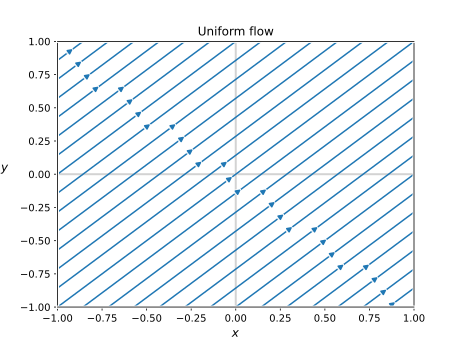
\includegraphics[width=\linewidth]{external/uniformflow.pdf}
\end{image}%
\tcblower
\end{figureptx}%
\end{example}
\begin{example}{Example}{Stagnation point flow.}{example-potential-stagnation}%
\index{stagnation point flow}%
We can verify that the velocity potential%
\begin{equation*}
\phi = \frac{1}{2} (x^2 - y^2),
\end{equation*}
satisfies Laplace's equation. The corresponding velocity field is given by%
\begin{equation*}
[u, v] = [x, -y]. 
\end{equation*}
and corresponds to \emph{stagnation point flow}.%
\par
The streamlines (or velocity field) is shown below.%
\begin{figureptx}{Figure}{Streamlines (or velocity field) of stagnation point flow.}{fig-potential-stagnation}{}%
\begin{image}{0.05}{0.9}{0.05}{}%
\includegraphics[width=\linewidth]{external/stagnationflow.pdf}
\end{image}%
\tcblower
\end{figureptx}%
\end{example}
\begin{example}{Example}{Line source.}{example-potential-linesource}%
\index{line source}%
We aim to derive the potential and velocity for a \emph{line source}, imagined as the flow consisting of a point source or point sink that ejects\slash{}drains fluid from a point in space. Since it would be expected for the potential to be axisymmetric, we attempt to solve \(\nabla^2 \phi = 0\) in plane polar coordinates. This is given by%
\begin{equation*}
\nabla^2 \phi = \frac{1}{r} \pd{}{r}\left(r \pd{\phi}{r}\right) + \frac{1}{r^2} \pd{^2 \phi}{\theta^2} = 0.
\end{equation*}
We assume that the potential takes the form \(\phi = \phi(r)\). Then direct integration gives%
\begin{equation*}
\phi = \frac{Q}{2\pi} \log r, 
\end{equation*}
where we have set an additional constant of integration to zero without loss of generality. The leading constant has been set to \(Q/(2\pi)\) so that \(Q\) can be later identified with a physical quantity.%
\par
The velocity then follows from consideration of the gradient in polar form,%
\begin{equation*}
\bu = \nabla \phi = \pd{\phi}{r} \be_r + \frac{1}{r}\pd{\phi}{\theta} \be_{\theta} = \frac{Q}{2\pi r} \be_r,
\end{equation*}
where the unit vectors written in the Cartesian basis are \(\be_r = [\cos\theta, \sin\theta]\) and \(\be_{\theta} = [-\sin\theta, \cos\theta]\). Thus we can write the velocity as%
\begin{equation*}
\bu = \frac{Q}{2\pi r^2} r[\cos\theta, \sin\theta] = \frac{Q}{2\pi r^2} [x, y].
\end{equation*}
The above corresponds to a velocity field directed radially outwards from the origin. The flow is a called a \emph{line source} because fluid is ejected from the origin (a source). It refers to a "line" because in \((x, y, z)\), the source runs parallel to the \(z\)-axis.%
\par
The streamlines (or velocity field) are shown below.%
\begin{figureptx}{Figure}{Streamlines (or velocity field) of line source flow.}{fig-potential-linesource}{}%
\begin{image}{0.05}{0.9}{0.05}{}%
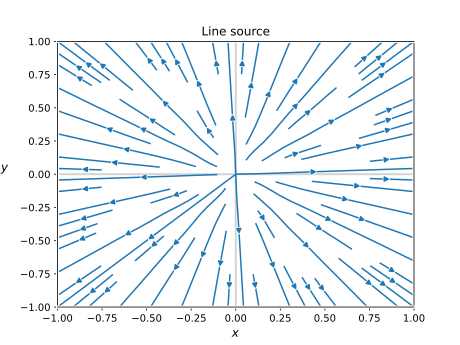
\includegraphics[width=\linewidth]{external/linesource.pdf}
\end{image}%
\tcblower
\end{figureptx}%
Let us also identify the \emph{strength} of this line source. Consider a closed contour \(C\) around the origin. Then the quantity%
\begin{equation*}
\int_C \bu \cdot \bn \, \de{s},
\end{equation*}
is the flux (the flow per unit time) of fluid crossing the contour, with \(\bn\) denoting the unit normal along \(C\).%
\par
For simplicity, let us take the contour \(C\) to be a circle of constant radius \(r = a\). Then since the unit normal is precisely \(\be_r\), we have that%
\begin{equation*}
\int_C \bu \cdot \bn \, \de{s} = \int_0^{2\pi} \frac{Q}{2\pi a} \be_r \cdot \be_r \, (a \, \de\theta) = Q. 
\end{equation*}
In computing the above integral, remember that the conversion following the polar Jacobian is \(\de{s} = r \de{\theta}\) where \(r = a\).%
\par
Therefore, \(Q\) is the rate at which fluid is produced from the line source. If \(Q \lt 0\), we refer to the flow as a \emph{line sink}. \index{line sink}%
\end{example}
Crucially, because the governing fluid mechanical equation is only Laplace's equation: this is a linear partial differential equation, and therefore the summation of elementary flows also produces an admissible flow.%
\begin{example}{Example}{Line source in a uniform flow.}{example-potential-movingsource}%
For instance, we may combine a uniform flow in the \(x\)-direction with a line source:%
\begin{equation*}
\phi = Ux + \frac{Q}{2\pi} \log r = Ux + \frac{Q}{2\pi} \log \sqrt{x^2 + y^2}.
\end{equation*}
We can then obtain the velocity field as%
\begin{equation*}
\bu = [U, 0] + \frac{Q}{2\pi(x^2 + y^2)} [x, y].
\end{equation*}
%
\par
The streamlines (or velocity field) is shown below.%
\begin{figureptx}{Figure}{Streamlines (or velocity field) of a line source in a uniform flow with \(U = 1\) and \(Q = 1\).}{fig-potential-movinglinesource}{}%
\begin{image}{0.05}{0.9}{0.05}{}%
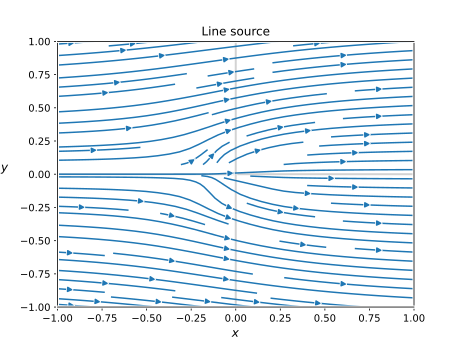
\includegraphics[width=\linewidth]{external/movinglinesource.pdf}
\end{image}%
\tcblower
\end{figureptx}%
Where do you think the stagnation point lies in this flow?%
\end{example}
\end{subsectionptx}
\end{sectionptx}
%
%
\typeout{************************************************}
\typeout{Section 4.2 The streamfunction}
\typeout{************************************************}
%
\begin{sectionptx}{Section}{The streamfunction}{}{The streamfunction}{}{}{sec-streamfunction}
\begin{introduction}{}%
Our next task is to introduce the concept of the \emph{streamfunction}. Remember that in 2D, the irrotational flow led to the equation \hyperref[eqn-2d-irrotational]{({\xreffont\ref{eqn-2d-irrotational}})} and this led to the existence of the potential function. If we begin with incompressibility, however, we have \hyperref[eqn-2d-divu]{({\xreffont\ref{eqn-2d-divu}})}, which can be written as%
\begin{equation}
\nabla \times [-v, u] = 0.\label{eqn-1d-divu-cross}
\end{equation}
And we can deduce the existence of an analogous function, the \emph{streamfunction}, \(\psi(x, y, t)\) satisfying,%
\begin{equation}
u = \pd{\psi}{y} \quad \textrm{and} \quad v = -\pd{\psi}{x}.\label{eqn-2d-uv-streamfunction}
\end{equation}
Alternatively and more conveniently, we can write%
\begin{equation}
\bu = \nabla \times (\psi \bk).\label{eqn-2d-streamfunction}
\end{equation}
To establish the existence of the streamfunction, we follow a similar proof as in \hyperref[thm-exist-potential]{Theorem~{\xreffont\ref{thm-exist-potential}}} but now with the definition that%
\begin{equation}
\psi(x, y, t) = \psi_0(t) + \int_0^{\bx} (u \de{y} - v \de{x}),\label{eqn-streamfunction-def-psi}
\end{equation}
where again \(\psi_0(t)\) is an arbitrary function of \(t\). The proof is otherwise identical, relying on establishing the independence of path of the integral using Stokes' theorem.%
\par
Why all this work? The streamfunction has an intuitive intepretation via the following result.%
\begin{theorem}{Theorem}{The streamfunction is constant along streamlines.}{}{thm-streamfunction}%
The streamfunction, \(\psi(x, y, t)\), is constant along streamlines of the flow (i.e. the trajectory formed by a particle in the flow).%
\end{theorem}
\begin{proof}{Proof}{}{thm-streamfunction-3}
The proof follows simply by the fact that%
\begin{equation*}
\bu \cdot \nabla \psi = \left(\pd{\psi}{y}, -\pd{\psi}{x}\right) \cdot \left(\pd{\psi}{x}, \pd{\psi}{y}\right) = 0,
\end{equation*}
and for which the substitution in the first equality follows from \hyperref[eqn-2d-uv-streamfunction]{({\xreffont\ref{eqn-2d-uv-streamfunction}})}.%
\par
The above equality indicates that the velocity vector, \(\bu\), is orthogonal to the vector pointing along \(\nabla \psi\). However, it is known from Vector Calculus that \(\nabla \psi\) runs along curves of steepest descent\slash{}ascent of \(\psi\)-{}-{}-these must hence be orthogonal to the level sets of \(\psi\). Therefore, the level sets of \(\psi\) are tangential to \(\bu\) (the definition of a streamline).%
\end{proof}
A graphical depiction of the property in \hyperref[thm-streamfunction]{Theorem~{\xreffont\ref{thm-streamfunction}}} is shown below.%
\begin{figureptx}{Figure}{Flow between two streamlines, where the streamlines \(\psi_1\) and \(\psi_2\) are constant. Later, we will consider the flux through the contour \(C\) illustrated in the figure along with its unit normal \(\bn\).}{fig-streamfunction}{}%
\begin{image}{0.15}{0.7}{0.15}{}%
\includegraphics[width=\linewidth]{external/streamfunction.jpg}
\end{image}%
\tcblower
\end{figureptx}%
The streamfunction is thus constant on streamlines. Consider two streamlines. The following theorem relates the flux between the streamlines to the streamline values.%
\begin{theorem}{Theorem}{Flux between streamlines.}{}{thm-flux-streamlines}%
Consider two streamlines \(\psi = \psi_1\) and \(\psi = \psi_2\). We assume that the streamlines pass through the points A and B respectively. Consider a contour \(C\) connecting A and B. The \emph{flux} (net flow of fluid) through \(C\) and hence between the streamlines is%
\begin{equation*}
|\textrm{flux}| = |\psi_2 - \psi_1|
\end{equation*}
We have not specified the sign of the flux as it is subject to the considered direction through \(C\).%
\end{theorem}
\begin{proof}{Proof}{}{thm-flux-streamlines-3}
By definition, the flux is given by the integral%
\begin{equation*}
\int_C \bu \cdot \bn \, \de{s},
\end{equation*}
where \(C\) is any smooth path joining the two streamlines with unit normal \(\bn\), as shown in \hyperref[fig-streamfunction]{Figure~{\xreffont\ref{fig-streamfunction}}}.%
\par
Note that given the curve, and in consideration of a small arclength element \(\de{s}\), the tangent and normal are given by%
\begin{equation*}
\bt = \frac{[\de{x}, \de{y}]}{\sqrt{\de{x}^2 + \de{y}^2}} = \frac{[\de{x}, \de{y}]}{\de{s}}, \qquad 
\bn = \frac{[-\de{y}, \de{x}]}{\de{s}}.
\end{equation*}
Therefore we can write \(\bn \de{s} = [\de{y}, -\de{x}]\). Then the flux is re-written as the following:%
\begin{align*}
\textrm{flux} \amp= \int_C \left[\pd{\psi}{y}, -\pd{\psi}{x}\right] \cdot [\de{y}, \de{x}], \\
\amp= \int_C \left(\pd{\psi}{x} \, \de{x} + \pd{\psi}{y} \right), \\
\amp= \bigl[ \psi \bigr]_C, \\
\amp= \psi(B) - \psi(A), \\
\amp= \psi_2 - \psi_1, 
\end{align*}
In the third line above, \([\psi]_C\) is the change of \(\psi\) across the contour. Note that there is somewhat an arbitrary choice of direction for the contour \(C\), as related to the selection of the normal direction \(\bn\), and the positivity or negativity of the flux. To be safe, we have taken the absolute value in the problem.%
\end{proof}
An example of the use of the above theorem is given in \hyperlink{ps-potential-fluxcalc}{Exercise~{\xreffont 4.7.2}}.%
\begin{example}{Example}{}{sec-streamfunction-2-9}%
Let the velocity of a two-dimensional flow be given by the formula%
\begin{equation*}
\bu = [3ax^2 - 3ay^2, \, -6axy]
\end{equation*}
where \(a\) is a positive constant. By finding the streamfunction, \(\psi\), calculate the volume flux across a curve connecting points \(A = (0, 0)\) and \(B = (1, 1)\) using \hyperref[thm-flux-streamlines]{Theorem~{\xreffont\ref{thm-flux-streamlines}}}.%
\par\smallskip%
\noindent\textbf{\blocktitlefont Solution}.\hypertarget{sec-streamfunction-2-9-2}{}\quad{}(Done in problem class) We can check, using the integration of velocity components that%
\begin{equation*}
\psi = 3ax^2 y - a y^3 + C.
\end{equation*}
Hence the flux is%
\begin{equation*}
Q = \psi(B) - \psi(A) = 2a.
\end{equation*}
We can verify this flux should be positive if the normal is oriented to the right of the curve from A to B.%
\end{example}
Finally, note that the velocity potential was governed by Laplace's equation, \(\nabla^2 \phi = 0\). The streamfunction is also governed by the same Laplace's equation.%
\begin{theorem}{Theorem}{Streamfunction satisfies Laplace's equation.}{}{thm-streamfunction-laplace}%
Like the velocity potential, the streamfunction satisfies Laplace's equation:%
\begin{equation}
\pd{^2 \psi}{x^2} + \pd{^2 \psi}{y^2} = \nabla^2 \psi = 0.\label{eqn-2d-streamfunction-laplace}
\end{equation}
%
\end{theorem}
\begin{proof}{Proof}{}{thm-streamfunction-laplace-3}
Substitute the relationship \hyperref[eqn-2d-uv-streamfunction]{({\xreffont\ref{eqn-2d-uv-streamfunction}})} into \hyperref[eqn-2d-irrotational]{({\xreffont\ref{eqn-2d-irrotational}})}.%
\end{proof}
Like in the situation of certain flows, e.g. the line source in \hyperref[example-potential-linesource]{Example~{\xreffont\ref{example-potential-linesource}}}, it is easier to work in alternative coordinate systems to study the streamfunction. Since we know that \(\bu = \nabla \times (\psi \bk)\) by \hyperref[eqn-2d-streamfunction]{({\xreffont\ref{eqn-2d-streamfunction}})}, we can use the conversion of the curl to polar coordinates in \hyperref[eqn-identity-curlpolar]{({\xreffont\ref{eqn-identity-curlpolar}})} to give%
\begin{equation}
u_r = \frac{1}{r} \pd{\psi}{\theta} \quad \textrm{and} \quad u_{\theta} = -\pd{\psi}{r}\,\label{eqn-streamfunction-polar}
\end{equation}
which allows us to relate the radial and angular velocities to the streamfunction.%
\end{introduction}%
%
%
\typeout{************************************************}
\typeout{Subsection 4.2.1 Elementary flows}
\typeout{************************************************}
%
\begin{subsectionptx}{Subsection}{Elementary flows}{}{Elementary flows}{}{}{sec-streamfunction-3}
Let us return to each of the examples in \hyperref[sec-Potential-and-streamfunction]{Section~{\xreffont\ref{sec-Potential-and-streamfunction}}} and reconsider their corresponding streamfunctions.%
\begin{example}{Example}{Uniform flow.}{sec-streamfunction-3-3}%
\index{uniform flow, streamfunction}%
From \hyperref[example-potential-uniform]{Example~{\xreffont\ref{example-potential-uniform}}}, we can directly integrate \(u = \psi_y\) and \(v = -\psi_x\) to get%
\begin{equation*}
\psi = Uy\cos\alpha - Ux\sin\alpha, 
\end{equation*}
up to an arbitrary constant. Therefore, lines of constant \(\psi\) correspond to%
\begin{equation*}
y = x\tan\alpha + \textrm{constant},
\end{equation*}
which indeed yields the image seen in \hyperref[fig-potential-uniform]{Figure~{\xreffont\ref{fig-potential-uniform}}}.%
\end{example}
\begin{example}{Example}{Stagnation point flow.}{sec-streamfunction-3-4}%
\index{stagnation point flow, streamfunction}%
Now turning to \hyperref[example-potential-stagnation]{Example~{\xreffont\ref{example-potential-stagnation}}}, we integrate \(u = y = \psi_x\) and \(v = x = \psi_y\). This gives%
\begin{equation*}
\psi = xy, 
\end{equation*}
up to an arbitrary constant. Indeed curves of constant \(\psi\) match the hyperbole shown in \hyperref[fig-potential-stagnation]{Figure~{\xreffont\ref{fig-potential-stagnation}}}.%
\end{example}
\begin{example}{Example}{Line source.}{example-streamfunction-linesource}%
\index{line source, streamfunction}%
For the situation of the line source in \hyperref[example-potential-linesource]{Example~{\xreffont\ref{example-potential-linesource}}}, we want to work with polar coordinates. From the previous work, we have for this situation the potential \(\phi = Q/(2\pi log r\). It then follows from the polar version of the gradient in \hyperref[eqn-identity-grad-polar]{({\xreffont\ref{eqn-identity-grad-polar}})}, that the velocity is entirely radial and%
\begin{equation}
\bu = \pd{\phi}{r}\be_r + 0 = \frac{Q}{2\pi r} \be_r.\label{eqn-streamfunction-u-linesource}
\end{equation}
We use the formulae in \hyperref[eqn-streamfunction-polar]{({\xreffont\ref{eqn-streamfunction-polar}})} and integrate \(\frac{1}{r} \pd{\psi}{\theta} = \frac{Q}{2\pi r}\) yielding%
\begin{equation*}
\psi = \frac{Q}{2\pi} \theta.
\end{equation*}
Then indeed note that the lines of constant \(\psi\) are given by the radial lines of constant \(\theta\), matching the illustration in \hyperref[fig-potential-linesource]{Figure~{\xreffont\ref{fig-potential-linesource}}}.%
\end{example}
Another remark concerns the fact that \(\psi\) is a multi-valued function in the example of the line source \hyperref[example-streamfunction-linesource]{Example~{\xreffont\ref{example-streamfunction-linesource}}}, gaining a jump of \(Q\) every time the origin is encircled. This is indeed a warning that the standard proof, analogous to \hyperref[thm-exist-potential]{Theorem~{\xreffont\ref{thm-exist-potential}}}, leading to the existence of a unique streamfunction, via \hyperref[eqn-streamfunction-def-psi]{({\xreffont\ref{eqn-streamfunction-def-psi}})} would not apply since the velocity field \hyperref[example-streamfunction-linesource]{Example~{\xreffont\ref{example-streamfunction-linesource}}} is not defined at the origin. However, despite this, we see that the streamfunction provides well-defined predictions of streamlines on the \emph{cut} plane with e.g. \(\theta \in [0, 2\pi)\).%
\begin{example}{Example}{Line source in a uniform flow.}{sec-streamfunction-3-7}%
Like the case of the potential function in \hyperref[example-potential-movingsource]{Example~{\xreffont\ref{example-potential-movingsource}}}, the linearity of the equation governing the streamfunction implies that we can consider the combination of those streamfunctions for a line source with a uniform flow. This yields%
\begin{equation*}
\psi = Uy + \frac{Q}{2\pi}\theta, 
\end{equation*}
for the case of uniform flow of speed \(U\) in the positive \(x\)-direction. The streamlines are then given by%
\begin{equation*}
Uy + \frac{Q}{2\pi} \theta = \frac{Q}{2\pi}C,
\end{equation*}
having designed the constant combination on the right hand-side for convenience. Then using \(y = r\sin\theta\), we have%
\begin{equation*}
r = \left(\frac{Q}{2\pi U}\right) \frac{C - \theta}{\sin\theta}.
\end{equation*}
%
\end{example}
Our previous examples were reliant on considering the flows generated by the velocity potentials studied previously. However, we can also consider "fundamental solutions" of the equation \(\nabla^2 \psi = 0\) in their own right. Recall that in deriving the velocity potential of the line source in \hyperref[example-potential-linesource]{Example~{\xreffont\ref{example-potential-linesource}}}, we considered the solution of an axi-symmetric problem, where \(\phi = \phi(r)\) is only dependent on the distance from the origin. A similar argument must imply that the analogous axi-symmetric streamfunction is a permissible solution. And this leads us to the following example.%
\begin{example}{Example}{Line vortex.}{example-streamfunction-linevortex}%
\index{line vortex}%
The fundamental solution for the streamfunction, in plane polar coordinates, is the axisymmetric solution,%
\begin{equation}
\psi = -\frac{\Gamma}{2\pi}\log r,\label{eqn-streamfunction-linevortex}
\end{equation}
defined up to a constant, and corresponds to a \emph{line vortex}.%
\par
The streamlines of such a flow correspond to circular trajectories with \(r\) constant, and are visualised in %
\begin{figureptx}{Figure}{Streamlines (or velocity field) of a line vortex with \(\Gamma = 1\).}{fig-streamfunction-linevortex}{}%
\begin{image}{0.05}{0.9}{0.05}{}%
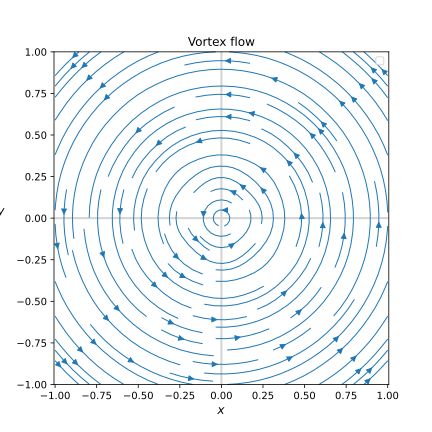
\includegraphics[width=\linewidth]{external/linevortex.pdf}
\end{image}%
\tcblower
\end{figureptx}%
Recall that the radial and angular velocities are given by \hyperref[eqn-streamfunction-polar]{({\xreffont\ref{eqn-streamfunction-polar}})}. Therefore, we see that the velocity vector is given by%
\begin{equation}
\bu = -\pd{\psi}{r} \be_{\theta} = \frac{\Gamma}{2\pi r} \be_{\theta},\label{eq-u-line-vortex}
\end{equation}
and thus this flow corresponds to entirely circular trajectories orbiting the origin, and with angular velocity increasing as \(r \to 0\).%
\par
The quantity \(\Gamma\) is called the \emph{vortex strength}, analogous to the source strength \(Q\) in \hyperref[example-potential-linesource]{Example~{\xreffont\ref{example-potential-linesource}}}. Let us consider the amount of circulation around a contour \(C\) that contains the origin:%
\begin{equation*}
\oint_C \bu \cdot \de{\bx} = \oint_C (u \, \de{x} + v \, \de{y}),
\end{equation*}
i.e. one envisions encircling the origin along \(C\), adding up each of the velocity components tangential to the path. This is the circulation. By Stokes' theorem it is equal to the flux of vorticity of the corresponding bounding surface.%
\par
Choosing \(C\) to be the circle of radius \(r = a\), we have \(\de{\bx} = a \be_{\theta} \de{\theta}\). Then the circulation is given by%
\begin{equation}
\oint_C \bu \cdot \de{\bx} = \int_0^{2\pi} \frac{\Gamma}{2\pi a} \be_{\theta} \cdot \be_{\theta} a \de\theta = \Gamma.\label{eq-line-vortex-circulation}
\end{equation}
So indeed this gives us an intuitive understanding of \(\Gamma\). Notice that \(\Gamma \gt 0\) corresponds to flow in the anticlockwise sense, and \(\Gamma \lt 0\) corresponds to flow in the clockwise sense.%
\par
In \hyperlink{ps-streamfunction-flux-compute}{Exercise~{\xreffont 4.7.1}}, you will practice the computation of fluxes using line integrals.%
\end{example}
\end{subsectionptx}
\end{sectionptx}
%
%
\typeout{************************************************}
\typeout{Section 4.3 The complex potential}
\typeout{************************************************}
%
\begin{sectionptx}{Section}{The complex potential}{}{The complex potential}{}{}{sec-complex-potential}
\begin{introduction}{}%
In the previous two sections, we studied the properties and utility of the velocity potential \(\phi\) and streamfunction \(\psi\) in the context of two-dimensional potential flows (inviscid, incompressible, irrotational). We did this with techniques from real-valued Vector Calculus.  As it turns out, there is a much more elegant and powerful framework for studying two-dimensional flow which leverages the significant power of complex analysis and complex variables.%
\par
In fact, you may have already noticed this on an intuitive level, given the intimate relationships between \(\phi\) and \(\psi\), seeming to exhibit a certain kind of symmetry in formulae and operations. Complex analysis is the language in which we can make this kind of "symmetry" transparent.%
\par
We begin by reviewing (or in some cases, introducing) you to some key theorems about the properties of well-behaved (analytic) complex functions.%
\par
In his section, we will refer to a complex function generically as%
\begin{equation*}
f(z) = u(x, y) + \im v(x, y)
\end{equation*}
where \(u\) and \(v\) and the real-valued decompositions of the complex-valued function \(f\). Also, \(z = x + \im y\).%
\par
A complex function is differentiated in much the same way as real-valued functions, with the definition that%
\begin{equation}
f'(z) = \lim_{\Delta z \to 0} \frac{f(z + \Delta z) - f(z)}{\Delta z}.\label{eqn-complex-derivative}
\end{equation}
The crucial difference with real-valued differentiation is that the above limit is required to hold whilst approaching the point \(z\) in any direction of the complex plane.%
\begin{remark}{Remark}{}{sec-complex-potential-2-6}%
As long as you stay away from exceptional points of a function, the "calculus" of complex functions is largely the same as for real-valued functions, e.g.%
\begin{gather*}
\dd{(z^m)}{z} = mz^{m-1}, \qquad \dd{\e^z}{z} = \e^z,\\
\dd{(\log (z+1))}{z} = \frac{1}{z + 1}, \quad \dd{\sin(z^2)}{z} = 2z\cos(z^2). 
\end{gather*}
and the usual rules of algebraic manipulations hold. There are some caveats, however, which are dealt with on an individual manner.%
\end{remark}
\begin{remark}{Remark}{Examinable content.}{sec-complex-potential-2-7}%
The proofs of all theorems from this section are non-examinable, but you are expected to understand the theorems and their relevance to the theory of potential flow.%
\end{remark}
Below, we will often use susbcripts for partial differentiation, e.g. \(u_x = \pd{u}{x}\).%
\end{introduction}%
%
%
\typeout{************************************************}
\typeout{Subsection 4.3.1 Cauchy's theorem and harmonic functions}
\typeout{************************************************}
%
\begin{subsectionptx}{Subsection}{Cauchy's theorem and harmonic functions}{}{Cauchy's theorem and harmonic functions}{}{}{subsec-complex-introduction}
We will follow the reference text by \hyperlink{ref-kreyszig}{[{\xreffont 2}]} and \hyperlink{ref-fornberg}{[{\xreffont 6}]}  and introduce the basic notions of complex functions that we will need.%
\begin{definition}{Definition}{Analyticity.}{def-analytic}%
\index{analytic}%
A function \(f: \mathbb{C} \to \mathbb{C}\) is said to be analytic in a domain if \(f(z)\) is defined and differentiable at all points in the domain. The function is said to be \emph{analytic at a point} \(z = z_0\) if it is analytic in a neighbourhood of \(z_0\).%
\par
When we refer to an \emph{analytic function}, we mean a function that is analytic in some domain of \(\mathbb{C}\) (often clear by context).%
\par
The function is \emph{holomorphic}\index{holomorphic} if it is analytic; the terms are synonyms.%
\par
An analytic function is \emph{entire}\index{entire} if its region of analyticity includes all points in \(\mathbb{C}\), including infinity.%
\end{definition}
Note that above, we have stated that a function is analytic if it is well-defined and differentiable \emph{once}(!) As it turns out, the requirement that a complex-valued function is differentiable is a strong condition. An analytic function turns out to be infinitely differentiable by consequence!%
\begin{remark}{Remark}{}{subsec-complex-introduction-5}%
In this module, we will not be concerned with formalities when they are not relevant. For example, in our definition of analyticity, we do not specify if the relevant domains are open or closed. The functions we work with are generally non-pathological-{}-{}-they may have isolated singularities or exceptional points, but generally the application and context will make it clear the limits of our results.%
\end{remark}
Now we have one of the most important theorems of complex analysis.%
\begin{theorem}{Theorem}{Cauchy-Riemann equations I.}{}{thm-CR1}%
If \(f(z) = u(x, y) + \im v(x, u)\) is differentiable, then the Cauchy-Riemann equations, given by%
\begin{equation}
u_x = v_y \quad \text{and} \quad u_y = -v_x,\label{eqn-CR}
\end{equation}
hold.%
\par
In particular, if \(f\) is analytic on a domain, then its real and complex parts must satisfy the Cauchy-Riemann equations \hyperref[eqn-CR]{({\xreffont\ref{eqn-CR}})} (in that domain).%
\end{theorem}
\begin{proof}{Proof}{}{thm-CR1-3}
(Non-examinable)%
\par
This follows by considering the definition of the derivative \hyperref[eqn-complex-derivative]{({\xreffont\ref{eqn-complex-derivative}})} when the point \(z\) is approached from the \(x\) or \(y\) directions.%
\par
With \(\Delta z = \Delta x\) real, we can verify from applying the definition that%
\begin{equation*}
f'(z) = \pd{u}{x} + \im \pd{v}{x}.
\end{equation*}
On the other hand, approaching with \(\Delta z = \im \Delta y\) gives%
\begin{equation*}
f'(z) = -\im \pd{u}{y} + \pd{v}{y}. 
\end{equation*}
Equating the two results then yields the Cauchy-Riemann equations.%
\end{proof}
It turns out that the Cauchy-Riemann equations are not only necessary to an analytic function, but are actually sufficient as well.%
\begin{theorem}{Theorem}{Cauchy-Riemann equations II.}{}{thm-CR2}%
If two real-valued continuous functions, \(u(x, y)\) and \(v(x, y)\) of two real variables \(x\) and \(y\) have continuous firsst partial derivatives that satisfy the Cauchy-Riemann equations \hyperref[eqn-CR]{({\xreffont\ref{eqn-CR}})} in some domain, then \(f(z) = u(x, y) + \im v(x, y)\) is analytic in that domain.%
\end{theorem}
\begin{proof}{Proof}{}{thm-CR2-3}
(Non-examinable)%
\par
The proof is not difficult, but we will refer students to \hyperlink{ref-kreyszig}{[{\xreffont 2}]} for its proof. It relies on constructing the derivative of \(f\) along any direction using the decomposition into the two Cartesian directions.%
\end{proof}
\begin{theorem}{Theorem}{}{}{thm-complex-inf-derivatives}%
If \(f\) is analytic, it is differentiable to all orders.%
\end{theorem}
Our last step involves relating complex functions to the solution of Laplace's equation(s), i.e. \hyperref[eqn-2d-laplace]{({\xreffont\ref{eqn-2d-laplace}})} or \hyperref[eqn-2d-streamfunction-laplace]{({\xreffont\ref{eqn-2d-streamfunction-laplace}})}, that govern potential flow.%
\begin{theorem}{Theorem}{Analyticity and Laplace's equation.}{}{thm-complex-laplace}%
If \(f(z) = u(x, y) + \im v(x, y)\) is analytic in a domain \(D\), then \(u\) and \(v\) satisfy Laplace's equation,%
\begin{equation*}
\nabla^2 u = u_{xx} + u_{yy} = 0 \quad \textrm{and} \quad
\nabla^2 v = v_{xx} + v_{yy} = 0,
\end{equation*}
in \(D\), and have continuous second partial derivatives in \(D\).%
\end{theorem}
\begin{proof}{Proof}{}{thm-complex-laplace-3}
Since \(f\) is analytic, then it follows from \hyperref[thm-CR1]{Theorem~{\xreffont\ref{thm-CR1}}} that \(u_x = v_y\) and \(u_y = -v_x\). It furthermore follows from \hyperref[thm-complex-inf-derivatives]{Theorem~{\xreffont\ref{thm-complex-inf-derivatives}}} that \(f\) is differentiable to all orders; therefore, we can take derivatives to obtain%
\begin{equation*}
u_{xx} = v_{yx} \quad \text{and} \quad -u_{yy} = v_{xy}. 
\end{equation*}
The second derivatives are continuous and therefore \(v_{xy} = v_{yx}\). Therefore \(u_{xx} + u_{yy} = 0\). Laplace's equation is analogously proved for \(v\).%
\end{proof}
The above theorem is truly a remarkable result; it would not be a stretch to state that this single result was at the forefront of why complex analysis played such an important role in the development of applied mathematics and physics in the 18th, 19th, and 20th centuries.%
\par
Since Laplace's equation, \(\nabla^2 \phi = 0\), is such an important equation in physics, occuring in theories of gravitation, electrostatics, fluid mechanics, etc. the theorem establishes that there exists a parallel theory in the language of complex variables for the specific case of two-dimensional applications.%
\par
A potential fluid, for example, can be studied by manipulating complex functions of the form%
\begin{equation*}
f(z) = \phi(x, y) + \im \psi(x, y).
\end{equation*}
One can envision all kinds of different forms of \(f\)-{}-{}-polynomials, cosines and sines, exponentials, logarithms, etc. As long as the function is locally differentiable, it is thus analytic and therefore can be associated with (some kind of) fluid flow.%
\end{subsectionptx}
%
%
\typeout{************************************************}
\typeout{Subsection 4.3.2 Examples of elementary flows}
\typeout{************************************************}
%
\begin{subsectionptx}{Subsection}{Examples of elementary flows}{}{Examples of elementary flows}{}{}{subsec-complex-examples}
Let us return to the examples of flows studied in \hyperref[sec-Potential-and-streamfunction]{Section~{\xreffont\ref{sec-Potential-and-streamfunction}}} and re-interpret them using the theory of analytic functions.%
\par
We will associate the velocity potential, \(\phi\), and streamfunction \(\psi\) with an analytic function in the following way.%
\begin{definition}{Definition}{}{def-complex-potential}%
Let \(\phi(x,y)\) and \(\psi(x, y)\) be the respective velocity potential and streamfunction for some potential flow. We define%
\begin{equation}
f(z) = \phi(x, y) + \im \psi(x, y),\label{eqn-complex-potential}
\end{equation}
and call \(f\) the \emph{complex potential}.%
\par
Note that by differentiating in the horizontal and vertical directions, we have%
\begin{equation*}
\dd{f}{z} = \pd{}{x} (\phi + \im \psi) = \pd{}{y} (\phi + \im \psi). 
\end{equation*}
Therefore it follows that the horizontal and vertical velocity components of the flow, related via \(\bu = [u, v]\), are given by%
\begin{equation}
\dd{f}{z} = u - \im v.\label{eqn-complex-velocity}
\end{equation}
%
\end{definition}
\begin{example}{Example}{Uniform flow.}{subsec-complex-examples-5}%
\index{uniform flow, complex}%
We can verify that the complex potential for uniform flow is given from%
\begin{equation*}
f(z) = U \e^{-\im \alpha} z.
\end{equation*}
This can be compared to  \hyperref[example-potential-uniform]{Example~{\xreffont\ref{example-potential-uniform}}}.%
\end{example}
\begin{example}{Example}{Stagnation point flow.}{subsec-complex-examples-6}%
\index{stagnation point flow, complex}%
We can verify that the complex potential for a stagnation point flow is given by%
\begin{equation*}
f(z) = \frac{z^2}{2}.
\end{equation*}
This can be compared to  \hyperref[example-potential-stagnation]{Example~{\xreffont\ref{example-potential-stagnation}}}.%
\end{example}
\begin{example}{Example}{Line source.}{subsec-complex-examples-7}%
\index{line source, complex}%
We can verify that the complex potential for a line source flow is given by%
\begin{equation}
f(z) = \frac{Q}{2\pi} \log z\label{eqn-complex-linesource}
\end{equation}
This can be compared to  \hyperref[example-potential-linesource]{Example~{\xreffont\ref{example-potential-linesource}}}.%
\par
The complex logarithm is an example of a function that is not analytic at the isolated point \(z = 0\) where it possesess a \emph{branch point}. However, it still provides a permissible analytic function away from the origin.%
\par
The evaluation of the complex logarithm can be performed via the definition%
\begin{equation}
\log z = \log r + \im \theta,\label{eqn-complex-logarithm}
\end{equation}
where \(z = r\e^{\im \theta}\) is the polar form representation of \(z\). In particular \(log z\) is a multi-function with a \emph{branch point} at the origin.%
\par
With the above decomposition of the logarithm in mind, notice that we can then conclude that the velocity potential and streamfunction are given by%
\begin{equation*}
\phi = \Re[f] = \frac{Q}{2\pi} \log r \quad \text{and} \quad
\psi = \Im[f] = \frac{Q}{2\pi} \theta.
\end{equation*}
Indeed the streamlines are along the rays \(\theta\) constant.%
\par
From \hyperref[eqn-complex-linesource]{({\xreffont\ref{eqn-complex-linesource}})}, we can also compute the velocities using the relationship \hyperref[eqn-complex-velocity]{({\xreffont\ref{eqn-complex-velocity}})}. We thus have%
\begin{equation*}
u - \im v = \frac{Q}{2\pi} \frac{1}{z} = \frac{Q}{2\pi} \frac{x - \im y}{(x^2 + y^2)},
\end{equation*}
once we have multiplied the top and bottom by the conjugate of \(z\).%
\end{example}
\begin{example}{Example}{Line vortex flow.}{example-complexpotential-linevortex}%
\index{line vortex, complex}%
We can verify that the complex potential for a line vortex is given by%
\begin{equation}
f(z) = -\frac{\im \Gamma}{2\pi} \log z.\label{eq-line-vortex-complex-potential}
\end{equation}
This can be compared to  \hyperref[example-streamfunction-linevortex]{Example~{\xreffont\ref{example-streamfunction-linevortex}}}.%
\par
Again, using the definition of the complex logarithm, via \hyperref[eqn-complex-logarithm]{({\xreffont\ref{eqn-complex-logarithm}})}, we can write \(f\) in terms of its real and complex components as%
\begin{equation*}
f(z) = \frac{\Gamma}{2\pi} (\theta - \im \log r),
\end{equation*}
where \(z = r\e^{\im\theta}\).%
\par
Therefore, the streamfunction is given by \(\psi = -(\Gamma/2\pi) \log r\) and is constant along circular trajectories with constant distance from the origin, \(r\).%
\end{example}
\end{subsectionptx}
\end{sectionptx}
%
%
\typeout{************************************************}
\typeout{Section 4.4 The method of images}
\typeout{************************************************}
%
\begin{sectionptx}{Section}{The method of images}{}{The method of images}{}{}{sec-method-of-images}
\begin{introduction}{}%
The preceeding sections would give the misleading impression that solving potential-flow problems for two-dimensional flows is easy. This is not the case, and the primary reason is due to the presence of \emph{boundary conditions}. The elementary flows we have previously considered were unconfined and\slash{}or we did not consider additonal constraints on their behaviours at infinity. In reality, a real physical fluid, whether in the ocean, the air, or in a container, is confined in some direction, and we must often consider subtle questions about the mechanism that produces the fluid motion.%
\par
In this section, we consider the situation of solving for the potential flow in a fluid region with boundaries. Recall that this is equivalent to finding a velocity potential satisfying \(\nabla^2 \phi = 0\) or an analytic complex potential, \(f(z)\).%
\par
Recall from \hyperref[note-noflux-BC]{Note~{\xreffont\ref{note-noflux-BC}}} that on solid boundaries, we must impose the no-flux condition that%
\begin{equation*}
\bu \cdot \bn = \nabla \phi \cdot \bn = 0 \quad \text{on $\partial V$}.
\end{equation*}
%
\end{introduction}%
%
%
\typeout{************************************************}
\typeout{Subsection 4.4.1 Planar boundaries: a half-plane}
\typeout{************************************************}
%
\begin{subsectionptx}{Subsection}{Planar boundaries: a half-plane}{}{Planar boundaries: a half-plane}{}{}{subsec-images-planar}
Consider the situation illustrated in \hyperref[image-planar01]{Figure~{\xreffont\ref{image-planar01}}}.%
\begin{figureptx}{Figure}{A flow region in the right half-plane, with a single source placed at \(x = d\).}{image-planar01}{}%
\begin{image}{0.1}{0.8}{0.1}{}%
\includegraphics[width=\linewidth]{external/image-planar01.jpg}
\end{image}%
\tcblower
\end{figureptx}%
We envision a semi-infinite region of fluid bounded on the left by a wall at \(x = 0\). A single (line) source of strength \(Q\) is placed at \(x = d\). Therefore from \hyperref[eqn-complex-linesource]{({\xreffont\ref{eqn-complex-linesource}})}, we would expect that at least near \(x = d\), the complex potential behaves as%
\begin{equation*}
f(z) \sim \frac{Q}{2\pi} \log (z-d) \quad \text{as $z \to d$}.
\end{equation*}
However the above solution does not satisfy the required boundary conditions at \(x = 0\) since it corresponds to a velocity field for which the horizontal velocity penetrates through \(x = 0\). This can be verified via inspection. For example, we can inspect the velocity or the streamlines; this is part of \hyperlink{ps-image-planar01}{Exercise~{\xreffont 4.7.4}}.%
\par
Rephrased in terms of the streamlines, the boundary condition at \(x = 0\) is equivalent to the constraint that%
\begin{equation*}
\Im f(z) = \psi = \textrm{constant at $x = 0$}.
\end{equation*}
%
\par
Our inspired solution to the above problem is referred to as \emph{the method of images}.%
\begin{note}{Note}{Method of images.}{note-method-of-images}%
Given potential flow problem, we consider the superposition of elementary sinks\slash{}sources, i.e.%
\begin{equation*}
f(z) = \frac{1}{2\pi} \sum_{j=0}^{N-1} Q_j \log(z - z_j), 
\end{equation*}
and\slash{}or vortices,%
\begin{equation*}
f(z) = -\frac{\im}{2\pi} \sum_{j=0}^{N-1} \Gamma_j \log(z - z_j).
\end{equation*}
The strengths and locations of the individual contributions are chosen so that boundary conditions on the required boundaries (including at infinity) can be met.%
\end{note}
Notice that the \emph{linearity} of the potential flow problem is crucial: any analytic function is associated with a velocity potential that satisfies Laplace's equation, \(\nabla^2 \phi = 0\), and therefore the superposition of such functions also yields a permissible complex potential, \(f\).%
\par
We consider the addition of a "fictitious" image source, with the same strength at the reflected point \(x = -d\), which lies outside of the posited fluid region. This gives the complex potential of%
\begin{equation*}
f(z) = \frac{Q}{2\pi} \log(z - d) + \frac{Q}{2\pi} \log(z + d). 
\end{equation*}
This yields the illustration of the flow in \hyperref[fig-image-planar02]{Figure~{\xreffont\ref{fig-image-planar02}}}%
\begin{figureptx}{Figure}{Placement of the image source at \(x = -d\) makes it so the boundary condition on \(x = 0\) can be satisfied.}{fig-image-planar02}{}%
\begin{image}{0.1}{0.8}{0.1}{}%
\includegraphics[width=\linewidth]{external/image-planar02.jpg}
\end{image}%
\tcblower
\end{figureptx}%
The corresponding complex velocity is given by%
\begin{equation*}
u - \im v = f'(z) = \frac{Q}{2\pi}\frac{z}{z^2 - d^2}.
\end{equation*}
So indeed, on the central boundary, we have \(z = \im y\), and%
\begin{equation*}
u - \im v = - \im \frac{Q}{\pi} \frac{y}{y^2 + d^2},
\end{equation*}
and the velocity is entirely vertical. So indeed, the condition that \(\bu \cdot \bn = 0\) on the planar boundary is satisfied.%
\par
In order to study the complex velocity, \(f(z)\), and develop an equation for the streamlines of the flow, we must first navigate the fact that the complex logarithm function is only well-defined in a slit complex plane. First, let%
\begin{equation*}
z - d = r_1 \e^{\im \theta_1} \quad \textrm{and} \quad z + d = r_2 \e^{\im \theta_2}.
\end{equation*}
Using the definition of the complex logarithm \hyperref[eqn-complex-logarithm]{({\xreffont\ref{eqn-complex-logarithm}})}, we have%
\begin{equation*}
f(z) = \frac{Q}{2\pi} \left[ \log r_1 + \log r_2\right] + \im \frac{Q}{2\pi}\left[ \theta_1 + \theta_2 \right].
\end{equation*}
The definitions of \(r_1, r_2\) and \(\theta_1, \theta_2\), are shown in the below figure. In order for each logarithm to be well defined, the angles \(\theta_1\) and \(\theta_2\) must be restricted to be less than a complete revolution. We thus restrict \(\theta_1 \in [0, 2\pi)\) and \(\theta_1 \in [-\pi, \pi)\).%
\begin{figureptx}{Figure}{When considering the evaluation of the flow, we must take care of the fact that the logarithm is multi-valued. A branch cut from each of the two branch points is imposed.}{fig-image-duallog}{}%
\begin{image}{0}{1}{0}{}%
\includegraphics[width=\linewidth]{external/image-duallog.jpg}
\end{image}%
\tcblower
\end{figureptx}%
In \hyperlink{ps-image-planar02}{Exercise~{\xreffont 4.7.5}}, you will be asked to develop an equation for the streamlines of this flow.%
\par
The above ideas can be extended to the situation of a line vortex in a half plane. Again, we are interested in describing the flow due to a line vortex at \(z = d\), and therefore we expect that near this point,%
\begin{equation*}
f(z) \sim -\frac{\im\Gamma}{2\pi} \log(z - d) \quad \textrm{as $z \to d$}.
\end{equation*}
However, the above potential does not satisfy the necessary zero-flux condition at \(x = 0\).%
\par
In this case, the approach is to add an image vortex at \(z = -d\), but opposite in direction:%
\begin{equation*}
f(z) = -\frac{\im\Gamma}{2\pi} \log(z - d) + \frac{\im\Gamma}{2\pi} \log(z + d).
\end{equation*}
Therefore, this flow is composed by a line vortex circulating anticlockwise on the right, and a line vortex circulating clockwise on the left. It can be verified that the complex velocity is given by%
\begin{equation*}
u - \im v = -\frac{\im \Gamma d}{\pi(z^2 - d^2)}
\end{equation*}
and indeed the velocity at \(x = 0\) is entirely vertical and there is no flux through the boundary.%
\par
There is an exercise in \hyperlink{ps-image-planar03}{Exercise~{\xreffont 4.7.6}}.%
\begin{remark}{Remark}{Uniqueness of solutions.}{subsec-images-planar-18}%
You may be wondering: if a permissible potential function is found that satisfies the necessary boundary conditions, can we be certain it is the unique solution in the problem (up to a constant)? You may understand the construction of potentials, via the method of images, but perhaps irked that it involves the insertion of these so-called 'fictitious' points. The answer, at least for most non-pathological problems in potential flow theory (i.e. all the problems you study) is \emph{yes}, the solution you have found is assured to be the only solution (up to a constant).%
\par
This is, to some extent, related to the \href{https://proofwiki.org/wiki/Uniqueness_of_Analytic_Continuation}{uniqueness of analytic continuation}. In a nutshall, the relevant theorem states that given two admissible complex potentials, say \(f_1(z)\) and \(f_2(z)\), that agree on the line \(x = 0\) (in the case of the above situation), it is the case that \(f_1 = f_2\) everywhere (where they are analytic).%
\par
Therefore, you can be certain that solutions you find via the trick of method of images are the only solutions.%
\end{remark}
\end{subsectionptx}
\end{sectionptx}
%
%
\typeout{************************************************}
\typeout{Section 4.5 Conformal mapping}
\typeout{************************************************}
%
\begin{sectionptx}{Section}{Conformal mapping}{}{Conformal mapping}{}{}{sec-conformal-mapping}
\begin{introduction}{}%
The essential idea of conformal mapping is as follows. Suppose that we are given a two-dimensional potential fluid flow problem in a region, \(R \subseteq \mathbb{C}\), with impermeable boundary \(\partial R\). There may be singularities in \(R\) corresponding to sinks, sources, vortices, etc. We then seek a \emph{conformal mapping} from the \(z\)-plane to the \(\zeta\)-plane via%
\begin{equation*}
\zeta = g(z),
\end{equation*}
so that the region \(R\) is mapped to a new region \(\hat{R} \subseteq \mathbb{C}\), as shown in \hyperref[fig-conformal-general]{Figure~{\xreffont\ref{fig-conformal-general}}}.%
\par
The hope is that within the \(\zeta\)-plane, the fluid region is sufficiently simple that a complex potential, say \(F(\zeta)\), can be found. This task is aided by virtue of the fact that sinks\slash{}sources and vortices are preserved by the conformal map. Typically, we wish for \(\hat{R}\) to be e.g. the upper half-plane or the unit disc, with \(\partial\hat{R}\) to be the real axis or circumferance of the unit disc, respectively. Once found, the complex potential in the \(z\)-plane is then obtained simply by inverting the conformal map, i.e.%
\begin{equation*}
f(z) = F(g(\zeta)) = \phi(x, y) + \im \psi(x, y).
\end{equation*}
This simple idea turns out to yield many insights to potential flows in two dimensions.%
\begin{figureptx}{Figure}{A general conformal mapping from the \(z\)-plane to the \(\zeta\)-plane. The object is to map the region \(R\) to the region \(\hat{R}\), which is geometrically simpler.}{fig-conformal-general}{}%
\begin{image}{0}{1}{0}{}%
\includegraphics[width=\linewidth]{external/conformal_generalmap.jpg}
\end{image}%
\tcblower
\end{figureptx}%
\end{introduction}%
%
%
\typeout{************************************************}
\typeout{Subsection 4.5.1 Source in a wedge}
\typeout{************************************************}
%
\begin{subsectionptx}{Subsection}{Source in a wedge}{}{Source in a wedge}{}{}{sec-conformal-mapping-3}
Consider fluid contained in a wedge with walls at \(\theta = 0\) and \(\theta = \alpha > 0\), and with the fluid in \(0 < \theta < \alpha\). A source of strength \(Q\) is placed somewhere within the flow, say at the point \(z = c\).%
\par
Consider then the map%
\begin{equation}
\zeta = g(z) = z^{\pi/\alpha}.\label{eqn-conformal-wedge-map}
\end{equation}
It can be verified that this map transforms the fluid region to the upper half-\(\zeta\)-plane. Indeed the ray \(\theta = 0\) is mapped to the positive real axis and the ray \(\theta = \alpha\) is mapped to the negative real axis. This is shown in \hyperref[fig-conformal-wedge]{Figure~{\xreffont\ref{fig-conformal-wedge}}}.%
\begin{figureptx}{Figure}{The map from the wedge-shaped region in the \(z\)-plane (left) and the upper half-\(\zeta\)-plane (right).}{fig-conformal-wedge}{}%
\begin{image}{0}{1}{0}{}%
\includegraphics[width=\linewidth]{external/conformal_wedge.jpg}
\end{image}%
\tcblower
\end{figureptx}%
In the \(\zeta\)-plane, the fluid problem thus consists of solving for flow in the upper half-plane with a source of strength \(Q\) at the location \(\zeta = c^{\pi/\alpha} = \zeta_c\), with an impermeable boundary on the real \(\zeta\)-axis. Indeed, from the previous section, we know this can be solved using the method of images, with a source placed at both the point \(\zeta_c\) and its complex conjugate point, \(\overline{\zeta_c}\). It then follows that the complex potential is%
\begin{equation}
F(\zeta) = \frac{Q}{2\pi} \log(\zeta - \zeta_c) + \frac{Q}{2\pi} \log(\zeta - \overline{\zeta_c}).\label{eqn-conformal-zeta-wedge}
\end{equation}
We can then invert the above formula, expressing the complex potential in the \(z\)-plane as%
\begin{equation}
f(z) = F(g(z)) = \frac{Q}{2\pi} \log(z^{\pi/\alpha} - c^{\pi/\alpha}) + \frac{Q}{2\pi} \log(z^{\pi/\alpha} - \overline{c^{\pi/\alpha}}).\label{eqn-conformal-z-wedge}
\end{equation}
%
\par
We can verify with a computational plot that this complex potential indeed seems to duplicate the necessary fluid flow within the wedge.%
\end{subsectionptx}
%
%
\typeout{************************************************}
\typeout{Subsection 4.5.2 The conformal mapping method}
\typeout{************************************************}
%
\begin{subsectionptx}{Subsection}{The conformal mapping method}{}{The conformal mapping method}{}{}{subsec-conformal-theory}
How does it work?%
\par
We can say that the conformal mapping method is dependent on a number of key properties of conformal maps.%
\begin{definition}{Definition}{Conformal map.}{def-conformal-mapping}%
Let us specifically define a \emph{conformal map} as a mapping, \(\zeta = g(z)\), where \(g\) is analytic in a region \(R\) and also that \(\dd{g}{z} \neq 0\) in \(R\).%
\end{definition}
The following properties hold for conformal maps.%
\begin{proposition}{Proposition}{Properties of conformal maps.}{}{prop-conformal}%
%
\begin{enumerate}
\item{}Conformal maps preserve angles.%
\item{}If the boundary \(\partial{\hat{R}}\) is a streamline in the \(\zeta\)-plane, then the corresponding boundary \(\partial R\) is a streamline in the \(z\)-plane (and vice versa).%
\item{}A source (or vortex) of strength \(Q\) at \(\zeta = g(c) \in \hat{R}\) in the \(\zeta\)-plane corresponds to a source (or vortex) of the same strength \(Q\) at \(z = c \in R\) in the \(z\)-plane (and vice versa).%
\end{enumerate}
%
\end{proposition}
\end{subsectionptx}
%
%
\typeout{************************************************}
\typeout{Subsection 4.5.3 Standard conformal maps}
\typeout{************************************************}
%
\begin{subsectionptx}{Subsection}{Standard conformal maps}{}{Standard conformal maps}{}{}{sec-conformal-mapping-5}
The \emph{exponential map} is used to map a channel to a half-space. Consider a channel of width \(h\) in the region \(0 < \Im z < h\) in the \(z\)-plane. Then%
\begin{equation}
\zeta = g(z) = \e^{\pi z/h},\label{eqn-conformal-exp-map}
\end{equation}
maps this channel to the upper half-\(\zeta\)-plane. The correspondence of critical points and points at infinity in the pre-image and the image is shown in \hyperref[eqn-conformal-exp-map]{({\xreffont\ref{eqn-conformal-exp-map}})}. It is good to see the map as essentially 'unfolding' the infinite channel, sending points AD to the origin, while sending B to negative infinity and C to positive infinity. The conformal map will preserve the orientation of the boundary, so as we traverse along ABCD, the fluid region is always on the left.%
\begin{figureptx}{Figure}{The exponential map maps the infinite strip of height \(h\) to the upper half-plane.}{fig-conformal-exp}{}%
\begin{image}{0}{1}{0}{}%
\includegraphics[width=\linewidth]{external/conformal_exp.jpg}
\end{image}%
\tcblower
\end{figureptx}%
\emph{Trigonometric maps} are used to map semi-infinite channels into a half space. Consider for example, the region \(R\) given in the following diagram in \hyperref[eqn-conformal-sin-map]{({\xreffont\ref{eqn-conformal-sin-map}})}. We can then see that the semi-infinite channel of width \(2a\) has been mapped to the upper half-plane. The two corners at \(z = \pm a\) have been mapped to \(\zeta = \pm 1\), respectively.%
\begin{figureptx}{Figure}{The sinusoidal transformation maps the semi-infinite strip of width \(2a\) to the upper half-plane.}{fig-conformal-sin}{}%
\begin{image}{0}{1}{0}{}%
\includegraphics[width=\linewidth]{external/conformal_sin.jpg}
\end{image}%
\tcblower
\end{figureptx}%
The above map is given by%
\begin{equation}
\zeta = g(z) = \sin\left(\frac{\pi z}{2a}\right).\label{eqn-conformal-sin-map}
\end{equation}
%
\begin{example}{Example}{Vortex flow in a semi-infinite channel.}{sec-conformal-mapping-5-7}%
Consider the channel shown in the left of \hyperref[fig-conformal-sinh]{Figure~{\xreffont\ref{fig-conformal-sinh}}}. Insert a vortex of strength \(\Gamma\) at the point \(z = d \in \mathbb{R^+}\). Verify that an appropriate conformal map is given by%
\begin{equation}
\zeta = g(z) = \textrm{sinh}\left(\frac{\pi z}{2a}\right),\label{eqn-conformal-sinh}
\end{equation}
and find where the map sends the relevant critical points of the pre-image.%
\par
Using the conformal map, find the complex velocity of the flow.%
\begin{figureptx}{Figure}{The sinh transformation maps the semi-infinite channel with height \(2a\) to the right half-plane.}{fig-conformal-sinh}{}%
\begin{image}{0}{1}{0}{}%
\includegraphics[width=\linewidth]{external/conformal_sinh.jpg}
\end{image}%
\tcblower
\end{figureptx}%
\end{example}
\end{subsectionptx}
\end{sectionptx}
%
%
\typeout{************************************************}
\typeout{Section 4.6 Flow past an aerofoil}
\typeout{************************************************}
%
\begin{sectionptx}{Section}{Flow past an aerofoil}{}{Flow past an aerofoil}{}{}{ch-chapter04-potentialflows-8}
%
%
\typeout{************************************************}
\typeout{Subsection 4.6.1 Circle maps}
\typeout{************************************************}
%
\begin{subsectionptx}{Subsection}{Circle maps}{}{Circle maps}{}{}{subsec-circle-maps}
Previously we used the method of images to construct flows past polygonal and straight boundaries.%
\begin{theorem}{Theorem}{Milne-Thomson's Circle Theorem.}{}{thm-circle-theorem}%
Let \(f(z)\) be a given velocity potential such that any singularities in \(f\) occur in \(|z| > a\). Then we can construct the following potential:%
\begin{equation}
w(z) = f(z) + \overline{f(a^2/\overline{z})},\label{eqn-milne-circle-map}
\end{equation}
and this potential has the following properties: (i) it has the asme singularities as \(f\) in the region \(|z| > a\); and (ii) the circle \(|z| = a\) is a streamline.%
\end{theorem}
\begin{proof}{Proof}{}{thm-circle-theorem-3}
(i) if \(|z| > a\), then \(|a^2/\overline{z}| < a\). Therefore the argument of the second term of \(w\) is within the circle of radius \(|a|\) and by assumption \(f\) is not singular there.%
\par
(ii) On the circle itself, \(z = a\e^{\im\theta}\). Then \(a^2/\overline{z} = a\e^{\im\theta} = z\). Therefore, we have%
\begin{equation*}
w(z) = f(z) + \overline{f(z)} = 2 \Re[f(z)].
\end{equation*}
Therefore the complex potential is entirely real. It follows that \(\Im w = 0\) on \(|z| = a\), establishing that the circle is streamline.%
\end{proof}
The above theorem then allows us to easily construct certain flows past circular cylinders. Here is an example.%
\begin{example}{Example}{Uniform flow past a circular cylinder.}{subsec-circle-maps-5}%
We begin with the complex potential given by \(f(z) = Uz\), which corresponds to horizontal uniform flow. We then consider inserting a circular cylinder with boundary \(|z| = a\). Clearly, \(f\) satisfies the requirements of the Circle Theorem since it is non-singular for all \(z\). Thus, we can construct the following result%
\begin{theorem}{Theorem}{}{}{thm-flow-past-a-circular-cylinder}%
Potential flow of consisting of uniform horizontal flow of speed \(U\) at infinity, past a circular cylinder of radius \(a\) (placed at the origin) is given by the complex potential%
\begin{equation}
w(z) = \phi + \im \psi = Uz + \overline{\frac{Ua^2}{\overline{z}}} = Uz + \frac{Ua^2}{z}.\label{eqn-potential-uniform-past-circle}
\end{equation}
%
\end{theorem}
The streamlines of the flow, found by taking the imaginary part of the above, are shown in \hyperref[fig-conformal-circle-flow]{Figure~{\xreffont\ref{fig-conformal-circle-flow}}}.%
\begin{figureptx}{Figure}{Uniform flow past a circle}{fig-conformal-circle-flow}{}%
\begin{image}{0.15}{0.7}{0.15}{}%
\includegraphics[width=\linewidth]{external/conformal_circle_flow.png}
\end{image}%
\tcblower
\end{figureptx}%
\end{example}
The next example will be studied during the problem class.%
\begin{example}{Example}{Problem class example.}{example-uniform-past-circle-with-vortex}%
Previously, it was demonstrated, via \hyperref[eqn-potential-uniform-past-circle]{({\xreffont\ref{eqn-potential-uniform-past-circle}})} that uniform horizontal flow past a circle (circular cylinder) of radius \(a\) can be found via the complex potential function%
\begin{equation}
w(z) = Uz + \frac{Ua^2}{z},  \label{eqn-flow-over-circle-problem}
\end{equation}
corresponding to uniform horizontal flow at infinity of speed \(U\).%
\begin{enumerate}[font=\bfseries,label=(\alph*),ref=\alph*]%
\item{}Confirm, by use of the streamfunction \(\psi\), that the circle boundary is a streamline of the flow.%
\par
It will be useful to remind yourself that%
\begin{equation}
\cos\theta = \frac{\e^{\im\theta} + \e^{-\im\theta}}{2}. \label{eqn-complex-cosine}
\end{equation}
%
\par\smallskip%
\noindent\textbf{\blocktitlefont Solution}.\hypertarget{example-uniform-past-circle-with-vortex-3-2}{}\quad{}We set \(z = a\e^{\im\theta}\) into the streamfunction. This gives%
\begin{equation*}
\phi + \im \psi = U \left( \e^{\im \theta} + \e^{-\im\theta}\right) = 2U\cos\theta.
\end{equation*}
Therefore \(\psi = \Im w = 0\) on the surface of the cylinder.%
\item{}Derive the complex velocity, \(u - \im v\) and use it to show that on the surface of the cylinder, the velocity is given by%
\begin{equation*}
u - \im v = 2U \e^{\im (\pi/2 - \theta)} \sin\theta,
\end{equation*}
where \(z = a\e^{\im\theta}\).%
\par
It is helpful for you to remember that%
\begin{equation}
\sin\theta = \frac{\e^{\im\theta} - \e^{-\im\theta}}{2\im}.\label{eqn-complex-sine}
\end{equation}
%
\par\smallskip%
\noindent\textbf{\blocktitlefont Solution}.\hypertarget{example-uniform-past-circle-with-vortex-4-2}{}\quad{}We need to take the derivative to obtain the complex velocity. So we have%
\begin{equation*}
w'(z) = u - \im v = U\left(1 - \frac{a^2}{z^2}\right).
\end{equation*}
So again, substitution of \(z = a\e^{\im\theta}\) and simplifying gives%
\begin{equation*}
u - \im v = U \e^{-\im \theta}\left( \e^{\im\theta} - \e^{-\im\theta}\right) = 2U \e^{\im(\pi/2 - \theta)} \sin\theta.
\end{equation*}
%
\item{}Conclude that on the surface of the cylinder, the maximum velocity is \(|\bu| = 2U\). Where does this maximum velocity occur? Where do stagnation points in the flow (where the velocity is zero) occur?%
\par\smallskip%
\noindent\textbf{\blocktitlefont Solution}.\hypertarget{example-uniform-past-circle-with-vortex-5-2}{}\quad{}From the above, we clearly see that the magnitude is \(|u - \im v| = 2U\sin\theta\) so the maximum speed on the cylinder is \(2U\). This value is obtained at the top and bottom with \(\theta = \pm \pi/2\). The stagnation point is found where the speed is zero, and this is at the fore and aft points, \(\theta = \pi, 0\).%
\item{}Show that on the surface of the cylinder, the pressure force is given by%
\begin{equation*}
p = p_\infty + \frac{1}{2} \rho U^2(1 - 4\sin^2\theta),
\end{equation*}
where \(p_\infty\) is a constant value.%
\par\smallskip%
\noindent\textbf{\blocktitlefont Solution}.\hypertarget{example-uniform-past-circle-with-vortex-6-2}{}\quad{}We know from Bernoulli's equation, without gravity, that we have (\hyperref[thm-bernoulli-potential]{Theorem~{\xreffont\ref{thm-bernoulli-potential}}}):%
\begin{equation*}
\left(p + \frac{\rho}{2} |\bu|^2\right)_{\text{cylinder}} = \left(p_\infty + \frac{\rho}{2} U^2\right)_{\text{infinity}}
\end{equation*}
where we have set the constant on the RHS of the formula to be \(p_\infty/\rho\), setting a reference pressure. We now only need to substitute the speed on the cylinder, \(|\bu| = U(4\sin^2\theta)\), giving%
\begin{equation*}
p = p_\infty + \frac{\rho}{2}U^2(1 - 4\sin^2\theta)
\end{equation*}
as desired.%
\item{}It is possible to add a line vortex to the interior of the circular cylinder, centred at \(z = 0\) by writing in addition to \hyperref[eqn-flow-over-circle-problem]{({\xreffont\ref{eqn-flow-over-circle-problem}})}, an additional term:%
\begin{equation*}
w(z) = U \left(z + \frac{a^2}{z}\right) - \frac{\im\Gamma}{2\pi} \log z.
\end{equation*}
Verify again that the above modification does not change the streamline properties of \(|z| = a\).%
\par
Does the above flow satisfy the condition that the flow is of uniform speed \(U\) far upstream?%
\par\smallskip%
\noindent\textbf{\blocktitlefont Solution}.\hypertarget{example-uniform-past-circle-with-vortex-7-2}{}\quad{}The addition of the line vortex does not change the streamline patterns on the cylinder since it is a linear addition. Indeed, on the surface, we have from the addition:%
\begin{equation*}
-\frac{\im \Gamma}{2\pi} (\log a + \im \pi \theta) = -\frac{\Gamma}{2\pi} (-\pi \theta + \im \log a).
\end{equation*}
Therefore the imaginary part is still a constant, and hence the boundary of the cylinder is still a streamline of the flow.%
\par
To verify that the upstream flow is not altered, we can take a derivative to obtain the complex velocity:%
\begin{equation*}
w'(z) = u - \im v = U\left(1 - \frac{a^2}{z^2}\right) - \frac{\im}{2\pi z}.
\end{equation*}
So in the limit \(|z| \to \infty\), we see indeed that the velocity is horizontal with speed \(U\).%
\item{}By studying the velocity of the flow with the rotation element, verify that the complex velocity on the surface is given by%
\begin{equation*}
u - \im v = \im \e^{-\im\theta}\left(2U \sin\theta  - \frac{\Gamma}{2\pi a}\right). 
\end{equation*}
%
\par
Conclude that a point on the cylinder that satisfies the equation%
\begin{equation*}
\sin\theta = \frac{\Gamma}{4\pi a U},
\end{equation*}
is a stagnation point of the flow.%
\par\smallskip%
\noindent\textbf{\blocktitlefont Solution}.\hypertarget{example-uniform-past-circle-with-vortex-8-2}{}\quad{}We had previously simplified the left terms in brackets:%
\begin{equation*}
u - \im v = 2U \im \e^{-\im\theta}\sin\theta - \frac{\Gamma\im}{2\pi a} \e^{-\im\theta} = \im \e^{-\im\theta}
\left(2U \sin\theta - \frac{\Gamma}{2\pi a}\right).
\end{equation*}
%
\par
A stagnation point requires that \(|u - \im v| = 0\), so setting the terms in brackets to zero implies%
\begin{equation*}
\sin\theta = \frac{\Gamma}{4\pi a U},
\end{equation*}
as desired.%
\item{}(Not examinable) Use a computational tool to investigate the streamlines of the flow for \(\Gamma = 0, 2\pi aU, 4\pi a U, and 6\pi a U\).%
\par
The fact that the stagnation point shifts, moving on the topside or bottomside of the circular cylinder, dependent on the value of \(\Gamma\) will result in an asymmetry in the pressure, causing net force on one side of the cylinder. This is related to the well-known \emph{Magnus effect}, which is used by athletes to cause a ball's trajectory to move from a straight path.%
\par\smallskip%
\noindent\textbf{\blocktitlefont Solution}.\hypertarget{example-uniform-past-circle-with-vortex-9-2}{}\quad{}The point of the previous exercise is to note that when \(\Gamma \neq 0\), this shifts the location of the stagnation point. For example, if \(\Gamma = 4\pi a U\), then the stagnation points are found at%
\begin{equation*}
\sin\theta = 1 \Longrightarrow \theta = \pi/2,
\end{equation*}
i.e. the top of the cylinder.%
\par
\begin{figureptx}{Figure}{Flow past a circular cylinder with interior line vortex of different strengths.}{fig-circle-with-vortex}{}%
\begin{image}{0}{1}{0}{}%
\includegraphics[width=\linewidth]{external/conformal_circle_with_vortex.png}
\end{image}%
\tcblower
\end{figureptx}%
%
\end{enumerate}%
\end{example}
\end{subsectionptx}
%
%
\typeout{************************************************}
\typeout{Subsection 4.6.2 The Joukowski map}
\typeout{************************************************}
%
\begin{subsectionptx}{Subsection}{The Joukowski map}{}{The Joukowski map}{}{}{subsec-}
We shall study the following mapping.%
\begin{definition}{Definition}{}{def-joukowski}%
The \emph{Joukowski transformation} is the map%
\begin{equation}
z = G(\zeta) = \zeta + \frac{a^2}{\zeta}\label{eqn-joukowski}
\end{equation}
where \(a > 0\) is a parameter. The mapping is conformal at all points except \(\zeta = 0\) (pole) and \(\zeta = \pm a\) where \(G'(\zeta) = 0\).%
\end{definition}
Consider a circle in the \(\zeta\)-plane. Let \(\zeta = r\e^{\im\theta}\). Then in the \(z\)-plane, this is mapped to%
\begin{equation*}
z = r\e^{\im\theta} + \frac{a^2}{r}\e^{-\im\theta}  = \left(r + \frac{a^2}{r}\right)\cos\theta + \im \left(r - \frac{a^2}{r}\right)\sin\theta. 
\end{equation*}
Provided that \(r > a\), this the equation of an ellipse with principle radii \(r + a^2/r\) and \(r - a^2/r\). The orientation of circles is preserved, with an anticlockwise rotation in \(\zeta\) corresponding to anticlockwise in \(z\). The exterior of the circle \(|\zeta| = r\) is mapped to the exterior of the ellipse in \(z\).%
\par
In addition note that if \(r \to a\), the ellipses tends to the line segment%
\begin{equation*}
S = \{ z = 2a\cos\theta \, | 0 \leq \theta \leq \pi\},
\end{equation*}
which then ranges from \(z = 2a\) for \(\theta = 0\) to \(z = -2a\) for \(\theta = \pi\). As \(\theta\) further ranges in \([\pi, 2\pi)\), this traverses the horizontal plate again. One can interpret it as traversing the top or the bottom side of the plate (a view strengthened from considering the limiting images). This is shown in \hyperref[fig-conformal-joukowski01]{Figure~{\xreffont\ref{fig-conformal-joukowski01}}}.%
\begin{figureptx}{Figure}{The Joukowski transformation in \hyperref[eqn-joukowski]{({\xreffont\ref{eqn-joukowski}})} sends circles with radius \(r \geq 1\) to ellipses in the \(z-\)plane. In the limit \(r \to a^+\), this approaches a horizontal plate of length \(4a\).}{fig-conformal-joukowski01}{}%
\begin{image}{0.15}{0.7}{0.15}{}%
\includegraphics[width=\linewidth]{external/conformal_joukowski01.png}
\end{image}%
\tcblower
\end{figureptx}%
If on the other hand, \(r < a\), then we can verify that the mapping still produces ellipses, but now with principal radii \(r + a^2/r\) and \(a^2/r - r\). The orientation is now reversed, with anticlockwise orientation in \(\zeta\) mapped to clockwise orientation. Therefore, it is the case that the interior of the discs with \(|\zeta| = r\) are mapped to the exterior of ellipses in \(z\). Again, in the limit that \(r \to a^-\) the images approach a flat plate of length \(4a\) on the axis.%
\begin{figureptx}{Figure}{The Joukowski transformation in \hyperref[eqn-joukowski]{({\xreffont\ref{eqn-joukowski}})} sends circles with radius \(r \leq 1\) to ellipses in the \(z-\)plane. As \(r \to \infty\), these tend to infinitely large circles. The values here are \(r = 0.5, 0.6, 0.7, 0.8, 0.9, 1.\)}{fig-conformal-joukowski02}{}%
\begin{image}{0.15}{0.7}{0.15}{}%
\includegraphics[width=\linewidth]{external/conformal_joukowski02.png}
\end{image}%
\tcblower
\end{figureptx}%
We can invert \hyperref[eqn-joukowski]{({\xreffont\ref{eqn-joukowski}})}, and this gives%
\begin{equation}
\zeta = \frac{1}{2} \left(z \pm \sqrt{z^2 - 4a^2}\right) = 
\frac{1}{2} \left(z \pm \sqrt{z-2a}\sqrt{z + 2a}\right).\label{eqn-joukowski-inverted}
\end{equation}
As noted in \hyperref[sec-intro-multifunctions]{Subsection~{\xreffont\ref{sec-intro-multifunctions}}}, we must take care to define the proper branch cut structure for the two branch points at \(z = \pm 2a\).%
\par
As noted in the exercises of \hyperref[ws-intro]{Exercises~{\xreffont\ref{ws-intro}}}, if we let%
\begin{equation*}
z + 2a = r_1 \e^{\im \theta_1} \quad \text{and} \quad
z - 2a = r_2 \e^{\im \theta_2}, 
\end{equation*}
and take \(\theta_1, \theta_2 \in [0, 2\pi)\), this corresponds to a single branch cut between \(z = -2a\) and \(z = 2a\). This branch cut choice is the most convenient since then it directly coincides with the central axis of the ellipse.%
\par
Once the proper branch structure has been chosen, we can define the two possible inverses of the mapping, corresponding to the positive and negative branches. We have%
\begin{align}
\zeta = g_+(z) \amp= \frac{1}{2}\left(z + \sqrt{z^2 - 4a}\right), \label{subsec--11-1-1}\\
\zeta = g_-(z) \amp= \frac{1}{2}\left(z - \sqrt{z^2 - 4a}\right). \label{subsec--11-1-2}
\end{align}
%
\par
Let us return to the perspective of images from the \(\zeta\)-plane to the \(z\)-plane. We can now consider the images of circles in the \(\zeta\)-plane that have either been horizontally shifted and\slash{}or vertically shifted. The two critical points (points where the map is not conformal) mentioned above correspond to either \(\zeta = \pm a\) or \(z = \pm 2a\).%
\par
Firstly in \hyperref[fig-conformal-joukowski03]{Figure~{\xreffont\ref{fig-conformal-joukowski03}}}, we see that horizontal shifts of the circle will corresponding to shifting and deforming the ellipse such that, as a critical point is approached, this forms a point of non-conformality in the image (a cusp).%
\begin{figureptx}{Figure}{We now consider shifting the circle with \(|\zeta| = 2\) to the left, so that the circumferance passes through the critical point at \(\zeta = a = 1\). This produces an image that resembles an aerofoil with a sharp trailing edge.}{fig-conformal-joukowski03}{}%
\begin{image}{0.15}{0.7}{0.15}{}%
\includegraphics[width=\linewidth]{external/conformal_joukowski03.png}
\end{image}%
\tcblower
\end{figureptx}%
Top-bottom asymmetry can also be introduced by considering vertical shifts of the preimages.%
\begin{figureptx}{Figure}{Vertical shifts correspond to changing the top-bottom symmetry of the aerofoil. In this case, notice that if the circle in the left plane passes through a critical point, this produces a self-intersecting shape.}{fig-conformal-joukowski04}{}%
\begin{image}{0.15}{0.7}{0.15}{}%
\includegraphics[width=\linewidth]{external/conformal_joukowski04.png}
\end{image}%
\tcblower
\end{figureptx}%
\end{subsectionptx}
\end{sectionptx}
%
%
\typeout{************************************************}
\typeout{Exercises 4.7 Exercises}
\typeout{************************************************}
%
\begin{exercises-section}{Exercises}{Exercises}{}{Exercises}{}{}{ws-potentialflows}
\begin{introduction}{}%
There is an excellent \href{https://potentialflow.com/}{website at www.potentialflows.com} that allows you to plug in different flow elements (sources\slash{}sinks, vortices, etc.) into a potential flow and observe the streamlines and potential-flow lines. In your exercises, use this to help you visualise the flow.%
\begin{remark}{Remark}{2025-26 note.}{ws-potentialflows-1-2}%
After having administered this problem set, we realised how long it was! It was not our intention to make the exercises too long, but we had wanted to make sure you had plenty of examples of potential flows and conformal maps.%
\par
To aid your studying, we would highlight the following exercises that might be prioritised:%
\begin{enumerate}[label={(\alph*)}]
\item{}Q1. Basic calculations is useful to do a few to learn the ins and outs, though note it does become tedious. I would suggest on first attempt to ignore the request to calculate fluid forces.%
\item{}Q2. This is nice to do. It teaches you that much of the "pain" of Q1 can be handled by the streamfunction theorem.%
\item{}Q4 and Q5 can be covered on the first pass. These are quick and get you practice on method of images.%
\item{}Q9 and Q10 can be done on a first pass. Q10 was done almost entirely in lectures but students can use this to go through the ideas.%
\end{enumerate}
%
\end{remark}
\end{introduction}%
\par\medskip\noindent%
\textbf{Potential flows, part 1.}\space\space%
These exercises cover approximately around sections 4.1 (the velocity potential) to 4.3 (the complex potential).%
\begin{exercisegroup}
\begin{divisionexerciseeg}{1}{Basic calculations.}{}{ps-streamfunction-flux-compute}%
The following question relates to two-dimensional potential flow.  Remember that the fluid flux through a surface given by contour \(C\) is given by \hyperref[eqn-2d-flux]{({\xreffont\ref{eqn-2d-flux}})}, or%
\begin{equation*}
\int_C \bu \cdot \bn \, \de{s}.
\end{equation*}
You will get some practice on calculating this quantity below.%
 \par
We can also calculate the total force on the surface specified by \(C\) by using the integral in \hyperref[eqn-total-force]{({\xreffont\ref{eqn-total-force}})}. Since the force in potential flow is given by \hyperref[thm-inviscid-force]{Theorem~{\xreffont\ref{thm-inviscid-force}}}, then the total force is%
\begin{equation*}
\text{total force} = \int_C (-p\bn) \, \de{s}
\end{equation*}
where \(p\) is the pressure force given by Bernoulli's equation:%
\begin{equation*}
p = p_0 - \frac{\rho}{2} |\bu|^2,
\end{equation*}
and \(p_0\) is a reference value and we ignore gravity.%
 \par
For each of the following elementary flows, state or calculate:%
\begin{itemize}[label=\textbullet]
\item{}the complex potential, \(f(z)\);%
\item{}the velocity vector, written in vector form \(\bu = [u, v]\);%
\item{}the flux and fluid force on a surface consisting of a circle of unit radius;%
\par
\emph{Hint:} the unit normal for the circle is \(\bn = [\cos\theta, \sin\theta]\); when converting to polar coordinates remember that \(\de{s} = r\de{\theta}\).%
\item{}the flux and fluid force on a surface consisting of a plate given by the line \(y = -x + 1\) with \(0 \leq x \leq 1\).%
\end{itemize}
%
\begin{enumerate}[font=\bfseries,label=(\alph*),ref=\alph*]%
\item{}Uniform flow of velocity \(U\) oriented at an angle of \(\pi/4\) to the horizontal.%
\par\smallskip%
\noindent\textbf{\blocktitlefont Solution}.\hypertarget{ps-streamfunction-flux-compute-3-2}{}\quad{}(i) complex potential given in the notes is%
\begin{equation*}
f(z) = U\e^{-\im\alpha}z = U\e^{-\im \pi/4}z\text{;}
\end{equation*}
%
\par
(ii) complex velocity is given by \(f'(z) = u - \im v = U\e^{-\im \pi/4}\). Writing out the velocity components in vector form, we have%
\begin{equation*}
\bu = U \Bigl[ \cos(\pi/4), \, \sin(\pi/4) \Bigr] = U \frac{\sqrt{2}}{2} \Bigl[1, 1\Bigr].
\end{equation*}
%
\par
(iii) We expect the flux past a circle will be zero (since the flow will enter one side and exit the other). The flux is given by%
\begin{equation*}
\int_{r = 1} \bu \cdot \bn \, \de{s} = U\frac{\sqrt{2}}{2} \int_0^{2\pi} [1, 1] \cdot [\cos\theta, \sin\theta] \de{\theta} = 0.
\end{equation*}
%
\par
The force is given by%
\begin{equation*}
\bF_{\text{total}} = \left(\frac{\rho}{2} U^2 - p_0\right) \int_0^{2\pi} [\cos\theta, \sin\theta] \, \de{\theta} = [0, 0]. 
\end{equation*}
The total force again is zero since the force on the two hemispheres will cancel themselves out.%
\par
(iv) The normal of the plate is given by%
\begin{equation*}
\bn = \frac{[1, 1]}{\sqrt{2}}
\end{equation*}
(here we assume this normal is pointing 'out'). We can parameterise the plate using a vector equation for the position vector:%
\begin{equation*}
\br(t) = [t, -t + 1], \quad 0 \leq t \leq 1,
\end{equation*}
since the equation of the line is \(y = -x + 1\). Then%
\begin{equation*}
|\br'(t)| = |[1, -1]| = \sqrt{2}. 
\end{equation*}
So the surface conversion is%
\begin{equation*}
\de{s} = |\br'(t)| \, \de{t} = \sqrt{2} \de{t}.
\end{equation*}
The flux is then%
\begin{equation*}
U\frac{\sqrt{2}}{2} \int_{t = 0}^1 \frac{[1, 1]}{\sqrt{2}} \cdot [1, 1] \sqrt{2} \de{t} = \sqrt{2}U.
\end{equation*}
The above makes perfect sense. The fluid is entirely normal to the plate, and the plate has length \(\sqrt{2}\).%
\par
For the force, remember that the pressure is constant, since the speed is constant. Thus%
\begin{equation*}
\bF_{\text{total}}= \left(\frac{\rho}{2}U^2 - p_0\right) \int_0^1 \frac{[1, 1]}{\sqrt{2}} \cdot \, \sqrt{2} \, \de{t} =\left(\frac{\rho}{2}U^2 - p_0\right) [1, 1].
\end{equation*}
%
\item{}A line source of strength \(Q\) located at the origin.%
\par\smallskip%
\noindent\textbf{\blocktitlefont Solution}.\hypertarget{ps-streamfunction-flux-compute-4-2}{}\quad{}\begin{image}{0}{1}{0}{}%
\includegraphics[width=\linewidth]{external/ex-potential-Q1b.png}
\end{image}%
The part about integrating the flux and forces for the little diagonal plate segment has some annoy integrals. You are not expected to obtain the final values of the integrals, but you will see in the next question that they can be predicted rather easily using a theorem about the streamfunctions.%
\begin{image}{0}{1}{0}{}%
\includegraphics[width=\linewidth]{external/ex-potential-Q1b02.png}
\end{image}%
\item{}Stagnation point flow with a stagnation point at the origin.%
\par\smallskip%
\noindent\textbf{\blocktitlefont Solution}.\hypertarget{ps-streamfunction-flux-compute-5-2}{}\quad{}\begin{image}{0}{1}{0}{}%
\includegraphics[width=\linewidth]{external/ex-potential-Q1c01.png}
\end{image}%
The integrals for the flux and force on the plate are less annoying than in the previous geometries, but again we have left the final force calculuation un-evaluated (out of laziness).%
\begin{image}{0}{1}{0}{}%
\includegraphics[width=\linewidth]{external/ex-potential-Q1c02.png}
\end{image}%
\item{}A line vortex flow of strength \(\Gamma\) placed at the origin.%
\par\smallskip%
\noindent\textbf{\blocktitlefont Solution}.\hypertarget{ps-streamfunction-flux-compute-6-2}{}\quad{}\begin{image}{0}{1}{0}{}%
\includegraphics[width=\linewidth]{external/ex-potential-Q1d01.png}
\end{image}%
\begin{image}{0}{1}{0}{}%
\includegraphics[width=\linewidth]{external/ex-potential-Q1d02.png}
\end{image}%
\end{enumerate}%
\end{divisionexerciseeg}%
\begin{divisionexerciseeg}{2}{Evaluation of the flux.}{}{ps-potential-fluxcalc}%
Return to the previous question and, instead of directly calculating the flux via a line integral, use \hyperref[thm-flux-streamlines]{Theorem~{\xreffont\ref{thm-flux-streamlines}}} to calculate the flux for the two geometries (unit circle and straight plate) for each of the flows given.%
\par\smallskip%
\noindent\textbf{\blocktitlefont Solution}.\hypertarget{ps-potential-fluxcalc-3}{}\quad{}This is a nice question to do because there is a simple recipe. For each of the complex potentials in the previous question, find the imaginary part to obtain the streamfunction. Then evaluate the difference in streamfunction values at the start and end values of the desired curve.%
\par
For uniform flow, \(\psi(r, \theta) = Ur \sin(\theta - \alpha)|\). For the case of a circle, the flux is:%
\begin{equation*}
|\psi(1, 2\pi) - \psi(1, 0)| = 0.
\end{equation*}
For the case of a plate,%
\begin{equation*}
|\psi(1, 0) - \psi(1, \pi/2)| = U|\sin(-\pi/4) - \sin(\pi/4)| = \sqrt{2}U.
\end{equation*}
%
\par
For source flow, \(\psi = (Q/2\pi) \theta\) once you convert the logarithm into its real and complex parts. Then for the circle:%
\begin{equation*}
|\psi(1, 2\pi) - \psi(1, 0)| = Q.
\end{equation*}
For the case of the plate,%
\begin{equation*}
|\psi(1, 0) - \psi(1, \pi/2)| = \frac{Q}{4}.
\end{equation*}
(Actually calculating the above might convince you the route of calculating flux by integrals is possible!).%
\par
For the stagnation point, \(\psi = (r^2/2)\sin 2\theta\). For the circle,%
\begin{equation*}
|\psi(1, 2\pi) - \psi(1, 0)| = 0.
\end{equation*}
For the case of the plate,%
\begin{equation*}
|\psi(1, 0) - \psi(1, \pi/2)| = 0.
\end{equation*}
%
\par
For the case of the line vortex, \(\psi = -\Gamma/(2\pi)\log r\), and for the circle,%
\begin{equation*}
|\psi(1, 2\pi) - \psi(1, 0)| = 0,
\end{equation*}
while for the plate,%
\begin{equation*}
|psi(1, 0) - \psi(1, \pi/2)| = 0.
\end{equation*}
%
\end{divisionexerciseeg}%
\begin{divisionexerciseeg}{3}{Doublet.}{}{ws-potentialflows-2-5}%
A line source of strength \(Q\) is at \(z = a\) and a line sink of the same strength is at \(z = -a\) where \(a > 0\).%
\begin{enumerate}[font=\bfseries,label=(\alph*),ref=\alph*]%
\item{}Write down the complex potential, \(f(z)\). Find \(f'(z)\). Locate any stagnation points and derive an equation for the streamlines of the flow. Finally, use a plotter, such as the one at \href{https://potentialflow.com/}{the potential flow simulator} to sketch the streamlines.%
\par\smallskip%
\noindent\textbf{\blocktitlefont Answer}.\hypertarget{ws-potentialflows-2-5-3-2}{}\quad{}The complex potential is the sum of a line source and line sink:%
\begin{equation*}
f(z) = \frac{Q}{2\pi} [\log(z - a) - \log(z + a)].
\end{equation*}
Therefore the complex velocity is given by%
\begin{equation*}
f'(z) = \frac{Q}{2\pi} \left[ \frac{1}{z-a} - \frac{1}{z+a}\right].
\end{equation*}
Stagnation points are where \(f'(z) = 0\). There are no stagnation points. The streamfunction is given by%
\begin{equation*}
\Im f = \frac{Q}{2\pi}(\theta_1 - \theta_2), 
\end{equation*}
where \(\theta_1\) and \(\theta_2\) are angles measured relative to the positions about \(\pm a\). Thus,%
\begin{equation*}
\theta_{1,2} = \tan^{-1} \left( \frac{y}{x \mp a} \right).
\end{equation*}
The streamlines are given where \(\psi\) is constant. The streamlines are shown below.%
\begin{figureptx}{Figure}{Streamlines for a sink and source}{ws-potentialflows-2-5-3-2-2}{}%
\begin{image}{0}{1}{0}{}%
\includegraphics[width=\linewidth]{external/potential_almostdoublet.png}
\end{image}%
\tcblower
\end{figureptx}%
\item{}Let \(a \to 0\) and \(Q \to \infty\) while keeping the product \(aQ\) fixed. This gives the flow due to a \emph{doublet}\index{doublet}. Show that its complex potential is \(\mu/z\) where \(\mu\) is expressed in terms of \(a\) and \(Q\). It will be useful for you to use the fact that%
\begin{equation*}
\log(1 + \alpha) = \alpha + O(\alpha^2)
\end{equation*}
considered as an appropriate approximation when \(\alpha\) is small. Show that the streamlines are circles through the origin with centres on the \(y\)-axis.%
\par\smallskip%
\noindent\textbf{\blocktitlefont Solution}.\hypertarget{ws-potentialflows-2-5-4-2}{}\quad{}Expanding the logarithms for small \(a\) gives%
\begin{equation*}
\log z - \log z + \log(1 - a/z) - \log(1 + a/z) \sim -\frac{2a}{z}.
\end{equation*}
Thus in the limit \(a \to 0\), we have%
\begin{equation*}
f(z) \sim -\frac{Qa}{\pi} \frac{1}{z}.
\end{equation*}
Therefore, we let both \(a \to 0\) and \(Q \to \infty\) in a fashion such that \(m = aQ\) is fixed. We then have the potential%
\begin{equation*}
f(z) = \frac{\mu}{z}
\end{equation*}
where \(\mu = -Qa/\pi.\)%
\end{enumerate}%
\end{divisionexerciseeg}%
\end{exercisegroup}
\par\medskip\noindent
\par\medskip\noindent%
\textbf{Potential flows, part 2.}\space\space%
These exercises will cover the second part of Chapter 4, from sec. 4.4 (the method of images).%
\begin{exercisegroup}
\begin{divisionexerciseeg}{4}{Single source in a semi-infinite flow.}{}{ps-image-planar01}%
Verify that a single source of strength \(Q\) placed at the point \(z = d > 0\) is insufficient to describe flow bounded in the semi-infinite region, \(x > 0\), with a planar boundary at \(x = 0\). What is the horizontal and vertical velocities on the boundary? Find an equation for the streamlines and sketch the flow.%
\par\smallskip%
\noindent\textbf{\blocktitlefont Solution}.\hypertarget{ps-image-planar01-3}{}\quad{}\begin{image}{0}{1}{0}{}%
\includegraphics[width=\linewidth]{external/ex-potential-Q4.png}
\end{image}%
\end{divisionexerciseeg}%
\begin{divisionexerciseeg}{5}{A source in a semi-infinite flow.}{}{ps-image-planar02}%
Consider the situation of two point sources of identical strength, \(Q\), placed at \(z = \pm d\), with \(d \gt 0\). Develop equations for the complex potential, \(f(z) = \phi + \im \psi\), and complex velocity, \(u - \im v\).%
\par
Demonstrate that the streamlines are given by hyperbolae and develop the equation for their form.%
\par\smallskip%
\noindent\textbf{\blocktitlefont Solution}.\hypertarget{ps-image-planar02-3}{}\quad{}\begin{image}{0}{1}{0}{}%
\includegraphics[width=\linewidth]{external/ex-potential-Q5.png}
\end{image}%
\end{divisionexerciseeg}%
\begin{divisionexerciseeg}{6}{Two vortices and a dividing boundary.}{}{ps-image-planar03}%
Consider the situation of two point vorticies of identical strength, but opposite direction, placed at \(z = \pm d\), with \(d \gt 0\). Develop equations for the complex potential, \(f(z) = \phi + \im \psi\), and complex velocity, \(u - \im v\).%
\par
Demonstrate that the streamlines are given by%
\begin{equation*}
\psi = \frac{\Gamma}{2\pi}\log \left( \frac{r_2}{r_1}\right).
\end{equation*}
%
\par\smallskip%
\noindent\textbf{\blocktitlefont Solution}.\hypertarget{ps-image-planar03-3}{}\quad{}\begin{image}{0}{1}{0}{}%
\includegraphics[width=\linewidth]{external/ex-potential-Q6.png}
\end{image}%
\end{divisionexerciseeg}%
\begin{divisionexerciseeg}{7}{A line source in a flow; stagnation points.}{}{ws-potentialflows-3-6}%
Incompressible inviscid fluid occupies the region \(y > 0\), and there is a rigid plane wall at \(y = 0\). There is a uniform flow, speed \(U\), in the positive \(x\)-direction, and a line source of strength \(Q\) at \((0, a)\), where \(a > 0\). Find the complex potential \(f(z)\) and calculate \(f'(z)\). Let \(\beta = Q/(2\pi aU)\). Show that if \(\beta > 1\) there are two stagnation points, both on the wall, while if \(\beta < 1\) there is only one, in the fluid, a distance \(a\) from the origin. Try to sketch the streamlines in either case%
\par\smallskip%
\noindent\textbf{\blocktitlefont Solution}.\hypertarget{ws-potentialflows-3-6-3}{}\quad{}The potential is given by%
\begin{equation*}
f(z) = Uz + \frac{Q}{2\pi} [\log(z - a\im) + \log(z + a\im)] = Uz + \frac{Q}{2\pi} \log(z^2 + a^2).
\end{equation*}
The complex velocity is then%
\begin{equation*}
f'(z) = U + \frac{Qz}{\pi(z^2 + a^2)}.
\end{equation*}
%
\par
A stagnation point requires \(f'(z) = 0\) and so we solve the resultant quadratic to obtain%
\begin{equation*}
z = \frac{-Q \pm \sqrt{Q^2 - (2a\pi U)^2}}{2\pi U}.
\end{equation*}
Setting \(\beta = Q/(2\pi a U)\), there are two real roots if \(\beta > 1\). Hence this is the case of two stagnation points along the axis. If \(\beta < 1\), then there two complex conjugate points, and hence only one stagnation point in the flow field.%
\begin{figureptx}{Figure}{\(\beta = 0.94\)}{ws-potentialflows-3-6-3-3}{}%
\begin{image}{0.15}{0.7}{0.15}{}%
\includegraphics[width=\linewidth]{external/potential_stag_2_inflow.png}
\end{image}%
\tcblower
\end{figureptx}%
\begin{figureptx}{Figure}{\(\beta = 1.3\)}{ws-potentialflows-3-6-3-4}{}%
\begin{image}{0.15}{0.7}{0.15}{}%
\includegraphics[width=\linewidth]{external/potential_stag_2_onbound.png}
\end{image}%
\tcblower
\end{figureptx}%
\end{divisionexerciseeg}%
\begin{divisionexerciseeg}{8}{The exponential and sinusoidal conformal maps.}{}{ps-conformal-check-exp-sin}%
Check where each of the labeled points in the associated diagrams for the exponential map \hyperref[eqn-conformal-exp-map]{({\xreffont\ref{eqn-conformal-exp-map}})} and \hyperref[eqn-conformal-sin-map]{({\xreffont\ref{eqn-conformal-sin-map}})} are sent, from the \(z\)-plane to the \(\zeta\)-plane. In each of these cases, verify that an interior (within the fluid domain) is sent to the upper half-plane.%
\par
Construct the complex potential that corresponds to a single line source placed within the fluid in each of these cases (an infinite strip of height \(h\) and a semi-infinite strip).%
\par\smallskip%
\noindent\textbf{\blocktitlefont Solution}.\hypertarget{ps-conformal-check-exp-sin-3}{}\quad{}For the exponential map, \(\zeta = \e^{\pi z/h}\), we want to check the outputs of points A, B, C, D listed on the figure. These are as follows.%
\begin{tableptx}{Table}{\textbf{Exponential map}}{ps-conformal-check-exp-sin-3-2}{}%
\centering%
{\tabularfont%
\begin{tabular}{ll}
\(z\)-plane&\(\zeta\)-plane\tabularnewline[0pt]
\(-\infty + \im h\)&\(0^-\)\tabularnewline[0pt]
\(\infty + \im h\)&\(-\infty\)\tabularnewline[0pt]
\(\infty\)&\(+\infty\)\tabularnewline[0pt]
\(-\infty\)&\(0^+\)
\end{tabular}
}%
\end{tableptx}%
When thinking of the map, the most important step is to just verify that the line, \(z = t + \im h\), is mapped to \(\zeta = -\e^{\pi t/h}\), so the effect of shifting vertically by \(\im h\) is to negate the values as compared to evaluating on \(z = t\). To verify the region the fluid is in, simply "walk" from ABCD in the \(z\)-plane, and remark on the orientation of the fluid relative to your journey (the fluid is on the right). The direction is preserved also in the \(\zeta\)-plane.%
\par
The potential that corresponds to a single source is found by using method of images in the \(\zeta\) plane and mapping backwards. It is%
\begin{align*}
F(\zeta) \amp= \frac{Q}{2\pi} \left[\log(\zeta - d) + \log(\zeta + \overline{d})\right], \\
f(z) \amp= \frac{Q}{2\pi} \left[\log(\e^{\pi z/h} - d) + \log(\e^{\pi z/h} + \overline{d})\right], 
\end{align*}
%
\par
For the trigonometric map, \(\zeta = \sin(\pi z/2a)\), the work is similar.%
\begin{tableptx}{Table}{\textbf{Trigonometric map}}{ps-conformal-check-exp-sin-3-6}{}%
\centering%
{\tabularfont%
\begin{tabular}{ll}
\(z\)-plane&\(\zeta\)-plane\tabularnewline[0pt]
\(-a + \im \infty\)&\(-\infty\)\tabularnewline[0pt]
\(-a\)&\(-1\)\tabularnewline[0pt]
\(0\)&\(0\)\tabularnewline[0pt]
\(a\)&\(1\)\tabularnewline[0pt]
\(a + \im \infty\)&\(\infty\)
\end{tabular}
}%
\end{tableptx}%
The potential that corresponds to a single source is found by using method of images in the \(\zeta\) plane and mapping backwards. It is%
\begin{align*}
F(\zeta) \amp= \frac{Q}{2\pi} \left[\log(\zeta - d) + \log(\zeta + \overline{d})\right], \\
f(z) \amp= \frac{Q}{2\pi} \left[\log(\sin(\pi z/2a) - d) + \log(\sin(\pi z/2a) + \overline{d})\right], 
\end{align*}
%
\end{divisionexerciseeg}%
\begin{divisionexerciseeg}{9}{Elementary conformal maps.}{}{ws-potentialflows-3-8}%
Define the term \emph{conformal map}.%
\par
Write down the conformal maps from the wedge \(0 < \textrm{arg}(z) < \alpha\) into the upper half-plane. Find all the points at which the map is not conformal.%
\par\smallskip%
\noindent\textbf{\blocktitlefont Solution}.\hypertarget{ws-potentialflows-3-8-3}{}\quad{}A conformal map is a mapping \(\zeta = g(z)\) where \(g\) is analytic and its derivative is nonzero in some region of the complex plane.%
\par
The map from the wedge to the upper half-plane is given in the notes near \hyperref[eqn-conformal-wedge-map]{({\xreffont\ref{eqn-conformal-wedge-map}})}. It is \(\zeta = z^{\pi/\alpha}\). The points where the mapping is not conformal are the critical points listed in the figure \hyperref[fig-conformal-wedge]{Figure~{\xreffont\ref{fig-conformal-wedge}}}. Point A at infinity is mapped directly to +infinity. The origin is mapped to the origin. And the point, B, found via \(z = r\e^{\im\alpha}\), is sent to \(\zeta = -r^{\pi/\alpha}\) and then afterwards \(r \to \infty\).%
\end{divisionexerciseeg}%
\begin{divisionexerciseeg}{10}{Flow past a flat plate.}{}{ws-potentialflows-3-9}%
Show that the circle \(|\zeta| = a\) is mapped to a line segment%
\begin{equation*}
S = \{ z: \Im z = 0, -2a \leq \Re z \leq 2a\}
\end{equation*}
along the real \(z\)-axis by the Joukowski transformation%
\begin{equation*}
z = \zeta + \frac{a^2}{\zeta}.
\end{equation*}
%
\par
Deduce that the exterior of the line segment is mapped to the exterior of the circle \(|\zeta| = a\) by the transformation%
\begin{equation*}
\zeta = \frac{1}{2}\left( z + \sqrt{z^2 - 4a^2}\right).
\end{equation*}
Carefully define the function \(\sqrt{z^2 - 4a^2}\) and determine where the mapping above is conformal.%
\par
Constuct a flow, by providing the complex potential \(\phi + \im \psi\) that consists of the following elements: (i) uniform flow oriented an angle \(\alpha\) to the horizontal at infinity; (ii) a line source of strength \(Q\) placed in the flow; and (iii) a horizontal flat plate of length \(2a\) on the axis, \(-2a < z < 2a.\)%
\par
Sketch what you believe will be the streamlines of such a flow.%
\par\smallskip%
\noindent\textbf{\blocktitlefont Solution}.\hypertarget{ws-potentialflows-3-9-3}{}\quad{}This problem was covered in the Week 5, Lecture 2 set, so do have a look at the video recordings to remind yourself. But is essentially broken up as follows. First, verify that there is a map from the outside of the circle (in \(\zeta\)) to a flat plate (in \(z\)).%
\begin{image}{0}{1}{0}{}%
\includegraphics[width=\linewidth]{external/ex-potential-Q10a.png}
\end{image}%
Next, make sure the function \(z = f(\zeta)\) is well defined via specification of the branch structure.%
\begin{image}{0}{1}{0}{}%
\includegraphics[width=\linewidth]{external/ex-potential-Q10b.png}
\end{image}%
Finally, construct a generic map of uniform flow plus a source, called \(F(\zeta)\). Use the circle map theorem to obtain the corresponding flow past a circular cylinder with radius \(a\). Finally use your connection to \(z\) to get the final solution.%
\begin{image}{0}{1}{0}{}%
\includegraphics[width=\linewidth]{external/ex-potential-Q10c.png}
\end{image}%
\end{divisionexerciseeg}%
\begin{divisionexerciseeg}{11}{The Magnus effect and flow past a circular cylinder.}{}{ws-potentialflows-3-10}%
During the problem class, we will study \hyperref[example-uniform-past-circle-with-vortex]{Example~{\xreffont\ref{example-uniform-past-circle-with-vortex}}} corresponding to verifying different properties of uniform flow past a circular cylinder, ending with studying the \emph{Magnus effect} due to adding an initial line vortex of strength \(\Gamma\) into the flow. Please review the derivations and make your own notes on the example so that you are confident with the problem and its conclusions.%
\par\smallskip%
\noindent\textbf{\blocktitlefont Solution}.\hypertarget{ws-potentialflows-3-10-3}{}\quad{}There is no solution needed since you are asked just to review what is already written in the notes in \hyperref[example-uniform-past-circle-with-vortex]{Example~{\xreffont\ref{example-uniform-past-circle-with-vortex}}}.%
\end{divisionexerciseeg}%
\end{exercisegroup}
\par\medskip\noindent
\end{exercises-section}
\end{chapterptx}
%
%
\typeout{************************************************}
\typeout{Chapter 5 Water waves}
\typeout{************************************************}
%
\begin{chapterptx}{Chapter}{Water waves}{}{Water waves}{}{}{ch-chapter05-waves}
\renewcommand*{\chaptername}{Chapter}
\begin{introduction}{}%
In the mid-nineteenth century, George Gabriel Stokes made significant contributions to the study of water waves, establishing much of the theoretical foundation that underpins modern fluid mechanics. His analysis of periodic, finite-amplitude waves on the surface of an incompressible fluid led to what are now known as \emph{Stokes waves}, which describe how real waves deviate from purely sinusoidal motion as their amplitude increases. Stokes’ work marked a shift from qualitative observation to quantitative description, providing a systematic framework for understanding the balance of gravity, inertia, and nonlinearity in wave motion.%
\par
Our main task in this chapter is to introduce the fundamental principles governing water waves and the mathematical models that describe their behavior across different regimes.%
\begin{note}{Note}{}{ch-chapter05-waves-2-3}%
As part of our lecture, we will study the related \href{https://techtv.mit.edu/collections/ifluids/videos/32616-waves-in-fluids}{video on the NCFMF database} on Waves in Fluids. The particular section of relevance is at the start, concerning the particle trajectories in waves of deep water.%
\end{note}
\end{introduction}%
%
%
\typeout{************************************************}
\typeout{Section 5.1 Governing equations of water waves}
\typeout{************************************************}
%
\begin{sectionptx}{Section}{Governing equations of water waves}{}{Governing equations of water waves}{}{}{sec-waterwaves-equations}
\begin{introduction}{}%
We shall consider the case of waves on the free surface of a two-dimensional potential fluid (hence inviscid, incompressible, and irrotational). The free surface bounds the water from above, and is assumed to be given by%
\begin{equation*}
y = \eta(x, t) \qquad -\infty < x < \infty.
\end{equation*}
%
\par
Since the fluid satisfies the assumptions of potential flow, there exists a velocity potential \(\bu = \nabla \phi\) where%
\begin{equation*}
\nabla^2 \phi = \pd{^2 \phi}{x^2} + \pd{^2\phi}{y^2} = 0 \qquad \text{in the fluid}.   
\end{equation*}
%
\par
What makes water-wave problems unique (and challenging) is that not only do we need to solve for the potential (and hence velocities) within the fluid, as given by Laplace's equation above, but that we must do so in an \emph{a priori} unknown domain, where the free-surface location \(y = \eta(x, t)\) must also be solved in parallel. Key considerations, then, must relate to the precise boundary conditions to impose.%
\end{introduction}%
%
%
\typeout{************************************************}
\typeout{Subsection 5.1.1 Boundary conditions}
\typeout{************************************************}
%
\begin{subsectionptx}{Subsection}{Boundary conditions}{}{Boundary conditions}{}{}{subsec-waterwaves-boundaryconditions}
%
%
\typeout{************************************************}
\typeout{Subsubsection 5.1.1.1 Bottom boundary conditions}
\typeout{************************************************}
%
\begin{subsubsectionptx}{Subsubsection}{Bottom boundary conditions}{}{Bottom boundary conditions}{}{}{subsubsec-waterwaves-otherBC}
If we consider waves on a fluid of infinite (or deep) depth, then far below the free surface, we expect that the velocity tends to zero. Hence a suitable boundary condition is%
\begin{equation}
\bu = \nabla \phi \to 0 \quad \text{as $y \to -\infty$}.\label{eqn-waterwaves-farfield-infinite}
\end{equation}
%
\par
On the other hand, for the case of fluid bounded below by a flat bed, say at \(y = -H\), we have%
\begin{equation}
\bu \cdot \bn = 0 \Longrightarrow \pd{\phi}{y} = 0 \qquad \text{on $y = -H$}. \label{eqn-waterwaves-bottom}
\end{equation}
%
\end{subsubsectionptx}
%
%
\typeout{************************************************}
\typeout{Subsubsection 5.1.1.2 Dynamic boundary conditions}
\typeout{************************************************}
%
\begin{subsubsectionptx}{Subsubsection}{Dynamic boundary conditions}{}{Dynamic boundary conditions}{}{}{subsubsec-waterwaves-dynamicBC}
There are now two boundary conditions to consider at the free surface. The \emph{dynamic boundary condition} corresponds to the requirement of satisfying a force balance at the free surface. At the free surface, the pressure within the liquid must be equal to the pressure within the air. This leads to the dynamic boundary condition that%
\begin{equation}
p = p_{\text{atm}} \qquad \text{at $y = \eta(x, t)$},\label{eqn-waterwaves-pressure}
\end{equation}
tv where \(p_{\text{atm}}\) is the atmospheric pressure above the fluid (assumed to be constant).%
\par
Typically, we need the above pressure condition expressed in terms of \(\phi\), and this suggests using Bernoulli's equation. We require yet another version of Bernoilli's equation from a previous chapter, this one for unsteady flow and posed in terms of a potential function. This involves returning to an earlier manipulation of the momentum equation giving \hyperref[eqn-bernoulli-unsteady-chap3]{({\xreffont\ref{eqn-bernoulli-unsteady-chap3}})}:%
\begin{theorem}{Theorem}{Bernoulli's equation for unsteady potential flow.}{}{thm-bernoulli-unsteady-potential}%
Bernoulli's equation for unsteady potential flow states that%
\begin{equation}
\pd{\phi}{t} + \frac{1}{2}|\nabla\phi|^2 + \frac{p}{\rho} + \chi = F(t),\label{eqn-bernoulli-unsteady-potential}
\end{equation}
for an arbitrary function \(F(t)\), and where \(\bg = -\nabla\chi\) is the conservative body force.%
\end{theorem}
\begin{proof}{Proof}{}{thm-bernoulli-unsteady-potential-3}
Returning to \hyperref[eqn-bernoulli-unsteady-chap3]{({\xreffont\ref{eqn-bernoulli-unsteady-chap3}})}, we re-write in terms of the potential function and set the vorticity \(\omega = \nabla \times \bu = 0\), giving%
\begin{equation*}
\pd{}{t}(\nabla \phi) = - \nabla \left(\frac{1}{\rho}\nabla p +
\frac{1}{2} |\nabla \phi|^2 + \chi\right).
\end{equation*}
We can interchange the order of differentiation on the left%
\begin{equation*}
\nabla\left(  \pd{\phi}{t}+\frac{1}{\rho}\nabla p +
\frac{1}{2} |\nabla \phi|^2 + \chi\right) = 0.
\end{equation*}
We now integrate each of the spatial components and this yields the desired result.%
\end{proof}
Below, we will set the body force indeed to be gravity. Thus if we write%
\begin{equation*}
\chi = gy \Longrightarrow \bg = -\nabla \chi = \Bigl[0, -g\Bigr],
\end{equation*}
and gravity is then directed in the negative \(y\)-direction.%
\par
We now evaluate Bernoulli's equation \hyperref[eqn-bernoulli-unsteady-potential]{({\xreffont\ref{eqn-bernoulli-unsteady-potential}})} on the free surface, \(y = \eta\). This gives%
\begin{equation*}
\pd{\phi}{t} + \frac{1}{2}|\nabla\phi|^2 + \frac{p_{\text{atm}}}{\rho} + g\eta = F(t), \qquad \text{on $y = \eta$}.
\end{equation*}
It is convenient to set the arbirary function \(F(t) = \frac{p_{\text{atm}}}{\rho}\), yielding the final result:%
\begin{equation*}
\pd{\phi}{t} + \frac{1}{2}|\nabla\phi|^2 + g\eta = 0, \qquad \text{on $y = \eta$},
\end{equation*}
which is a re-phrasing of the necessary dynamic boundary condition on the free surface.%
\end{subsubsectionptx}
%
%
\typeout{************************************************}
\typeout{Subsubsection 5.1.1.3 Kinematic boundary conditions}
\typeout{************************************************}
%
\begin{subsubsectionptx}{Subsubsection}{Kinematic boundary conditions}{}{Kinematic boundary conditions}{}{}{subsubsec-waterwaves-kinematicBC}
In the case of fluids near solid surfaces, we require a \emph{no-penetration} condition, which enforces that the fluid velocity is zero in a direction normal to the surface, \(\bu \cdot \bn = 0\). For the case of a free boundary, such as the one at \(y = \eta(x, t)\), there is a similar constraint, and it may be shown that this is equivalent to imposing that the material fluid fluid elements on the free surface must remain on the free surface.%
\par
Thus, if \(y = \eta\) for some fluid particle at time \(t\), then \(y = \eta\) for the same particle for all time. Thus we need%
\begin{equation*}
\DD{(y - \eta)}{t} = 0, \qquad \text{on $y = \eta$}.
\end{equation*}
%
\par
Expansion and use of the material derivative then implies the \emph{kinematic boundary condition}%
\begin{equation}
v = \pd{\eta}{t} + u \pd{\eta}{x}, \qquad \text{at $y = \eta$}.\label{eqn-waterwaves-kinematicBC}
\end{equation}
%
\end{subsubsectionptx}
\end{subsectionptx}
%
%
\typeout{************************************************}
\typeout{Subsection 5.1.2 Summary of the governing equations}
\typeout{************************************************}
%
\begin{subsectionptx}{Subsection}{Summary of the governing equations}{}{Summary of the governing equations}{}{}{subsec-summary-of-potential-flow}
Let us summarise the governing water-wave equations in one section.%
\begin{theorem}{Theorem}{Water wave equations in potential flow.}{}{thm-waterwaves-governing}%
Consider two-dimensional free-surface flow of a potential (inviscid, incompressible, irrotational) fluid. The fluid satisfies Laplace's equation,%
\begin{equation*}
\nabla^2 \phi = 0, \qquad \text{in the fluid domain}.
\end{equation*}
%
\par
On the free surface, we have the kinematic boundary condition and dynamic boundary conditions:%
\begin{align}
\pd{\eta}{t} + u \pd{\eta}{x} = v, \qquad & y = \eta(x, t)\label{wwfull02}\\
\pd{\phi}{t} + \frac{1}{2}|\nabla \phi|^2 + g\eta = 0, \qquad & y = \eta(x, t).\label{wwfull03}
\end{align}
%
\par
Finally there is typically a condition in the far field, either at infinity in the case of infinite depth, or a condition on a channel bottom in the case of finite depth. For example, in the case of infinite depth and an otherwise motionless fluid at infinity, we would require%
\begin{equation*}
\nabla \phi \to 0, \qquad \text{as $y \to -\infty$}.
\end{equation*}
%
\par
While for the case of a finite channel bottom at \(y = -h\), we would require%
\begin{equation*}
\pd{\phi}{y} = 0 \qquad \text{on $y = -h$}.
\end{equation*}
%
\end{theorem}
\end{subsectionptx}
\end{sectionptx}
%
%
\typeout{************************************************}
\typeout{Section 5.2 Wave parameters}
\typeout{************************************************}
%
\begin{sectionptx}{Section}{Wave parameters}{}{Wave parameters}{}{}{sec-wave-parameters}
A general travelling wave is written as%
\begin{equation}
\eta = a\sin\left[ kx - \omega t \right].\label{eqn-travelling-wave}
\end{equation}
An additional phase, e.g. in \(\sin(kx - \omega t - \beta)\) can be included but this can be removed through a shift in space or time. What do the quantities \(k\) and \(\omega\) represent?%
\par
We can factor out the \(k\) and obtain%
\begin{equation*}
\eta = a\sin \left[k\left( x - \frac{\omega}{k}t\right)\right].
\end{equation*}
The quantity \(k\) is called the \emph{wavenumber}. If we define it instead to be%
\begin{equation}
k \equiv \frac{2\pi}{\lambda},\label{eqn-wavenumber}
\end{equation}
then we see that shifting \(x\) by \(\pm \lambda\) does not change the wave. The quantity \(\lambda\) is called the \emph{wavelength}.%
\par
Let us now turn to the quantity \(\omega/k\). If we introduce%
\begin{equation}
c \equiv \frac{\omega}{k},\label{eqn-wavespeed}
\end{equation}
then \(c\) is called the \emph{phase speed}. It corresponds to the speed at which the "phase" of the wave (the crests and troughs) propagate.%
\par
At a fixed location in space, what is the time that it takes for the condition at this point to repeat itself? It is the time required for the wave to travel one wavelength, \(\lambda\). Hence this is defined as \emph{the period} of the wave:%
\begin{equation}
T \equiv \frac{\lambda}{c}.\label{eqn-wave-period}
\end{equation}
%
\par
These concepts can be generalised to wave in a three-dimensional fluid, where we would write instead%
\begin{equation}
\eta = a\sin(kx + ly + mz - \omega t) = a \sin(\boldsymbol{K} \cdot \bx - \omega t).\label{eqn-wave-3d}
\end{equation}
%
\par
In this case, \(\boldsymbol{K} = (k, l, m)\) is the \emph{wavenumber vector} and has magnitude \(K = \sqrt{k^2 + l^2 + m^2}\). The wavelength is then%
\begin{equation}
\lambda = \frac{2\pi}{K}.\label{eqn-wave-3d-wavelength}
\end{equation}
%
\par
The phase velocity is given by%
\begin{equation}
\boldsymbol{c} = \frac{\omega}{K} \frac{\boldsymbol{K}}{K}.\label{eqn-3d-phase}
\end{equation}
%
\end{sectionptx}
%
%
\typeout{************************************************}
\typeout{Section 5.3 Stokes waves}
\typeout{************************************************}
%
\begin{sectionptx}{Section}{Stokes waves}{}{Stokes waves}{}{}{sec-waterwaves-stokeswaves}
%
%
\typeout{************************************************}
\typeout{Subsection 5.3.1 Linearisation of the water-wave equations}
\typeout{************************************************}
%
\begin{subsectionptx}{Subsection}{Linearisation of the water-wave equations}{}{Linearisation of the water-wave equations}{}{}{subsec-waterwaves-linearisation}
Our task in this section is to linearise the water-wave equations given in \hyperref[thm-waterwaves-governing]{Theorem~{\xreffont\ref{thm-waterwaves-governing}}}. The culprit to the difficulty in seeking solutions concerns two main issues. The first is the nonlinearity in Bernoulli's equation (i.e. the term \(|\nabla\phi|^2\)). The second is to do with the specification of the unknown free surface, \(\eta(x, t)\), and the need to solve the extra equations on this unknown location.%
\par
The idea of linearisation relies upon the consideration that if disturbances in the fluid are small, then the quadratic terms in the free-surface conditions can be neglected. One way to see this is to introduce a scaling on all the associated quantities. For example, we consider the free surface as written as%
\begin{equation}
\eta(x, t) = \delta \overline{\eta}(x, t), \label{etasmall}
\end{equation}
where \(\delta \ll 1\) (\(\delta\) is a small number). The parameter \(\delta\) is simply a notational device to help remind us of the smallness of the free surface.%
\par
Now since we assume the motion in the fluid is also small, then we introduce a similar scaling on the potential function. We assume%
\begin{equation}
\phi(x, y, t) = \delta \overline{\phi}(x, y, t), \label{phismall}
\end{equation}
within the fluid. As a consequence, all velocities are small and of order \(\delta\).%
\par
Now consider the evaluation of the vertical velocity on the surface. By Taylor's formula, we can expand:%
\begin{equation*}
v = \pd{\phi(x, \eta, t) }{y}= \pd{\phi(x, 0, t)}{y} + \pd{^2\phi(x, 0, t)}{y^2} \eta + \text{higher-order terms}.
\end{equation*}
In fact, if we use our assumptions \hyperref[etasmall]{({\xreffont\ref{etasmall}})} and \hyperref[phismall]{({\xreffont\ref{phismall}})}, we can see the size of the vertical velocity more explicitly:%
\begin{equation*}
v = \delta \pd{\overline{\phi}(x, 0, t)}{y} + \delta^2 \pd{^2\overline{\phi}(x, 0, t)}{y^2} \overline{\eta} + O(\delta^3).
\end{equation*}
We will essentially ignore all terms of \(\delta^2\) or smaller.%
\par
Let us consider now the kinematic condition \hyperref[wwfull02]{({\xreffont\ref{wwfull02}})}. Since the term with the horizontal velocity \(u \pd{\eta}{x} = O(\delta^2)\), then we see that the kinematic approximation now yields%
\begin{equation*}
\delta\pd{\overline{\eta}}{t} = \delta \pd{\overline{\phi}}{y} + O(\delta^2), \qquad \text{on $y = 0$}.
\end{equation*}
As we indicated, the use of \(\delta\) is only to aid with ordering. We see that if we return back to the original variable scalings, then the above indicates that the approximate kinematic condition to be considered is:%
\begin{equation}
\pd{\eta}{t} \sim \pd{\phi}{y} \qquad \text{on $y = 0$}.\label{eqn-waves-kinematiccondition01}
\end{equation}
It is typical, when dealing with linear water waves, to dispense with the notation indicating "approximate", i.e. \(\sim\) here, on the understanding that the solutions are satisfied only approximately.%
\begin{remark}{Remark}{}{subsec-waterwaves-linearisation-7}%
The development of the linearised equation(s) seem quite lengthy, as presented above, but with understanding, you will see that they are quite simple. In essence, you have replaced the exact free-surface condition of%
\begin{equation*}
\pd{\eta}{t} + u \pd{\eta}{x} = v, \qquad \text{on $y = \eta(x, t)$},
\end{equation*}
with%
\begin{equation*}
\pd{\eta}{t} = v, \qquad \text{on $y = 0$},
\end{equation*}
on the assumption the flow is linearised about \(\phi = 0\) and \(\eta = 0\).%
\end{remark}
You will be able to practice this linearisation in the exercises.%
\par
The linearisation of Bernoulli's equation in \hyperref[wwfull03]{({\xreffont\ref{wwfull03}})} is done similarly, and the end result is that the term,%
\begin{equation*}
|\nabla \phi|^2 = \left( \pd{\phi}{x}\right)^2  + \left( \pd{\phi}{y}\right)^2,
\end{equation*}
is assumed to be small compared to the other terms of the equation.%
\par
Using the linearisation techniques, similar to the kinematic equation and its linear variation \hyperref[eqn-waves-kinematiccondition01]{({\xreffont\ref{eqn-waves-kinematiccondition01}})}, Bernoulli's equation in \hyperref[wwfull03]{({\xreffont\ref{wwfull03}})} is then approximated as%
\begin{equation*}
\pd{\phi}{t} + \frac{1}{2} |\nabla \phi|^2 + g\eta  = 0 \qquad \text{on $y = 0$}.
\end{equation*}
%
\par
This yields the set of governing linear equations as follows.%
\begin{theorem}{Theorem}{Linear water wave equations.}{}{thm-waterwaves-equations}%
Consider two-dimensional potential flow (inviscid, incompressible, irrotational) of fluid. A model for linear water waves is as follows:%
\begin{align}
\nabla^2 \phi = 0 & \qquad \text{$-\infty < y < 0$}\label{ww01}\\
\pd{\phi}{t} + \frac{1}{2} |\nabla \phi|^2 + g\eta = 0 & \qquad \text{on $y = 0$}\label{ww02}\\
\pd{\eta}{t} + u \pd{\eta}{x} = v & \qquad \text{on $y = 0$}\label{ww03}
\end{align}
where the free surface is located at \(y = \eta(x, t)\).%
\par
In water of infinite depth, we require that%
\begin{equation}
\nabla\phi \to (0, 0) \qquad \text{as $y \to -\infty$},\label{ww04-inf}
\end{equation}
while for the case of finite depth, we have%
\begin{equation}
\pd{\phi}{y} = 0 \qquad \text{on $y = -h$}.\label{thm-waterwaves-equations-2-2-2}
\end{equation}
%
\end{theorem}
\end{subsectionptx}
%
%
\typeout{************************************************}
\typeout{Subsection 5.3.2 Solving for linear waves in infinite depth}
\typeout{************************************************}
%
\begin{subsectionptx}{Subsection}{Solving for linear waves in infinite depth}{}{Solving for linear waves in infinite depth}{}{}{subsec-linear-waves-solution}
We now seek to solve the linear water wave equations in \hyperref[thm-waterwaves-equations]{Theorem~{\xreffont\ref{thm-waterwaves-equations}}}.%
\par
We assume that the wave takes the form of a simple harmonic wave:%
\begin{equation}
\eta(x, t) = A\cos(kx - \omega t). \label{eqn-linear-wave}
\end{equation}
Examining the free-surface conditions in \hyperref[ww02]{({\xreffont\ref{ww02}})} and \hyperref[ww03]{({\xreffont\ref{ww03}})} suggests that the potential should take the form of a sinusoidal:%
\begin{equation}
\phi(x, y, t) = f(y) \sin(kx - \omega t),\label{eqn-linear-wave-phi}
\end{equation}
which we shall verify is appropriate.%
\par
Firstly, substitution of \hyperref[eqn-linear-wave-phi]{({\xreffont\ref{eqn-linear-wave-phi}})} into Laplace's equation \hyperref[ww01]{({\xreffont\ref{ww01}})} yields%
\begin{equation}
f''(y) - k^2 f(y) = 0.\label{eqn-linear-wave-laplace-01}
\end{equation}
%
\par
Turning now to the two free-surface conditions \hyperref[ww02]{({\xreffont\ref{ww02}})} and \hyperref[ww03]{({\xreffont\ref{ww03}})}, as well as the condition of infinite depth, we have the following necessary constraints:%
\begin{align}
f'(0) \amp= \omega A, \label{subsec-linear-waves-solution-5-3-1}\\
\omega f(0) \amp= gA, \label{subsec-linear-waves-solution-5-3-2}\\
f(-\infty) \amp\to 0. \label{ww04-02}
\end{align}
%
\par
The solution of \hyperref[eqn-linear-wave-laplace-01]{({\xreffont\ref{eqn-linear-wave-laplace-01}})} yields%
\begin{equation*}
f(y) = B \e^{ky} + D \e^{-ky},
\end{equation*}
and so the infinite depth condition \hyperref[ww04-inf]{({\xreffont\ref{ww04-inf}})} yields \(D \equiv 0\). We substitute now \(f(y) = B \e^{ky}\) into the two remaining conditions and simplify, yielding the matrix equation:%
\begin{equation*}
\begin{pmatrix}
\omega \amp -k \\
g \amp -\omega
\end{pmatrix}
\begin{pmatrix}
A \\ B
\end{pmatrix}
= 
\begin{pmatrix}
0 \\ 0
\end{pmatrix}.
\end{equation*}
%
\par
Therefore, in order for there to be nontrivial solutions, the determinant of the matrix must ber zero, and this yields%
\begin{equation*}
\omega^2 = gk,
\end{equation*}
or alternatively if we take the positive root,%
\begin{equation}
\omega = \sqrt{gk}.\label{eqn-dispersion-deep}
\end{equation}
%
\par
The above expression is known as the \emph{dispersion relation} for water waves in deep water.%
\end{subsectionptx}
\end{sectionptx}
%
%
\typeout{************************************************}
\typeout{Section 5.4 Generalisations of water waves}
\typeout{************************************************}
%
\begin{sectionptx}{Section}{Generalisations of water waves}{}{Generalisations of water waves}{}{}{sec-waterwaves-generalisations}
During the lectures and exercises, you will cover some of the following variants.%
\begin{itemize}[label=\textbullet]
\item{}Linear water waves in finite depth: part of \hyperlink{ex-waterwaves-finite}{Exercise~{\xreffont 5.5.2}} and done in Problem Class Week 6.%
\par
In lectures and the exercise, you will confirm that the dispersion relation in finite depth is modified to:%
\begin{equation*}
\omega = \omega_\text{finite} = \sqrt{gk \tanh(kh)}.
\end{equation*}
In the limit \(h \to \infty\), since \(\tanh(kh) \to 1\), this approaches the deep-water dispersion relation of%
\begin{equation*}
\omega_\text{deep} = \sqrt{gk},
\end{equation*}
as shown in \hyperref[eqn-dispersion-deep]{({\xreffont\ref{eqn-dispersion-deep}})}.%
\item{}Linear water waves in a current: part of \hyperlink{ex-waterwaves-current}{Exercise~{\xreffont 5.5.3}} and done in Week 6 Thursday video.%
\par
In these problems, you will modify the setup to include a horizontal current at infinity, with \(\phi \sim Ux\) as \(x \to -\infty\). The main difference in this case is that there are additional terms to be included in the linear kinematic and dynamic conditions. As shown in the exercise, the dispersion relation is modified to%
\begin{equation*}
\omega = \omega_\text{current} = Uk \mp \sqrt{gk \tanh(kh)}.
\end{equation*}
%
\par
There are now two distinct wavespeeds. In the version where there is zero current, \(U = 0\), the wavespeeds reduce to a single one (i.e. a single \(|c|\), with both left- and right-travelling waves; remember that we usually drop the \(\pm\)).%
\item{}Linear water waves in two fluids of different densities: part of \hyperlink{ex-waterwaves-density}{Exercise~{\xreffont 5.5.4}} and done in Week 7 Problem Class.%
\par
Consider that the interface \(y - \eta\) separates two fluids of different densities, say \(\rho_1\), lying in the lower portion, \(y < \eta\), and \(\rho_2\) in the upper portion, with \(y > \eta\). The main modification in the governing equations happens in Bernoulli's equation \hyperref[eqn-bernoulli-unsteady-potential]{({\xreffont\ref{eqn-bernoulli-unsteady-potential}})}.%
\par
In this case, the linear Bernoulli equation on the surface is%
\begin{equation}
\rho_1\left( \pd{\phi_1}{t} + g\eta\right) = \rho_2\left(\pd{\phi_2}{t} + g\eta\right), \qquad \text{on $y = 0$}.\label{eqn-waterwaves-bernoulli-density}
\end{equation}
%
\par
The procedure is the same for this version, but the algebra is noticeably more involved. In this case, the dispersion relation is%
\begin{equation*}
\omega = \pm \sqrt{\left(\frac{\rho_1 - \rho_2}{\rho_1 + \rho_2}\right) gk}.
\end{equation*}
%
\item{}Linear water waves with surface tension: part of \hyperlink{ex-waterwaves-surfacetension}{Exercise~{\xreffont 5.5.5}} and done in Week 7 Problem Class.%
\par
For the case of deep water waves, this modifies the dispersion relation to%
\begin{equation*}
\omega = \sqrt{gk + \frac{Tk^3}{\rho}}.
\end{equation*}
%
\end{itemize}
%
\end{sectionptx}
%
%
\typeout{************************************************}
\typeout{Exercises 5.5 Exercises}
\typeout{************************************************}
%
\begin{exercises-section}{Exercises}{Exercises}{}{Exercises}{}{}{exercises-water-waves}
\begin{divisionexercise}{1}{Derivation of the kinematic condition.}{}{exercises-water-waves-1}%
In this question, you will derive the kinematic boundary condition on a free surface, which ensures that fluid particles on the free surface must remain on the free surface. Consider a vector that points to a location on a 2D free surface given by%
\begin{equation*}
\br(s, t) = (x, \eta(x, t)).
\end{equation*}
%
\par
Introduce the curve \(F(x, y, t) = y - \eta(x, t)\). For any particle on the surface, it must be the case that \(F(x, y, t) \equiv 0\). By applying the material derivative show that the condition that%
\begin{equation*}
\DD{F}{t} = 0,
\end{equation*}
for particles on the free surface is equivalent to the kinematic condition%
\begin{equation*}
v = \pd{\eta}{t} + u\pd{\eta}{x} \qquad \text{on $y = \eta(x, t)$}.
\end{equation*}
%
\par\smallskip%
\noindent\textbf{\blocktitlefont Solution}.\hypertarget{exercises-water-waves-1-3}{}\quad{}By the definition of the material derivative, we have that%
\begin{equation*}
\DD{(y - \eta)}{t} = \pd{(y - \eta)}{t} + (u, v) \cdot \nabla(y - \eta) = -\pd{\eta}{t} + (u, v) \cdot (-\eta_x, 1).
\end{equation*}
Equating the above to zero for the case of \(y = \eta(x, t)\) yields the desired result.%
\end{divisionexercise}%
\begin{divisionexercise}{2}{Stokes waves in finite depth.}{}{ex-waterwaves-finite}%
Consider small 2D water waves on the free surface of a potential (incompressible and irrotational) fluid with velocity potential \(\phi(x, y,t)\), with \(\phi\) satisfying \(\nabla^2 \phi = 0\). Let the free surface be at \(y = \eta(x, t)\) and assume the water is confined above a flat channel of depth \(y = -h\). Show that on the free surface, \(y = \eta(x, t)\), the kinematic equation is given by%
\begin{equation*}
\pd{\phi}{y}= \pd{\eta}{t} + \pd{\phi}{x}\pd{\eta}{x},
\end{equation*}
while the dynamic (Bernouilli) equation is%
\begin{equation*}
\pd{\phi}{t} + \frac{1}{2}|\nabla \phi|^2 + g\eta = 0.
\end{equation*}
%
\par
Show that when the problem is linearised by ignoring quadratic terms, then instead the boundary conditions can be simplified to be%
\begin{align*}
\pd{\phi}{y} \amp= \pd{\eta}{t}, \\
\pd{\phi}{t} + g\eta \amp= 0, 
\end{align*}
and now applied on \(y = 0\).%
\par
Show that travelling harmonic waves, with \(\eta = A\cos(kx - \omega t)\) and \(\phi = f(y)\sin(kx - \omega t)\), are possible and derive the associated dispersion relation,%
\begin{equation*}
\omega^2 = gk \tanh(kh). 
\end{equation*}
%
\par
In deriving the above, it will be convenient for you to use the hyperbolic cosine and sine functions:%
\begin{equation*}
\cosh z = \frac{\e^{z} + \e^{-z}}{2} \quad \text{and} \quad \sinh z = \frac{\e^{z} - \e^{-z}}{2},
\end{equation*}
and note that the cosh function is even at \(z = 0\) (and therefore has a zero derivative). The use of hyperbolic functions is used in the solution of \(f(y)\) and is a common trick when solving boundary-value problems with exponentials.%
\par\smallskip%
\noindent\textbf{\blocktitlefont Solution}.\hypertarget{ex-waterwaves-finite-3}{}\quad{}Note that the finite-depth linear wave theory was derived as part of the problem class, so you can examine the video there for more details. Firstly, we look to linearise the two surface boundary conditions,%
\begin{gather*}
\pd{\phi}{y}= \pd{\eta}{t} + \pd{\phi}{x}\pd{\eta}{x},\\
\pd{\phi}{t} + \frac{1}{2}|\nabla \phi|^2 + g\eta = 0,
\end{gather*}
which are imposed on \(y = \eta(x)\). The quadratic terms can be ignored by assuming that the fluid is linearised about a small disturbance. Hence \(\eta\) is assumed to be small. Similarly, the velocity terms are expanded about \(y = 0\). For example,%
\begin{equation*}
\pd{\phi}{x}\biggr\rvert_{y = \eta} = \pd{\phi}{x}\biggr\rvert_{y = 0} + \pd{^2\phi}{x^2}\biggr\rvert_{y = 0}\eta + \ldots.
\end{equation*}
Thus we can approximate this quantity to leading order by%
\begin{equation*}
\pd{\phi}{x}\biggr\rvert_{y = \eta} \sim \pd{\phi}{x}\biggr\rvert_{y = 0}.
\end{equation*}
%
\par
Therefore, both kinematic and dynamic conditions are simplified in this manner, yielding%
\begin{gather*}
\pd{\phi}{y}= \pd{\eta}{t},\\
\pd{\phi}{t} + g\eta = 0,
\end{gather*}
now imposed on \(y = 0\).%
\par
We substitute now the ansatzes%
\begin{equation*}
\eta = A\cos(kx - \omega t), \qquad \phi = f(y)\sin(kx - \omega t),
\end{equation*}
into the governing equations.%
\par
Written in terms of \(f\), we must now solve the following system:%
\begin{gather*}
f'' + k^2 f = 0, \\
f'(-h) = 0, \\
f'(0) = (\omega)A, \\
-(\omega) f(0) + gA = 0. 
\end{gather*}
%
\par
Now instead of writing the solution for \(f\) in terms of the two exponentials \(\e^{\pm ky}\), it is better to write the general solution of the second-order ODE as%
\begin{equation*}
f(y) = B \text{cosh}[k(y - y_0)],
\end{equation*}
where \(y_0\) is constant. We can then see that if \(y_0 = -h\), then the boundary condition \(f'(-h) = 0\) is satisfied.%
\par
The last two boundary conditions, evaluated on \(y = 0\) yield%
\begin{equation}
\begin{pmatrix}
\omega & -k \sinh (kH) \\
g & -(\omega)\cosh(kh)
\end{pmatrix}
\begin{pmatrix}
A \\ B
\end{pmatrix}
= 0.\label{ex-waterwaves-finite-3-6-2}
\end{equation}
%
\par
For there to be non-trivial solutions, we thus need%
\begin{equation*}
(\omega)^2 = gk \tanh(kh),
\end{equation*}
and therefore there are two possible wave speeds, namely%
\begin{equation*}
c = \mp \left(\frac{g}{k}\tanh(kh)\right)^{1/2},
\end{equation*}
and both are simply negatives of one another; so represent left and rightwards propagating waves of the same speed.%
\end{divisionexercise}%
\begin{divisionexercise}{3}{Linear waves in a current.}{}{ex-waterwaves-current}%
We now consider linear waves in a channel of depth \(h\), as in the previous question. This time, however, assume that there is a uniform flow of speed \(U\) at infinity.%
\begin{enumerate}[font=\bfseries,label=(\alph*),ref=\alph*]%
\item{}Begin by writing down the boundary conditions that you expect at \(y = -h\) and also far upstream, with \(x \to -\infty.\)%
\par
Therefore, this time, we shall consider the velocity as expressed as%
\begin{equation*}
u = U + \pd{\phi}{x}, \qquad v = \pd{\phi}{y},
\end{equation*}
and again linearise the necessary equations.%
\par\smallskip%
\noindent\textbf{\blocktitlefont Solution}.\hypertarget{ex-waterwaves-current-3-2}{}\quad{}We begin with the governing equations as shown in \hyperref[thm-waterwaves-governing]{Theorem~{\xreffont\ref{thm-waterwaves-governing}}}.%
\par
On the channel bottom, we expect that the vertical velocity is zero, hence%
\begin{equation*}
\pd{\phi}{y} = 0, \qquad y = -h,
\end{equation*}
while at upstream infinity, we expect the the velocity to be uniform and of speed \(U\). Hence in terms of the potential,%
\begin{equation*}
\phi \sim Ux, \qquad x \to -\infty.
\end{equation*}
%
\par
Indeed, this suggests that we should linearise about the uniform flow, with%
\begin{equation*}
\phi = Ux + \hat{\phi},
\end{equation*}
where \(\hat{\phi}\) is the approximation, which we expect to be small (as is standard in linear problens, we often ignore the hat notation).%
\item{}Linearise the associate free-surface equations, and show that this time, they produce%
\begin{equation*}
\pd{\phi}{y} = \pd{\eta}{t} + U \pd{\eta}{x}, \qquad \text{on $y = 0$},
\end{equation*}
and%
\begin{equation*}
\pd{\phi}{t} + U \pd{\phi}{x} + g\eta = 0, \qquad \text{on $y = 0$}.
\end{equation*}
%
\par
When considering the second of the two equations above (Bernoilli's) return to the original Bernoulli equation:%
\begin{equation*}
\pd{\phi}{t} + \frac{1}{2}|\nabla \phi|^2 + \frac{p}{\rho} + gy = F(t),
\end{equation*}
and choose your constant \(F\) more strategically.%
\par\smallskip%
\noindent\textbf{\blocktitlefont Solution}.\hypertarget{ex-waterwaves-current-4-2}{}\quad{}The linearisation process for the kinematic condition remains largely the same, except we would produce:%
\begin{equation*}
\pd{\eta}{t} + \left[ U + \pd{\hat\phi}{x}\right] \pd{\eta}{x} = \pd{\hat{\phi}}{y}.
\end{equation*}
Again quadratic terms are ignored, and we see that the requisite condition becomes (dropping the hat):%
\begin{equation*}
\pd{\eta}{t} + U\pd{\eta}{x} = \pd{\phi}{y}, \qquad y = \eta(x, t).
\end{equation*}
%
\par
The linearisation of Bernoulli's equation is done similarly.%
\par
When considering the Bernoulli equation,%
\begin{equation*}
\pd{\phi}{t} + \frac{1}{2}|\nabla \phi|^2 + \frac{p}{\rho} + gy = F(t),
\end{equation*}
it is prudent to take the choice of \(F(t)\) so that the inertial term is removed. Specifically, if we take%
\begin{equation*}
F(t) = \frac{U^2}{2} + p_\text{atm}{\rho}, 
\end{equation*}
this would remove the leading term from inertia.%
\par
The only difference with the usual linearisation process is the inertial term:%
\begin{equation*}
|\nabla \phi|^2 = \left\lvert \left(U + \pd{\hat{\phi}}{x}\right)^2 + \left(\pd{\hat{\phi}}{y}\right)^2 \right\rvert = 2U \pd{\hat\phi}{x} + \ldots
\end{equation*}
so now Bernoulli's equation yields (dropping hats):%
\begin{equation*}
\pd{\phi}{t} + U \pd{\phi}{x} + g\eta = 0, \qquad y = \eta(x, t). 
\end{equation*}
%
\item{}Show finally that the the dispersion relation predicts possible waves of speeds%
\begin{equation*}
c_{\pm} = U \pm \left( \frac{g}{k} \tanh(kh)\right)^{1/2}.
\end{equation*}
%
\par
The regime where the flow speed is less than \(\sqrt{gh}\) is known as subcritical. The regime where flow is greater than \(\sqrt{gh}\) is supercritical. What can you anticipate about the waves in these two regimes based on the wave speeds above?%
\par\smallskip%
\noindent\textbf{\blocktitlefont Solution}.\hypertarget{ex-waterwaves-current-5-2}{}\quad{}At this point, the linear solution follows similar steps to the case of finite depth with zero current. We have \(\eta = A\cos(kx - \omega t)\) and \(\phi = f(y) \sin(kx - \omega t)\).%
\par
Written in terms of \(f\), we must now solve the following system:%
\begin{gather*}
f'' + k^2 f = 0, \\
f'(-h) = 0, \\
f'(0) = (\omega - Uk)A, \\
-(\omega - Uk) f(0) + gA = 0, 
\end{gather*}
%
\par
The first two equations yileld the typical solution for the case of finite depth:%
\begin{equation*}
f(y) = B \cosh[k(y + h)].
\end{equation*}
The last two conditions yield%
\begin{equation}
\begin{pmatrix}
\omega - Uk & -k \sinh (kH) \\
g & -(\omega - Uh)\cosh(kh)
\end{pmatrix}
\begin{pmatrix}
A \\ B
\end{pmatrix}
= 0.\label{ex-waterwaves-current-5-2-3-2}
\end{equation}
%
\par
For there to be non-trivial solutions, we thus need%
\begin{equation*}
(\omega - Uk)^2 = gk \tanh(kh),
\end{equation*}
and therefore there are two possible wave speeds, namely%
\begin{equation*}
c_\pm = U \mp \left(\frac{g}{k}\tanh(kh)\right)^{1/2}.
\end{equation*}
%
\par
In the deep water limit, if \(U < \sqrt{g/k}\) this yields subcritical solutions, and it is possible to have a wave pattern that is non-trivial upstream of the flow.%
\end{enumerate}%
\end{divisionexercise}%
\begin{divisionexercise}{4}{Fluids of different densities.}{}{ex-waterwaves-density}%
Inviscid incompressible fluid of density \(\rho_2\) lies in the region \(y > 0\) above a fluid with greater density \(\rho_1\) for \(y < 0\). Assume there there is a small-amplitude disturbance the two fluids with the surface given by \(y = \eta(x, t)\). Assuming \(\eta\) and the fluid velocities are small, assume that the linearised boundary conditions on the approximated boundary at \(y = 0\) are given by%
\begin{align*}
\pd{\eta}{t} = \pd{\phi_1}{y} = \pd{\phi_2}{y} \amp \qquad \text{at $y = 0$}, \\
\rho_1\left( \pd{\phi_1}{t}+ g\eta\right) = \rho_2\left(\pd{\phi_2}{t}+ g\eta\right) \amp \qquad \text{at $y = 0$}. 
\end{align*}
(Notice that these are three conditions; two kinematic conditions for the two fluids, and a dynamic (Bernoulli) condition).%
\par
If \(\eta(x, t) = A\cos(kx - \omega t)\) with \(k > 0\), derive the dispersion relation%
\begin{equation*}
\omega^2 = \left( \frac{\rho_1 - \rho_2}{\rho_1 + \rho_2}\right) gk.
\end{equation*}
%
\par\smallskip%
\noindent\textbf{\blocktitlefont Solution}.\hypertarget{ex-waterwaves-density-3}{}\quad{}The kinematic condition(s) must be exactly the same form as the usual kinematic condition, since the density of the fluids play no role. They arise from setting \(\DD{(y - \eta)}{t} = 0,\) for both fluids. This gives,%
\begin{equation*}
\eta_t + \pd{\phi_i}{x} \pd{\eta}{x} = \pd{\phi_i}{y} \Longrightarrow \pd{\eta}{t} = \pd{\phi_i}{y} \qquad \text{on $y = 0$},
\end{equation*}
after linearising, and as imposed on \(i = 1, 2\).%
\par
The dynamic condition expresses the fact that the pressures are equal at the interface between the two fluids. Therefore at the interface, we have (ignoring quadratic terms), from \hyperref[thm-bernoulli-unsteady-potential]{Theorem~{\xreffont\ref{thm-bernoulli-unsteady-potential}}}%
\begin{align*}
\pd{\phi_1}{t} + \frac{p_1}{\rho_1} + g\eta \amp= B_1, \\
\pd{\phi_2}{t} + \frac{p_2}{\rho_2} + g\eta \amp= B_2. 
\end{align*}
However at the interface, we need the pressures to be equal. Therefore we can set \(p_1 = p_2\). Subtracting the two equations then yields%
\begin{equation*}
\rho_1\left( \pd{\phi_1}{t}+ g\eta\right) + \left( \frac{p}{\rho_1} - \frac{p}{\rho_2} - B_1 + B_2\right) = \rho_2\left(\pd{\phi_2}{t}+ g\eta\right) 
\end{equation*}
as applied on \(y = 0\). We are free to pick the constants, so we pick them so as to completely zero the expression in the second group of brackets. Thus%
\begin{equation*}
\rho_1\left( \pd{\phi_1}{t}+ g\eta\right)  = \rho_2\left(\pd{\phi_2}{t}+ g\eta\right) 
\end{equation*}
on \(y = 0\).%
\par
So now the natural question is to ask how the linearisation procedure changes with the two fluids of different densities. Gain, we set \(\eta = A\cos(kx - \omega t)\) and \(\phi_i = f_i(y) \sin(kx - \omega t)\). The equation for \(f\) is similarly given by \(f'' = k^2 f,\) and this time, we must select different exponential powers so as to ensure the fluid is bounded either as \(y \to \infty\)  or as \(y \to -\infty\). This essentially yields%
\begin{align*}
f_1 = B \e^{ky}, \amp \qquad y < 0, \\
f_2 = C \e^{-ky}, \amp \qquad y > 0, 
\end{align*}
%
\begin{equation*}

\end{equation*}
for constants \(B\) and \(C\).%
\par
The remaining boundary conditions are:%
\begin{gather*}
f_1'(0) = (\omega)A, \\
f_2'(0) = (\omega)A, \\
\rho_1(-\omega f_1(0) + gA) = \rho_2(-\omega f_2(0) + gA), 
\end{gather*}
thus%
\begin{gather*}
Bk = \omega A, \\
-Ck = \omega A, \\
\rho_1(-\omega B + gA) = \rho_2(-\omega C + gA), 
\end{gather*}
which in matrix form is%
\begin{equation*}
\begin{pmatrix}
\omega \amp -k \amp 0 \\
\omega \amp 0 \amp k \\
g(\rho_1 - \rho_2) \amp -\omega\rho_1 \amp \omega \rho_2
\end{pmatrix}
\begin{pmatrix}
A \\ B \\ C
\end{pmatrix}
= 
\begin{pmatrix}
0 \\ 0 \\ 0
\end{pmatrix}.
\end{equation*}
%
\par
Expanding the determinant about the first row yields%
\begin{align*}
\omega
\begin{vmatrix}
0 \amp k \\
-\omega \rho_1 \amp \omega \rho_2 
\end{vmatrix}
+ k
\begin{vmatrix}
\omega \amp k \\ 
g(\rho_1 - \rho_2) \amp \rho_2 \omega
\end{vmatrix}\\
= \omega^2 k (\rho_1 + \rho_2) - k^2 g (\rho_1 - \rho_2) = 0,
\end{align*}
which gives the desired result.%
\end{divisionexercise}%
\begin{divisionexercise}{5}{Fluids with surface tension.}{}{ex-waterwaves-surfacetension}%
Suppose now that there is surface tension \(T\) between the two fluids of \hyperlink{ex-waterwaves-density}{Exercise~{\xreffont 5.5.4}}. In lectures, it was shown that the linear dynamic boundary condition is given by%
\begin{equation*}
\rho_1\left( \pd{\phi_1}{t} + g\eta\right) - \rho_2 \left( \pd{\phi_2}{t} + g\eta\right) = T \pd{^2 \eta}{x^2}, \qquad \text{on $y = 0$}.
\end{equation*}
consider the specific situation where the top fluid is air, with \(\rho_2 = 0\). Then the dynamic condition is%
\begin{equation*}
\pd{\phi}{t} + g\eta = \frac{T}{\rho} \pd{^2 \eta}{x^2}, \qquad \text{on $y = 0$},
\end{equation*}
and only need to consider the single potential \(\phi_1 = \phi\).%
\par
The linear kinematic condition should be unchanged from the usual linear kinematic condition, \(\pd{\eta}{t} = v = \pd{\phi}{y}\) on \(y = 0\).%
\par
For the case of deep water waves, show that the frequency \(\omega\) is now related to the wavenumber \(k\) by the equation%
\begin{equation*}
\omega^2 = gk + \frac{Tk^3}{\rho}.
\end{equation*}
%
\par\smallskip%
\noindent\textbf{\blocktitlefont Solution}.\hypertarget{ex-waterwaves-surfacetension-3}{}\quad{}This question was done in the problem class recordings on 11 November 2025 accessed \href{https://uniofbath.cloud.panopto.eu/Panopto/Pages/Viewer.aspx?id=54f12952-d20d-4281-a771-b39100cca695}{here}.%
\par
Very little changes in the linearisation procedure with surface tension, as the only difference is the Bernoulli equation, which is linearised to give%
\begin{equation*}
\pd{\phi}{t} + g\eta = \frac{T}{\rho} \pd{^2 \eta}{x^2}, 
\end{equation*}
evaluated on \(y = 0\).%
\par
Thus in this equation, we use the same ansatzes as for the previous few questions. The system of equations is%
\begin{gather*}
f'' + k^2 f = 0, \\
f(-\infty) \text{ is bounded}, \\
f'(0) = (\omega)A, \\
-(\omega) f(0) + [g + (T/\rho)k^2] A = 0, 
\end{gather*}
%
\par
The derivation must be exactly the same as for infinite-depth gravity waves, and the only difference is that instead of \(g\), we can substitute \(g + (T/\rho)k^2\) we we impose the boundary conditions and apply the determinant condition.%
\par
Previously for deep-water gravity waves, we had \(\omega^2 = gk\). So now we must have%
\begin{equation*}
\omega^2 = \left(g + \frac{T}{\rho} k^2\right) k,
\end{equation*}
as desired.%
\end{divisionexercise}%
\begin{divisionexercise}{6}{The dispersion relation (simple).}{}{exercises-water-waves-6}%
The following is a classic elementary demonstration of dispersive effects when considering the addition of two sinusoidals with two nearly-identical values of the wavenumber. It can be used to motivate the definition of group and phase velocities.%
 \par
Consider two sinusoidal waves with nearly the same wavenumber and frequency:%
\begin{equation*}
\eta(x, t) = \sin(k_1 x - \omega_1 t) + \sin(k_2 x - \omega_2 t). 
\end{equation*}
%
\begin{enumerate}[font=\bfseries,label=(\alph*),ref=\alph*]%
\item{}Use the trig angle identity%
\begin{equation*}
\sin A + \sin B = 2\sin\left( \frac{A + B}{2}\right) \cos\left(\frac{A - B}{2}\right),
\end{equation*}
to put the wave \(\eta\) into the form of a product of sinusoidal waves.%
\par\smallskip%
\noindent\textbf{\blocktitlefont Solution}.\hypertarget{exercises-water-waves-6-3-2}{}\quad{}%
\begin{equation*}
\eta(x, t) = 2\sin \left[ \frac{(k_1 + k_2)x - (\omega_1 + \omega_2 t)}{2}\right] 
\cos \left[ \frac{(k_1 - k_2)x - (\omega_1 - \omega_2 t)}{2}\right] 
\end{equation*}
%
\item{}Consider now%
\begin{equation*}
k_{1,2} = k \pm \Delta k \quad \text{and} \quad
\omega_{1,2} = \omega + \Delta \omega,
\end{equation*}
i.e. each wavenumber and frequency are centred about either \(k\) or \(\omega\), respectively.%
\par
In the limit that \(\Delta k, \Delta \omega \ll 1\) (are small), argue that the wave consists of a rapidly oscillating waveform within a slowly-varying envelope.%
\par\smallskip%
\noindent\textbf{\blocktitlefont Solution}.\hypertarget{exercises-water-waves-6-4-2}{}\quad{}Setting in the substutitions, we have%
\begin{equation*}
\eta = 2\sin(kx - \omega t)\cos(\Delta k x - \Delta \omega t).
\end{equation*}
The point here is that \(\Delta k, \Delta \omega \ll 1\), so the cosine term is very nearly 1. This yields the standard travelling sinusoidal wave. However, over long timescales, notably when \(t\) is large, the cosine term is no longer constant. This yields a slowly varying envelope or amplitude multiplying the sine,%
\item{}show that the envelope developed in the last part exhibits maxima as%
\begin{equation*}
x(t) = \frac{\Delta \omega}{\Delta k} t,
\end{equation*}
and therefore in the limit \(\Delta k, \Delta \omega \to 0\), the velocity of such maxima (called the group velocity) is given by%
\begin{equation*}
v_g = \dd{\omega}{k}.
\end{equation*}
%
\par\smallskip%
\noindent\textbf{\blocktitlefont Solution}.\hypertarget{exercises-water-waves-6-5-2}{}\quad{}This part is quite straightforward. The maxima of the cosines are found at multiples of \(2\pi\) in the argument. For example, the first maxima lies at \(\Delta k x - \Delta \omega t = 0,\) hence \(x(t) = (\Delta k/\Delta \omega)t.\)%
\par
This is indeed equivalent to a particle that moves with velocity \(\Delta k/\Delta \omega\). In the limit the perturbations to the quantities tends to zero, we can informally note that this leads to the notion of the group velocity,%
\begin{equation*}
v_g = \dd{\omega}{k}.
\end{equation*}
%
\end{enumerate}%
\end{divisionexercise}%
\end{exercises-section}
\end{chapterptx}
%
%
\typeout{************************************************}
\typeout{Chapter 6 Vortex motion}
\typeout{************************************************}
%
\begin{chapterptx}{Chapter}{Vortex motion}{}{Vortex motion}{}{}{ch-chapter06-vorticity}
\renewcommand*{\chaptername}{Chapter}
\begin{introduction}{}%
In this chapter, we will study the motion of vortices in an inviscid fluid. We will define vortex lines, which are to the vorticity field as the streamlines defined in \hyperref[ch-chapter02-kinematics]{Chapter~{\xreffont\ref{ch-chapter02-kinematics}}} are to the velocity field. We will show that vortex lines move with the fluid and that a fluid that starts irrotational remains irrotational for all time.%
\begin{sidebyside}{3}{0}{0}{0}%
\begin{sbspanel}{0.333333333333333}%
\begin{panelfigureptx}{Figure}{A tornado (credit Greg Johnson, Unsplash).}{ch-chapter06-vorticity-2-2-1}{}%
\noindent\includegraphics[width=\linewidth]{external/ch-chapter06-greg-johnson-5V3FUicslvo-unsplash.jpg}
\tcblower
\end{panelfigureptx}%
\end{sbspanel}%
\begin{sbspanel}{0.333333333333333}%
\begin{panelfigureptx}{Figure}{Wingtip vortices behind an aircraft (credit NASA Langley Research Center).}{fig-wingtip-vortices}{}%
\noindent\includegraphics[width=\linewidth]{external/ch-chapter06-NASA-Langley-Research-Center-il_wingtipvortexedit_lg.jpg}
\tcblower
\end{panelfigureptx}%
\end{sbspanel}%
\begin{sbspanel}{0.333333333333333}%
\begin{panelfigureptx}{Figure}{Vortex created when a cup of tea is stirred, also showing the secondary flow that results, which in turn leads to the \emph{tea leaf paradox} in which tea leaves sprinkled on the bottom of a cup migrate into a pile in the centre (you can try this at home). Credit Wikipedia.}{ch-chapter06-vorticity-2-2-3}{}%
\noindent\includegraphics[width=\linewidth]{external/ch-chapter06-220px-Tea_leaf_Paradox_Illustration.png}
\tcblower
\end{panelfigureptx}%
\end{sbspanel}%
\end{sidebyside}%
\par
Examples of vortex motion abound in nature and industry. The most familiar examples are perhaps tornadoes and hurricanes, which are large-scale vortices in the atmosphere. Other examples include the swirling motion that forms when water drains from a bath or sink, the wake vortices that form behind aircraft wings, and the vortices that form behind a swimming fish or a flying bird. Vortices are also important in engineering applications, for example in the design of aircraft wings and turbine blades.%
\par
See for example these short videos of the flow produced by \href{https://www-cambridge-org.ezproxy1.bath.ac.uk/core/homsy/category/dynamics/reynolds-number-inertia-and-viscosity/vortices/1712}{drawing a spoon through a cup of tea}, or \href{https://www-cambridge-org.ezproxy1.bath.ac.uk/core/homsy/category/1153}{a flying aircraft}.%
\end{introduction}%
%
%
\typeout{************************************************}
\typeout{Section 6.1 Vorticity and circulation}
\typeout{************************************************}
%
\begin{sectionptx}{Section}{Vorticity and circulation}{}{Vorticity and circulation}{}{}{sec-vorticity-circulation}
%
%
\typeout{************************************************}
\typeout{Subsection 6.1.1 Vorticity}
\typeout{************************************************}
%
\begin{subsectionptx}{Subsection}{Vorticity}{}{Vorticity}{}{}{sec-vorticity}
The fluid vorticity \(\bomega=\nabla\times\bu\) was introduced in \hyperref[def-vorticity]{Definition~{\xreffont\ref{def-vorticity}}}. Many people struggle to understand the concept of vorticity when they first encounter it, so you should not worry if it takes a while to sink in. The excellent movie \textasciigrave{}Vorticity, Part 1’ by Ascher Shapiro available at \href{https://web.mit.edu/hml/ncfmf.html}{this website} gives a clear and comprehensive introduction to the phenomenon. Also, \hyperlink{ref-homsy}{[{\xreffont 1}]} gives a \href{https://www-cambridge-org.ezproxy1.bath.ac.uk/core/homsy/category/576}{simple illustration} of the vorticity. To recap:%
\begin{itemize}[label=\textbullet]
\item{}Vorticity, \(\bomega\), is a vector field and it is a function of space and time (like the fluid velocity).%
\item{}At each point in the fluid, \(\bomega\) points in the direction of the axis of the local fluid rotation.%
\item{}The magnitude of \(\bomega\) is twice the local angular velocity.%
\item{}In the special case of a two-dimensional flow (that is \(\bu(\bx,t)=(u(x,y,t),v(x,y,t),0)\)), the vorticity is unidirectional, pointing in the \(z\)-direction with magnitude%
\begin{equation*}
\pd{v}{x}-\pd{u}{y}\text{.}
\end{equation*}
%
\end{itemize}
%
\par
As mentioned in \hyperref[ch-chapter03-equations]{Chapter~{\xreffont\ref{ch-chapter03-equations}}}, the vorticity obeys the vorticity equation \hyperref[eqn-vorticity-equation-lagrange]{({\xreffont\ref{eqn-vorticity-equation-lagrange}})}:%
\begin{equation*}
\DD{\bomega}{t} = (\bomega \cdot \nabla)\bu.
\end{equation*}
In two-dimensional irrotational flow, the right-hand side is zero, so the vorticity of each fluid particle is constant in time. This is a special case of the more general result known as the \emph{Helmholtz principle}, which states that in an inviscid fluid, the vorticity of each fluid particle is conserved.%
\end{subsectionptx}
%
%
\typeout{************************************************}
\typeout{Subsection 6.1.2 The circulation in a flow}
\typeout{************************************************}
%
\begin{subsectionptx}{Subsection}{The circulation in a flow}{}{The circulation in a flow}{}{}{sec-circulation}
We introduce a definition that was briefly covered in the line vortex example \hyperref[example-streamfunction-linevortex]{Example~{\xreffont\ref{example-streamfunction-linevortex}}}.%
\begin{definition}{Definition}{The circulation.}{def-circulation}%
We define the circulation around a closed loop \(C\) in the flow as%
\begin{equation*}
\Gamma = \oint_C \mathbf{u} \cdot \de\mathbf{x}.
\end{equation*}
%
\end{definition}
\begin{theorem}{Theorem}{Kelvin's circulation theorem.}{}{thm-kelvin-circulation-theorem}%
Assume that a fluid is inviscid and incompressible and that a conservative body force (e.g. gravity) acts on it. If a loop \(C\) is fixed in the fluid (and thus moves around in the Lagrangian sense as the fluid moves) then the circulation around \(C\) is constant in time.%
\end{theorem}
\begin{proof}{Proof}{Proof of Kelvin's circulation theorem.}{sec-circulation-5}
A proof of this theorem is given in \hyperlink{ex-kelvin-circulation-theorem}{Exercise~{\xreffont 6.5.1}}.%
\end{proof}
\begin{remark}{Remark}{Importance of Kelvin's circulation theorem.}{sec-circulation-6}%
This theorem explains why the circulation is an important physical concept. In particular, if a flow is initally irrotational, then the circulation around any loop is zero at \(t=0\). The theorem then implies that the circulation around any loop is zero for all time. Therefore the flow at any time is irrotational.%
\end{remark}
\begin{remark}{Remark}{Relationship between circulation and vorticity.}{rem-circulation-vorticity}%
Using Stokes' theorem%
\begin{equation}
\Gamma=\oint_C{\bu}\cdot \de{\bx}=\int_S\left(\bnabla\times{\bu}\right)\cdot{\bn}\,{\de}S
=\int_S\bomega\cdot{\bn}\,{\de}S,\label{eq-circulationvorticity}
\end{equation}
where \(S\) is any surface spanning the loop \(C\). Thus the circulation equals the flux of vorticity through the spanning surface.%
\end{remark}
\begin{remark}{Remark}{Independence of spanning surface.}{sec-circulation-8}%
Note that, for a given closed curve \(C\), in the argument given in \hyperref[rem-circulation-vorticity]{Remark~{\xreffont\ref{rem-circulation-vorticity}}} we could choose any surface \(S\) spanning \(C\), and thus the circulation equals the vorticity flux through any spanning surface.%
\end{remark}
\end{subsectionptx}
%
%
\typeout{************************************************}
\typeout{Subsection 6.1.3 Vortex lines and surfaces}
\typeout{************************************************}
%
\begin{subsectionptx}{Subsection}{Vortex lines and surfaces}{}{Vortex lines and surfaces}{}{}{sec-vortex-lines}
\begin{definition}{Definition}{Vortex lines.}{def-vortex-lines}%
Vortex lines are curves that point in the same direction as the vorticity vector. They satisfy the differential equation%
\begin{equation*}
\dd{\bx}{s}=\bomega(\bx(s),t),
\end{equation*}
where \(t\) is fixed. Just as the streamlines give a picture of the flow field, so the vortex lines give a picture of the vorticity field. Note that if the vorticity is zero at some point, the vortex lines are not defined there.%
\end{definition}
\begin{remark}{Remark}{Analogy with streamlines.}{sec-vortex-lines-3}%
The vortex lines are to the vorticity of the fluid as the streamlines are to its velocity.%
\end{remark}
\begin{remark}{Remark}{Vortex lines in a two-dimensional flow.}{sec-vortex-lines-4}%
In a two-dimensional flow, the vorticity is unidirectional, so the vortex lines are straight lines parallel to the vorticity vector. For example, for a flow in the \((x,y)\)-plane, the vorticity points in the \(z\)-direction, and the vortex lines are straight lines parallel to the \(z\)-axis.%
\end{remark}
\begin{definition}{Definition}{Vortex surface.}{def-vortex-surface}%
A vortex surface is a surface such that \(\bomega\) is tangent to the surface at all points on the surface.%
\end{definition}
\begin{remark}{Remark}{Notes on vortex surfaces.}{sec-vortex-lines-6}%
A couple of important points about vortex surfaces:%
\begin{itemize}[label=\textbullet]
\item{}Vortex lines cannot pass through a vortex surface.%
\item{}In particular, for any given vortex line, it is possible to choose two different vortex surfaces such that the vortex line is the intersection of the two vortex surfaces. This will be important in the next section.%
\end{itemize}
%
\end{remark}
\end{subsectionptx}
\end{sectionptx}
%
%
\typeout{************************************************}
\typeout{Section 6.2 The Helmholtz vortex theorems}
\typeout{************************************************}
%
\begin{sectionptx}{Section}{The Helmholtz vortex theorems}{}{The Helmholtz vortex theorems}{}{}{sec-helmholtz}
\begin{introduction}{}%
In this section, we cover some important theorems governing the motion of vortices in a fluid flow.%
\begin{figureptx}{Figure}{Hermann von Helmholtz (1821-1894)}{fig-helmholtz}{}%
\begin{image}{0.25}{0.5}{0.25}{}%
\includegraphics[width=\linewidth]{external/ch-chapter06-Hermann_von_Helmholtz.jpg}
\end{image}%
\tcblower
\end{figureptx}%
\end{introduction}%
%
%
\typeout{************************************************}
\typeout{Subsection 6.2.1 The theorems}
\typeout{************************************************}
%
\begin{subsectionptx}{Subsection}{The theorems}{}{The theorems}{}{}{sec-helmholtz-3}
\begin{theorem}{Theorem}{The Helmholtz vortex theorems.}{}{thm-helmholtz-vortex-theorems}%
For an inviscid, incompressible fluid under the influence of a conservative body force, the theorems state:%
\begin{enumerate}
\item{}Vortex lines move with the fluid. Thus they follow the material paths of the fluid particles. We can group nearby vortex lines together to form a vortex tube, as shown in \hyperref[fig-vortextube]{Figure~{\xreffont\ref{fig-vortextube}}} (taken from \hyperlink{ref-acheson}{[{\xreffont 4}]}), and the vortex tube moves with the flow. The surfaces of the vortex tube are vortex lines. This is a strong part of the reason why it is useful to calculate vortex lines.%
\item{}\begin{figureptx}{Figure}{Sketch of a vortex tube.}{fig-vortextube}{}%
\begin{image}{0.25}{0.5}{0.25}{}%
\includegraphics[width=\linewidth]{external/ch-chapter06-vortextube.jpg}
\end{image}%
\tcblower
\end{figureptx}%
The circulation of the tube is \(\Gamma=\oint_C\bu\cdot \de{\bx}\) around any closed curve \(C\) that goes once anticlockwise around the vortex tube, or equivalently \(\Gamma=\int_S\bomega\cdot{\bn}\,\de S\), where \(S\) is any cross-section of the vortex tube, see \hyperref[eq-circulationvorticity]{({\xreffont\ref{eq-circulationvorticity}})}. The circulation is independent of the choice of curve \(C\) or cross-section \(S\) at all times.%
\end{enumerate}
%
\end{theorem}
\begin{proof}{Proof}{Proof of the Helmholtz vortex theorems.}{sec-helmholtz-3-3}
\emph{Proof of the first vortex theorem.} For a given vortex line, choose two vortex surfaces containing the line such that the vortex line is the intersection of the two vortex surfaces.%
\par
Choose a closed curve \(C\) lying within one the vortex surfaces. The circulation around \(C\) is%
\begin{equation*}
\Gamma=\oint_C\bu\cdot\de\bx=\iint_S\bomega\cdot\bn\,\de S,
\end{equation*}
where the final equality is by Stokes' theorem. Since the curve is within the vortex surface, the vorticity is parallel to the surface, and hence \(\bomega\cdot\bn=0\). Thus \(\Gamma=0\), and by Kelvin's circulation theorem \hyperref[thm-kelvin-circulation-theorem]{Theorem~{\xreffont\ref{thm-kelvin-circulation-theorem}}}, \(\Gamma\) must remain at zero for all times.%
\par
Thus at time \(t\), the evolved surface has circulation zero for all closed curves, and therefore by Stokes' theorem, the integral of \(\bomega\cdot\bn\) over any sub-surface must be zero. Hence \(\bomega\cdot\bn=0\) at all points on the surface, meaning that the vorticity is everywhere parallel to the evolved surface. This means that the evolved surface must be a vortex surface.%
\par
Recall that any vortex line can be defined by the intersection of two vortex surfaces. Let the two surfaces evolve and the evolution of the vortex line remains as the intersection of the two evolved vortex surfaces. As proven already, the vorticity is everywhere parallel to the two evolved vortex surfaces and thus it is parallel to the evolved vortex line. This means that it remains as a vortex line.%
\par
This completes the proof of the first vortex theorem: vortex lines evolve with the fluid. We sometimes say that the vortex lines are \textasciigrave{}frozen' in the fluid, meaning that the evolve in the same way as a dye \textasciigrave{}frozen' into the fluid would.%
\par
\emph{Proof of the second vortex theorem. Proof that \(\Gamma\) is the same for all cross-sections.} To prove the second vortex theorem, choose two different cross-sections of the vortex tube, \(S_1\) and \(S_2\) say, and consider the section \(V\) of the vortex tube lying between \(S_1\) and \(S_2\). We integrate over the surface of \(V\):%
\begin{equation*}
\iint_{\partial V}\bomega\cdot\bn\de S
=\iint_{S_2}\bomega\cdot\bn\de S
-\iint_{S_1}\bomega\cdot\bn\de S
+\iint_{\mathrm{outside}}\bomega\cdot\bn\de S,
\end{equation*}
where \textasciigrave{}outside' refers to the outer surface of the vortex tube between \(S_1\) and \(S_2\). Since vortex lines are paralled to this surface, we have \(\bomega\cdot\bn=0\) there, and so%
\begin{equation*}
\iint_{\partial V}\bomega\cdot\bn\de S
=\iint_{S_2}\bomega\cdot\bn\de S
-\iint_{S_1}\bomega\cdot\bn\de S.
\end{equation*}
%
\par
Now, by the divergence theorem,%
\begin{equation*}
\iint_{\partial V}\bomega\cdot\bn\de S
=\iiint_V\nabla\cdot\omega \de V,
\end{equation*}
but this equals zero, since \(\nabla\cdot\omega=0\) (divergence of a curl is zero).%
\par
Putting this together,%
\begin{equation*}
\iint_{\partial V}\bomega\cdot\bn\de S
=\iint_{S_2}\bomega\cdot\bn\de S
-\iint_{S_1}\bomega\cdot\bn\de S
=0.
\end{equation*}
and this was true for any choice of \(S_1\) and \(S_2\). Hence, \(\Gamma\) is the same for all cross-sections of a vortex tube.%
\par
\emph{Proof of the second vortex theorem (continued). Proof that \(\Gamma\) is independent of time.} To prove that \(\Gamma\) is independent of time, we note that, since the vortex lines move with the fluid, the vortex tube also moves with the fluid, being composed of vortex lines, and the same vortex lines lie on the surface and are enclosed within the vortex tube for all time.%
\par
Moreover,%
\begin{equation*}
\Gamma=\iint\omega\cdot\bn\de S
=\oint\bu\cdot\de\bx
\end{equation*}
by Stokes' theorem, which is the circulation around the boundary of \(S\). As the tube evolves, the material surface \(S\) moves with the vortex tube. By Kelvin's circulation theorem \hyperref[thm-kelvin-circulation-theorem]{Theorem~{\xreffont\ref{thm-kelvin-circulation-theorem}}}, \(\Gamma\) remains independent of \(t\).%
\end{proof}
\begin{remark}{Remark}{}{sec-helmholtz-3-4}%
The second theorem shows us that if a vortex tube becomes stretched then by mass conservation, it must get thinner. The flux of vorticity along the vortex tube is given by \(\Gamma=\int_S\bomega\cdot{\bn}\,dS\), and this must remain constant, and therefore, since the area of the cross-section \(S\) is decreasing, the magnitude of vorticiy  \(\bomega\) must increase in the tube. This is \emph{spin up}. Conversely, if a vortex tube becomes shorter, we get the opposite effect of \emph{spin down} and \(\bomega\) gets smaller.%
\par
A non-fluids example of the same principle can be seen when dancers perform moves involving spins, especially ice skaters, the dance starts rotating with their arms or legs out, and then they pull in to speed up the spin.%
\end{remark}
\begin{example}{Example}{Everyday examples of spin up and spin down.}{ex-spinup-spindown}%
\begin{sidebyside}{2}{0}{0}{0}%
\begin{sbspanel}{0.5}%
\begin{panelfigureptx}{Figure}{Spin up of vorticity as thunderclouds move overhead.}{fig-spinup}{}%
\noindent\includegraphics[width=\linewidth]{external/ch-chapter06-spinup.jpg}
\tcblower
\end{panelfigureptx}%
\end{sbspanel}%
\begin{sbspanel}{0.5}%
\begin{panelfigureptx}{Figure}{Spin down of a cup of tea. Secondary circulations (shown by the arrows) tend to spread the material lines out radially. Thus the tall thin column of fluid (a) becomes a short fat one(b).}{fig-spindown}{}%
\noindent\includegraphics[width=\linewidth]{external/ch-chapter06-spindown.jpg}
\tcblower
\end{panelfigureptx}%
\end{sbspanel}%
\end{sidebyside}%
\par
The two sketches in \hyperref[fig-spinup]{Figure~{\xreffont\ref{fig-spinup}}} and \hyperref[fig-spindown]{Figure~{\xreffont\ref{fig-spindown}}} (taken from \hyperlink{ref-acheson}{[{\xreffont 4}]}) show examples of spin up and spin down, respectively. Spin up occurs in thunderstorms; as the cloud moves, the vortex lines get stretched, and this can result in a tornado. Spin up happens in a cup of tea after it has been stirred. Secondary flows in the cup tend to spread the column of rotating fluid horizontally, making the area of the cross-section of the vortex tube bigger, and hence the vorticity smaller, which is spin down.%
\par
There is a nice video of a \href{https://www.instagram.com/reel/DLfUkDxuxmR/?hl=en}{tornado on Instagram}. Due to the fast flow in the tornado, the pressure in the core is very low (this is an application of Bernoulli's equation), and water condenses out of the air, making the tornado visible.%
\end{example}
\begin{example}{Example}{Plug hole vortex.}{ex-plughole-vortex}%
We saw the vortex that forms around a plug hole in the movie \textasciigrave{}Vorticity, Part 1’ at \href{https://web.mit.edu/hml/ncfmf.html}{this website}.%
\par
The presenter commented that the angular momentum of a fluid parcel remains constant. Using angular momentum equals velocity times distance from axis, this implies the angular velocity is proportial to the inverse of the radial distance. This is precisely the%
\par
In it, we saw a reference to \textasciigrave{}Crocco's theorem', which can be derived from the derivation of Bernoulli's equation \hyperref[eqn-bernoulli-vorticity]{({\xreffont\ref{eqn-bernoulli-vorticity}})}:%
\begin{equation*}
\pd{\bu}{t} + \bomega \times \bu = -\nabla B,
\end{equation*}
where%
\begin{equation*}
B = \frac{p}{\rho} + \frac{1}{2} |\bu|^2 + \chi,
\end{equation*}
with%
\begin{equation*}
\bg = -\nabla \chi.
\end{equation*}
%
\par
Noting that this flow is steady and has zero vorticity away from the plughole, we must have \(\bnabla B=0\), that is \(B\) is constant everywhere. On the surface, we have \(p=p_{\mathrm{atm}}\) and hence \(|\bu|^2/2 + gz\) is constant, where \(z\) is vertical height. Using \hyperref[eq-u-line-vortex]{({\xreffont\ref{eq-u-line-vortex}})}, the speed is \(\Gamma/(2\pi r)\). Hence, the quantity%
\begin{equation*}
\frac{\Gamma^2}{8\pi^2r^2}+gz
\end{equation*}
is constant, that is%
\begin{equation*}
z=z_0-\frac{\Gamma^2}{8\pi^2gr^2},
\end{equation*}
thus explaining the shape of the surface that was seen.%
\end{example}
\begin{example}{Example}{Tornado.}{sec-helmholtz-3-7}%
As commented in the \textasciigrave{}Vorticity, Part 2’ at \href{https://web.mit.edu/hml/ncfmf.html}{this website}, the pressure in the middle of a tornado is very low. This can also be understood from Bernoulli's equation \hyperref[eqn-bernoulli-vorticity]{({\xreffont\ref{eqn-bernoulli-vorticity}})}:%
\begin{equation*}
\pd{\bu}{t} + \bomega \times \bu = -\nabla B,
\end{equation*}
with%
\begin{equation*}
B = \frac{p}{\rho} + \frac{1}{2} |\bu|^2 + \chi.
\end{equation*}
In the steady case, and outside the vortex core, there is no vorticity and hence \(B\) is constant, meaning that, as we approach the vortex core, the pressure decreases as the fluid speed increases. Furthermore, in the vortex core where the vorticity is non-zero, the quantity \(\bomega \times \bu\) points towards the axis. Thus \(B\) decreases as the axis is approached, further decreasing the pressure.%
\par
This pressure reduction leads to condensation in the core of the tornado, and this is visible, allowing us to see the tornado, and, to some extent, visualise the intense air flows associated with it.%
\par
As commented, in propellors of boats, this pressure reduction in the core of a vortex can cause the water to boil!%
\end{example}
\end{subsectionptx}
%
%
\typeout{************************************************}
\typeout{Subsection 6.2.2 The Helmholtz principle}
\typeout{************************************************}
%
\begin{subsectionptx}{Subsection}{The Helmholtz principle}{}{The Helmholtz principle}{}{}{helmholtz-principle}
\begin{remark}{Remark}{Recap of line vortex.}{helmholtz-principle-2}%
The Helmholtz vertex theorems help us to understand the concept of a line vortex in irrotational flow that was introduced in \hyperref[example-streamfunction-linevortex]{Example~{\xreffont\ref{example-streamfunction-linevortex}}}. Recall that this is associated with the complex potential%
\begin{equation*}
f(z) = -\frac{\im \Gamma}{2\pi} \log z.
\end{equation*}
(see \hyperref[eq-line-vortex-complex-potential]{({\xreffont\ref{eq-line-vortex-complex-potential}})}), and has corresponding velocity components%
\begin{equation*}
u = -\frac{\Gamma y}{2\pi(x^2+y^2)},\quad
v = \frac{\Gamma x}{2\pi(x^2+y^2)}.
\end{equation*}
The vorticity associated with this flow \(\bomega=\bzero\) at all points except the singularity at the origin. However, it was also notes in \hyperref[eq-line-vortex-circulation]{({\xreffont\ref{eq-line-vortex-circulation}})} that the circulation around any closed curve containing the origin is \(\Gamma\).%
\par
Thus, a line vortex of strength \(\Gamma\) is the limit of a vortex tube of strength \(\Gamma\) as its thickness goes to zero.%
\par
We note that in any real fluid, the effects of viscosity would come into play in the core of the line vortex, disallowing an infinite concentration of vorticity there. Despite this, we can use the concept of a line vortex to gain insight into a number of real-world problems.%
\end{remark}
The following corollary is a useful application of the Helmholtz vortex theorems.%
\begin{corollary}{Corollary}{The Helmholtz principle.}{}{cor-vortex-movement}%
A useful corollary to the Helmholtz vortex theorems \hyperref[thm-helmholtz-vortex-theorems]{Theorem~{\xreffont\ref{thm-helmholtz-vortex-theorems}}} is capture by the following statement: \textasciigrave{}A line vortex moves with the velocity field due to everything except itself.'%
\end{corollary}
\begin{proof}{Proof}{}{helmholtz-principle-5}
A flow with a line vortex has an infinite concentration of vortex lines along the axis of the line vortex. By the first vortex theorem \hyperref[thm-helmholtz-vortex-theorems]{Theorem~{\xreffont\ref{thm-helmholtz-vortex-theorems}}}, these are frozen in the fluid, and thus evolve with the background flow with the line vortex removed.%
\end{proof}
\begin{remark}{Remark}{Application of the Helmholtz principle.}{rem-helmholtz-application}%
In the case of a two-dimensional flow containing a line vortex that is everywhere irrotational (apart from in the line vortex core), we can use the Helmholtz principle to find the motion of the line vortex. In particular, to find the evolution of the flow we can make use of the following techniques that were covered in \hyperref[ch-chapter04-potentialflows]{Chapter~{\xreffont\ref{ch-chapter04-potentialflows}}}:%
\begin{itemize}[label=\textbullet]
\item{}the method of images \hyperref[sec-method-of-images]{Section~{\xreffont\ref{sec-method-of-images}}}, and%
\item{}conformal mapping \hyperref[sec-conformal-mapping]{Section~{\xreffont\ref{sec-conformal-mapping}}}.%
\end{itemize}
%
\end{remark}
\begin{example}{Example}{Vortex pair.}{helmholtz-principle-7}%
We assume two-dimensional flow, and consider the evolution of two line vortices of equal and opposite strengths initially a distance \(2d\) apart at locations \((x,y)=(\pm d,0\) with the vortex at \((d,0)\) having strength \(\Gamma\) and that at \((-d,0)\) having strength \(-\Gamma\).%
\par
The vortex at \((d,0)\) will move under the influence of that at \((-d,0)\) with speed \(\Gamma/(4\pi d)\) in the \(-y\)-direction. Similarly, the vortex \((-d,0)\) will also move with speed \(\Gamma/(4\pi d)\) in the \(-y\)-direction. Since their separation remains constant, the two vortices will continue to move at a constant speed \(\Gamma/(4\pi d)\) in the \(-y\)-direction.%
\par
In the frame of reference moving with the vortices, there is a uniform flow \(\Gamma/(4\pi d)\) in the \(+y\)-direction and the flow due to each of the vortices. The complex potential is the sum of the complex potentials due to these three elements:%
\begin{equation*}
f=-\frac{\im \Gamma z}{4\pi d}
-\frac{\im \Gamma}{2\pi}\log\left(z-d\right)
+\frac{\im \Gamma}{2\pi}\log\left(z+d\right).
\end{equation*}
The streamfunction is the imaginary part of this:%
\begin{align*}
\psi=&-\frac{\Gamma x}{4\pi d}
-\frac{\Gamma}{2\pi}\log\left|z-d\right|
+\frac{\Gamma}{2\pi}\log\left|z+d\right|\\
=&-\frac{\Gamma}{4\pi}\left(\frac{x}{d}+2\log\left|\frac{z-d}{z+d}\right|\right)\\
=&-\frac{\Gamma}{4\pi}\left(\frac{x}{d}+\log\left(\frac{(x-d)^2+y^2}{(x+d)^2+y^2}\right)\right).
\end{align*}
%
\par
To help with plotting the streamfunction, we note that:%
\begin{itemize}[label=\textbullet]
\item{}The derivative of the complex potential is%
\begin{equation*}
f'=-\frac{\im\Gamma}{4\pi}\left(\frac1d+\frac{2}{z-d}-\frac{2}{z+d}\right),
\end{equation*}
which equals zero at the points \(z=\pm\sqrt{3}\im d\), so these are stagnation points of the flow.%
\item{}We have \(\psi=0\) on the line \(x=0\), so this is a streamline.%
\item{}Far from the vortices (in any direction), the streamfunction is approximately \(\psi\sim-\Gamma x/(4\pi d)\), so the streamlines are approximately vertical lines.%
\item{}As we approach the vortex at \(z=d\), \(\psi\) tends to \(-\infty\) and as we approach the vortex at \(z=-d\), \(\psi\) tends to \(+\infty\).%
\end{itemize}
%
\par
These points imply that there is a curve on which \(\psi=0\) in the right-half plane. This curve joins the two stagnation points and goes around the vortex. Similarly, there is a curve on which \(\psi=0\) in the left-half plane, and these two curves are reflections of one another.%
\par
If we dye the fluid within these two curves, we would create a blob of fluid surrounding the vortices. An observer would see this blob of fluid travelling at the speed \(\Gamma/(4\pi d)\) in the \(-y\)-direction without changing shape, see Figure \hyperref[fig-vortex-pair]{Figure~{\xreffont\ref{fig-vortex-pair}}}b.%
\begin{figureptx}{Figure}{Flow due to a vortex pair relative to (a) a fixed frame, and (b) a frame moving with the vortices. Note that the shaded region in (b) represents a fluid region that, if it were dyed, the dyed fluid would remain in the same region throughout the evolution of the flow. From \hyperlink{ref-acheson}{[{\xreffont 4}]}.}{fig-vortex-pair}{}%
\begin{image}{0.25}{0.5}{0.25}{}%
\includegraphics[width=\linewidth]{external/ch-chapter06-vortex-pair.jpg}
\end{image}%
\tcblower
\end{figureptx}%
\end{example}
\begin{example}{Example}{Vortex near a wall.}{helmholtz-principle-8}%
Consider a vortex of strength \(\Gamma\) at a distance \(d\) from a flat wall.%
\par\smallskip%
\noindent\textbf{\blocktitlefont Solution}.\hypertarget{helmholtz-principle-8-3}{}\quad{}This can be analysed using the method of images, and we put an image vortex a distance \(d\) on the other side of the wall, directly opposite the real vortex, also of strength \(-\Gamma\). Then the problem is equivalent to that of two vortices in free space, and we can use the result from the previous example to find the motion of the vortex.%
\end{example}
\begin{example}{Example}{Example: Wing tip vortices.}{ex-wing-tip-vortices}%
(From Exercise 5.8 in \hyperlink{ref-acheson}{[{\xreffont 4}]}). An inviscid fluid occupies the region \(x,y\geq0\), and is bounded by rigid boundaries at \(x=0\) and at \(y=0\). Its motion results wholly from the presence of a line vortex of strength \(\Gamma\). Show that the path taken by the vortex is%
\begin{equation*}
\frac1{x^2}+\frac1{y^2}=\mathrm{constant}.
\end{equation*}
%
\par
At take-off, an aircraft generates strong vortices shed from the tips of its wings, see \hyperref[fig-wingtip-vortices]{Figure~{\xreffont\ref{fig-wingtip-vortices}}}. These are observed to move downwards and outwards under each other's influence.%
\par\smallskip%
\noindent\textbf{\blocktitlefont Solution}.\hypertarget{ex-wing-tip-vortices-3}{}\quad{}Suppose the vortex is at the point%
\begin{equation*}
z_1=x_1+\im y_1.
\end{equation*}
We use three image vortices at \(x_1-\im y_1\) and at \(-x_1+\im y_1\), both of strength \(-\Gamma\), and at \(-x_1-\im y_1\) of strength \(\Gamma\).%
\par
Recall that the complex potential of a line vortex at \(z=c\) of strength \(\Gamma\) is \(-\im\Gamma\log(z-c)/(2\pi)\) and its velocity is given by the derivative of this map: \(u-\im v=-\im\Gamma/(2\pi(z-c))\).%
\par
The velocity of the vortex is given by the sum of the velocities due to the other three vortices:%
\begin{align*}
\dd{x_1}{t}-\im\dd{y_1}{t}
=&\frac{\im\Gamma}{2\pi((x_1+\im y_1)-(x_1-\im y_1))}\\
&+\frac{\im\Gamma}{2\pi((x_1+\im y_1)-(-x_1+\im y_1))}\\
&-\frac{\im\Gamma}{2\pi((x_1+\im y_1)-(-x_1-\im y_1))}\\
&=\frac{\im\Gamma}{4\pi}\left(\frac1{x_1}+\frac1{\im y_1}-\frac1{x_1+\im y_1}\right).
\end{align*}
Hence%
\begin{gather*}
\dd{x_1}{t}
=\frac{\Gamma}{4\pi}\left(\frac1{y_1}-\frac{y_1}{x_1^2+y_1^2}\right)
=\frac{\Gamma x_1^2}{4\pi y_1(x_1^2+y_1^2)},\\
\dd{y_1}{t}
=\frac{\Gamma}{4\pi}\left(-\frac1{x_1}+\frac{x_1}{x_1^2+y_1^2}\right)
=-\frac{\Gamma y_1^2}{4\pi x_1(x_1^2+y_1^2)},
\end{gather*}
and therefore%
\begin{equation*}
\dd{y_1}{x_1}=-\frac{y_1^3}{x_1^3},
\end{equation*}
which can be solved by separation of variables to give%
\begin{equation*}
\int\frac1{y_1^3}\de y_1=-\int\frac1{x_1^3}\de x_1
\quad\Rightarrow\quad
-\frac1{2y_1^2}=\frac1{2x_1^2}+c,
\end{equation*}
where \(c\) is constant, and this can be rearranged into the required form.%
\end{example}
\begin{example}{Example}{Application to airports.}{helmholtz-principle-10}%
At a busy airport, a delay is required between the take off of one aircraft and the next in order for the wing tip vortices generated from the take off of the first aircraft to move away and break up. The time required for this to happen depends on the size and speed of the aircraft, as well as the angle of attack of the wings, but it is typically 2 or 3 minutes. This need for a delay is the main reason that a given airport runway can only take so many aeroplanes per day, limiting the flight volume of the airport.%
\par
You will have heard recent debate about the controversy surrounding the building of a third runway at London Heathrow, the busiest airport in the UK. Although not explained by the media coverage, you now understand the crucial role played by the fluid dynamics that underlies these arguments!%
\end{example}
\end{subsectionptx}
\end{sectionptx}
%
%
\typeout{************************************************}
\typeout{Section 6.3 Axisymmetric flow}
\typeout{************************************************}
%
\begin{sectionptx}{Section}{Axisymmetric flow}{}{Axisymmetric flow}{}{}{sec-axisymmetric-flow}
\begin{introduction}{}%
\emph{In this section, we only covered \hyperref[def-axisymmetric-flow]{Definition~{\xreffont\ref{def-axisymmetric-flow}}} and  \hyperref[def-stokes-streamfunction]{Definition~{\xreffont\ref{def-stokes-streamfunction}}}. We did not do examples. For the exam, you therefore need to be aware of the concept of axisymmetric flow and the Stokes streamfunction, but you wouldn't be asked to do a calculation.}%
\par
In the special case in which the flow possesses axisymmetry, you might not be surprised to learn that the equations simplify considerably. In fact, axisymmetry can be viewed as a reduction of the dimension of the problem and axisymmetric flows share some features in common with two-dimensional flows.%
\begin{definition}{Definition}{Axisymmetric flow.}{def-axisymmetric-flow}%
Given an axis of symmetry, an axisymmetric flow must possess:%
\begin{itemize}[label=\textbullet]
\item{}rotational symmetry about the axis, meaning the flow is unaffected by a rotation through any angle about the axis, and%
\item{}reflectional symmetry in any plane containing the axis.%
\end{itemize}
%
\end{definition}
\begin{remark}{Remark}{}{sec-axisymmetric-flow-2-4}%
Note that rotationally symmetric flows are not in general axisymmetric. Working in cylindrical polar coordinates \((r,\theta.z)\) centred on the axis of symmetry, any flow that is independent of \(\theta\) is rotationally symmetric. In order to have the stronger property of being axisymmetric, the flow must also satisfy \(u_{\theta}=0\).%
\par
A flow \(\bu=f(r,z,t)\be_{\theta}\) is rotationally symmetric but not axisymmetric, for example a line vortex \hyperref[example-streamfunction-linevortex]{Example~{\xreffont\ref{example-streamfunction-linevortex}}}.%
\end{remark}
\end{introduction}%
%
%
\typeout{************************************************}
\typeout{Subsection 6.3.1 The Stokes streamfunction for axisymmetric flow}
\typeout{************************************************}
%
\begin{subsectionptx}{Subsection}{The Stokes streamfunction for axisymmetric flow}{}{The Stokes streamfunction for axisymmetric flow}{}{}{subsec-stokes-streamfunction}
\begin{definition}{Definition}{The Stokes streamfunction.}{def-stokes-streamfunction}%
In cylindrical polar coordinates, \((r,\theta.z)\), we define the Stokes streamfunction \(\Psi(r,z,t)\) by%
\begin{equation}
\bu = \nabla \times \left(\frac{\Psi}{r}\be_{\theta}\right),\label{eq-stokes-streamfunction-cylindrical}
\end{equation}
and in spherical polar coordinates, \((r,\theta.\phi)\), we define \(\Psi(r,\theta,t)\) by%
\begin{equation}
\bu = \nabla \times \left(\frac{\Psi}{r\sin\theta}\be_{\phi}\right).\label{eq-stokes-streamfunction-spherical}
\end{equation}
%
\end{definition}
\begin{remark}{Remark}{}{subsec-stokes-streamfunction-3}%
Note that you would be given the formula for gradient, divergence and curl in cylindrical or spherical polar coordinates.%
\end{remark}
\begin{remark}{Remark}{}{subsec-stokes-streamfunction-4}%
The definitions \hyperref[eq-stokes-streamfunction-cylindrical]{({\xreffont\ref{eq-stokes-streamfunction-cylindrical}})} in cylindrical polar coordinates and \hyperref[eq-stokes-streamfunction-cylindrical]{({\xreffont\ref{eq-stokes-streamfunction-cylindrical}})} in spherical polar coordinates are equivalent since \(\be_{\theta}/r\) in cylindrical polar coordinates and \(\be_{\phi}/(r\sin\theta)\) in spherical polar coordinates are equal to each other.%
\end{remark}
\begin{remark}{Remark}{}{subsec-stokes-streamfunction-5}%
Recall the streamfunction for two-dimensional flow that was introduced in \hyperref[sec-streamfunction]{Section~{\xreffont\ref{sec-streamfunction}}}:%
\begin{equation*}
\bu = \nabla \times (\psi \bk).
\end{equation*}
%
\end{remark}
\begin{remark}{Remark}{}{subsec-stokes-streamfunction-6}%
In cylindrical polar coordinates, if we had written \(\bu=\nabla\times\psi'\be_{\theta}\) instead of \hyperref[eq-stokes-streamfunction-cylindrical]{({\xreffont\ref{eq-stokes-streamfunction-cylindrical}})}, we would find that \(\psi'\) is inversely proportional to \(r\) on streamlines (instead of being constant). This is why it is defined with the factor \(1/r\) before taking the curl. Similar considerations apply in spherical polar coordinates.%
\end{remark}
\begin{remark}{Remark}{}{subsec-stokes-streamfunction-7}%
The velocity components corresponding to the definitions \hyperref[def-stokes-streamfunction]{Definition~{\xreffont\ref{def-stokes-streamfunction}}} are in cylindrical polar coordinates%
\begin{equation}
u_r=-\frac1r\pd{\Psi}{z},\quad
u_z=\frac1r\pd{\Psi}{r},\label{streamfunction-velocity-cylindricals}
\end{equation}
and in cylindrical polar coordinates%
\begin{equation}
u_r=\frac1{r^2\sin\theta}\pd{\Psi}{\theta},\quad
u_{\theta}=-\frac1{r\sin\theta}\pd{\Psi}{r}.\label{streamfunction-velocity-sphericals}
\end{equation}
%
\end{remark}
\begin{theorem}{Theorem}{The Stokes streamfunction is constant along streamlines.}{}{thm-Stokes-streamfunction-streamlines}%
The Stokes streamfunction, as defined by \hyperref[eq-stokes-streamfunction-cylindrical]{({\xreffont\ref{eq-stokes-streamfunction-cylindrical}})} or \hyperref[eq-stokes-streamfunction-cylindrical]{({\xreffont\ref{eq-stokes-streamfunction-cylindrical}})}, is constant along streamlines.%
\end{theorem}
\begin{proof}{Proof}{}{subsec-stokes-streamfunction-9}
Since the definitions in cylindrical and spherical coordinates are equivalent, it suffices to prove the theorem in spherical coordinates. In this case,%
\begin{equation*}
\bu\cdot\nabla\Psi
=u_r\pd{\Psi}{r}+\frac{u_{\theta}}r\pd{\Psi}{\theta}
\end{equation*}
and, substituting the velocity components \hyperref[streamfunction-velocity-sphericals]{({\xreffont\ref{streamfunction-velocity-sphericals}})}, this equals zero. Hence \(\Psi\) is constant along streamlines.%
\end{proof}
\end{subsectionptx}
%
%
\typeout{************************************************}
\typeout{Subsection 6.3.2 Relationship to vorticity}
\typeout{************************************************}
%
\begin{subsectionptx}{Subsection}{Relationship to vorticity}{}{Relationship to vorticity}{}{}{subsec-streamfunction-vorticity}
In cylindrical polar coordinates, the vorticity is given by%
\begin{equation}
\bomega=\omega\be_{\theta}\label{subsec-streamfunction-vorticity-2-1}
\end{equation}
where%
\begin{equation}
\omega=-\frac1r\left(r\pd{}{r}\left(\frac1r\pd{\Psi}{r}\right)+\pd{^2\Psi}{z^2}\right).\label{eq-axisym-vorticity-cylindricals}
\end{equation}
In spherical polar coordinates, the vorticity is%
\begin{equation}
\bomega=\omega\be_{\phi}\label{subsec-streamfunction-vorticity-2-3}
\end{equation}
where%
\begin{equation}
\omega=-\frac1{r\sin\theta}\left(\pd{^2\Psi}{r^2}+\frac{\sin\theta}{r^2}\pd{}{\theta}\left(\frac1{\sin\theta}\pd{\Psi}{\theta}\right)\right).\label{eq-axisym-vorticity-sphericals}
\end{equation}
Note that the two expressions for \(\omega\) are equivalent, since \(\be_{\theta}\) in cylindricals equals \(\be_{\theta}\) in spherical polar coordinates.%
\par
In cylindrical polar coordinates, the vorticity equation for axisymmetric flow is%
\begin{equation}
\DD{}{t}\left(\frac{\omega}{r}\right)=0,\label{eq-vorticity-cylindricals}
\end{equation}
and in sphericals it is%
\begin{equation}
\DD{}{t}\left(\frac{\omega}{r\sin\theta}\right)=0.\label{eq-vorticity-sphericals}
\end{equation}
%
\begin{example}{Example}{Smoke rings.}{ex-smoke-rings}%
In \hyperlink{ex-axisymmetric-flow}{Exercise~{\xreffont 6.5.4}} you are asked to prove a formulation of the vorticity equation \hyperref[eqn-vorticity-equation-lagrange]{({\xreffont\ref{eqn-vorticity-equation-lagrange}})} in the special case of axisymmetric flow. Note that, in this case, the vorticity points purely in the azimuthal direction.%
\par
A smoke ring is an example of an axisymmetric flow with vorticity, see 6:44-7:53 of \href{https://web.mit.edu/hml/ncfmf.html}{Vorticity Part 2}. We may think of the flow as being everywhere irrotational, except in the smoke ring, with the smoke ring itself representing a vortex tube.%
\par
As a ring gets wider, conservation of mass implies the vortex tube gets thinner inversely proportional to the distance from the axis, and the second Helmholtz vortex theorem implies the vorticity must increase in proportion to distance from the axis so that the circulation remains constant. In \hyperlink{ex-axisymmetric-flow}{Exercise~{\xreffont 6.5.4}} you will show that, in cylindrical polar coordinates,%
\begin{equation*}
\DD{}{t}\left(\frac{\omega}{r}\right)=0,
\end{equation*}
which expresses the same result: the vorticity \(\omega\) increases in proportion to distance from axis \(r\).%
\par
Note also that, as commented in the movie, the smoke ring self-propates. This is another application of the Helmholtz principle, as follows. If we consider a part of the ring, it is subject to the velocity field arising from all the other parts of the ring. All these parts contribute to a forward motion, and this is true for all parts of the ring.%
\end{example}
\end{subsectionptx}
%
%
\typeout{************************************************}
\typeout{Subsection 6.3.3 Irrotational flow past a sphere}
\typeout{************************************************}
%
\begin{subsectionptx}{Subsection}{Irrotational flow past a sphere}{}{Irrotational flow past a sphere}{}{}{subsec-irrot-sphere}
We consider a sphere of radius \(a\) travelling at a constant speed \(U\) through a large reservoir of fluid and find the velocity field. We assume the sphere has been travelling for long enough that the flow in a frame of reference moving with the sphere is steady.%
\par
\emph{Proof that the flow is irrotational:} We work in spherical polar coordinates in the frame of reference moving with the sphere and solve \hyperref[eq-vorticity-sphericals]{({\xreffont\ref{eq-vorticity-sphericals}})} to find the Stokes streamfunction. Steady flow implies the simplification%
\begin{equation*}
\bu\cdot\nabla\left(\frac{\omega}{r\sin\theta}\right)=0,
\end{equation*}
which means that \(\omega/(r\sin\theta)\) is constant along streamlines. As long as there are no closed streamlines, meaning that all streamlines originate at infinity where \(\omega\) is zero, then \(\omega\) must be zero everywhere and the flow is irrotational.%
\par
Setting the vorticity to zero and using the expression \hyperref[eq-axisym-vorticity-sphericals]{({\xreffont\ref{eq-axisym-vorticity-sphericals}})}, we have to solve%
\begin{equation}
\pd{^2\Psi}{r^2}
+\frac{\sin\theta}{r^2}\pd{}{\theta}\left(\frac1{\sin\theta}\pd{\Psi}{\theta}\right)=0\label{eq-sphere-irrotational-eq1}
\end{equation}
%
\par
As \(r\rightarrow\infty\), we require%
\begin{equation*}
u_r\sim-U\cos\theta,\quad
u_{\theta}\sim U\sin\theta.
\end{equation*}
Using the expressions given in \hyperref[streamfunction-velocity-sphericals]{({\xreffont\ref{streamfunction-velocity-sphericals}})}, these conditions are equivalent to%
\begin{equation}
\Psi\sim-\frac12Ur^2\sin^2\theta\label{eq-sphere-irrotational-eq2}
\end{equation}
as \(r\rightarrow\infty\).%
\par
This suggests trying%
\begin{equation*}
\Psi=f(r)\sin^2\theta.
\end{equation*}
We substitute this into \hyperref[eq-sphere-irrotational-eq1]{({\xreffont\ref{eq-sphere-irrotational-eq1}})}, and find that it is a solution provided that%
\begin{equation*}
f''-\frac{2f}{r^2}=0,
\end{equation*}
which means that%
\begin{equation*}
f=Ar^2+\frac{B}{r},
\end{equation*}
where \(A\) and \(B\) are constants of integration.%
\par
We need to satisfy the condition at infinity \hyperref[eq-sphere-irrotational-eq2]{({\xreffont\ref{eq-sphere-irrotational-eq2}})} which gives \(f\sim Ur^2/2\) as \(r\rightarrow\infty\), and no penetration at the surface of the sphere, which, using \hyperref[streamfunction-velocity-sphericals]{({\xreffont\ref{streamfunction-velocity-sphericals}})}, is equivalent to \(f=0\) at \(r=a\).%
\par
These boundary conditions can be satified by the choice \(A=U/2\), \(B=-Ua^2/2\), and we have%
\begin{equation*}
\Psi=-\frac12U\left(r^2-\frac{a^3}{r}\right)\sin^2\theta.
\end{equation*}
This can be used to sketch the streamlines.%
\par
If required, we can use \hyperref[streamfunction-velocity-sphericals]{({\xreffont\ref{streamfunction-velocity-sphericals}})} to find the velocity components%
\begin{equation*}
u_r=-U\left(1-\frac{a^3}{r^3}\right)\cos\theta,\quad
u_{\theta}=U\left(1+\frac{a^3}{2r^3}\right)\sin\theta.
\end{equation*}
%
\begin{remark}{Remark}{Alternative method to find the flow using the velocity potential.}{subsec-irrot-sphere-10}%
Note that we could also use the velocity potential \hyperref[theorem-irrotational-potential]{Theorem~{\xreffont\ref{theorem-irrotational-potential}}} to solve this problem. In this case we assume the flow is irrotational to start with.%
\par
Again we work in spherical polar coordinates moving at speed \(U\) with the sphere with the axis pointing in the direction of travel and assume the flow is axisymmetric. Writing \(/bu=\nabla\phi\), where \(\phi\) is the potential, the flow is governed by the Laplace equation:%
\begin{equation*}
\frac1{r^2}\pd{}{r}\left(r^2\pd{\phi}{r}\right)
+\frac1{r^2\sin\theta}\pd{}{\theta}\left(\sin\theta\pd{\phi}{\theta}\right)=0.
\end{equation*}
We solve this equation subject to boundary conditions of no penetration at \(r=a\) and assume that, far from the sphere, the flow is \(-U\) along the axis:%
\begin{itemize}[label=\textbullet]
\item{}No penetration at the sphere's surface implies that \({\bf u}\cdot{\bf n}=0\) there. So \(u_r=\pd{\phi}{r}=0\).%
\item{}That the flow tends to \(-U\) implies that \(u_r\rightarrow-U\cos\theta\) and \(u_\theta\rightarrow U\sin\theta\) as \(r\rightarrow\infty\). That is, \(\pd{\phi}{r}\rightarrow-U\cos\theta\) and \(\pd{\phi}{\theta}\rightarrow rU\sin\theta\).%
\end{itemize}
%
\par
The boundary conditions as \(r\rightarrow\infty\) suggest trying \(\phi=f(r)\cos\theta\), and, with this assumption, Equation\textasciitilde{}\textbackslash{}eqref\textbraceleft{}eq:laplacephisimp\textbraceright{} becomes%
\begin{equation*}
\pd{^2f}{r^2}+\frac2r\pd{f}{r}-\frac{2f}{r^2}=0.
\end{equation*}
Trying \(f=r^\alpha\) yields \(\alpha=1\) or\textasciitilde{}\(-2\). Thus%
\begin{equation*}
\phi=\left(Ar+\frac{B}{r^2}\right)\cos\theta,
\end{equation*}
and the boundary conditions at \(r=a\) imply \(A-2B/a^3=0\), and those as \(r\rightarrow\infty\) imply \(A=-U\). Thus \(A=-U\) and \(B=-Ua^3/2\),%
\begin{equation*}
\phi=-Ur\left(1+\frac{a^3}{2r^3}\right)\cos\theta,
\end{equation*}
and%
\begin{equation*}
u_r=\pd{\phi}{r}=-U\left(1-\frac{a^3}{r^3}\right)\cos\theta,\quad
u_\theta=\frac1r\pd{\phi}{\theta}=U\left(1+\frac{a^3}{2r^3}\right)\sin\theta.
\end{equation*}
This solution has the correct form as \(r\rightarrow\infty\), and at the surface of the sphere. It also agrees with the velocity field calculated using the streamfunction method.%
\end{remark}
\begin{remark}{Remark}{}{subsec-irrot-sphere-11}%
At the spherical surface \(r=a\), we have the velocity \(u_\theta=(3U/2)\sin\theta\). In practical terms, the large pressure gradients created by this flow would lead to \emph{boundary layer separation}, and a large wake behind the sphere.%
\end{remark}
\begin{remark}{Remark}{}{subsec-irrot-sphere-12}%
In \hyperref[sec-low-Reynolds-number-sphere]{Example~{\xreffont\ref{sec-low-Reynolds-number-sphere}}} we will calculate the flow past a sphere in a low-Reynolds-number flow.%
\end{remark}
\end{subsectionptx}
\end{sectionptx}
%
%
\typeout{************************************************}
\typeout{Section 6.4 National Committee for Fluid Mechanics Films: Vorticity Parts 1 and 2}
\typeout{************************************************}
%
\begin{sectionptx}{Section}{National Committee for Fluid Mechanics Films: Vorticity Parts 1 and 2}{}{National Committee for Fluid Mechanics Films: Vorticity Parts 1 and 2}{}{}{sec-ncfmf-vorticity-films}
\begin{introduction}{}%
The excellent fluid dynamics films produced by the \href{https://web.mit.edu/hml/ncfmf.html}{National Committee for Fluid Mechanics Films} include two films on vorticity. These are available to view online at the above link. Please watch both films, and use the notes below to guide your viewing.%
\par
If you are short of time, you may watch the Part 1 up to 18'35'{}'{} and then watch Part 2 from 3'00'{}'{} to 13'25'{}'{} and 17'25'{}'{} to the end, as these parts relate most strongly to the material in this course. However, it is recommended that you watch both films in their entirety%
\end{introduction}%
%
%
\typeout{************************************************}
\typeout{Subsection 6.4.1 Vorticity Part 1}
\typeout{************************************************}
%
\begin{subsectionptx}{Subsection}{Vorticity Part 1}{}{Vorticity Part 1}{}{}{subsec-vorticity-part-1}
Here is a list of points to look out for while watching Vorticity Part 1:%
\begin{itemize}[label=\textbullet]
\item{}0'0'{}'{}: The film starts by defining vorticity, c.f. \hyperref[sec-vorticity]{Subsection~{\xreffont\ref{sec-vorticity}}}.%
\item{}1'10'{}'{}: Vortex lines are defined, c.f. \hyperref[sec-vortex-lines]{Subsection~{\xreffont\ref{sec-vortex-lines}}}.'%
\item{}2'00'{}'{}: There is a description of a \textasciigrave{}vorticity meter', which can be used to illustrate the vorticity of various flows.%
\item{}3'00'{}'{}: Vorticity in solid body rotation of a fluid (a bit like the cup of tea in \hyperref[ex-spinup-spindown]{Example~{\xreffont\ref{ex-spinup-spindown}}}).%
\item{}3'30'{}'{}: Channel flow. We will study this in \hyperref[ch-viscousflows]{Chapter~{\xreffont\ref{ch-viscousflows}}}.%
\item{}4'30'{}'{}: Plug hole vortex (\hyperref[ex-plughole-vortex]{Example~{\xreffont\ref{ex-plughole-vortex}}}). This will nicely illustrate an important concept in this chapter: a line vortex \hyperref[example-complexpotential-linevortex]{Example~{\xreffont\ref{example-complexpotential-linevortex}}}.%
\item{}6'50'{}'{}: Crocco's theorem applied to the channel flow. The theorem as presented is related to the Bernoulli equation \hyperref[sec-bernoulli]{Section~{\xreffont\ref{sec-bernoulli}}}. This section is beyond the scope of this course.%
\item{}9'20'{}'{}: Back to the plughole vortex. We will derive an equation for the surface profile, the 'hyperboloid'. There is also a really nice illustration that the vorticity is zero everywhere except on the axis of the vortex, where it is infinite (in an ideal fluid).%
\item{}11'10'{}'{}: Definition of the circulation, c.f. \hyperref[sec-circulation]{Subsection~{\xreffont\ref{sec-circulation}}}, and Kelvin's circulation theorem, c.f. \hyperref[thm-kelvin-circulation-theorem]{Theorem~{\xreffont\ref{thm-kelvin-circulation-theorem}}}. Several examples of circulation are given, which should help you to conceptualise this important quantity, although note that doing calculations on some of these (e.g. the developing boundary layer, the creation of a wingtip vortex) is beyond the scope of this course.%
\item{}18'15'{}'{}: Vorticity dissipates due to friction (viscosity). Viscosity is a way of describing the internal friction in the fluid and will be studied in \hyperref[ch-viscousflows]{Chapter~{\xreffont\ref{ch-viscousflows}}}.%
\item{}18'35'{}'{}: This section of the film describes Kelvin's circulation theorem in the presence of a non-conservative body force. They consider the Coriolis force due to the Earth's rotation; this has only a small effect on scales of a few metres, but a big effect on long lengthscales such as occur in atmosphere and ocean dynamics, so it is important in weather forecasting). in more detail than we do it in this course, so this is non-examinable. However, it is worth watching to get a better understanding of the theorem and fluid dynamics in general.%
\end{itemize}
%
\end{subsectionptx}
%
%
\typeout{************************************************}
\typeout{Subsection 6.4.2 Vorticity Part 2}
\typeout{************************************************}
%
\begin{subsectionptx}{Subsection}{Vorticity Part 2}{}{Vorticity Part 2}{}{}{subsec-vorticity-part-2}
Here is a list of points to look out for while watching Vorticity Part 2:%
\begin{itemize}[label=\textbullet]
\item{}0'0'{}'{}: The film starts by continuing to discuss Kelvin's circulation theorem, this time in the case of non-constant density. Again, this is beyond the scope of this course, although watching this will help you to understand the subject better.%
\item{}3'00'{}'{}: Aerofoils and how they generate lift. This is at a higher level than most of the material on this course, so if you can follow it, it will really help your understanding of circulation and vorticity.%
\item{}5'15'{}'{}: Helmholtz's vortex laws are introduced, As mentioned in the lecture, these are equivalent to the theorems we had \hyperref[thm-helmholtz-vortex-theorems]{Theorem~{\xreffont\ref{thm-helmholtz-vortex-theorems}}}.%
\item{}6'45'{}'{}: Smoke rings, see \hyperref[ex-smoke-rings]{Example~{\xreffont\ref{ex-smoke-rings}}}. This should be understandable. It also includes a verbal description of the image vortex, c.f. \hyperref[rem-helmholtz-application]{Remark~{\xreffont\ref{rem-helmholtz-application}}}.%
\item{}7'55'{}'{}: Wingtip vortices are described.%
\item{}8'55'{}'{}: Another vorticity meter is introduced and initially used to measure wingtip vortices.%
\item{}9'40'{}'{}: Application to propellors.%
\item{}10'25'{}'{}: Application to flying birds.%
\item{}11'20'{}'{}: Vortex stretching, see \hyperref[ex-spinup-spindown]{Example~{\xreffont\ref{ex-spinup-spindown}}}, which includes a description of a figure skater, as mentioned in the lecture. At 4:00, the second Helmholtz vortex theorem is described. This states that the strength of a vortex tube is constant along its length and in time. Note that this is a direct consequence of the vorticity equation \hyperref[eqn-vorticity-equation-lagrange]{({\xreffont\ref{eqn-vorticity-equation-lagrange}})}.%
\item{}13'25'{}'{}: Channel flow around a bend. This is beyond the scope of this course, although, as with other parts of the film, it would help your understanding to watch it. It also includes a description of secondary flow, both in a channel bend, such as a river, and in a closed pipe bend, such as an artery.%
\item{}17'25'{}'{}: Another example of vortex line stretching, see \hyperref[ex-spinup-spindown]{Example~{\xreffont\ref{ex-spinup-spindown}}}.%
\item{}18'20'{}'{}: Generation of vertical vorticity and tornadoes. This includes visual explanations of some of the properties we discussed in the lecture.%
\item{}19'55'{}'{}: Importance of the Coriolis force in large-scale atmospheric and oceanic flows.%
\end{itemize}
%
\end{subsectionptx}
\end{sectionptx}
%
%
\typeout{************************************************}
\typeout{Exercises 6.5 Exercises}
\typeout{************************************************}
%
\begin{exercises-section}{Exercises}{Exercises}{}{Exercises}{}{}{ws-vorticity}
\begin{introduction}{}%
\begin{note}{Note}{}{ws-vorticity-1-1}%
\textasteriskcentered{}\textasteriskcentered{}Edits w\slash{}c 1 Dec\textasteriskcentered{}\textasteriskcentered{}: we have included some more commentary in the solutions, and are more precise at the start of questions which questions are examinable and which ones are more for deepening your knowledge of the material. Some additional notes have been added into the solutions based on the submitted problem sets of students.%
\par
We would suggest the following priorities:%
\begin{enumerate}[label={(\alph*)}]
\item{}Q1, 2, 7, 8: these were hinted at in lectures.%
\item{}Q6: good to do as this is connected to previous material.%
\item{}Q3-{}-{}Q5: not examinable%
\end{enumerate}
%
\end{note}
\end{introduction}%
\begin{divisionexercise}{1}{Kelvin’s Circulation Theorem.}{}{ex-kelvin-circulation-theorem}%
The circulation \(\Gamma\) around a closed curve \(C(t)\) is defined by%
\begin{equation*}
\Gamma = \oint_{C} \mathbf{u} \cdot \de\mathbf{x}.
\end{equation*}
By transforming to Lagrangian variables show that \(\Gamma\) is independent of \(t\). Deduce that a flow that is initially irrotational (i.e. \(\bomega = 0\) at \(t=0\)) remains irrotational for all time.%
\par
Note that this is a key result: if a flow is initially irrotational, it remains so indefinitely and we can introduce a velocity potential \(\phi\) such that \(\mathbf{u} = \nabla \phi\).%
\par\smallskip%
\noindent\textbf{\blocktitlefont Hint}.\hypertarget{ex-kelvin-circulation-theorem-3}{}\quad{}\emph{Method one:} Consider the following diagram.%
\begin{figureptx}{Figure}{Curve \(\Gamma\) at times \(t\) and \(t+\de t\). The inset shows the relationship between the two curves.}{kelvin-circulation-theorem-fig}{}%
\begin{image}{0.1}{0.8}{0.1}{}%
\includegraphics[width=\linewidth]{external/ch-chapter03-kelvin-circulation.png}
\end{image}%
\tcblower
\end{figureptx}%
By definition,%
\begin{equation}
\dd{\Gamma}{t}=\lim_{\de t\rightarrow0}\frac1{\de t}\left(\oint_{C(t+\de t)}\bu\cdot\de\bx-\oint_{C(t)}\bu\cdot\de\bx\right).\label{eq-ex-kelvin-dGammadt}
\end{equation}
We therefore need to write \(\bu\) and \(\de\bx\) at time \(t+\de t\) on the curve \(C(t+\de t)\) to values at time \(t\) on the curve \(C(t)\):%
\begin{align*}
&\left.\bu\cdot\de\bx\right|_{t+\de t}\\
=&\bu(\bx+\bu(\bx,t)\de t,t+\de t)\cdot\\
&\left((\bx+\de\bx+\bu(\bx+\de\bx,t)\de t)-(\bx+\bu(\bx,t)\de t)\right).
\end{align*}
%
\par
\emph{Method two:} We can parametrise \(C(t)\) via \(\bx(s,t)\) for \(0<s<1\) and rewrite the integral as an integral over the parameter \(s\):%
\begin{equation*}
\Gamma=\int_0^1\bu(\bx(s,t),t)\cdot\pd{\bx(s,t)}{s}\de s
\end{equation*}
Then start from \hyperref[eq-ex-kelvin-dGammadt]{({\xreffont\ref{eq-ex-kelvin-dGammadt}})} and simplify.%
\par\smallskip%
\noindent\textbf{\blocktitlefont Solution}.\hypertarget{ex-kelvin-circulation-theorem-4}{}\quad{}We present two methods.%
\par
\emph{Method one:}%
\par
Assuming a conservative body force \(-\bnabla\chi\) per unit volume, the Euler equation reads%
\begin{equation*}
\DD{\bu}{t}=-\bnabla\left(\frac{p}{\rho}-\chi\right).
\end{equation*}
We have%
\begin{equation*}
\dd{\Gamma}{t}=\lim_{\de t\rightarrow0}\frac1{\de t}\oint_C\left(\bu\cdot(\de\bx\cdot\bnabla)\bu-\bnabla\left(\frac{p}{\rho}-\chi\right)\cdot\de\bx\right)\de t.
\end{equation*}
We calculate%
\begin{align*}
\left.\bu\cdot\de\bx\right|_{t+\de t}=&\bu(\bx+\bu(\bx,t)\de t,t+\de t)\cdot\\
&\left((\bx+\de\bx+\bu(\bx+\de\bx,t)\de t)-(\bx+\bu(\bx,t)\de t)\right)\\
=&\left(\bu(\bx,t)-\bnabla\left(\frac{p}{\rho}-\chi\right)\de t\right)\cdot\left(\de\bx+(\de\bx\cdot\bnabla)\bu\de t\right)\\
=&\left.\bu\cdot\de\bx\right|_{t}+\left(\bu\cdot(\de\bx\cdot\bnabla)\bu-\bnabla\left(\frac{p}{\rho}-\chi\right)\cdot\de\bx\right)\de t.
\end{align*}
Hence%
\begin{align*}
\dd{\Gamma}{t}&=\lim_{\de t\rightarrow0}\frac1{\de t}\oint_C\left(\bu\cdot(\de\bx\cdot\bnabla)\bu-\bnabla\left(\frac{p}{\rho}-\chi\right)\cdot\de\bx\right)\de t\\
&=\oint_C\bu\cdot(\de\bx\cdot\bnabla)\bu-\bnabla\left(\frac{p}{\rho}-\chi\right)\cdot\de\bx\\
&=\oint_C\bnabla\left(\frac12\bu^2\right)\cdot\de\bx-\bnabla\left(\frac{p}{\rho}+\chi\right)\cdot\de\bx\\
&=\oint_C\bnabla\left(\frac12\bu^2-\frac{p}{\rho}-\chi\right)\cdot\de\bx\\
&=0.
\end{align*}
The final equality above follows because the line integral of a gradient around a closed curve is zero. Thus \(\Gamma\) is independent of \(t\). If the flow is initially irrotational, then \(\Gamma=0\) at \(t=0\) for any closed curve \(C(0)\), and hence \(\Gamma=0\) for all time. Since this holds for any closed curve, it follows that \(\omega=\bnabla\times\bu=0\) for all time.%
\par
\emph{Method two:} This can also be proven by parametrising \(C(t)\) via \(\bx(s,t)\) for \(0<s<1\) and rewriting the integral as an integral over the parameter \(s\):%
\begin{equation*}
\Gamma=\int_0^1\bu(\bx(s,t),t)\cdot\pd{\bx(s,t)}{s}\de s.
\end{equation*}
Then%
\begin{align*}
\dd{\Gamma}{t}=
&\int_0^1
\left.\pd{}{t}\left(\bu(\bx(s,t),t)\cdot\pd{\bx(s,t)}{s}\right)\right|_s\de s\\
=&\int_0^1
\left(\left(\pd{\bu}{t}+\pd{\bx}{t}\cdot\nabla\bu\right)\cdot\pd{\bx}{s}
+\bu\cdot\pd{^2\bx}{s\partial t}\right)\de s\\
=&\int_0^1
\left(\left(\pd{\bu}{t}+\bu\cdot\nabla\bu\right)\cdot\pd{\bx}{s}
+\bu\cdot\pd{\bu}{s}\right)\de s\\
=&\int_0^1\left(\DD{\bu}{t}\cdot\pd{\bx}{s}+\frac12\pd{|\bu|^2}{s}\right)\de s\\
=&\int_0^1\left(-\bnabla\left(\frac{p}{\rho}-\chi\right)\cdot\pd{\bx}{s}+\frac12\pd{|\bu|^2}{s}\right)\de s\\
=&\int_0^1\left(-\pd{}{s}\left(\frac{p}{\rho}-\chi\right)+\frac12\pd{|\bu|^2}{s}\right)\de s\\
=&0.
\end{align*}
%
\end{divisionexercise}%
\begin{divisionexercise}{2}{The circulation around a vortex tube.}{}{ex-circulation-vortex-tube}%
(Based on Exercise 5.5 in \hyperlink{ref-acheson}{[{\xreffont 4}]}). Define a vortex tube. Prove that the quantity%
\begin{equation*}
\Gamma = \int_S\bomega\cdot\bn\,\de S,
\end{equation*}
where \(S\) is any surface spanning the tube, is the same for all such surfaces. Relate this quantity to a circulation of the flow.%
\par\smallskip%
\noindent\textbf{\blocktitlefont Hint}.\hypertarget{ex-circulation-vortex-tube-3}{}\quad{}Given two different such surfaces \(S_1\) and \(S_2\), define a \textasciigrave{}cylindrical' volume \(V\), whose ends are the the two surfaces \(S_1\) and \(S_2\) and whose sides are the sides of the vortex tube, and let \(\Gamma_i = \int_{S_i}\bomega\cdot\bn_i\,\de S\), for \(i=1,2\).%
\par\smallskip%
\noindent\textbf{\blocktitlefont Solution}.\hypertarget{ex-circulation-vortex-tube-4}{}\quad{}Given two different such surfaces \(S_1\) and \(S_2\), define a \textasciigrave{}cylindrical' volume \(V\), whose ends are the the two surfaces \(S_1\) and \(S_2\) and whose sides are the sides of the vortex tube, and let \(\Gamma_i = \int_{S_i}\bomega\cdot\bn_i\,\de S\), for \(i=1,2\).%
\par
Consider \(\int_{\partial V}\bomega\cdot\bn\,\de S\). This is equal to \(\Gamma_1\) minus \(\Gamma_2\) plus the integral of \(\bomega\cdot\bn\) over the sides of the cylinder. On the sides of the cylinder, we have \(\bomega\cdot\bn=0\). Hence, \(\Gamma_1=\Gamma_2\) for any two such surfaces.%
\par
Stokes theorem implies that%
\begin{equation*}
\Gamma = \oint_C\bomega\times\de\bx,
\end{equation*}
where \(C\) is the curve around the edge of \(S\), which is the circulation.%
\par
Since the circulation is constant in time, this implies the flux of vorticity through any vortex tube is uniform and independent of time.%
\end{divisionexercise}%
\begin{divisionexercise}{3}{Evolution of a line integral (non-examinable).}{}{ex-line-integral-evolution}%
(Based on Exercise 5.6 in \hyperlink{ref-acheson}{[{\xreffont 4}]}). Show that if \(\mathbf{a}(\bx,t)\) is any suitably smooth vector field and%
\begin{equation*}
\mathcal{C}(t)=\int_{C(t)}\mathbf{a}\cdot\de\bx,
\end{equation*}
where \(C(t)\) is a circuit consisting of the same fluid particles as time proceeds, then%
\begin{equation*}
\dd{\mathcal{C}}{t}=\int_{C(t)}
\left(\pd{\mathbf{a}}{t}
+\left(\nabla\times\mathbf{a}\right)\times\bu\right)\cdot\de\bx.
\end{equation*}
%
\par\smallskip%
\noindent\textbf{\blocktitlefont Hint}.\hypertarget{ex-line-integral-evolution-3}{}\quad{}Similar to \hyperlink{ex-kelvin-circulation-theorem}{Exercise~{\xreffont 6.5.1}}, there are two methods of solution possible.%
\par
\emph{First method:}%
\begin{figureptx}{Figure}{Curve \(C\) at times \(t\) and \(t+\de t\). The inset shows the relationship between the two curves.}{line-integral-evolution-fig-1}{}%
\begin{image}{0.1}{0.8}{0.1}{}%
\includegraphics[width=\linewidth]{external/ch-chapter06-line-integral-evolution.png}
\end{image}%
\tcblower
\end{figureptx}%
We write%
\begin{equation*}
\dd{\mathcal{C}}{t}=\lim_{\de t\rightarrow0}\frac1{\de t}
\left(\int_{C(t+\de t)}\mathbf{a}(\bx,t+\de t)\cdot\de\bx
-\int_{C(t)}\mathbf{a}(\bx,t)\cdot\de\bx\right).
\end{equation*}
%
\par
\emph{Second method:} Parametrise \(C(t)\) as \(\bx(s,t)\) for \(0<s<1\). Then%
\begin{equation*}
\mathcal{C}(t)=\int_0^1\mathbf{a}\cdot\pd{\bx}{s}\de s.
\end{equation*}
%
\par\smallskip%
\noindent\textbf{\blocktitlefont Solution}.\hypertarget{ex-line-integral-evolution-4}{}\quad{}We present two methods of solution.%
\par
\emph{First method:}%
\begin{figureptx}{Figure}{Curve \(C\) at times \(t\) and \(t+\de t\). The inset shows the relationship between the two curves.}{line-integral-evolution-fig-2}{}%
\begin{image}{0.1}{0.8}{0.1}{}%
\includegraphics[width=\linewidth]{external/ch-chapter06-line-integral-evolution.png}
\end{image}%
\tcblower
\end{figureptx}%
We write%
\begin{equation*}
\dd{\mathcal{C}}{t}=\lim_{\de t\rightarrow0}\frac1{\de t}
\left(\int_{C(t+\de t)}\mathbf{a}(\bx,t+\de t)\cdot\de\bx
-\int_{C(t)}\mathbf{a}(\bx,t)\cdot\de\bx\right)
\end{equation*}
and note that%
\begin{align*}
&\int_{C(t+\de t)}\mathbf{a}(\bx,t+\de t)\cdot\de\bx\\
=&\int_{C(t)}\mathbf{a}\left(\bx+\bu(x,t)\de t+\dots,t+\de t\right)\cdot
\left(\bx+\de\bx+\bu(\bx+\de\bx,t)\de t-\bx-\bu(\bx,t)\de t\right)\\
=&\int_{C(t)}\left(\mathbf{a}(\bx,t)+\pd{\mathbf{a}}{t}(\bx,t)\de t
+\bu(x,t)\cdot\nabla\mathbf{a}(\bx,t)\de t+\dots\right)\cdot
\left(\de\bx+\left(\de\bx\cdot\nabla\right)\bu(\bx,t)\de t\right)
\end{align*}
Hence%
\begin{align*}
\dd{\mathcal{C}}{t}=&\lim_{\de t\rightarrow0}\frac1{\de t}
\int_{C(t)}\left(
\mathbf{a}(\bx,t)\cdot\left(\left(\de\bx\cdot\nabla\right)\bu(\bx,t)\right)\de t
+\pd{\mathbf{a}}{t}(\bx,t)\de t\cdot\de\bx
+\left(\bu(\bx,t)\cdot\nabla\right)\mathbf{a}(\bx,t)\de t\cdot\de\bx
+\dots\right)\\
=&\int_{C(t)}\left(
\mathbf{a}\cdot\left(\left(\de\bx\cdot\nabla\right)\bu\right)
+\pd{\mathbf{a}}{t}\cdot\de\bx
+\left(\left(\bu\cdot\nabla\right)\mathbf{a}\right)\cdot\de\bx\right)
\end{align*}
Now we use the identity%
\begin{equation*}
\left(\mathbf{p}\times\mathbf{q}\right)\times\mathbf{r}
=\left(\mathbf{p}\cdot\mathbf{r}\right)\mathbf{q}
-\left(\mathbf{q}\cdot\mathbf{r}\right)\mathbf{p}
\end{equation*}
to expand%
\begin{equation*}
\left(\left(\nabla\times\mathbf{a}\right)\times\bu\right)\cdot\de\bx
=\left(\left(\bu\cdot\nabla\right)\mathbf{a}\right)\cdot\de\bx
-\bu\cdot\left(\left(\de\bx\cdot\nabla\right)\mathbf{a}\right).
\end{equation*}
Hence%
\begin{align*}
\dd{\mathcal{C}}{t}
-\int_{C(t)}\left(\pd{\mathbf{a}}{t}
+\left(\nabla\times\mathbf{a}\right)\times\bu\right)\cdot\de\bx
=&
\int_{C(t)}
\mathbf{a}\cdot\left(\left(\de\bx\cdot\nabla\right)\bu\right)
+\bu\cdot\left(\left(\de\bx\cdot\nabla\right)\mathbf{a}\right)\\
=&\int_{C(t)}
\mathbf{a}\cdot\de\bu
+\bu\cdot\de\mathbf{a}\\
=&\int_{C(t)}
\de\left(\mathbf{a}\cdot\bu\right)\\
=&0,
\end{align*}
whence the result.%
\par
\emph{Second method:} Parametrise \(C(t)\) as \(\bx(s,t)\) for \(0<s<1\). Then%
\begin{equation*}
\mathcal{C}(t)=\int_0^1\mathbf{a}\cdot\pd{\bx}{s}\de s
\end{equation*}
Then%
\begin{align*}
\dd{\mathcal{C}}{t}
=&\int_0^1\pd{\mathbf{a}(\bx(s,t),t)}{t}\cdot\pd{\bx}{s}+\mathbf{a}\cdot\pd{\bu}{s}\de s\\
=&\int_0^1\left(\pd{\mathbf{a}}{t}+\bu\cdot\nabla\mathbf{a}\right)\cdot\pd{\bx}{s}+\mathbf{a}\cdot\pd{\bu}{s}\de s.
\end{align*}
We can rewrite the expression we are aiming for:%
\begin{equation*}
\int_{C(t)}\left(\pd{\mathbf{a}}{t}
+\left(\nabla\times\mathbf{a}\right)\times\bu\right)\cdot\de\bx
=\int_0^1\left(\pd{\mathbf{a}}{t}
+\left(\nabla\times\mathbf{a}\right)\times\bu\right)\cdot\pd{\bx}{s}\de s.
\end{equation*}
We use the identity%
\begin{equation*}
\left(\mathbf{p}\times\mathbf{q}\right)\times\mathbf{r}
=\left(\mathbf{p}\cdot\mathbf{r}\right)\mathbf{q}
-\left(\mathbf{q}\cdot\mathbf{r}\right)\mathbf{p},
\end{equation*}
and%
\begin{equation*}
\int_{C(t)}\left(\pd{\mathbf{a}}{t}
+\left(\nabla\times\mathbf{a}\right)\times\bu\right)\cdot\de\bx
=\int_0^1\left(\pd{\mathbf{a}}{t}\cdot\pd{\bx}{s}
+\left(\bu\cdot\nabla\mathbf{a}\right)\cdot\pd{\bx}{s}
-\left(\pd{\bx}{s}\cdot\nabla\mathbf{a}\right)\cdot\bu\right)\de s.
\end{equation*}
%
\par
Hence,%
\begin{align*}
\dd{\mathcal{C}}{t}
-\int_{C(t)}\left(\pd{\mathbf{a}}{t}
+\left(\nabla\times\mathbf{a}\right)\times\bu\right)\cdot\de\bx
=&
\int_0^1\left(\mathbf{a}\cdot\pd{\bu}{s}
+\left(\pd{\bx}{s}\cdot\nabla\mathbf{a}\right)\cdot\bu\right)\de s\\
=&
\int_0^1\left(\mathbf{a}\cdot\pd{\bu}{s}
+\pd{\mathbf{a}}{s}\cdot\bu\right)\de s\\
=&
\int_0^1\pd{}{s}\left(\mathbf{a}\cdot\bu\right)\de s\\
=&0,
\end{align*}
whence the result.%
\end{divisionexercise}%
\begin{divisionexercise}{4}{Axisymmetric flow (non-examinable).}{}{ex-axisymmetric-flow}%
\emph{Please feel free to omit this problem as we have not covered the material.}%
\par
(Based on Exercise 5.7 in \hyperlink{ref-acheson}{[{\xreffont 4}]}). In this question, please make use of the vector calculus formulae given in cylindrical polar coordinates, available at \href{https://en.wikipedia.org/wiki/Del_in_cylindrical_and_spherical_coordinates}{this website}. Consider an axisymmetric flow. Working in cylindrical polar coordinates \((r,\theta,z)\), show that the vorticity is given by%
\begin{equation*}
\bomega=\omega\be_{\theta},
\end{equation*}
and that the vorticity equation \hyperref[eqn-vorticity-equation-lagrange]{({\xreffont\ref{eqn-vorticity-equation-lagrange}})} reduces to%
\begin{equation*}
\DD{}{t}\left(\frac{\omega}{r}\right)=0.
\end{equation*}
Thus the vorticity changes in proportion to distance from the axis of symmetry.%
\par
Note that in spherical polar coordinates \((r,\theta,\phi)\) this is equivalent to%
\begin{equation*}
\bomega=\omega\be_{\phi},\quad
\DD{}{t}\left(\frac{\omega}{r\sin\theta}\right)=0.
\end{equation*}
%
\par\smallskip%
\noindent\textbf{\blocktitlefont Hint}.\hypertarget{ex-axisymmetric-flow-3}{}\quad{}Axisymmetry implies that \(\bu\) has no  \(\theta\)-component, that is \(\bu\cdot\be_{\theta}=0\), and that \(\partial\bu/\partial\theta=0\). Hence, \(\bu=(u_r(r,z,t),0,u_z(r,z,t))\).%
\par
Then, using the formula for curl in cylindrical polar coordinates,%
\begin{equation*}
\bomega=\nabla\times\bu
=\left(\pd{u_r}{z}-\pd{u_z}{r}\right)\be_{\theta}.
\end{equation*}
%
\par
We have%
\begin{align*}
&\DD{\bomega}{t}-\bomega\cdot\nabla\bu=0\\
\Rightarrow\quad&\DD{\omega}{t}\be_{\theta}+\omega\DD{\be_{\theta}}{t}
-\omega\be_{\theta}\cdot\nabla\bu=0.
\end{align*}
Show that \(\mathrm{D}\be_{\theta}/\mathrm{D}t=0\) and use%
\begin{equation*}
\pd{\bu}{\theta}=u_r\be_{\theta}.
\end{equation*}
%
\par\smallskip%
\noindent\textbf{\blocktitlefont Solution}.\hypertarget{ex-axisymmetric-flow-4}{}\quad{}Axisymmetry implies that \(\bu\) has no  \(\theta\)-component, that is \(\bu\cdot\be_{\theta}=0\), and that \(\partial\bu/\partial\theta=0\). Hence, \(\bu=(u_r(r,z,t),0,u_z(r,z,t))\).%
\par
Then, using the formula for curl in cylindrical polar coordinates,%
\begin{equation*}
\bomega=\nabla\times\bu
=\left(\pd{u_r}{z}-\pd{u_z}{r}\right)\be_{\theta}
=\omega\be_{\theta},
\end{equation*}
where \(\omega=\partial u_r/\partial z-\partial u_z/\partial r\).%
\par
We have%
\begin{align*}
&\DD{\bomega}{t}-\bomega\cdot\nabla\bu=0\\
\Rightarrow\quad&\DD{\omega}{t}\be_{\theta}+\omega\DD{\be_{\theta}}{t}
-\omega\be_{\theta}\cdot\nabla\bu=0.
\end{align*}
We note that \(\partial\be_{\theta}/\partial t=0\) and \((\bu\cdot\nabla)\) has gradients with respect to \(r\) and \(z\) (and not with respect to \(\theta\)), meaning that \((\bu\cdot\nabla)\be_{\theta}=0\). Also, since \(\partial\be_r/\partial\theta=\be_\theta\),%
\begin{equation*}
\be_{\theta}\cdot\nabla\bu=\frac1r\pd{}{\theta}\left(u_r(r,z,t)\be_r+u_z(r,z,t)\be_z\right)=\frac{u_r}{r}\be_{\theta}.
\end{equation*}
Hence, the only non-zero component of the vorticity equation is the \(\theta\)-component, and this reads:%
\begin{equation*}
\DD{\omega}{t}-\omega\frac{u_r}{r}=0.
\end{equation*}
%
\par
Now,%
\begin{equation*}
\DD{}{t}\left(\frac{\omega}{r}\right)=\frac1r\DD{\omega}{t}-\frac{\omega}{r^2}\DD{r}{t},
\end{equation*}
and%
\begin{equation*}
\DD{r}{t}=u_r\pd{r}{r}=u_r
\end{equation*}
and hence%
\begin{equation*}
\DD{}{t}\left(\frac{\omega}{r}\right)=\frac1r\DD{\omega}{t}-\frac{\omega u_r}{r^2}.
\end{equation*}
%
\par
Dividing the vorticity equation by \(r\):%
\begin{equation*}
\frac1r\DD{\omega}{t}-\frac1r\omega\frac{u_r}{r}=0
\quad\Rightarrow\quad
\DD{}{t}\left(\frac{\omega}{r}\right)=0,
\end{equation*}
as required.%
\end{divisionexercise}%
\begin{divisionexercise}{5}{Two vortices (non-examinable).}{}{ex-two-vortices}%
Two vortices, of strengths \(\Gamma_1\) and \(\Gamma_2\), are at the points \(z = z_1\) and \(z = z_2\), respectively, in the complex plane. Write down the equations of motion for the position vectors \(z_1(t)\) and \(z_2(t)\) if the vortices are free to move. Assuming that \(\Gamma_1+\Gamma_2\neq0\), show that \(\de Z/\de t = \de a/\de t = 0\), where%
\begin{equation*}
Z=\frac{\Gamma_1z_1+\Gamma_2z_2}{\Gamma_1+\Gamma_2}
\end{equation*}
is the centroid of the two vortices, and \(a = |z_1− z_2|\) is the distance between them.%
\par
Deduce that each vortex moves in a circle centred on \(Z\), with angular velocity%
\begin{equation*}
\Omega=\frac{\Gamma_1+\Gamma_2}{2\pi a^2}.
\end{equation*}
What happens in the exceptional case where \(\Gamma_1+\Gamma_2=0\)?%
\par\smallskip%
\noindent\textbf{\blocktitlefont Hint}.\hypertarget{ex-two-vortices-3}{}\quad{}The complex potential for the two vortices is%
\begin{equation*}
w(z)=-\frac{\im\Gamma_1}{2\pi}\log(z-z_1)-\frac{\im\Gamma_2}{2\pi}\log(z-z_2).
\end{equation*}
Hence, the velocity field is given by%
\begin{equation*}
u-\im v=-\frac{\im\Gamma_1}{2\pi(z-z_1)}-\frac{\im\Gamma_2}{2\pi(z-z_2)}.
\end{equation*}
The velocity of each vortex is given by evaluating this expression at the position of the other vortex.%
\par\smallskip%
\noindent\textbf{\blocktitlefont Solution}.\hypertarget{ex-two-vortices-4}{}\quad{}The complex potential for the two vortices is%
\begin{equation*}
w(z)=-\frac{\im\Gamma_1}{2\pi}\log(z-z_1)-\frac{\im\Gamma_2}{2\pi}\log(z-z_2).
\end{equation*}
Hence, the velocity field is given by%
\begin{equation*}
u-\im v=-\frac{\im\Gamma_1}{2\pi(z-z_1)}-\frac{\im\Gamma_2}{2\pi(z-z_2)}.
\end{equation*}
The velocity of each vortex is given by evaluating this expression at the position of the other vortex.%
\par
Thus, the equations of motion for the vortices are%
\begin{align*}
\dd{z_1}{t}=&-\frac{\im\Gamma_2}{2\pi(z_1-z_2)},\\
\dd{z_2}{t}=&-\frac{\im\Gamma_1}{2\pi(z_2-z_1)}.
\end{align*}
%
\par
We calculate%
\begin{align*}
\dd{Z}{t}=&\frac{\Gamma_1}{\Gamma_1+\Gamma_2}\dd{z_1}{t}
+\frac{\Gamma_2}{\Gamma_1+\Gamma_2}\dd{z_2}{t}\\
=&-\frac{\im\Gamma_1\Gamma_2}{2\pi(\Gamma_1+\Gamma_2)}
\left(\frac1{z_1-z_2}-\frac1{z_2-z_1}\right)\\
=&0.
\end{align*}
Similarly,%
\begin{align*}
\dd{a^2}{t}=&\dd{}{t}\left((z_1-z_2)(\overline{z_1-z_2})\right)\\
=&(z_1-z_2)\dd{}t(\overline{z_1-z_2})
+(\overline{z_1-z_2})\dd{}{t}(z_1-z_2)\\
=&(z_1-z_2)\left(\overline{\dd{z_1}{t}}-\overline{\dd{z_2}{t}}\right)
+(\overline{z_1-z_2})\left(\dd{z_1}{t}-\dd{z_2}{t}\right)\\
=&\frac{\im\Gamma_1\Gamma_2}{2\pi}
\left(\frac{z_1-z_2}{\overline{z_1-z_2}}
-\frac{\overline{z_1-z_2}}{z_1-z_2}\right)\\
=&0.
\end{align*}
%
\par
Thus, \(Z\) and \(a\) are constant in time. To find the angular velocity, we set \(z_1=Z+a\exp(\im\theta_1)\)%
\end{divisionexercise}%
\begin{divisionexercise}{6}{Flow past a circle with a vortex.}{}{ex-obstacle}%
Fluid occupies the region \(x^2+y^2>a^2\) outside a circular obstacle of radius \(a\). By using the Milne-Thomson Circle Theorem, find the resulting complex potential when a vortex of strength \(\Gamma\) is placed at \((x, y) = (b, 0)\), where \(b > a\) (assuming there to be no circulation about the obstacle).%
\par
If the vortex moves in a circle of radius \(b\), show that the angular velocity is of magnitude%
\begin{equation*}
\Omega=\frac{\Gamma a^2}{2\pi b^2(b^2-a^2)}.
\end{equation*}
%
\par
It is helpful to note that the relationship between instantaneous (linear) velocity, say \(v_\perp\) and angular velocity is \(\Omega = v_\perp/R\) for an object rotating around a circle of radius \(R\).%
\par\smallskip%
\noindent\textbf{\blocktitlefont Hint}.\hypertarget{ex-obstacle-3}{}\quad{}The complex potential associated with a vortex in isolation at the point \(b\) is%
\begin{equation*}
f(z)=-\frac{\im\Gamma}{2\pi}\log(z-b).
\end{equation*}
The Milne-Thomson Circle Theorem \hyperref[thm-circle-theorem]{Theorem~{\xreffont\ref{thm-circle-theorem}}} states that, for a complex potential \(g(z)\), the function%
\begin{equation*}
w(z)=g(z)+\overline{g\left(\frac{R^2}{\overline{z}}\right)}
\end{equation*}
has the same singularities as \(g(z)\) outside the circle \(|z|=R\) and that \(|z|=R\) is a streamline of the flow with complex potential \(w(z)\). Removing the line vortex from the associated flow allows its velocity to be found.%
\par\smallskip%
\noindent\textbf{\blocktitlefont Solution}.\hypertarget{ex-obstacle-4}{}\quad{}The complex potential associated with the vortex in isolation is%
\begin{equation*}
f(z)=-\frac{\im\Gamma}{2\pi}\log(z-b).
\end{equation*}
We construct the complex potential in the presence of the obstacle using the Milne-Thomson Circle Theorem:%
\begin{align*}
w(z)=&f(z)+\overline{f\left(\frac{a^2}{\overline{z}}\right)}\\
=&-\frac{\im\Gamma}{2\pi}\log(z-b)
+\frac{\im\Gamma}{2\pi}\overline{\log\left(\frac{a^2}{\overline{z}}-b\right)}\\
=&-\frac{\im\Gamma}{2\pi}\log(z-b)
+\frac{\im\Gamma}{2\pi}\log\left(\frac{a^2}{z}-b\right)\\
=&\frac{\im\Gamma}{2\pi}\log\left(\frac{a^2-bz}{z(z-b)}\right)\\
=&\frac{\im\Gamma}{2\pi}\left(\log\left(a^2-bz\right)-\log z-\log(z-b)\right);
\end{align*}
separating the logarithms in the final step enables the derivative to be taken more easily. This has a single singularity at the vortex \(z=b\) and the circle \(|z|=a\) is a streamline, as required.%
\par
The velocity field can be found by taking the derivative of \(w(z)\):%
\begin{align*}
u-\im v&=\dd{w}{z}\\
=&-\frac{\im\Gamma}{2\pi}\left(\frac{b}{a^2-bz}+\frac1{z-b}+\frac1{z}\right),
\end{align*}
and, removing the vortex (the term proportional to \(1/(z-b)\)), the velocity of the vortex at \(z=b\) is%
\begin{equation*}
u_V-\im v_V=-\frac{\im\Gamma}{2\pi}\left(\frac{b}{a^2-b^2}+\frac1{b}\right),
\end{equation*}
which is an instantaneous velocity of magnitude%
\begin{equation*}
\frac{\Gamma}{2\pi}\left(\frac{b}{a^2-b^2}+\frac1{b}\right)
\end{equation*}
upwards.%
\par
By symmetry, the vortex moves in a circle of radius \(b\) about the origin with speed equal to this value. We thus divide the above by the radius \(b\), giving an angular velocity of%
\begin{equation*}
\frac{\Gamma}{2\pi}\left(\frac1{a^2-b^2}+\frac1{b^2}\right)
=\frac{\Gamma a^2}{2\pi b^2(a^2-b^2)}.
\end{equation*}
This is negative, so the line vortex goes clockwise around the origin with angular velocity%
\begin{equation*}
\frac{\Gamma a^2}{2\pi b^2(b^2-a^2)}.
\end{equation*}
as required.%
\begin{note}{Note}{}{ex-obstacle-4-4}%
Why is angular velocity equal to linear velocity divided by the radius? Consider a particle given by \(z(t) = b\e^{\im\theta(t)}.\) Then \(|\dot{z}| = b \dot{\theta}\). Hence \(\dot{\theta}\) (or the angular velocity) is equal to the magnitude of the (linear) velocity divided by \(b\).%
\end{note}
\end{divisionexercise}%
\begin{divisionexercise}{7}{Flow in a quadrant.}{}{ex-quadrant}%
Fluid occupies the quadrant \(x > 0\), \(y > 0\) bounded by two rigid boundaries along the \(x\)- and \(y\)-axes. Find the complex potential for the flow caused by a vortex at a point \(z=c=a+\im b\) in the fluid. If the vortex is free to move, show that it follows a path on which%
\begin{equation*}
\frac1{x^2}+\frac1{y^2}=\text{constant}.
\end{equation*}
%
\par\smallskip%
\noindent\textbf{\blocktitlefont Solution}.\hypertarget{ex-quadrant-3}{}\quad{}\emph{See also \hyperref[ex-wing-tip-vortices]{Example~{\xreffont\ref{ex-wing-tip-vortices}}}.}%
\par
Suppose the vortex is at the point%
\begin{equation*}
z_1=x_1+\im y_1.
\end{equation*}
We use three image vortices at \(x_1-\im y_1\) and at \(-x_1+\im y_1\), both of strength \(-\Gamma\), and at \(-x_1-\im y_1\) of strength \(\Gamma\).%
\par
Recall that the complex potential of a line vortex at \(z=c\) of strength \(\Gamma\) is \(-\im\Gamma\log(z-c)/(2\pi)\) and its velocity is given by the derivative of this map: \(u-\im v=-\im\Gamma/(2\pi(z-c))\).%
\par
The velocity of the vortex is given by the sum of the velocities due to the other three vortices:%
\begin{align*}
\dd{x_1}{t}-\im\dd{y_1}{t}
=&\frac{\im\Gamma}{2\pi((x_1+\im y_1)-(x_1-\im y_1))}\\
&+\frac{\im\Gamma}{2\pi((x_1+\im y_1)-(-x_1+\im y_1))}\\
&-\frac{\im\Gamma}{2\pi((x_1+\im y_1)-(-x_1-\im y_1))}\\
&=\frac{\im\Gamma}{4\pi}\left(\frac1{x_1}+\frac1{\im y_1}-\frac1{x_1+\im y_1}\right).
\end{align*}
Hence%
\begin{gather*}
\dd{x_1}{t}
=\frac{\Gamma}{4\pi}\left(\frac1{y_1}-\frac{y_1}{x_1^2+y_1^2}\right)
=\frac{\Gamma x_1^2}{4\pi y_1(x_1^2+y_1^2)},\\
\dd{y_1}{t}
=\frac{\Gamma}{4\pi}\left(-\frac1{x_1}+\frac{x_1}{x_1^2+y_1^2}\right)
=-\frac{\Gamma y_1^2}{4\pi x_1(x_1^2+y_1^2)},
\end{gather*}
and therefore%
\begin{equation*}
\dd{y_1}{x_1}=-\frac{y_1^3}{x_1^3},
\end{equation*}
which can be solved by separation of variables to give%
\begin{equation*}
\int\frac1{y_1^3}\de y_1=-\int\frac1{x_1^3}\de x_1
\quad\Rightarrow\quad
-\frac1{2y_1^2}=\frac1{2x_1^2}+c,
\end{equation*}
where \(c\) is constant, and this can be rearranged into the required form.%
\end{divisionexercise}%
\begin{divisionexercise}{8}{Channel flow (Hard).}{}{ex-channel}%
Fluid occupies the semi-infinite channel \(\{z : \Re z > 0,−a < \Im z < a\}\). Show that the flow induced by a line vortex of strength \(\Gamma>0\) at the point \(z = d \in\mathbb{R}^+\) has complex potential%
\begin{align*}
w(z)=&\frac{\im\Gamma}{2\pi}\left\{
-\log\left[\sinh\left(\frac{\pi z}{2a}\right)
-\sinh\left(\frac{\pi d}{2a}\right)\right]\right.\\
&+\left.
\log\left[\sinh\left(\frac{\pi z}{2a}\right)
+\sinh\left(\frac{\pi d}{2a}\right)\right]
\right\}.
\end{align*}
Show that the velocity components satisfy%
\begin{equation*}
u-\im v=\frac{\im\Gamma}{4a}\left\{
\mathrm{cosech}\left(\frac{\pi(z+d)}{2a}\right)
-\mathrm{cosech}\left(\frac{\pi(z-d)}{2a}\right)
\right\}.
\end{equation*}
%
\par
Deduce that, if the vortex is free to move, it will instantaneously travel downwards with speed \((\Gamma/4a)\mathrm{cosech}(\pi d/a)\).%
\par
You may use the identities%
\begin{equation*}
\sinh^2(x)− \sinh^2(y)
\equiv \sinh(x + y) \sinh(x− y)
\end{equation*}
and%
\begin{equation*}
\cosh x\sinh y=\frac12\left(\sinh(x+y)+\sinh(y-x)\right).
\end{equation*}
%
\par\smallskip%
\noindent\textbf{\blocktitlefont Hint}.\hypertarget{ex-channel-3}{}\quad{}Consider the map%
\begin{equation*}
\zeta = \sinh\left(\frac{\pi z}{2a}\right).
\end{equation*}
%
\par\smallskip%
\noindent\textbf{\blocktitlefont Solution}.\hypertarget{ex-channel-4}{}\quad{}Consider the transformation%
\begin{align*}
\zeta =& \sinh\left(\frac{\pi z}{2a}\right)\\
=& \sinh\left(\frac{\pi (x+\im y)}{2a}\right)\\
=& \sinh\left(\frac{\pi x}{2a}\right)\cosh\left(\frac{\im\pi y}{2a}\right)+\cosh\left(\frac{\pi x}{2a}\right)\sinh\left(\frac{\im\pi y}{2a}\right)\\
=& \sinh\left(\frac{\pi x}{2a}\right)\cos\left(\frac{\pi y}{2a}\right)+\im\cosh\left(\frac{\pi x}{2a}\right)\sin\left(\frac{\pi y}{2a}\right).
\end{align*}
The inverse transformation is%
\begin{equation*}
z = \frac{2a}{\pi}\sinh^{-1}\left(\zeta\right).
\end{equation*}
%
\par
With this map, the line \(x=0\) transforms to part of the imaginary axis%
\begin{equation*}
\zeta=\im\sin\left(\frac{\pi y}{2a}\right),
\end{equation*}
and the constraint \(-a\lt y\lt a\) corresponds to the line between the points \(\pm\im\). The lines \(y=\pm a\) transform to%
\begin{equation*}
\zeta=\pm\im\cosh\left(\frac{\pi x}{2a}\right),
\end{equation*}
and the constraint \(x>0\) corresponds to the line segments above \(+\im\) and below \(-\im\), respectively. Hence the channel is transformed to the right half plane:%
\begin{figureptx}{Figure}{Conformal map of channel}{fig-ex-channel}{}%
\begin{image}{0}{1}{0}{}%
\includegraphics[width=\linewidth]{external/ch-chapter06-ex-channel.jpg}
\end{image}%
\tcblower
\end{figureptx}%
We have a vortex of strength \(\Gamma\) at the point \(z=d\), which point transforms to \(\zeta=\sinh(\pi d/(2a))\). In the \(\zeta\)-plane, we also require an image vortex of strength \(-\Gamma\) at the point \(\zeta=-\sinh(\pi d/(2a))\). This will ensure that the transformed channel boundary in the \(\zeta\)-plane (i.e. the imaginary axis) has a no-penetration boundary condition.%
\par
Therefore, the complex potential in the \(\zeta\)-plane is given by%
\begin{equation*}
g(\zeta) =
-\frac{\im\Gamma}{2\pi}\log\left(\zeta-\sinh\left(\frac{\pi d}{2a}\right)\right)
+\frac{\im\Gamma}{2\pi}\log\left(\zeta+\sinh\left(\frac{\pi d}{2a}\right)\right)
\end{equation*}
Hence in the \(z\)-plane, the map is%
\begin{align*}
f(z) = &
-\frac{\im\Gamma}{2\pi}\log\left(\sinh\left(\frac{\pi z}{2a}\right)
-\sinh\left(\frac{\pi d}{2a}\right)\right)\\
&
+\frac{\im\Gamma}{2\pi}\log\left(\sinh\left(\frac{\pi z}{2a}\right)+\sinh\left(\frac{\pi d}{2a}\right)\right)\\
= &
\frac{\im\Gamma}{2\pi}\log\left(\frac{\sinh(\pi z/(2a))+\sinh(\pi d/(2a))}{\sinh(\pi z/(2a))-\sinh(\pi d/(2a))}\right)
\end{align*}
%
\par
The velocity components are given by the derivative:%
\begin{align*}
u-\im v = & f’(z)\\
= &
\frac{\im\Gamma}{4a}\left(
-\frac{\cosh(\pi z/(2a))}{\sinh(\pi z/(2a))-\sinh(\pi d/(2a))}\right.\\
&
\left.+\frac{\cosh(\pi z/(2a))}{\sinh(\pi z/(2a))+\sinh(\pi d/(2a))}
\right)\\
= &
-\frac{\im\Gamma}{2a}\left(
\frac{\cosh(\pi z/(2a))\sinh(\pi d/(2a))}{\sinh^2(\pi z/(2a))-\sinh^2(\pi d/(2a))}
\right)
\end{align*}
Using the identity given in the question, we have,%
\begin{align*}
f’(z)=&
-\frac{\im\Gamma}{2a}\left(
\frac{\cosh(\pi z/(2a))\sinh(\pi d/(2a))}{\sinh(\pi(z+d)/(2a))\sinh(\pi(z-d)/(2a))}
\right)\\
=&
-\frac{\im\Gamma}{4a}\left(
\frac{\sinh(\pi(d+z)/(2a))+\sinh(\pi(d-z)/(2a))}{\sinh(\pi(z+d)/(2a))\sinh(\pi(z-d)/(2a))}
\right)\\
=&
-\frac{\im\Gamma}{4a}\left(
\mathrm{cosech}\left(\frac{\pi(z-d)}{2a}\right)
-\mathrm{cosech}\left(\frac{\pi(z+d)}{2a}\right)
\right),
\end{align*}
as required.%
\par
Using the Helmholtz principle, the vortex moves due to the flow of everything but itself. Thus at \(z=d\), excluding the part of the flow due to the vortex, if the vortex flow moves with velocity \((u_V,v_V)\), we have%
\begin{equation*}
u_V-\im v_V
=-\frac{\im\Gamma}{4a}\mathrm{cosech}\left(\frac{\pi d}{a}\right),
\end{equation*}
corresponding to a downward velocity%
\begin{equation*}
\frac{\Gamma}{4a}\mathrm{cosech}\left(\frac{\pi d}{a}\right).
\end{equation*}
%
\end{divisionexercise}%
\end{exercises-section}
\end{chapterptx}
%
%
\typeout{************************************************}
\typeout{Chapter 7 Viscous flows}
\typeout{************************************************}
%
\begin{chapterptx}{Chapter}{Viscous flows}{}{Viscous flows}{}{}{ch-viscousflows}
\renewcommand*{\chaptername}{Chapter}
\begin{introduction}{}%
So far in this course, you have been considering \emph{inviscid flows}, that is flows in which the fluid \emph{viscosity} is not important. In this chapter we introduce the effect of \emph{viscosity} into the dynamics. Fluid \emph{viscosity} is a friction effect internal to the fluid, and it arises due to layers of fluid sliding over each other during fluid motion. Including viscosity in our fluid model will lead to the famous Navier\textendash{}Stokes equations, which are the governing equations for many fluid flows of practical interest. In many real life applications, the effect of viscosity completely changes the nature of the fluid flow from that which would be observed with an inviscid fluid, and this effect can be confined to a region of the fluid or can be throughout the entire flow.%
\begin{figureptx}{Figure}{Steady, laminar flow of a viscous fluid through a uniform, circular pipe. The velocity profile is parabolic. A similar profile is found for flow between two parallel plates. Credit Fu, Liang, Zhang (Symmetry, 2020).}{ch-viscousflows-2-2}{}%
\begin{image}{0.2}{0.6}{0.2}{}%
\includegraphics[width=\linewidth]{external/ch-chapter07-Fu-Liang-Zhang-Symmetry-2020-12-00846-g001a-crop.png}
\end{image}%
\tcblower
\end{figureptx}%
\begin{sidebyside}{2}{0}{0}{0}%
\begin{sbspanel}{0.5}%
\begin{panelfigureptx}{Figure}{Sphere falling through viscous fluid at low Reynolds number. Credit Kraaiennest.}{figure-falling-ball}{}%
\noindent\includegraphics[width=\linewidth]{external/ch-chapter07-Kraaiennest_CC-BY-SA-3.0-Stokes_sphere.svg.png}
\tcblower
\end{panelfigureptx}%
\end{sbspanel}%
\begin{sbspanel}{0.5}%
\begin{panelfigureptx}{Figure}{Thin film flow \slash{} lubrication theory. If the thickness of a fluid layer is much less than the lengthscale in the other two dimensions, we may considerably simplify the governing equations. Credit J Mo Painting.}{ch-viscousflows-2-3-2}{}%
\noindent\includegraphics[width=\linewidth]{external/ch-chapter07-J_Mo_Painting-still-from-video-paint-on-surface.jpg}
\tcblower
\end{panelfigureptx}%
\end{sbspanel}%
\end{sidebyside}%
\par
Flows that can be described as inviscid include:%
\begin{itemize}[label=\textbullet]
\item{}free surface flows, such as water waves in the ocean,%
\item{}aerodynamic flow, such as flow past an aircraft wing or a car body at high speed.%
\end{itemize}
Even in some of these flows, the effect of viscosity is important, for example in the flow past an aerodynamic body there is a thin layer of fluid close to the body surface, called a \emph{boundary layer}, in which viscous effects are important. Flows that are completely dominated by viscosity are called \emph{viscous flows}, and these tend to include flows that are on a small spatial scale, have a low velocity scale, or are of a particularly viscous fluid, for example:%
\begin{itemize}[label=\textbullet]
\item{}Many flows in internal physiology, for example the flow of blood through blood vessels, especially capillaries (the smallest vessels), the flow of mucus in the respiratory system, fluid flows within tissues, the flow of synovial fluid in joints. These are often on a small spatial scale and have a low velocity scale.%
\item{}Several manufacturing processes, for example paint, adhesives or food products, since the spatial scales involved are not large and the fluids are often quite viscous.%
\item{}Other examples include lubricating flows, such as ball bearings and glacier flow.%
\end{itemize}
%
\end{introduction}%
%
%
\typeout{************************************************}
\typeout{Section 7.1 Important definitions}
\typeout{************************************************}
%
\begin{sectionptx}{Section}{Important definitions}{}{Important definitions}{}{}{definitions}
%
%
\typeout{************************************************}
\typeout{Subsection 7.1.1 Viscosity}
\typeout{************************************************}
%
\begin{subsectionptx}{Subsection}{Viscosity}{}{Viscosity}{}{}{viscosity}
Viscosity quantifies the fluid's internal resistance to flow when a force is applied (the higher the resistance the higher the viscosity). One of the most common mathematical models of an idealised fluid is a \emph{Newtonian} fluid, which will be defined precisely in \hyperref[subsec-newtonian-fluids]{Section~{\xreffont\ref{subsec-newtonian-fluids}}}. For these fluids, the shear viscosity \(\mu\) (sometimes called dynamic viscosity, or just viscosity) is a scalar quantity. In S.I. units, it is measured in \(\textrm{Pa\,s} = \mathrm{kg\,m^{-1}\,s^{-1}}\).%
\begin{example}{Example}{Thought experiment to measure viscosity.}{example-viscosity}%
We could imagine a thought experiment to measure the shear viscosity of a fluid as follows, see also \hyperref[fig-viscosity-measurement]{Figure~{\xreffont\ref{fig-viscosity-measurement}}}. A solid block of area \(A\) floats on the surface of a thin layer of the fluid of thickness \(h\). The block is pushed with a force \(F\) parallel to the surface of the fluid, causing it to move with a steady velocity \(U\). The shear viscosity is given by%
\begin{equation*}
\mu = \frac{F h}{A U}.
\end{equation*}
In principle this formula could be used to determine the viscosity of a fluid experimentally; however, in practice it is more common to use a falling ball viscometer (see \hyperlink{ps-falling-ball-viscometer}{Exercise~{\xreffont 7.9.3}} in the worksheet at the end of this chapter).%
\begin{figureptx}{Figure}{Experiment to determine the shear viscosity of a fluid.}{fig-viscosity-measurement}{}%
\begin{image}{0.2}{0.6}{0.2}{}%
\includegraphics[width=\linewidth]{external/ch-chapter07-viscosity-measurement.png}
\end{image}%
\tcblower
\end{figureptx}%
\end{example}
\begin{definition}{Definition}{Kinematic viscosity.}{viscosity-4}%
It is sometimes mathematically more convenient to work in terms of the kinematic viscosity \(\nu\) (measured in \(\mathrm{m^2\,s^{-1}}\)). This is related to the shear viscosity via%
\begin{equation*}
\nu = \frac{\mu}{\rho}.
\end{equation*}
%
\end{definition}
\begin{tableptx}{Table}{\textbf{Shear viscosities at \(1\,\mathrm{atm}\) pressure and \(20\,^\circ\mathrm{C}\).}}{viscosity-5}{}%
\centering%
{\tabularfont%
\begin{tabular}{llll}
{\bfseries{}}&{\bfseries{}\(\mu\) (\(\mathrm{kg\,m^{-1}\,s^{-1}}\))}&{\bfseries{}\(\rho\) (\(\mathrm{kg\,m^{-3}}\))}&{\bfseries{}\(\nu\) (\(\mathrm{m^2\,s^{-1}}\))}\tabularnewline[0pt]
Air&\(1.8\times 10^{-5}\)&\(1.2\)&\(1.51\times 10^{-5}\)\tabularnewline[0pt]
Water&\(1.0\times 10^{-3}\)&\(998\)&\(1.01\times 10^{-6}\)\tabularnewline[0pt]
Blood&\(2.5\times 10^{-3}\)&\(1050\)&\(2.4\times 10^{-6}\)\tabularnewline[0pt]
Glycerol&\(1.5\)&\(1260\)&\(1.19\times 10^{-3}\)\tabularnewline[0pt]
Honey&\(10\)&\(1420\)&\(7.04\times 10^{-3}\)\tabularnewline[0pt]
Tar&\(1000\)&\(1420\)&\(0.70\)
\end{tabular}
}%
\end{tableptx}%
The shear viscosity of air increases with increasing temperature, whereas that of water decreases with increasing temperature. This is typical behaviour for gases and liquids, respectively. Many real fluids have more complicated viscosity properties, for example blood, mucus, shampoo, egg white and custard. In this course we mainly consider Newtonian fluids, thereby avoiding a lot of complexity!%
\begin{remark}{Remark}{}{viscosity-7}%
Note that we have not yet formally defined the shear viscosity, although the example given in \hyperref[example-viscosity]{Example~{\xreffont\ref{example-viscosity}}} provides an informal definition. This concept will be formalised in \hyperref[sec-stress]{Section~{\xreffont\ref{sec-stress}}}.%
\end{remark}
\end{subsectionptx}
%
%
\typeout{************************************************}
\typeout{Subsection 7.1.2 Reynolds number}
\typeout{************************************************}
%
\begin{subsectionptx}{Subsection}{Reynolds number}{}{Reynolds number}{}{}{reynolds-number}
This is one of the most important flow parameters in the study of fluid dynamics, as its order of magnitude determines many of the qualitative features of the flow. In a given flow, it quantifies the relative importance of inertial and viscous effects.%
\begin{definition}{Definition}{The Reynolds number.}{reynolds-number-3}%
The Reynolds number is a dimensionless quantity, defined by%
\begin{equation*}
\textrm{Re} = \frac{\rho U L}{\mu} = \frac{U L}{\nu},
\end{equation*}
where \(U\) is a \emph{characteristic} (or typical) velocity of the flow and \(L\) is a \emph{characteristic} lengthscale. It equals the typical size of an inertial acceleration divided by a typical size of a viscous acceleration in the flow.%
\end{definition}
\begin{remark}{Remark}{Choice of characteristic scales.}{example-choice-of-scales}%
What do we pick as the \emph{characteristic} length and velocity scales? This is something that gets easier with increasing experience. For a given problem there are usually ‘natural’ scales that arise within it.%
\par
As an illustrative example of how we might think about choosing suitable scales, consider a steady flow along a pipe with a circular cross-section. An appropriate choice of \(L\) could be the pipe radius or diameter, while an appropriate value of \(U\) could be the velocity along the centreline (axis) of the pipe or the average velocity across the pipe cross-section (equal to the volumetric flux (volume per unit time) of fluid passing along the pipe divided by the cross-sectional area of the pipe).%
\par
Different choices of scales (for example radius vs. diameter and centreline vs. average velocity in the pipe example given in \hyperref[example-choice-of-scales]{Remark~{\xreffont\ref{example-choice-of-scales}}}) would lead to different numerical values of \(\textrm{Re}\). However, note:%
\begin{itemize}[label=\textbullet]
\item{}The order of magnitude of the Reynolds number is the same for all choices. Thus, when describing a flow, the value of \(\textrm{Re}\) is often quoted as an order-of-magnitude property.%
\item{}If we give detailed information about exactly which length and velocity scales are being used then we can directly compare different values of \(\textrm{Re}\), even if they are of the same order of magnitude. For example, we might do this in a plot of a property of the flow against the Reynolds number. In this case, it would be good scientific practice to specify the choice of velocity and length scales used.%
\end{itemize}
%
\end{remark}
\begin{remark}{Remark}{Flow characteristics at different Reynolds numbers.}{reynolds-number-5}%
Typical characteristics of the flow are strongly associated with the order of magnitude of the Reynolds number:%
\begin{itemize}[label=\textbullet]
\item{}\emph{Low-Reynolds-number flows (\(Re \ll 1\)):}%
\begin{itemize}[label=$\circ$]
\item{}Examples include several biological examples, such as flow in capillaries (the smallest blood vessels) swimming bacteria or other single cell organisms, lymphatic system flow, and other examples include microfluidics, glacier flow, and spreading honey on toast.%
\item{}These flows are called Stokes flows (after G. G. Stokes who studied them) or creeping flows.%
\item{}Low-Reynolds-number flows are also reversible, meaning that if a force is applied, followed by the reverse of that force then the fluid particles return to their original positions. This \href{https://www-cambridge-org.ezproxy1.bath.ac.uk/core/homsy/category/95}{movie} shows a low-Reynolds-number flow that is reversible, whereas this \href{https://www-cambridge-org.ezproxy1.bath.ac.uk/core/homsy/category/96}{movie} shows a flow with a higher Reynolds number that is not reversible.%
\item{}Inertial effects are negligible and viscous effects are important.%
\end{itemize}
%
\item{}\emph{Flows with moderate Reynolds number (\(1 \ll Re \ll 2{,}000\)):}%
\begin{itemize}[label=$\circ$]
\item{}Examples include flows in most blood vessels that are not capillaries, small fish swimming, not-too-fast flow out of a domestic tap, stirring a cup of tea.%
\item{}Flows in pipes with moderate Reynolds number are often described as \emph{laminar}, meaning that the fluid moves in ‘layers’ sliding past each other (in fluid dynamics, the word ‘laminar’ is often used to mean that the flow is not \emph{turbulent}).%
\end{itemize}
%
\item{}\emph{High-Reynolds-number flows (typically \(Re\) above about \(1{,}000\)):}%
\begin{itemize}[label=$\circ$]
\item{}Examples include atmospheric and ocean flows, rivers, large industrial processes, flows around vehicles, airflow in trachea and ships or large animals swimming.%
\item{}Inertial effects are important and viscous effects are small.%
\item{}Since viscous effects are small, they may often be neglected in these flows, and the \emph{Euler equations} \hyperref[def-euler]{Definition~{\xreffont\ref{def-euler}}} govern the dynamics.%
\item{}These flows are often unstable or turbulent (especially for very high Reynolds numbers).%
\end{itemize}
%
\end{itemize}
This \href{https://www-cambridge-org.ezproxy1.bath.ac.uk/core/homsy/category/67}{movie} shows flows for a range of Reynolds numbers.%
\end{remark}
\begin{remark}{Remark}{Turbulent flow.}{reynolds-number-6}%
This is a qualitative type of flow that is characterised as having many different length scales, and the flow is mathematically \emph{chaotic}. Chaotic flow means that fluid particles that start close together can become widely separated over time. As well as the scale of the whole experiment, the turbulence has eddies on all small length scales. Turbulent flows are analysed mathematically by decomposing the fluid velocity into a \emph{mean flow}, which describes the large-scale flow and a \emph{fluctuating flow}, which describes the eddies. Equations can be written for each of these, but this decomposition leads to the so-called \emph{closure problem}, in which an assumption needs to be made to provide a final equation that governs the dynamics.%
\par
Turbulence is of great importance in applications such as aeronautical engineering, weather forecasting and large-scale industrial flows, basically because large and fast moving flows have a sufficiently high Reynolds number that turbulence is unavoidable and it dominates the flow characteristics.%
\par
The study of turbulence could constitute a lecture course in its own right, and therefore a detailed analysis is beyond the scope of this course.%
\end{remark}
\end{subsectionptx}
%
%
\typeout{************************************************}
\typeout{Subsection 7.1.3 State relations}
\typeout{************************************************}
%
\begin{subsectionptx}{Subsection}{State relations}{}{State relations}{}{}{state-relations}
\begin{introduction}{}%
In addition to the balances implied by mass and momentum conservation that you have so far been working on in this course, there is an additional condition needed, and this is called a \emph{state relation}. This relates the thermodynamic variables density \(\rho\), pressure \(p\) and temperature \(T\). In this section, we give two of the most common state relations that are used mathematically, the first for liquids and the second for gases.%
\end{introduction}%
%
%
\typeout{************************************************}
\typeout{Subsubsection 7.1.3.1 Liquids}
\typeout{************************************************}
%
\begin{subsubsectionptx}{Subsubsection}{Liquids}{}{Liquids}{}{}{state-relations-3}
Liquids are often assumed to be incompressible, that is we assume \(\rho = \textrm{constant}\). This is the most common assumption made in this course. However, it is important to be aware that it is not always appropriate.%
\begin{remark}{Remark}{}{state-relations-3-3}%
One of the most common reasons that making the assumption \(\rho = \textrm{constant}\) does not capture the flow dynamics accurately is if there are significant temperature variations within the liquid. Typically, liquids expand as the temperature rises, and this leads to \emph{thermal convection}, which needs to be taken into account in the mathematical analysis.%
\end{remark}
\begin{definition}{Definition}{The Boussinesq approximation.}{def-boussinesq}%
In a problem in which temperature variations are important in the fluid dynamics, it is often sufficient to assume the \emph{Boussinesq approximation}:%
\begin{itemize}[label=\textbullet]
\item{}In the buoyancy term of the momentum conservation equation (that is the term \(\rho g\) appearing in the Euler equation), we assume the density is a linear function of the temperature. Thus we write%
\begin{equation*}
\rho = \rho_0(1 - \alpha(T - T_0))\text{,}
\end{equation*}
where \(T_0\) and \(\rho_0\) are a reference temperature and density, respectively, and \(\alpha\) is the \emph{coefficient of thermal expansion}.%
\item{}In all other appearances in the governing equations, \(\rho\) is replaced by the constant value \(\rho_0\).%
\end{itemize}
%
\end{definition}
\end{subsubsectionptx}
%
%
\typeout{************************************************}
\typeout{Subsubsection 7.1.3.2 Gases}
\typeout{************************************************}
%
\begin{subsubsectionptx}{Subsubsection}{Gases}{}{Gases}{}{}{state-relations-4}
Gases (especially at high temperatures and low pressures) closely follow the \emph{ideal or perfect gas law}.%
\begin{definition}{Definition}{The ideal or perfect gas law.}{state-relations-4-3}%
This law states%
\begin{equation}
p = \rho R_{\textrm{spec}} T,\label{eqn-idealgas}
\end{equation}
where%
\begin{itemize}[label=\textbullet]
\item{}\(R_{\textrm{spec}} = c_p - c_v = R / M\) is the specific gas constant,%
\item{}\(c_p = 1005\) m\(^2\)\slash{}s\(^2\)\slash{}K (for air) is the specific heat capacity at constant pressure,%
\item{}\(c_v = 718\) m\(^2\)\slash{}s\(^2\)\slash{}K (for air) is the specific heat capacity at constant temperature,%
\item{}\(R = 8.314\) J\slash{}mol\slash{}K is the universal gas constant,%
\item{}\(M = 28.96\,\textrm{g/mol}=0.02896\) kg\slash{}mol for dry air.%
\end{itemize}
%
\end{definition}
\begin{remark}{Remark}{}{state-relations-4-4}%
You have probably previously encountered the \emph{ideal gas law} in the form \(pV=nRT\), where \(V\) is the volume occupied by \(n\) moles of a gas.%
\par
\emph{Proof that this is equivalent to \hyperref[eqn-idealgas]{({\xreffont\ref{eqn-idealgas}})}.} The relationship \(pV=nRT\) implies%
\begin{equation*}
p=\frac{n}{V}RT=\left(\frac{nM}{V}\right)\left(\frac{R}{M}\right)T
=\rho R_{\textrm{spec}} T,
\end{equation*}
since \(nM\) is the mass of the gas molecules in \(V\) and therefore \(nM/V\) is the average density.%
\par
In fluid dynamics the form \hyperref[eqn-idealgas]{({\xreffont\ref{eqn-idealgas}})} is more convenient than \(pV=nRT\) because it can be applied at each point in the gas, whereas \(pV=nRT\) is a law applying to a fixed finite volume.%
\end{remark}
\end{subsubsectionptx}
\end{subsectionptx}
\end{sectionptx}
%
%
\typeout{************************************************}
\typeout{Section 7.2 Boundaries, surfaces and interfaces of fluids}
\typeout{************************************************}
%
\begin{sectionptx}{Section}{Boundaries, surfaces and interfaces of fluids}{}{Boundaries, surfaces and interfaces of fluids}{}{}{boundaries-surfaces-interfaces}
\begin{introduction}{}%
This \href{https://www-cambridge-org.ezproxy1.bath.ac.uk/core/homsy/category/118}{movie} shows an experiment in which two dye streaks illustrate the motion of a viscous fluid. As can be seen:%
\begin{itemize}[label=\textbullet]
\item{}The end of dye streak at the solid wall does not move relative to the wall. This motivates the \emph{no slip} condition at a solid\textendash{}fluid boundary \hyperref[def-fluid-solid-boundary]{Definition~{\xreffont\ref{def-fluid-solid-boundary}}}.%
\item{}The two dye streaks on either side of the fluid\textendash{}fluid interface move together, illustrating that the velocity is continuous across a fluid\textendash{}fluid interface \hyperref[def-fluid-fluid-interface]{Definition~{\xreffont\ref{def-fluid-fluid-interface}}}.%
\end{itemize}
%
\end{introduction}%
%
%
\typeout{************************************************}
\typeout{Subsection 7.2.1 Boundary conditions on the velocity}
\typeout{************************************************}
%
\begin{subsectionptx}{Subsection}{Boundary conditions on the velocity}{}{Boundary conditions on the velocity}{}{}{boundary-conditions-velocity}
\begin{definition}{Definition}{Fluid\textendash{}solid boundary.}{def-fluid-solid-boundary}%
It is observed empirically that Newtonian viscous fluids interact with solid boundaries in such a way that%
\begin{equation*}
\bu_{\textrm{fluid}} = \bu_{\textrm{wall}}
\end{equation*}
are satisfied. This condition on the velocity components is called the \emph{no-slip condition}. When solving problems in fluid mechanics we usually apply these relationships to provide boundary conditions.%
\end{definition}
\begin{remark}{Remark}{}{boundary-conditions-velocity-3}%
In many cases, \(\bu_{\textrm{wall}} = \boldsymbol{0}\), so the no-slip conditions mean that the velocity is zero at the boundaries.%
\end{remark}
\begin{remark}{Remark}{Comparison with inviscid fluids.}{boundary-conditions-velocity-4}%
In the previous sections of the course, you studied \emph{inviscid fluids}, for which the boundary conditions was%
\begin{equation*}
\bu_{\textrm{fluid}}\cdot\bn=\bu_{\textrm{wall}}\cdot\bn.
\end{equation*}
Note that this condition is weaker than the corresponding one for viscous fluids, since it only applies to one component of the velocity. As we will shortly see, the extra conditions for viscous fluids are mathematically necessary, since the equation for conservation of momentum for viscous fluids has spatial derivatives of higher order.%
\end{remark}
\begin{definition}{Definition}{Fluid\textendash{}fluid interface.}{def-fluid-fluid-interface}%
At the interface between two different viscous fluids, the velocities must match:%
\begin{equation*}
\bu_{\textrm{fluid 1}} = \bu_{\textrm{fluid 2}}.
\end{equation*}
%
\end{definition}
\begin{remark}{Remark}{Comparison with inviscid fluids.}{boundary-conditions-velocity-6}%
For inviscid fluids, only the normal component balances:%
\begin{equation*}
\bu_{\textrm{fluid 1}}\cdot\bn=
\bu_{\textrm{fluid 2}}\cdot\bn.
\end{equation*}
%
\end{remark}
\end{subsectionptx}
%
%
\typeout{************************************************}
\typeout{Subsection 7.2.2 Force balance at the boundary\slash{}interface}
\typeout{************************************************}
%
\begin{subsectionptx}{Subsection}{Force balance at the boundary\slash{}interface}{}{Force balance at the boundary\slash{}interface}{}{}{boundaries-surfaces-interfaces-4}
In addition to the boundary conditions on the velocity given in \hyperref[boundary-conditions-velocity]{Subsection~{\xreffont\ref{boundary-conditions-velocity}}}, we sometimes need to apply a \emph{force balance} condition at the boundary of the fluid or at the interface between two fluids in a free boundary problem.%
\begin{remark}{Remark}{Rigid boundaries.}{boundaries-surfaces-interfaces-4-3}%
Thankfully, in the case of a fluid\textendash{}solid boundary, if the solid is rigid (which we often assume), the no-slip boundary conditions on the velocity are sufficient to solve the problem mathematically. If desired, a force balance can be performed after solving the problem, and this determines the \emph{stress} (force per unit area) that the fluid exerts on the solid wall, and we can thus find the \emph{reaction force} that the wall applies in order to maintain its position in the presence of the flowing fluid.%
\end{remark}
However, if the solid \emph{moves in response to the fluid}, either because it is an elastic solid or because the solid is not \emph{tethered}, then a force balance is required to solve the problem mathematically. This is called a \emph{fluid\textendash{}structure interaction problem}, and these are typically very difficult to solve.%
\par
Furthermore, at a fluid\textendash{}fluid interface, a force balance is typically required to solve the problem. The difference between the stresses of the two fluids on the interface (the forces each fluid exerts on the interface per unit area of the interface) is balanced by the \emph{surface tension} that arises within the interface.%
\end{subsectionptx}
%
%
\typeout{************************************************}
\typeout{Subsection 7.2.3 Surface tension}
\typeout{************************************************}
%
\begin{subsectionptx}{Subsection}{Surface tension}{}{Surface tension}{}{}{boundaries-surfaces-interfaces-5}
The interface between two immiscible fluids (e.g. air and water, or water and mercury) creates surface tension, a force per unit length. This is of considerable importance in many fluid mechanics problems, especially those involving small lengthscales.%
\begin{figureptx}{Figure}{Surface tension is very important if you are small! Credit J. Bush and D. Hu}{fig-water-strider}{}%
\begin{image}{0.25}{0.5}{0.25}{}%
\includegraphics[width=\linewidth]{external/ch-chapter07-waterstrider-J-Bush-and-D-Hu.jpg}
\end{image}%
\tcblower
\end{figureptx}%
A cut of length \(dl\) experiences forces \(\gamma\,dl\) on each edge, with \(\gamma\) being the surface tension coefficient.%
\begin{figureptx}{Figure}{Thought experiment to illustrate surface tension}{fig-surfacetension}{}%
\begin{image}{0.25}{0.5}{0.25}{}%
\includegraphics[width=\linewidth]{external/ch-chapter07-surfacetension1.jpg}
\end{image}%
\tcblower
\end{figureptx}%
This \href{https://www-cambridge-org.ezproxy1.bath.ac.uk/core/homsy/category/926}{movie} shows the effect of different values of \(\gamma\) on the shape of a droplet.%
\begin{example}{Example}{Droplet pressure.}{boundaries-surfaces-interfaces-5-7}%
A spherical fluid droplet of radius \(R\) has coefficient of surface tension \(\gamma\). What is the pressure difference between the inside and outside of the droplet?%
\begin{equation*}
\Delta p = p_{\textrm{in}} - p_{\textrm{out}} = \frac{2\gamma}{R}.
\end{equation*}
%
\begin{figureptx}{Figure}{Surface tension example: droplet}{fig-droplet}{}%
\begin{image}{0.25}{0.5}{0.25}{}%
\includegraphics[width=\linewidth]{external/ch-chapter07-droplet.jpg}
\end{image}%
\tcblower
\end{figureptx}%
\end{example}
\begin{example}{Example}{Meniscus.}{boundaries-surfaces-interfaces-5-8}%
\begin{figureptx}{Figure}{Surface tension example: meniscus}{fig-meniscus}{}%
\begin{image}{0.25}{0.5}{0.25}{}%
\includegraphics[width=\linewidth]{external/ch-chapter07-meniscus.png}
\end{image}%
\tcblower
\end{figureptx}%
%
\begin{itemize}[label=\textbullet]
\item{}Flat surface: no net surface tension force \(\rightarrow\) pressures equal.%
\item{}Concave up: resultant points outward \(\rightarrow\) pressure below surface lower than atmospheric.%
\item{}Concave down: resultant points inward \(\rightarrow\) pressure inside greater than atmospheric.%
\end{itemize}
%
\par
These agree with the hydrostatic pressure profile within the fluid. In principle, the shape of the meniscus can be calculated from this agreement.%
\end{example}
\end{subsectionptx}
\end{sectionptx}
%
%
\typeout{************************************************}
\typeout{Section 7.3 Stress in a fluid}
\typeout{************************************************}
%
\begin{sectionptx}{Section}{Stress in a fluid}{}{Stress in a fluid}{}{}{sec-stress}
%
%
\typeout{************************************************}
\typeout{Subsection 7.3.1 Stress at a surface}
\typeout{************************************************}
%
\begin{subsectionptx}{Subsection}{Stress at a surface}{}{Stress at a surface}{}{}{sec-stress-2}
\begin{definition}{Definition}{Definition of stress at a surface.}{def-stress-surface}%
The fluid stress on a surface, \(\btau\), is the force per unit area exerted by the fluid; note that this is a vector quantity. It is often convenient to decompose the stress into two contributions, as these are often quite different both in magnitude and in physical origin:%
\begin{itemize}[label=\textbullet]
\item{}Shear stress: the components tangential to the surface%
\item{}Normal stress: the component perpendicular to the surface.%
\end{itemize}
%
\end{definition}
\begin{example}{Example}{Fluid stress in arteries.}{example-shear-stress}%
The shear stress on arterial walls is everywhere maintained at around \(\sim1.5\) Pa, whereas the normal stress is typically much larger at \textasciitilde{}11–16 kPa. The distribution of shear stress, although much smaller than the normal stress, is known to be of great importance to our health as it is linked to the development of atherosclerosis, which leads to heart attacks and strokes, two of the leading causes of death worldwide.%
\end{example}
\begin{definition}{Definition}{Calculation of stress at a surface.}{def-stress-surface-calculation}%
For \emph{Newtonian fluids} at a no-slip surface:%
\begin{itemize}[label=\textbullet]
\item{}The wall shear stress equals the fluid shear viscosity multiplied by the normal derivative of the tangential velocity.%
\item{}Provided the surface is not accelerating, the normal stress equals the pressure.%
\end{itemize}
Note that in 3D there are two shear components and one normal component.%
\end{definition}
\begin{example}{Example}{Shear stress at a flat wall.}{sec-stress-2-5}%
Flat wall at \(z=0\) and fluid in \(z>0\):%
\begin{equation*}
\tau_x = \mu\pd{u}{z},\quad \tau_y = \mu\pd{v}{z}.
\end{equation*}
Flat wall at \(z=0\) and fluid in \(z<0\):%
\begin{equation*}
\tau_x = -\mu\pd{u}{z},\quad \tau_y = -\mu\pd{v}{z}.
\end{equation*}
%
\end{example}
\begin{example}{Example}{Shear stress on a circular pipe.}{sec-stress-2-6}%
Flow in a circular pipe, wall at \(r=a\) in cylindrical polar coordinates:%
\begin{equation*}
\tau_{\textrm{axial}} = -\mu\pd{u_z}{r},\quad
\tau_{\textrm{azimuthal}} = -\mu\pd{u_{\theta}}{r}.
\end{equation*}
%
\end{example}
\begin{example}{Example}{Cone-and-plate viscometer.}{sec-stress-2-7}%
Cone-and-plate viscometer: cone lowered into fluid, torque needed to rotate cone gives viscosity.%
\begin{figureptx}{Figure}{Cone and plate viscometer}{fig-cone-and-plate-viscometer}{}%
\begin{image}{0.25}{0.5}{0.25}{}%
\includegraphics[width=\linewidth]{external/ch-chapter07-Cone_and_plate.jpg}
\end{image}%
\tcblower
\end{figureptx}%
\end{example}
\begin{example}{Example}{Falling ball viscometer.}{sec-stress-2-8}%
Falling-ball viscometer: measure terminal velocity of a ball in fluid at low Reynolds number (see \hyperref[figure-falling-ball]{Figure~{\xreffont\ref{figure-falling-ball}}}).%
\end{example}
\end{subsectionptx}
%
%
\typeout{************************************************}
\typeout{Subsection 7.3.2 The stress tensor}
\typeout{************************************************}
%
\begin{subsectionptx}{Subsection}{The stress tensor}{}{The stress tensor}{}{}{subsec-stress-tensor}
Cauchy showed that the state of stress at a point in a continuum body is completely defined by a rank two tensor (that is, a matrix with appropriate transformation properties) called the \emph{Cauchy stress tensor}, \(\bsigma(\bx,t)\), given by%
\begin{equation}
\bsigma=\left(\begin{matrix}
\sigma_{11} & \sigma_{12} & \sigma_{13} \\
\sigma_{21} & \sigma_{22} & \sigma_{23} \\
\sigma_{31} & \sigma_{32} & \sigma_{33}
\end{matrix}\right),\label{eqn-stress-tensor}
\end{equation}
which has nine scalar components.%
\begin{definition}{Definition}{Obtaining the stress from the stress tensor.}{subsec-stress-tensor-3}%
\hyperref[def-stress-surface]{Definition~{\xreffont\ref{def-stress-surface}}} can be extended to any surface within the fluid. The stress is a vector (or rank one tensor), \(\btau\), given by%
\begin{equation}
\btau(\bn)=\bsigma\bn,\label{eqn-stress-on-surface}
\end{equation}
where \(\bn\) is the unit normal vector to the surface, pointing into the fluid that is giving rise to the stress.%
\end{definition}
\begin{remark}{Remark}{Element interpretation of the stress tensor.}{subsec-stress-tensor-4}%
The element \(\sigma_{ij}\) of the stress tensor can be defined as the \(i\)th component of the stress on the plane with normal vector \(\be_j\) in the direction of increasing \(x_j\).%
\par
Thus for example \(\sigma_{23}(x,y,z_0,t)\) is the \(y\)-component of the stress on the surface \(z=z_0\) within the fluid, and acting on the fluid in \(z>z_0\). There is an \emph{equal and opposite stress} acting on the fluid in \(z<z_0\).%
\end{remark}
\begin{remark}{Remark}{Notes about the stress tensor.}{subsec-stress-tensor-5}%
%
\begin{itemize}[label=\textbullet]
\item{}The stress \(\btau\) is the force per unit area exerted by the fluid on the right-hand side of the small imaginary surface \(dS\) shown in the figure below upon the fluid on the left-hand side of \(dS\).%
\begin{figureptx}{Figure}{Imaginary surface in a flowing fluid, illustrating the concept of stress within a fluid.}{fig-stress-surface}{}%
\begin{image}{0.2}{0.6}{0.2}{}%
\includegraphics[width=\linewidth]{external/ch-chapter07-stress-surface.jpg}
\end{image}%
\tcblower
\end{figureptx}%
\item{}The stresses acting on opposite sides of a surface (i.e. on the surfaces with normals \(\bn\) and \(-\bn\)) are equal and opposite. This is required for linear equilibrium within the fluid.%
\item{}The stress tensor is symmetric, i.e. \(\sigma_{ij}=\sigma_{ji}\). This is required for rotational equilibrium within the fluid, and can be derived from the principle of conservation of angular momentum.%
\item{}The elements on the principal diagonal of the stress tensor matrix are called \emph{the normal stresses}. The other six elements are called \emph{the shear stresses}. The diagram below illustrates this; a cuboid with side lengths \(X\), \(Y\) and \(Z\) in the \(x\)-, \(y\)- and \(z\)-directions, respectively, is shown, and the \(x\)- and \(y\)-components of the stresses on those faces that can be seen are shown.%
\begin{figureptx}{Figure}{Components of the stress on the faces of a small cuboid within a fluid.}{fig-stress-cuboid}{}%
\begin{image}{0.2}{0.6}{0.2}{}%
\includegraphics[width=\linewidth]{external/ch-chapter07-stress-on-square.jpg}
\end{image}%
\tcblower
\end{figureptx}%
In \hyperref[fig-stress-cuboid]{Figure~{\xreffont\ref{fig-stress-cuboid}}}:%
\begin{itemize}[label=$\circ$]
\item{}The \(z\)-components of the stresses are not shown in order that the diagram does not get too complicated (also the stress on the back face is not shown).%
\item{}The \(z\)-axis points outwards from the figure \textendash{} right-handed axes.%
\item{}Note that these forces assume that the components of the stress tensor are uniform over the faces in question, which would not generally be the case, (although it is quite accurate in the case that the lengths \(X\), \(Y\) and \(Z\) are small.%
\end{itemize}
%
\end{itemize}
%
\end{remark}
\begin{remark}{Remark}{Defining the fluid pressure in terms of the stress tensor.}{subsec-stress-tensor-6}%
We can now write a mathematical definition of the fluid pressure in terms of the stress tensor:%
\begin{equation}
p=-\frac13\textrm{tr}\left(\bsigma\right)=-\frac13\textrm{tr}\left(\bsigma\right).\label{eq-defofp}
\end{equation}
This equation gives us a method by which we can (at least in our imagination) think about measuring the pressure at a particular point in the fluid. We consider three small, mutually orthogonal planes passing through the point (aligned perpendicular to the \(x\)-, \(y\)- and \(z\)-directions) and measure the three forces on the three surfaces. Dividing each force by the area of the respective plane leads to the stresses on the surfaces, which are, respectively,%
\begin{equation*}
\left(\begin{matrix}\sigma_{11}\\\sigma_{21}\\\sigma_{31}\end{matrix}\right),\quad
\left(\begin{matrix}\sigma_{12}\\\sigma_{22}\\\sigma_{32}\end{matrix}\right),
\quad\textrm{and}\quad
\left(\begin{matrix}\sigma_{13}\\\sigma_{23}\\\sigma_{33}\end{matrix}\right).
\end{equation*}
The normal components of the respective stresses are \(\sigma_{11}\), \(\sigma_{22}\) and \(\sigma_{33}\), and hence the pressure is the average of the three normal components of the stresses. The interpretation of the pressure is different for compressible and incompressible fluids:%
\begin{itemize}[label=\textbullet]
\item{}\emph{Compressible fluids:} From classical thermodynamics it is known that we can define the pressure of the fluid as a parameter of state, making use of an equation of state (for example \(p=\rho RT\) for an ideal gas).%
\item{}\emph{Incompressible fluids:} For an incompressible fluid the pressure \(p\) is an independent, purely dynamical, variable.%
\end{itemize}
In this course we mainly consider incompressible fluids.%
\end{remark}
\begin{remark}{Remark}{Notes about the stress tensor and pressure.}{subsec-stress-tensor-7}%
\hyperref[eq-defofp]{({\xreffont\ref{eq-defofp}})} naturally leads to%
\begin{equation*}
\sigma_{ij}=-p \delta_{ij}+d_{ij},
\end{equation*}
where \(\bd=(d_{ij})\) is called the \emph{deviatoric stress tensor}, and this part of the stress occurs entirely due to the fluid motion. Taking the trace of this equation gives \(\textrm{tr}(\bsigma)=-3p+\textrm{tr}(\bd)\), and \hyperref[eq-defofp]{({\xreffont\ref{eq-defofp}})} implies that \(\textrm{tr}(\bd)=\boldsymbol{0}\).%
\end{remark}
\begin{remark}{Remark}{Special case of a fluid at rest.}{subsec-stress-tensor-8}%
In a fluid at rest we have \(d_{ij}=0\), and thus \(\bsigma=-p\bI\), where \(\bI\) is the identity matrix, meaning that \(\bsigma\) is a multiple of the identity matrix and the only stresses are due to the pressure.%
\end{remark}
\begin{definition}{Definition}{The constitutive relationship of a fluid.}{def-constitutive-relation}%
This is an equation that describes the relationship between the stress tensor and the kinematic state of the fluid. It is found from experiments, and governs the mechanical behaviour of the fluid, that is the \emph{rheology} of the fluid. Together with the equations of mass and momentum conservation, this closes the problem for the velocity and pressure fields. Every fluid obeying the continuum approximation has a constitutive relationship, which can be thought of as a definition of its mechanical properties.%
\end{definition}
\end{subsectionptx}
\end{sectionptx}
%
%
\typeout{************************************************}
\typeout{Section 7.4 Newtonian fluids}
\typeout{************************************************}
%
\begin{sectionptx}{Section}{Newtonian fluids}{}{Newtonian fluids}{}{}{subsec-newtonian-fluids}
\begin{introduction}{}%
In this section we define an important class of fluids called \emph{Newtonian fluids}. Many common fluids, including water and air, may be described as Newtonian.%
\begin{figureptx}{Figure}{Isaac Newton (1642-1727), who gave his name to a class of fluids that obey a linear constitutive relationship between stress and rate of strain. Newton was also responsible for the laws of motion and universal gravitation, and we make extensive use of these in fluid mechanics, particularly his second law of motion, which states that the rate of change of momentum of a body equals the net force acting on it.}{fig-newton}{}%
\begin{image}{0.25}{0.5}{0.25}{}%
\includegraphics[width=\linewidth]{external/ch-chapter07-Portrait_of_Sir_Isaac_Newton.jpg}
\end{image}%
\tcblower
\end{figureptx}%
\end{introduction}%
%
%
\typeout{************************************************}
\typeout{Subsection 7.4.1 Incompressible Newtonian fluids}
\typeout{************************************************}
%
\begin{subsectionptx}{Subsection}{Incompressible Newtonian fluids}{}{Incompressible Newtonian fluids}{}{}{subsec-incompressible-newtonian-fluids}
Many common fluids may be well described as \emph{incompressible Newtonian fluids}.%
\begin{definition}{Definition}{Incompressible Newtonian fluid.}{def-newtonian-fluid}%
We can define a \emph{Newtonian fluid} by stating its constitutive relationship.%
\begin{equation}
\sigma_{ij}=-p\delta_{ij}
+\mu\left(\pd{u_j}{x_i}+\pd{u_i}{x_j}\right),\label{eq-Newtonianstress-incompressible}
\end{equation}
where \(\mu\) is the \emph{dynamic shear viscosity}. Alternatively, in vector form,%
\begin{equation}
\bsigma=-p\bI+2\mu\be,\label{eq-Newtonianstress-incompressible-vectorform}
\end{equation}
where \(\be\) is the rate-of-strain tensor,%
\begin{equation*}
\be=\left(\begin{matrix}
e_{11}&e_{12}&e_{13}\\
e_{21}&e_{22}&e_{23}\\
e_{31}&e_{32}&e_{33}
\end{matrix}\right),
\end{equation*}
where%
\begin{equation}
\be=\frac12\left(\nabla\bu+\left(\nabla\bu\right)^T\right)
\quad\textrm{or}\quad
e_{ij}=\frac12\left(\pd{u_j}{x_i}+\pd{u_i}{x_j}\right),\label{eq-rateofstrain}
\end{equation}
or, alternatively,%
\begin{equation}
\be=\left(\begin{array}{ccc}
\pd{u}{x}&\frac12\left(\pd{u}{y}+\pd{v}{x}\right)&\frac12\left(\pd{u}{z}+\pd{w}{x}\right)\\
\frac12\left(\pd{u}{y}+\pd{v}{x}\right)&\pd{v}{y}&\frac12\left(\pd{v}{z}+\pd{w}{y}\right)\\
\frac12\left(\pd{u}{z}+\pd{w}{x}\right)&\frac12\left(\pd{v}{z}+\pd{w}{y}\right)&\pd{w}{z}
\end{array}\right).\label{eq-cartesianrateofstrain}
\end{equation}
All three of these forms (\hyperref[eq-rateofstrain]{({\xreffont\ref{eq-rateofstrain}})} and \hyperref[eq-cartesianrateofstrain]{({\xreffont\ref{eq-cartesianrateofstrain}})}) are equivalent. Using \hyperref[eq-Newtonianstress-incompressible-vectorform]{({\xreffont\ref{eq-Newtonianstress-incompressible-vectorform}})}, we may write the stress tensor of an incompressible Newtonian fluid in component form in Cartesian coordinates as%
\begin{equation}
\bsigma=\left(\begin{matrix}
-p+2\mu\pd{u}{x}&\mu\left(\pd{u}{y}+\pd{v}{x}\right)&\mu\left(\pd{u}{z}+\pd{w}{x}\right)\\
\mu\left(\pd{u}{y}+\pd{v}{x}\right)&-p+2\mu\pd{v}{y}&\mu\left(\pd{v}{z}+\pd{w}{y}\right)\\
\mu\left(\pd{u}{z}+\pd{w}{x}\right)&\mu\left(\pd{v}{z}+\pd{w}{y}\right)&-p+2\mu\pd{w}{z}
\end{matrix}\right).\label{eq-cartesiannewtonianstress}
\end{equation}
%
\end{definition}
\begin{remark}{Remark}{Derivation of Newtonian fluid stress tensor from first principles.}{subsec-incompressible-newtonian-fluids-4}%
\emph{Non-examinable:}%
\par
Newtonian fluids have the following properties:%
\begin{enumerate}
\item{}The deviatoric part of the stress tensor, \(\bd\), is a linear function of the nine velocity gradients,%
\begin{equation*}
(\nabla\bu)_{ij}=\pd{u_j}{x_i}.
\end{equation*}
This implies%
\begin{equation*}
d_{ij}=\sum_{l=1}^3\sum_{k=1}^3c_{ijkl}\pd{u_l}{x_k}
\end{equation*}
for some unknown scalars \(c_{ijkl}\).%
\item{}The fluid is homogeneous, i.e. \(\bsigma\) does not depend explicitly on \(\bx\). This implies that the \(c_{ijkl}\)'s are constant in space. An example of when this would not be the case would be an inhomogeneous fluid, such as a fluid that is heated differentially.%
\item{}The fluid is isotropic, i.e. there is no preferred direction. Insisting that \(\bd\) transforms correctly under rotations (and in fact we only need to consider rotations through \(90^\circ\) about the coordinate axes) implies that \(c_{ijkl}\) is zero unless each subscript appears an even number of times. That is, the only non-zero terms are \(c_{1111}\), \(c_{2222}\), \(c_{3333}\) (which must all be equal), and those \(c_{ijkl}\)'s in which two of the indices \(i\), \(j\), \(k\), \(l\) are '1' and two indices are '2', also terms with two \textasciigrave{}2's and two \textasciigrave{}3's, and terms with two \textasciigrave{}1's and two \textasciigrave{}3's (and these obey certain equalities too). An example of when this would not be the case would be an anisotropic fluid, such as nematic liquid crystals (long chain molecules that align in a magnetic field) or flowing blood in which the red blood cells align in the direction of flow).%
\end{enumerate}
Additionally requiring that \(\bd\) is a symmetric matrix means that, in component form, we can reduce the \(c_{ijkl}\)'s down to just two independent scalar parameters, \(\lambda\) and \(\mu\), and we have%
\begin{equation}
\sigma_{ij}=-p\delta_{ij}+\lambda\delta_{ij}\sum_{k=1}^3\pd{u_k}{x_k}
+\mu\left(\pd{u_j}{x_i}+\pd{u_i}{x_j}\right),\label{eq-Newtonianstress}
\end{equation}
where \(\lambda\) is the \emph{bulk viscosity} of the fluid and \(\mu\) is the \emph{dynamic shear viscosity}. In vector form%
\begin{equation*}
\bsigma=-p\bI+\lambda\left(\nabla\cdot\bu\right)\bI+2\mu\be,
\end{equation*}
where \(\be\) is the rate-of-strain tensor, given by%
\begin{equation*}
\be=\left(\begin{matrix}
e_{11}&e_{12}&e_{13}\\
e_{21}&e_{22}&e_{23}\\
e_{31}&e_{32}&e_{33}
\end{matrix}\right).
\end{equation*}
If the fluid is incompressible, then \(\nabla\cdot\bu=0\) and the bulk viscosity is undefined, meaning that \hyperref[eq-Newtonianstress]{({\xreffont\ref{eq-Newtonianstress}})} reduces to \hyperref[eq-Newtonianstress-incompressible]{({\xreffont\ref{eq-Newtonianstress-incompressible}})}.%
\end{remark}
\begin{remark}{Remark}{Formula in cylindrical and spherical coordinates.}{subsec-incompressible-newtonian-fluids-5}%
In cylindrical polar coordinates the rate-of-strain tensor is given by%
\begin{equation}
\be=\left(\begin{matrix}
\pd{u_r}{r}&\frac12\left(r\pd{(u_\theta/r)}{r}+\frac1r\pd{u_r}{\theta}\right)&\frac12\left(\pd{u_z}{r}+\pd{u_r}{z}\right)\\
\frac12\left(r\pd{(u_\theta/r)}{r}+\frac1r\pd{u_r}{\theta}\right)&\frac1r\pd{u_\theta}{\theta}+\frac{u_r}{r}&\frac12\left(\pd{u_\theta}{z}+\frac1r\pd{u_z}{\theta}\right)\\
\frac12\left(\pd{u_z}{r}+\pd{u_r}{z}\right)&\frac12\left(\pd{u_\theta}{z}+\frac1r\pd{u_z}{\theta}\right)&\pd{u_z}{z}
\end{matrix}\right),\label{eq-strainrate-cyl}
\end{equation}
and in spherical polar coordinates it is%
\begin{equation}
\be=\left(\begin{matrix}
\pd{u_r}{r}&\frac12\left(r\pd{(u_\theta/r)}{r}+\frac1r\pd{u_r}{\theta}\right)&\frac12\left(r\pd{(u_\phi/r)}{r}+\frac1{r\sin\theta}\pd{u_r}{\phi}\right)\\
\frac12\left(r\pd{(u_\theta/r)}{r}+\frac1r\pd{u_r}{\theta}\right)&\frac1r\pd{u_\theta}{\theta}+\frac{u_r}{r}&\frac12\left(\frac1{r\sin\theta}\pd{u_\theta}{\phi}+\frac{\sin\theta}{r}\pd{(u_\phi/\sin\theta)}{\theta}\right)\\
\frac12\left(r\pd{(u_\phi/r)}{r}+\frac1{r\sin\theta}\pd{u_r}{\phi}\right)&\frac12\left(\frac1{r\sin\theta}\pd{u_\theta}{\phi}+\frac{\sin\theta}r\pd{(u_\phi/\sin\theta)}{\theta}\right)&\frac1{r\sin\theta}\pd{u_\phi}{\phi}+\frac{u_r+u_\theta\cot\theta}{r}
\end{matrix}\right).\label{eq-eincylsph}
\end{equation}
You do not need to know these matrices for this course. You might have to use them, but these formulae would be supplied. You do need to know the Cartesian equivalent \hyperref[eq-cartesianrateofstrain]{({\xreffont\ref{eq-cartesianrateofstrain}})}.%
\end{remark}
\begin{remark}{Remark}{Notes on the Newtonian fluids stress tensor.}{subsec-incompressible-newtonian-fluids-6}%
%
\begin{itemize}[label=\textbullet]
\item{}For an incompressible Newtonian fluid the stress tensor has only one parameter, the shear viscosity, \(\mu\), and there are are only two parameters needed to describe the mechanical behaviour of the fluid: \(\mu\) and the fluid density, \(\rho\).%
\item{}The shear viscosity, \(\mu\), is often a function of temperature, and sometimes of pressure too. For most common fluids the shear viscosity decreases with increasing temperature.%
\end{itemize}
%
\end{remark}
\end{subsectionptx}
%
%
\typeout{************************************************}
\typeout{Subsection 7.4.2 Stress at a surface}
\typeout{************************************************}
%
\begin{subsectionptx}{Subsection}{Stress at a surface}{}{Stress at a surface}{}{}{subsec-stress-surface}
In \hyperref[def-stress-surface-calculation]{Definition~{\xreffont\ref{def-stress-surface-calculation}}}, we stated formulae for the stress that a fluid exerts on a rigid solid boundary. We are now in a position to check the formulae given there.%
\par
The \emph{normal stress} on a surface with normal \(\bn\) is given by%
\begin{equation}
\left(\bsigma\bn\right)\cdot\bn
=-p+2\mu\bn\cdot\nabla\left(\bu\cdot\bn\right).\label{eq-normalstress}
\end{equation}
The last term represents \(2\mu\) times the derivative of the normal component of the velocity in the normal direction. Thus the normal stress is not necessary equal to the pressure!%
\par
However, if we assume that the surface is \emph{fixed} then we may show that the normal stress of an incompressible Newtonian fluid does equal the pressure:%
\begin{itemize}[label=\textbullet]
\item{}By rotating the coordinate axes we may assume that \(\bn=\bi\).%
\item{}From \hyperref[eq-normalstress]{({\xreffont\ref{eq-normalstress}})}, the normal stress is \(-p+2\mu\partial u/\partial x\).%
\item{}Since the fluid is incompressible,%
\begin{equation*}
\nabla\cdot\bu=\pd{u}{x}+\pd{v}{y}+\pd{w}{z}=0.
\end{equation*}
%
\item{}The boundary conditions at the solid surface are \(u=v=w=0\). Thus%
\begin{equation*}
\pd{v}{y}=\pd{w}{z}=0
\end{equation*}
on the surface. The continuity equation implies that%
\begin{equation*}
\pd{u}{x}=0
\end{equation*}
also.%
\item{}Hence the normal stress on the surface is \(-p\).%
\end{itemize}
%
\par
At a fixed solid surface the shear stress of a Newtonian fluid equals the viscosity multiplied by the derivative of the component of velocity parallel to the surface with respect to the perpendicular coordinate. We can show this as follows:%
\begin{itemize}[label=\textbullet]
\item{}As before we may rotate the coordinate axes so that \(\bn=\bi\).%
\item{}Using \hyperref[eq-cartesiannewtonianstress]{({\xreffont\ref{eq-cartesiannewtonianstress}})}, the stress at the surface is%
\begin{equation*}
\btau=\bsigma\bn
=\left(\begin{matrix}
-p+2\mu\pd{u}{x}\\
\mu\left(\pd{u}{y}+\pd{v}{x}\right)\\
\mu\left(\pd{u}{z}+\pd{w}{x}\right)
\end{matrix}\right),
\end{equation*}
and the shear stresses are given by the \(y\)- and \(z\)-components:%
\begin{equation*}
\tau_y=\mu\left(\pd{u}{y}+\pd{v}{x}\right),\quad
\tau_z=\mu\left(\pd{u}{z}+\pd{w}{x}\right).
\end{equation*}
%
\item{}No slip boundary conditions at the solid surface are \(u=v=w=0\). Thus%
\begin{equation*}
\pd{u}{y}=\pd{u}{z}=0
\end{equation*}
on the surface.%
\item{}Hence the shear stresses on the surface are%
\begin{equation*}
\tau_y=\mu\pd{v}{x}\quad\textrm{and}\quad\tau_z=\mu\pd{w}{x},
\end{equation*}
agreeing with the previous definitions.%
\end{itemize}
%
\end{subsectionptx}
%
%
\typeout{************************************************}
\typeout{Subsection 7.4.3 Inviscid fluids}
\typeout{************************************************}
%
\begin{subsectionptx}{Subsection}{Inviscid fluids}{}{Inviscid fluids}{}{}{inviscid-fluids}
In previous chapters in this course, you studied \emph{inviscid} or \emph{ideal} fluids. These are fluids with \(\mu=0\). In this case, the constitutive law \hyperref[eq-cartesiannewtonianstress]{({\xreffont\ref{eq-cartesiannewtonianstress}})} becomes%
\begin{equation}
\bsigma=-p \bI=\left(\begin{matrix}
-p&0&0\\
0&-p&0\\
0&0&-p
\end{matrix}\right),\label{eq-inviscidstress}
\end{equation}
and thus the stress in the fluid is not affected by the fluid motion.%
\end{subsectionptx}
%
%
\typeout{************************************************}
\typeout{Subsection 7.4.4 Non-Newtonian fluids}
\typeout{************************************************}
%
\begin{subsectionptx}{Subsection}{Non-Newtonian fluids}{}{Non-Newtonian fluids}{}{}{subsec-nonnewtonian-fluids}
Many fluids do not obey the assumptions underlying a Newtonian fluid, meaning that their constitutive relationship takes a more complicated form. Many foods and household products, e.g. egg white, custard, shampoo, toothpaste have a \emph{non-Newtonian} rheology. In the case of foods, this is often because the non-Newtonian properties themselves lend a texture that makes them taste better! For household products the non-Newtonian properties help us use them (for example a Newtonian shampoo might drain off our hair before we have a chance to work it in).%
\par
The Navier\textendash{}Stokes equations do not work for genuinely non-Newtonian flows, and the pressure and viscous terms must be replaced by a formula that captures the rheology. However, for a surprising variety of complex fluids, the Navier\textendash{}Stokes equations do in fact provide a remarkably good description of the behaviour.%
\par
In general, however, the rheology of non-Newtonian fluids is often very complex, and is an area of active research. Categories include the following:%
\begin{itemize}[label=\textbullet]
\item{}\emph{Non-constant viscosity:} This is perhaps the simplest way a fluid can be non-Newtonian. Examples include shear thinning fluids, e.g. blood, and shear-thickening fluids, e.g. fluids containing cornflour such as custard, or fluids whose viscosity depends on the temperature of the fluid.%
\begin{figureptx}{Figure}{Examples of Non-Newtonian fluids}{fig-nonnewtonian}{}%
\begin{image}{0}{1}{0}{}%
\includegraphics[width=\linewidth]{external/ch-chapter07-nonnewtonian.jpg}
\end{image}%
\tcblower
\end{figureptx}%
A short \href{http://www.teachertube.com/video/walking-on-custard-brainiac-41345}{video} on shear thickening fluids is both fun and educational.%
\item{}\emph{Viscoelastic fluids:} These are fluids that have both elastic and viscous properties, that is the molecules seem to have a memory and spring back when they are suddenly displaced (but not so much when they are slowly displaced); thus they are sometimes described as having a \textasciigrave{}fading memory'. In this case the formula for the deviatoric part of the stress tensor involves an integral over the previous states of the fluid. Examples include ketchup, paint, mucus and vitreous humour.%
\item{}\emph{Anisotropic fluids:} Some fluids respond differently to the same stress but applied in different directions. An example of this is blood, which contains red blood cells affecting the dynamics. When the blood is flowing the cells align, meaning the effective viscosity is much less in the direction of flow and more in the transverse direction (this is also related to the fact that blood is shear thinning). In large arteries it is usually acceptable to model blood as a Newtonian fluid because the diameter of the artery is many times that of the cells. However, for small arteries, such as that in \hyperref[fig-artery]{Figure~{\xreffont\ref{fig-artery}}}, the Newtonian model does not give an accurate picture.%
\begin{figureptx}{Figure}{Computer simulation of blood flow in a microvessel by the Biological Flow Studies Laboratory in Tohoku University, Japan. The left picture shows the view of the blood from the outside (with the vessel walls removed), whilst that on the right shows the view in the central plane of the vessel.}{fig-artery}{}%
\begin{image}{0.05}{0.9}{0.05}{}%
\includegraphics[width=\linewidth]{external/ch-chapter07-artery.jpg}
\end{image}%
\tcblower
\end{figureptx}%
\hyperref[fig-liquid-crystals]{Figure~{\xreffont\ref{fig-liquid-crystals}}} shows a schematic representation of nematic liquid crystals, which are used in computer displays, electronic signs etc. These align by themselves to a preferred direction for high enough temperatures, and a magnetic field can be used to set the direction.%
\begin{figureptx}{Figure}{Schematic representation of nematic liquid crystals, an example of an anisotropic fluid.}{fig-liquid-crystals}{}%
\begin{image}{0.35}{0.3}{0.35}{}%
\includegraphics[width=\linewidth]{external/ch-chapter07-liquid-crystals.jpg}
\end{image}%
\tcblower
\end{figureptx}%
\end{itemize}
%
\end{subsectionptx}
%
%
\typeout{************************************************}
\typeout{Subsection 7.4.5 examples}
\typeout{************************************************}
%
\begin{subsectionptx}{Subsection}{examples}{}{examples}{}{}{subsec-examples}
\begin{example}{Example}{Calculating the stress due to a shear flow.}{subsec-examples-2}%
\begin{figureptx}{Figure}{Shear flow}{fig-sample-flow1}{}%
\begin{image}{0.25}{0.5}{0.25}{}%
\includegraphics[width=\linewidth]{external/ch-chapter07-sample-flow1.jpg}
\end{image}%
\tcblower
\end{figureptx}%
Consider an incompressible Newtonian fluid flowing in \(y\geq0\) in Cartesian coordinates \((x,y,z)\) in a uniform pressure field \(p=p_0\) with \(p_0\) constant, and whose velocity components are respectively given by%
\begin{equation*}
u=ky,\quad v=0,\quad w=0,
\end{equation*}
(it may be shown these satisfy the governing equations). Find the stress tensor at a general location. Hence find the stress at a general location on an imaginary surface with unit normal vector \(\bn=(n_x,n_y,0)\). In this question you may neglect gravity.%
\par\smallskip%
\noindent\textbf{\blocktitlefont Solution}.\hypertarget{subsec-examples-2-3}{}\quad{}The stress tensor is given by%
\begin{equation*}
\bsigma=-p\bI+2\mu\be,
\end{equation*}
where the rate-of-strain tensor \(\be\) is given by%
\begin{equation*}
\be=\left(\begin{matrix}
\pd{u}{x}&\frac12\left(\pd{u}{y}+\pd{v}{x}\right)\\
\frac12\left(\pd{u}{y}+\pd{v}{x}\right)&\pd{v}{y}
\end{matrix}\right)
=\left(\begin{matrix}0&k/2\\k/2&0\end{matrix}\right).
\end{equation*}
Hence the stress tensor \(\bsigma\) is given by%
\begin{equation*}
\bsigma=-p\bI+2\mu\be
=\left(\begin{matrix}-p_0&k\mu\\k\mu&-p_0\end{matrix}\right).
\end{equation*}
Thus for a general unit vector%
\begin{equation*}
\btau=\bsigma\bn
=\left(\begin{matrix}-p_0&k\mu\\k\mu&-p_0\end{matrix}\right)\left(\begin{matrix}n_x\\n_y\end{matrix}\right)
=\left(\begin{matrix}-p_0n_x+k\mu n_y\\k\mu n_x-p_0n_y\end{matrix}\right).
\end{equation*}
Note:%
\begin{itemize}[label=\textbullet]
\item{}For example with \(\bn=\bj\), we have \(\btau=(k\mu,-p_0)\). This makes sense as there is a background pressure \(p_0\) pressing into the surface and a stress \(k\mu\) arising from the shear flow and running along the surface. It also agrees with the formulae for stress at a surface given in \hyperref[def-stress-surface-calculation]{Definition~{\xreffont\ref{def-stress-surface-calculation}}}.%
\item{}Likewise if \(\bn=\bi\), we have \(\btau=(-p_0,k\mu)\). This formula cannot be compared with the formula given in \hyperref[def-stress-surface-calculation]{Definition~{\xreffont\ref{def-stress-surface-calculation}}} as it would not be possible to put in a rigid surface with normal \(\bn=\bi\) without changing the flow.%
\end{itemize}
%
\end{example}
\begin{example}{Example}{Calculating the stress due to flow in a pipe.}{subsec-examples-3}%
We consider a flow of an incompressible Newtonian fluid in a circular cylinder of radius \(a\) and infinite length in the \(z\)-direction, working in cylindrical polar coordinates \((r,\theta,z)\) with axis along the cylinder axis. The velocity components are given by%
\begin{equation*}
(u_r,u_\theta,u_z)=\left(0,0,\frac{G}{4\mu}\left(a^2-r^2\right)\right),
\end{equation*}
where \(G=-\partial p/\partial z\) is the axial pressure gradient. Find the stress tensor at a general point and comment on it. Note that this flow is a famous solution of the governing equations and is called \emph{Hagen\textendash{}Poiseuille flow}.%
\par\smallskip%
\noindent\textbf{\blocktitlefont Solution}.\hypertarget{subsec-examples-3-3}{}\quad{}We have the rate-of-strain tensor given by \hyperref[eq-strainrate-cyl]{({\xreffont\ref{eq-strainrate-cyl}})} as%
\begin{align*}
\be=&\left(\begin{matrix}
\pd{u_r}{r}&\frac12\left(r\pd{(u_\theta/r)}{r}+\frac1r\pd{u_r}{\theta}\right)&\frac12\left(\pd{u_z}{r}+\pd{u_r}{z}\right)\\
\frac12\left(r\pd{(u_\theta/r)}{r}+\frac1r\pd{u_r}{\theta}\right)&\frac1r\pd{u_\theta}{\theta}+\frac{u_r}{r}&\frac12\left(\pd{u_\theta}{z}+\frac1r\pd{u_z}{\theta}\right)\\
\frac12\left(\pd{u_z}{r}+\pd{u_r}{z}\right)&\frac12\left(\pd{u_\theta}{z}+\frac1r\pd{u_z}{\theta}\right)&\pd{u_z}{z}
\end{matrix}\right)\\
=&\left(\begin{matrix}0&0&-\frac{Gr}{4\mu}\\0&0&0\\-\frac{Gr}{4\mu}&0&0\end{matrix}\right)
\end{align*}
and hence%
\begin{equation*}
\bsigma=-p\bI+2\mu\be
=\left(\begin{matrix}-p&0&-\frac12Gr\\0&-p&0\\-\frac12Gr&0&-p\end{matrix}\right).
\end{equation*}
Incompressibility requires \(G\) to be constant, and hence \(p=p_0-Gz\), where \(p_0\) is a constant, and giving%
\begin{equation*}
\bsigma=\left(\begin{matrix}-p_0+Gz&0&-\frac12Gr\\0&-p_0+Gz&0\\-\frac12Gr&0&-p_0+Gz\end{matrix}\right).
\end{equation*}
Hence for imaginary surfaces with normal vectors \(\hat{\boldsymbol{r}}\), \(\hat{\boldsymbol{\theta}}\), \(\hat{\boldsymbol{z}}\), respectively, the stress on the surface is given by%
\begin{align*}
\btau_r=&\bsigma\hat{\boldsymbol{r}}=\left(Gz-p_0\right)\hat{\boldsymbol{r}}-\frac12Gr\hat{\boldsymbol{z}},\\
\btau_\theta=&\bsigma\hat{\boldsymbol{\theta}}=\left(Gz-p_0\right)\hat{\boldsymbol{\theta}},\\
\btau_z=&\bsigma\hat{\boldsymbol{z}}=\left(Gz-p_0\right)\hat{\boldsymbol{z}}-\frac12Gr\hat{\boldsymbol{r}}.
\end{align*}
It is not possible to compare these formulae with the ones given in \hyperref[def-stress-surface-calculation]{Definition~{\xreffont\ref{def-stress-surface-calculation}}}. The exception is the case when we find the stress on the wall (\(r=a\)), which we can do by setting the normal vector \(\bn=-\hat{\boldsymbol{r}}\), giving%
\begin{equation*}
\btau=-\bsigma\hat{\boldsymbol{r}}=\left(p_0-Gz\right)\hat{\boldsymbol{r}}+\frac12Ga\hat{\boldsymbol{z}},
\end{equation*}
that is a normal stress equal to minus the pressure and an axial shear stress \(Ga/2\) (which is \(-\mu\,\partial u_z/\partial r\), as expected).%
\end{example}
\end{subsectionptx}
\end{sectionptx}
%
%
\typeout{************************************************}
\typeout{Section 7.5 Conservation of linear momentum}
\typeout{************************************************}
%
\begin{sectionptx}{Section}{Conservation of linear momentum}{}{Conservation of linear momentum}{}{}{sec-linear-momentum-cons}
\begin{introduction}{}%
\begin{figureptx}{Figure}{Small cube used to derive the equations of motion}{fig-small-cube}{}%
\begin{image}{0.25}{0.5}{0.25}{}%
\includegraphics[width=\linewidth]{external/ch-chapter07-small-cube.jpg}
\end{image}%
\tcblower
\end{figureptx}%
We consider the balance of linear momentum in a small cube of side length \(\delta\) for an \emph{incompressible fluid}, see \hyperref[fig-small-cube]{Figure~{\xreffont\ref{fig-small-cube}}}. To do this we employ the Reynolds Transport Theorem \hyperref[eqn-RTT]{({\xreffont\ref{eqn-RTT}})}, with \(\bf(\bx,t)\) equal to the linear momentum of the fluid per unit volume, \(\bf=\rho\bu\), and \(V(t)\) being the small volume of fluid under consideration, which coincides with the cube at time \(t\) (however, note that the volume of fluid we are following is not generally a cube at other times). Substituting \(\bf=\rho\bu\), the theorem states that:%
\begin{equation*}
\dd{}{t} \iiint_{V(t)} \rho\bu \, \de{x} \, \de{y} \, \de{z} = \iiint_{V(t)} \left[
\pd{\rho\bu}{t} + \nabla \cdot (\rho\bu\otimes\bu)\right] \, \de{x} \, \de{y} \, \de{z}.
\end{equation*}
%
\end{introduction}%
%
%
\typeout{************************************************}
\typeout{Subsection 7.5.1 Left-hand side}
\typeout{************************************************}
%
\begin{subsectionptx}{Subsection}{Left-hand side}{}{Left-hand side}{}{}{subsec-rtt-lhs}
We note that \(\iiint_{V(t)} \rho\bu \, \de{x} \, \de{y} \, \de{z}\) is the integral of the linear momentum per unit volume over the volume and is therefore the total momentum of the fluid particles in \(V(t)\). The left-hand side of this equation is thus the Lagrangian rate of change of momentum of these fluid particles. By Newton's second law, this must equal the resultant force acting on the fluid in \(V(t)\), which we denote by \(\bF\). This force is the sum of different contributions, which can be categorised into \emph{body forces} (which act on the whole volume of fluid) and \emph{surface forces} (acting only on the surface of the fluid, and which arise from the fluid stress):%
\begin{equation*}
\dd{}{t} \iiint_{V(t)} \rho\bu \, \de{x} \, \de{y} \, \de{z}
= \bF
= \bF_{\textrm{body}} + \bF_{\textrm{surface}}.
\end{equation*}
%
\par
\emph{Body forces:} In this course, these are equal to either zero (if gravity is not important) or equal to the gravitational force%
\begin{equation*}
\bF_{\textrm{surface}}=\bF_{\textrm{gravity}}=\rho V\bg.
\end{equation*}
%
\par
\emph{Surface forces:} These arise from the stress exerted at the surface of the fluid parcel, and these can be computed by integrating the stress vector \(\tau\) over the surface of the cube. On the left face, we have \(\bn=-\bi\), and, using  \hyperref[eq-cartesiannewtonianstress]{({\xreffont\ref{eq-cartesiannewtonianstress}})}, the stress vector is%
\begin{align*}
\btau=&\bsigma\bn\\
=&\left(-p\bI+2\mu\be\right)\left(-\bi\right)\\
=&\left(\begin{matrix}
-p+2\mu\pd{u}{x}&\mu\left(\pd{u}{y}+\pd{v}{x}\right)&\mu\left(\pd{u}{z}+\pd{w}{x}\right)\\
\mu\left(\pd{u}{y}+\pd{v}{x}\right)&-p+2\mu\pd{v}{y}&\mu\left(\pd{v}{z}+\pd{w}{y}\right)\\
\mu\left(\pd{u}{z}+\pd{w}{x}\right)&\mu\left(\pd{v}{z}+\pd{w}{y}\right)&-p+2\mu\pd{w}{z}
\end{matrix}\right)
\left(\begin{matrix}-1\\0\\0\end{matrix}\right)\\
=&-\left(\begin{matrix}
-p+2\mu\pd{u}{x}\\
\mu\left(\pd{u}{y}+\pd{v}{x}\right)\\
\mu\left(\pd{u}{z}+\pd{w}{x}\right)
\end{matrix}\right),
\end{align*}
and the force on the left face is this expression multiplied by the area \(\delta^2\). Similarly, on the right-hand face, we have \(\bn=\bi\), and the stress vector is%
\begin{equation*}
\btau=\bsigma\bn
=\left(\begin{matrix}
-p+2\mu\pd{u}{x}\\
\mu\left(\pd{u}{y}+\pd{v}{x}\right)\\
\mu\left(\pd{u}{z}+\pd{w}{x}\right)
\end{matrix}\right),
\end{equation*}
with the contribution to the force being this expression multiplied by \(\delta^2\). Hence the contribution to the force from the left and right faces is%
\begin{align*}
&\left.\left(\begin{matrix}
-p+2\mu\pd{u}{x}\\
\mu\left(\pd{u}{y}+\pd{v}{x}\right)\\
\mu\left(\pd{u}{z}+\pd{w}{x}\right)
\end{matrix}\right)\delta^2\right|_{x=x_0+\delta}
-\left.\left(\begin{matrix}
-p+2\mu\pd{u}{x}\\
\mu\left(\pd{u}{y}+\pd{v}{x}\right)\\
\mu\left(\pd{u}{z}+\pd{w}{x}\right)
\end{matrix}\right)\delta^2\right|_{x=x_0}\\
=&\pd{}{x}\left(\begin{matrix}
-p+2\mu\pd{u}{x}\\
\mu\left(\pd{u}{y}+\pd{v}{x}\right)\\
\mu\left(\pd{u}{z}+\pd{w}{x}\right)
\end{matrix}\right)\delta^3\\
=&\pd{}{x}\left(\begin{matrix}
-p+2\mu\pd{u}{x}\\
\mu\left(\pd{u}{y}+\pd{v}{x}\right)\\
\mu\left(\pd{u}{z}+\pd{w}{x}\right)
\end{matrix}\right)V.
\end{align*}
After a similar calculation, the contributions from the front and back faces can be shown to be%
\begin{equation*}
\pd{}{y}\left(\begin{matrix}
\mu\left(\pd{v}{x}+\pd{u}{y}\right)\\
-p+2\mu\pd{v}{y}\\
\mu\left(\pd{v}{z}+\pd{w}{y}\right)
\end{matrix}\right)V,
\end{equation*}
and from the top and bottom faces we get%
\begin{equation*}
\pd{}{z}\left(\begin{matrix}
\mu\left(\pd{w}{x}+\pd{u}{z}\right)\\
\mu\left(\pd{w}{y}+\pd{v}{z}\right)\\
-p+2\mu\pd{w}{z}
\end{matrix}\right)V.
\end{equation*}
Hence the total force due to surface stresses is%
\begin{align*}
\bF_{\textrm{surface}}=\bF_{\textrm{stress}}=&
\pd{}{x}\left(\begin{matrix}
-p+2\mu\pd{u}{x}\\
\mu\left(\pd{u}{y}+\pd{v}{x}\right)\\
\mu\left(\pd{u}{z}+\pd{w}{x}\right)
\end{matrix}\right)V
+\pd{}{y}\left(\begin{matrix}
\mu\left(\pd{v}{x}+\pd{u}{y}\right)\\
-p+2\mu\pd{v}{y}\\
\mu\left(\pd{v}{z}+\pd{w}{y}\right)
\end{matrix}\right)V
+\pd{}{z}\left(\begin{matrix}
\mu\left(\pd{w}{x}+\pd{u}{z}\right)\\
\mu\left(\pd{w}{y}+\pd{v}{z}\right)\\
-p+2\mu\pd{w}{z}
\end{matrix}\right)V\\
=&
\left(\begin{matrix}
-\pd{p}{x}+\mu\left(\pd{^2u}{x^2}+\pd{^2v}{x\partial y}+\pd{^2w}{x\partial z}+\nabla^2u\right)\\
-\pd{p}{y}+\mu\left(\pd{^2u}{x\partial y}+\pd{^2v}{y^2}+\pd{^2w}{y\partial z}+\nabla^2v\right)\\
-\pd{p}{z}+\mu\left(\pd{^2u}{x\partial z}+\pd{^2v}{y\partial z}+\pd{^2w}{z^2}+\nabla^2w\right)
\end{matrix}\right)V\\
=&\left(-\nabla p+\mu\left(\nabla\pd{u}{x}+\nabla\pd{v}{y}+\nabla\pd{w}{z}\right)
+\mu\nabla^2\bu\right)V\\
=&\left(-\nabla p+\mu\nabla\nabla\cdot\bu+\mu\nabla^2\bu\right)V\\
=&\left(-\nabla p+\mu\nabla^2\bu\right)V,
\end{align*}
where the final equality was obtained using the incompressibility condition \(\nabla\cdot\bu=0\) \hyperref[eqn-incompressibledef]{({\xreffont\ref{eqn-incompressibledef}})}.%
\par
Hence, the left-hand side of the Reynolds Transport Theorem becomes%
\begin{equation*}
\dd{}{t} \iiint_{V(t)} \rho\bu \, \de{x} \, \de{y} \, \de{z}
= \bF_{\textrm{body}} + \bF_{\textrm{surface}}
= \left(\rho\bg-\nabla p + \mu\nabla^2\bu\right)V.
\end{equation*}
%
\end{subsectionptx}
%
%
\typeout{************************************************}
\typeout{Subsection 7.5.2 Right-hand side}
\typeout{************************************************}
%
\begin{subsectionptx}{Subsection}{Right-hand side}{}{Right-hand side}{}{}{subsec-rtt-rhs}
We now evaluate the right-hand side of the Reynolds Transport Theorem:%
\begin{align*}
& \iiint_{V(t)} \left[ \pd{(\rho\bu)}{t} + \nabla \cdot (\rho\bu\otimes\bu)\right] \, \de{x} \, \de{y} \, \de{z}\\
=& \iiint_{V(t)} \rho\left[ \pd{\bu}{t} + (\bu\cdot\nabla)\bu+\bu(\nabla\cdot\bu)\right] \, \de{x} \, \de{y} \, \de{z}\\
=& \iiint_{V(t)} \rho\left[ \pd{\bu}{t} + (\bu\cdot\nabla)\bu\right] \, \de{x} \, \de{y} \, \de{z},
\end{align*}
where the final equality was obtained using the incompressibility condition \(\nabla\cdot\bu=0\) \hyperref[eqn-incompressibledef]{({\xreffont\ref{eqn-incompressibledef}})}.%
\end{subsectionptx}
%
%
\typeout{************************************************}
\typeout{Subsection 7.5.3 Equating the two sides}
\typeout{************************************************}
%
\begin{subsectionptx}{Subsection}{Equating the two sides}{}{Equating the two sides}{}{}{subsec-rtt-equality}
Setting the two sides equal gives%
\begin{equation*}
\left(\rho\bg-\nabla p + \mu\nabla^2\bu\right)V=\iiint_{V(t)} \rho\left[ \pd{\bu}{t} + (\bu\cdot\nabla)\bu\right] \, \de{x} \, \de{y} \, \de{z},
\end{equation*}
and since this must hold for any small volume of fluid, we obtain%
\begin{equation*}
\rho\bg-\nabla p + \mu\nabla^2\bu=\rho\left[ \pd{\bu}{t} + (\bu\cdot\nabla)\bu\right].
\end{equation*}
Rearranging gives the incompressible Navier\textendash{}Stokes equation:%
\begin{equation}
\boxed{\rho\DD{\bu}{t}
=-\nabla p+\mu\nabla^2\bu+\rho{\bg}.}\label{eqn-navierstokes}
\end{equation}
%
\begin{remark}{Remark}{Clarification on the detail of the proof.}{subsec-rtt-equality-3}%
Note that there was some sleight of hand going on in this proof! We assumed that the stress was uniform over each face of the cube, meaning we could just multiply the stress on each face by the area of the face to get the force on that face. Indeed, if this were actually the case, then the stress would be uniform over the whole surface of the cube, and hence the net force on the surface would be zero. To resolve this, we would need to add higher-order contributions into the integrand when calculating the force on each face, which could result in higher-order contributions to the resultant force due to the sum of the stresses. We could do this by writing the stress as a Taylor series about the corner of the cube. Happily, with a bit more work (not included here), these higher order terms cancel and the result we obtained here holds.%
\end{remark}
\begin{remark}{Remark}{}{subsec-rtt-equality-4}%
The incompressible Navier\textendash{}Stokes equation \hyperref[eqn-navierstokes]{({\xreffont\ref{eqn-navierstokes}})} together with the incompressible continuity equation \hyperref[eqn-incompressibledef]{({\xreffont\ref{eqn-incompressibledef}})} is often used to study problems encountered in fluid dynamics and it was developed by Claude-Louis Navier (1785\textendash{}1836) and George Gabriel Stokes (1819\textendash{}1903).%
\end{remark}
\end{subsectionptx}
%
%
\typeout{************************************************}
\typeout{Subsection 7.5.4 Discussion of the Navier\textendash{}Stokes equation}
\typeout{************************************************}
%
\begin{subsectionptx}{Subsection}{Discussion of the Navier\textendash{}Stokes equation}{}{Discussion of the Navier\textendash{}Stokes equation}{}{}{subsec-navierstokes-discussion}
\begin{remark}{Remark}{Inertial terms.}{subsec-navierstokes-discussion-2}%
The terms on the left-hand side of  \hyperref[eqn-navierstokes]{({\xreffont\ref{eqn-navierstokes}})} represent inertial effects, since the material derivative%
\begin{equation*}
\DD{\bu}{t}=\pd{\bu}{t}+(\bu\cdot\nabla)\bu
\end{equation*}
is the acceleration moving with the fluid.  Thus the left-hand side is rate of change of momentum of the fluid particles per unit volume of the fluid. As remarked earlier in this course, it is not surprising that the material derivative appears in the governing equations, since forces act on fluid particles.%
\end{remark}
\begin{remark}{Remark}{Solving the equations.}{subsec-navierstokes-discussion-3}%
The Navier\textendash{}Stokes equation is notoriously difficult to solve, particularly as the term%
\begin{equation*}
\rho\bu\cdot\nabla\bu
\end{equation*}
is nonlinear. In fact, one of the famous \href{https://www.claymath.org/millennium-problems/}{Millennium Prize Problems} is to prove that in three dimensions, given suitable initial and boundary conditions, there always exists a smooth solution of the Navier\textendash{}Stokes equation for all time, or to provide an example where this does not hold. The problem is that the nonlinear term can lead to singularities developing in the solution, which would correspond to infinite velocities or pressures at some point in the fluid. This is not expected to happen in real fluids, but proving this rigorously is a major challenge.%
\par
You will be relieved to know that in this course we will only consider simple solutions of the Navier\textendash{}Stokes equations (often ones in which the nonlinear term equals zero).%
\par
In a typical problem, there are four unknown variables: \(u\), \(v\), \(w\) and \(p\). There are four equations governing their behaviour, which are the incompressible continuity equation \hyperref[eqn-incompressibledef]{({\xreffont\ref{eqn-incompressibledef}})} and the three components of the Navier\textendash{}Stokes equation \hyperref[eqn-navierstokes]{({\xreffont\ref{eqn-navierstokes}})}. In addition, we need to specify appropriate boundary conditions (for example, no slip conditions at a solid boundary) and initial conditions (the velocity and pressure at time \(t=0\)).%
\end{remark}
\begin{remark}{Remark}{Equations in components.}{remark-navierstokes-components}%
The Navier\textendash{}Stokes and continuity equations \hyperref[eqn-navierstokes]{({\xreffont\ref{eqn-navierstokes}})} and \hyperref[eqn-incompressibledef]{({\xreffont\ref{eqn-incompressibledef}})} can be written in component form as%
\begin{align*}
&\rho\left(\pd{u}{t}+u\pd{u}{x}+v\pd{u}{y}+w\pd{u}{z}\right)=-\pd{p}{x}+\mu\left(\pd{^2u}{x^2}+\pd{^2u}{y^2}+\pd{^2u}{z^2}\right)+\rho g_x,\\
&\rho\left(\pd{v}{t}+u\pd{v}{x}+v\pd{v}{y}+w\pd{v}{z}\right)=-\pd{p}{y}+\mu\left(\pd{^2v}{x^2}+\pd{^2v}{y^2}+\pd{^2v}{z^2}\right)+\rho g_y,\\
&\rho\left(\pd{w}{t}+u\pd{w}{x}+v\pd{w}{y}+w\pd{w}{z}\right)=-\pd{p}{z}+\mu\left(\pd{^2w}{x^2}+\pd{^2w}{y^2}+\pd{^2w}{z^2}\right)+\rho g_z,\\
&\pd{u}{x}+\pd{v}{y}+\pd{w}{z}=0.
\end{align*}
Or, in two dimensions:%
\begin{align*}
&\rho\left(\pd{u}{t}+u\pd{u}{x}+v\pd{u}{y}\right)=-\pd{p}{x}+\mu\left(\pd{^2u}{x^2}+\pd{^2u}{y^2}\right)+\rho g_x,\\
&\rho\left(\pd{v}{t}+u\pd{v}{x}+v\pd{v}{y}\right)=-\pd{p}{y}+\mu\left(\pd{^2v}{x^2}+\pd{^2v}{y^2}\right)+\rho g_y,\\
&\pd{u}{x}+\pd{v}{y}=0.
\end{align*}
%
\par
The special case of an axisymmetric flow (one that is rotationally symmetric) is also much simpler to analyse (and sometimes this is also referred to as being two-dimensional).%
\end{remark}
\begin{remark}{Remark}{Comparison with analysis of the extensive properties.}{subsec-navierstokes-discussion-5}%
\emph{Non-examinable.}%
\par
As mentioned in \hyperref[rem-RTT-control-volume]{Remark~{\xreffont\ref{rem-RTT-control-volume}}}, some engineering problems can be analysed in terms of applying the principle of mass and linear momentum conservation to a defined region of the fluid, and this can be used for some engineering applications. In contrast, the Navier\textendash{}Stokes and continuity equations, \hyperref[eqn-navierstokes]{({\xreffont\ref{eqn-navierstokes}})} and \hyperref[eqn-incompressibledef]{({\xreffont\ref{eqn-incompressibledef}})}, apply mass and linear momentum conservation at each point in the fluid.%
\end{remark}
\begin{remark}{Remark}{The Cauchy equation.}{subsec-navierstokes-discussion-6}%
Instead of working in terms of the stress tensor for Newtonian fluids, as we did in the derivation of the Navier\textendash{}Stokes equation \hyperref[eqn-navierstokes]{({\xreffont\ref{eqn-navierstokes}})}, we can instead work in terms of a general stress tensor to derive the Cauchy equation, which applies to any fluid. This states%
\begin{equation}
\rho\DD{\bu}{t}=\nabla\cdot\bsigma+\rho\bf,\label{eqn-cauchy-equation}
\end{equation}
where \(\bf\) is the body force per unit mass (for example, gravity). This is a more general equation than the Navier\textendash{}Stokes equation, which applies only to Newtonian fluids obeying the consititutive law \hyperref[eq-cartesiannewtonianstress]{({\xreffont\ref{eq-cartesiannewtonianstress}})}. You will perform the derivation in this more general case in \hyperlink{ps-Cauchy-equation}{Exercise~{\xreffont 7.9.10}}.%
\end{remark}
\begin{remark}{Remark}{Non-inertial reference frames.}{subsec-navierstokes-discussion-7}%
The Navier\textendash{}Stokes equations can be adapted for use in a non-inertial reference frame:%
\begin{equation*}
\rho\left(\pd{\bu_n}{t}+\bu_n\cdot\nabla_n\bu_n\right)
=-\nabla_n p+\mu\nabla_n^2\bu_n+\rho\bf_{\textrm{apparent}}+\rho\bg_n,
\end{equation*}
where \(\bu_n\) and \(\nabla_n\) are, respectively, the velocity and gradient operator in the non-inertial coordinates, and \(\bf_{\textrm{apparent}}\) is the apparent additional force acting on the fluid due to the non-inertial nature of the reference frame, which has contributions due to the linear acceleration and angular accelerations of the non-inertial reference frame, and the Coriolis and centrifugal forces.%
\end{remark}
\begin{remark}{Remark}{Inviscid fluids.}{subsec-navierstokes-discussion-8}%
In the case of an inviscid fluid, \(\mu=0\), and we recover the Euler equation \hyperref[eqn-euler-momentum]{({\xreffont\ref{eqn-euler-momentum}})}.%
\end{remark}
\begin{remark}{Remark}{Navier\textendash{}Stokes and continuity equations in cylindrical coordinates.}{navier-stokes-continuity-cylindrical}%
In cylindrical coordinates \((r,\theta,z)\) the continuity equation is%
\begin{equation*}
\frac1r\pd{(ru_r)}{r}+\frac1r\pd{u_\theta}{\theta}+\pd{u_z}{z}=0,
\end{equation*}
and the Navier\textendash{}Stokes equations are%
\begin{gather*}
\rho\left(\pd{u_r}{t}+u_r\pd{u_r}{r}+\frac{u_{\theta}}{r}\pd{u_r}{\theta}+u_z\pd{u_r}{z}-\frac{u_{\theta}^2}{r}\right)
=-\pd{p}{r}
+\mu\left(\nabla^2u_r-\frac{u_r}{r^2}-\frac{2}{r^2}\pd{u_\theta}{\theta}\right)+\rho f_r,\\
\rho\left(\pd{u_{\theta}}{t}+u_r\pd{u_{\theta}}{r}+\frac{u_{\theta}}{r}\pd{u_{\theta}}{\theta}+u_z\pd{u_{\theta}}{z}+\frac{u_ru_{\theta}}{r}\right)
=-\frac{1}{r}\pd{p}{\theta}
+\mu\left(\nabla^2u_\theta+\frac{2}{r^2}\pd{u_r}{\theta}-\frac{u_{\theta}}{r^2}\right)+\rho f_{\theta},\\
\rho\left(\pd{u_z}{t}+u_r\pd{u_z}{r}+\frac{u_{\theta}}{r}\pd{u_z}{\theta}+u_z\pd{u_z}{z}\right)
=-\pd{p}{z}
+\mu\nabla^2u_z+\rho f_z,
\end{gather*}
where the Laplacian is defined by its action on a function \(A(r,\theta,z)\):%
\begin{equation*}
\nabla^2A=\frac1r\pd{}{r}\left(r\pd{A}{r}\right)+\frac1{r^2}\pd{^2A}{\theta^2}+\pd{^2A}{z^2},
\end{equation*}
and \(\bf=(f_r,f_\theta,f_z)\) represents the body forces per unit mass acting on the fluid. In the case of gravity we set \(\bf=\rho{\bg}\), where \(\bg=(0,0,-g)\) is the acceleration due to gravity.%
\par
Note that the vector calculus operators in cylindrical (and also in spherical) coordinates are quite complicated. I would always recommend looking up the formulae, because they is very tricky to remember and extremely time-consuming to derive. A helpful website that lists these formulae along with many other useful formulae is \href{http://en.wikipedia.org/wiki/Del_in_cylindrical_and_spherical_coordinates}{here}, and \hyperlink{ref-acheson}{[{\xreffont 4}]} gives these formulae in the appendices, as do many other textbooks. Note in particular that the Laplacian of a vector quantity is not given by the Laplacians of its components individually.%
\end{remark}
\begin{remark}{Remark}{Navier\textendash{}Stokes and continuity equations in spherical coordinates.}{navier-stokes-continuity-spherical}%
In spherical coordinates \((r,\theta,\phi)\) the continuity equation is%
\begin{equation*}
\frac1{r^2}\pd{(r^2u_r)}{r}+\frac1{r\sin\theta}\pd{(u_\theta\sin\theta)}{\theta}+\frac1{r\sin\theta}\pd{u_\phi}{\phi}=0,
\end{equation*}
and the Navier\textendash{}Stokes equations are%
\begin{gather*}
\rho\left(\pd{u_r}{t}+u_r \pd{u_r}{r}+\frac{u_{\theta}}{r}\pd{u_r}{\theta}+\frac{u_{\phi}}{r \sin\theta}\pd{u_r}{\phi}-\frac{u_{\phi}^2+u_{\theta}^2}{r}\right)
=-\pd{p}{r}
+\mu\left(\nabla^2u_r-\frac{2u_r}{r^2}-\frac2{r^2\sin\theta}\pd{}{\theta}\left(u_\theta\sin\theta\right)
+\frac{2}{r^2\sin\theta}\pd{u_{\phi}}{\phi}
\right)
+\rho f_r,\\
\rho\left(\pd{u_\theta}{t}+u_r\pd{u_{\theta}}{r}+\frac{u_{\theta}}{r}\pd{u_{\theta}}{\theta}+\frac{u_{\phi}}{r\sin\theta}\pd{u_{\theta}}{\phi}+\frac{u_ru_{\theta}-u_{\phi}^2\cot\theta}{r}\right)
=-\frac1r\pd{p}{\theta}
+\mu\left(\nabla^2u_\theta-\frac{u_\theta}{r^2\sin^2\theta}+\frac2{r^2}\pd{u_r}{\theta}-\frac{2\cos\theta}{r^2\sin^2\theta}\pd{u_\phi}{\phi}\right)
+\rho f_\theta,\\
\rho\left(\pd{u_{\phi}}{t}+u_r\pd{u_{\phi}}{r}+\frac{u_{\theta}}{r}\pd{u_{\phi}}{\theta}+\frac{u_{\phi}}{r\sin\theta}\pd{u_{\phi}}{\phi}+\frac{u_ru_{\phi}+u_{\phi}u_{\theta}\cot\theta}{r}\right)
=-\frac1{r\sin\theta}\pd{p}{\phi}
+\mu\left(\nabla^2u_\phi-\frac{u_\phi}{r^2\sin^2\theta}+\frac{2}{r^2\sin\theta}\pd{u_r}{\phi}+\frac{2\cos\theta}{r^2\sin^2\theta}\pd{u_\theta}{\phi}\right)
+\rho f_\phi,
\end{gather*}
where the Laplacian is defined by its action on a function \(A(r,\theta,\phi)\):%
\begin{equation*}
\nabla^2A=\frac1{r^2}\pd{}{r}\left(r^2\pd{A}{r}\right)+\frac1{r^2\sin\theta}\pd{}{\theta}\left(\sin\theta\pd{A}{\theta}\right)+\frac1{r^2\sin^2\theta}\pd{^2A}{\phi^2},
\end{equation*}
and \(\bf=(f_r,f_\theta,f_\phi)\) represents the body forces per unit mass acting on the fluid. Again in the case of gravity we set \(\bf=\rho{\bg}\), where \(\bg=(-g\cos\theta,g\sin\theta,0)\).%
\end{remark}
\end{subsectionptx}
%
%
\typeout{************************************************}
\typeout{Subsection 7.5.5 Example of the application}
\typeout{************************************************}
%
\begin{subsectionptx}{Subsection}{Example of the application}{}{Example of the application}{}{}{subsec-example-application}
\begin{example}{Example}{Application of Navier\textendash{}Stokes and continuity equations.}{subsec-example-application-2}%
Consider an incompressible Newtonian fluid flowing in a gravitational field \(\bg=-g\bk\) with velocity%
\begin{equation*}
\bu=Kx\bi+Ky\bj-2Kz\bk.
\end{equation*}
Check that this flow satisfies the continuity and Navier\textendash{}Stokes equations, and find the pressure field. Based on Problem 4.34 in \hyperlink{ref-white-5}{[{\xreffont 9}]}.%
\par\smallskip%
\noindent\textbf{\blocktitlefont Solution}.\hypertarget{subsec-example-application-2-3}{}\quad{}To check the continuity equation, we show%
\begin{equation*}
\nabla\cdot\bu=K+K-2K=0,
\end{equation*}
so this is satisfied.%
\par
The Navier\textendash{}Stokes equations are%
\begin{equation*}
\rho\left(\pd{\bu}{t}
+(\bu\cdot\nabla)\bu\right)
=-\nabla p+\mu\nabla^2\bu-\rho g\bk.
\end{equation*}
For the flow given%
\begin{itemize}[label=\textbullet]
\item{}\(\partial\bu/\partial t=0\),%
\item{}%
\begin{equation*}
\bu\cdot\nabla=Kx\pd{}{x}+Ky\pd{}{y}-2Kz\pd{}{z},
\end{equation*}
which gives%
\begin{equation*}
(\bu\cdot\nabla)\bu=K^2x\bi+K^2y\bj+4K^2z\bk,
\end{equation*}
%
\item{}\(\nabla^2\bu=0\).%
\end{itemize}
Hence, the components of the Navier\textendash{}Stokes equations become%
\begin{equation*}
\rho K^2x=-\pd{p}{x},\quad
\rho K^2y=-\pd{p}{y},\quad
4\rho K^2z=-\pd{p}{z}-\rho g.
\end{equation*}
The question of whether the flow satisfies the Navier\textendash{}Stokes equations now becomes a question of whether we can find a pressure field \(p\) satisfying each of these equations. The first equation has solution%
\begin{equation*}
p=-\frac12\rho K^2x^2+f_1(y,z),
\end{equation*}
where \(f_1(y,z)\) is an arbitrary function of \(y\) and \(z\). Substituting this solution into the second equation gives%
\begin{align*}
&\pd{f_1}{y}=-\rho K^2y\\
\Rightarrow\quad
&f_1(y,z)=-\frac12\rho K^2y^2+f_2(z)\\
\Rightarrow\quad
&p=-\frac12\rho K^2(x^2+y^2)+f_2(z),
\end{align*}
where \(f_2(z)\) is an arbitrary function of \(z\). Substituting this solution into the third equation gives%
\begin{align*}
&\dd{f_2}{z}=-4\rho K^2z-\rho g\\
\Rightarrow\quad
&f_2(z)=-2\rho K^2z^2-\rho gz+p_0\\
\Rightarrow\quad
&p=-\frac12\rho K^2(x^2+y^2+4z^2)-\rho gz+p_0.
\end{align*}
Since we have found an expression for the pressure that satisfies all three components of the Navier\textendash{}Stokes equations, we can say that the given flow does satisfy the equations.%
\end{example}
\begin{remark}{Remark}{}{subsec-example-application-3}%
Note that in general if we have an expression for \(\nabla p\), say we know that \(\nabla p={\bq}\), then we can check whether or not it it is possible to find \(p\) by taking the curl of both sides, i.e. \(\nabla\times{\bq}=\nabla\times\nabla p=0\) (since \(\nabla\times\nabla f=0\) for all functions \(f\)). If \({\bq}\) satisfies \(\nabla\times{\bq}=0\) then it is possible to find a pressure field (and hence the Navier\textendash{}Stokes equations are satisfied), otherwise it is not.  In this example%
\begin{equation*}
\nabla p=-\rho K^2x\bi-\rho K^2y\bj
-(4\rho K^2z+\rho g)\bk,
\end{equation*}
and%
\begin{equation*}
\nabla\times\left(-\rho K^2x\bi-\rho K^2y\bj
-(4\rho K^2z+\rho g)\bk\right)=0,
\end{equation*}
as expected.%
\end{remark}
\begin{remark}{Remark}{}{subsec-example-application-4}%
It is quite possible for a flow not to satisfy the Navier\textendash{}Stokes equations. For example, the similar looking flow%
\begin{equation}
\bu=K(x+y)\bi+Ky\bj-2Kz\bk,\label{eq-altflow}
\end{equation}
does satisfy the continuity equation, but has%
\begin{equation*}
\bu\cdot\nabla\bu=K^2(x+2y)\bi+K^2y\bj+4K^2z\bk.
\end{equation*}
The Navier\textendash{}Stokes equations would give%
\begin{equation*}
\nabla p=-\left(-\rho K^2(x+2y),-\rho K^2y,-4\rho K^2z-\rho g\right).
\end{equation*}
Trying to solve this from the first equation would give%
\begin{equation*}
p=-\frac12\rho K^2(x^2+4xy)+f_1(y,z),
\end{equation*}
and substituting this solution into the second equation gives%
\begin{equation*}
-2\rho K^2x+\pd{f_1}{y}=-\rho K^2y\quad\Rightarrow\quad
\pd{f_1}{y}=2\rho K^2x-\rho K^2y.
\end{equation*}
This is a contradiction as \(f_1\) is supposed to be a function of \(y\) and \(z\) only, but here the right-hand side depends on \(x\), meaning that \(f_1\) has to depend on \(x\). Alternatively we could show that the curl of \(\nabla p\) is non-zero, which also implies a contradiction.%
\par
If the flow were given at a particular point in time by \hyperref[eq-altflow]{({\xreffont\ref{eq-altflow}})}, what do you think would happen next?%
\end{remark}
\end{subsectionptx}
%
%
\typeout{************************************************}
\typeout{Subsection 7.5.6 Limits of low and high Reynolds number}
\typeout{************************************************}
%
\begin{subsectionptx}{Subsection}{Limits of low and high Reynolds number}{}{Limits of low and high Reynolds number}{}{}{sec-low-and-high-reynolds-number}
\begin{introduction}{}%
By nondimensionalising the Navier\textendash{}Stokes equation, we may show that it simplifies in the limits of low and high Reynolds number. We present the limiting forms in this section. In \hyperlink{ex-limits-low-high-Reynolds}{Exercise~{\xreffont 7.9.11}}, you will derive these results.%
\end{introduction}%
%
%
\typeout{************************************************}
\typeout{Subsubsection 7.5.6.1 Low Reynolds number}
\typeout{************************************************}
%
\begin{subsubsectionptx}{Subsubsection}{Low Reynolds number}{}{Low Reynolds number}{}{}{subsec-low-Reynolds-number}
We obtain the so-called Stokes equation%
\begin{equation}
\mu\nabla^2\bu=\nabla p-\rho\bg,\quad \nabla\cdot\bu=0.\label{low-reynolds-number}
\end{equation}
%
\end{subsubsectionptx}
%
%
\typeout{************************************************}
\typeout{Subsubsection 7.5.6.2 High Reynolds number}
\typeout{************************************************}
%
\begin{subsubsectionptx}{Subsubsection}{High Reynolds number}{}{High Reynolds number}{}{}{subsec-high-Reynolds-number}
We obtain the Euler equation%
\begin{equation}
\rho\left(\pd{\bu}{t}+\bu\cdot\nabla\bu\right)=-\nabla p+\rho\bg,\quad \nabla\cdot\bu=0.\label{high-reynolds-number}
\end{equation}
%
\end{subsubsectionptx}
\end{subsectionptx}
\end{sectionptx}
%
%
\typeout{************************************************}
\typeout{Section 7.6 Viscous Dissipation of Energy}
\typeout{************************************************}
%
\begin{sectionptx}{Section}{Viscous Dissipation of Energy}{}{Viscous Dissipation of Energy}{}{}{sec-viscous-dissipation-of-energy}
\emph{Non-examinable.}%
\par
In this section we derive an expression for the rate of dissipation of kinetic energy in terms of the rate-of-strain tensor.%
\par
We consider a volume \(V(t)\) of fluid moving with the fluid. The total kinetic energy in \(V\) is%
\begin{equation*}
T=\frac12\int_V\rho\left|\bu\right|^2\de V
=\sum_{i=1}^3\frac12\int_V\rho u_i^2\de V.
\end{equation*}
%
\begin{theorem}{Theorem}{Viscous dissipation of energy.}{}{thm-viscous-dissipation}%
For an incompressible Newtonian fluid and a volume \(V(t)\) of the fluid with surface \(S(t)\), which both move with the fluid, the rate of change of kinetic energy equals%
\begin{equation}
\dd{T}{t}=\int_V\rho\bu\cdot\bg\,\de V+\int_S\btau\cdot\bu\,\de S-\int_V\Phi\,\de V,\label{eq-viscous-dissipation}
\end{equation}
where%
\begin{equation*}
\Phi=2\mu\sum_{i=1}^3\sum_{j=1}^3e_{ij}^2
=\mu\left(2\left(\pd{u}{x}\right)^2+2\left(\pd{v}{y}\right)^2+2\left(\pd{w}{z}\right)^2+\left(\pd{v}{x}+\pd{u}{y}\right)^2\right.\\
\left.+\left(\pd{w}{y}+\pd{v}{z}\right)^2+\left(\pd{u}{z}+\pd{w}{x}\right)^2\right).
\end{equation*}
is the rate of dissipation per unit volume due to the viscous stresses.%
\end{theorem}
\begin{proof}{Proof}{}{sec-viscous-dissipation-of-energy-6}
We need derive an expression for the rate of change:%
\begin{equation*}
\dd{T}{t}=\sum_{i=1}^3\int_V\rho u_i\DD{u_i}{t}\de V
\end{equation*}
Using the Cauchy equation \hyperref[eqn-cauchy-equation]{({\xreffont\ref{eqn-cauchy-equation}})}:%
\begin{align*}
\dd{T}{t}=&\sum_{i=1}^3\int_Vu_i\left(\sum_{j=1}^3\pd{\sigma_{ij}}{x_j}+\rho g_i\right)\de V\\
=&\sum_{i=1}^3\int_V\left(\sum_{j=1}^3\pd{}{x_j}\left(u_i\sigma_{ij}\right)-\sum_{j=1}^3\sigma_{ij}\pd{u_i}{x_j}+\rho g_iu_i\right)\de V\\
=&\sum_{i=1}^3\left(\int_S\sum_{j=1}^3u_i\sigma_{ij}n_j\de S+\int_V\left(-\sum_{j=1}^3\sigma_{ij}\pd{u_i}{x_j}+\rho g_iu_i\right)\de V\right)\\
=&\sum_{i=1}^3\left(\int_Su_i\tau_i\de S+\int_V\left(-\sum_{j=1}^3\sigma_{ij}\pd{u_i}{x_j}+\rho g_iu_i\right)\de V\right),\\
=&\int_S\btau\cdot\bu\,\de S-\int_V\sum_{i=1}^3\sum_{j=1}^3\sigma_{ij}\pd{u_i}{x_j}\,\de V+\int_V\rho\bg\cdot\bu\,\de V,
\end{align*}
where, in the above calculation, we used the divergence theorem to obtain the penultimate line and the definition of stress to obtain the fourth line. We need to simplify%
\begin{align*}
\sum_{i=1}^3\sum_{j=1}^3\sigma_{ij}\pd{u_i}{x_j}
=&\frac12\sum_{i=1}^3\sum_{j=1}^3\left(\sigma_{ij}+\sigma_{ji}\right)\pd{u_i}{x_j}\\
=&\frac12\sum_{i=1}^3\sum_{j=1}^3\sigma_{ij}\left(\pd{u_i}{x_j}+\pd{u_j}{x_i}\right)\\
=&\frac12\sum_{i=1}^3\sum_{j=1}^3\left(-p\delta_{ij}+\mu\left(\pd{u_i}{x_j}+\pd{u_j}{x_i}\right)\right)\left(\pd{u_i}{x_j}+\pd{u_j}{x_i}\right)\\
=&-\frac{p}2\sum_{i=1}^3\pd{u_i}{x_i}+\frac{\mu}2\sum_{i=1}^3\sum_{j=1}^3\left(\pd{u_i}{x_j}+\pd{u_j}{x_i}\right)\left(\pd{u_i}{x_j}+\pd{u_j}{x_i}\right)\\
=&2\mu\sum_{i=1}^3\sum_{j=1}^3e_{ij}^2
\end{align*}
where in the first line of the above we used the fact that \(\sigma_{ij}\) is symmetric, in the second line we swapped the \(i\) and \(j\) indices on the second term, in the third line we used the constitutive relationship for a Newtonian fluid \hyperref[eq-Newtonianstress-incompressible]{({\xreffont\ref{eq-Newtonianstress-incompressible}})}, and in the final line we used the fact that the divergence of \(\bu\) is zero due to mass conservaion.%
\par
Hence,%
\begin{equation*}
\dd{T}{t}=\int_S\btau\cdot\bu\,\de S-\Phi+\int_V\rho\bg\cdot\bu\,\de V,
\end{equation*}
and the result follows.%
\end{proof}
\begin{remark}{Remark}{Interpretation of the terms in the viscous dissipation.}{sec-viscous-dissipation-of-energy-7}%
The terms on the right-hand side of \hyperref[eq-viscous-dissipation]{({\xreffont\ref{eq-viscous-dissipation}})} have physical interpretations as follows:%
\begin{itemize}[label=\textbullet]
\item{}The first term \(\int_V\rho\bu\cdot\bg\,\de V\) is the decrease in gravitational potential energy associated with the flow. This energy is converted into kinetic energy.%
\item{}The second term \(\int_S\btau\cdot\bu\,\de S\) equals the rate at which the surrounding fluid is doing work on the fluid in \(V\) via the surface stresses \(\btau\).%
\item{}Throughout the volume of fluid, the viscous stresses \(\Phi=2\mu\sum_{i=1}^3\sum_{j=1}^3e_{ij}^2\) act to reduce the energy, so this term is integrated over the volume.%
\end{itemize}
%
\end{remark}
\begin{remark}{Remark}{Viscous stresses.}{sec-viscous-dissipation-of-energy-8}%
Recall from \hyperlink{exercise-velocity-decomposition}{Exercise~{\xreffont 7.9.9}} that any incompressible flow may locally be written as a sum of a translation, a rotation and a straining component. The viscous stresses \(2\mu\sum_{i=1}^3\sum_{j=1}^3e_{ij}^2\) are zero for the translational and rotational components of the flow and non-zero for the straining component.%
\par
Since the rate-of-strain tensor is symmetric, and writing%
\begin{equation*}
\be=PDP^{-1}
\end{equation*}
where \(D\) is symmetric, we have%
\begin{align*}
2\mu\sum_{i=1}^3\sum_{j=1}^3e_{ij}^2
=&2\mu\,\mathrm{tr}\left(\be^2\right)\\
=&2\mu\,\mathrm{tr}\left(PDP^{-1}PDP^{-1}\right)\\
=&2\mu\,\mathrm{tr}\left(PD^2P^{-1}\right)\\
=&2\mu\,\mathrm{tr}\left(D^2\right)\\
=&2\mu\,\left(\lambda_1^2+\lambda_2^2+\lambda_3^2\right),
\end{align*}
where \(\lambda_i\), \(i=1,2,3\), are the eigenvalues of \(\be\).%
\end{remark}
\begin{remark}{Remark}{The energy equation.}{sec-viscous-dissipation-of-energy-9}%
We can also use the Reynolds Transport Theorem to perform conservation of energy in the control volume instead of mass. The energy is the sum of the internal energy, kinetic energy and the gravitational potential energy%
\begin{equation*}
e=\hat{u}+\frac12\left|{\bu}\right|^2-{\bg}\cdot{\bx},
\end{equation*}
where \(\hat{u}\) is the internal energy per unit mass (which is often expressed as \(d\hat{u}\approx c_v\,dT\)) and \({\bg}\) is the acceleration due to gravity.%
\par
In the special case that the fluid is incompressible and Newtonian and that the specific heat \(c_v\) is constant and the fluid is homogeneous and isotropic, and, upon letting the volume of the control volume tend to zero, we obtain%
\begin{equation*}
\rho c_v\left(\pd{T}{t}+{\bu}\cdot\bnabla T\right)=k\nabla^2 T+\Phi+\dot{S},
\end{equation*}
where%
\begin{itemize}[label=\textbullet]
\item{}\(c_v\) is the specific heat at constant volume, which is the rate of change of internal energy of the fluid with respect to temperature,%
\item{}\(T\) is the temperature of the fluid,%
\item{}\(k\) is the coefficient of thermal conductivity, which is the heat flux per unit area per unit temperature gradient (by Fourier's law, which is \({\bq}=-k\bnabla T\), where \({\bq}\) is the flux of heat per unit area \textendash{} cf Fick's law), and%
\item{}\(\Phi\) is the rate of heating due to viscous stresses.%
\item{}\(\dot{S}\) is the energy production per unit volume per unit time.%
\end{itemize}
This is the diffusion equation with an extra term, \(\Phi\), representing the heating due to viscous stresses in the fluid. It is the energy loss due to the viscous forces per unit volume of fluid per unit time. Often this term is neglected to give the usual advection-{}-{}diffusion equation. In a non-Newtonian fluid the equation is significantly more complicated.%
\end{remark}
\end{sectionptx}
%
%
\typeout{************************************************}
\typeout{Section 7.7 Methods to solve the Navier\textendash{}Stokes and continuity equations}
\typeout{************************************************}
%
\begin{sectionptx}{Section}{Methods to solve the Navier\textendash{}Stokes and continuity equations}{}{Methods to solve the Navier\textendash{}Stokes and continuity equations}{}{}{sec-methods-to-solve-equations}
%
%
\typeout{************************************************}
\typeout{Subsection 7.7.1 Methods of solution}
\typeout{************************************************}
%
\begin{subsectionptx}{Subsection}{Methods of solution}{}{Methods of solution}{}{}{subsec-methods}
For real problems, it is notoriously difficult to solve the Navier\textendash{}Stokes \hyperref[eqn-navierstokes]{({\xreffont\ref{eqn-navierstokes}})} and continuity \hyperref[eqn-incompressibledef]{({\xreffont\ref{eqn-incompressibledef}})} equations. Many researchers spend their entire careers analysing and solving these very equations! In practical terms, a variety of analytical and numerical techniques must be employed, and usually we only get an approximate solution. In this course we are only looking at analytical approaches, but you should be aware that there are many different approaches possible, and we describe a few in the following:%
\par
%
\begin{itemize}[label=\textbullet]
\item{}A few problems in fluid mechanics have analytical solutions, meaning they can be solved exactly. For example the solution for Poiseuille flow in a pipe is exact, and has proved to be an excellent description of steady flow in a pipe, even in realistic, imperfect conditions.%
\item{}Other problems can be solved in the form of an infinite series. An example of this is boundary layer theory or lubrication theory, in which we choose a small parameter \(\epsilon\ll1\) (which is a dimensionless quantity with a physical meaning). For example, it could be that two lengthscales in the problem are very different from one another, and we choose \(\epsilon\) equal to the smaller lengthscale divided by the large one. We write the solution as an infinite series of terms, for example%
\begin{align*}
\bu=&\bu_0+\epsilon\bu_1+\epsilon^2\bu_2+\epsilon^3\bu_3+\dots,\\
p=&p_0+\epsilon p_1+\epsilon^2p_2+\epsilon^3p_3+\dots,
\end{align*}
where the dots indicate terms multiplied by higher powers of \(\epsilon\) (that is, smaller terms). Examples include:%
\begin{itemize}[label=$\circ$]
\item{}flow in a curved pipe for small Dean numbers (proportional to the Reynolds number times the square root of the curvature of the pipe),%
\item{}flow of a thin film of fluid. We take \(\epsilon\) equal to a typical film thickness divided by a typical lengthscale tangential to the film. Often, it is sufficient to compute only the leading nontrivial terms in the series, and the equations governing these terms represent a hugh simplification over the Navier\textendash{}Stokes and continuity equations. Whilst the resulting equations generally need to be solved numerically, the spatial dimension of the problem is reduced by one for such flows, and this is a huge saving of computational time.%
\end{itemize}
%
\item{}Other problems can be solved approximately by neglecting terms that are known to be small. An example of this is high-Reynolds-number flow when we can solve the Euler equations and low-Reynolds-number flow when we can solve the Stokes equations instead of the full Navier\textendash{}Stokes equations. Flow in a porous medium (such as flow of water through soil, oil through porous rocks or tissue fluid between cells in the body) is a different type of approximation in which we only consider average flow variables. This approximation is a simplification of the solution in the form of an infinite series, and effectively, we are just finding the first term of the infinite series, that is we are finding \(\bu_0\) and \(p_0\) from the series solutions given above.%
\item{}In many cases, we cannot solve the equations analytically, but we can find a solution by simulating them on a computer.%
\item{}In other cases we need to simplify the equations somewhat to solve them on a computer. An example is if there are sharp boundary layers, which need fine resolution for the solution to be found there.%
\item{}Finally, one can use an experimental approach, either by building a scale model, which should have dimensionless parameters such as the Reynolds number the same as the original, or by taking measurements on the original system. The big advantage is that, as long as the experiment is correctly performed, the flows should be realistic of the system being studied, but the disadvantages are that it is often hard to perform measurements of flow and pressure with sufficient accuracy or resolution.%
\end{itemize}
%
\end{subsectionptx}
%
%
\typeout{************************************************}
\typeout{Subsection 7.7.2 Methods to solve the equations analytically}
\typeout{************************************************}
%
\begin{subsectionptx}{Subsection}{Methods to solve the equations analytically}{}{Methods to solve the equations analytically}{}{}{subsec-methods-analytical}
We start by looking at the special cases in which we can solve the equations analytically. In these cases, we typically first make some simplifying assumptions. Note that for these types of problems, we are only trying to find a solution that works (proving the uniqueness of the solutions we find is a much harder thing to do \textendash{} i.e. it is hard to prove that the solution we found is the only one).%
\par
\emph{Stability:} Whether or not a given solution that we find is stable is a crucial question, because if it is not stable then it would not be seen in an experiment. To determine stability mathematically we would need to use techniques such as those taught in the course MA40045 Dynamical Systems. However, it is typically very difficult to do this in practice in the study of fluid dynamics because of the (infinite) dimensionality of the phase space. The methods we use in this course to find exact solutions \textendash{} that is, making assumptions and finding a solution to the equations \textendash{} get us a solution, but don't know whether or not it is stable. A practical way of determining stability is to perform an experiment or numerical simulation (which is sometimes called a numerical experiment) \textendash{} an unstable solution would not be able to be found this way, but these methods can be difficult if it is only very weakly unstable. Plus part of the reason for finding analytical solutions is to avoid having to do experiments or numerics, which are often much more time-consuming and difficult!%
\par
\emph{Simplifying a problem by making assumptions:} When considering a problem that involves solving the Navier\textendash{}Stokes and continuity equations, we often make one or more (in fact as many as possible!) of the following simplifying assumptions:%
\begin{itemize}[label=\textbullet]
\item{}\emph{Two-dimensional flow (in \((x,y)\)-plane):} \(\partial u/\partial z=\partial v/\partial z
=\partial w/\partial z=\partial p/\partial z=0\) (indeed \(\partial/\partial z=0\) for any variable) and \(w=0\). Of course, this can be generalised to two-dimensional flow in the \((x,z)\)- or \((y,z)\)-planes and also two-dimensional flow in the \((r,\theta)\)-directions in cylindrical polar coordinates. For example we may do a lab experiment between closely separated parallel plates to ensure that the flow is approximately two-dimensional (Hele\textendash{}Shaw cell).%
\item{}\emph{One-dimensional flow (in \(x\)-direction):} \(\partial/\partial y=0\) and \(\partial/\partial z=0\) and \(v=w=0\). This can be generalised to any direction. For example, blood flow in arteries has been successfully analysed using a one-dimensional approach in which the changes in flow and pressure that happen during a cardiac cycle can be seen as waves that travel around the body with a characteristic wave speed (that is different from the blood velocity).%
\item{}\emph{Independence of a coordinate:} For example \(\partial/\partial x=0\) if nothing in the problem depends on \(x\) and there is no reason to assume that anything should depend on \(x\).%
\par
We used this for the Stokes boundary layer problem \hyperref[example-stokes-boundary-layer]{Example~{\xreffont\ref{example-stokes-boundary-layer}}}.%
\item{}\emph{Axisymmetric flow:} \(\partial u_r/\partial\theta=\partial u_\theta/\partial\theta
=\partial u_z/\theta=\partial p/\theta=0\) (indeed \(\partial/\partial\theta=0\) for all variables) and \(u_\theta=0\). In addition, if there is a symmetry in a plane that includes the axis the This can alternatively be written in spherical coordinates (in which case \(\partial/\partial\phi=0\) and \(u_\phi=0\)).%
\item{}\emph{Rotationally symmetric flow:} \(\partial u_r/\partial\theta=\partial u_\theta/\partial\theta
=\partial u_z/\theta=\partial p/\theta=0\) (indeed \(\partial/\partial\theta=0\) for all variables) but \(u_\theta\) is not necesarily zero. For example a line vortex is rotationally symmetric but not axisymmetric. We can similarly write Problems of this sort can also be written in spherical coordinates (in which case \(\partial {}{\phi}=0\)).%
\item{}\emph{Spherically symmetric flow:} \(\partial/\partial\theta=0\) and \(\partial/\partial\phi=0\) and \(u_\theta=u_\phi=0\).%
\item{}\emph{Steady flow:} \(\partial u/\partial t=\partial v/\partial t
=\partial w/\partial t=\partial p/\partial t=0\) (indeed \(\partial/\partial t=0\) for any variable).%
\par
Many examples that we cover make this assumption.%
\item{}\emph{Fully developed flow:} \(\partial u/\partial z=\partial v/\partial z=\partial w/\partial z=0\), but \(\partial p/\partial z\) is not, in general, zero.%
\par
The pipe flow problem, Poiseuille flow \hyperref[sec-poiseuille]{Example~{\xreffont\ref{sec-poiseuille}}} uses this assumption.%
\item{}\emph{Periodic and sinusoidal flow (with period \(T\)):}%
\begin{align*}
u(x,y,z,t)=&u_0(x,y,z)e^{\im\omega t}+\overline{u_0(x,y,z)}e^{-\im\omega t},\\
v(x,y,z,t)=&v_0(x,y,z)e^{\im\omega t}+\overline{v_0(x,y,z)}e^{-\im\omega t},\\
w(x,y,z,t)=&w_0(x,y,z)e^{\im\omega t}+\overline{w_0(x,y,z)}e^{-\im\omega t},\\
p(x,y,z,t)=&p_0(x,y,z)e^{\im\omega t}+\overline{p_0(x,y,z)}e^{-\im\omega t},
\end{align*}
where the angular frequency \(\omega=2\pi/T\).%
\par
This assumption will be made in the Stokes boundary layer example \hyperref[example-stokes-boundary-layer]{Example~{\xreffont\ref{example-stokes-boundary-layer}}}.%
\end{itemize}
Most of these are assumptions on the \emph{geometry} and \emph{spatial symmetries} of the problem, but the assumptions of steady flow, fully developed flow and periodic and sinusoidal flow are different. The trick is to look carefully at the problem, and think which (if any) of the above assumptions might be reasonable. We can try making them, and then check that the problem is still consistent. If it is consistent that is fine, but if not it means that the assumption was wrong.%
\end{subsectionptx}
\end{sectionptx}
%
%
\typeout{************************************************}
\typeout{Section 7.8 Examples of solutions to the Navier\textendash{}Stokes equations}
\typeout{************************************************}
%
\begin{sectionptx}{Section}{Examples of solutions to the Navier\textendash{}Stokes equations}{}{Examples of solutions to the Navier\textendash{}Stokes equations}{}{}{sec-exact-solutions}
There is a remarkably small number of types of exact solutions to the Navier\textendash{}Stokes \hyperref[eqn-navierstokes]{({\xreffont\ref{eqn-navierstokes}})} and continuity \hyperref[eqn-incompressibledef]{({\xreffont\ref{eqn-incompressibledef}})} equations. A particular reason for this is the nonlinear term \(\bu\cdot\bnabla\bu\), which makes it difficult to find mathematically exact solutions, and indeed, many of the known exact solutions have \(\bu\cdot\bnabla\bu=\bzero\), thus removing the problem of the nonlinear term. In this section, we present a few of the more well known exact solutions. \emph{N.B.} In all of the examples in this section we neglect gravity.%
\begin{example}{Example}{Shear flow.}{subsec-shear-flow}%
Shear flow often occurs near a rigid flat surface, and has the following properties:%
\begin{itemize}[label=\textbullet]
\item{}The flow is unidirectional and parallel to the surface.%
\item{}The flow speed increases linearly as we move away from the surface.%
\end{itemize}
For example if the surface is the plane \(y=0\), then the flow \(\bu=(ky,0,0)\) is a shear flow, where \(k\) is constant, see \hyperref[fig-shear-flow]{Figure~{\xreffont\ref{fig-shear-flow}}}.%
\begin{figureptx}{Figure}{Sketch of shear flow velocity profile.}{fig-shear-flow}{}%
\begin{image}{0.1}{0.8}{0.1}{}%
\includegraphics[width=\linewidth]{external/ch-chapter07-shear-flow.jpg}
\end{image}%
\tcblower
\end{figureptx}%
To check this is a solution of the Navier\textendash{}Stokes and continuity equations, we substitute in the expressions. The continuity equation \hyperref[eqn-incompressibledef]{({\xreffont\ref{eqn-incompressibledef}})} is readily satisfied, whilst the Navier\textendash{}Stokes equations \hyperref[eqn-navierstokes]{({\xreffont\ref{eqn-navierstokes}})} give%
\begin{equation*}
0=-\pd{p}{x},\quad0=-\pd{p}{y},\quad0=-\pd{p}{z},
\end{equation*}
and thus \(p\) is constant everywhere in space.%
\par
For a Newtonian fluid contained between parallel plates moving tangentially, we obtain a shear flow in the gap. The velocity varies linearly across the gap and matches the plate velocity at each of the two plates. This is called \emph{Couette flow} and it is an exact solution of the Navier\textendash{}Stokes and continuity equations:%
\begin{itemize}[label=\textbullet]
\item{}\(\rho\partial\bu/\partial t\): The flow is steady so this term is zero.%
\item{}\(\rho\bu\cdot\nabla\bu\): Since \(\bu\) is directed tangential to the plates, \(\bu\cdot\nabla\) is a derivative in the tangential direction; however, \(\bu\) varies only in the direction normal to the plates. Therefore, \(\bu\cdot\nabla\bu\) is zero for this flow.%
\item{}\(-\nabla p\): The pressure is uniform, so this term is zero.%
\item{}\(\mu\nabla^2\bu\): The flow has a linear profile so \(\nabla^2\bu\) is zero.%
\item{}\(\nabla\cdot\bu\): The flow only varies in the direction normal to the plates and the normal component of the velocity is zero, meaning that this term is zero.%
\end{itemize}
%
\begin{figureptx}{Figure}{Shear flow would be generated under the block.}{fig-couette-flow}{}%
\begin{image}{0.1}{0.8}{0.1}{}%
\includegraphics[width=\linewidth]{external/ch-chapter07-couette.jpg}
\end{image}%
\tcblower
\end{figureptx}%
\end{example}
\begin{example}{Example}{Hagen\textendash{}Poiseuille flow (or Poiseuille flow).}{sec-poiseuille}%
Poiseuille flow is the characteristic flow seen when an incompressible Newtonian fluid flows steadily along a cylindrical pipe whose length is long compared with its diameter. To find the fluid velocity we use cylindrical polar coordinates \((r,\theta,z)\), and assume that the pipe wall is at \(r=a\). We denote the fluid velocity components as \((u,v,w)\) in the three coordinate directions, i.e. \(\bu=u\hat{\br}+v\hat{\btheta}+w\hat{\bz}\), and assume a no-slip boundary condition at the pipe wall:%
\begin{equation}
u=v=w=0\quad\mathrm{at}\quad r=a.\label{eq-poiseuillebc}
\end{equation}
We also assume that the flow is steady, is axisymmetric, has no swirl (i.e.no azimuthal flow), is fully-developed, and we neglect gravity.%
\begin{enumerate}
\item{}Steady flow:%
\begin{equation*}
\pd{u}{t}=\pd{v}{t}=\pd{w}{t}=\pd{p}{t}=0;
\end{equation*}
%
\item{}Axisymmetric flow:%
\begin{equation*}
\pd{u}{\theta}=\pd{v}{\theta}=\pd{w}{\theta}=\pd{p}{\theta}=0;
\end{equation*}
%
\item{}No swirl:%
\begin{equation*}
v=0;
\end{equation*}
%
\item{}Fully-developed flow means the fluid velocity doesn't change as we move along the pipe (we ignore end effects since the pipe length is long compared to the diameter), and also that the axial pressure gradient is constant, i.e.%
\begin{align*}
&\pd{u}{z}=\pd{v}{z}=\pd{w}{z}=0\\
&\pd{p}{z}=-G\mathrm{(constant)}.
\end{align*}
%
\end{enumerate}
%
\par
Since the fluid is incompressible and Newtonian we take as our starting point the Navier\textendash{}Stokes and continuity equations in cylindrical polar coordinates \hyperref[navier-stokes-continuity-cylindrical]{Remark~{\xreffont\ref{navier-stokes-continuity-cylindrical}}}. The continuity equation is%
\begin{equation*}
\bnabla\cdot\bu=\frac1r\pd{(ru)}{r}+\frac1r\pd{v}{\theta}+\pd{w}{z}=0,
\end{equation*}
and applying assumptions 2 (or 3) and 4 in the list above, we get%
\begin{equation*}
\frac1r\pd{(ru)}{r}=0
\quad\Rightarrow\quad
u=\frac Ar,
\end{equation*}
where \(A\) is constant. Applying the boundary conditions \hyperref[eq-poiseuillebc]{({\xreffont\ref{eq-poiseuillebc}})} gives \(A=0\), and therefore \(u=0\), so the velocity is axial \(\bu=(0,0,w)=w\hat{\bz}\).%
\par
Neglecting time-dependence and gravity, the Navier\textendash{}Stokes equations \hyperref[eqn-navierstokes]{({\xreffont\ref{eqn-navierstokes}})} are:%
\begin{equation}
\rho\left(\bu\cdot\bnabla\right)\bu=-\bnabla p+\mu\nabla^2\bu.\label{eq-navierstokes-simppoiseuille}
\end{equation}
We take the terms individually:%
\begin{itemize}[label=\textbullet]
\item{}Since \(\bu=w\hat{\bz}\),%
\begin{equation*}
\bu\cdot\bnabla=w\pd{}{z}
\quad\Rightarrow\quad
\left(\bu\cdot\bnabla\right)\bu
=w\pd{(w\hat{\bz})}{z},
\end{equation*}
and this equals zero by the fully developed assumption (4 above).%
\item{}The pressure gradient equals%
\begin{equation*}
\bnabla p=\pd{p}{r}\hat{\br}-G\hat{\bz}.
\end{equation*}
%
\item{}Since the \(\theta\)- and \(z\)-derivatives of \(w\) vanish,%
\begin{equation*}
\nabla^2\bu
=\nabla^2\left(w\hat{\bz}\right)
=\left(\nabla^2w\right)\hat{\bz}
=\frac1r\pd{}{r}\left(r\pd{w}{r}\right)\hat{\bz}.
\end{equation*}
Note that the formula used here for \(\nabla^2w\) is standard and can be looked up (so you don't need to remember it, though you should be aware that the gradient operator \(\bnabla\) takes a different form in polar coordinates).%
\end{itemize}
Thus the three components of the Navier\textendash{}Stokes equation \hyperref[eq-navierstokes-simppoiseuille]{({\xreffont\ref{eq-navierstokes-simppoiseuille}})} are%
\begin{itemize}[label=\textbullet]
\item{}\(r\)-component:%
\begin{equation*}
0=-\pd{p}{r}.
\end{equation*}
%
\item{}\(\theta\)-component:%
\begin{equation*}
0=0.
\end{equation*}
%
\item{}\(z\)-component:%
\begin{equation*}
0=G+\frac{\mu}{r}\pd{}{r}\left(r\pd{w}{r}\right).
\end{equation*}
%
\end{itemize}
Solving the \(z\)-component gives the axial velocity component \(w\):%
\begin{align*}
&\pd{}{r}\left(r\pd{w}{r}\right)=0-\frac{G}{\mu}r\\
\Rightarrow\quad&
r\pd{w}{r}=-\frac{Gr^2}{2\mu}+A\\
\Rightarrow\quad&
\pd{w}{r}=-\frac{Gr}{2\mu}+\frac{A}{r}\\
\Rightarrow\quad&
w=-\frac{Gr^2}{4\mu}+A\ln r+B.
\end{align*}
We require \(A=0\) for regularity of the solution at \(r=0\), and since the boundary condition \hyperref[eq-poiseuillebc]{({\xreffont\ref{eq-poiseuillebc}})} has \(w=0\) at \(r=a\), we must set \(B=Ga^2/(4\mu)\). Therefore the fluid velocity in Poiseuille flow is given by%
\begin{equation}
u=v=0\quad
w=\frac{G}{4\mu}\left(a^2-r^2\right),\label{eq-poiseuille-flow-profile}
\end{equation}
which is illustrated in \hyperref[fig-poiseuille-flow]{Figure~{\xreffont\ref{fig-poiseuille-flow}}}.%
\begin{figureptx}{Figure}{Sketch of Poiseuille flow velocity profile.}{fig-poiseuille-flow}{}%
\begin{image}{0.1}{0.8}{0.1}{}%
\includegraphics[width=\linewidth]{external/ch-chapter07-poiseuille.jpg}
\end{image}%
\tcblower
\end{figureptx}%
The celebrated \emph{Hagen\textendash{}Poiseuille formula} can be derived from \hyperref[eq-poiseuille-flow-profile]{({\xreffont\ref{eq-poiseuille-flow-profile}})}:%
\begin{equation}
\Delta P=\frac{8\mu LQ}{\pi a^4}.\label{hagen-poiseuille-formula}
\end{equation}
This relates the volumetric flux \(Q\) and pressure drop \(\Delta P\) along a circular pipe of length \(L\) and radius \(a\) in a Newtonian fluid with shear viscosity \(\mu\) for steady, fully developed flow. You will derive this result in \hyperlink{ex-hagen-poiseuille-flow}{Exercise~{\xreffont 7.9.12}}.%
\par
We now consider two generalisations:%
\begin{itemize}[label=\textbullet]
\item{}\emph{Womersley flow:} This is pipe flow driven by an axial pressure drop along the pipe that oscillates sinusoidally in time (Poiseuille flow was driven by a constant pressure gradient). Unlike Poiseuille flow, the exact profile of the flow depends on a parameter called the Womersley parameter (which depends on the frequency). \hyperref[fig-womersley-flow]{Figure~{\xreffont\ref{fig-womersley-flow}}} shows an example. The flow is:%
\begin{itemize}[label=$\circ$]
\item{}Unidirectional axial flow (purely along the pipe)%
\item{}Axisymmetric%
\item{}Flow direction oscillates in time. Sometimes the flow goes in both directions at once, which can be seen in \hyperref[fig-womersley-flow]{Figure~{\xreffont\ref{fig-womersley-flow}}}.%
\end{itemize}
If we add the velocity field of Poiseuille flow \hyperref[eq-poiseuille-flow-profile]{({\xreffont\ref{eq-poiseuille-flow-profile}})} onto the Womersley flow velocity field, we obtain the flow that would be driven by a pressure gradient that oscillates about a non-zero mean. Flow profiles of this sort can be seen in blood flow, since the beating of the heart provides a pressure gradient that can be approximated by a constant plus sinusoidally varying component.%
\item{}\emph{Dean flow:} This is a steady flow driven by a steady prescribed pressure drop along the pipe, but the pipe is curved, see \hyperref[fig-dean-flow]{Figure~{\xreffont\ref{fig-dean-flow}}}. Within the pipe the flow is predominantly in the axial direction, but the centrifugal force due to the curvature drives a secondary flow across the centre of the pipe towards the outside of the bend, and then back around the walls of the pipe towards the inside of the bend. This secondary flow forms Dean vortices. This is thought to provide a possible explanation as to why the disease atherosclerosis in arteries is more common on the inside of bends in arteries, since the cells lining the artery walls are more healthy in conditions of high stress. \hyperref[fig-dean-flow]{Figure~{\xreffont\ref{fig-dean-flow}}} shows shows the secondary flow in the transverse cross section, which are termed \emph{Dean vortices}.%
\end{itemize}
%
\begin{figureptx}{Figure}{Sketch of Womersley flow velocity profile.}{fig-womersley-flow}{}%
\begin{image}{0.1}{0.8}{0.1}{}%
\includegraphics[width=\linewidth]{external/ch-chapter07-womersley.jpg}
\end{image}%
\tcblower
\end{figureptx}%
\begin{figureptx}{Figure}{Sketch of Dean flow velocity profile: (a) longitudinal cross-section; (b) transverse cross-section.}{fig-dean-flow}{}%
\begin{image}{0.1}{0.8}{0.1}{}%
\includegraphics[width=\linewidth]{external/ch-chapter07-dean.jpg}
\end{image}%
\tcblower
\end{figureptx}%
\end{example}
\begin{example}{Example}{Channel flow.}{sec-exact-solutions-5}%
This is the characteristic flow seen between two fixed parallel plates driven by a steady pressure gradient. The assumptions are:%
\begin{itemize}[label=\textbullet]
\item{}Parallel fixed plates%
\item{}Two-dimensional flow%
\item{}Steady flow%
\item{}Fully developed flow%
\end{itemize}
The resulting profile is shown in \hyperref[fig-channel-flow]{Figure~{\xreffont\ref{fig-channel-flow}}}. The flow is parabolic and looks similar to a cross-section of Poiseuille flow. See also \href{https://www-cambridge-org.ezproxy1.bath.ac.uk/core/homsy/search?q=channel\%20flow}{the cartoon of channel flow} between two plates.%
\begin{figureptx}{Figure}{Sketch of channel flow velocity profile.}{fig-channel-flow}{}%
\begin{image}{0.1}{0.8}{0.1}{}%
\includegraphics[width=\linewidth]{external/ch-chapter07-channel.jpg}
\end{image}%
\tcblower
\end{figureptx}%
\end{example}
\begin{example}{Example}{Axisymmetric Couette flow.}{sec-exact-solutions-6}%
This is the characteristic flow that is observed between cylinders that are rotating relative to one another. We assume:%
\begin{itemize}[label=\textbullet]
\item{}Coaxial cylinders, rotating at different constant angular velocities%
\item{}Two-dimensional flow (no dependence on \(z\)-coordinate)%
\item{}Axisymmetric flow%
\item{}Steady flow%
\end{itemize}
The resulting flow is illustrated in \hyperref[fig-axisym-couette-flow]{Figure~{\xreffont\ref{fig-axisym-couette-flow}}}.%
\begin{figureptx}{Figure}{Sketch of axisymmetric Couette flow.}{fig-axisym-couette-flow}{}%
\begin{image}{0.1}{0.8}{0.1}{}%
\includegraphics[width=\linewidth]{external/ch-chapter07-axisym-couette.jpg}
\end{image}%
\tcblower
\end{figureptx}%
\end{example}
\begin{example}{Example}{Stokes boundary layer.}{example-stokes-boundary-layer}%
\begin{figureptx}{Figure}{Sketch of set up for Stokes boundary layer.}{fig-stokes-boundary-layer-setup}{}%
\begin{image}{0.1}{0.8}{0.1}{}%
\includegraphics[width=\linewidth]{external/ch-chapter07-stokes-boundary-layer-setup.jpg}
\end{image}%
\tcblower
\end{figureptx}%
 In this question you will investigate the flow field generated next to a flat oscillating plate. Assume that the plate is at \(y=0\) with an incompressible Newtonian fluid of density \(\rho\) and kinematic viscosity \(\nu\) in \(y>0\), and that the plate oscillates purely in the \(x\)-direction with displacement \(A\cos\omega t\,\bi\) at time \(t\), as shown in \hyperref[fig-stokes-boundary-layer-setup]{Figure~{\xreffont\ref{fig-stokes-boundary-layer-setup}}}. You may also assume that the plate and volume of fluid are large enough that you can neglect their boundaries (that is, the plate occupies the whole plane \(y=0\) and the fluid occupies the whole of \(y>0\)) and that the plate has been oscillating long enough so that the whole fluid is oscillating periodically.%
\begin{enumerate}[font=\bfseries,label=(\alph*),ref=\alph*]%
\item{}Write down the equations and boundary conditions governing the flow.%
\par\smallskip%
\noindent\textbf{\blocktitlefont Solution}.\hypertarget{example-stokes-boundary-layer-3-2}{}\quad{}The fluid is governed by the Navier\textendash{}Stokes and continuity equations:%
\begin{equation*}
\pd{\bu}{t}+\bu\cdot\bnabla\bu=-\frac1{\rho}\bnabla p+\nu\nabla^2\bu,\quad
\bnabla\cdot\bu=0.
\end{equation*}
At \(y=0\) the boundary conditions are%
\begin{equation*}
u=-A\omega\sin\omega t,\quad v=w=0.
\end{equation*}
%
\item{}Write down assumptions about the components of the fluid flow and their dependence on the spatial coordinates \(x\), \(y\) and \(z\). Use this to simplify the the governing equations and boundary conditions.%
\par\smallskip%
\noindent\textbf{\blocktitlefont Solution}.\hypertarget{example-stokes-boundary-layer-4-2}{}\quad{}We assume this is a two-dimensional flow, with \(w=0\) and all components not depending on \(z\). In addition we assume the velocity components do not depend on \(x\) (because translating the problem in the \(x\)-direction is the same problem). Thus we have \(u(y,t)\), \(v(y,t)\), \(w=0\) and \(p(y,t)\).%
\par
The continuity equation is%
\begin{equation*}
\pd{u}{x}+\pd{v}{y}+\pd{w}{z}=0.
\end{equation*}
The first and third terms are zero by assumption, and therefore%
\begin{equation*}
\pd{v}{y}=0.
\end{equation*}
Hence \(v\) is constant, and the boundary condition \(v=0\) at \(y=0\) implies that \(v=0\) everywhere. The three components of the Navier\textendash{}Stokes equation simplify to%
\begin{align*}
&\pd{u}{t}+0+0+0=0+\nu\left(0+\pd{^2u}{y^2}+0\right),\\\\
&0+0+0+0=-\frac1{\rho}\pd{p}{y}+\nu\left(0+0+0\right),\\\\
&0+0+0+0=0+\nu\left(0+0+0\right).
\end{align*}
Thus \(p\) is constant in space and the only non-trivial equation is%
\begin{equation*}
\pd{u}{t}=\nu\pd{^2u}{y^2},
\end{equation*}
together with boundary conditions \(u=-A\omega\sin\omega t\) at \(y=0\).%
\item{}Make the assumption that the flow and pressure are sinusoidal, that is \(\bu(\bx,t)=\bu(\bx)e^{\im\omega t}+\overline{\bu(\bx)}e^{-\im\omega t}\) and \(p(\bx,t)=P(\bx)e^{\im\omega t}+\overline{P(\bx)}e^{-\im\omega t}\). Use this to simplify and solve the governing equations to find the velocity field.%
\par\smallskip%
\noindent\textbf{\blocktitlefont Solution}.\hypertarget{example-stokes-boundary-layer-5-2}{}\quad{}The periodic assumption simplifies to \(u=U(y)e^{\im\omega t}+\overline{U(y)}e^{-\im\omega t}\) (the other components are not needed). Substituting into the governing equation,%
\begin{equation*}
\im\omega Ue^{i\omega t}-\im\omega \overline{U(y)}e^{-\im\omega t}
=\nu\left(\frac{d^2U}{dy^2}e^{\im\omega t}
+\frac{d^2\overline{U}}{dy^2}e^{-\im\omega t}\right).
\end{equation*}
The coefficients of \(e^{\im\omega t}\) must balance and the coefficients of \(e^{-\im\omega t}\) must balance. Therefore%
\begin{equation*}
\im\omega U=\nu\frac{d^2U}{dy^2},
\quad\mathrm{and}\quad
-\im\omega\overline{U}=\nu\frac{d^2\overline{U}}{dy^2}.
\end{equation*}
These two equations are the complex conjugates of one another, so we only need to solve one of them, which gives the general solution%
\begin{equation*}
U=C_1e^{\sqrt{\frac{\im\omega}{\nu}}y}+C_2e^{-\sqrt{\frac{\im\omega}{\nu}}y}.
\end{equation*}
The function \(e^{\sqrt{\frac{\im\omega}{\nu}}y}\rightarrow\infty\) as \(y\rightarrow\infty\), and thus \(C_1=0\). The boundary condition \(u=-A\omega\sin\omega t
=(A\omega i/2)e^{\im\omega t}-(A\omega\im/2)e^{-\im\omega t}\) at \(y=0\). Hence \(U=A\omega\im/2\), meaning that \(C_2=A\omega\im/2\). Hence%
\begin{align*}
u=&\frac{A\omega \im}{2}e^{-\sqrt{\frac{\im\omega}{\nu}}y+\im\omega t}-\frac{A\omega \im}{2}e^{-\sqrt{\frac{-\im\omega}{\nu}}y-\im\omega t}\\\\
=&-\frac{A\omega}{2\im}\left(e^{-(1+\im)\sqrt{\frac{\omega}{2\nu}}y+\im\omega t}-e^{-(1-\im)\sqrt{\frac{\omega}{2\nu}}y-\im\omega t}\right)\\\\
=&-A\omega e^{-\sqrt{\frac{\omega}{2\nu}}y}\frac{\left(e^{\im(-\sqrt{\frac{\omega}{2\nu}}y+\omega t)}-e^{-\im(-\sqrt{\frac{\omega}{2\nu}}y+\omega t)}\right)}{2\im}\\\\
=&-A\omega e^{-\sqrt{\frac{\omega}{2\nu}}y}\sin\left(\omega t-\sqrt{\frac{\omega}{2\nu}}y\right).
\end{align*}
%
\item{}Sketch the velocity profile at time \(t\).%
\par\smallskip%
\noindent\textbf{\blocktitlefont Solution}.\hypertarget{example-stokes-boundary-layer-6-2}{}\quad{}The velocity profile is a sinusoidal function whose amplitude decays exponentially with the distance from the surface.%
\begin{figureptx}{Figure}{Stokes boundary layer flow.}{fig-stokes-boundary-layer}{}%
\begin{image}{0.1}{0.8}{0.1}{}%
\includegraphics[width=\linewidth]{external/ch-chapter07-stokes-boundary-layer.jpg}
\end{image}%
\tcblower
\end{figureptx}%
This is a famous exact solution of the Navier\textendash{}Stokes equations, and the flow we have found here is characteristic of the flow that exists near an oscillating boundary. Note that the flow decays away from the wall, and for this reason it is often described as a boundary later, and the solution is called \emph{Stokes boundary layer} flow.%
\end{enumerate}%
\end{example}
\begin{example}{Example}{Low-Reynolds-number flow past a sphere (non-examinable).}{sec-low-Reynolds-number-sphere}%
\emph{This section is non-examinable.}%
\begin{figureptx}{Figure}{Photographs of a sphere moving through a fluid with \(\mathrm{Re} = 0.1\). The top photograph is in the reference frame in which the sphere is stationary, and the bottom photograph is in a fixed frame, (note the shadow cast by the sphere is not indicative of the flow). Taken from \hyperlink{ref-album}{[{\xreffont 3}]}, and see also Figs. 25, 51, 56, 58 from this book, which show the flow for higher Reynolds numbers.}{fig-low-reynolds-sphere}{}%
\begin{image}{0.1}{0.8}{0.1}{}%
\includegraphics[width=\linewidth]{external/ch-chapter07-low-reynolds-sphere.png}
\end{image}%
\tcblower
\end{figureptx}%
\begin{figureptx}{Figure}{Sketches of the flow field around of a fixed sphere in a moving fluid for (a) low, (b) moderate and (c) high Reynolds numbers.}{fig-sphere-through-fluid}{}%
\begin{image}{0.1}{0.8}{0.1}{}%
\includegraphics[width=\linewidth]{external/ch-chapter07-sphere-through-fluid.jpg}
\end{image}%
\tcblower
\end{figureptx}%
In this section we find the flow around a sphere moving through a fluid at a low Reynolds number, using a Stokes streamfunction. We use this to find the drag on the sphere. \hyperref[fig-low-reynolds-sphere]{Figure~{\xreffont\ref{fig-low-reynolds-sphere}}} shows two photographs of the same flow, but visualised in two different ways, and \hyperref[fig-sphere-through-fluid]{Figure~{\xreffont\ref{fig-sphere-through-fluid}}} shows sketches of the flow for a range of Reynolds numbers.%
\par
The calculation shows that the drag force experienced by an object moving through a fluid at low Reynolds numbers can be derived from the Stokes equations. This analysis shows that the Stokes drag on a sphere is \(6\pi\mu Ua\) in the direction opposing motion, which holds as long as \(\rho Ua/\mu\ll1\). This is a famous classical result in fluid mechanics.%
\par
This principle is used in a falling ball viscometer in which a small spherical ball of known radius \(a\) and mass \(m\) is dropped into a fluid, whose viscosity \(\mu\) we wish to measure. Once the ball has reached its terminal falling velocity \(U\), the forces on it must be in equilibrium, meaning that the force of gravity balances the drag force. Assuming the sphere is small enough and going slowly enough and the fluid is viscous enough that the flow has a low Reynolds number, the drag is given by \(6\pi\mu Ua\) and the force of gravity is \(mg\), where \(g\) is the acceleration due to gravity. Thus%
\begin{equation*}
\mu=\frac{mg}{6\pi Ua},
\end{equation*}
and so measuring the terminal velocity and substituting into this equation gives an estimate of the viscosity of the fluid.%
\par
We assume the flow is axisymmetric and work in a moving reference frame centred on the sphere using spherical coordinates. As shown in \hyperref[subsec-stokes-streamfunction]{Subsection~{\xreffont\ref{subsec-stokes-streamfunction}}}, we can write the velocity in terms of a Stokes streamfunction \(\Psi\) using \hyperref[eq-stokes-streamfunction-cylindrical]{({\xreffont\ref{eq-stokes-streamfunction-cylindrical}})}:%
\begin{align*}
u_r=&\frac1{r^2\sin\theta}\pd{\Psi}{\theta},\\
u_\theta=&-\frac1{r\sin\theta}\pd{\Psi}{r},\\
u_\phi=&0.
\end{align*}
From \hyperref[eq-axisym-vorticity-sphericals]{({\xreffont\ref{eq-axisym-vorticity-sphericals}})}, the vorticity is given by%
\begin{equation*}
\bomega=-\frac1{r\sin\theta}\left(\mathcal{L}_s\left(\Psi\right)\right)\hat\bphi,
\end{equation*}
where the differential operator \(L_s\) is a variant of the Laplacian operator, defined by its action on a function \(A\) by%
\begin{equation}
\mathcal{L}_s\left(A\right)=\pd{^2A}{r^2}
+\frac{\sin\theta}{r^2}\pd{}{\theta}\left(\frac1{\sin\theta}\pd{A}{\theta}\right).\label{eq-definitionofLs}
\end{equation}
At low Reynolds numbers, we take the curl of the Stokes equation \hyperref[low-reynolds-number]{({\xreffont\ref{low-reynolds-number}})} to give%
\begin{equation*}
\nabla^2\bomega=\bzero,
\end{equation*}
and, after some work, we may show this is equivalent to%
\begin{equation}
\mathcal{L}_s^2\Psi=0.\label{eq-stokes-eq-streamfunction-axisym}
\end{equation}
We need boundary conditions on \(\Psi\), which are given by the following:%
\begin{itemize}[label=\textbullet]
\item{}No-slip conditions on the surface of the sphere (\(r=a\)). Using the expressions for \(u_r\) and \(u_\theta\) above, these become%
\begin{align*}
&u_r=0\quad\Rightarrow\quad\pd{\Psi}{\theta}=0,\\
&u_\theta=0\quad\Rightarrow\quad\pd{\Psi}{r}=0.
\end{align*}
%
\item{}As \(r\rightarrow\infty\) we must have uniform flow with velocity \(U\) in the direction \(\theta=\pi\). Using the expressions for the velocity components \(u_r\) and \(u_\theta\) above, these become%
\begin{align*}
&u_r\sim -U\cos\theta\quad\Rightarrow\quad \pd{\Psi}{\theta}\sim-Ur^2\sin\theta\cos\theta,\\
&u_\theta\sim U\sin\theta\quad\Rightarrow\quad \pd{\Psi}{r}\sim-Ur\sin^2\theta.
\end{align*}
Combining these we get%
\begin{equation*}
\Psi\sim-\frac12Ur^2\sin^2\theta+C,
\end{equation*}
where \(C\) is constant. Adding a constant onto the streamfunction does not affect the velocity, and thus we may arbitrarily set \(C=0\), giving%
\begin{equation}
\Psi\sim-\frac12Ur^2\sin^2\theta\quad\mathrm{as}\quad r\rightarrow\infty.\label{eq-stokes-behaviour-infty}
\end{equation}
%
\end{itemize}
Thus we have to solve \hyperref[eq-stokes-eq-streamfunction-axisym]{({\xreffont\ref{eq-stokes-eq-streamfunction-axisym}})} subject to the \(\partial\Psi/\partial r=\partial\Psi/\partial\theta=0\) on \(r=a\) and \hyperref[eq-stokes-behaviour-infty]{({\xreffont\ref{eq-stokes-behaviour-infty}})} as \(r\rightarrow\infty\). We try a separable function%
\begin{equation}
\Psi=f(r)g(\theta),\label{eq-separablePsi}
\end{equation}
and the condition \hyperref[eq-stokes-behaviour-infty]{({\xreffont\ref{eq-stokes-behaviour-infty}})} implies that \(g(\theta)=\sin^2\theta\) (or a multiple thereof). Substituting \hyperref[eq-separablePsi]{({\xreffont\ref{eq-separablePsi}})} into \hyperref[eq-stokes-eq-streamfunction-axisym]{({\xreffont\ref{eq-stokes-eq-streamfunction-axisym}})} and using \hyperref[eq-definitionofLs]{({\xreffont\ref{eq-definitionofLs}})}, after some algebra we obtain%
\begin{equation}
\dd{^4f}{r^4}
-\frac{4}{r^2}\dd{^2f}{r^2}
+\frac{8}{r^3}\dd{f}{r}
-\frac{8f}{r^4}
=0.\label{eq-fourth-order}
\end{equation}
We try \(f\propto r^\alpha\) and obtain%
\begin{align*}
&\alpha(\alpha-1)(\alpha-2)(\alpha-3)r^{\alpha-4}
-\frac{4}{r^2}\alpha(\alpha-1)r^{\alpha-2}
+\frac{8}{r^3}\alpha r^{\alpha-1}-\frac{8}{r^4}r^\alpha=0\\
\Rightarrow\quad
&\alpha(\alpha-1)(\alpha-2)(\alpha-3)-4\alpha(\alpha-1)+8\alpha-8=0\\
\Rightarrow\quad
&(\alpha-4)(\alpha-2)(\alpha+1)(\alpha-1)=0.
\end{align*}
Thus \(\alpha=4,2,1\) or \(-1\), and so the general solution of \hyperref[eq-fourth-order]{({\xreffont\ref{eq-fourth-order}})} is%
\begin{equation*}
f(r)=C_1r^4+C_2r^2+C_3r+\frac{C_4}{r}.
\end{equation*}
%
\begin{itemize}[label=\textbullet]
\item{}Enforcing the behaviour \hyperref[eq-stokes-behaviour-infty]{({\xreffont\ref{eq-stokes-behaviour-infty}})} as \(r\rightarrow\infty\), we need \(f\sim-Ur^2/2\), and so \(C_1=0\), \(C_2=-U/2\). Thus%
\begin{equation*}
f(r)=-\frac12Ur^2+C_3r+\frac{C_4}{r}.
\end{equation*}
%
\item{}Applying the boundary condition \(\partial\Psi/\partial\theta=0\) at \(r=a\),%
\begin{align*}
&\left.\pd{\Psi}{\theta}\right|_{r=a}=0\\
\Rightarrow\quad&f(a)g'(\theta)=0\\
\Rightarrow\quad&\left(-\frac12Ua^2+C_3a+\frac{C_4}{a}\right)
\left(2\sin\theta\cos\theta\right)=0
\end{align*}
which must be true for all values of \(\theta\). Thus%
\begin{equation}
-\frac12Ua^2+C_3a+\frac{C_4}{a}=0.\label{eq-condition1}
\end{equation}
%
\item{}Applying the boundary condition \(\partial\Psi/\partial r=0\) at \(r=a\),%
\begin{align*}
&\left.\pd{\Psi}{r}\right|_{r=a}=0\\
\Rightarrow\quad&f'(a)g(\theta)=0\\
\Rightarrow\quad&\left(-Ua+C_3-\frac{C_4}{a^2}\right)\left(\sin^2\theta\right)=0,
\end{align*}
which must be true for all \(\theta\). Thus%
\begin{equation}
-Ua+C_3-\frac{C_4}{a^2}=0.\label{eq-condition2}
\end{equation}
%
\end{itemize}
Equations \hyperref[eq-condition1]{({\xreffont\ref{eq-condition1}})} and \hyperref[eq-condition2]{({\xreffont\ref{eq-condition2}})} have the solution \(C_3=3Ua/4\) and \(C_4=-Ua^3/4\). Thus%
\begin{equation*}
\Psi=-\frac{U}{4r}\left(a^3-3ar^2+2r^3\right)\sin^2\theta,
\end{equation*}
and we can substitute this into the expressions for the components of the velocity field to obtain the velocity:%
\begin{align*}
&u_r=\frac1{r^2\sin\theta}\pd{\Psi}{\theta}
=-\frac{U}{2}\left(2-\frac{3a}{r}+\frac{a^3}{r^3}\right)\cos\theta
=-\frac{U}{2}\left(1-\frac{a}{r}\right)^2\left(2+\frac{a}{r}\right)\cos\theta,\\
&u_\theta=-\frac1{r\sin\theta}\pd{\Psi}{r}
=\frac{U}{4}\left(4-\frac{3a}{r}-\frac{a^3}{r^3}\right)\sin\theta
=\frac{U}{4}\left(1-\frac{a}{r}\right)\left(4+\frac{a}{r}+\frac{a^2}{r^2}\right)\sin\theta,\\
&u_\phi=0.
\end{align*}
%
\par
We can also find the pressure using the Stokes equation in the form \(\bnabla p=\mu\nabla^2\bu\). After a lot of algebra we obtain%
\begin{equation*}
\pd{p}{r}=-\frac{3\mu Ua}{r^3}\cos\theta,\quad
\frac1r\pd{p}{\theta}=-\frac{3\mu Ua}{2r^3}\sin\theta,\quad
\frac1{r\sin\theta}\pd{p}{\phi}=0,
\end{equation*}
which we solve to find%
\begin{equation*}
p=p_0+\frac{3\mu Ua}{2r^2}\cos\theta,
\end{equation*}
where \(p_0\) is constant.%
\par
Perhaps the most interesting application of this solution is to find the drag on the sphere, which is the total force of the fluid on the sphere, retarding the motion. Since the stress is the force per unit area on the sphere, the drag equals the integral of the stress over the surface. We find the stress using%
\begin{equation}
\btau=\bsigma\hat\br,\quad\mathrm{where}\quad
\bsigma=-p \bI +2\mu \be\quad\mathrm{and}\quad
\hat\br=\left(\begin{array}{c}1\\0\\0\end{array}\right).\label{eq-stressonstokessphere}
\end{equation}
We use the expression for \(\be\) in spherical polar coordinates \hyperref[eq-eincylsph]{({\xreffont\ref{eq-eincylsph}})}, and then \hyperref[eq-stressonstokessphere]{({\xreffont\ref{eq-stressonstokessphere}})} gives the stress on the surface as%
\begin{align*}
\btau=&\left.\left(\begin{array}{c}
-p+2\mu\pd{u_r}{r}\\
\mu\left(r\pd{(u_\theta/r)}{r}+\frac1r\pd{u_r}{\theta}\right)\\
\mu\left(\pd{(u_\phi/r)}{r}+\frac1{r\sin\theta}\pd{u_r}{\phi}\right)
\end{array}\right)\right|_{r=a}\\
=&\left.\left(-p+2\mu\pd{u_r}{r}\right)\right|_{r=a}\hat\br
+\left.\mu\left(r\pd{(u_\theta/r)}{r}+\frac1r\pd{u_r}{\theta}\right)\right|_{r=a}\hat\btheta\\
&+\left.\mu\left(\pd{(u_\phi/r)}{r}+\frac1{r\sin\theta}\pd{u_r}{\phi}\right)\right|_{r=a}\hat\bphi.
\end{align*}
On substituting in the expressions for the velocity components \(u_r\), \(u_\theta\), \(u_\phi\), we find that%
\begin{equation*}
\btau
=\left(-p_0-\frac{3\mu U}{2a}\cos\theta\right)\hat\br+\frac{3\mu U}{2a}\sin\theta\hat\btheta+0\hat\bphi
=-p_0\hat\br+\frac{3\mu U}{2a}\left(\sin\theta\hat\btheta-\cos\theta\hat\br\right).\label{eq:tauworking}
\end{equation*}
We express the bracket \((\sin\theta\hat\btheta-\cos\theta\hat\br)\) in this equation in terms of Cartesian coordinates, using the conversion formulae%
\begin{equation*}
\hat\br=\cos\phi\sin\theta\bI+\sin\phi\sin\theta\bj+\cos\theta\bk,\quad
\hat\btheta=\cos\phi\cos\theta\bI+\sin\phi\cos\theta\bj-\sin\theta\bk.
\end{equation*}
Substituting this into the expression for \(\btau\), we obtain the stress%
\begin{equation*}
\btau=-p_0\hat\br-\frac{3\mu U}{2a}\bk.
\end{equation*}
The drag equals the integral of \(\btau\) over the surface of the sphere. The integral of the term \(-p_0\hat\br\) is zero because this force cancels on opposite sides of the sphere, but the term \(-\frac{3\mu U}{2a}\hat\bk\) is always in the same direction; thus the total drag force is this term times the area, which is%
\begin{equation*}
\left(-\frac{3\mu U}{2a}\hat\bk\right)\times\left(4\pi a^2\right)=-6\pi\mu Ua\hat\bk.
\end{equation*}
Thus the drag force is \(\boxed{6\pi\mu Ua}\) in the direction opposing motion. This is called the \emph{Stokes drag} and it is a famous result in fluid mechanics.%
\begin{remark}{Remark}{}{sec-low-Reynolds-number-sphere-11}%
This derivation is extremely complicated in terms of the algebra, and you would certainly not be asked to reproduce something so long-winded as this in this course. However, you should understand the concepts, and be able to follow the general argument. In fact the mathematics presented here is very elegant indeed, and it is amazing that an exact solution exists and can be calculated.%
\end{remark}
\begin{remark}{Remark}{}{sec-low-Reynolds-number-sphere-12}%
Notice that in the course of the derivation \hyperref[eq-separablePsi]{({\xreffont\ref{eq-separablePsi}})}, we made the assumption that \(\Psi\) is separable. Thus we have not rigorously shown that the solution we found was unique, that is there might be other solutions to this problem that satisfy the boundary conditions at \(r=a\) and the condition as \(r\rightarrow\infty\).%
\end{remark}
\begin{remark}{Remark}{}{sec-low-Reynolds-number-sphere-13}%
This solution is the same as the irrotational flow solution (see \hyperref[subsec-irrot-sphere]{Subsection~{\xreffont\ref{subsec-irrot-sphere}}}). Note that for any real fluid (i.e. one with viscosity), this solution would only be seen for low Reynolds numbers, despite the fact that inviscid fluids correspond to high Reynolds numbers.%
\end{remark}
\end{example}
\begin{example}{Example}{Womersley flow (non-examinable).}{example-womersley-flow}%
\emph{This section is non-examinable.}%
\par
Womersley flow occurs in pipes in which there is an imposed oscillating pressure gradient. Characteristics of this flow are often seen in blood flow in arteries, since the flow and pressure gradient are unsteady. As for the derivation of Poiseuille flow, we consider a long, circular cylindrical pipe of radius \(a\), and work in cylindrical polar coordinates centred on the axis of the pipe. We make the following assumptions:%
\begin{itemize}[label=\textbullet]
\item{}The flow is \emph{fully developed}; thus \(\partial\bu/\partial z=0\).%
\item{}The flow is \emph{axisymmetric}; thus \(\partial\bu/\partial\theta=\partial p/\partial\theta=0\).%
\item{}The flow has a \emph{symmetry} in a diameter of the cross-section. In turn this means there is no swirl in the flow, and thus \(u_\theta=0\).%
\end{itemize}
The derivation proceed similarly to that of Poiseuille flow (so we cover it quite briefly here). With the assumptions, the continuity equation reduces to%
\begin{equation*}
\frac1r\pd{}{r}\left(ru_r\right)=0,
\end{equation*}
which gives \(u_r\propto1/r\), whereupon the boundary condition implies that the constant of proportionality is zero, and hence \(u_r=0\). Thus the only flow component is the axial flow, \(u_z\), which, according to the assumptions, is a function of \(r\) and \(t\) only (and does not depend on either \(\theta\) or \(z\)). The radial and azimuthal components of the Navier\textendash{}Stokes equation reduce to the equations%
\begin{equation*}
\pd{p}{r}=\pd{p}{\theta}=0,
\end{equation*}
and thus \(p\) is a function of \(z\) and \(t\) only. The axial component of the Navier\textendash{}Stokes equation is%
\begin{equation}
\rho\pd{u_z}{t}=-\pd{p}{z}+\mu\frac1r\pd{}{r}\left(r\pd{u_z}{r}\right).\label{eq-axialNS}
\end{equation}
Consider what happens to the three terms in this equation at fixed values of \(t\) and \(r\) as \(z\) alone is varied. Since \(u_z\) is not a function of \(z\), the only term that can vary is \(\pd{p}{z}\), while the other two terms stay constant. Since equality must be maintained this shows that, in fact, \(\pd{p}{z}\) must be fixed as \(z\) varies, and thus \(p=A(t)z+B(t)\), where \(A\) and \(B\) are unknown functions of time. We set \(G(t)=-A(t)\) to be the pressure gradient of the flow at time \(t\).%
\par
In Poiseuille flow \(G\) is fixed in time, but in Womersley flow we set \(G(t)=G_0\cos\omega t\), where \(G_0\) is constant (by fixing the origin of time we may fix \(G_0\) to be real and positive). We can write this as%
\begin{equation*}
G(t)=\frac{G_0}{2}e^{\im\omega t}+\mathrm{c.c.},
\end{equation*}
where \(\mathrm{c.c.}\) denotes the complex conjugate. We try a solution of the form%
\begin{equation}
u_z(r,t)=U(r)e^{\im\omega t}+\mathrm{c.c.},\label{eq:udecomp}\label{eq-ansatz-uz}
\end{equation}
where \(U\) is a complex-valued function, and, substituting this into \hyperref[eq-axialNS]{({\xreffont\ref{eq-axialNS}})}, we obtain%
\begin{align*}
&\rho\im\omega Ue^{\im\omega t}-\rho\im\omega\overline{U}e^{-\im\omega t}
=\frac{G_0}2e^{\im\omega t}+\frac{G_0}2e^{-\im\omega t}
+\mu\frac1r\pd{}{r}\left(r\pd{U}{r}\right)e^{\im\omega t}+\mu\frac1r\pd{}{r}\left(r\pd{\overline{U}}{r}\right)e^{-\im\omega t}\\
\Rightarrow\quad&
\left\{\rho\im\omega U-\frac{G_0}2-\mu\frac1r\pd{}{r}\left(r\pd{U}{r}\right)\right\}e^{\im\omega t}
+\left\{-\rho\im\omega\overline{U}-\frac{G_0}2-\mu\frac1r\pd{}{r}\left(r\pd{\overline{U}}{r}\right)\right\}e^{-\im\omega t}
=0.
\end{align*}
This equation must be true for all values of \(t\), which means that both of the expressions in brackets \(\{\}\) must be be zero. Since the two bracketed expressions are complex conjugates of one another, we only need to consider the first bracket. Thus%
\begin{equation*}
\im\omega\rho U-\frac{G_0}2-\mu\frac1r\dd{}{r}\left(r\dd{U}{r}\right)=0
\quad\Rightarrow\quad
\dd{^2U}{r^2}+\frac1r\dd{U}{r}-\frac{\im\omega\rho}{\mu}U=-\frac{G_0}{2\mu}.
\end{equation*}
This is a linear, second-order, non-constant-coefficient, non-homogeneous ordinary differential equation for \(U\). We can therefore solve it as a complementary function \(U_{cf}\) plus a particular integral \(U_{pi}\). The particular integral is given by%
\begin{equation*}
U_{pi}=\frac{G_0}{2\im\omega\rho}.
\end{equation*}
To find the complementary function we must solve%
\begin{equation*}
\dd{^2U_{cf}}{r^2}+\frac1r\dd{U_{cf}}{r}-\frac{\im\omega\rho}{\mu}U_{cf}=0,
\end{equation*}
and substituting \(s=(\sqrt{-\im\omega/\nu})r\) and simplifying, we remove the coefficients on the left-hand side to obtain%
\begin{equation*}
\dd{^2U_{cf}}{s^2}+\frac1s\dd{U_{cf}}{s}+U_{cf}=0.
\end{equation*}
This equation is the standard form of a special equation called Bessel's equation. The two linearly independent solutions are called Bessel functions of order zero, and they are denoted \(J_0\) and \(Y_0\), see \hyperref[fig-bessel-functions-first-kind]{Figure~{\xreffont\ref{fig-bessel-functions-first-kind}}} and \hyperref[fig-bessel-functions-second-kind]{Figure~{\xreffont\ref{fig-bessel-functions-second-kind}}}.%
\begin{figureptx}{Figure}{Bessel functions of the first kind \(J_0\), \(J_1\) and \(J_2\) (from Wikipedia entry on Bessel functions).}{fig-bessel-functions-first-kind}{}%
\begin{image}{0.1}{0.8}{0.1}{}%
\includegraphics[width=\linewidth]{external/ch-chapter07-Bessel_Functions_1st_Kind_n0_1_2-eps-converted-to.jpg}
\end{image}%
\tcblower
\end{figureptx}%
\begin{figureptx}{Figure}{Bessel functions of the second kind \(Y_0\), \(Y_1\) and \(Y_2\) (from Wikipedia entry on Bessel functions).}{fig-bessel-functions-second-kind}{}%
\begin{image}{0.1}{0.8}{0.1}{}%
\includegraphics[width=\linewidth]{external/ch-chapter-07-Bessel_Functions_2nd_Kind_n0_1_2-eps-converted-to.jpg}
\end{image}%
\tcblower
\end{figureptx}%
We therefore obtain the complementary function%
\begin{equation*}
U_{cf}=C_1J_0(s)+C_2Y_0(s),
\end{equation*}
where \(C_1\) and \(C_2\) are constants of integration, and thus%
\begin{align*}
U=U_{cf}+U_{pi}
=&C_1J_0\left(\sqrt{\frac{-\im\omega}{\nu}}r\right)+C_2Y_0\left(\sqrt{\frac{-\im\omega}{\nu}}r\right)+\frac{G_0}{2\im\omega\rho}\\
=&C_1J_0\left(\sqrt{-\im}\alpha\frac{r}{a}\right)+C_2Y_0\left(\sqrt{-\im}\alpha\frac{r}{a}\right)+\frac{G_0}{2\im\omega\rho},
\end{align*}
where the Womersley number \(\alpha\) is a dimensionless parameter defined by%
\begin{equation*}
\alpha=\sqrt{\frac{\omega}{\nu}}.
\end{equation*}
To find the constants \(C_1\) and \(C_2\) we apply the boundary conditions and regularity conditions at the origin \(r=0\) (as we did for Poiseuille flow):%
\begin{itemize}[label=\textbullet]
\item{}At \(r=0\): The function \(Y_0(x)\) tends to infinity as \(x\rightarrow0\) and so contributions from \(Y_0((\sqrt{-\im\omega/\nu})r)\) are not allowed, meaning that \(C_2\) must be set to zero.%
\item{}At \(r=a\): The no-slip boundary condition is \(u_z=0\) at the wall for all times, which from \hyperref[eq-ansatz-uz]{({\xreffont\ref{eq-ansatz-uz}})} means that \(U\) must also be zero at \(r=a\). Substituting into the solution for \(U\) gives%
\begin{equation*}
C_1=-\frac{G_0}{2\im\omega\rho J_0(\sqrt{-\im}\alpha)}.
\end{equation*}
%
\end{itemize}
Hence%
\begin{equation*}
U=\frac{G_0}{2\im\omega\rho}\left(1-\frac{J_0(\sqrt{-\im}\alpha r/a)}{J_0(\sqrt{-\im}\alpha)}\right),
\end{equation*}
and, substituting this into \hyperref[eq-ansatz-uz]{({\xreffont\ref{eq-ansatz-uz}})}, we get%
\begin{equation}
u_z=-\frac{\im G_0}{2\omega\rho}\left(1-\frac{J_0(\sqrt{-\im}\alpha r/a)}{J_0(\sqrt{-\im}\alpha)}\right)e^{\im\omega t}+\mathrm{c.c.}\label{eq:womersleyflow}\label{eq-womsersley-flow}
\end{equation}
This is Womersley flow, which was first described by Womersley in 1955. The nondimensionalised flow profile is%
\begin{equation*}
u_z^*=-\frac{\im}{2}\left(1-\frac{J_0(\sqrt{-\im}\alpha r^*)}{J_0(\sqrt{-\im}\alpha)}\right)e^{\im t^*}+\mathrm{c.c.},\label{eq:womersleyflownondim}
\end{equation*}
where \(u_z^*=u_z/(G_0/(\omega\rho))\), \(r^*=r/a\), \(t^*=\omega t\). This nondimensionalisation shows that the flow is characterised by a single parameter, the Womersley number, \(\alpha\) (as opposed to 4 dimensional parameters: \(\rho\), \(\mu\), \(a\) and \(\omega\)). Sketches of the flow profiles for different values of \(\alpha\) are given in Figure\textasciitilde{}\textbackslash{}ref\textbraceleft{}fig:womersley\textbraceright{} and some movies will be shown in the lecture.%
\begin{figureptx}{Figure}{Snapshots of sketches of Womersley flow profiles for various Womersley numbers. (a) Low Womersley number (profile is Poiseuille flow multiplied by a time-dependent factor), (b) intermediate Womersley number, (c) high Womersley number (profile is flat across the interior with a boundary layer in which the flow oscillates rapidly).}{fig-womserley-number-effect}{}%
\begin{image}{0.1}{0.8}{0.1}{}%
\includegraphics[width=\linewidth]{external/ch-chapter07-low-medium-high-womersley-number.jpg}
\end{image}%
\tcblower
\end{figureptx}%
\begin{remark}{Remark}{}{example-womersley-flow-9}%
We may do a similar analysis for any prescribed periodic pressure gradient \(G(t)\). To do this we decompose \(G(t)\) into a Fourier series sum of terms of different frequencies. We solve for the flow generated by each component of \(G(t)\) individually. The total flow is the sum of these flow components.%
\end{remark}
\begin{remark}{Remark}{}{example-womersley-flow-10}%
In the human arterial system the Womersley number of the fundamental harmonic is different in different arteries and it takes values up to about 20.%
\end{remark}
\begin{remark}{Remark}{}{example-womersley-flow-11}%
For small Womersley numbers we use the Taylor series expansion of the Bessel function:%
\begin{equation*}
J_0(z)=1-\frac{z^2}{4}+\dots
\end{equation*}
to find an approximation of \(u_z\).%
\begin{align*}
u_z=\frac{\im G_0}{2\omega\rho}\left(\frac{\im\alpha^2}4-\frac{\im}{4}\left(\frac{\alpha r}{a}\right)^2+\dots\right)e^{\im\omega t}+\mathrm{c.c.}
\approx&-\frac{G_0}{8\mu}\left(a^2-r^2\right)e^{\im\omega t}+\mathrm{c.c.}\\
=&-\frac{G_0}{4\mu}\left(a^2-r^2\right)\cos\omega t,
\end{align*}
which is a Poiseuille flow profile (multiplied by an oscillating amplitude). This flow is called \emph{quasi-steady}, because this is the solution that we would obtain if we neglected the time-derivative term in the Navier\textendash{}Stokes equation.%
\end{remark}
\begin{remark}{Remark}{}{example-womersley-flow-12}%
For large Womersley numbers we use the standard asymptotic expansions for the Bessel function, which is:%
\begin{equation*}
J_0(z)\approx\sqrt{\frac{2}{\pi z}}\cos\left(z-\frac{\pi}{4}\right)
\end{equation*}
when \(|z|\gg1\). Letting \(z=x+\im y\), where \(x\) and \(y\) are real, we can expand the cosine function:%
\begin{equation*}
J_0(z)\approx\sqrt{\frac{1}{2\pi z}}\left(e^{\im x-\im\pi/4}e^{-y}+e^{-\im x+\im\pi/4}e^{y}\right)
\approx\sqrt{\frac{1}{2\pi z}}e^{\im x-\im\pi/4}e^{-y}=\sqrt{\frac{1}{2\pi z}}e^{\im z-\im\pi/4}.
\end{equation*}
where the second approximation is valid if \(y\ll0\) (which is the case we have). Substituting into \hyperref[eq-womsersley-flow]{({\xreffont\ref{eq-womsersley-flow}})}, we obtain%
\begin{align*}
u_z\approx&-\frac{\im G_0}{2\omega\rho}\left(1-\sqrt{\frac{a}{r}}e^{-\sqrt{\im}\alpha(1-r/a)}\right)e^{\im\omega t}+\mathrm{c.c.}\\
=&-\frac{\im G_0}{2\omega\rho}\left(1-\sqrt{\frac{a}{r}}e^{-\frac{\alpha}{\sqrt{2}}(1-\frac{r}{a})}e^{-\im\frac{\alpha}{\sqrt{2}}(1-\frac{r}{a})}\right)e^{\im\omega t}+\mathrm{c.c.}
\end{align*}
Away from the boundaries, \(\frac{\alpha}{\sqrt{2}}(1-\frac{r}{a})\) is large and so the exponential terms in the bracket in this expression are very small, and%
\begin{equation*}
u_z\approx-\frac{\im G_0}{2\omega\rho}e^{\im\omega t}+\mathrm{c.c.}
=\frac{G_0}{\omega\rho}\sin\omega t.
\end{equation*}
This type of flow is called \emph{plug flow}, since at any fixed time the profile is uniform across the interior.%
\par
Near the walls of the pipe the exponential terms become important. At the walls themselves, the flow is zero, and, as we move away, the expression for the velocity shows there are rapid oscillations that decrease in magnitude as we move away from the wall.%
\par
Thus we see that the flow is divided into two distinct regions. There is the core in which the dominant balance is between the pressure gradient and the inertial term (the time-derivative term), and in which the viscosity plays a minor role. Sometimes this is termed an \emph{inviscid core}. The other region is the boundary layer, in which the viscosity is important. The width of the boundary layer is of the order of magnitude \(\alpha^{-1}a\) (often we would just say loosely that the boundary layer has width \(\alpha^{-1}a\)). Within a few \(\alpha^{-1}a\)'s away from the boundary, the flow is affected by the presence of the boundary, but further away the effect is negligible.%
\par
Another way that we could find the flow for large Womersley number is to use boundary layer analysis in the boundary, and an inviscid flow method (such as potential flow analysis) in the interior, and match the two solutions at the edge of the boundary layer. Since we have the exact solution valid for all Womersley numbers, this method of separating into the boundary layer and core regions is not necessary to find the solution. However, in many problems, no solution can be found in the general case, but a solution can be found in the particular case when one parameter is large or small. It is surprising how often such solutions are possible in real world problems, and this method often provides significant insight into the problem.%
\end{remark}
\end{example}
\end{sectionptx}
%
%
\typeout{************************************************}
\typeout{Exercises 7.9 Practice Exercises}
\typeout{************************************************}
%
\begin{exercises-section}{Exercises}{Practice Exercises}{}{Practice Exercises}{}{}{ws-viscousflows}
\begin{introduction}{}%
\begin{warning}{Warning}{}{ws-viscousflows-2-1}%
We look to complete worksheets in the week prior to the content being delivered. Once this is done, this disclaimer message will be removed.%
\end{warning}
\end{introduction}%
\begin{divisionexercise}{1}{Reynolds number estimation.}{}{ws-viscousflows-3}%
\emph{Based on Problem 2.1 in \hyperlink{ref-acheson}{[{\xreffont 4}]}.}%
 \par
Give an order-of-magnitude estimate of the Reynolds number in each of the following situations:%
\begin{enumerate}[font=\bfseries,label=(\alph*),ref=\alph*]%
\item{}flow past the wing of a jumbo jet at 150 m\slash{}s (roughly half the speed of sound);%
\par\smallskip%
\noindent\textbf{\blocktitlefont Solution}.\hypertarget{ws-viscousflows-3-3-2}{}\quad{}The kinematic viscosity of air at standard temperature and pressure is about \(1.5\times10^{-5}~\textrm{m}^2/\textrm{s}\). The wingspan of a jumbo jet is about \(60~\textrm{m}\), so the Reynolds number is approximately%
\begin{equation*}
\textrm{Re}=\frac{UL}{\nu}
=\frac{150\times60}{1.5\times10^{-5}}
=6\times10^8.
\end{equation*}
%
\item{}blood flow in a large artery (diameter 2 cm) at 0.3 m\slash{}s;%
\par\smallskip%
\noindent\textbf{\blocktitlefont Solution}.\hypertarget{ws-viscousflows-3-4-2}{}\quad{}The kinematic viscosity of blood is about \(2.4\times10^{-6}~\textrm{m}^2/\textrm{s}\). The diameter of the artery is about \(0.02~\textrm{m}\), so the Reynolds number is approximately%
\begin{equation*}
\textrm{Re}=\frac{UL}{\nu}
=\frac{0.3\times0.02}{2.4\times10^{-6}}
=2500.
\end{equation*}
Although this is above 2000, blood flow in arteries is typically laminar.%
\item{}a thick layer of honey draining off a spoon at 1 cm\slash{}s;%
\par\smallskip%
\noindent\textbf{\blocktitlefont Solution}.\hypertarget{ws-viscousflows-3-5-2}{}\quad{}The kinematic viscosity of honey is about \(0.007~\textrm{m}^2/\textrm{s}\). The thickness of the layer is about \(0.005~\textrm{m}\), so the Reynolds number is approximately%
\begin{equation*}
\textrm{Re}=\frac{UL}{\nu}
=\frac{0.01\times0.005}{0.007}
\approx0.007.
\end{equation*}
%
\item{}a spermatozoon with tail length \(10^{-3}\) m swimming at 100 \(\mu\)m\slash{}s in water.%
\par\smallskip%
\noindent\textbf{\blocktitlefont Solution}.\hypertarget{ws-viscousflows-3-6-2}{}\quad{}The kinematic viscosity of water at room temperature is about \(10^{-6}~\textrm{m}^2/\textrm{s}\). The length of the tail is about \(10^{-3}~\textrm{m}\), so the Reynolds number is approximately%
\begin{equation*}
\textrm{Re}=\frac{UL}{\nu}
=\frac{100\times10^{-6}\times10^{-3}}{10^{-6}}
=0.1.
\end{equation*}
%
\end{enumerate}%
\end{divisionexercise}%
\begin{divisionexercise}{2}{Nondimensionalisation.}{}{ws-viscousflows-4}%
\emph{Based on Problem 2.2 in \hyperlink{ref-acheson}{[{\xreffont 4}]}}%
 \par
In this problem you will work through the nondimensionalisation of a typical fluid flow problem to identify the Reynolds number as a key dimensionless parameter.%
 \par
Consider the two-dimensional steady flow of a viscous incompressible fluid past a circular cylinder of radius \(a\). Far from the cylinder, the fluid velocity is uniform with magnitude \(U\) in the \(x\)-direction. The governing equations are the incompressible Navier\textendash{}Stokes equations and continuity equation:%
\begin{equation*}
\left(\bu\cdot\nabla\right)\bu=-\frac{1}{\rho}\nabla p+\nu\nabla^2\bu,\quad
\nabla\cdot\bu=0,
\end{equation*}
where \(\bu=(u,v)\) is the velocity field, \(p\) is the pressure field, \(\rho\) is the fluid density, and \(\nu\) is the kinematic viscosity of the fluid.%
\begin{enumerate}[font=\bfseries,label=(\alph*),ref=\alph*]%
\item{}Write down suitable boundary conditions at the cylinder surface and far from the cylinder.%
\par\smallskip%
\noindent\textbf{\blocktitlefont Solution}.\hypertarget{ws-viscousflows-4-3-2}{}\quad{}At the cylinder surface, we have the no-slip and no-penetration boundary conditions:%
\begin{equation*}
u=v=0.
\end{equation*}
Far from the cylinder, the velocity approaches the uniform flow:%
\begin{equation*}
u\rightarrow U,\quad v\rightarrow0\quad\textrm{as }\sqrt{x^2+y^2}\rightarrow\infty.
\end{equation*}
%
\item{}Introduce nondimensional variables%
\begin{equation*}
x^*=\frac{x}{a},\quad y^*=\frac{y}{a},\quad
u^*=\frac{u}{U},\quad v^*=\frac{v}{U},\quad
p^*=\frac{p}{\rho U^2}.
\end{equation*}
Rewrite the governing equations and boundary conditions in terms of these nondimensional variables.%
\par\smallskip%
\noindent\textbf{\blocktitlefont Solution}.\hypertarget{ws-viscousflows-4-4-2}{}\quad{}We have:%
\begin{equation*}
\frac{U^2}{L}\left(\bu^*\cdot\nabla^*\right)\bu^*
=-\frac{U^2}{L}\nabla^*p^*
+\frac{\nu U}{L^2}\nabla^{*2}\bu^*,\quad
\frac{U}{L}\nabla^*\cdot\bu^*=0,
\end{equation*}
which simplify to%
\begin{equation*}
\mathrm{Re}\left(\bu^*\cdot\nabla^*\right)\bu^*
=-\mathrm{Re}\nabla^*p^*
+\nabla^{*2}\bu^*,\quad
\nabla^*\cdot\bu^*=0,
\end{equation*}
while the boundary conditions become:%
\begin{equation*}
u^*=v^*=0
\end{equation*}
at \(x^{*2}+y^{*2}=1\) and%
\begin{equation*}
u^*\rightarrow 1,\quad v^*\rightarrow0\quad\textrm{as }\sqrt{x^{*2}+y^{*2}}\rightarrow\infty.
\end{equation*}
%
\item{}You should have found that the nondimensional problem depends only on a single parameter: the Reynolds number. Thus flows at equal Reynolds numbers are geometrically similar, and one only needs to know the Reynolds number to understand the flow.%
\par
This was a particularly simple problem that has an unambiguous length and velocity scale, and so nondimensionalisation of the problem works particularly well. However, it is frequently helpful to nondimensionalise problems before solving so that key dimensionless groups of parameters (such as the Reynolds number) can be identified.%
\end{enumerate}%
\end{divisionexercise}%
\begin{divisionexercise}{3}{Falling ball viscometer.}{}{ps-falling-ball-viscometer}%
For slowly moving spheres, the resistive force is given by Stokes drag, and equals \(3\pi\mu Du\), where \(D\) is the diameter of the sphere, \(\mu\) is the dynamic viscosity of the fluid, and \(u\) is the speed of the sphere (this is a famous result).%
\begin{enumerate}[font=\bfseries,label=(\alph*),ref=\alph*]%
\item{}Check the dimensions of the Stokes drag. Is the dimension what you expect?%
\par\smallskip%
\noindent\textbf{\blocktitlefont Solution}.\hypertarget{ps-falling-ball-viscometer-3-2}{}\quad{}The dimensions of the terms are as follows:%
\begin{equation*}
[3\pi]=1,\quad
[\mu]=ML^{-1}T^{-1},\quad
[D]=L,\quad
[u]=LT^{-1},
\end{equation*}
meaning that%
\begin{equation*}
\left[3\pi\mu Du\right]=1\times ML^{-1}T^{-1}\times L\times LT^{-1}
=MLT^{-2}.
\end{equation*}
Thus the expression \(3\pi\mu Du\) for the Stokes drag has the dimensions of force, as expected.%
\item{}A steel ballbearing of mass \(m\), diameter \(D\) falls slowly through a viscous fluid of dynamic viscosity \(\mu\). In this question you can neglect the buoyancy force. What are the other two forces acting on the ballbearing?%
\par\smallskip%
\noindent\textbf{\blocktitlefont Solution}.\hypertarget{ps-falling-ball-viscometer-4-2}{}\quad{}Gravity and fluid drag%
\item{}Write down a differential equation for the time-evolution of the velocity \(u\) of the ballbearing, assuming that the acceleration due to gravity is \(g\).%
\par\smallskip%
\noindent\textbf{\blocktitlefont Solution}.\hypertarget{ps-falling-ball-viscometer-5-2}{}\quad{}Newton's second law gives%
\begin{equation*}
m\frac{du}{dt}=mg-3\pi\mu Du.
\end{equation*}
%
\item{}Given that the ballbearing is released from rest, solve the differential equation to show that%
\begin{equation*}
u=u_t\left(1-e^{-t/\tau}\right),
\end{equation*}
where \(u_t\) and \(\tau\) are constant parameters that you should define. What is the physical significance of \(u_t\) and \(\tau\)?%
\par\smallskip%
\noindent\textbf{\blocktitlefont Solution}.\hypertarget{ps-falling-ball-viscometer-6-2}{}\quad{}We have%
\begin{equation*}
\frac{du}{dt}+\frac{3\pi\mu D}{m}u=g,
\end{equation*}
for which the integrating factor is \(e^{\frac{3\pi\mu D}{m}t}\), and%
\begin{equation*}
ue^{\frac{3\pi\mu D}{m}t}=\int ge^{\frac{3\pi\mu D}{m}t}dt
=\frac{mg}{3\pi\mu D}e^{\frac{3\pi\mu D}{m}t}+c,
\end{equation*}
where \(c\) is a constant of integration. Hence%
\begin{equation*}
u=\frac{mg}{3\pi\mu D}+ce^{-\frac{3\pi\mu D}{m}t}
\end{equation*}
The initial condition is \(u=0\) at \(t=0\), and, substituting this into the above equation, \(0=\frac{mg}{3\pi\mu D}+c\), giving \(c=-\frac{mg}{3\pi\mu D}\). Hence%
\begin{equation*}
u=\frac{mg}{3\pi\mu D}\left(1-e^{-\frac{3\pi\mu D}{m}t}\right).
\end{equation*}
We substitute \(u_t=\frac{mg}{3\pi\mu D}\) and \(\tau=\frac{m}{3\pi\mu D}\). With these substitutions we get%
\begin{equation*}
u=u_t\left(1-e^{-t/\tau}\right).
\end{equation*}
The physical significance of these choices is that \(u_t\) is the terminal velocity of the sphere and \(\tau\) is the timescale over which the velocity of the sphere approaches the terminal velocity. Every \(\tau\) units of time, the velocity of the sphere becomes closer to the terminal velocity \(u_t\) by a factor \(e\approx2.7\).%
\item{}Sketch the velocity as a function of time.%
\par\smallskip%
\noindent\textbf{\blocktitlefont Solution}.\hypertarget{ps-falling-ball-viscometer-7-2}{}\quad{}\begin{figureptx}{Figure}{Sketch of velocity as a function of time.}{ball-low-re}{}%
\begin{image}{0.1}{0.8}{0.1}{}%
\includegraphics[width=\linewidth]{external/ch-chapter07-ball-low-re.png}
\end{image}%
\tcblower
\end{figureptx}%
\item{}If the ballbearing has diameter 2 mm and is falling through glycerol at 20\(^\circ\)C, what is its terminal velocity in mm\slash{}s and what is the timescale taken to reach the terminal velocity? You may assume that the dynamic viscosity of glycerol at 20\(^\circ\)C is 1.2 Pa s and the density of steel is 8,000 kg\slash{}m\(^3\).%
\par\smallskip%
\noindent\textbf{\blocktitlefont Solution}.\hypertarget{ps-falling-ball-viscometer-8-2}{}\quad{}Using the fact that the volume of a sphere is \(\pi D^3/6\), where \(D\) is the diameter, we have \(m=\pi\rho_sD^3/6\), where \(\rho_s=8,000\) kg\slash{}m\(^3\). Thus%
\begin{align*}
u_t=&\frac{mg}{3\pi\mu D}=\frac{mg}{3\pi\mu D}=\frac{\rho_sgD^2}{18\mu}\\
=&\frac{8000\times9.81\times(4\times10^{-6})}{18\times1.2}
=0.0146\,\textrm{m/s}=14.6\,\textrm{mm/s}.
\end{align*}
The timescale \(\tau\) is given by%
\begin{equation*}
\tau=\frac{m}{3\pi\mu D}=\frac{\rho_sD^2}{18\mu}
=\frac{8000\times4\times10^{-6}}{18\times1.2}
=0.00148\,\textrm{s}.
\end{equation*}
%
\item{}Comment on the experimental set up needed to measure the terminal velocity.%
\par\smallskip%
\noindent\textbf{\blocktitlefont Solution}.\hypertarget{ps-falling-ball-viscometer-9-2}{}\quad{}The ball would attain its terminal velocity very quickly (in much less than a second), and since \(u_t\) is on order of centimetres per second, a container of about 10 cm deep would be suitable for measurement. In fact this idea is commonly used to measure the viscosity of fluids (since the viscosity can be calculated from the terminal velocity); this is called a \emph{falling ball viscometer}.%
\end{enumerate}%
\end{divisionexercise}%
\begin{divisionexercise}{4}{Stress on a plate.}{}{ps-stress-plate}%
A rigid plate of length \(L\) is fixed along the line \(y=kx\) and has width \(W\) in the \(z\)-direction. An incompressible fluid of density \(\rho\) and viscosity \(\mu\) flows steadily in the shaded region \(y>kx\), shown in \hyperref[plate-sketch]{Figure~{\xreffont\ref{plate-sketch}}}.%
 \begin{figureptx}{Figure}{Sketch of plate.}{plate-sketch}{}%
\begin{image}{0.25}{0.5}{0.25}{}%
\includegraphics[width=\linewidth]{external/ch-chapter07-plate.jpg}
\end{image}%
\tcblower
\end{figureptx}%
\begin{enumerate}[font=\bfseries,label=(\alph*),ref=\alph*]%
\item{}Given that the velocity field is%
\begin{equation*}
u=\alpha y+Ax+B,\quad v=-Ay+Dx+C,
\end{equation*}
what are \(A\), \(B\), \(C\), \(D\) in terms of \(\alpha\) and \(k\)? Simplify the velocity components \(u\) and \(v\). (Note that the fact that the coefficients on the terms \(Ax\) in \(u\) and \(-Ay\) in \(v\) are equal and opposite is required to ensure incompressibility of the fluid).%
\par\smallskip%
\noindent\textbf{\blocktitlefont Solution}.\hypertarget{ps-stress-plate-3-2}{}\quad{}We apply no-slip boundary conditions at the plate. Thus if \(y=kx\) then we must have \(u=0\) and \(v=0\). Hence%
\begin{equation*}
0=\alpha kx+Ax+B,\quad 0=-Akx+Dx+C,
\end{equation*}
for all \(x\), which implies that \(\alpha k+A=0\), \(B=0\), \(-Ak+D=0\) and \(C=0\). Solving, we obtain%
\begin{equation*}
A=-\alpha k,\quad
B=0,\quad
D=-\alpha k^2,\quad
C=0.  
\end{equation*}
Hence%
\begin{equation*}
u=\alpha\left(y-kx\right),\quad v=\alpha k\left(y-kx\right).
\end{equation*}
%
\item{}Find the drag force on the plate.%
\par\smallskip%
\noindent\textbf{\blocktitlefont Hint}.\hypertarget{ps-stress-plate-4-2}{}\quad{}The drag force can be found by changing coordinates from \((x,y)\) to \((\xi,\eta)\), which are Cartesian coordinates where the \(\xi\)-axis runs along the plate and the \(\eta\)-axis goes from the plate perpendicularly into the fluid. You may use the fact that%
\begin{equation*}
\boldsymbol{i}=\cos\theta\hat{\boldsymbol{\xi}}-\sin\theta\hat{\boldsymbol{\eta}},\qquad
\boldsymbol{j}=\sin\theta\hat{\boldsymbol{\xi}}+\cos\theta\hat{\boldsymbol{\eta}},
\end{equation*}
where \(\boldsymbol{i}\), \(\boldsymbol{j}\) are unit vectors in the \(x\)- and \(y\)-directions, respectively, and \(\hat{\boldsymbol{\xi}}\), \(\hat{\boldsymbol{\eta}}\) are unit vectors in the \(\xi\)- and \(\eta\)-directions, respectively, and \(\theta\) is the angle between the plate and the \(x\)-axis. You may use the fact that \(\cos\theta=1/(\sqrt{1+k^2})\), \(\sin\theta=k/(\sqrt{1+k^2})\) and%
\begin{equation*}
x=\frac{\xi}{\sqrt{1+k^2}}-\frac{k\eta}{\sqrt{1+k^2}},\quad
y=\frac{k\xi}{\sqrt{1+k^2}}+\frac{\eta}{\sqrt{1+k^2}}.
\end{equation*}
%
\par\smallskip%
\noindent\textbf{\blocktitlefont Solution}.\hypertarget{ps-stress-plate-4-3}{}\quad{}We perform the coordinate transform illustrated in \hyperref[plate-coordinates]{Figure~{\xreffont\ref{plate-coordinates}}} from the \((x,y)\)-plane to the \((\xi,\eta)\)-plane:%
\begin{figureptx}{Figure}{Sketch of plate.}{plate-coordinates}{}%
\begin{image}{0}{1}{0}{}%
\includegraphics[width=\linewidth]{external/ch-chapter07-plate-coordinates.jpg}
\end{image}%
\tcblower
\end{figureptx}%
We use%
\begin{align*}
\bu=&u\boldsymbol{i}+v\boldsymbol{j}\\
=&u\left(\cos\theta\hat{\boldsymbol{\xi}}-\sin\theta\hat{\boldsymbol{\eta}}\right)
+v\left(\sin\theta\hat{\boldsymbol{\xi}}+\cos\theta\hat{\boldsymbol{\eta}}\right)\\
=&\left(u\cos\theta+v\sin\theta\right)\hat{\boldsymbol{\xi}}
+\left(-u\sin\theta+v\cos\theta\right)\hat{\boldsymbol{\eta}}\\
=&\frac{\alpha(y-kx)+\alpha k^2(y-kx)}{\sqrt{1+k^2}}\hat{\boldsymbol{\xi}}
+\frac{-\alpha k(y-kx)+\alpha k(y-kx)}{\sqrt{1+k^2}}\hat{\boldsymbol{\eta}}\\
=&\alpha\sqrt{1+k^2}(y-kx)\hat{\boldsymbol{\xi}}\\
=&\alpha\sqrt{1+k^2}\sqrt{1+k^2}\eta\hat{\boldsymbol{\xi}}\\
=&\alpha(1+k^2)\eta\hat{\boldsymbol{\xi}}
\end{align*}
and so the velocity components are \(u_\xi=\alpha(1+k^2)\eta\) and \(u_\eta=0\).%
\par
Thus the shear stress is given by%
\begin{equation*}
\mu\pd{u_\xi}{\eta}=\mu\alpha(1+k^2),
\end{equation*}
and hence the drag force equals%
\begin{equation*}
\mu\alpha(1+k^2)LW.
\end{equation*}
%
\item{}In this part, find the drag force on the plate by using the stress tensor, and check your answer against the previous part.%
\par\smallskip%
\noindent\textbf{\blocktitlefont Solution}.\hypertarget{ps-stress-plate-5-2}{}\quad{}We have the normal vector to the plate%
\begin{equation*}
\hat{\bn}=\frac1{\sqrt{1+k^2}}(-k,1,0).
\end{equation*}
The rate-of-strain tensor is given by%
\begin{equation*}
\be=\left(\begin{matrix}
-\alpha k&\frac12\alpha(1-k^2)&0\\
\frac12\alpha(1-k^2)&\alpha k&0\\
0&0&0
\end{matrix}\right).
\end{equation*}
Hence the stress tensor equals%
\begin{equation*}
\bsigma=-p\bI+2\mu\be
=\left(\begin{matrix}
-p-2\mu\alpha k&\mu\alpha(1-k^2)&0\\
\mu\alpha(1-k^2)&-p+2\mu\alpha k&0\\
0&0&-p
\end{matrix}\right).
\end{equation*}
The stress on the surface is given by%
\begin{align*}
\tau=&\bsigma\hat{\bn}\\
=&\frac1{\sqrt{1+k^2}}\left(kp+2\mu\alpha k^2+\mu\alpha(1-k^2),-\mu k\alpha(1-k^2)-p+2\mu\alpha k,0\right)\\
=&\frac1{\sqrt{1+k^2}}\left(kp+\mu\alpha(1+k^2),-p+\mu k\alpha(1+k^2),0\right)\\
=&\frac1{\sqrt{1+k^2}}\left(p(k,-1,0)+\mu\alpha(1+k^2)(1,k,0)\right)\\
=&-p\hat{\bn}+\mu\alpha(1+k^2)\hat{\bt},
\end{align*}
where \(\hat{\bt}\) is the unit tangential vector to the plate in the \((x,y)\)-plane.%
\par
This is the pressure pushing into the plate (direction \(-\hat{\bn}\)) plus the drag \(\mu\alpha(1+k^2)\) along the plate. Hence, the total drag force is the drag times the area:%
\begin{equation*}
\mu\alpha(1+k^2)
\end{equation*}
which agrees with the previous answer.%
\end{enumerate}%
\end{divisionexercise}%
\begin{divisionexercise}{5}{Stress on a surface due to the pressure.}{}{ps-stress-pressure}%
In this problem, you will calculate the resultant force on the cube shown in \hyperref[fig-small-cube]{Figure~{\xreffont\ref{fig-small-cube}}} due to the pressure in the surrounding fluid acting on the fluid within the cube. We will consider two different methods of calculating this force.%
 \par
Note that, in this question, as with the derivation of the Navier\textendash{}Stokes equations \hyperref[eqn-navierstokes]{({\xreffont\ref{eqn-navierstokes}})}, you may use some sleight of hand, so as to avoid carefully integrating the force over the surface. However, as in that case, fortunately the errors cancel and the result is correct.%
\begin{enumerate}[font=\bfseries,label=(\alph*),ref=\alph*]%
\item{}Assuming that the pressure \(p(x,y,z)\) is uniform over the surface \(x=x_0\) and over the surface \(x=x_0+\delta\), calculate the force on the fluid in the cube due to the pressure of the surrounding fluid on these two faces and show that it is approximately%
\begin{equation*}
-\delta^3\pd{p}{x}\bi=-V\pd{p}{x}\bi,
\end{equation*}
where \(V=\delta^3\) is the volume of the cube.%
\par\smallskip%
\noindent\textbf{\blocktitlefont Solution}.\hypertarget{ps-stress-pressure-3-2}{}\quad{}The force on \(x=x_0\) is pressure times area acting into the cube, which is \(\delta^2p|_{x_0}\bi\), while the force on \(x=x_0+\delta\) equals \(-\delta^2p|_{x+\delta}\bi\). Hence the contribution to the force from these two faces is%
\begin{equation*}
\delta^2p|_{x_0}\bi-\delta^2p|_{x+\delta}\bi
\approx-\delta^3\pd{p}{x}\bi=-V\pd{p}{x}\bi.
\end{equation*}
%
\item{}Similarly, calculate the force on the fluid in the cube due to the pressure of the surrounding fluid on the faces \(y=y_0\) and \(y=y_0+\delta\), and on the faces \(z=z_0\) and \(z=z_0+\delta\). Hence show that the total force on the fluid in the cube due to the pressure of the surrounding fluid is given by%
\begin{equation*}
-V\pd{p}{x}\bi-V\pd{p}{y}\bj-V\pd{p}{z}\bk=-V\nabla p.
\end{equation*}
%
\par\smallskip%
\noindent\textbf{\blocktitlefont Solution}.\hypertarget{ps-stress-pressure-4-2}{}\quad{}The force on \(y=y_0\) is \(\delta^2p|_{y_0}\bj\) and that on \(y=y_0+\delta\) is \(-\delta^2p|_{y+\delta}\bj\). This gives a contribution%
\begin{equation*}
\delta^2p|_{y_0}\bj-\delta^2p|_{y+\delta}\bj
\approx-\delta^3\pd{p}{y}\bj=-V\pd{p}{y}\bj.
\end{equation*}
Similarly, the force on \(z=z_0\) is \(\delta^2p|_{z_0}\bk\) and that on \(z=z_0+\delta\) is \(-\delta^2p|_{z+\delta}\bk\). This gives a contribution%
\begin{equation*}
\delta^2p|_{z_0}\bk-\delta^2p|_{z+\delta}\bk
\approx-\delta^3\pd{p}{z}\bk=-V\pd{p}{z}\bk.
\end{equation*}
Hence the total force on the fluid in the cube due to the pressure of the surrounding fluid is given by%
\begin{equation*}
-V\pd{p}{x}\bi-V\pd{p}{y}\bj-V\pd{p}{z}\bk=-V\nabla p.
\end{equation*}
%
\item{}Check that you get the same result using the stress tensor of an inviscid fluid \hyperref[eq-inviscidstress]{({\xreffont\ref{eq-inviscidstress}})}.%
\par\smallskip%
\noindent\textbf{\blocktitlefont Solution}.\hypertarget{ps-stress-pressure-5-2}{}\quad{}The unit normal to the face \(x=x_0\) is \(\hat{\bn}=-\bi\), and hence the stress at a point in this face is%
\begin{equation*}
\tau=\bsigma\hat{\bn}=-p\bI(-\bi)=p\bi.
\end{equation*}
Hence the force on this face equals \(\delta^2p_{x=x_0}\bi\). Similarly, the unit normal to the face \(x=x_0+\delta\) is \(\hat{\bn}=\bi\), and hence the stress at a point in this face is%
\begin{equation*}
\tau=\bsigma\hat{\bn}=-p\bI(\bi)=-p\bi.
\end{equation*}
Hence the force on this face equals \(-\delta^2p_{x=x_0+\delta}\bi\). Thus the contribution to the force from these two faces is%
\begin{equation*}
\delta^2p|_{x_0}\bi-\delta^2p|_{x+\delta}\bi
\approx-\delta^3\pd{p}{x}\bi=-V\pd{p}{x}\bi.
\end{equation*}
The contributions from the other faces can be calculated similarly, and the total force on the fluid in the cube due to the pressure of the surrounding fluid is given by%
\begin{equation*}
-V\pd{p}{x}\bi-V\pd{p}{y}\bj-V\pd{p}{z}\bk=-V\nabla p.
\end{equation*}
%
\end{enumerate}%
\end{divisionexercise}%
\begin{divisionexercise}{6}{Analysis of flow in a channel.}{}{ex-channel-flow}%
A viscous incompressible fluid flows steadily between two stationary rigid boundaries at \(y=\pm h\) under a constant pressure gradient \(P=-\de p/\de x\).%
\begin{enumerate}[font=\bfseries,label=(\alph*),ref=\alph*]%
\item{}Write down the boundary conditions to apply at each of the plates.%
\par\smallskip%
\noindent\textbf{\blocktitlefont Solution}.\hypertarget{ex-channel-flow-3-2}{}\quad{}The no-slip boundary conditions give%
\begin{equation*}
\bu(x,-h,z)=0,\quad \bu(x,h,z)=0
\end{equation*}
for all \(x\) and \(z\).%
\item{}The velocity is steady and therefore independent of \(t\). Explain why it is also reasonable to assume that the velocity profile is independent of \(x\) and \(z\), and also that the \(z\)-component of the velocity is zero \(w=0\).%
\par\smallskip%
\noindent\textbf{\blocktitlefont Solution}.\hypertarget{ex-channel-flow-4-2}{}\quad{}Since the plates are infinite in the \(x\) and \(z\) directions, and the pressure gradient is constant, there is no preferred location in these directions, and hence the velocity profile is independent of \(x\) and \(z\). Furthermore, since there is no pressure gradient in the \(z\) direction, there is no driving force for flow in this direction, and hence the \(z\)-component of the velocity is zero (\(w=0\)).%
\item{}Use the continuity equation to show that the \(y\)-component of the velocity is also zero (\(v=0\)).%
\par\smallskip%
\noindent\textbf{\blocktitlefont Solution}.\hypertarget{ex-channel-flow-5-2}{}\quad{}The continuity equation for an incompressible fluid is%
\begin{equation*}
\pd{u}{x}+\pd{v}{y}+\pd{w}{z}=0.
\end{equation*}
Since the velocity is independent of \(x\) and \(z\), the first and third terms are zero, and hence%
\begin{equation*}
\pd{v}{y}=0.
\end{equation*}
Since the plates are rigid boundaries, there is no flow through them, and hence the no-penetration boundary conditions give%
\begin{equation*}
v(x,-h,z)=0,\quad v(x,h,z)=0
\end{equation*}
for all \(x\) and \(z\). Since \(v\) is independent of \(y\) and zero at both \(y=-h\) and \(y=h\), it follows that \(v=0\) for all \(y\).%
\item{}Hence the only non-zero component of the velocity is the \(x\)-component, \(u\), and this only depends on \(y\), \(u(y)\). Check that the profile%
\begin{equation*}
u=\frac{P}{2\mu}\left(h^2-y^2\right)
\end{equation*}
satisfies the boundary conditions.%
\par\smallskip%
\noindent\textbf{\blocktitlefont Solution}.\hypertarget{ex-channel-flow-6-2}{}\quad{}At \(y=-h\), we have%
\begin{equation*}
u(-h)=\frac{P}{2\mu}\left(h^2-(-h)^2\right)
=\frac{P}{2\mu}(h^2-h^2)=0,
\end{equation*}
and at \(y=h\), we have%
\begin{equation*}
u(h)=\frac{P}{2\mu}\left(h^2-h^2\right)
=\frac{P}{2\mu}(h^2-h^2)=0.
\end{equation*}
Hence the profile satisfies the boundary conditions.%
\item{}The velocity profile increases as \(P\) increases and decreases as \(\mu\) increases. Explain why this is to be expected. Thus, although you cannot yet prove this is the correct velocity profile (you will soon be able to do so), this profile does look reasonable from what you already know.%
\par\smallskip%
\noindent\textbf{\blocktitlefont Solution}.\hypertarget{ex-channel-flow-7-2}{}\quad{}A larger pressure gradient \(P\) means a larger driving force for the flow, and hence a larger velocity. A larger viscosity \(\mu\) means a larger resistance to the flow, and hence a smaller velocity. Therefore, it is to be expected that the velocity profile increases as \(P\) increases and decreases as \(\mu\) increases.%
\item{}Calculate the three components of the stress vector, the force per unit area that the fluid exerts, on each of the two plates. You may assume that the pressure equals \(p_0\) at \(x=0\).%
\par\smallskip%
\noindent\textbf{\blocktitlefont Solution}.\hypertarget{ex-channel-flow-8-2}{}\quad{}The pressure at a general point is given by%
\begin{equation*}
p=p_0-Px.
\end{equation*}
%
\par
At \(y=-h\), the normal stress is given by the pressure, pointing into the plate:%
\begin{equation*}
\tau_y=-p=-p_0+Px.
\end{equation*}
(note the negative sign as "into the plate" is in the \(-y\)-direction). The \(x\)-component of the shear stress at \(y=-h\) is given by%
\begin{equation*}
\tau_x=\mu\pd{u}{y}=\mu\pd{}{y}\left[\frac{P}{2\mu}(h^2-y^2)\right]
=\mu\left(-\frac{P}{\mu}y\right)=Ph
\end{equation*}
(note that this is positive since the fluid is pushing the plate in the positive \(x\)-direction). The \(z\)-component of the shear stress at \(y=-h\) is zero since \(w=0\). Hence%
\begin{equation*}
\tau=(Ph,-p_0+Px,0).
\end{equation*}
%
\par
At \(y=h\), the normal stress is given by the pressure, pointing into the plate:%
\begin{equation*}
\tau_y=p_0-Px
\end{equation*}
(note the sign change compared to the previous part as "into the plate" is in the \(+y\)-direction). The \(x\)-component of the shear stress at \(y=h\) is given by%
\begin{equation*}
\tau_x=-\mu\pd{u}{y}=-\mu\pd{}{y}\left[\frac{P}{2\mu}(h^2-y^2)\right]
=-\mu\left(-\frac{P}{\mu}y\right)=Ph.
\end{equation*}
Note that the formula used has a negative sign as "into the fluid" is in the \(-y\)-direction. The overall sign is positive since the fluid is pushing the plate in the positive \(x\)-direction. (It is good to check signs after this kind of calculation by checking the direction of the force.) The \(z\)-component of the shear stress at \(y=h\) is zero since \(w=0\). Hence%
\begin{equation*}
\tau=(Ph,p_0-Px,0).
\end{equation*}
%
\item{}Compare the stresses on the two plates. Why is this to be expected?%
\par\smallskip%
\noindent\textbf{\blocktitlefont Solution}.\hypertarget{ex-channel-flow-9-2}{}\quad{}The normal stresses on the two plates are equal in magnitude but opposite in direction, as expected since the pressure acts equally on both plates, but "into the plates" is a different direction.%
\par
The shear stresses on the two plates are equal in magnitude and direction, indicating that the fluid is exerting the same tangential force on both plates in the direction of the flow. This is also expected since the plane \(y=0\) is a plane of symmetry.%
\end{enumerate}%
\end{divisionexercise}%
\begin{divisionexercise}{7}{Force on a blob of fluid.}{}{ws-viscousflows-9}%
\emph{Based on Exercises 6.1 and 6.2 in \hyperlink{ref-acheson}{[{\xreffont 4}]}.}%
 \par
In this exercise, you will find an expression for force per unit volume acting on an incompressible Newtonian fluid. You will do this by finding the force acting on a small blob of the fluid as an integral over its volume. First you will find a new expression for the stress vector at the blob's surface, which makes the rest of the calculation easier. with normal \(\hat{\bn}\), and use this to find an expression for the force on a blob of fluid.%
\begin{enumerate}[font=\bfseries,label=(\alph*),ref=\alph*]%
\item{}Recall that \(\btau=\bsigma\cdot\hat{\bn}\) is the stress vector acting on a surface with normal \(\hat{\bn}\), and this is given by%
\begin{equation*}
\tau_i=-pn_i+\mu\sum_{j=1}^3n_j\left(\pd{u_i}{x_j}+\pd{u_j}{x_i}\right).
\end{equation*}
Show that this is identical to%
\begin{equation*}
\btau=-p\hat{\bn}+\mu\left[2(\hat{\bn}\cdot\nabla)\bu
+\hat{\bn}\times(\nabla\times\bu)\right].
\end{equation*}
%
\par\smallskip%
\noindent\textbf{\blocktitlefont Hint}.\hypertarget{ws-viscousflows-9-3-2}{}\quad{}You may use the fact that%
\begin{equation*}
\hat{\bn}\times\left(\nabla\times\bu\right)
=\nabla(\hat{\bn}\cdot\bu)-(\hat{\bn}\cdot\nabla)\bu,
\end{equation*}
where, in the first bracket, the operator \(\nabla\) acts on \(\bu\) but not \(\bn\).%
\par\smallskip%
\noindent\textbf{\blocktitlefont Solution}.\hypertarget{ws-viscousflows-9-3-3}{}\quad{}The \(i\)th component of%
\begin{equation*}
\hat{\bn}\times\left(\nabla\times\bu\right)
=\nabla(\hat{\bn}\cdot\bu)-(\hat{\bn}\cdot\nabla)\bu,
\end{equation*}
is%
\begin{align*}
\left[\hat{\bn}\times(\nabla\times\bu)\right]_i
&=\sum_{j=1}^3n_j\pd{u_j}{x_i}-(\hat{\bn}\cdot\nabla)u_i\\
&=\sum_{j=1}^3n_j\pd{u_j}{x_i}-\sum_{j=1}^3n_j\pd{u_i}{x_j}.
\end{align*}
Hence, the \(i\)th component of the target expression is%
\begin{align*}
&\left\{-p\bn+\mu\left[2(\hat{\bn}\cdot\nabla)\bu
+\hat{\bn}\times(\nabla\times\bu)\right]\right\}_i\\
&=-pn_i+\mu\left[2\sum_{j=1}^3n_j\pd{u_i}{x_j}
+\sum_{j=1}^3n_j\pd{u_j}{x_i}-\sum_{j=1}^3n_j\pd{u_i}{x_j}\right]\\
&=-pn_i+\mu\left[\sum_{j=1}^3n_j\pd{u_i}{x_j}
+\sum_{j=1}^3n_j\pd{u_j}{x_i}\right]\\
&=\sum_{j=1}^3\left[-p\delta_{ij}+\mu\left(\pd{u_i}{x_j}
+\pd{u_j}{x_i}\right)\right]n_j\\
&=\sum_{j=1}^3\sigma_{ij}n_j\\
&=\btau_i,
\end{align*}
as required.%
\item{}Hence show that the force on a blob of incompressible fluid of volume \(V\) due to the surrounding fluid is given by%
\begin{equation*}
\bF=\iint_S\btau\de S
=\iiint_V\left(-\nabla p+\mu\nabla^2\bu\right)\de V,
\end{equation*}
where \(S\) is the surface of the blob of fluid.%
\par\smallskip%
\noindent\textbf{\blocktitlefont Hint}.\hypertarget{ws-viscousflows-9-4-2}{}\quad{}Use the following vector calculus identities:%
\begin{align*}
&\iint_S\phi\bn\de S=\iiint_V-\nabla\phi\de V,\\
&\iint_S\bF\times\hat{\bn}\de S=-\iiint_V\nabla\times\bF\de V,\\
&\iint_S(\hat{\bn}\cdot\nabla)\phi\de S=\iiint_V\nabla^2\phi\de V,\\
&\nabla^2\bF=\nabla(\nabla\cdot\bF)-\nabla\times(\nabla\times\bF).
\end{align*}
%
\par\smallskip%
\noindent\textbf{\blocktitlefont Solution}.\hypertarget{ws-viscousflows-9-4-3}{}\quad{}We have%
\begin{align*}
\bf=&\iint_S\btau\de S\\
=&\iint_S\left\{-p\hat{\bn}+\mu\left[2(\hat{\bn}\cdot\nabla)\bu
+\hat{\bn}\times(\nabla\times\bu)\right]\right\}\de S.
\end{align*}
We now make use of the vector calculus identities given in the hint. The first term becoems%
\begin{equation*}
\iint_S-p\hat{\bn}\de S=\iiint_V-\nabla p\de V,
\end{equation*}
the second term becomes%
\begin{equation*}
\iint_S2\mu(\hat{\bn}\cdot\nabla)\bu\de S
=\iiint_V2\mu\nabla^2\bu\de V,
\end{equation*}
and for the third term,%
\begin{align*}
\iint_S\mu\hat{\bn}\times(\nabla\times\bu)\de S
=&-\iint_S\mu(\nabla\times\bu)\times\hat{\bn}\de S\\
=&\iiint_V\mu\nabla\times(\nabla\times\bu)\de V,\\
=&\iiint_V\mu\nabla(\nabla\cdot\bu)-\mu\nabla^2\bu\de V.
\end{align*}
Hence, since the fluid is incompressible and \(\nabla\cdot\bu=0\), the third term becomes%
\begin{equation*}
\\\int_V-\mu\nabla^2\bu\de V.
\end{equation*}
Combining these three results gives%
\begin{align*}
\bF=&\iiint_V\left(-\nabla p+2\mu\nabla^2\bu-\mu\nabla^2\bu\right)\de V\\
=&\iiint_V\left(-\nabla p+\mu\nabla^2\bu\right)\de V,
\end{align*}
as required.%
\item{}Deduce that, if the blob is small, the net force on it per unit volume of fluid equals \(-\nabla p+\mu\nabla^2\bu\).%
\par\smallskip%
\noindent\textbf{\blocktitlefont Solution}.\hypertarget{ws-viscousflows-9-5-2}{}\quad{}If the blob is small, then the integrand in the expression for the force varies little over the volume of the blob, and so%
\begin{equation*}
\bF\approx\left(-\nabla p+\mu\nabla^2\bu\right)V,
\end{equation*}
where \(V\) is the volume of the blob. Hence the force per unit volume is given by%
\begin{equation*}
\frac{\bF}{V}=-\nabla p+\mu\nabla^2\bu,
\end{equation*}
as required.%
\end{enumerate}%
\end{divisionexercise}%
\begin{divisionexercise}{8}{General deformation of a fluid element.}{}{ex-general-deformation-fluid-element}%
\emph{Based on Exercise 6.7 in \hyperlink{ref-acheson}{[{\xreffont 4}]}.}%
 \par
In this exercise, you will consider the general deformation of a fluid element in an incompressible Newtonian fluid. You will show that the deformation can be expressed as a combination of three types of motion: translation, rotation and pure strain.%
 \par
Note that, if the fluid were also compressible, there would be a fourth type of motion, namely expansion or contraction.%
\begin{enumerate}[font=\bfseries,label=(\alph*),ref=\alph*]%
\item{}Let \(P\) be a point in the fluid with position vector \(\bx\), and let \(Q\) be a nearby point with position vector \(\bx+\bs\). Explain why the velocity at point \(Q\) can be expressed in terms of that at point \(P\) as%
\begin{equation*}
\bu_Q=\bu_P+(\bs\cdot\nabla)\bu.
\end{equation*}
%
\par\smallskip%
\noindent\textbf{\blocktitlefont Solution}.\hypertarget{ex-general-deformation-fluid-element-3-2}{}\quad{}The velocity at point \(Q\) can be expressed as a Taylor series expansion about point \(P\):%
\begin{equation*}
\bu_Q=\bu_P+\left(\bs\cdot\nabla\right)\bu
+\frac{1}{2!}\left(\bs\cdot\nabla\right)^2\bu
+\frac{1}{3!}\left(\bs\cdot\nabla\right)^3\bu+\cdots.
\end{equation*}
Since \(Q\) is a nearby point to \(P\), the higher order terms in \(\bs\) are negligible, and hence we have%
\begin{equation*}
\bu_Q=\bu_P+(\bs\cdot\nabla)\bu,
\end{equation*}
as required.%
\item{}Show that%
\begin{equation}
\bu_Q=\bu_P+\frac12(\nabla_x\times\bu)\times\bs
+\frac12\nabla_s(\sum_{i=1}^3\sum_{j=1}^3e_{ij}s_is_j),\label{eq-pq}
\end{equation}
where \(\nabla_x\) denotes differentiation with respect to the components of \(\bx\), \(\nabla_s\) denotes differentiation with respect to the components of \(\bs\), and%
\begin{equation*}
e_{ij}=\frac12\left(\pd{u_i}{x_j}+\pd{u_j}{x_i}\right)
\end{equation*}
%
\par
You may use the fact that \((\nabla\times\bf)\times\bg=\bg\cdot\nabla\bf-\nabla(\bg\cdot\bf)\), where, in the second term on the right-hand side, the operator \(\nabla\) acts on \(\bf\) but not \(\bg\)%
\par\smallskip%
\noindent\textbf{\blocktitlefont Solution}.\hypertarget{ex-general-deformation-fluid-element-4-2}{}\quad{}We have that the \(k\)th component of the final term of the target expression is%
\begin{align*}
&\left\{\frac12\nabla_s(\sum_{i=1}^3\sum_{j=1}^3e_{ij}s_is_j)\right\}_k\\
=&\frac12\pd{}{s_k}(\sum_{i=1}^3\sum_{j=1}^3e_{ij}s_is_j)\\
=&\frac12(\sum_{i=1}^3e_{ik}s_i+\sum_{j=1}^3e_{kj}s_j)\\
=&\frac12\sum_{i=1}^3(e_{ik}s_i+e_{ki}s_i)\\
=&\sum_{i=1}^3e_{ik}s_i,
\end{align*}
where the final equality uses the fact that the rate-of-strain tensor is symmetric \(e_{ij}=e_{ji}\). Substituting for \(e_{ik}\) gives%
\begin{align*}
&\sum_{i=1}^3e_{ik}s_i\\
=&\frac12\sum_{i=1}^3\left(\pd{u_i}{x_k}+\pd{u_k}{x_i}\right)s_i.
\end{align*}
%
\par
Using the given vector identity, the \(k\)th component of the second term of the target expression is%
\begin{align*}
&\left\{\frac12(\nabla_x\times\bu)\times\bs\right\}_k\\
=&\frac12\left\{\bs\cdot\nabla_x\bu-\nabla_x(\bs\cdot\bu)\right\}_k\\
=&\frac12\left\{\sum_{i=1}^3s_i\pd{u_k}{x_i}
-\sum_{i=1}^3s_i\pd{u_i}{x_k}\right\}\\
=&\frac12\sum_{i=1}^3\left(\pd{u_k}{x_i}-\pd{u_i}{x_k}\right)s_i.
\end{align*}
%
\par
Hence the \(k\)th component of the sum of the second and the third terms of the target expression is%
\begin{align*}
&\frac12(\nabla_x\times\bu)\times\bs
+\frac12\nabla_s(\sum_{i=1}^3\sum_{j=1}^3e_{ij}s_is_j)\\
=&\frac12\sum_{i=1}^3\left(\pd{u_k}{x_i}-\pd{u_i}{x_k}\right)s_i
+\frac12\sum_{i=1}^3\left(\pd{u_i}{x_k}+\pd{u_k}{x_i}\right)s_i\\
=&\sum_{i=1}^3\pd{u_k}{x_i}s_i,
\end{align*}
which is the \(k\)th component of \((\bs\cdot\nabla)\bu\), thus proving the result.%
\item{}Explain why the three terms on the right-hand side of the expression in the previous part represent translation, rotation and pure strain, respectively.%
\par\smallskip%
\noindent\textbf{\blocktitlefont Solution}.\hypertarget{ex-general-deformation-fluid-element-5-2}{}\quad{}%
\begin{itemize}[label=\textbullet]
\item{}The first term \(\bu_P\) represents translation since it is the velocity at point \(P\).%
\item{}The second term \(\frac12(\nabla_x\times\bu)\times\bs\) represents rotation since, setting \(\bOmega=\nabla_x\times\bu/2=\bomega/2\), this term is of the form \(\bOmega\times\bs\), which is purely rotational motion about point \(P\) (see \hyperlink{ex-rotating-flow}{Exercise~{\xreffont 7.10.2}}). Note also that this again shows a result that we used in \hyperref[sec-vorticity]{Subsection~{\xreffont\ref{sec-vorticity}}} that the vorticity \(\bomega\) is twice the angular velocity since \(\bOmega=\bomega/2\).%
\item{}The third term \(\frac12\nabla_s(\sum_{i=1}^3\sum_{j=1}^3e_{ij}s_is_j)\) represents pure strain since it depends on the rate-of-strain tensor \(e_{ij}\), which describes how the fluid element is deformed without rotation.%
\end{itemize}
%
\end{enumerate}%
\end{divisionexercise}%
\begin{divisionexercise}{9}{Decomposition of a shear flow.}{}{exercise-velocity-decomposition}%
\emph{Based on Exercise 6.8 in \hyperlink{ref-acheson}{[{\xreffont 4}]}.}%
 \par
In this problem, you will apply the equation from the previous problem \hyperlink{ex-general-deformation-fluid-element}{Exercise~{\xreffont 7.9.8}} to a shear flow \(\bu=(\beta y,0,0)\).%
\begin{enumerate}[font=\bfseries,label=(\alph*),ref=\alph*]%
\item{}Use \hyperref[eq-pq]{({\xreffont\ref{eq-pq}})} to decompose \(\bu\) into its local (i) translational, (ii) rotational, and (iii) pure straining components. For (iii), find the eigenvalues and eigenvectors, which give the principle directions of strain. Sketch each of the components (ii) and (iii).%
\par
Note that this example is a special case in which the rotational and pure straining components are uniform over the fluid domain. More generally, both will vary.%
\par\smallskip%
\noindent\textbf{\blocktitlefont Solution}.\hypertarget{exercise-velocity-decomposition-3-2}{}\quad{}(ii) The vorticity%
\begin{equation*}
\bomega=(0,0,-\beta),
\end{equation*}
and therefore the rotational component is%
\begin{equation*}
\frac12\bomega\times\bs
=\frac12\beta(s_y,-s_x,0),
\end{equation*}
which is clockwise rotation with angular velocity \(\beta/2\), see left sketch in \hyperref[fig-shear-flow-decomposition]{Figure~{\xreffont\ref{fig-shear-flow-decomposition}}}.%
\par
(iii) We have the rate-of-strain tensor%
\begin{equation*}
\be=\left(\begin{matrix}
0&\beta/2&0\\
\beta/2&0&0\\
0&0&0
\end{matrix}\right).
\end{equation*}
Hence%
\begin{equation*}
\frac12\nabla_s\left(\sum_{j=1}^3\sum_{i=1}^3e_{ij}s_is_j\right)
=\frac{\beta}2\nabla_s\left(s_1s_2\right)
=\frac{\beta}2\left(s_y,s_x,0\right)
\end{equation*}
(note that we are interchanging between \(s=(s_1,s_2,s_3)\) and \((s_x,s_y,s_z)\)). The eigenvalues \(\lambda\) of \(\be\) satisfy%
\begin{equation*}
-\lambda^3+\frac14\beta^2\lambda=0,
\end{equation*}
which has solutions \(\lambda=0,\pm\beta/2\). The associated eigenvectors are%
\begin{equation*}
\hat{\mathbf{k}},
\quad\left(\frac1{\sqrt{2}},\frac1{\sqrt{2}},0\right),
\quad\left(-\frac1{\sqrt{2}},\frac1{\sqrt{2}},0\right).
\end{equation*}
This corresponds to expansion along the line \(x=y\) and contraction along \(x=-y\), see middle sketch in \hyperref[fig-shear-flow-decomposition]{Figure~{\xreffont\ref{fig-shear-flow-decomposition}}}.%
\par
The solution is illustrated in \hyperref[fig-shear-flow-decomposition]{Figure~{\xreffont\ref{fig-shear-flow-decomposition}}}.%
\begin{figureptx}{Figure}{Sketches showing the decomposition of the flow into rotation (left) and pure straining flow (middle), with the total flow shown on the right.}{fig-shear-flow-decomposition}{}%
\begin{image}{0.1}{0.8}{0.1}{}%
\includegraphics[width=\linewidth]{external/ch-chapter07-shear-flow-decomposition.jpg}
\end{image}%
\tcblower
\end{figureptx}%
\end{enumerate}%
\end{divisionexercise}%
\begin{divisionexercise}{10}{Derivation of the Cauchy equation.}{}{ps-Cauchy-equation}%
In this problem, you will derive the Cauchy equation \hyperref[eqn-cauchy-equation]{({\xreffont\ref{eqn-cauchy-equation}})} for the conservation of linear momentum in an incompressible fluid that is not necessarily Newtonian (the Navier\textendash{}Stokes equation only applies to Newtonian fluids).%
\begin{enumerate}[font=\bfseries,label=(\alph*),ref=\alph*]%
\item{}Consider a volume \(V(t)\) moving with the fluid that, at the time \(t\) is the small cube of fluid as shown in \hyperref[fig-small-cube]{Figure~{\xreffont\ref{fig-small-cube}}}, and apply the Reynolds Transport Theorem \hyperref[eqn-RTT]{({\xreffont\ref{eqn-RTT}})} to the fluid in this volume.%
\par\smallskip%
\noindent\textbf{\blocktitlefont Solution}.\hypertarget{ps-Cauchy-equation-3-2}{}\quad{}We consider a volume \(V\) with surface \(S\) consisting of a small cube of side length \(\delta\), as shown in \hyperref[fig-small-cube]{Figure~{\xreffont\ref{fig-small-cube}}}. We apply the Reynolds Transport Theorem to the fluid in the cube:%
\begin{equation*}
\dd{}{t} \iiint_{V(t)} f \, \de{x} \, \de{y} \, \de{z} = \iiint_{V(t)} \left[
\pd{f}{t} + \nabla \cdot (f\bu)\right] \, \de{x} \, \de{y} \, \de{z},
\end{equation*}
where \(f\) is any function, a vector or a scalar.%
\par
Setting \(\bf=\rho\bu\) equal to the momentum per unit volume in the fluid, the integral equals the momentum of the fluid in the cube, and the time derivative is the rate of change of momentum, which is the total force acting on the fluid in the cube.%
\par
The total force equals the sum of the surface forces and body forces. The body force equals the force of gravity: \(\rho V\bg\). The surface forces are an integral:%
\begin{equation*}
\iint_S\btau\,\de S=\iint_S\bsigma\bn\,\de S;
\end{equation*}
and we sum the contributions over the six faces in pairs:%
\begin{itemize}[label=\textbullet]
\item{}Front and back faces: The contribution on the back face (\(\bn=-\bi\)) is%
\begin{equation*}
-\delta^2\left.\left(\begin{array}{c}
\sigma_{11}\\\sigma_{12}\\\sigma_{13}
\end{array}\right)\right|_{x=x_0}
\end{equation*}
and on the front face (\(\bn=\bi\)), it is%
\begin{equation*}
\delta^2\left.\left(\begin{array}{c}
\sigma_{11}\\\sigma_{12}\\\sigma_{13}
\end{array}\right)\right|_{x=x_0+\delta}.
\end{equation*}
The sum of these is%
\begin{equation*}
\delta^2\left.\left(\begin{array}{c}
\sigma_{11}\\\sigma_{12}\\\sigma_{13}
\end{array}\right)\right|_{x=x_0+\delta}
-\delta^2\left.\left(\begin{array}{c}
\sigma_{11}\\\sigma_{12}\\\sigma_{13}
\end{array}\right)\right|_{x=x_0}
=\delta^3\pd{}{x}\left(\begin{array}{c}
\sigma_{11}\\\sigma_{12}\\\sigma_{13}
\end{array}\right).
\end{equation*}
%
\item{}Left and right faces: In a similar way, the contribution is%
\begin{equation*}
\delta^3\pd{}{y}\left(\begin{array}{c}
\sigma_{21}\\\sigma_{22}\\\sigma_{23}
\end{array}\right).
\end{equation*}
%
\item{}Bottom and top faces: The contribution is%
\begin{equation*}
\delta^3\pd{}{z}\left(\begin{array}{c}
\sigma_{31}\\\sigma_{32}\\\sigma_{33}
\end{array}\right).
\end{equation*}
%
\end{itemize}
Hence, the surface force is given by%
\begin{equation*}
\delta^3\pd{}{x}\left(\begin{array}{c}
\sigma_{11}\\\sigma_{12}\\\sigma_{13}
\end{array}\right)
+\delta^3\pd{}{y}\left(\begin{array}{c}
\sigma_{21}\\\sigma_{22}\\\sigma_{23}
\end{array}\right)
+\delta^3\pd{}{z}\left(\begin{array}{c}
\sigma_{31}\\\sigma_{32}\\\sigma_{33}
\end{array}\right)
=\delta^3\nabla\cdot\bsigma,
\end{equation*}
%
\par
Hence%
\begin{equation*}
\rho V\bg+\delta^3\nabla\cdot\bsigma
=\iiint_{V(t)} \left[\pd{(\rho\bu)}{t} + \nabla \cdot (\rho\bu\bu)\right]\,\de{x}\,\de{y}\,\de{z},
\end{equation*}
Since the cube is small, the right-hand side is approximately the volume \(V\) times the integrand evaluated at a point in \(V\). Dividing by \(V=\delta^3\) gives%
\begin{equation*}
\rho\bg+\nabla\cdot\bsigma
=\pd{(\rho\bu)}{t} + \nabla \cdot ((\rho\bu)\bu).
\end{equation*}
Since \(\rho\) is constant,%
\begin{equation*}
\rho\bg+\nabla\cdot\bsigma
=\rho\pd{\bu}{t} + \rho\bu\cdot\nabla\bu+\rho(\nabla\cdot\bu)\bu.
\end{equation*}
Since the fluid is incompressible, we have \(\nabla\cdot\bu=0\), and, rearranging, we obtain the Cauchy equation:%
\begin{equation*}
\rho\left(\pd{\bu}{t} + \bu\cdot\nabla\bu\right)
=\nabla\cdot\bsigma+\rho\bg
\end{equation*}
%
\end{enumerate}%
\end{divisionexercise}%
\begin{divisionexercise}{11}{Limits of low and high Reynolds number.}{}{ex-limits-low-high-Reynolds}%
An incompressible Newtonian fluid with density \(\rho\) and shear viscosity \(\mu\) flows in a space with a typical lengthscale \(L\) and velocity scale \(U\).%
\begin{enumerate}[font=\bfseries,label=(\alph*),ref=\alph*]%
\item{}Perform a nondimensionalisation of the Navier\textendash{}Stokes \hyperref[eqn-navierstokes]{({\xreffont\ref{eqn-navierstokes}})} and continuity \hyperref[eqn-incompressibledef]{({\xreffont\ref{eqn-incompressibledef}})} equations, using a scale \(P\) for the pressure and \(T\) for time, and writing the gravitational acceleration as \(\bg=g\hat{\bg}\), where \(\hat{\bg}\) is a unit vector in the direction of \(\bg\).%
\par\smallskip%
\noindent\textbf{\blocktitlefont Solution}.\hypertarget{ex-limits-low-high-Reynolds-3-2}{}\quad{}We have%
\begin{equation*}
\rho\pd{\bu}{t}+\rho\bu\cdot\nabla\bu=-\nabla p+\mu\nabla^2\bu+\rho{\bg},\quad
\nabla\cdot\bu=0,
\end{equation*}
which, after nondimensionalising, become%
\begin{equation*}
\frac{\rho U}{T}\pd{\bu^*}{t^*}+\frac{\rho U^2}{L}\bu^*\cdot\nabla^*\bu^*
=-\frac{P}{L}\nabla^* p^*+\frac{\mu U}{L^2}\nabla^{*2}\bu^*+\rho g\hat{\bg},\quad
\frac{U}{L}\nabla^*\cdot\bu^*=0.
\end{equation*}
%
\item{}Choose a suitable timescale \(T\) so that the inertial terms balance and multiply the Navier\textendash{}Stokes equation by a suitable factor so that the nondimensional viscous term has coefficient 1. What do you notice about the coefficient of the inertial terms?%
\par\smallskip%
\noindent\textbf{\blocktitlefont Solution}.\hypertarget{ex-limits-low-high-Reynolds-4-2}{}\quad{}We set the coefficients of the two inertial terms equal:%
\begin{equation*}
\frac{\rho U}{T}=\frac{\rho U^2}{L}
\quad\Rightarrow\quad
T=\frac{L}{U}.
\end{equation*}
Multiplying the Navier\textendash{}Stokes equation by \(L^2/(\mu U)\), we get%
\begin{equation*}
\mathrm{Re}\DD{\bu^*}{t^*}
=-\frac{LP}{\mu U}\nabla^* p^*+\nabla^{*2}\bu^*+\frac{\rho L^2g}{\mu U}\hat{\bg}.
\end{equation*}
The coefficient multiplying the inertial terms is the Reynolds number \(\mathrm{Re}\).%
\item{}Hence, in the case of a low-Reynolds-number flow, \(\mathrm{Re}\ll1\), show that, to leading order, the equations simplify to one of the following three cases:%
\begin{equation*}
0=-\nabla p+\rho{\bg},
\end{equation*}
or%
\begin{equation*}
0=-\nabla p+\mu\nabla^2\bu+\rho{\bg},\quad
\nabla\cdot\bu=0,
\end{equation*}
or%
\begin{equation*}
0=-\nabla p+\mu\nabla^2\bu,\quad
\nabla\cdot\bu=0.
\end{equation*}
Specify the conditions under which each of these equations is obtained. In the latter two cases, we term the equations governing the fluid velocity \emph{the Stokes equations}.%
\par\smallskip%
\noindent\textbf{\blocktitlefont Solution}.\hypertarget{ex-limits-low-high-Reynolds-5-2}{}\quad{}In this case, the inertial terms are small compared to the viscous terms, so we can neglect them. The gravitational acceleration term has order of magnitude \(\rho L^2g/(\mu U)\). We need to consider the cases in which this is large, order one or small:%
\begin{itemize}[label=\textbullet]
\item{}If \(\rho L^2g/(\mu U)\gg1\), the pressre have a predominantly hydrostatic pressure profile, with the fluid dynamical problem being a small perturbation to the background static problem. Thus the pressure gradient balances this term:%
\begin{equation*}
\frac{LP}{\mu U}=\frac{\rho L^2g}{\mu U}
\quad\Rightarrow\quad
P=\rho Lg,
\end{equation*}
and, to leading order, the Navier\textendash{}Stokes equation becomes%
\begin{equation*}
0=-\nabla^* p^*+\hat{\bg}.
\end{equation*}
Once we have solved this problem, we could in principle solve a secondary problem to find the fluid flow. Thus the dimensional problem is%
\begin{equation*}
0=-\nabla p+\rho\bg.
\end{equation*}
%
\item{}If \(\rho L^2g/(\mu U)\) is of order 1, the gravitational acceleration term balances the leading-order terms in the equation, and we set%
\begin{equation*}
\frac{LP}{\mu U}=1\quad\Rightarrow\quad P=\frac{\mu U}{L}.
\end{equation*}
We obtain the leading-order system%
\begin{equation*}
0=-\nabla^* p^*+\nabla^{*2}\bu^*+\frac{\rho L^2g}{\mu U}\hat{\bg},
\end{equation*}
and redimensionalising, we get%
\begin{equation*}
0=-\nabla p+\mu\nabla^2\bu,
\end{equation*}
and the continuity equation is retained in full:%
\begin{equation*}
\nabla\cdot\bu=0.
\end{equation*}
%
\item{}If \(\rho L^2g/(\mu U)\ll1\), the gravitational acceleration term is small compared to the leading-order terms in the equation, and we set%
\begin{equation*}
\frac{LP}{\mu U}=1\quad\Rightarrow\quad P=\frac{\mu U}{L}.
\end{equation*}
We obtain the leading-order system%
\begin{equation*}
0=-\nabla^* p^*+\nabla^{*2}\bu^*,
\end{equation*}
and redimensionalising, we get%
\begin{equation*}
0=-\nabla p+\mu\nabla^2\bu,
\end{equation*}
and the continuity equation is retained in full:%
\begin{equation*}
\nabla\cdot\bu=0.
\end{equation*}
%
\end{itemize}
%
\item{}In the case of a high-Reynolds-number flow, \(\mathrm{Re}\gg1\), show that, to leading order, the equations simplify to one of the following three cases:%
\begin{equation*}
0=-\nabla p+\rho{\bg},
\end{equation*}
or%
\begin{equation*}
\rho\DD{u}{t}=-\nabla p+\rho{\bg},\quad
\nabla\cdot\bu=0,
\end{equation*}
or%
\begin{equation*}
\rho\DD{u}{t}=-\nabla p,\quad
\nabla\cdot\bu=0.
\end{equation*}
Specify the conditions under which each of these equations is obtained. In the latter two cases, we term the equations governing the fluid velocity \emph{the Euler equations}.%
\par\smallskip%
\noindent\textbf{\blocktitlefont Solution}.\hypertarget{ex-limits-low-high-Reynolds-6-2}{}\quad{}In this case, the viscous terms are small compared to the inertial terms, so we can neglect them. Dividing the Navier\textendash{}Stokes equation by \(\mathrm{Re}\),%
\begin{equation*}
\DD{\bu^*}{t^*}
=-\frac{P}{\rho U^2}\nabla^* p^*+\frac{Lg}{U^2}\hat{\bg}.
\end{equation*}
The gravitational acceleration term now has order of magnitude \(Lg/U^2\). We need to consider the cases in which this is large, order one or small:%
\begin{itemize}[label=\textbullet]
\item{}If \(Lg/U^2\gg1\), the pressre have a predominantly hydrostatic pressure profile, with the fluid dynamical problem being a small perturbation to the background static problem. Thus the pressure gradient balances this term:%
\begin{equation*}
\frac{P}{\rho U^2}=\frac{Lg}{U^2}
\quad\Rightarrow\quad
P=\rho Lg,
\end{equation*}
and, to leading order, the Navier\textendash{}Stokes equation becomes%
\begin{equation*}
0=-\nabla^* p^*+\hat{\bg}.
\end{equation*}
As in the low-Reynolds-number cases, once we have solved this problem, we could in principle solve a secondary problem to find the fluid flow. Thus the dimensional problem is%
\begin{equation*}
0=-\nabla p+\rho\bg.
\end{equation*}
%
\item{}If \(Lg/U^2\) is of order 1, the gravitational acceleration term balances the leading-order terms in the equation, and we set%
\begin{equation*}
\frac{P}{\rho U^2}=1\quad\Rightarrow\quad P=\rho U^2.
\end{equation*}
We obtain the leading-order system%
\begin{equation*}
\DD{u^*}{t^*}=-\nabla^* p^*+\frac{Lg}{U^2}\hat{\bg},
\end{equation*}
and redimensionalising, we get%
\begin{equation*}
\rho\DD{u}{t}=-\nabla p+\rho\bg,
\end{equation*}
and the continuity equation is retained in full:%
\begin{equation*}
\nabla\cdot\bu=0.
\end{equation*}
%
\item{}If \(Lg/U^2\ll1\), the gravitational acceleration term is small compared to the leading-order terms in the equation, and we set%
\begin{equation*}
\frac{P}{\rho U^2}=1\quad\Rightarrow\quad P=\rho U^2.
\end{equation*}
We obtain the leading-order system%
\begin{equation*}
\DD{u^*}{t^*}=-\nabla^* p^*,
\end{equation*}
and redimensionalising, we get%
\begin{equation*}
\rho\DD{u}{t}=-\nabla p,
\end{equation*}
and the continuity equation is retained in full:%
\begin{equation*}
\nabla\cdot\bu=0.
\end{equation*}
%
\end{itemize}
%
\end{enumerate}%
\end{divisionexercise}%
\begin{divisionexercise}{12}{Hagen\textendash{}Poiseuille flow.}{}{ex-hagen-poiseuille-flow}%
In this exercise you will review the derivation of Poiseuille flow and prove the Hagen\textendash{}Poiseuille formula \hyperref[hagen-poiseuille-formula]{({\xreffont\ref{hagen-poiseuille-formula}})}.%
\begin{enumerate}[font=\bfseries,label=(\alph*),ref=\alph*]%
\item{}Review the derivation \hyperref[sec-poiseuille]{Example~{\xreffont\ref{sec-poiseuille}}}, making your own notes. Use the flow profile to prove the formula \hyperref[hagen-poiseuille-formula]{({\xreffont\ref{hagen-poiseuille-formula}})}.%
\par\smallskip%
\noindent\textbf{\blocktitlefont Solution}.\hypertarget{ex-hagen-poiseuille-flow-3-2}{}\quad{}We have that the volumetric flux along the pipe equals (\(A\) is a circular cross-section \(z=\mathrm{constant}\) of the pipe)%
\begin{align*}
Q=&\iint_Aw\,\de A\\
=&\int_0^{2\pi}\int_0^a\frac{G}{4\mu}\left(a^2-r^2\right)r\,\de r\,\de \theta\\
=&2\pi\frac{G}{4\mu}\int_0^a\left(a^2r-r^3\right)\,\de r\\
=&\frac{\pi G}{2\mu}\left[\frac{a^2r^2}{2}-\frac{r^4}{4}\right]_0^a\\
=&\frac{\pi G}{2\mu}\left(\frac{a^4}{2}-\frac{a^4}{4}\right)\\
=&\frac{\pi Ga^4}{8\mu},
\end{align*}
where \(G=\Delta p/L\) is the pressure gradient. Rearranging,%
\begin{equation*}
\Delta p=\frac{8\mu LQ}{\pi a^4},
\end{equation*}
as expected.%
\end{enumerate}%
\end{divisionexercise}%
\begin{divisionexercise}{13}{Flow outside a cylinder.}{}{ws-viscousflows-15}%
A Newtonian incompressible fluid of density \(\rho\) and shear viscosity \(\mu\) surrounds a circular cylinder of radius \(a\). Working in cylindrical polar coordinates, the cylinder surface is at \(r=a\).%
 \par
The Navier\textendash{}Stokes and continuity equations in cylindrical polar coordinates read:%
\begin{align*}
&\rho\left(\pd{u_r}{t}+u_r\pd{u_r}{r}+\frac{u_{\theta}}{r}\pd{u_r}{\theta}+u_z\pd{u_r}{z}-\frac{u_{\theta}^2}{r}\right)\\
=&-\pd{p}{r}
+\mu\left(\nabla^2u_r-\frac{u_r}{r^2}-\frac{2}{r^2}\pd{u_\theta}{\theta}\right),\\
&\rho\left(\pd{u_{\theta}}{t}+u_r\pd{u_{\theta}}{r}+\frac{u_{\theta}}{r}\pd{u_{\theta}}{\theta}+u_z\pd{u_{\theta}}{z}+\frac{u_ru_{\theta}}{r}\right)\\
=&-\frac{1}{r}\pd{p}{\theta}
+\mu\left(\nabla^2u_\theta+\frac{2}{r^2}\pd{u_r}{\theta}-\frac{u_{\theta}}{r^2}\right),\\
&\rho\left(\pd{u_z}{t}+u_r\pd{u_z}{r}+\frac{u_{\theta}}{r}\pd{u_z}{\theta}+u_z\pd{u_z}{z}\right)\\
=&-\pd{p}{z}
+\mu\nabla^2u_z,\\
&\frac1r\pd{}{r}\left(ru_r\right)+\frac1r\pd{u_\theta}{\theta}+\pd{u_z}{z}=0,
\end{align*}
where the Laplacian is defined by its action on a function \(A(r,\theta,z)\):%
\begin{equation*}
\nabla^2A=\frac1r\pd{}{r}\left(r\pd{A}{r}\right)+\frac1{r^2}\pd{^2A}{\theta^2}+\pd{^2A}{z^2},
\end{equation*}
%
\begin{enumerate}[font=\bfseries,label=(\alph*),ref=\alph*]%
\item{}In the case that the surface of the cylinder is porous and there is a uniform suction inside it, which induces a steady flow into the cylinder with inflow velocity \(U\) at the surface, you may assume that the flow is steady, two-dimensional and axisymmetric. With these assumptions, use the continuity equation to show that%
\begin{equation*}
u_r=-\frac{Ua}{r}.
\end{equation*}
%
\par\smallskip%
\noindent\textbf{\blocktitlefont Solution}.\hypertarget{ws-viscousflows-15-3-2}{}\quad{}Axisymmetry implies \(u_\theta=0\) and two-dimensional flow implies \(u_z=0\). With these assumptions, the continuity equation becomes%
\begin{equation*}
\frac1r\pd{}{r}\left(ru_r\right)=0.
\end{equation*}
Multiplying by \(r\) and integrating,%
\begin{equation*}
ru_r=A\quad\Rightarrow\quad u_r=\frac{A}{r},
\end{equation*}
where \(A\) is constant. The boundary condition on \(r=a\) reads \(u_r=-U\), and hence%
\begin{equation*}
-U=\frac{A}{a}\quad\Rightarrow\quad A=-aU.
\end{equation*}
Substituting this in,%
\begin{equation*}
u_r=\frac{-aU}{r}.
\end{equation*}
%
\item{}Show that the Navier\textendash{}Stokes equations reduce to%
\begin{equation*}
\pd{p}{r}=\frac{\rho a^2U^2}{r^3}.
\end{equation*}
%
\par\smallskip%
\noindent\textbf{\blocktitlefont Solution}.\hypertarget{ws-viscousflows-15-4-2}{}\quad{}We substitute the assumptions into the Navier\textendash{}Stokes equations, which state that all \(t\), \(\theta\) and \(z\) derivatives are zero and \(u_\theta=u_z=0\). The equations become:%
\begin{align*}
\rho u_r\pd{u_r}{r}
=&-\pd{p}{r}
+\mu\left(\nabla^2u_r-\frac{u_r}{r^2}\right),\\
0=&0,\\
0=&0,
\end{align*}
and%
\begin{equation*}
\nabla^2u_r
=\frac1r\pd{}{r}\left(r\pd{u_r}{r}\right)
=\pd{^2u_r}{r^2}+\frac1r\pd{u_r}{r}.
\end{equation*}
Hence, the only non-trivial equation is the \(r\)-component, which reduces to%
\begin{equation*}
\rho u_r\pd{u_r}{r}
=-\pd{p}{r}
+\mu\left(\pd{^2u_r}{r^2}+\frac1r\pd{u_r}{r}-\frac{u_r}{r^2}\right).
\end{equation*}
Substituting the expression for \(u_r\),%
\begin{equation*}
\rho \left(-\frac{aU}{r}\right)\left(\frac{aU}{r^2}\right)
=-\pd{p}{r}
+\mu\left(-\frac{2aU}{r^3}+\frac{aU}{r^3}+\frac{aU}{r^3}\right),
\end{equation*}
which simplifies to%
\begin{equation*}
\pd{p}{r}=\frac{\rho a^2U^2}{r^3},
\end{equation*}
as required.%
\item{}Solve this to find the pressure field, given that the far-field pressure is \(p_0\).%
\par\smallskip%
\noindent\textbf{\blocktitlefont Solution}.\hypertarget{ws-viscousflows-15-5-2}{}\quad{}We solve the equation, applying the boundary condition as \(r\rightarrow\infty\) to find that%
\begin{equation*}
\pd{p}{r}=p_0-\frac{\rho a^2U^2}{2r^2}.
\end{equation*}
%
\end{enumerate}%
\end{divisionexercise}%
\begin{divisionexercise}{14}{Oscillating flow in a pipe.}{}{ws-viscousflows-16}%
In this exercise, you will derive the equations for flow in a circular pipe, driven by an oscillating pressure gradient%
\begin{equation*}
\pd{p}{z}=-G_0\cos\omega t.
\end{equation*}
%
\begin{enumerate}[font=\bfseries,label=(\alph*),ref=\alph*]%
\item{}In cylindrical polar coordinates \((r,\theta,z)\) the continuity equation is%
\begin{equation*}
\frac1r\pd{(ru_r)}{r}+\frac1r\pd{u_\theta}{\theta}+\pd{u_z}{z}=0,
\end{equation*}
and the Navier\textendash{}Stokes equations are%
\begin{align*}
&\rho\left(\pd{u_r}{t}+u_r\pd{u_r}{r}+\frac{u_{\theta}}{r}\pd{u_r}{\theta}+u_z\pd{u_r}{z}-\frac{u_{\theta}^2}{r}\right)\\
=&-\pd{p}{r}
+\mu\left(\nabla^2u_r-\frac{u_r}{r^2}-\frac{2}{r^2}\pd{u_\theta}{\theta}\right)+\rho f_r,\\
&\rho\left(\pd{u_{\theta}}{t}+u_r\pd{u_{\theta}}{r}+\frac{u_{\theta}}{r}\pd{u_{\theta}}{\theta}+u_z\pd{u_{\theta}}{z}+\frac{u_ru_{\theta}}{r}\right)\\
=&-\frac{1}{r}\pd{p}{\theta}
+\mu\left(\nabla^2u_\theta+\frac{2}{r^2}\pd{u_r}{\theta}-\frac{u_{\theta}}{r^2}\right)+\rho f_{\theta},\\
&\rho\left(\pd{u_z}{t}+u_r\pd{u_z}{r}+\frac{u_{\theta}}{r}\pd{u_z}{\theta}+u_z\pd{u_z}{z}\right)\\
=&-\pd{p}{z}
+\mu\nabla^2u_z+\rho f_z,
\end{align*}
where the Laplacian is defined by its action on a function \(A(r,\theta,z)\):%
\begin{equation*}
\nabla^2A=\frac1r\pd{}{r}\left(r\pd{A}{r}\right)+\frac1{r^2}\pd{^2A}{\theta^2}+\pd{^2A}{z^2},
\end{equation*}
and \(\bf=(f_r,f_\theta,f_z)\) represents the body forces per unit mass acting on the fluid.%
\par
Stating your assumptions, use the continuity equation to show that \(u_r\) is everywhere zero.%
\par\smallskip%
\noindent\textbf{\blocktitlefont Solution}.\hypertarget{ws-viscousflows-16-3-2}{}\quad{}We assume that the flow is axisymmetric and fully developed. The continuity equation reduces to%
\begin{equation*}
\frac1r\pd{}{r}\left(ru_r\right)=0,
\end{equation*}
which implies that%
\begin{equation*}
u_r=\frac{A}{r}
\end{equation*}
where \(A\) is independent of \(r\). Regularity at \(r=0\) implies that \(A=0\), and therefore \(u_r=0\) everywhere.%
\item{}Simplify the Navier\textendash{}Stokes equations, and use them to show that%
\begin{equation*}
u_z=U(r)e^{\im\omega t}+{\mathrm{c.c.}},
\end{equation*}
where%
\begin{equation*}
\dd{^2U}{r^2}+\frac1r\dd{U}{r}-\frac{\im\rho\omega}{\mu} U=-\frac{G_0}{2\mu}.
\end{equation*}
You may neglect gravity.%
\par\smallskip%
\noindent\textbf{\blocktitlefont Solution}.\hypertarget{ws-viscousflows-16-4-2}{}\quad{}With the assumptions, the Navier\textendash{}Stokes equations reduce to%
\begin{align*}
0=&-\pd{p}{r},\\
0=&0,\\
\rho\im\omega Ue^{\im\omega t}+\mathrm{c.c.}
=G_0\cos\omega t+\frac{\mu}{r}\dd{}{r}\left(rU'\right)e^{\im\omega t}+\mathrm{c.c.}.
\end{align*}
There is thus one non-trivial component, and, taking the part proportional to \(e^{\im\omega t}\), we have%
\begin{equation*}
\rho\im\omega U=\frac12G_0+\frac{\mu}{r}\dd{}{r}\left(rU'\right),
\end{equation*}
which, dividing by \(\mu\), is equivalent to%
\begin{equation*}
\frac{\im\rho\omega}{\mu} U=\frac{G_0}{2\mu}+U''+\frac1rU'.
\end{equation*}
Rearranging gives the result.%
\item{}Make the substitution \(s=e^{-\im\pi/4}\alpha r\), where \(\alpha=\sqrt{\rho\omega/\mu}\), to obtain the canonical form%
\begin{equation*}
\dd{^2U}{s^2}+\frac1s\dd{U}{s}+U=-\frac{\im G_0}{2\rho\omega}
\end{equation*}
%
\par\smallskip%
\noindent\textbf{\blocktitlefont Solution}.\hypertarget{ws-viscousflows-16-5-2}{}\quad{}With this substitution, we have%
\begin{equation*}
\dd{}{r}=e^{-\im\pi/4}\alpha\dd{}{s},
\end{equation*}
and hence%
\begin{equation*}
-\im\alpha^2\dd{^2U}{s^2}-\im\alpha^2\frac1s\dd{U}{s}
-\im\alpha^2U=-\frac{G_0}{2\mu},
\end{equation*}
giving%
\begin{equation*}
\dd{^2U}{s^2}+\frac1s\dd{U}{s}+U=-\frac{\im G_0}{2\rho\omega}.
\end{equation*}
%
\item{}Find a particular integral to this equation, i.e. any solution that satisfies the inhomogeneous equation%
\par\smallskip%
\noindent\textbf{\blocktitlefont Solution}.\hypertarget{ws-viscousflows-16-6-2}{}\quad{}For simplicity, seek a constant solution, and we find%
\begin{equation*}
U_{PI}=-\frac{\im G_0}{2\rho\omega}.
\end{equation*}
%
\item{}The complementary function can be written in terms of a special function of which you are probably not aware called a \emph{Bessel function}. Regularity implies that we pick the Bessel functions of the the first kind, which are shown in \hyperref[fig-bessel-functions-first-kind]{Figure~{\xreffont\ref{fig-bessel-functions-first-kind}}}.%
\par
Examples of the solution for three different Womersley numbers are shown in \hyperref[fig-womersley-example-1]{Figure~{\xreffont\ref{fig-womersley-example-1}}}, \hyperref[fig-womersley-example-10]{Figure~{\xreffont\ref{fig-womersley-example-10}}} and \hyperref[fig-womersley-example-100]{Figure~{\xreffont\ref{fig-womersley-example-100}}}. The solution for small Womersley numbers resembles the Poiseuille flow profile, while that for large Womersley numbers is plug (uniform) flow across the core of the pipe with boundary layers exhibiting rapid spatial oscillations.%
\begin{figureptx}{Figure}{Womersley flow profile for \(\alpha=1\).}{fig-womersley-example-1}{}%
\begin{image}{0.25}{0.5}{0.25}{}%
\includegraphics[width=\linewidth]{external/ch-chapter07-womersley1.gif}
\end{image}%
\tcblower
\end{figureptx}%
\begin{figureptx}{Figure}{Womersley flow profile for \(\alpha=10\).}{fig-womersley-example-10}{}%
\begin{image}{0.25}{0.5}{0.25}{}%
\includegraphics[width=\linewidth]{external/ch-chapter07-womersley10.gif}
\end{image}%
\tcblower
\end{figureptx}%
\begin{figureptx}{Figure}{Womersley flow profile for \(\alpha=100\).}{fig-womersley-example-100}{}%
\begin{image}{0.25}{0.5}{0.25}{}%
\includegraphics[width=\linewidth]{external/ch-chapter07-womersley100.gif}
\end{image}%
\tcblower
\end{figureptx}%
\end{enumerate}%
\end{divisionexercise}%
\begin{divisionexercise}{15}{Solving the Navier\textendash{}Stokes equations in spherical polar coordinates.}{}{ws-viscousflows-17}%
A Newtonian incompressible fluid of density \(\rho\) and shear viscosity \(\mu\) flows in three dimensions. In spherical polar coordinates \((r,\theta,\phi)\), the continuity equation is%
\begin{equation*}
\frac1{r^2}\pd{(r^2u_r)}{r}+\frac1{r\sin\theta}\pd{(u_\theta\sin\theta)}{\theta}+\frac1{r\sin\theta}\pd{u_\phi}{\phi}=0,
\end{equation*}
and the Navier\textendash{}Stokes equations are%
\begin{gather*}
\rho\left(\pd{u_r}{t}+u_r \pd{u_r}{r}+\frac{u_{\theta}}{r}\pd{u_r}{\theta}+\frac{u_{\phi}}{r \sin\theta}\pd{u_r}{\phi}-\frac{u_{\phi}^2+u_{\theta}^2}{r}\right)
=-\pd{p}{r}
+\mu\left(\nabla^2u_r-\frac{2u_r}{r^2}-\frac2{r^2\sin\theta}\pd{}{\theta}\left(u_\theta\sin\theta\right)
+\frac{2}{r^2\sin\theta}\pd{u_{\phi}}{\phi}
\right)
+\rho f_r,\\
\rho\left(\pd{u_\theta}{t}+u_r\pd{u_{\theta}}{r}+\frac{u_{\theta}}{r}\pd{u_{\theta}}{\theta}+\frac{u_{\phi}}{r\sin\theta}\pd{u_{\theta}}{\phi}+\frac{u_ru_{\theta}-u_{\phi}^2\cot\theta}{r}\right)
=-\frac1r\pd{p}{\theta}
+\mu\left(\nabla^2u_\theta-\frac{u_\theta}{r^2\sin^2\theta}+\frac2{r^2}\pd{u_r}{\theta}-\frac{2\cos\theta}{r^2\sin^2\theta}\pd{u_\phi}{\phi}\right)
+\rho f_\theta,\\
\rho\left(\pd{u_{\phi}}{t}+u_r\pd{u_{\phi}}{r}+\frac{u_{\theta}}{r}\pd{u_{\phi}}{\theta}+\frac{u_{\phi}}{r\sin\theta}\pd{u_{\phi}}{\phi}+\frac{u_ru_{\phi}+u_{\phi}u_{\theta}\cot\theta}{r}\right)
=-\frac1{r\sin\theta}\pd{p}{\phi}
+\mu\left(\nabla^2u_\phi-\frac{u_\phi}{r^2\sin^2\theta}+\frac{2}{r^2\sin\theta}\pd{u_r}{\phi}+\frac{2\cos\theta}{r^2\sin^2\theta}\pd{u_\theta}{\phi}\right)
+\rho f_\phi,
\end{gather*}
where the Laplacian is defined by its action on a function \(A(r,\theta,\phi)\):%
\begin{equation*}
\nabla^2A=\frac1{r^2}\pd{}{r}\left(r^2\pd{A}{r}\right)+\frac1{r^2\sin\theta}\pd{}{\theta}\left(\sin\theta\pd{A}{\theta}\right)+\frac1{r^2\sin^2\theta}\pd{^2A}{\phi^2},
\end{equation*}
and \(\bf=(f_r,f_\theta,f_\phi)\) represents the body forces per unit mass acting on the fluid.%
\begin{enumerate}[font=\bfseries,label=(\alph*),ref=\alph*]%
\item{}A sphere of radius \(a\) sits in an infinite vat of fluid of density \(\rho\) and shear viscosity \(\mu\). The pressure is \(p_0\) in the far field and the surface of the sphere is at a constant pressure \(p_1\). Find the fluid pressure and velocity fields. You may neglect gravity.%
\par\smallskip%
\noindent\textbf{\blocktitlefont Solution}.\hypertarget{ws-viscousflows-17-3-2}{}\quad{}We assume the flow and pressure fields are steady and spherically symmetric. Thus we neglect all \(t\), \(\theta\) and \(\phi\) derivatives, and set \(u_\theta=u_\phi=0\). The continuity equation reduces to%
\begin{equation*}
\frac1{r^2}\pd{(r^2u_r)}{r}=0,
\end{equation*}
which implies that%
\begin{equation*}
u_r=\frac{A}{r^2}
\end{equation*}
where \(A\) is independent of \(r\). The Navier\textendash{}Stokes equations reduce to%
\begin{align*}
\rho u_r\pd{u_r}{r}=&-\pd{p}{r}+\mu\left(\frac1{r^2}\pd{}{r}\left(r^2\pd{u_r}{r}\right)-\frac{2u_r}{r^2}\right),\\
0=&0,\\
0=&0,
\end{align*}
Substituting the expression for \(u_r\) into the \(r\)-component gives%
\begin{equation*}
-\frac{\rho A^2}{r^5}=-\pd{p}{r}+\mu\left(-\frac{2A}{r^4}+\frac{2A}{r^4}\right),
\end{equation*}
which simplifies to%
\begin{equation*}
\pd{p}{r}=\frac{\rho A^2}{r^5}.
\end{equation*}
Integrating and applying the boundary condition as \(r\rightarrow\infty\) gives%
\begin{equation*}
p=p_0-\frac{\rho A^2}{4r^4}.
\end{equation*}
Applying the boundary condition at \(r=a\) gives%
\begin{equation*}
p_1=p_0-\frac{\rho A^2}{4a^4}\quad\Rightarrow\quad A=a^2\sqrt{\frac{4(p_0-p_1)}{\rho}},
\end{equation*}
and hence the velocity and pressure fields are%
\begin{align*}
u_r=&\frac{a^2}{r^2}\sqrt{\frac{4(p_0-p_1)}{\rho}},\\
p=&p_0-\frac{\rho a^4(p_0-p_1)}{r^4}.
\end{align*}
%
\item{}What is the volumetric flux of fluid leaving the sphere?%
\end{enumerate}%
\end{divisionexercise}%
\end{exercises-section}
%
%
\typeout{************************************************}
\typeout{Exercises 7.10 Problems set 7 to hand in}
\typeout{************************************************}
%
\begin{exercises-section}{Exercises}{Problems set 7 to hand in}{}{Problems set 7 to hand in}{}{}{ch-viscousflows-12}
\begin{introduction}{}%
Please hand in the problems in this Section for Set 7 (due in the week commencing 1 Dec).%
\end{introduction}%
\begin{divisionexercise}{1}{Analysis of flow in a pipe.}{}{ch-viscousflows-12-3}%
\emph{It might help to try \hyperlink{ex-channel-flow}{Exercise~{\xreffont 7.9.6}} before attempting this problem.}%
 \par
A viscous incompressible fluid flows steadily along an infinitely long pipe of radius \(a\) under a constant pressure gradient \(P=-\de p/\de z\). Work in cylindrical polar coordinates \((r,\theta,z)\) with corresponding velocity components \((u_r,u_\theta,u_z)\) with the axis of the pipe aligned with \(r=0\).%
\begin{enumerate}[font=\bfseries,label=(\alph*),ref=\alph*]%
\item{}Write down the boundary conditions to be applied.%
\par\smallskip%
\noindent\textbf{\blocktitlefont Solution}.\hypertarget{ch-viscousflows-12-3-3-2}{}\quad{}The no-slip boundary conditions give%
\begin{equation*}
\left.\bu\right|_{r=a}=0.
\end{equation*}
%
\item{}The velocity is steady and therefore independent of \(t\). Explain why it is also reasonable to assume that the velocity profile is independent of \(\theta\) and \(z\), and also that the \(\theta\)-component of the velocity is zero.%
\par\smallskip%
\noindent\textbf{\blocktitlefont Solution}.\hypertarget{ch-viscousflows-12-3-4-2}{}\quad{}Assuming axisymmetric flow implies there is no dependence on \(\theta\) and that the \(\theta\)-component of the velocity is zero \(u_\theta=0\). Since the pipe is infinitely long in the \(z\)-direction, and the pressure gradient is constant, there is no preferred location in this directions, and hence the velocity profile is independent of \(z\).%
\item{}Use the continuity equation to show that the \(r\)-component of the velocity is also zero (\(u_r=0\)).%
\par
In cylindrical polar coordinates, the continuity equation for an incompressible fluid is%
\begin{equation*}
\frac{1}{r}\pd{}{r}(ru_r)+\frac{1}{r}\pd{u_\theta}{\theta}+\pd{u_z}{z}=0.
\end{equation*}
%
\par\smallskip%
\noindent\textbf{\blocktitlefont Solution}.\hypertarget{ch-viscousflows-12-3-5-2}{}\quad{}We have no \(\theta\)- or \(z\)-dependence, meaning that the continuity equation reduces to%
\begin{equation*}
\frac{1}{r}\pd{}{r}(ru_r)=0,
\end{equation*}
and hence \(u_r=A/r\), where \(A\) is constant. Since the cylinder is a solid boundary, we need \(u_r=0\) at \(r=a\). Therefore, \(A=0\), and so \(u_r=0\) everywhere.%
\item{}Hence the only non-zero component of the velocity is the \(z\)-component, \(u_z\), and this only depends on \(r\), \(u_z(r)\). Check that the profile%
\begin{equation*}
u_z=\frac{P}{4\mu}\left(a^2-r^2\right)
\end{equation*}
satisfies the boundary conditions.%
\par
Note that we also need to check that the velocity is smooth at \(r=0\). This is easier to see if we rewrite the velocity profile in Cartesian coordinates. Converting to Cartesian coordinates, the flow is \(u=(0,0,u_z)\) with%
\begin{equation*}
u_z=\frac{P}{4\mu}\left(a^2-(x^2+y^2)\right),
\end{equation*}
which is smooth at \(r=0\). Note, however, that for example the profile%
\begin{equation*}
u_z=\frac{P}{4\mu}\left(a-r\right)
\end{equation*}
would not be smooth at \(r=0\).%
\par\smallskip%
\noindent\textbf{\blocktitlefont Solution}.\hypertarget{ch-viscousflows-12-3-6-2}{}\quad{}At \(r=a\), we have%
\begin{equation*}
u_z=\frac{P}{4\mu}\left(a^2-a^2\right)=0,
\end{equation*}
which satisfies the no-slip boundary condition.%
\item{}The velocity profile increases as \(P\) increases and decreases as \(\mu\) increases. Explain why this is to be expected. Thus, although you cannot yet prove this is the correct velocity profile (you will soon be able to do so), this profile does look reasonable from what you already know.%
\par\smallskip%
\noindent\textbf{\blocktitlefont Solution}.\hypertarget{ch-viscousflows-12-3-7-2}{}\quad{}A larger pressure gradient \(P\) means a larger driving force for the flow, and hence a larger velocity. A larger viscosity \(\mu\) means a larger resistance to the flow, and hence a smaller velocity. Therefore, it is to be expected that the velocity profile increases as \(P\) increases and decreases as \(\mu\) increases.%
\item{}Calculate the three components of the stress vector, the force per unit area that the fluid exerts, on the inside of the pipe. You may assume that the pressure equals \(p_0\) at \(z=0\). You may also assume that the rate-of-strain tensor in cylindrical polar coordinates is given by \hyperref[eq-strainrate-cyl]{({\xreffont\ref{eq-strainrate-cyl}})}, and that, being a Newtonian fluid, the stress tensor is given by \hyperref[eq-Newtonianstress-incompressible-vectorform]{({\xreffont\ref{eq-Newtonianstress-incompressible-vectorform}})}.%
\par\smallskip%
\noindent\textbf{\blocktitlefont Solution}.\hypertarget{ch-viscousflows-12-3-8-2}{}\quad{}The pressure at a general point is given by%
\begin{equation*}
p=p_0+Pz.
\end{equation*}
%
\par
The stress vector is given by \(\btau=\bsigma\bn\), with \(\bn=-\hat{\br}\) and \(\bsigma=-p\bI+2\mu\be\). Simplifying \hyperref[eq-strainrate-cyl]{({\xreffont\ref{eq-strainrate-cyl}})}, we have%
\begin{equation*}
\be=\left(\begin{matrix}
0&0&\frac12\pd{u_z}{r}\\
0&0&0\\
\frac12\pd{u_z}{r}&0&0
\end{matrix}\right)
=\left(\begin{matrix}
0&0&-\frac{Pr}{4\mu}\\
0&0&0\\
-\frac{Pr}{4\mu}&0&0
\end{matrix}\right).
\end{equation*}
Hence,%
\begin{equation*}
\bsigma=\left(\begin{matrix}
-p_0-Pz&0&-Pr/2\\
0&-p_0-Pz&0\\
-Pr/2&0&-p_0-Pz
\end{matrix}\right).
\end{equation*}
At \(r=a\), we have%
\begin{align*}
\tau=&\bsigma\bn\\
=&\left(-p\bI+2\mu\be\right)(-\hat{\br})\\
=&\left(p\bI-2\mu\be\right)\hat{\br}\\
=&p\hat{\br}-\mu\pd{u_z}{r}\hat{\bz}.
\end{align*}
Hence the normal component of the stress vector is%
\begin{equation*}
\tau_r=p=p_0+Pz,
\end{equation*}
and the axial component of the shear stress vector is%
\begin{gather*}
\tau_z=-\mu\pd{u_z}{r}\\
=-\mu\pd{}{r}\left[\frac{P}{4\mu}(a^2-r^2)\right]\\
=-\mu\left(-\frac{P}{2\mu}r\right)\\
=\frac{Pa}{2}
\end{gather*}
The \(\theta\)-component of the stress vector is zero:%
\begin{equation*}
\tau_\theta=0.
\end{equation*}
%
\item{}You should have found that the normal stress is radially outward, while the shear stress points along the pipe in the direction of increasing \(z\). Explain why you would expect these directions.%
\par\smallskip%
\noindent\textbf{\blocktitlefont Solution}.\hypertarget{ch-viscousflows-12-3-9-2}{}\quad{}The normal stress is due to the pressure in the fluid, which acts equally in all directions, and hence the normal stress on the inside of the pipe wall points radially outward into the wall. The shear stress points along the pipe in the direction of increasing \(z\) since this is the direction of the flow, and hence the fluid exerts a tangential force on the pipe wall in this direction.%
\end{enumerate}%
\end{divisionexercise}%
\begin{divisionexercise}{2}{Rotating flow.}{}{ex-rotating-flow}%
\emph{Based on Exercise 6.6 in \hyperlink{ref-acheson}{[{\xreffont 4}]}.}%
 \par
Consider an incompressible Newtonian fluid flowing with velocity \(\bu=\bOmega\times\bx\), where \(\bOmega\) is a constant vector. Since \(\bOmega\) is constant, for simplicity you may assume that \(\bOmega=\Omega\bk\).%
\begin{enumerate}[font=\bfseries,label=(\alph*),ref=\alph*]%
\item{}Calculate the velocity components in Cartesian coordinates in the case \(\bOmega=\Omega\bk\).%
\par\smallskip%
\noindent\textbf{\blocktitlefont Solution}.\hypertarget{ex-rotating-flow-3-2}{}\quad{}We have%
\begin{equation*}
\bu=\bOmega\times\bx
=\begin{vmatrix}
\bi & \bj & \bk \\
0 & 0 & \Omega \\
x & y & z
\end{vmatrix}
=-\Omega y\bi+\Omega x\bj+0\bk.
\end{equation*}
Hence the velocity components are%
\begin{equation*}
u=-\Omega y,\quad v=\Omega x,\quad w=0.
\end{equation*}
%
\item{}Show that this flow is incompressible.%
\par\smallskip%
\noindent\textbf{\blocktitlefont Solution}.\hypertarget{ex-rotating-flow-4-2}{}\quad{}We have%
\begin{equation*}
\nabla\cdot\bu=\pd{u}{x}+\pd{v}{y}+\pd{w}{z}=0+0+0=0,
\end{equation*}
and hence the flow is incompressible.%
\item{}Find the components of the stress tensor.%
\par\smallskip%
\noindent\textbf{\blocktitlefont Solution}.\hypertarget{ex-rotating-flow-5-2}{}\quad{}We have%
\begin{align*}
\sigma_{11}=&-p+2\mu\pd{u}{x}=-p+0=-p,\\
\sigma_{12}=&\mu\left(\pd{u}{y}+\pd{v}{x}\right)
=\mu(-\Omega+ \Omega)=0,\\
\sigma_{13}=&\mu\left(\pd{u}{z}+\pd{w}{x}\right)=\mu(0+0)=0,\\
\sigma_{21}=&\mu\left(\pd{v}{x}+\pd{u}{y}\right)
=\mu(\Omega -\Omega)=0,\\
\sigma_{22}=&-p+2\mu\pd{v}{y}=-p+0=-p,\\
\sigma_{23}=&\mu\left(\pd{v}{z}+\pd{w}{y}\right)=\mu(0+0)=0,\\
\sigma_{31}=&\mu\left(\pd{w}{x}+\pd{u}{z}\right)=\mu(0+0)=0,\\
\sigma_{32}=&\mu\left(\pd{w}{y}+\pd{v}{z}\right)=\mu(0+0)=0,\\
\sigma_{33}=&-p+2\mu\pd{w}{z}=-p+0=-p.
\end{align*}
Hence the deviatoric stress tensor is%
\begin{equation*}
\bsigma
=\left(\begin{matrix}
-p & 0 & 0 \\
0 & -p & 0 \\
0 & 0 & -p
\end{matrix}\right),
=-p\bI,
\end{equation*}
where \(\bI\) is the identity tensor.%
\item{}Without doing a calculation, explain why you would have expected this answer.%
\par\smallskip%
\noindent\textbf{\blocktitlefont Solution}.\hypertarget{ex-rotating-flow-6-2}{}\quad{}The result shows that the deviatoric stress tensor is zero, meaning there are no viscous stresses in this flow. The only stress is due to the pressure in the fluid. This is as expected since the flow represents a solid body rotation with angular velocity \(\bOmega\). In a solid body rotation, there is no relative motion between adjacent fluid particles, and hence no viscous stresses.%
\end{enumerate}%
\end{divisionexercise}%
\begin{divisionexercise}{3}{Flow outside a rotating cylinder.}{}{ch-viscousflows-12-5}%
\emph{Based on problem 2.8 in \hyperlink{ref-acheson}{[{\xreffont 4}]}.}%
 \par
An incompressible Newonian fluid fills \(\mathbb{R}^3\). An infinite solid cylinder of radius \(a\) is placed in the fluid with its axis on the line \(r=0\) in cylindrical polar coordinates.%
\begin{enumerate}[font=\bfseries,label=(\alph*),ref=\alph*]%
\item{}The cylinder rotates at constant angular velocity \(\Omega\) about its axis. In the resulting flow, explain why it is reasonable to assume that \(p=p(r)\) and \(\bu=(u_r(r),u_\theta(r),0)\).%
\par\smallskip%
\noindent\textbf{\blocktitlefont Solution}.\hypertarget{ch-viscousflows-12-5-3-2}{}\quad{}The flow and pressure are steady since the cylinder rotates at constant angular velocity. The flow and pressure have rotational symmetry and therefore no dependence on \(\theta\). The flow and pressure are independent of \(z\) since the cylinder is infinite in this direction and there is no pressure gradient in this direction. The \(z\)-component of velocity is zero since there is no motion of the cylinder or pressure gradient in this direction.%
\item{}Hence perform a calculation to show that \(u_r=0\).%
\par
You may use the continuity equation in cylindrical polar coordinates:%
\begin{equation*}
\frac{1}{r}\pd{}{r}(ru_r)+\frac{1}{r}\pd{u_\theta}{\theta}+\pd{u_z}{z}=0.
\end{equation*}
%
\par\smallskip%
\noindent\textbf{\blocktitlefont Solution}.\hypertarget{ch-viscousflows-12-5-4-2}{}\quad{}Since there is no \(\theta\)- or \(z\)-dependence, the continuity equation reduces to%
\begin{equation*}
\frac{1}{r}\pd{}{r}(ru_r)=0,
\end{equation*}
and hence \(u_r=A/r\), where \(A\) is constant. Since the cylinder is a solid boundary, we need \(u_r=0\) at \(r=a\). Therefore, \(A=0\), and so \(u_r=0\) everywhere.%
\item{}The Navier\textendash{}Stokes equations in cylindrical polar coordinates are%
\begin{align*}
&\rho\left(\pd{u_r}{t}+u_r\pd{u_r}{r}+\frac{u_{\theta}}{r}\pd{u_r}{\theta}+u_z\pd{u_r}{z}-\frac{u_{\theta}^2}{r}\right)\\
=&-\pd{p}{r}
+\mu\left(\nabla^2u_r-\frac{u_r}{r^2}-\frac{2}{r^2}\pd{u_\theta}{\theta}\right)
+\rho f_r,\\
&\rho\left(\pd{u_{\theta}}{t}+u_r\pd{u_{\theta}}{r}+\frac{u_{\theta}}{r}\pd{u_{\theta}}{\theta}+u_z\pd{u_{\theta}}{z}+\frac{u_ru_{\theta}}{r}\right)\\
=&-\frac{1}{r}\pd{p}{\theta}
+\mu\left(\nabla^2u_\theta+\frac{2}{r^2}\pd{u_r}{\theta}-\frac{u_{\theta}}{r^2}\right)
+\rho f_{\theta},\\
&\rho\left(\pd{u_z}{t}+u_r\pd{u_z}{r}+\frac{u_{\theta}}{r}\pd{u_z}{\theta}+u_z\pd{u_z}{z}\right)\\
=&-\pd{p}{z}
+\mu\nabla^2u_z+\rho f_z,
\end{align*}
where the Laplacian is defined by its action on a function \(A(r,\theta,z)\):%
\begin{equation*}
\nabla^2A=\frac1r\pd{}{r}\left(r\pd{A}{r}\right)+\frac1{r^2}\pd{^2A}{\theta^2}+\pd{^2A}{z^2},
\end{equation*}
and \(\bf=(f_r,f_\theta,f_z)\) represents the body forces per unit mass acting on the fluid, which you may neglect in this question.%
\par
Show that the flow%
\begin{equation*}
\bu=\left(0,\frac{a^2\Omega}{r},0\right)
\end{equation*}
satisfies the Navier\textendash{}Stokes equations and boundary conditions.%
\par\smallskip%
\noindent\textbf{\blocktitlefont Solution}.\hypertarget{ch-viscousflows-12-5-5-2}{}\quad{}Since \(u_r=u_z=0\) and there is no \(\theta\)- or \(z\)-dependence, the Navier\textendash{}Stokes equations reduce to%
\begin{align*}
&-\rho\frac{u_{\theta}^2}{r}=-\pd{p}{r},\\
&0=\mu\left(\frac1r\pd{}{r}\left(r\pd{u_\theta}{r}\right)-\frac{u_{\theta}}{r^2}\right),\\
&0=-\pd{p}{z}.
\end{align*}
%
\par
The \(z\)-component shows that \(p=p(r)\). Now consider the \(\theta\)-component. Substituting \(u_\theta=a^2\Omega/r\):%
\begin{align*}
\frac1r\pd{}{r}\left(r\pd{u_\theta}{r}\right)-\frac{u_{\theta}}{r^2}\\
=&\frac1r\pd{}{r}\left(r\pd{}{r}\left(\frac{a^2\Omega}{r}\right)\right)-\frac{a^2\Omega}{r^3}\\
=&-a^2\Omega\frac1r\pd{}{r}\left(\frac{1}{r}\right)-\frac{a^2\Omega}{r^3}\\
=&a^2\Omega\frac1r\left(\frac{1}{r^2}\right)-\frac{a^2\Omega}{r^3}\\
=&0.
\end{align*}
Hence this flow satisfies the \(\theta\)-component of the Navier\textendash{}Stokes equation.%
\par
The \(r\)-component of the Navier\textendash{}Stokes equation is%
\begin{align*}
\pd{p}{r}=&\rho\frac{u_{\theta}^2}{r}\\
=&\rho\frac{(a^2\Omega/r)^2}{r}\\
=&\rho\frac{a^4\Omega^2}{r^3}.
\end{align*}
Hence%
\begin{equation*}
p(r)=p_0+\frac{\rho a^4\Omega^2}{2}\left(\frac1{a^2}-\frac1{r^2}\right),
\end{equation*}
for some constant \(p_0\), and therefore (since we have been able to find a suitable pressure), this component of the Navier\textendash{}Stokes equation is also satisfied.%
\par
Hence the flow \(\bu=(0,a^2\Omega/r,0)\) satisfies the Navier\textendash{}Stokes equations. Finally, we check the boundary condition at \(r=a\):%
\begin{equation*}
\left.\bu\right|_{r=a}=\left(0,\frac{a^2\Omega}{a},0\right)=(0,a\Omega,0),
\end{equation*}
which matches the velocity of the cylinder surface.%
\item{}If the fluid and cylinder are initially at rest, and the cylinder suddenly starts rotating with angular velocity \(\Omega\) at time \(t=0\), explain qualitatively how you would expect the flow to evolve with time.%
\par\smallskip%
\noindent\textbf{\blocktitlefont Solution}.\hypertarget{ch-viscousflows-12-5-6-2}{}\quad{}Initially, there will be a thin boundary layer of fluid close to the cylinder surface that starts to rotate with the cylinder due to the no-slip boundary condition. As time progresses, viscous diffusion will cause the rotation to spread outwards from the cylinder surface into the fluid. Eventually, the flow will reach a steady state, which is the flow found in the previous part.%
\end{enumerate}%
\end{divisionexercise}%
\end{exercises-section}
%
%
\typeout{************************************************}
\typeout{Exercises 7.11 Problems set 8 to hand in}
\typeout{************************************************}
%
\begin{exercises-section}{Exercises}{Problems set 8 to hand in}{}{Problems set 8 to hand in}{}{}{problems-set-8}
\begin{introduction}{}%
Please hand in the problems in this Section for Set 8 (the final set of problems, due in the week commencing 8 Dec).%
\begin{warning}{Warning}{}{problems-set-8-2-2}%
We look to complete worksheets in the week prior to the content being delivered. Once this is done, this disclaimer message will be removed.%
\end{warning}
\end{introduction}%
\begin{divisionexercise}{1}{}{}{problems-set-8-3}%
A tethered sphere of radius \(a\) is surrounded by a flowing incompressible Newtonian fluid of density \(\rho\) and shear viscosity \(\mu\). In the far field, the fluid velocity is uniform and equal to \(U\) (right to left).%
 \begin{figureptx}{Figure}{Flow profiles of a sphere surrounded by a flowing fluid.}{problems-set-8-3-1-2}{}%
\begin{image}{0}{1}{0}{}%
\includegraphics[width=\linewidth]{external/ch-chapter07-schematic-sphere-flow.jpg}
\end{image}%
\tcblower
\end{figureptx}%
\begin{enumerate}[font=\bfseries,label=(\alph*),ref=\alph*]%
\item{}Write down an expression for the Reynolds number \(\mathrm{Re}\) of the fluid.%
\par\smallskip%
\noindent\textbf{\blocktitlefont Solution}.\hypertarget{problems-set-8-3-2-2}{}\quad{}%
\begin{equation*}
\mathrm{Re}=\frac{\rho Ua}{\mu},
\end{equation*}
where \(U\) is the characteristic velocity, \(a\) is the characteristic length scale (the radius of the sphere), \(\rho\) is the density of the fluid, and \(\mu\) is the shear viscosity of the fluid.%
\item{}Describe what you can infer about the Reynolds number in each case (a), (b) and (c) from these pictures. Explain your reasoning.%
\par\smallskip%
\noindent\textbf{\blocktitlefont Solution}.\hypertarget{problems-set-8-3-3-2}{}\quad{}%
\begin{itemize}[label=\textbullet]
\item{}In case (a), the flow is smooth and steady around the sphere, and the flow is also reversible (left\textendash{}right symmetry), indicating a low Reynolds number.%
\item{}In case (b), there is some disturbance in the flow behind the sphere, suggesting a moderate Reynolds number, of order 100.%
\item{}In case (c), there is a turbulent wake behind the sphere, indicating a high Reynolds number, \(\mathrm{Re}\gg 10^3\).%
\end{itemize}
%
\end{enumerate}%
\end{divisionexercise}%
\begin{divisionexercise}{2}{Channel flow.}{}{problems-set-8-4}%
A Newtonian viscous fluid flows steadily in the \(+x\)-direction in two dimensions between plates at \(y=\pm d\). You may neglect gravity in this problem.%
\begin{enumerate}[font=\bfseries,label=(\alph*),ref=\alph*]%
\item{}Write down the boundary conditions at each plate.%
\par\smallskip%
\noindent\textbf{\blocktitlefont Solution}.\hypertarget{problems-set-8-4-3-2}{}\quad{}We have \(u=v=w=0\) at \(y=\pm d\).%
\item{}Make the assumption that the flow is fully developed and use the continuity equation to show that \(v=0\) everywhere.%
\par\smallskip%
\noindent\textbf{\blocktitlefont Solution}.\hypertarget{problems-set-8-4-4-2}{}\quad{}Fully-developed flow implies the velocity components do not depend on \(x\). Thus, the continuity equation reduces to%
\begin{equation*}
\pd{v}{y}=0,
\end{equation*}
implying that \(v\) is independent of \(y\). The no-slip boundary conditions at each plate implies \(v=0\) there. Hence, \(v=0\) everywhere.%
\item{}Simplify the Navier\textendash{}Stokes equations using the assumptions and \(v=0\) to show that%
\begin{equation*}
\mu\pd{^2u}{y^2}=-G,
\end{equation*}
where \(G\) is a constant that you should specify.%
\par\smallskip%
\noindent\textbf{\blocktitlefont Solution}.\hypertarget{problems-set-8-4-5-2}{}\quad{}The three components of the Navier\textendash{}Stokes equations simplify to%
\begin{align*}
&0=-\pd{p}{x}+\mu\pd{^2u}{y^2},\\
&0=-\pd{p}{y},\\
&0=0.
\end{align*}
The \(y\)-component shows the pressure only depends on \(x\), and for the two terms in the \(x\)-component:%
\begin{align*}
&-\pd{p}{x}\quad\mbox{depends on  only},\\
&\mu\pd{^2u}{y^2}\quad\mbox{depends on  only}.
\end{align*}
Hence both these terms are constant. Setting%
\begin{equation*}
G=-\pd{p}{x},
\end{equation*}
where \(G\) is constant, we have%
\begin{equation*}
\mu\pd{^2u}{y^2}=-G.
\end{equation*}
%
\item{}Solve this applying the boundary conditions to find the flow profile.%
\par\smallskip%
\noindent\textbf{\blocktitlefont Solution}.\hypertarget{problems-set-8-4-6-2}{}\quad{}We have%
\begin{equation*}
u=-\frac{G}{2\mu}y^2+C_1y+C_2,
\end{equation*}
where \(C_1\) and \(C_2\) are constants, and, applying the boundary condition at \(y=d\),%
\begin{equation*}
0=-\frac{G}{2\mu}d^2+C_1d+C_2,
\end{equation*}
and at \(y=-d\),%
\begin{equation*}
0=-\frac{G}{2\mu}d^2-C_1d+C_2.
\end{equation*}
Subtracting these equations, we see that \(C_1=0\) and then we find \(C_2=Gd^2/(2\mu)\). Hence%
\begin{equation*}
u=-\frac{G}{2\mu}y^2+\frac{Gd^2}{2\mu}
=\frac{G}{2\mu}\left(d^2-y^2\right),
\end{equation*}
and \(v=w=0\).%
\item{}Find the stress exerted by the fluid on both plates. If each plates has (large) area \(A\), what is the \(x\)-component of the tethering force required to keep each plate fixed in place?%
\par\smallskip%
\noindent\textbf{\blocktitlefont Solution}.\hypertarget{problems-set-8-4-7-2}{}\quad{}For the plate at \(y=k\), the \(x\)-component of the stress is%
\begin{equation*}
\tau=-\mu\pd{u}{y}
\end{equation*}
(the minus sign occurs since the vector into the fluid points in the \(-y\)-direction) and the \(z\)-component of the stress is zero since the flow is two-dimensional. The \(x\)-component equals%
\begin{equation*}
\tau=-\mu \left(-\frac{Gd}{\mu}\right)=Gd.
\end{equation*}
%
\par
For the plate at \(y=-k\), the \(x\)-component of the stress is%
\begin{equation*}
\tau=\mu\pd{u}{y}
\end{equation*}
(the plus sign occurs since the vector into the fluid points in the \(+y\)-direction) and the \(z\)-component of the stress is zero since the flow is two-dimensional. The \(x\)-component equals%
\begin{equation*}
\tau=\mu \left(-\frac{G(-d)}{\mu}\right)=Gd.
\end{equation*}
%
\par
Thus the stress at both plates is \(Gd\) in the \(+x\)-direction, and the force on the whole plate is \(GdA\) in the \(+x\)-direction. Hence the tethering force to keep each plate fixed is \(GdA\) in the \(-x\)-direction.%
\par
Note that it is very easy to make a sign error on this type of question. I would therefore recommend always reflecting on your answer to see if the direction you get is what you'd expect from the physics. A viscous fluid tries to drag the surface along with the flow, and so the force due to the shear stress is sometimes called the \emph{drag force}. Thus, the tethering force must oppose this drag force, which is what we found.%
\end{enumerate}%
\end{divisionexercise}%
\begin{divisionexercise}{3}{Wavy-walled pipe.}{}{problems-set-8-5}%
A long cylindrical pipe with slowly varying radius \(R(z)\) is aligned with its axis pointing in the \(z\)-direction. A much narrower cylinder of constant radius \(a\) is placed coaxially within the larger cylinder. The narrow cylinder has porous walls and emits fluid at a constant velocity \(U\) perpendicular to its surface. A fluid flows steadily in the gap between the two cylinders.%
 \begin{figureptx}{Figure}{Wavy-walled pipe with inner cylinder that emits fluid.}{problems-set-8-5-2-2}{}%
\begin{image}{0.2}{0.6}{0.2}{}%
\includegraphics[width=\linewidth]{external/ch-chapter07-wavywalledtube.jpg}
\end{image}%
\tcblower
\end{figureptx}%
 In this question, you will work in cylindrical polar coodinates \((r,\theta,z)\), centred on the axis of the pipe.%
 \par
Despite the fact that there is flow out from the inner cylinder in the radial direction, you may assume that the flow in the annular gap between the cylinders is unidirectional along the pipe in the \(+z\)-direction. (In reality there will be a thin layer next to the inner cylinder in which this is not true.) Furthermore, you may assume that the flow is uniform across the cross-section, that is \(\bu=(u(z),0,0)\).%
\begin{enumerate}[font=\bfseries,label=(\alph*),ref=\alph*]%
\item{}Consider a narrow slice of the cylinder between \(z\) and \(z+\de z\). Find an expression for the volumetric flux of fluid through the surfaces \(z\) and \(z+\de z\).%
\par\smallskip%
\noindent\textbf{\blocktitlefont Solution}.\hypertarget{problems-set-8-5-3-2}{}\quad{}\begin{figureptx}{Figure}{Wavy-walled pipe \textendash{} planes to apply mass conservation.}{problems-set-8-5-3-2-1}{}%
\begin{image}{0.2}{0.6}{0.2}{}%
\includegraphics[width=\linewidth]{external/ch-chapter07-wavywalledtube-masscons.jpg}
\end{image}%
\tcblower
\end{figureptx}%
The volumetric flux into the left-hand surface of this region equals area times velocity:%
\begin{equation*}
\pi (R^2-a^2)u
\end{equation*}
and that out of the right-hand surface equals%
\begin{equation*}
\pi \left((R+\de R)^2-a^2\right)(u+\de u)
=\pi \left(\left(R+R'\de z\right)^2-a^2\right)\left(u+u'\de z\right),
\end{equation*}
where we used the chain rule to rewrite the increments in terms of \(\de z\). Note that throughout this equation, we neglect \(\de z^2\) and higher powers, as they are small.%
\item{}Now find an expression for the volumetric flux of fluid through the section of the inner cylinder between \(z\) and \(z+\de z\).%
\par\smallskip%
\noindent\textbf{\blocktitlefont Solution}.\hypertarget{problems-set-8-5-4-2}{}\quad{}The area of the inner cylinder in this region is \(2\pi a\de z\), and thus we have a volumetric flux \(2\pi aU\de z\) entering this region from the inner cylinder.%
\item{}Now use the principle of mass conservation to show that%
\begin{equation*}
\dd{u}{z}=\frac{2(aU-RR'u)}{R^2-a^2}.
\end{equation*}
%
\par
Note that you can actually solve this equation by instead considering the volume between \(z=0\) and \(z=z_0\). This volume has four surfaces: the inner cylinder surface \(r=a\), the outer cylinder surface \(r=R(z)\), and the two cross-sectional surfaces at \(z=0\) and \(z=z_0\). The inner cylinder surface gives a volume flux in of \(2\pi aUz_0\), the outer cylinder surface gives no volume flux, the surface \(z=0\) gives a volume flux in of \(\pi(R(0)^2-a^2)u(0)\), and the surface \(z=z_0\) gives a volume flux out of \(\pi(R(z_0)^2-a^2)u(z_0)\). Equating total volume flux in and volume flux out gives%
\begin{equation*}
2\pi aUz_0+\pi(R(0)^2-a^2)u(0)=\pi(R(z_0)^2-a^2)u(z_0),
\end{equation*}
and hence%
\begin{equation*}
u(z_0)=\frac{2aUz_0+(R(0)^2-a^2)u(0)}{R(z_0)^2-a^2}.
\end{equation*}
This is true for all \(z_0\), hence (setting \(z=z_0\))%
\begin{equation*}
u=\frac{2aUz+(R(0)^2-a^2)u(0)}{R(z)^2-a^2}.
\end{equation*}
This was not asked for in this question.%
\par\smallskip%
\noindent\textbf{\blocktitlefont Solution}.\hypertarget{problems-set-8-5-5-2}{}\quad{}Since the volume of the pipe between \(z\) and \(z+\de z\) is fixed, the total volumetric flux into this region equals the total volumetric flux out.%
\par
Thus%
\begin{align*}
&\pi (R^2-a^2)u + 2\pi aU\de z = \pi \left(\left(R+R'\de z\right)^2-a^2\right)\left(u+u'\de z\right),\\
\Rightarrow\quad&
2\pi aU\de z = \pi \left((R^2-a^2)u'+2RR'u\right)\de z,\\
\Rightarrow\quad&
2aU = (R^2-a^2)u'+2RR'u,\\
\Rightarrow\quad&
u' = \frac{2(aU-RR'u)}{R^2-a^2},
\end{align*}
thus proving the result.%
\item{}Write down an expression for the Reynolds number of this flow, explaining your reasoning. You may assume that the pipe has length \(L\) and that \(R_0\) is a typical value of \(R(z)\). Your answer should be in terms of the problem parameters \(\rho\), \(\mu\), \(a\), \(U\), \(L\) and \(R_0\).%
\par\smallskip%
\noindent\textbf{\blocktitlefont Solution}.\hypertarget{problems-set-8-5-6-2}{}\quad{}A suitable lengthscale is \(R_0\). Simplifying the differential equation for \(u\), by neglecting variations in pipe radius \(R'\) and the radius of the inner cylinder \(a\), gives%
\begin{equation*}
\dd{u}{z} \approx \frac{2aU}{R_0^2},
\end{equation*}
suggesting a suitable velocity scale is this times \(L\) (the velocity that would be attained at the end of the pipe):%
\begin{equation*}
\frac{2aLU}{R_0^2}.
\end{equation*}
Hence the Reynolds number is%
\begin{equation*}
\mathrm{Re}=\frac{\rho R_0}{\mu}\frac{2aLU}{R_0^2}
=\frac{2aLU\rho}{\mu R_0}.
\end{equation*}
%
\par
Many students did not find an expression for the velocity scale, and just left it as \(u(z)\) or similar. This would mean that we do not have an expression for the Reynolds number in terms of the problem parameters. Also, many students did not approximate \(R-a\) as \(R_0\), which simplifies the expression (some did get \(R_0-a\), but you can go further than this).%
\par
I have added a final sentence to the question to clarify that the answer should be in terms of the problem parameters as very few students attempted to find an order of magnitude for \(u(z)\).%
\item{}State in a sentence the conditions under which it might be appropriate to assume that the velocity is uniform across the cross section. You do not need to do a calculation.%
\par\smallskip%
\noindent\textbf{\blocktitlefont Solution}.\hypertarget{problems-set-8-5-7-2}{}\quad{}The Reynolds number would need to be large (but not so large that the flow becomes turbulent).%
\par
In the limit of large Reynolds number, we would recover the Euler equation from the Navier\textendash{}Stokes equation (see \hyperlink{ex-limits-low-high-Reynolds}{Exercise~{\xreffont 7.9.11}}). In this limit we only need a no-penetration condition (\(\bu\cdot\hat{\bn}=0\)) and not the full no-slip conditions (\(\bu=\bzero\)), and so in this case uniform flow is possible.%
\item{}In reality, in a sentence, what would you observe in the flow near the outer wall?%
\par\smallskip%
\noindent\textbf{\blocktitlefont Solution}.\hypertarget{problems-set-8-5-8-2}{}\quad{}The flow would need to satisfy the no-slip boundary condition at the outer cylinder and the velocity there would therefore tend to zero.%
\end{enumerate}%
\end{divisionexercise}%
\end{exercises-section}
\end{chapterptx}
%
\appendix%
%
\clearpage\phantomsection%
\addcontentsline{toc}{part}{Appendices}%
%
%
\typeout{************************************************}
\typeout{Appendix A Vector calculus}
\typeout{************************************************}
%
\begin{appendixptx}{Appendix}{Vector calculus}{}{Vector calculus}{}{}{backmatter-2}
\renewcommand*{\appendixname}{Appendix}
We write scalar functions as, e.g. \(\phi(\)%
%
%
\typeout{************************************************}
\typeout{Section A.1 Converting between different coordinate systems}
\typeout{************************************************}
%
\begin{sectionptx}{Section}{Converting between different coordinate systems}{}{Converting between different coordinate systems}{}{}{sec-converting-between-coordinates}
\begin{introduction}{}%
It is often convenient to convert a problem from one coordinate system to another, and, although converting scalar quantities is reasonably straightforward, converting vector quantities (such as the fluid velocity vector) is more complicated. This section briefly goes through how to convert vectors and scalars between different reference frames, as this seems to cause issues for students.%
\end{introduction}%
%
%
\typeout{************************************************}
\typeout{Subsection A.1.1 Converting between Cartesian coordinates and cylindrical polar coordinates}
\typeout{************************************************}
%
\begin{subsectionptx}{Subsection}{Converting between Cartesian coordinates and cylindrical polar coordinates}{}{Converting between Cartesian coordinates and cylindrical polar coordinates}{}{}{subsec-Cartesian-to-cylindrical-polar}
\begin{sidebyside}{2}{0}{0}{0}%
\begin{sbspanel}{0.5}%
\begin{panelfigureptx}{Figure}{Cylindrical polar coordinates.}{cylindrical-coords}{}%
\noindent\includegraphics[width=\linewidth]{external/ch-backmatter-cylindrical.png}
\tcblower
\end{panelfigureptx}%
\end{sbspanel}%
\begin{sbspanel}{0.5}%
\begin{panelfigureptx}{Figure}{Planar view of cylindrical polar coordinates (or plane polar coordinates).}{cylindrical-coords-planeview}{}%
\noindent\includegraphics[width=\linewidth]{external/ch-backmatter-cylindrical-planeview.png}
\tcblower
\end{panelfigureptx}%
\end{sbspanel}%
\end{sidebyside}%
\par
We write a position vector in Cartesians as%
\begin{equation}
\boldsymbol{r}=x\boldsymbol{i}+y\boldsymbol{j}+z\boldsymbol{k},\label{eq-rcart}
\end{equation}
and as%
\begin{equation}
\boldsymbol{r}=r\hat{\boldsymbol{r}}+z\hat{\boldsymbol{z}},\label{eq-rpol}
\end{equation}
in cylindrical polars. You need to know the following formulae for conversion from polar to Cartesian coordinates:%
\begin{equation}
x=r\cos\theta,\qquad y=r\sin\theta,\qquad z=z,\label{eq-polcart}
\end{equation}
and these formulae for conversion back:%
\begin{equation}
r=\sqrt{x^2+y^2},\qquad \theta=\arctan\left(\frac{y}{x}\right),\qquad z=z.\label{eq-cartpol}
\end{equation}
Note that \hyperref[eq-cartpol]{({\xreffont\ref{eq-cartpol}})} can be derived by rearranging \hyperref[eq-polcart]{({\xreffont\ref{eq-polcart}})}, and vice versa. You also need to know the following definitions of the unit vectors:%
\begin{gather}
\hat{\boldsymbol{r}}=
\left(\begin{matrix}
\cos\theta\\\sin\theta\\0
\end{matrix}\right)
=\cos\theta\boldsymbol{i}+\sin\theta\boldsymbol{j},\label{eq-polarcartunitvectors-r}\\
\hat{\boldsymbol{\theta}}=
\left(\begin{matrix}
-\sin\theta\\\cos\theta\\0
\end{matrix}\right)
=-\sin\theta\boldsymbol{i}+\cos\theta\boldsymbol{j},\label{eq-polarcartunitvectors-theta}\\
\hat{\boldsymbol{z}}=\hat{\boldsymbol{k}},\label{eq-polarcartunitvectors-z}
\end{gather}
and it might help to know that \(\hat{\boldsymbol{\theta}}=\de\hat{\boldsymbol{r}}/\de\theta\), which can be used to remember \(\boldsymbol{\theta}\) if you struggle. In addition, you need to know%
\begin{equation}
\boldsymbol{i}=\cos\theta\hat{\boldsymbol{r}}-\sin\theta\hat{\boldsymbol{\theta}},
\qquad
\boldsymbol{j}=\sin\theta\hat{\boldsymbol{r}}+\cos\theta\hat{\boldsymbol{\theta}},
\qquad
\boldsymbol{k}=\hat{\boldsymbol{z}},\label{eq-cartpolarunitvectors}
\end{equation}
which can if necessary be derived by rearranging the formulae \hyperref[eq-polarcartunitvectors-r]{({\xreffont\ref{eq-polarcartunitvectors-r}})}, \hyperref[eq-polarcartunitvectors-theta]{({\xreffont\ref{eq-polarcartunitvectors-theta}})} and \hyperref[eq-polarcartunitvectors-z]{({\xreffont\ref{eq-polarcartunitvectors-z}})}. As you might expect, these equations are all consistent with one another, so if you substitute \hyperref[eq-cartpolarunitvectors]{({\xreffont\ref{eq-cartpolarunitvectors}})} into \hyperref[eq-rcart]{({\xreffont\ref{eq-rcart}})} and use \hyperref[eq-polcart]{({\xreffont\ref{eq-polcart}})} to rewrite \(x\) and \(y\) in terms of \(r\) and \(\theta\), you will end up with \hyperref[eq-rpol]{({\xreffont\ref{eq-rpol}})}.%
\par
Scalar and vector quantities are converted as follows:%
\begin{itemize}[label=\textbullet]
\item{}\emph{Conversion of scalar quantities:} To convert a scalar quantity (e.g. lengths, pressures) from Cartesians to polars you substitute \hyperref[eq-polcart]{({\xreffont\ref{eq-polcart}})} and to go from polars to Cartesians use \hyperref[eq-cartpol]{({\xreffont\ref{eq-cartpol}})}. For example if%
\begin{equation*}
p=x+3y^2
\end{equation*}
in Cartesians then, using \hyperref[eq-polcart]{({\xreffont\ref{eq-polcart}})},%
\begin{equation*}
p=r\cos\theta+3r^2\sin^2\theta
\end{equation*}
in polars.%
\item{}\emph{Conversion of vector quantities:} To convert a vector from cylindrical polar to Cartesian coordinates you will have a vector written something like this:%
\begin{equation}
\bu=
u_r(r,\theta,z,t)\hat{\boldsymbol{r}}
+u_\theta(r,\theta,z,t)\hat{\boldsymbol{\theta}}
+u_z(r,\theta,z,t)\hat{\boldsymbol{z}},\label{eq-upolar}
\end{equation}
where \(u_r\), \(u_\theta\) and \(u_z\) are all given scalar expressions. You need to end up with something of this form:%
\begin{equation}
\bu=u_x(x,y,z,t)\boldsymbol{i}+u_y(x,y,z,t)\boldsymbol{j}+u_z(x,y,z,t)\boldsymbol{k}.\label{eq-ucart}
\end{equation}
Two methods:%
\begin{itemize}[label=$\circ$]
\item{}Substitute the expressions \hyperref[eq-polarcartunitvectors-r]{({\xreffont\ref{eq-polarcartunitvectors-r}})}, \hyperref[eq-polarcartunitvectors-theta]{({\xreffont\ref{eq-polarcartunitvectors-theta}})} and \hyperref[eq-polarcartunitvectors-z]{({\xreffont\ref{eq-polarcartunitvectors-z}})} into \hyperref[eq-upolar]{({\xreffont\ref{eq-upolar}})}, and then use \hyperref[eq-cartpol]{({\xreffont\ref{eq-cartpol}})} to get everything in terms of the Cartesian coordinates \(x\) and \(y\). To convert the other way, substitute \hyperref[eq-cartpolarunitvectors]{({\xreffont\ref{eq-cartpolarunitvectors}})} into \hyperref[eq-ucart]{({\xreffont\ref{eq-ucart}})} and then use \hyperref[eq-polcart]{({\xreffont\ref{eq-polcart}})} to replace any instances of \(x\) or \(y\) by \(r\) and \(\theta\).%
\item{}Alternatively, take the dot product of \hyperref[eq-ucart]{({\xreffont\ref{eq-ucart}})} with \(\hat{\boldsymbol{r}}\), \(\hat{\boldsymbol{\theta}}\) and \(\hat{\boldsymbol{z}}\), respectively, and simplify the resulting expressions using \hyperref[eq-polarcartunitvectors-r]{({\xreffont\ref{eq-polarcartunitvectors-r}})}, \hyperref[eq-polarcartunitvectors-theta]{({\xreffont\ref{eq-polarcartunitvectors-theta}})} and \hyperref[eq-polarcartunitvectors-z]{({\xreffont\ref{eq-polarcartunitvectors-z}})}, which gives%
\begin{gather}
u_r=u\cos\theta+v\sin\theta,\label{eq-cartcyl-r}\\
u_\theta=-u\sin\theta+v\cos\theta,\quad\label{eq-cartcyl-theta}\\
u_z=w.\label{eq-cartcyl-z}
\end{gather}
Similarly, taking the dot product of \hyperref[eq-upolar]{({\xreffont\ref{eq-upolar}})} with \(\boldsymbol{i}\), \(\boldsymbol{j}\) and \(\boldsymbol{k}\), respectively, and simplifying leads to%
\begin{gather}
u=u_r\cos\theta-u_\theta\sin\theta,\quad\label{eq-cylcart-r}\\
v=u_r\sin\theta+u_\theta\cos\theta,\quad\label{eq-cylcart-theta}\\
w=u_z.\label{eq-cylcart-z}
\end{gather}
%
\end{itemize}
%
\end{itemize}
%
\par
\emph{What you need to know:} You need to remember the formulae \hyperref[eq-polcart]{({\xreffont\ref{eq-polcart}})} and \hyperref[eq-cartpol]{({\xreffont\ref{eq-cartpol}})}, but you would be given \hyperref[eq-polarcartunitvectors-r]{({\xreffont\ref{eq-polarcartunitvectors-r}})}, \hyperref[eq-polarcartunitvectors-theta]{({\xreffont\ref{eq-polarcartunitvectors-theta}})} and \hyperref[eq-polarcartunitvectors-z]{({\xreffont\ref{eq-polarcartunitvectors-z}})} or \hyperref[eq-cartpolarunitvectors]{({\xreffont\ref{eq-cartpolarunitvectors}})} in an exam question, but you need to be able to use them to do the conversion yourself.%
\end{subsectionptx}
%
%
\typeout{************************************************}
\typeout{Subsection A.1.2 Converting between Cartesian coordinates and plane polar coordinates}
\typeout{************************************************}
%
\begin{subsectionptx}{Subsection}{Converting between Cartesian coordinates and plane polar coordinates}{}{Converting between Cartesian coordinates and plane polar coordinates}{}{}{subsec-Cartesian-plane-polar}
Two-dimensional plane polars \((r,\theta)\) work like the first two coordinates of cylindrical polars. Thus converting between plane polars and Cartesian coordinates works the same as for cylindrical coordinates and Cartesians \hyperref[subsec-Cartesian-to-cylindrical-polar]{Subsection~{\xreffont\ref{subsec-Cartesian-to-cylindrical-polar}}}, except there is no third dimension.%
\par
See for example \hyperlink{ex-eulerian-lagrangian}{Exercise~{\xreffont 2.3.3}} Part (b).%
\end{subsectionptx}
%
%
\typeout{************************************************}
\typeout{Subsection A.1.3 Converting between Cartesian coordinates and spherical polar coordinates}
\typeout{************************************************}
%
\begin{subsectionptx}{Subsection}{Converting between Cartesian coordinates and spherical polar coordinates}{}{Converting between Cartesian coordinates and spherical polar coordinates}{}{}{subsec-Cartesian-spherical-polar}
\begin{figureptx}{Figure}{Spherical polar coordinates.}{spherical-coords}{}%
\begin{image}{0.25}{0.5}{0.25}{}%
\includegraphics[width=\linewidth]{external/ch-backmatter-spherical.png}
\end{image}%
\tcblower
\end{figureptx}%
We write a position vector in Cartesians as \hyperref[eq-rcart]{({\xreffont\ref{eq-rcart}})}%
\begin{equation*}
\boldsymbol{r}=x\boldsymbol{i}+y\boldsymbol{j}+z\boldsymbol{k},
\end{equation*}
%
\begin{equation}
\boldsymbol{r}=r\hat{\boldsymbol{r}}.\label{eq-rsph}
\end{equation}
You need the following formulae for conversion from spherical polar to Cartesian:%
\begin{equation}
x=r\sin\theta\cos\phi,\qquad y=r\sin\theta\sin\phi,\qquad z=r\cos\theta,\label{eq-sphcart}
\end{equation}
and these formulae for conversion back:%
\begin{gather}
r=\sqrt{x^2+y^2+z^2},\label{eq-cartsph-r}\\
\theta=\arctan\left(\frac{\sqrt{x^2+y^2}}{z}\right),\qquad\label{eq-cartsph-theta}\\
\phi=\arctan\left(\frac{y}{x}\right).\label{eq-cartsph-z}
\end{gather}
The unit vectors in spherical polars are given by%
\begin{align}
\hat{\boldsymbol{r}}=&\left(\begin{matrix}\sin\theta\cos\phi\\\sin\theta\sin\phi\\\cos\theta\end{matrix}\right)
=\sin\theta\cos\phi\,\boldsymbol{i}+\sin\theta\sin\phi\,\boldsymbol{j}+\cos\theta\,\boldsymbol{k},\label{eq-sphpolarcartunitvectors-r}\\
\hat{\boldsymbol{\theta}}=&\pd{\hat{\boldsymbol{r}}}{\theta}
=\left(\begin{matrix}\cos\theta\cos\phi\\\cos\theta\sin\phi\\-\sin\theta\end{matrix}\right)
=\cos\theta\cos\phi\,\boldsymbol{i}+\cos\theta\sin\phi\,\boldsymbol{j}-\sin\theta\,\boldsymbol{k},\label{eq-sphpolarcartunitvectors-theta}\\
\hat{\boldsymbol{\phi}}=&\left.\pd{\hat{\bf r}}{\phi}\right/\left|\pd{\hat{\bf r}}{\phi}\right|=\left(\begin{array}{c}-\sin\phi\\\cos\phi\\0\end{array}\right)=-\sin\phi\,{\bf i}+\cos\phi\,{\bf j},\label{eq-sphpolarcartunitvectors-z}
\end{align}
and rearranging these leads to%
\begin{align}
\boldsymbol{i}=&\sin\theta\cos\phi\,\hat{\boldsymbol{r}}+\cos\theta\cos\phi\,\hat{\boldsymbol{\theta}}-\sin\phi\,\hat{\boldsymbol{\phi}},\label{eq-cartsphpolarunitvectors-i}\\
\boldsymbol{j}=&\sin\theta\sin\phi\,\hat{\boldsymbol{r}}+\cos\theta\sin\phi\,\hat{\boldsymbol{\theta}}+\cos\phi\,\hat{\boldsymbol{\phi}},\label{eq-cartsphpolarunitvectors-j}\\
\boldsymbol{k}=&\cos\theta\,\hat{\boldsymbol{r}}-\sin\theta\,\hat{\boldsymbol{\theta}}.\label{eq-cartsphpolarunitvectors-k}
\end{align}
%
\begin{itemize}[label=\textbullet]
\item{}\emph{Conversion of scalar quantities:\textbraceright{}} As with Cartesians to cylindrical polars, to convert a scalar quantity from Cartesians to spherical polars you substitute \hyperref[eq-sphcart]{({\xreffont\ref{eq-sphcart}})} into the expression and to convert the other way use \hyperref[eq-cartsph-r]{({\xreffont\ref{eq-cartsph-r}})}, \hyperref[eq-cartsph-theta]{({\xreffont\ref{eq-cartsph-theta}})} and \hyperref[eq-cartsph-z]{({\xreffont\ref{eq-cartsph-z}})}.%
\item{}\emph{Conversion of vector quantities:} To convert a vector from spherical polar to Cartesian coordinates you will start with a vector written something like this:%
\begin{equation}
\bu=u_r(r,\theta,\phi,t)\hat{\boldsymbol{r}}
+u_\theta(r,\theta,\phi,t)\hat{\boldsymbol{\theta}}
+u_\phi(r,\theta,\phi,t)\hat{\boldsymbol{\phi}},\label{eq-usph}
\end{equation}
and you want to write it like this:%
\begin{equation}
\bu=u_x(x,y,z,t)\boldsymbol{i}+u_y(x,y,z,t)\boldsymbol{j}+u_z(x,y,z,t)\boldsymbol{k}.\label{eq-ucart2}
\end{equation}
As with Cartesians to cylindrical polars, there are two methods:%
\begin{itemize}[label=$\circ$]
\item{}Substitute the expressions \hyperref[eq-sphpolarcartunitvectors-r]{({\xreffont\ref{eq-sphpolarcartunitvectors-r}})}, \hyperref[eq-sphpolarcartunitvectors-theta]{({\xreffont\ref{eq-sphpolarcartunitvectors-theta}})} and \hyperref[eq-sphpolarcartunitvectors-z]{({\xreffont\ref{eq-sphpolarcartunitvectors-z}})} into \hyperref[eq-usph]{({\xreffont\ref{eq-usph}})} and use \hyperref[eq-cartsph-r]{({\xreffont\ref{eq-cartsph-r}})}, \hyperref[eq-cartsph-theta]{({\xreffont\ref{eq-cartsph-theta}})} and \hyperref[eq-cartsph-z]{({\xreffont\ref{eq-cartsph-z}})} to get everything in terms of the Cartesian coordinates \((x,y,z)\). To convert from Cartesians to sphericals, substitute \hyperref[eq-cartsphpolarunitvectors-i]{({\xreffont\ref{eq-cartsphpolarunitvectors-i}})}, \hyperref[eq-cartsphpolarunitvectors-j]{({\xreffont\ref{eq-cartsphpolarunitvectors-j}})} and  \hyperref[eq-cartsphpolarunitvectors-k]{({\xreffont\ref{eq-cartsphpolarunitvectors-k}})} into \hyperref[eq-ucart2]{({\xreffont\ref{eq-ucart2}})} and use \hyperref[eq-sphcart]{({\xreffont\ref{eq-sphcart}})} to replace any instances of \((x,y,z)\) with \((r,\theta,\phi)\).%
\item{}Alternatively, take the dot product of \hyperref[eq-usph]{({\xreffont\ref{eq-usph}})} with \(\hat{\boldsymbol{i}}\), \(\hat{\boldsymbol{j}}\) and \(\hat{\boldsymbol{k}}\) in turn, and use \hyperref[eq-sphpolarcartunitvectors-r]{({\xreffont\ref{eq-sphpolarcartunitvectors-r}})}, \hyperref[eq-sphpolarcartunitvectors-theta]{({\xreffont\ref{eq-sphpolarcartunitvectors-theta}})} and \hyperref[eq-sphpolarcartunitvectors-z]{({\xreffont\ref{eq-sphpolarcartunitvectors-z}})} or \hyperref[eq-cartsphpolarunitvectors-i]{({\xreffont\ref{eq-cartsphpolarunitvectors-i}})}, \hyperref[eq-cartsphpolarunitvectors-j]{({\xreffont\ref{eq-cartsphpolarunitvectors-j}})} and \hyperref[eq-cartsphpolarunitvectors-k]{({\xreffont\ref{eq-cartsphpolarunitvectors-k}})} to simplify the dot products of the unit vectors. You will end up with the following conversion formulae:%
\begin{align*}
u_r=&u\sin\theta\cos\phi+v\sin\theta\sin\phi+w\cos\theta,\\
u_\theta=&u\cos\theta\cos\phi+v\cos\theta\sin\phi-w\sin\theta,\\
u_\phi=&-u\sin\phi+v\cos\phi.
\end{align*}
To convert back, take the dot product of \hyperref[eq-ucart2]{({\xreffont\ref{eq-ucart2}})} with \(\hat{\boldsymbol{r}}\), \(\hat{\boldsymbol{\theta}}\) and \(\hat{\boldsymbol{z}}\) in turn, and use \hyperref[eq-sphpolarcartunitvectors-r]{({\xreffont\ref{eq-sphpolarcartunitvectors-r}})}, \hyperref[eq-sphpolarcartunitvectors-theta]{({\xreffont\ref{eq-sphpolarcartunitvectors-theta}})} and \hyperref[eq-sphpolarcartunitvectors-z]{({\xreffont\ref{eq-sphpolarcartunitvectors-z}})} to simplify to give%
\begin{align*}
u=&u_r\sin\theta\cos\phi+u_\theta\cos\theta\cos\phi-u_\phi\sin\phi,\\
v=&u_r\sin\theta\sin\phi+u_\theta\cos\theta\sin\phi+u_\phi\cos\phi,\\
w=&u_r\cos\theta-u_\theta\sin\theta.
\end{align*}
%
\end{itemize}
%
\end{itemize}
%
\par
\emph{What you need to know:} You might have to do some limited converting of expressions between spherical and Cartesian coordinate systems, but we would give you all the formulae \hyperref[eq-cartsph-r]{({\xreffont\ref{eq-cartsph-r}})}, \hyperref[eq-cartsph-theta]{({\xreffont\ref{eq-cartsph-theta}})} and \hyperref[eq-cartsph-z]{({\xreffont\ref{eq-cartsph-z}})}, and \hyperref[eq-sphcart]{({\xreffont\ref{eq-sphcart}})}, and the equations for conversion of the unit vectors, as they are difficult to remember.%
\begin{equation*}
\hat{\boldsymbol{r}}
=\sin\theta\cos\phi\boldsymbol{i}
+\sin\theta\sin\phi\boldsymbol{j}
+\cos\theta\boldsymbol{k}.
\end{equation*}
%
\end{subsectionptx}
%
%
\typeout{************************************************}
\typeout{Subsection A.1.4 General conversion}
\typeout{************************************************}
%
\begin{subsectionptx}{Subsection}{General conversion}{}{General conversion}{}{}{subsec-general-conversion}
In the other cases you need to follow the same general principles as we followed in the previous sections. In the most general case you might have two coordinate systems \(S\) and \(S'\) with coordinates \((r_1,r_2,r_3)\) and \((r_1',r_2',r_3')\), respectively, and unit vectors \(\be_1\), \(\be_2\), \(\be_3\) and \(\be_1'\), \(\be_2'\), \(\be_3'\), respectively. To convert between the systems, you need to write down three (if in 3D) relationships between \(r_1\), \(r_2\), \(r_3\) and \(r_1'\), \(r_2'\), \(r_3'\), which allows the conversion of scalar quantities. To convert vectors you also need formulae for \(\be_1\), \(\be_2\), \(\be_3\) in terms of and \(\be_1'\), \(\be_2'\), \(\be_3'\). You can convert vectors by substituting the relationships between the unit vectors in and then substituting the relationships between the coordinates. You can only use the alternative methods of converting vectors by taking the dot product if both coordinate systems are orthogonal.%
\par
\hyperlink{ps-stress-plate}{Exercise~{\xreffont 7.9.4}} gives an example of a question involving changing coordinates in a more general case.%
\end{subsectionptx}
%
%
\typeout{************************************************}
\typeout{Subsection A.1.5 Differential operators}
\typeout{************************************************}
%
\begin{subsectionptx}{Subsection}{Differential operators}{}{Differential operators}{}{}{subsec-differential-operators}
The gradient and curl operators are converted as%
\begin{align}
\nabla \phi \amp= \pd{\phi}{r}\be_r + \frac{1}{r} \pd{\phi}{\theta}\be_{\theta} \label{eqn-identity-grad-polar}\\
\nabla \times \bu \amp= \left(\frac{1}{r} \pd{(ru_\theta)}{r} - \frac{1}{r} \pd{u_r}{\theta}\right) \bk \label{eqn-identity-curlpolar}
\end{align}
You would always be given these formulae in an exam question if you needed them.%
\end{subsectionptx}
\end{sectionptx}
\end{appendixptx}
%
%
\typeout{************************************************}
\typeout{Appendix B List of Symbols}
\typeout{************************************************}
%
\begin{appendixptx}{Appendix}{List of Symbols}{}{List of Symbols}{}{}{backmatter-3}
\renewcommand*{\appendixname}{Appendix}
\begin{longtable}[l]{lp{0.60\textwidth}r}
\addtocounter{table}{-1}
\textbf{Symbol}&\textbf{Description}&\textbf{Page}\\[1em]
\endfirsthead
\textbf{Symbol}&\textbf{Description}&\textbf{Page}\\[1em]
\endhead
\multicolumn{3}{r}{(Continued on next page)}\\
\endfoot
\endlastfoot
\end{longtable}
\end{appendixptx}
%
\backmatter%
%
\clearpage\phantomsection%
\addcontentsline{toc}{part}{Back Matter}%
%
%% The index is here, setup is all in preamble
%% Index locators are cross-references, so same font here
{\xreffont\printindex}
%
%
%
\typeout{************************************************}
\typeout{References  References and further reading}
\typeout{************************************************}
%
\begin{references-chapter-numberless}{References}{References and further reading}{}{References and further reading}{}{}{refs-references}
%% If this is a top-level references
%%   you can replace the "referencelist" environment
%%   with a standard "thebibliography" environment
\begin{referencelist}
\bibitem[1]{ref-homsy}\hypertarget{ref-homsy}{}Homsy, G. M. (Ed.) (2019). Multimedia Fluid Mechanics Online. Cambridge University Press.%

\bibitem[2]{ref-kreyszig}\hypertarget{ref-kreyszig}{}Kreyszig, E. (2007). Advanced engineering mathematics 9th edition. Wiley. US: John Wiley and Sons.%

\bibitem[3]{ref-album}\hypertarget{ref-album}{}Van Dyke, M. (1982). An Album of Fluid Motion. Parabolic Press.%

\bibitem[4]{ref-acheson}\hypertarget{ref-acheson}{}Acheson, D. J. (1990). Elementary fluid dynamics. Oxford University Press.%

\bibitem[5]{ref-needham}\hypertarget{ref-needham}{}Needham, T. (2023). Visual complex analysis. Oxford University Press.%

\bibitem[6]{ref-fornberg}\hypertarget{ref-fornberg}{}Fornberg, B. and Piret, C. (2019). Complex Variables and Analytic Functions. Society for Industrial and Applied Mathematics.%

\bibitem[7]{ref-ncfmf}\hypertarget{ref-ncfmf}{}Shapiro, A. (Ed.) (1961). National Committee for Fluid Mechanics Films. Available at https:\slash{}\slash{}web.mit.edu\slash{}hml\slash{}ncfmf.html.%

\bibitem[8]{ref-white-9}\hypertarget{ref-white-9}{}White, F. M. and Xue H. (2021). Fluid mechanics (ninth edition). McGraw-{}-{}Hill, New York. Note that this book is available online in the University of Bath's collection, so you should easily be able to view it.%

\bibitem[9]{ref-white-5}\hypertarget{ref-white-5}{}White, F. M. (2003). Fluid mechanics (fifth edition). McGraw-{}-{}Hill, New York.%

\bibitem[10]{ref-paterson}\hypertarget{ref-paterson}{}Paterson, A. R. (1983). A first course in fluid dynamics. Cambridge University Press.%

\end{referencelist}
\end{references-chapter-numberless}
\end{document}
